%********************************************%
%*       Generated from PreTeXt source      *%
%*       on 2022-06-17T21:27:01+02:00       *%
%*   A recent stable commit (2020-08-09):   *%
%* 98f21740783f166a773df4dc83cab5293ab63a4a *%
%*                                          *%
%*         https://pretextbook.org          *%
%*                                          *%
%********************************************%
%% We elect to always write snapshot output into <job>.dep file
\RequirePackage{snapshot}
\documentclass[oneside,10pt,]{book}
%% Custom Preamble Entries, early (use latex.preamble.early)
%% Default LaTeX packages
%%   1.  always employed (or nearly so) for some purpose, or
%%   2.  a stylewriter may assume their presence
\usepackage{geometry}
%% Some aspects of the preamble are conditional,
%% the LaTeX engine is one such determinant
\usepackage{ifthen}
%% etoolbox has a variety of modern conveniences
\usepackage{etoolbox}
\usepackage{ifxetex,ifluatex}
%% Raster graphics inclusion
\usepackage{graphicx}
%% Color support, xcolor package
%% Always loaded, for: add/delete text, author tools
%% Here, since tcolorbox loads tikz, and tikz loads xcolor
\PassOptionsToPackage{usenames,dvipsnames,svgnames,table}{xcolor}
\usepackage{xcolor}
%% begin: defined colors, via xcolor package, for styling
%% end: defined colors, via xcolor package, for styling
%% Colored boxes, and much more, though mostly styling
%% skins library provides "enhanced" skin, employing tikzpicture
%% boxes may be configured as "breakable" or "unbreakable"
%% "raster" controls grids of boxes, aka side-by-side
\usepackage{tcolorbox}
\tcbuselibrary{skins}
\tcbuselibrary{breakable}
\tcbuselibrary{raster}
%% We load some "stock" tcolorbox styles that we use a lot
%% Placement here is provisional, there will be some color work also
%% First, black on white, no border, transparent, but no assumption about titles
\tcbset{ bwminimalstyle/.style={size=minimal, boxrule=-0.3pt, frame empty,
colback=white, colbacktitle=white, coltitle=black, opacityfill=0.0} }
%% Second, bold title, run-in to text/paragraph/heading
%% Space afterwards will be controlled by environment,
%% independent of constructions of the tcb title
%% Places \blocktitlefont onto many block titles
\tcbset{ runintitlestyle/.style={fonttitle=\blocktitlefont\upshape\bfseries, attach title to upper} }
%% Spacing prior to each exercise, anywhere
\tcbset{ exercisespacingstyle/.style={before skip={1.5ex plus 0.5ex}} }
%% Spacing prior to each block
\tcbset{ blockspacingstyle/.style={before skip={2.0ex plus 0.5ex}} }
%% xparse allows the construction of more robust commands,
%% this is a necessity for isolating styling and behavior
%% The tcolorbox library of the same name loads the base library
\tcbuselibrary{xparse}
%% The tcolorbox library loads TikZ, its calc package is generally useful,
%% and is necessary for some smaller documents that use partial tcolor boxes
%% See:  https://github.com/PreTeXtBook/pretext/issues/1624
\usetikzlibrary{calc}
%% Hyperref should be here, but likes to be loaded late
%%
%% Inline math delimiters, \(, \), need to be robust
%% 2016-01-31:  latexrelease.sty  supersedes  fixltx2e.sty
%% If  latexrelease.sty  exists, bugfix is in kernel
%% If not, bugfix is in  fixltx2e.sty
%% See:  https://tug.org/TUGboat/tb36-3/tb114ltnews22.pdf
%% and read "Fewer fragile commands" in distribution's  latexchanges.pdf
\IfFileExists{latexrelease.sty}{}{\usepackage{fixltx2e}}
%% Footnote counters and part/chapter counters are manipulated
%% April 2018:  chngcntr  commands now integrated into the kernel,
%% but circa 2018/2019 the package would still try to redefine them,
%% so we need to do the work of loading conditionally for old kernels.
%% From version 1.1a,  chngcntr  should detect defintions made by LaTeX kernel.
\ifdefined\counterwithin
\else
    \usepackage{chngcntr}
\fi
%% Text height identically 9 inches, text width varies on point size
%% See Bringhurst 2.1.1 on measure for recommendations
%% 75 characters per line (count spaces, punctuation) is target
%% which is the upper limit of Bringhurst's recommendations
\geometry{letterpaper,total={340pt,9.0in}}
%% Custom Page Layout Adjustments (use latex.geometry)
%% This LaTeX file may be compiled with pdflatex, xelatex, or lualatex executables
%% LuaTeX is not explicitly supported, but we do accept additions from knowledgeable users
%% The conditional below provides  pdflatex  specific configuration last
%% begin: engine-specific capabilities
\ifthenelse{\boolean{xetex} \or \boolean{luatex}}{%
%% begin: xelatex and lualatex-specific default configuration
\ifxetex\usepackage{xltxtra}\fi
%% realscripts is the only part of xltxtra relevant to lualatex 
\ifluatex\usepackage{realscripts}\fi
%% end:   xelatex and lualatex-specific default configuration
}{
%% begin: pdflatex-specific default configuration
%% We assume a PreTeXt XML source file may have Unicode characters
%% and so we ask LaTeX to parse a UTF-8 encoded file
%% This may work well for accented characters in Western language,
%% but not with Greek, Asian languages, etc.
%% When this is not good enough, switch to the  xelatex  engine
%% where Unicode is better supported (encouraged, even)
\usepackage[utf8]{inputenc}
%% end: pdflatex-specific default configuration
}
%% end:   engine-specific capabilities
%%
%% Fonts.  Conditional on LaTex engine employed.
%% Default Text Font: The Latin Modern fonts are
%% "enhanced versions of the [original TeX] Computer Modern fonts."
%% We use them as the default text font for PreTeXt output.
%% Default Monospace font: Inconsolata (aka zi4)
%% Sponsored by TUG: http://levien.com/type/myfonts/inconsolata.html
%% Loaded for documents with intentional objects requiring monospace
%% See package documentation for excellent instructions
%% fontspec will work universally if we use filename to locate OTF files
%% Loads the "upquote" package as needed, so we don't have to
%% Upright quotes might come from the  textcomp  package, which we also use
%% We employ the shapely \ell to match Google Font version
%% pdflatex: "varl" package option produces shapely \ell
%% pdflatex: "var0" package option produces plain zero (not used)
%% pdflatex: "varqu" package option produces best upright quotes
%% xelatex,lualatex: add OTF StylisticSet 1 for shapely \ell
%% xelatex,lualatex: add OTF StylisticSet 2 for plain zero (not used)
%% xelatex,lualatex: add OTF StylisticSet 3 for upright quotes
%%
%% Automatic Font Control
%% Portions of a document, are, or may, be affected by defined commands
%% These are perhaps more flexible when using  xelatex  rather than  pdflatex
%% The following definitions are meant to be re-defined in a style, using \renewcommand
%% They are scoped when employed (in a TeX group), and so should not be defined with an argument
\newcommand{\divisionfont}{\relax}
\newcommand{\blocktitlefont}{\relax}
\newcommand{\contentsfont}{\relax}
\newcommand{\pagefont}{\relax}
\newcommand{\tabularfont}{\relax}
\newcommand{\xreffont}{\relax}
\newcommand{\titlepagefont}{\relax}
%%
\ifthenelse{\boolean{xetex} \or \boolean{luatex}}{%
%% begin: font setup and configuration for use with xelatex
%% Generally, xelatex is necessary for non-Western fonts
%% fontspec package provides extensive control of system fonts,
%% meaning *.otf (OpenType), and apparently *.ttf (TrueType)
%% that live *outside* your TeX/MF tree, and are controlled by your *system*
%% (it is possible that a TeX distribution will place fonts in a system location)
%%
%% The fontspec package is the best vehicle for using different fonts in  xelatex
%% So we load it always, no matter what a publisher or style might want
%%
\usepackage{fontspec}
%%
%% begin: xelatex main font ("font-xelatex-main" template)
%% Latin Modern Roman is the default font for xelatex and so is loaded with a TU encoding
%% *in the format* so we can't touch it, only perhaps adjust it later
%% in one of two ways (then known by NFSS names such as "lmr")
%% (1) via NFSS with font family names such as "lmr" and "lmss"
%% (2) via fontspec with commands like \setmainfont{Latin Modern Roman}
%% The latter requires the font to be known at the system-level by its font name,
%% but will give access to OTF font features through optional arguments
%% https://tex.stackexchange.com/questions/470008/
%% where-and-how-does-fontspec-sty-specify-the-default-font-latin-modern-roman
%% http://tex.stackexchange.com/questions/115321
%% /how-to-optimize-latin-modern-font-with-xelatex
%%
%% end:   xelatex main font ("font-xelatex-main" template)
%% begin: xelatex mono font ("font-xelatex-mono" template)
%% (conditional on non-trivial uses being present in source)
\IfFontExistsTF{Inconsolatazi4-Regular.otf}{}{\GenericError{}{The font "Inconsolatazi4-Regular.otf" requested by PreTeXt output is not available.  Either a file cannot be located in default locations via a filename, or a font is not known by its name as part of your system.}{Consult the PreTeXt Guide for help with LaTeX fonts.}{}}
\IfFontExistsTF{Inconsolatazi4-Bold.otf}{}{\GenericError{}{The font "Inconsolatazi4-Bold.otf" requested by PreTeXt output is not available.  Either a file cannot be located in default locations via a filename, or a font is not known by its name as part of your system.}{Consult the PreTeXt Guide for help with LaTeX fonts.}{}}
\usepackage{zi4}
\setmonofont[BoldFont=Inconsolatazi4-Bold.otf,StylisticSet={1,3}]{Inconsolatazi4-Regular.otf}
%% end:   xelatex mono font ("font-xelatex-mono" template)
%% begin: xelatex font adjustments ("font-xelatex-style" template)
%% end:   xelatex font adjustments ("font-xelatex-style" template)
%%
%% Extensive support for other languages
\usepackage{polyglossia}
%% Set main/default language based on pretext/@xml:lang value
%% document language code is "en-US", US English
%% usmax variant has extra hypenation
\setmainlanguage[variant=usmax]{english}
%% Enable secondary languages based on discovery of @xml:lang values
%% Enable fonts/scripts based on discovery of @xml:lang values
%% Western languages should be ably covered by Latin Modern Roman
%% end:   font setup and configuration for use with xelatex
}{%
%% begin: font setup and configuration for use with pdflatex
%% begin: pdflatex main font ("font-pdflatex-main" template)
\usepackage{lmodern}
\usepackage[T1]{fontenc}
%% end:   pdflatex main font ("font-pdflatex-main" template)
%% begin: pdflatex mono font ("font-pdflatex-mono" template)
%% (conditional on non-trivial uses being present in source)
\usepackage[varqu,varl]{inconsolata}
%% end:   pdflatex mono font ("font-pdflatex-mono" template)
%% begin: pdflatex font adjustments ("font-pdflatex-style" template)
%% end:   pdflatex font adjustments ("font-pdflatex-style" template)
%% end:   font setup and configuration for use with pdflatex
}
%% Micromanage spacing, etc.  The named "microtype-options"
%% template may be employed to fine-tune package behavior
\usepackage{microtype}
%% Symbols, align environment, commutative diagrams, bracket-matrix
\usepackage{amsmath}
\usepackage{amscd}
\usepackage{amssymb}
%% allow page breaks within display mathematics anywhere
%% level 4 is maximally permissive
%% this is exactly the opposite of AMSmath package philosophy
%% there are per-display, and per-equation options to control this
%% split, aligned, gathered, and alignedat are not affected
\allowdisplaybreaks[4]
%% allow more columns to a matrix
%% can make this even bigger by overriding with  latex.preamble.late  processing option
\setcounter{MaxMatrixCols}{30}
%%
%%
%% Division Titles, and Page Headers/Footers
%% titlesec package, loading "titleps" package cooperatively
%% See code comments about the necessity and purpose of "explicit" option.
%% The "newparttoc" option causes a consistent entry for parts in the ToC 
%% file, but it is only effective if there is a \titleformat for \part.
%% "pagestyles" loads the  titleps  package cooperatively.
\usepackage[explicit, newparttoc, pagestyles]{titlesec}
%% The companion titletoc package for the ToC.
\usepackage{titletoc}
%% Fixes a bug with transition from chapters to appendices in a "book"
%% See generating XSL code for more details about necessity
\newtitlemark{\chaptertitlename}
%% begin: customizations of page styles via the modal "titleps-style" template
%% Designed to use commands from the LaTeX "titleps" package
%% Plain pages should have the same font for page numbers
\renewpagestyle{plain}{%
\setfoot{}{\pagefont\thepage}{}%
}%
%% Single pages as in default LaTeX
\renewpagestyle{headings}{%
\sethead{\pagefont\slshape\MakeUppercase{\ifthechapter{\chaptertitlename\space\thechapter.\space}{}\chaptertitle}}{}{\pagefont\thepage}%
}%
\pagestyle{headings}
%% end: customizations of page styles via the modal "titleps-style" template
%%
%% Create globally-available macros to be provided for style writers
%% These are redefined for each occurence of each division
\newcommand{\divisionnameptx}{\relax}%
\newcommand{\titleptx}{\relax}%
\newcommand{\subtitleptx}{\relax}%
\newcommand{\shortitleptx}{\relax}%
\newcommand{\authorsptx}{\relax}%
\newcommand{\epigraphptx}{\relax}%
%% Create environments for possible occurences of each division
%% Environment for a PTX "preface" at the level of a LaTeX "chapter"
\NewDocumentEnvironment{preface}{mmmmmm}
{%
\renewcommand{\divisionnameptx}{Preface}%
\renewcommand{\titleptx}{#1}%
\renewcommand{\subtitleptx}{#2}%
\renewcommand{\shortitleptx}{#3}%
\renewcommand{\authorsptx}{#4}%
\renewcommand{\epigraphptx}{#5}%
\chapter*{#1}%
\addcontentsline{toc}{chapter}{#3}
\label{#6}%
}{}%
%% Environment for a PTX "acknowledgement" at the level of a LaTeX "chapter"
\NewDocumentEnvironment{acknowledgement}{mmmmmm}
{%
\renewcommand{\divisionnameptx}{Acknowledgements}%
\renewcommand{\titleptx}{#1}%
\renewcommand{\subtitleptx}{#2}%
\renewcommand{\shortitleptx}{#3}%
\renewcommand{\authorsptx}{#4}%
\renewcommand{\epigraphptx}{#5}%
\chapter*{#1}%
\addcontentsline{toc}{chapter}{#3}
\label{#6}%
}{}%
%% Environment for a PTX "chapter" at the level of a LaTeX "chapter"
\NewDocumentEnvironment{chapterptx}{mmmmmm}
{%
\renewcommand{\divisionnameptx}{Chapter}%
\renewcommand{\titleptx}{#1}%
\renewcommand{\subtitleptx}{#2}%
\renewcommand{\shortitleptx}{#3}%
\renewcommand{\authorsptx}{#4}%
\renewcommand{\epigraphptx}{#5}%
\chapter[{#3}]{#1}%
\label{#6}%
}{}%
%% Environment for a PTX "section" at the level of a LaTeX "section"
\NewDocumentEnvironment{sectionptx}{mmmmmm}
{%
\renewcommand{\divisionnameptx}{Section}%
\renewcommand{\titleptx}{#1}%
\renewcommand{\subtitleptx}{#2}%
\renewcommand{\shortitleptx}{#3}%
\renewcommand{\authorsptx}{#4}%
\renewcommand{\epigraphptx}{#5}%
\section[{#3}]{#1}%
\label{#6}%
}{}%
%% Environment for a PTX "subsection" at the level of a LaTeX "subsection"
\NewDocumentEnvironment{subsectionptx}{mmmmmm}
{%
\renewcommand{\divisionnameptx}{Subsection}%
\renewcommand{\titleptx}{#1}%
\renewcommand{\subtitleptx}{#2}%
\renewcommand{\shortitleptx}{#3}%
\renewcommand{\authorsptx}{#4}%
\renewcommand{\epigraphptx}{#5}%
\subsection[{#3}]{#1}%
\label{#6}%
}{}%
%% Environment for a PTX "reading-questions" at the level of a LaTeX "subsection"
\NewDocumentEnvironment{reading-questions-subsection}{mmmmmm}
{%
\renewcommand{\divisionnameptx}{Reading Questions}%
\renewcommand{\titleptx}{#1}%
\renewcommand{\subtitleptx}{#2}%
\renewcommand{\shortitleptx}{#3}%
\renewcommand{\authorsptx}{#4}%
\renewcommand{\epigraphptx}{#5}%
\subsection[{#3}]{#1}%
\label{#6}%
}{}%
%% Environment for a PTX "reading-questions" at the level of a LaTeX "subsection"
\NewDocumentEnvironment{reading-questions-subsection-numberless}{mmmmmm}
{%
\renewcommand{\divisionnameptx}{Reading Questions}%
\renewcommand{\titleptx}{#1}%
\renewcommand{\subtitleptx}{#2}%
\renewcommand{\shortitleptx}{#3}%
\renewcommand{\authorsptx}{#4}%
\renewcommand{\epigraphptx}{#5}%
\subsection*{#1}%
\addcontentsline{toc}{subsection}{#3}
\label{#6}%
}{}%
%% Environment for a PTX "exercises" at the level of a LaTeX "subsection"
\NewDocumentEnvironment{exercises-subsection}{mmmmmm}
{%
\renewcommand{\divisionnameptx}{Exercises}%
\renewcommand{\titleptx}{#1}%
\renewcommand{\subtitleptx}{#2}%
\renewcommand{\shortitleptx}{#3}%
\renewcommand{\authorsptx}{#4}%
\renewcommand{\epigraphptx}{#5}%
\subsection[{#3}]{#1}%
\label{#6}%
}{}%
%% Environment for a PTX "exercises" at the level of a LaTeX "subsection"
\NewDocumentEnvironment{exercises-subsection-numberless}{mmmmmm}
{%
\renewcommand{\divisionnameptx}{Exercises}%
\renewcommand{\titleptx}{#1}%
\renewcommand{\subtitleptx}{#2}%
\renewcommand{\shortitleptx}{#3}%
\renewcommand{\authorsptx}{#4}%
\renewcommand{\epigraphptx}{#5}%
\subsection*{#1}%
\addcontentsline{toc}{subsection}{#3}
\label{#6}%
}{}%
%% Environment for a PTX "exercises" at the level of a LaTeX "subsubsection"
\NewDocumentEnvironment{exercises-subsubsection}{mmmmmm}
{%
\renewcommand{\divisionnameptx}{Exercises}%
\renewcommand{\titleptx}{#1}%
\renewcommand{\subtitleptx}{#2}%
\renewcommand{\shortitleptx}{#3}%
\renewcommand{\authorsptx}{#4}%
\renewcommand{\epigraphptx}{#5}%
\subsubsection[{#3}]{#1}%
\label{#6}%
}{}%
%% Environment for a PTX "exercises" at the level of a LaTeX "subsubsection"
\NewDocumentEnvironment{exercises-subsubsection-numberless}{mmmmmm}
{%
\renewcommand{\divisionnameptx}{Exercises}%
\renewcommand{\titleptx}{#1}%
\renewcommand{\subtitleptx}{#2}%
\renewcommand{\shortitleptx}{#3}%
\renewcommand{\authorsptx}{#4}%
\renewcommand{\epigraphptx}{#5}%
\subsubsection*{#1}%
\addcontentsline{toc}{subsubsection}{#3}
\label{#6}%
}{}%
%% Environment for a PTX "subsubsection" at the level of a LaTeX "subsubsection"
\NewDocumentEnvironment{subsubsectionptx}{mmmmmm}
{%
\renewcommand{\divisionnameptx}{Subsubsection}%
\renewcommand{\titleptx}{#1}%
\renewcommand{\subtitleptx}{#2}%
\renewcommand{\shortitleptx}{#3}%
\renewcommand{\authorsptx}{#4}%
\renewcommand{\epigraphptx}{#5}%
\subsubsection[{#3}]{#1}%
\label{#6}%
}{}%
%% Environment for a PTX "appendix" at the level of a LaTeX "chapter"
\NewDocumentEnvironment{appendixptx}{mmmmmm}
{%
\renewcommand{\divisionnameptx}{Appendix}%
\renewcommand{\titleptx}{#1}%
\renewcommand{\subtitleptx}{#2}%
\renewcommand{\shortitleptx}{#3}%
\renewcommand{\authorsptx}{#4}%
\renewcommand{\epigraphptx}{#5}%
\chapter[{#3}]{#1}%
\label{#6}%
}{}%
%% Environment for a PTX "solutions" at the level of a LaTeX "chapter"
\NewDocumentEnvironment{solutions-chapter}{mmmmmm}
{%
\renewcommand{\divisionnameptx}{Appendix}%
\renewcommand{\titleptx}{#1}%
\renewcommand{\subtitleptx}{#2}%
\renewcommand{\shortitleptx}{#3}%
\renewcommand{\authorsptx}{#4}%
\renewcommand{\epigraphptx}{#5}%
\chapter[{#3}]{#1}%
\label{#6}%
}{}%
%% Environment for a PTX "solutions" at the level of a LaTeX "chapter"
\NewDocumentEnvironment{solutions-chapter-numberless}{mmmmmm}
{%
\renewcommand{\divisionnameptx}{Appendix}%
\renewcommand{\titleptx}{#1}%
\renewcommand{\subtitleptx}{#2}%
\renewcommand{\shortitleptx}{#3}%
\renewcommand{\authorsptx}{#4}%
\renewcommand{\epigraphptx}{#5}%
\chapter*{#1}%
\addcontentsline{toc}{chapter}{#3}
\label{#6}%
}{}%
%% Environment for a PTX "references" at the level of a LaTeX "chapter"
\NewDocumentEnvironment{references-chapter}{mmmmmm}
{%
\renewcommand{\divisionnameptx}{References}%
\renewcommand{\titleptx}{#1}%
\renewcommand{\subtitleptx}{#2}%
\renewcommand{\shortitleptx}{#3}%
\renewcommand{\authorsptx}{#4}%
\renewcommand{\epigraphptx}{#5}%
\chapter[{#3}]{#1}%
\label{#6}%
}{}%
%% Environment for a PTX "references" at the level of a LaTeX "chapter"
\NewDocumentEnvironment{references-chapter-numberless}{mmmmmm}
{%
\renewcommand{\divisionnameptx}{References}%
\renewcommand{\titleptx}{#1}%
\renewcommand{\subtitleptx}{#2}%
\renewcommand{\shortitleptx}{#3}%
\renewcommand{\authorsptx}{#4}%
\renewcommand{\epigraphptx}{#5}%
\chapter*{#1}%
\addcontentsline{toc}{chapter}{#3}
\label{#6}%
}{}%
%% Environment for a PTX "index" at the level of a LaTeX "chapter"
\NewDocumentEnvironment{indexptx}{mmmmmm}
{%
\renewcommand{\divisionnameptx}{Index}%
\renewcommand{\titleptx}{#1}%
\renewcommand{\subtitleptx}{#2}%
\renewcommand{\shortitleptx}{#3}%
\renewcommand{\authorsptx}{#4}%
\renewcommand{\epigraphptx}{#5}%
\chapter*{#1}%
\addcontentsline{toc}{chapter}{#3}
\label{#6}%
}{}%
%%
%% Styles for six traditional LaTeX divisions
\titleformat{\part}[display]
{\divisionfont\Huge\bfseries\centering}{\divisionnameptx\space\thepart}{30pt}{\Huge#1}
[{\Large\centering\authorsptx}]
\titleformat{\chapter}[display]
{\divisionfont\huge\bfseries}{\divisionnameptx\space\thechapter}{20pt}{\Huge#1}
[{\Large\authorsptx}]
\titleformat{name=\chapter,numberless}[display]
{\divisionfont\huge\bfseries}{}{0pt}{#1}
[{\Large\authorsptx}]
\titlespacing*{\chapter}{0pt}{50pt}{40pt}
\titleformat{\section}[hang]
{\divisionfont\Large\bfseries}{\thesection}{1ex}{#1}
[{\large\authorsptx}]
\titleformat{name=\section,numberless}[block]
{\divisionfont\Large\bfseries}{}{0pt}{#1}
[{\large\authorsptx}]
\titlespacing*{\section}{0pt}{3.5ex plus 1ex minus .2ex}{2.3ex plus .2ex}
\titleformat{\subsection}[hang]
{\divisionfont\large\bfseries}{\thesubsection}{1ex}{#1}
[{\normalsize\authorsptx}]
\titleformat{name=\subsection,numberless}[block]
{\divisionfont\large\bfseries}{}{0pt}{#1}
[{\normalsize\authorsptx}]
\titlespacing*{\subsection}{0pt}{3.25ex plus 1ex minus .2ex}{1.5ex plus .2ex}
\titleformat{\subsubsection}[hang]
{\divisionfont\normalsize\bfseries}{\thesubsubsection}{1em}{#1}
[{\small\authorsptx}]
\titleformat{name=\subsubsection,numberless}[block]
{\divisionfont\normalsize\bfseries}{}{0pt}{#1}
[{\normalsize\authorsptx}]
\titlespacing*{\subsubsection}{0pt}{3.25ex plus 1ex minus .2ex}{1.5ex plus .2ex}
\titleformat{\paragraph}[hang]
{\divisionfont\normalsize\bfseries}{\theparagraph}{1em}{#1}
[{\small\authorsptx}]
\titleformat{name=\paragraph,numberless}[block]
{\divisionfont\normalsize\bfseries}{}{0pt}{#1}
[{\normalsize\authorsptx}]
\titlespacing*{\paragraph}{0pt}{3.25ex plus 1ex minus .2ex}{1.5em}
%%
%% Styles for five traditional LaTeX divisions
\titlecontents{part}%
[0pt]{\contentsmargin{0em}\addvspace{1pc}\contentsfont\bfseries}%
{\Large\thecontentslabel\enspace}{\Large}%
{}%
[\addvspace{.5pc}]%
\titlecontents{chapter}%
[0pt]{\contentsmargin{0em}\addvspace{1pc}\contentsfont\bfseries}%
{\large\thecontentslabel\enspace}{\large}%
{\hfill\bfseries\thecontentspage}%
[\addvspace{.5pc}]%
\dottedcontents{section}[3.8em]{\contentsfont}{2.3em}{1pc}%
\dottedcontents{subsection}[6.1em]{\contentsfont}{3.2em}{1pc}%
\dottedcontents{subsubsection}[9.3em]{\contentsfont}{4.3em}{1pc}%
%%
%% Begin: Semantic Macros
%% To preserve meaning in a LaTeX file
%%
%% \mono macro for content of "c", "cd", "tag", etc elements
%% Also used automatically in other constructions
%% Simply an alias for \texttt
%% Always defined, even if there is no need, or if a specific tt font is not loaded
\newcommand{\mono}[1]{\texttt{#1}}
%%
%% Following semantic macros are only defined here if their
%% use is required only in this specific document
%%
%% Used for warnings, typically bold and italic
\newcommand{\alert}[1]{\textbf{\textit{#1}}}
%% Used for inline definitions of terms
\newcommand{\terminology}[1]{\textbf{#1}}
%% Style of a title on a list item, for ordered and unordered lists
%% Also "task" of exercise, PROJECT-LIKE, EXAMPLE-LIKE
\newcommand{\lititle}[1]{{\slshape#1}}
%% End: Semantic Macros
%% begin: environments for duplicates in solutions divisions
%% Solutions to division exercises, not in exercise group
\tcbset{ divisionsolutionstyle/.style={bwminimalstyle, runintitlestyle, exercisespacingstyle, after title={\space}, breakable, parbox=false } }
\newtcolorbox{divisionsolution}[3]{divisionsolutionstyle, title={\hyperlink{#3}{#1}.\notblank{#2}{\space#2}{}}}
%% Solutions to division exercises, in exercise group, no columns
\tcbset{ divisionsolutionegstyle/.style={bwminimalstyle, runintitlestyle, exercisespacingstyle, after title={\space}, left skip=\egindent, breakable, parbox=false } }
\newtcolorbox{divisionsolutioneg}[3]{divisionsolutionegstyle, title={\hyperlink{#3}{#1}.\notblank{#2}{\space#2}{}}}
%% Solutions to division exercises, in exercise group with columns
\tcbset{ divisionsolutionegcolstyle/.style={bwminimalstyle, runintitlestyle,  exercisespacingstyle, after title={\space}, halign=flush left, unbreakable, parbox=false } }
\newtcolorbox{divisionsolutionegcol}[3]{divisionsolutionegcolstyle, title={\hyperlink{#3}{#1}.\notblank{#2}{\space#2}{}}}
\tcbset{ activitysolutionstyle/.style={bwminimalstyle, runintitlestyle, exercisespacingstyle, after title={\space}, breakable, parbox=false } }
\newtcolorbox{activitysolution}[3]{activitysolutionstyle, title={\hyperref[#3]{Activity~#1}\notblank{#2}{\space#2}{}}}
\tcbset{ projectsolutionstyle/.style={bwminimalstyle, runintitlestyle, exercisespacingstyle, after title={\space}, breakable, parbox=false } }
\newtcolorbox{projectsolution}[3]{projectsolutionstyle, title={\hyperref[#3]{Project~#1}\notblank{#2}{\space#2}{}}}
%% Divisional exercises (and worksheet) as LaTeX environments
%% Third argument is option for extra workspace in worksheets
%% Hanging indent occupies a 5ex width slot prior to left margin
%% Experimentally this seems just barely sufficient for a bold "888."
%% Division exercises, not in exercise group
\tcbset{ divisionexercisestyle/.style={bwminimalstyle, runintitlestyle, exercisespacingstyle, left=5ex, breakable, parbox=false } }
\newtcolorbox{divisionexercise}[4]{divisionexercisestyle, before title={\hspace{-5ex}\makebox[5ex][l]{#1.}}, title={\notblank{#2}{#2\space}{}}, phantom={\hypertarget{#4}{}}, after={\notblank{#3}{\newline\rule{\workspacestrutwidth}{#3}\newline\vfill}{\par}}}
%% Division exercises, in exercise group, no columns
\tcbset{ divisionexerciseegstyle/.style={bwminimalstyle, runintitlestyle, exercisespacingstyle, left=5ex, left skip=\egindent, breakable, parbox=false } }
\newtcolorbox{divisionexerciseeg}[4]{divisionexerciseegstyle, before title={\hspace{-5ex}\makebox[5ex][l]{#1.}}, title={\notblank{#2}{#2\space}{}}, phantom={\hypertarget{#4}{}}, after={\notblank{#3}{\newline\rule{\workspacestrutwidth}{#3}\newline\vfill}{\par}}}
%% Division exercises, in exercise group with columns
\tcbset{ divisionexerciseegcolstyle/.style={bwminimalstyle, runintitlestyle, exercisespacingstyle, left=5ex, halign=flush left, unbreakable, parbox=false } }
\newtcolorbox{divisionexerciseegcol}[4]{divisionexerciseegcolstyle, before title={\hspace{-5ex}\makebox[5ex][l]{#1.}}, title={\notblank{#2}{#2\space}{}}, phantom={\hypertarget{#4}{}}, after={\notblank{#3}{\newline\rule{\workspacestrutwidth}{#3}\newline\vfill}{\par}}}
%% Localize LaTeX supplied names (possibly none)
\renewcommand*{\appendixname}{Appendix}
\renewcommand*{\chaptername}{Chapter}
%% Equation Numbering
%% Controlled by  numbering.equations.level  processing parameter
%% No adjustment here implies document-wide numbering
\numberwithin{equation}{section}
%% "tcolorbox" environment for a single image, occupying entire \linewidth
%% arguments are left-margin, width, right-margin, as multiples of
%% \linewidth, and are guaranteed to be positive and sum to 1.0
\tcbset{ imagestyle/.style={bwminimalstyle} }
\NewTColorBox{image}{mmm}{imagestyle,left skip=#1\linewidth,width=#2\linewidth}
%% For improved tables
\usepackage{array}
%% Some extra height on each row is desirable, especially with horizontal rules
%% Increment determined experimentally
\setlength{\extrarowheight}{0.2ex}
%% Define variable thickness horizontal rules, full and partial
%% Thicknesses are 0.03, 0.05, 0.08 in the  booktabs  package
\newcommand{\hrulethin}  {\noalign{\hrule height 0.04em}}
\newcommand{\hrulemedium}{\noalign{\hrule height 0.07em}}
\newcommand{\hrulethick} {\noalign{\hrule height 0.11em}}
%% We preserve a copy of the \setlength package before other
%% packages (extpfeil) get a chance to load packages that redefine it
\let\oldsetlength\setlength
\newlength{\Oldarrayrulewidth}
\newcommand{\crulethin}[1]%
{\noalign{\global\oldsetlength{\Oldarrayrulewidth}{\arrayrulewidth}}%
\noalign{\global\oldsetlength{\arrayrulewidth}{0.04em}}\cline{#1}%
\noalign{\global\oldsetlength{\arrayrulewidth}{\Oldarrayrulewidth}}}%
\newcommand{\crulemedium}[1]%
{\noalign{\global\oldsetlength{\Oldarrayrulewidth}{\arrayrulewidth}}%
\noalign{\global\oldsetlength{\arrayrulewidth}{0.07em}}\cline{#1}%
\noalign{\global\oldsetlength{\arrayrulewidth}{\Oldarrayrulewidth}}}
\newcommand{\crulethick}[1]%
{\noalign{\global\oldsetlength{\Oldarrayrulewidth}{\arrayrulewidth}}%
\noalign{\global\oldsetlength{\arrayrulewidth}{0.11em}}\cline{#1}%
\noalign{\global\oldsetlength{\arrayrulewidth}{\Oldarrayrulewidth}}}
%% Single letter column specifiers defined via array package
\newcolumntype{A}{!{\vrule width 0.04em}}
\newcolumntype{B}{!{\vrule width 0.07em}}
\newcolumntype{C}{!{\vrule width 0.11em}}
%% tcolorbox to place tabular outside of a sidebyside
\tcbset{ tabularboxstyle/.style={bwminimalstyle,} }
\newtcolorbox{tabularbox}[3]{tabularboxstyle, left skip=#1\linewidth, width=#2\linewidth,}
%% Footnote Numbering
%% Specified by numbering.footnotes.level
%% Undo counter reset by chapter for a book
\counterwithout{footnote}{chapter}
\counterwithin*{footnote}{section}
%% QR Code Support
%% Videos and other interactives
\usepackage{qrcode}
\newlength{\qrsize}
\newlength{\previewwidth}
%% tcolorbox styles for interactive previews
%% changing size= and/or colback can aid in debugging
\tcbset{ previewstyle/.style={bwminimalstyle, halign=center} }
\tcbset{ qrstyle/.style={bwminimalstyle, hbox} }
\tcbset{ captionstyle/.style={bwminimalstyle, left=1em, width=\linewidth} }
%% Generic red play button (from SVG)
%% tikz package should be loaded by now
\definecolor{playred}{RGB}{230,33,23}
\newcommand{\genericpreview}{
        \begin{tikzpicture}[y=0.80pt, x=0.80pt, yscale=-1.000000, xscale=1.000000, inner sep=0pt, outer sep=0pt]
        \path[fill=playred] (94.9800,28.8400) .. controls (94.9800,28.8400) and
        (94.0400,22.2400) .. (91.1700,19.3400) .. controls (87.5300,15.5300) and
        (83.4500,15.5100) .. (81.5800,15.2900) .. controls (68.1800,14.3200) and
        (48.0600,14.4400) .. (48.0600,14.4400) .. controls (48.0600,14.4400) and
        (27.9400,14.3200) .. (14.5400,15.2900) .. controls (12.6700,15.5100) and
        (8.5900,15.5300) .. (4.9500,19.3400) .. controls (2.0800,22.2400) and
        (1.1400,28.8400) .. (1.1400,28.8400) .. controls (1.1400,28.8400) and
        (0.1800,36.5800) .. (0.0000,44.3300) -- (0.0000,51.5900) .. controls
        (0.1800,59.3400) and (1.1400,67.0800) .. (1.1400,67.0800) .. controls
        (1.1400,67.0800) and (2.0700,73.6800) .. (4.9500,76.5800) .. controls
        (8.5900,80.3900) and (13.3800,80.2700) .. (15.5100,80.6700) .. controls
        (23.0400,81.3900) and (47.2100,81.5600) .. (48.0500,81.5700) .. controls
        (48.0600,81.5700) and (68.1900,81.6000) .. (81.5900,80.6300) .. controls
        (83.4600,80.4100) and (87.5400,80.3900) .. (91.1800,76.5800) .. controls
        (94.0500,73.6800) and (94.9900,67.0800) .. (94.9900,67.0800) .. controls
        (94.9900,67.0800) and (95.9500,59.3300) .. (96.0100,51.5900) --
        (96.0100,44.3300) .. controls (95.9400,36.5800) and (94.9800,28.8400) ..
        (94.9800,28.8400) -- cycle(38.2800,61.4100) -- (38.2800,34.4100) --
        (64.0200,47.9100) -- (38.2800,61.4100) -- cycle;
        \end{tikzpicture}
        }
%% Program listing support: for listings, programs, consoles, and Sage code
\ifthenelse{\boolean{xetex} \or \boolean{luatex}}%
  {\tcbuselibrary{listings}}%
  {\tcbuselibrary{listingsutf8}}%
%% We define the listings font style to be the default "ttfamily"
%% To fix hyphens/dashes rendered in PDF as fancy minus signs by listing
%% http://tex.stackexchange.com/questions/33185/listings-package-changes-hyphens-to-minus-signs
\makeatletter
\lst@CCPutMacro\lst@ProcessOther {"2D}{\lst@ttfamily{-{}}{-{}}}
\@empty\z@\@empty
\makeatother
%% We define a null language, free of any formatting or style
%% for use when a language is not supported, or pseudo-code, or consoles
%% Not necessary for Sage code, so in limited cases included unnecessarily
\lstdefinelanguage{none}{identifierstyle=,commentstyle=,stringstyle=,keywordstyle=}
\ifthenelse{\boolean{xetex}}{}{%
%% begin: pdflatex-specific listings configuration
%% translate U+0080 - U+00F0 to their textmode LaTeX equivalents
%% Data originally from https://www.w3.org/Math/characters/unicode.xml, 2016-07-23
%% Lines marked in XSL with "$" were converted from mathmode to textmode
\lstset{extendedchars=true}
\lstset{literate={ }{{~}}{1}{¡}{{\textexclamdown }}{1}{¢}{{\textcent }}{1}{£}{{\textsterling }}{1}{¤}{{\textcurrency }}{1}{¥}{{\textyen }}{1}{¦}{{\textbrokenbar }}{1}{§}{{\textsection }}{1}{¨}{{\textasciidieresis }}{1}{©}{{\textcopyright }}{1}{ª}{{\textordfeminine }}{1}{«}{{\guillemotleft }}{1}{¬}{{\textlnot }}{1}{­}{{\-}}{1}{®}{{\textregistered }}{1}{¯}{{\textasciimacron }}{1}{°}{{\textdegree }}{1}{±}{{\textpm }}{1}{²}{{\texttwosuperior }}{1}{³}{{\textthreesuperior }}{1}{´}{{\textasciiacute }}{1}{µ}{{\textmu }}{1}{¶}{{\textparagraph }}{1}{·}{{\textperiodcentered }}{1}{¸}{{\c{}}}{1}{¹}{{\textonesuperior }}{1}{º}{{\textordmasculine }}{1}{»}{{\guillemotright }}{1}{¼}{{\textonequarter }}{1}{½}{{\textonehalf }}{1}{¾}{{\textthreequarters }}{1}{¿}{{\textquestiondown }}{1}{À}{{\`{A}}}{1}{Á}{{\'{A}}}{1}{Â}{{\^{A}}}{1}{Ã}{{\~{A}}}{1}{Ä}{{\"{A}}}{1}{Å}{{\AA }}{1}{Æ}{{\AE }}{1}{Ç}{{\c{C}}}{1}{È}{{\`{E}}}{1}{É}{{\'{E}}}{1}{Ê}{{\^{E}}}{1}{Ë}{{\"{E}}}{1}{Ì}{{\`{I}}}{1}{Í}{{\'{I}}}{1}{Î}{{\^{I}}}{1}{Ï}{{\"{I}}}{1}{Ð}{{\DH }}{1}{Ñ}{{\~{N}}}{1}{Ò}{{\`{O}}}{1}{Ó}{{\'{O}}}{1}{Ô}{{\^{O}}}{1}{Õ}{{\~{O}}}{1}{Ö}{{\"{O}}}{1}{×}{{\texttimes }}{1}{Ø}{{\O }}{1}{Ù}{{\`{U}}}{1}{Ú}{{\'{U}}}{1}{Û}{{\^{U}}}{1}{Ü}{{\"{U}}}{1}{Ý}{{\'{Y}}}{1}{Þ}{{\TH }}{1}{ß}{{\ss }}{1}{à}{{\`{a}}}{1}{á}{{\'{a}}}{1}{â}{{\^{a}}}{1}{ã}{{\~{a}}}{1}{ä}{{\"{a}}}{1}{å}{{\aa }}{1}{æ}{{\ae }}{1}{ç}{{\c{c}}}{1}{è}{{\`{e}}}{1}{é}{{\'{e}}}{1}{ê}{{\^{e}}}{1}{ë}{{\"{e}}}{1}{ì}{{\`{\i}}}{1}{í}{{\'{\i}}}{1}{î}{{\^{\i}}}{1}{ï}{{\"{\i}}}{1}{ð}{{\dh }}{1}{ñ}{{\~{n}}}{1}{ò}{{\`{o}}}{1}{ó}{{\'{o}}}{1}{ô}{{\^{o}}}{1}{õ}{{\~{o}}}{1}{ö}{{\"{o}}}{1}{÷}{{\textdiv }}{1}{ø}{{\o }}{1}{ù}{{\`{u}}}{1}{ú}{{\'{u}}}{1}{û}{{\^{u}}}{1}{ü}{{\"{u}}}{1}{ý}{{\'{y}}}{1}{þ}{{\th }}{1}{ÿ}{{\"{y}}}{1}}
%% end: pdflatex-specific listings configuration
}
%% End of generic listing adjustments
%% The listings package as tcolorbox for Sage code
%% We do as much styling as possible with tcolorbox, not listings
%% Sage's blue is 50%, we go way lighter (blue!05 would also work)
%% Note that we defuse listings' default "aboveskip" and "belowskip"
\definecolor{sageblue}{rgb}{0.95,0.95,1}
\tcbset{ sagestyle/.style={left=0pt, right=0pt, top=0ex, bottom=0ex, middle=0pt, toptitle=0pt, bottomtitle=0pt,
boxsep=4pt, listing only, fontupper=\small\ttfamily,
breakable, parbox=false, 
listing options={language=Python,breaklines=true,breakatwhitespace=true, extendedchars=true, aboveskip=0pt, belowskip=0pt}} }
\newtcblisting{sageinput}{sagestyle, colback=sageblue, sharp corners, boxrule=0.5pt, toprule at break=-0.3pt, bottomrule at break=-0.3pt, }
\newtcblisting{sageoutput}{sagestyle, colback=white, colframe=white, frame empty, before skip=0pt, after skip=0pt, }
%% Fancy Verbatim for consoles, preformatted, code display, literate programming
\usepackage{fancyvrb}
%% Pre-formatted text, a peer of paragraphs
\DefineVerbatimEnvironment{preformatted}{Verbatim}{}
%% Multiple column, column-major lists
\usepackage{multicol}
%% More flexible list management, esp. for references
%% But also for specifying labels (i.e. custom order) on nested lists
\usepackage{enumitem}
%% Lists of references in their own section, maximum depth 1
\newlist{referencelist}{description}{4}
\setlist[referencelist]{leftmargin=!,labelwidth=!,labelsep=0ex,itemsep=1.0ex,topsep=1.0ex,partopsep=0pt,parsep=0pt}
%% Indented groups of "exercise" within an "exercises" division
%% Lengths control the indentation (always) and gaps (multi-column)
\newlength{\egindent}\setlength{\egindent}{0.05\linewidth}
\newlength{\exggap}\setlength{\exggap}{0.05\linewidth}
%% Thin "xparse" environments will represent the entire exercise
%% group, in the case when it does not hold multiple columns.
\NewDocumentEnvironment{exercisegroup}{}
{}{}
%% An exercise group with multiple columns is a tcbraster.
%% If the contained exercises are explicitly unbreakable,
%% the raster should break at rows for page breaks.
%% The number of columns is a parameter, passed to tcbraster.
\tcbset{ exgroupcolstyle/.style={raster equal height=rows, raster left skip=\egindent, raster column skip=\exggap} }
\NewDocumentEnvironment{exercisegroupcol}{m}
{\begin{tcbraster}[exgroupcolstyle,raster columns=#1]}{\end{tcbraster}}
%% Support for index creation
%% imakeidx package does not require extra pass (as with makeidx)
%% Title of the "Index" section set via a keyword
%% Language support for the "see" and "see also" phrases
\usepackage{imakeidx}
\makeindex[title=Index, intoc=true]
\renewcommand{\seename}{See}
\renewcommand{\alsoname}{See also}
%% Package for tables spanning several pages
\usepackage{longtable}
%% hyperref driver does not need to be specified, it will be detected
%% Footnote marks in tcolorbox have broken linking under
%% hyperref, so it is necessary to turn off all linking
%% It *must* be given as a package option, not with \hypersetup
\usepackage[hyperfootnotes=false]{hyperref}
%% configure hyperref's  \href{}{}  and  \nolinkurl  to match listings' inline verbatim
\renewcommand\UrlFont{\small\ttfamily}
%% Hyperlinking active in electronic PDFs, all links without surrounding boxes and blue
\hypersetup{colorlinks=true,linkcolor=blue,citecolor=blue,filecolor=blue,urlcolor=blue}
\hypersetup{pdftitle={The Ordinary Differential Equations Project}}
%% If you manually remove hyperref, leave in this next command
%% This will allow LaTeX compilation, employing this no-op command
\providecommand\phantomsection{}
%% Division Numbering: Chapters, Sections, Subsections, etc
%% Division numbers may be turned off at some level ("depth")
%% A section *always* has depth 1, contrary to us counting from the document root
%% The latex default is 3.  If a larger number is present here, then
%% removing this command may make some cross-references ambiguous
%% The precursor variable $numbering-maxlevel is checked for consistency in the common XSL file
\setcounter{secnumdepth}{3}
%%
%% AMS "proof" environment is no longer used, but we leave previously
%% implemented \qedhere in place, should the LaTeX be recycled
\newcommand{\qedhere}{\relax}
%%
%% A faux tcolorbox whose only purpose is to provide common numbering
%% facilities for most blocks (possibly not projects, 2D displays)
%% Controlled by  numbering.theorems.level  processing parameter
\newtcolorbox[auto counter, number within=section]{block}{}
%%
%% This document is set to number PROJECT-LIKE on a separate numbering scheme
%% So, a faux tcolorbox whose only purpose is to provide this numbering
%% Controlled by  numbering.projects.level  processing parameter
\newtcolorbox[auto counter, number within=section]{project-distinct}{}
%% A faux tcolorbox whose only purpose is to provide common numbering
%% facilities for 2D displays which are subnumbered as part of a "sidebyside"
\makeatletter
\newtcolorbox[auto counter, number within=tcb@cnt@block, number freestyle={\noexpand\thetcb@cnt@block(\noexpand\alph{\tcbcounter})}]{subdisplay}{}
\makeatother
%%
%% tcolorbox, with styles, for THEOREM-LIKE
%%
%% theorem: fairly simple numbered block/structure
\tcbset{ theoremstyle/.style={bwminimalstyle, runintitlestyle, blockspacingstyle, after title={\space}, } }
\newtcolorbox[use counter from=block]{theorem}[3]{title={{Theorem~\thetcbcounter\notblank{#1#2}{\space}{}\notblank{#1}{\space#1}{}\notblank{#2}{\space(#2)}{}}}, phantomlabel={#3}, breakable, parbox=false, after={\par}, fontupper=\itshape, theoremstyle, }
%% lemma: fairly simple numbered block/structure
\tcbset{ lemmastyle/.style={bwminimalstyle, runintitlestyle, blockspacingstyle, after title={\space}, } }
\newtcolorbox[use counter from=block]{lemma}[3]{title={{Lemma~\thetcbcounter\notblank{#1#2}{\space}{}\notblank{#1}{\space#1}{}\notblank{#2}{\space(#2)}{}}}, phantomlabel={#3}, breakable, parbox=false, after={\par}, fontupper=\itshape, lemmastyle, }
%% proposition: fairly simple numbered block/structure
\tcbset{ propositionstyle/.style={bwminimalstyle, runintitlestyle, blockspacingstyle, after title={\space}, } }
\newtcolorbox[use counter from=block]{proposition}[3]{title={{Proposition~\thetcbcounter\notblank{#1#2}{\space}{}\notblank{#1}{\space#1}{}\notblank{#2}{\space(#2)}{}}}, phantomlabel={#3}, breakable, parbox=false, after={\par}, fontupper=\itshape, propositionstyle, }
%% corollary: fairly simple numbered block/structure
\tcbset{ corollarystyle/.style={bwminimalstyle, runintitlestyle, blockspacingstyle, after title={\space}, } }
\newtcolorbox[use counter from=block]{corollary}[3]{title={{Corollary~\thetcbcounter\notblank{#1#2}{\space}{}\notblank{#1}{\space#1}{}\notblank{#2}{\space(#2)}{}}}, phantomlabel={#3}, breakable, parbox=false, after={\par}, fontupper=\itshape, corollarystyle, }
%%
%% tcolorbox, with styles, for PROOF-LIKE
%%
%% proof: title is a replacement
\tcbset{ proofstyle/.style={bwminimalstyle, fonttitle=\blocktitlefont\itshape, attach title to upper, after title={\space}, after upper={\space\space\hspace*{\stretch{1}}\(\blacksquare\)},
} }
\newtcolorbox{proof}[2]{title={\notblank{#1}{#1}{Proof.}}, phantom={\hypertarget{#2}{}}, breakable, parbox=false, after={\par}, proofstyle }
%%
%% tcolorbox, with styles, for REMARK-LIKE
%%
%% remark: fairly simple numbered block/structure
\tcbset{ remarkstyle/.style={bwminimalstyle, runintitlestyle, blockspacingstyle, after title={\space}, } }
\newtcolorbox[use counter from=block]{remark}[2]{title={{Remark~\thetcbcounter\notblank{#1}{\space\space#1}{}}}, phantomlabel={#2}, breakable, parbox=false, after={\par}, remarkstyle, }
%%
%% tcolorbox, with styles, for EXAMPLE-LIKE
%%
%% example: fairly simple numbered block/structure
\tcbset{ examplestyle/.style={bwminimalstyle, runintitlestyle, blockspacingstyle, after title={\space}, after upper={\space\space\hspace*{\stretch{1}}\(\square\)}, } }
\newtcolorbox[use counter from=block]{example}[2]{title={{Example~\thetcbcounter\notblank{#1}{\space\space#1}{}}}, phantomlabel={#2}, breakable, parbox=false, after={\par}, examplestyle, }
%%
%% tcolorbox, with styles, for PROJECT-LIKE
%%
%% activity: fairly simple numbered block/structure
\tcbset{ activitystyle/.style={bwminimalstyle, runintitlestyle, blockspacingstyle, after title={\space}, } }
\newtcolorbox[use counter from=project-distinct]{activity}[2]{title={{Activity~\thetcbcounter\notblank{#1}{\space\space#1}{}}}, phantomlabel={#2}, breakable, parbox=false, after={\par}, activitystyle, }
%% project: fairly simple numbered block/structure
\tcbset{ projectstyle/.style={bwminimalstyle, runintitlestyle, blockspacingstyle, after title={\space}, } }
\newtcolorbox[use counter from=project-distinct]{project}[2]{title={{Project~\thetcbcounter\notblank{#1}{\space\space#1}{}}}, phantomlabel={#2}, breakable, parbox=false, after={\par}, projectstyle, }
%%
%% tcolorbox, with styles, for GOAL-LIKE
%%
%% objectives: early in a subdivision, introduction/list/conclusion
\tcbset{ objectivesstyle/.style={bwminimalstyle, blockspacingstyle, fonttitle=\blocktitlefont\large\bfseries, toprule=0.1ex, toptitle=0.5ex, top=2ex, bottom=0.5ex, bottomrule=0.1ex} }
\newtcolorbox{objectives}[2]{title={#1}, phantomlabel={#2}, breakable, parbox=false, objectivesstyle}
%%
%% tcolorbox, with styles, for FIGURE-LIKE
%%
%% figureptx: 2-D display structure
\tcbset{ figureptxstyle/.style={bwminimalstyle, middle=1ex, blockspacingstyle, fontlower=\blocktitlefont} }
\newtcolorbox[use counter from=block]{figureptx}[3]{lower separated=false, before lower={{\textbf{Figure~\thetcbcounter}\space#1}}, phantomlabel={#2}, unbreakable, parbox=false, figureptxstyle, }
%% tableptx: 2-D display structure
\tcbset{ tableptxstyle/.style={bwminimalstyle, middle=1ex, blockspacingstyle, coltitle=black, bottomtitle=2ex, titlerule=-0.3pt, fonttitle=\blocktitlefont} }
\newtcolorbox[use counter from=block]{tableptx}[3]{title={{\textbf{Table~\thetcbcounter}\space#1}}, phantomlabel={#2}, unbreakable, parbox=false, tableptxstyle, }
%%
%% xparse environments for introductions and conclusions of divisions
%%
%% introduction: in a structured division
\NewDocumentEnvironment{introduction}{m}
{\notblank{#1}{\noindent\textbf{#1}\space}{}}{\par\medskip}
%%
%% tcolorbox, with styles, for miscellaneous environments
%%
%% paragraphs: the terminal, pseudo-division
%% We use the lowest LaTeX traditional division
\titleformat{\subparagraph}[runin]{\normalfont\normalsize\bfseries}{\thesubparagraph}{1em}{#1}
\titlespacing*{\subparagraph}{0pt}{3.25ex plus 1ex minus .2ex}{1em}
\NewDocumentEnvironment{paragraphs}{mm}
{\subparagraph*{#1}\hypertarget{#2}{}}{}
%% back colophon, at the very end, typically on its own page
\tcbset{ backcolophonstyle/.style={bwminimalstyle, blockspacingstyle, before skip=5ex, left skip=0.15\textwidth, right skip=0.15\textwidth, fonttitle=\blocktitlefont\large\bfseries, center title, halign=center, bottomtitle=2ex} }
\newtcolorbox{backcolophon}[1]{title={Colophon}, phantom={\hypertarget{#1}{}}, breakable, parbox=false, backcolophonstyle}
%% Graphics Preamble Entries
\usepackage{tikz}
\usetikzlibrary{backgrounds}
\usetikzlibrary{arrows,matrix}
\usetikzlibrary{snakes}
%% If tikz has been loaded, replace ampersand with \amp macro
\ifdefined\tikzset
    \tikzset{ampersand replacement = \amp}
\fi
%% extpfeil package for certain extensible arrows,
%% as also provided by MathJax extension of the same name
%% NB: this package loads mtools, which loads calc, which redefines
%%     \setlength, so it can be removed if it seems to be in the 
%%     way and your math does not use:
%%     
%%     \xtwoheadrightarrow, \xtwoheadleftarrow, \xmapsto, \xlongequal, \xtofrom
%%     
%%     we have had to be extra careful with variable thickness
%%     lines in tables, and so also load this package late
\usepackage{extpfeil}
%% Custom Preamble Entries, late (use latex.preamble.late)
%% Begin: Author-provided packages
%% (From  docinfo/latex-preamble/package  elements)
%% End: Author-provided packages
%% Begin: Author-provided macros
%% (From  docinfo/macros  element)
%% Plus three from PTX for XML characters
\newcommand{\trace}{\operatorname{tr}}
\newcommand{\real}{\operatorname{Re}}
\newcommand{\imaginary}{\operatorname{Im}}
\newcommand{\lt}{<}
\newcommand{\gt}{>}
\newcommand{\amp}{&}
%% End: Author-provided macros
\begin{document}
%% bottom alignment is explicit, since it normally depends on oneside, twoside
\raggedbottom
\frontmatter
%% begin: half-title
\thispagestyle{empty}
{\titlepagefont\centering
\vspace*{0.28\textheight}
{\Huge The Ordinary Differential Equations Project}\\}
\clearpage
%% end:   half-title
%% begin: title page
%% Inspired by Peter Wilson's "titleDB" in "titlepages" CTAN package
\thispagestyle{empty}
{\titlepagefont\centering
\vspace*{0.14\textheight}
%% Target for xref to top-level element is ToC
\addtocontents{toc}{\protect\hypertarget{x:book:odeproject}{}}
{\Huge The Ordinary Differential Equations Project}\\[3\baselineskip]
{\Large Thomas W. Judson}\\[0.5\baselineskip]
{\Large Stephen F. Austin State University}\\[3\baselineskip]
{\Large June 17, 2022}\\}
\clearpage
%% end:   title page
%% begin: copyright-page
\thispagestyle{empty}
\hypertarget{g:colophon:idp105545992088976}{}\vspace*{\stretch{2}}
\noindent{\bfseries Edition}: Preliminary Edition\par\medskip
\noindent{\bfseries Website}: \href{https:\slash{}\slash{}github.com\slash{}twjudson\slash{}odeproject-public}{\mono{https://github.com/twjudson/odeproject-public}}\par\medskip
\noindent\textcopyright{}2019\textendash{}2022\quad{}Thomas W. Judson\\[0.5\baselineskip]
Permission is granted to copy, distribute and\slash{}or modify this document under the terms of the GNU Free Documentation License, Version 1.2 or any later version published by the Free Software Foundation; with no Invariant Sections, no Front-Cover Texts, and no Back-Cover Texts.  A copy of the license is included in the appendix entitled ``GNU Free Documentation License.''\par\medskip
\vspace*{\stretch{1}}
\null\clearpage
%% end:   copyright-page
%% begin: dedication-page
\cleardoublepage
\thispagestyle{empty}
\vspace*{\stretch{1}}
\begin{center}\Large%
To the memory of William Taylor%
\end{center}
\vspace*{\stretch{2}}
\clearpage
%% end:   dedication-page
%
%
\typeout{************************************************}
\typeout{Preface  Preface}
\typeout{************************************************}
%
\begin{preface}{Preface}{}{Preface}{}{}{g:preface:idp105545992093584}
This text is intended for an undergraduate course in ordinary differential equations. \emph{The Ordinary Differential Equations Project} began when the author was teaching the ordinary differential equations course at Harvard University. After arriving at Stephen F. Austin State University, the Harvard notes began to transform into the makings of a textbook.  At the same time, the author was converting his abstract algebra book, \emph{Abstract Algebra: Theory and Applications} (\href{http://abstract.pugetsound.edu/index.html}{http:\slash{}\slash{}abstract.pugetsound.edu\slash{}index.html}\footnote{\nolinkurl{abstract.pugetsound.edu/index.html}\label{g:fn:idp105545992095120}}) from LaTeX into MathBook XML. With MathBook XML, which is now PreTeXt (\href{https://pretextbook.org}{https:\slash{}\slash{}pretextbook.org}\footnote{\nolinkurl{pretextbook.org}\label{g:fn:idp105545992096144}}), one can produce HTML, PDF, EPUB, and even braille versions of a textbook while only having to maintain the PreTeXt source.%
\par
There has been a strong trend during the past few decades to incorporate both modeling and technology into undergraduate differential equations courses. Since it is easy to insert computational cells inside an HTML version of the textbook with PreTeXt, there is now an opportunity to seemlessly embed technology into the textbook. Sage (\href{http://sagemath.org}{sagemath.org}\footnote{\nolinkurl{sagemath.org}\label{g:fn:idp105545992097424}}), our technolgy of choice, is a free, open source, software system for advanced mathematics.  Sage is ideal for assisting with a study of ordinary differential equations, since it cannot only be embedded as computational cells in a textbook, it can also be used on a computer, a local server, or on CoCalc (\href{https://cocalc.com}{https:\slash{}\slash{}cocalc.com}\footnote{\nolinkurl{cocalc.com}\label{g:fn:idp105545992130832}}). The Sage code in \emph{The Ordinary Differential Equations Project} has been tested for accuracy with the most recent version available at this time: Sage Version 9.2 (released 2020\textendash{}10\textendash{}24).%
\par
There are additional exercises or projects at the end of many of the sections. Many of the projects come from SIMIODE (\href{https://www.simiode.org}{https:\slash{}\slash{}www.simiode.org}\footnote{\nolinkurl{www.simiode.org}\label{g:fn:idp105545992133008}}).  SIMIODE provides a rich environment for learning and teaching differential equations through modeling.  SIMIODE was founded by Dr. Brian Winkel, Emeritus Professor of Mathematics, United States Military Academy, West Point NY USA in 2013. Some of the projects may require a basic knowledge of programming. All of these exercises and projects are more substantial in nature and allow the exploration of new results and theory.%
\par
Another great source of problems and projects is the \emph{CODEE Journal}, a peer-reviewed, open-access publication, distributed by the CODEE (Community of Ordinary Differential Equations Educators) and published by the Claremont Colleges Library (\href{https://scholarship.claremont.edu/codee/}{https:\slash{}\slash{}scholarship.claremont.edu\slash{}codee\slash{}}\footnote{\nolinkurl{scholarship.claremont.edu/codee/}\label{g:fn:idp105545992134416}}).  The goal of the \emph{CODEE Journal} is to advance the teaching and learning of ODEs through the dissemination of materials that will be useful to both educators and education researchers.%
\nopagebreak\par%
\hfill\begin{tabular}[t]{l@{}}
Thomas W. Judson\\
Stephen F. Austin State University\\
Nacogdoches, Texas 75962
\end{tabular}\\\par
\end{preface}
%
%
\typeout{************************************************}
\typeout{Acknowledgements  Acknowledgements}
\typeout{************************************************}
%
\begin{acknowledgement}{Acknowledgements}{}{Acknowledgements}{}{}{g:acknowledgement:idp105545992137488}
This book was written in PreTeXt. The open source version of this book has received support from the National Science Foundation (Awards \#DUE–1625223, \#DUE-1626455, \#DUE-1821329).%
\end{acknowledgement}
%% begin: table of contents
%% Adjust Table of Contents
\setcounter{tocdepth}{1}
\renewcommand*\contentsname{Contents}
\tableofcontents
%% end:   table of contents
\mainmatter
%
%
\typeout{************************************************}
\typeout{Chapter 1 A First Look at Differential Equations}
\typeout{************************************************}
%
\begin{chapterptx}{A First Look at Differential Equations}{}{A First Look at Differential Equations}{}{}{x:chapter:firstlook}
%
%
\typeout{************************************************}
\typeout{Section 1.1 Modeling with Differential Equations}
\typeout{************************************************}
%
\begin{sectionptx}{Modeling with Differential Equations}{}{Modeling with Differential Equations}{}{}{x:section:firstlook01}
\begin{objectives}{Objectives}{g:objectives:idp105545992140560}
%
\begin{itemize}[label=\textbullet]
\item{}To understand that a \terminology{differential equation} is an equation relating a function to one or more of its derivatives and that an \terminology{initial value problem} is a differential equation%
\begin{equation*}
\frac{dx}{dt} = f(t,x),
\end{equation*}
where the \terminology{initial condition}, \(x(t_0) = x_0\), is specified.%
\item{}To understand and be able to apply the three principle steps in modeling any phenomenon with differential equations.%
\begin{itemize}[label=$\circ$]
\item{}Discovering the differential equation or equations that best describe a specified physical situation.%
\item{}Finding\textemdash{}either exactly or approximately\textemdash{}the appropriate solution of the equation or equations.%
\item{}Interpreting the solution in terms of the phenomenon.%
\end{itemize}
%
\item{}To understand and be able to apply the differential equations that model \terminology{exponential growth} and \terminology{logistic growth}.%
\item{}To understand that some phenomenon are best modeled by higher order differential equations or systems of differential equations.%
\end{itemize}
\end{objectives}
\begin{introduction}{}%
Calculus tells us that the derivative of a function measures how the function changes. An equation relating a function to one or more of its derivatives is called a \terminology{differential equation}. The subject of differential equations is one of the most interesting and useful areas of mathematics. We can describe many interesting natural phenomena that involve change using differential equations. In addition, the theory of the subject has broad and important implications.%
\end{introduction}%
%
%
\typeout{************************************************}
\typeout{Subsection 1.1.1 Exponential Growth}
\typeout{************************************************}
%
\begin{subsectionptx}{Exponential Growth}{}{Exponential Growth}{}{}{x:subsection:firstlook01-subsection-exponential-growth}
We begin our study of ordinary differential equations by modeling some real world phenomena. For a particular situation that we might wish to investigate, our first task is to write an equation (or equations) that best describes the phenomenon. Suppose that we wish to study how a population \(P(t)\) grows with time \(t\).  We might make the assumption that a constant fraction of population is having offspring at any particular time. If we also assume that the population has a constant death rate, the change in the population \(\Delta P\) during a small time interval \(\Delta t\) will be%
\begin{equation*}
\Delta P \approx k_{\text{birth}} P(t) \Delta t - k_{\text{death}} P(t) \Delta t,
\end{equation*}
where \(k_{\text{birth}}\) is the fraction of the population having offspring during the interval and \(k_{\text{death}}\) is the fraction of the population that dies during the interval. Equivalently, we can write%
\begin{equation*}
\frac{\Delta P}{ \Delta t} \approx k P(t),
\end{equation*}
where \(k =  k_{\text{birth}} - k_{\text{death}}\). Since the derivative of \(P\) is%
\begin{equation*}
\frac{dP}{dt} = \lim_{\Delta t \to 0} \frac{\Delta P}{ \Delta t},
\end{equation*}
the rate of change of the population is proportional to the size of the population, or%
\begin{equation}
\frac{dP}{dt} = kP.\label{x:men:firstlook01-equation-exponential}
\end{equation}
%
\par
The equation%
\begin{equation*}
\frac{dP}{dt} = kP
\end{equation*}
is one of the simplest differential equations that we will consider. The equation tells us that the population grows in proportion to its current size. It is not too difficult to see that \(P(t) = Ce^{kt}\) is a solution to this equation, where \(C\) is an arbitrary constant. Indeed, if we differentiate \(P(t)\), we obtain%
\begin{equation*}
\frac{d}{dt} P(t) = kCe^{kt} = kP(t).
\end{equation*}
In addition, if we know the value of \(P(t)\), say when \(t = 0\), we can also determine the value of \(C\). For example, if the population at the time \(t = 0\) is \(P(0) = P_0\), then%
\begin{equation*}
P_0 = P(0) = Ce^{k \cdot 0} = C
\end{equation*}
or \(P(t) = P_0 e^{kt}\). The differential equation%
\begin{align*}
P'(t) & = k P(t),\\
P(0) & = P_0
\end{align*}
is an example of an \terminology{initial value problem}\index{initial value problem} or \terminology{IVP}\index{IVP}, and we say that \(P(0) = P_0\) is an \terminology{initial condition}\index{initial condition}. Since the solution to equation \hyperref[x:men:firstlook01-equation-exponential]{({\xreffont\ref{x:men:firstlook01-equation-exponential}})} is \(P(t) = Ce^{kt}\), we say that the population grows \terminology{exponentially}\index{exponential growth}.%
\par
As an example, suppose that \(P(t)\) is a population of a colony of bacteria at time \(t\), whose initial population is 1000 at \(t = 0\), where time is measured in hours.  Then%
\begin{equation*}
1000 = P(0) = C e^0 = C,
\end{equation*}
and our solution becomes \(P(t) = 1000e^{kt}\). If the population grows at three percent per hour, then%
\begin{equation*}
1030 = P(1) = 1000 e^k,
\end{equation*}
after one hour.  Consequently,%
\begin{equation*}
k = \ln 1.03 \approx 0.0296
\end{equation*}
and the solution to our initial value problem is%
\begin{equation*}
P(t) = 1000e^{0.0296 t}.
\end{equation*}
Of course, it is important to realize that this is only a model. If \(t\) is small, our model might be reasonably accurate. However, if we let \(t\) be very large, our colony of bacteria could very well exceed the mass of the earth. The growth rate of a population need not be positive. For example, both Germany and Japan have experienced negative growth in recent years.\footnote{See \href{https://data.worldbank.org}{\nolinkurl{data.worldbank.org}}.\label{g:fn:idp105545992166800}} The equation \(dP/dt = kP\) can also be used to model phenomena such as radioactive decay and compound interest\textemdash{}topics which we will explore later.%
\par
To summarize, we say that the function \(x(t) = Ce^{kt}\) is a \terminology{general solution}\index{general solution} of the equation \(x' = kx\), and \(x(t) = x_0 e^{kt}\) is a \terminology{particular solution}\index{particular solution} to the differential equation. The general solution to our equation \(x(t) = Ce^{kt}\) graphs as an infinite family of curves, which we will call \terminology{integral curves}\index{integral curves} or \terminology{solution curves}\index{solution curves} (\hyperref[x:figure:firstlook01-figure-integral-curves]{Figure~{\xreffont\ref{x:figure:firstlook01-figure-integral-curves}}}).%
\par
In general, given a differential equation \(dx/dt =f(t, x)\), a solution to the differential equation is a function \(x(t)\) such that \(x'(t) = f(t, x(t))\).  Furthermore, if \(x(t)\) satisfies a given initial condition \(x(0) = x_0\), then \(x(t)\) is a solution to the in initial value problem%
\begin{align*}
x'(t) & = f(t, x),\\
x(0) & = x_0.
\end{align*}
%
\begin{figureptx}{Integral curves}{x:figure:firstlook01-figure-integral-curves}{}%
\begin{image}{0.2}{0.6}{0.2}%
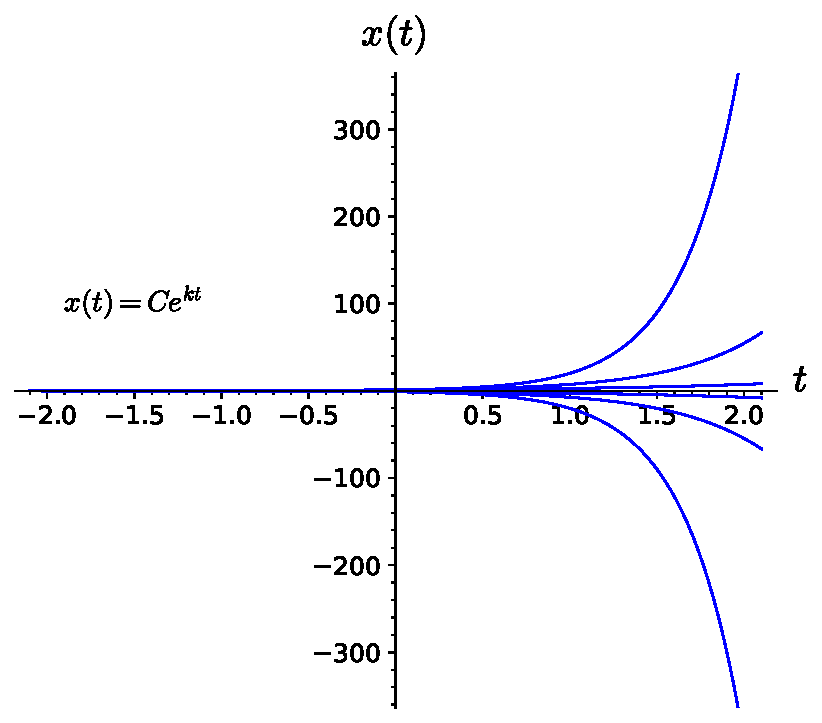
\includegraphics[width=\linewidth]{generated/sageplot/firstlook01-integral-curves.pdf}%
\end{image}%
\tcblower
\end{figureptx}%
\begin{activity}{Verifying Solutions.}{g:activity:idp105545992177680}%
Use direct substitution to verify that \(x(t)\) is a solution of the given differential equation.%
\begin{enumerate}[font=\bfseries,label=(\alph*),ref=\alph*]
\item{}\(y(t) = 4e^{-5t}\); \(y' = -5y\)%
\item{}\(x(t) = 3e^{2t}\); \(x' = 2x\)%
\item{}\(x(t) = 3e^{7t}\); \(x' - 7x = 0\), \(x(0) = 3\)%
\item{}\(x(t) = Ce^{2t} - 5/2\); \(x' = 2x + 5\)%
\item{}\(x(t) = \dfrac{7}{3} e^{3t^2/2} - \dfrac{1}{3}\); \(x' = 3tx + t\), \(x(0) = 2\)%
\end{enumerate}
\end{activity}%
\end{subsectionptx}
%
%
\typeout{************************************************}
\typeout{Subsection 1.1.2 Logistic Growth}
\typeout{************************************************}
%
\begin{subsectionptx}{Logistic Growth}{}{Logistic Growth}{}{}{x:subsection:firstlook01-subsection-logistic-growth}
Not all populations grow exponentially; otherwise, a bacteria culture in a petri dish would grow unbounded and soon be much larger than the size of the laboratory. To see what happens if there are limiting factors to population growth, let us consider the population of fish in a children's trout pond. The number of trout will be limited by the available resources such as food supply as well as by spawning habitat. A small population of fish might grow exponentially if the pond is large and food is abundant, but the growth rate will decline as the population increases and the availability of resources declines.  We can use the \terminology{logistic equation}\index{logistic equation} to model population growth in a resource limited environment.\footnote{The logistic model was first used by the Belgian mathematician and physician Pierre François Verhulst in 1836 to predict the populations of Belgium and France.\label{g:fn:idp105545992153744}}%
\par
To see how the logistic model works, let us try to adjust our model of exponential growth to account for the limited resources of the pond. We will make the following assumptions.%
\begin{itemize}[label=\textbullet]
\item{}If the population of trout is small and the pond is large with abundant resources, the rate of growth will be approximately exponential,%
\begin{equation*}
\frac{dP}{dt} \approx kP.
\end{equation*}
%
\item{}If \(N\) is the maximum population of trout that the pond can support, then any population larger than \(N\) will decrease.  In other words,%
\begin{equation*}
\frac{dP}{dt} \lt 0
\end{equation*}
for \(P \gt N\).  We say that \(N\) is the \terminology{carrying capacity}\index{carrying capacity} for the population.%
\end{itemize}
Our assumptions suggest that we might try an equation of the form%
\begin{equation*}
\frac{dP}{dt} = k f(P) P,
\end{equation*}
where \(f(P)\) is a function of \(P\) that is close to 1 if the population is small but negative if the population is greater than \(N\). The simplest function satisfying these conditions is%
\begin{equation*}
f(P) = \left( 1 - \frac{P}{N} \right).
\end{equation*}
Thus, the \terminology{logistic population model}\index{logistic population model} is given by the differential equation%
\begin{equation*}
\frac{dP}{dt} = k \left( 1 - \frac{P}{N} \right) P.
\end{equation*}
%
\begin{example}{}{x:example:firstlook01-example-logistic-growth}%
Suppose we have a pond that will support 1000 fish, and the initial population is 100 fish. In order to determine the number of fish in the lake at any time \(t\), we must find a solution to the initial value problem%
\begin{align*}
\frac{dP}{dt} & = k \left( 1 - \frac{P}{1000} \right) P\\
P(0) & = 100.
\end{align*}
It is easy to verify that \(P(t) = 1000/(9e^{-kt} + 1)\) is the solution to our initial value problem. Certainly \(P(0) = 100\), and if we differentiate \(P\), we will obtain the righthand side of the differential equation,%
\begin{align*}
\frac{dP}{dt} & = \frac{d}{dt} \left(\frac{1000}{9e^{-kt} + 1}\right)\\
& = 1000 k \frac{9e^{-kt}}{(9e^{-kt} + 1)^2}\\
& = k \frac{9e^{-kt}}{(9e^{-kt} + 1)} \cdot \frac{1000}{9e^{-kt} + 1}\\
& = k \frac{(9e^{-kt} + 1) - 1}{(9e^{-kt} + 1)} \cdot \frac{1000}{9e^{-kt} + 1}\\
& = k \left( 1 - \frac{1000}{1000(9e^{-kt} + 1)}\right) \frac{1000}{9e^{-kt} + 1}\\
& = k \left( 1 - \frac{P}{1000} \right) P.
\end{align*}
In addition, if we know that the population is 200 fish after one year, then%
\begin{equation*}
200 = P(1) = \frac{1000}{9e^{-k} + 1},
\end{equation*}
and we can determine that%
\begin{equation*}
k = \ln\left(  \frac{9}{4}\right) \approx 0.8109.
\end{equation*}
Consequently, the solution to our intial-value problem is%
\begin{equation*}
P(t) = \frac{1000}{9e^{-0.8109 t} + 1}.
\end{equation*}
The graph of our solution certainly fits the situation that we are modeling (\hyperref[x:figure:firstlook01-figure-logistic-growth]{Figure~{\xreffont\ref{x:figure:firstlook01-figure-logistic-growth}}}).  We will learn how to solve initial value problems such as the one described here in \hyperref[x:section:firstlook02]{Section~{\xreffont\ref{x:section:firstlook02}}}. For the time being, we will be satisfied with being able to verify the fact that we have a solution.%
\begin{figureptx}{Logistic growth}{x:figure:firstlook01-figure-logistic-growth}{}%
\begin{image}{0.2}{0.6}{0.2}%
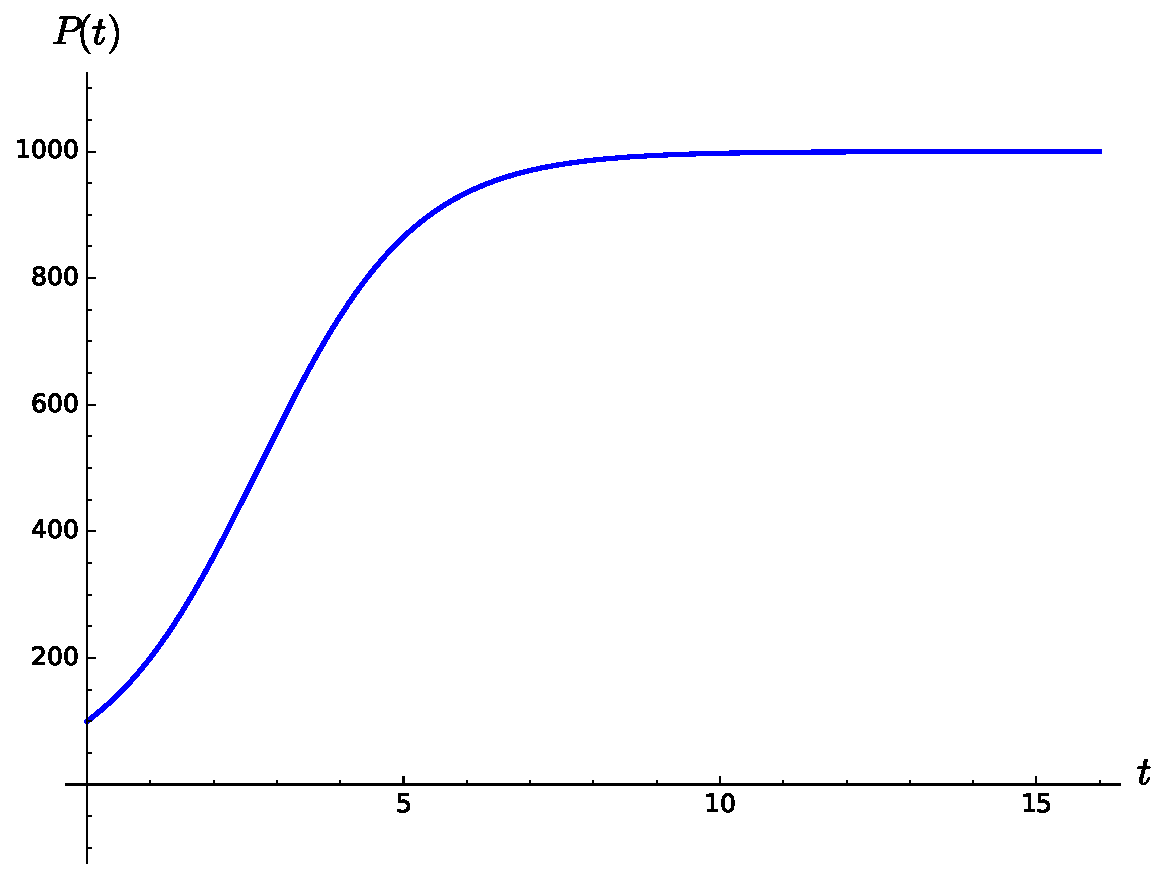
\includegraphics[width=\linewidth]{generated/sageplot/firstlook01-logistic-growth.pdf}%
\end{image}%
\tcblower
\end{figureptx}%
\end{example}
\begin{activity}{Modeling a Population with a Threshhold.}{g:activity:idp105545992201616}%
We can modify the logistic growth model to understand how a population with a minimum threshold grows. The black rhinoceros, once the most numerous of all rhinoceros species, is now critically endangered. The black rhino, native to eastern and southern Africa, was estimated to have a population of about \(100{,}000\) around 1900. Because of hunting, habitat changes, competing species, and most of all illegal poaching, the number of black rhinos today is estimated to be below \(3000\). If the wild population becomes too low, the animals may not be able to find suitable mates and the black rhino will become extinct. There must be a minimum population for the species to survive.  Suppose that this minimum or threshold population for the black rhino is \(1000\) animals and that remaining habitant in Africa will support no more that \(20{,}000\) rhinos. How might we model the current population, \(P(t)\) of black rhinos?%
\begin{enumerate}[font=\bfseries,label=(\alph*),ref=\alph*]
\item{}For what values of \(P\) is the rhino population increasing? What can be said about the value of \(dP/dt\) for these values of \(P\)?%
\par\smallskip%
\noindent\textbf{\blocktitlefont Hint}.\hypertarget{g:hint:idp105545992205968}{}\quad{}(a) The population is increasing if \(dP/dt \gt 0\) and \(1000 \lt P \lt 20000\).%
\item{}For what values of \(P\) is the rhino population decreasing? What can be said about the value of \(dP/dt\) for these values of \(P\)?%
\item{}For what values of \(P\) is the rhino population in equilibrium? What can be said about the value of \(dP/dt\) for these values of \(P\)?%
\item{}Find a differential equation that models the population of rhinos at time \(t\).%
\end{enumerate}
\end{activity}%
\end{subsectionptx}
%
%
\typeout{************************************************}
\typeout{Subsection 1.1.3 A Spring-Mass Model}
\typeout{************************************************}
%
\begin{subsectionptx}{A Spring-Mass Model}{}{A Spring-Mass Model}{}{}{x:subsection:firstlook01-subsection-spring-mass}
Sometimes it is necessary to consider the second derivative when modeling a phenomenon. Suppose that we have a mass lying on a flat, frictionless surface and that this mass is attached to one end of a spring with the other end of the spring attached to a wall. We will denote displacement of the spring by \(x\). If \(x \gt 0\), then the spring is stretched. If \(x \lt 0\), the spring is compressed. If \(x = 0\), then the spring is in a state of equilibrium (\hyperref[x:figure:firstlook01-figure-spring-mass]{Figure~{\xreffont\ref{x:figure:firstlook01-figure-spring-mass}}}). If we pull or push on the mass and release it, then the mass will oscillate back and forth across the table.%
\begin{figureptx}{A spring-mass system}{x:figure:firstlook01-figure-spring-mass}{}%
\begin{image}{0.2}{0.6}{0.2}%
\resizebox{\linewidth}{!}{%
                    \begin{tikzpicture}[scale=0.7]
\draw (-2,0) -- (10,0);
\draw (-2,5) -- (10,5);
\draw (0,0) -- (0,4);
\draw (0,5) -- (0,9);
\filldraw[fill=blue!20,draw=blue!50!black, thick] (4,0) -- (6,0) -- (6,2) -- (4,2) -- cycle;
\draw[ultra thick] (0,1) -- (1,1) (3,1) -- (4,1);
\draw[snake=coil,segment length=5pt,segment amplitude=5pt,ultra thick] (1,1) -- (3,1); 
\filldraw[fill=blue!20,draw=blue!50!black, thick] (7,5) -- (9,5) -- (9,7) -- (7,7) -- cycle;
\draw[ultra thick] (0,6) -- (2,6) (5,6) -- (7,6);
\draw[snake=coil,segment length=7pt,segment amplitude=5pt,ultra thick] (2,6) -- (5,6); 
\draw[dashed] (5,0) -- (5,9);
\node at (5,1) {mass};
\node at (8,6) {mass};
\shadedraw[left color=gray!10,right color=blue!50] (0,0) -- (0,4) -- (-2,4) -- (-2,0) -- cycle;
\shadedraw[left color=gray!10,right color=blue!50] (0,5) -- (0,9) -- (-2,9) -- (-2,5) -- cycle;
\node at (-1,2) {wall};
\node at (-1,7) {wall};
\draw (5,4.9) -- (5,4.3);
\draw (8,4.9) -- (8,4.3);
\draw[<->] (5,4.7) -- (8,4.7);
\node[below] at (5,0) {Position at rest};
\node[below] at (8,4.4) {Position $x(t)$ at time $t$};
\end{tikzpicture}
}%
\end{image}%
\tcblower
\end{figureptx}%
We can construct a differential equation that models our oscillating mass. First, we must consider the restorative force on the spring. We will make the assumption that this force depends on the displacement of the spring, \(F(x)\). Using Taylor's Theorem from calculus, we can expand \(F\) to obtain%
\begin{align*}
F(x) & =  F(0) + F'(0) x + \frac{1}{2} F''(0) x^2 + \cdots\\
& = -k x + \frac{1}{2} F''(0) x^2 + \cdots,
\end{align*}
where \(F'(0) = -k\) and \(F(0) = 0\).  If the displacement is not too large, then \(x^n\) will be small for \(n \geq 2\), and we can ignore higher ordered terms. Thus, we can consider the restorative force on the spring to be proportional to displacement of the spring from its equilibrium length,%
\begin{equation*}
F = -kx.
\end{equation*}
This equation is known as \terminology{Hooke's Law}\index{Hooke's Law}. We can test this law experimentally, and it is reasonably accurate if the displacement of the spring is not too large.%
\par
By Newton's second law of motion, the force on the mass \(m\) must be%
\begin{equation*}
F = ma = m \frac{d^2 x}{dt^2} = m x'',
\end{equation*}
where \(a\) is the acceleration. Setting the two forces equal, we have a \terminology{second-order differential equation}\index{second-order differential equation},%
\begin{equation*}
mx'' = -kx,
\end{equation*}
which describes our oscillating mass. The spring-mass system is an example of a \terminology{harmonic oscillator}\index{harmonic oscillator}. Harmonic oscillators are useful for modeling simple harmonic motion in mechanics.%
\begin{example}{}{x:example:firstlook01-example-harmonic-oscillator}%
Suppose that we have a spring-mass system where \(m =1\) and \(k = 1\). If the initial velocity of the spring is one unit per second and the initial position is at the equilibrium point, then we have the following initial value problem,%
\begin{align*}
x'' + x & =  0\\
x(0) & =  0\\
x'(0) & =  1.
\end{align*}
Since \(x''(t) = - x(t)\) for both the sine and cosine functions, we might guess that a general solution of our differential equation has the form%
\begin{equation*}
x(t) = A \cos t + B \sin t.
\end{equation*}
Noting that%
\begin{equation*}
x'(t) = -A \sin t + B \cos t,
\end{equation*}
and using our initial conditions, we can determine that \(A = 0\) and \(B = 1\) or%
\begin{equation*}
x(t) = \sin t.
\end{equation*}
The graph of the position of the mass as a function of time is given in \hyperref[x:figure:firstlook01-figure-position-mass]{Figure~{\xreffont\ref{x:figure:firstlook01-figure-position-mass}}}.%
\begin{figureptx}{A undamped spring-mass system}{x:figure:firstlook01-figure-position-mass}{}%
\begin{image}{0.15}{0.7}{0.15}%
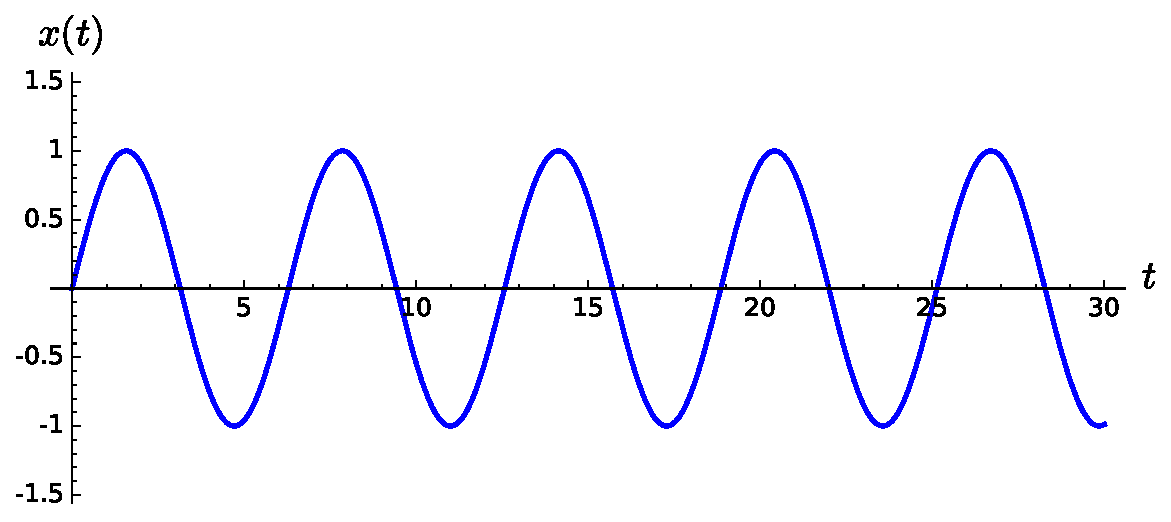
\includegraphics[width=\linewidth]{generated/sageplot/firstlook01-position-mass.pdf}%
\end{image}%
\tcblower
\end{figureptx}%
\end{example}
Now let us add a damping force to our system. For example, we might add a dashpot, a mechanical device that resists motion, to our system. Think of a dashpot as that small cylinder that keeps your screen door from slamming shut. The simplest assumption would be to take the damping force of the dashpot to be proportional to the velocity of the mass, \(x'(t)\). In other words, the harder you try to slam the screen door, the more resistance you will feel. Thus, we have an additional force,%
\begin{equation*}
F = -b x'
\end{equation*}
acting on our mass, where \(b \gt 0\). Our new equation for the spring-mass system is%
\begin{equation*}
mx'' = -bx' - kx.
\end{equation*}
or%
\begin{equation*}
mx'' + bx' + kx = 0,
\end{equation*}
where \(m\), \(b\), and \(k\) are all positive constants. The equation%
\begin{equation*}
mx'' + bx' + kx = 0
\end{equation*}
models a \terminology{simple damped harmonic oscillator}.\index{harmonic oscillator!damped}%
\begin{example}{}{x:example:firstlook01-example-damped-harmonic-oscillator}%
Suppose that we have a spring-mass system governed by the equation%
\begin{equation*}
x'' + 3x' + 2x = 0.
\end{equation*}
Here we let \(m = 1\), \(b = 3\), and \(k = 2\), We will learn how to solve equations of the form \(mx'' + bx' + kx = 0\) in \hyperref[x:chapter:secondorder]{Chapter~{\xreffont\ref{x:chapter:secondorder}}}, but let us assume that the solution is of the form \(x(t) = e^{rt}\) for now. In this case,%
\begin{align*}
x'' + 3x' + 2x & = r^2 e^{rt} + 3 r e^{rt} + 2 e^{rt}\\
& = e^{rt}(r^2 + 3r +2)\\
& = e^{rt}(r+2)(r+1)\\
& = 0.
\end{align*}
Since \(e^{rt}\) is never zero, it must be the case that \(r = -2\) or \(r = -1\), if \(x(t) = e^{rt}\) is to be a solution to our equation. Thus, we might guess that%
\begin{equation*}
x(t) = A e^{-t} + B e^{-2t}
\end{equation*}
is a general solution to our equation. If the initial velocity of our mass is one unit per second and the initial position is zero, then we have the initial value problem%
\begin{align*}
x'' + 3x' + 2 x & = 0\\
x(0) & = 0\\
x'(0) & = 1.
\end{align*}
Using the fact that \(x'(t) = -A e^{-t} -2 B e^{-2t}\), our initial conditions give us the following system of linear equations,%
\begin{align*}
A + B & = 0\\
-A -2B & = 1.
\end{align*}
Thus, \(A = 1\) and \(B = -1\), and our spring-mass system is modeled by the function%
\begin{equation*}
x(t) =  e^{-t} - e^{-2t}.
\end{equation*}
Notice that the additional damping negates any oscillation in the system. In this case, we say that the harmonic oscillator is \terminology{over-damped}\index{harmonic oscillator!over-damped} (\hyperref[x:figure:firstlook01-figure-over-damped]{Figure~{\xreffont\ref{x:figure:firstlook01-figure-over-damped}}}).%
\begin{figureptx}{An over-damped spring-mass system}{x:figure:firstlook01-figure-over-damped}{}%
\begin{image}{0.15}{0.7}{0.15}%
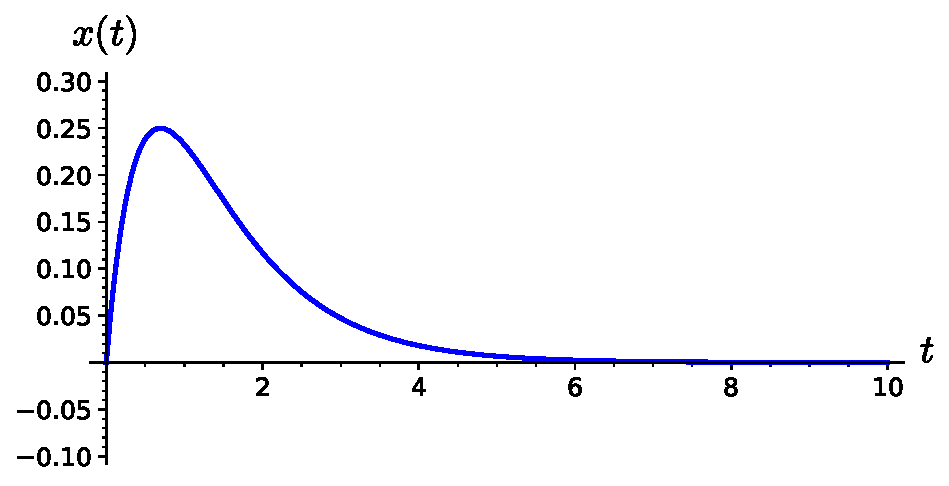
\includegraphics[width=\linewidth]{generated/sageplot/firstlook01-over-damped.pdf}%
\end{image}%
\tcblower
\end{figureptx}%
Of course, if we have a very strong spring and only add a small amount of damping to our spring-mass system, the mass would continue to oscillate, but the oscillations would become progressively smaller. In other words, our harmonic oscillator would be \terminology{under-damped}. \index{harmonic oscillator!under-damped} For example, our spring-mass system might be described by the initial value problem%
\begin{align*}
x'' + 2x' + 50 x & = 0\\
x(0) & = 0\\
x'(0) & = 1.
\end{align*}
It is easy to verify that%
\begin{equation*}
x(t) = \frac{1}{7} e^{-t} \sin 7t
\end{equation*}
is a solution to the initial value problem (\hyperref[x:figure:firstlook01-figure-under-damped]{Figure~{\xreffont\ref{x:figure:firstlook01-figure-under-damped}}}).%
\begin{figureptx}{An under-damped spring-mass system}{x:figure:firstlook01-figure-under-damped}{}%
\begin{image}{0.15}{0.7}{0.15}%
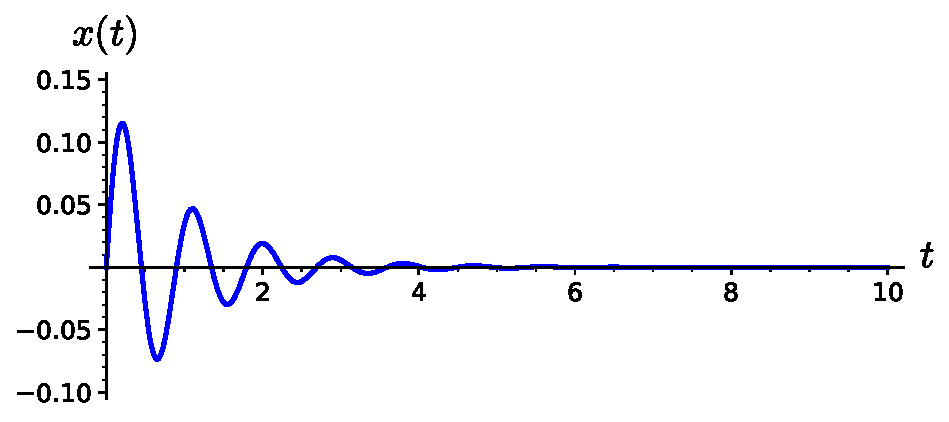
\includegraphics[width=\linewidth]{generated/sageplot/firstlook01-under-damped.pdf}%
\end{image}%
\tcblower
\end{figureptx}%
\end{example}
We will revisit harmonic oscillators and second-order differential equations more fully in \hyperref[x:chapter:secondorder]{Chapter~{\xreffont\ref{x:chapter:secondorder}}}.%
\end{subsectionptx}
%
%
\typeout{************************************************}
\typeout{Subsection 1.1.4 A Predator-Prey System}
\typeout{************************************************}
%
\begin{subsectionptx}{A Predator-Prey System}{}{A Predator-Prey System}{}{}{x:subsection:firstlook01-subsection-predator-prey}
Some situations require more than one differential equation to model a particular phenomenon. We might use a system of differential equations to model two interacting species, say where one species preys on the other.\footnote{The predator-prey model was discovered independently by Lotka (1925) and Volterra (1926).\label{g:fn:idp105545991958544}} For example, we can model how the population of Canadian lynx (\emph{lynx canadenis}) interacts with a the population of snowshoe hare (\emph{lepus americanis}) (see \href{https://www.youtube.com/watch?v=ZWucOrSOdCs}{\nolinkurl{https://www.youtube.com/watch?v=ZWucOrSOdCs}}).%
\par
We have good historical data for the populations of the lynx and snowshoe hare from the Hudson Bay Company, the oldest company in North America. This large Canadian retail company, which owns and operates a large number of retail stores in North America and Europe, including Saks Fifth Avenue, was originally founded in 1670 as a fur trading company. The Hudson Bay Company kept accurate records on the number of lynx pelts that were bought from trappers from 1821 to 1940. The company noticed that the number of pelts varied from year to year and that the number of lynx pelts reached a peak about every ten years \hyperlink{x:biblio:elton-1942}{[{\xreffont 11}]}. The ten year cycle for lynx can be best understood using a system of differential equations.%
\par
The primary prey for the Canadian lynx is the snowshoe hare. We will denote the population of hares by \(H(t)\) and the population of lynx by \(L(t)\), where \(t\) is the time measured in years. We will make the following assumptions for our predator-prey model.%
\begin{itemize}[label=\textbullet]
\item{}If no lynx are present, we will assume that the hares reproduce at a rate proportional to their population and are not affected by overcrowding. That is, the hare population will grow exponentially,%
\begin{equation*}
\frac{dH}{dt} = aH.
\end{equation*}
%
\item{}Since the lynx prey on the hares, we can argue that the rate at which the hares are consumed by the lynx is proportional to the rate at which the hares and lynx interact.  Thus, the equation that predicts the rate of change of the hare population becomes%
\begin{equation*}
\frac{dH}{dt} = aH - bHL.
\end{equation*}
We are thinking of \(HL\) as the number of possible interactions between the lynx and the hare populations.%
\item{}If there is no food, the lynx population will decline at a rate proportional to itself,%
\begin{equation*}
\frac{dL}{dt} = -cL.
\end{equation*}
%
\item{}The lynx receive benefit from the hare population. The rate at which lynx are born is proportional to the number of hares that are eaten, and this is proportional to the rate at which the hares and lynx interact. Consequently, the growth rate of the lynx population can be described by%
\begin{equation*}
\frac{dL}{dt} = -cL + dHL.
\end{equation*}
%
\end{itemize}
We now have a \terminology{system} of differential equations that describe how the two populations interact,%
\begin{align*}
\frac{dH}{dt}  & =  aH - bHL,\\
\frac{dL}{dt}  & =  -cL + dHL.
\end{align*}
We will learn how to analyze and find solutions of systems of differential equations in subsequent chapters; however, we will give a graphical solution in \hyperref[x:figure:firstlook01-figure-lynx-snowshoe-hare]{Figure~{\xreffont\ref{x:figure:firstlook01-figure-lynx-snowshoe-hare}}} to the system%
\begin{align*}
\frac{dH}{dt} & = 0.4H - 0.01HL,\\
\frac{dL}{dt} & = -0.3L + 0.005HL.
\end{align*}
Our graphical solution is obtained using a numerical algorithm (see \hyperref[x:section:firstlook04]{Section~{\xreffont\ref{x:section:firstlook04}}} and \hyperref[x:section:systems03]{Section~{\xreffont\ref{x:section:systems03}}}). Notice that the predator population, \(L\), begins to grow and reaches a peak after the prey population, \(H\) reaches its peak. As the prey population declines, the predator population also declines. Once the predator population is smaller, the prey population has a chance to recover, and the cycle begins again.\footnote{An excellent account of the actual lynx and snowshoe hare data and model can be found in \hyperlink{x:biblio:bauer-2001}{[{\xreffont 5}]}.\label{g:fn:idp105545992002320}}%
\begin{figureptx}{The predator-prey relationship between the lynx and the snowshoe hare}{x:figure:firstlook01-figure-lynx-snowshoe-hare}{}%
\begin{image}{0.2}{0.6}{0.2}%
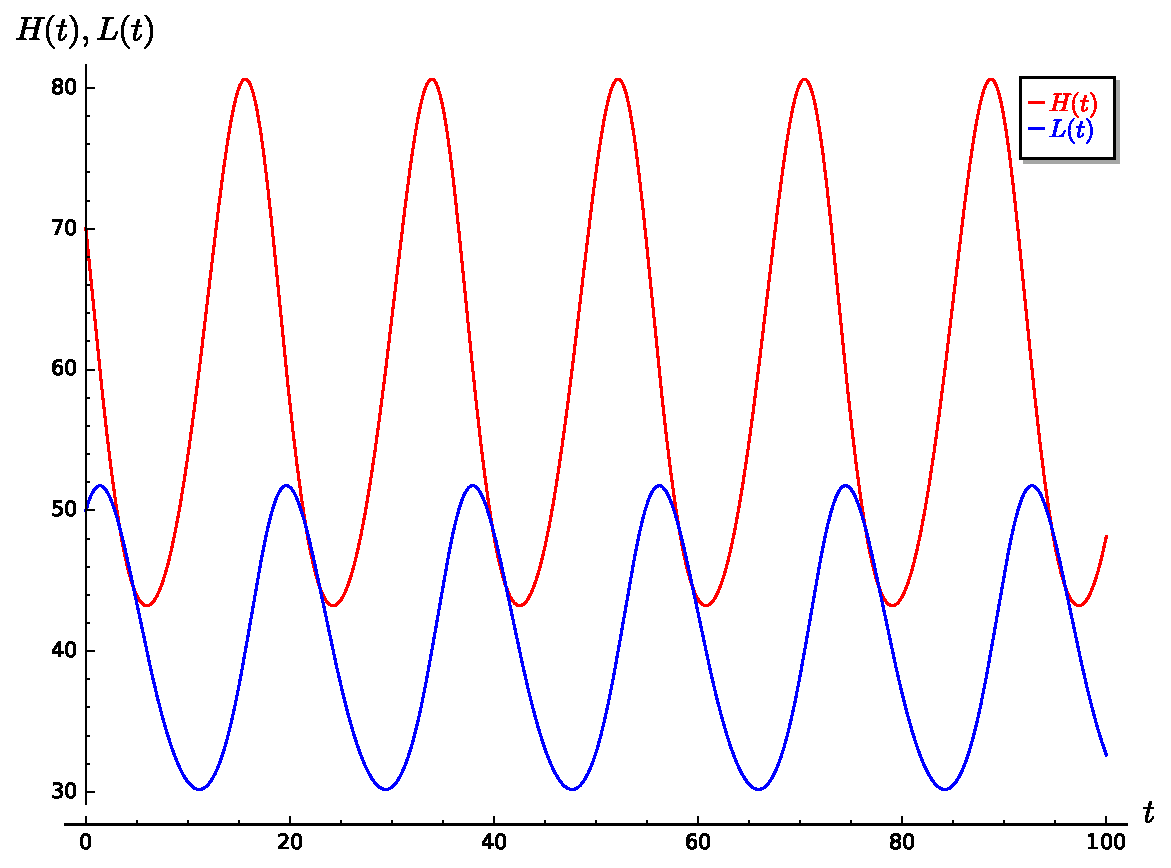
\includegraphics[width=\linewidth]{generated/sageplot/firstlook01-lynx-snowshoe-hare.pdf}%
\end{image}%
\tcblower
\end{figureptx}%
\end{subsectionptx}
%
%
\typeout{************************************************}
\typeout{Subsection 1.1.5 Modeling the HIV-1 Virus}
\typeout{************************************************}
%
\begin{subsectionptx}{Modeling the HIV-1 Virus}{}{Modeling the HIV-1 Virus}{}{}{x:subsection:firstlook01-subsection-modeling-hiv}
The interaction of the HIV-1 virus with the body's immune system can be modeled by a system of differential equations similar to a predator-prey system. After an individual is infected with the HIV-1 virus, the amount of the virus in the bloodstream rises dramatically and the person will often suffer from flu-like symptoms. However, these symptoms will disappear after a period of weeks or months as the body begins to manufacture antibodies against the virus. Tests have been developed to determine the presence of HIV-1 antibodies. If an individual has such antibodies, then they are said to be HIV-1 positive. Once infected with the HIV-1 virus, it can be years before an HIV-positive patient exhibits the full symptoms of AIDS. The body's immune system fights the HIV-1 virus with white blood cells. The CD4-positive T-helper cell, a specific type of white blood cell, is especially important since it helps other cells fight the virus. However, the HIV-1 virus use the CD4-positive T-helper cells to create more virions, destroying the CD4-positive T-helper cells in the process.%
\par
We can develop a system of differential equations to better understand the dynamics of the HIV-1 virus \hyperlink{x:biblio:perelson-2002}{[{\xreffont 20}]}. Let \(V = V(t)\) be the population of the HIV-1 virus at time \(t\). We will assume that the virus concentration is governed by the following differential equation,%
\begin{equation*}
\frac{dV}{dt} = P - cV.
\end{equation*}
The first term, \(P\) is some function of \(t\) that determines the rate at which new viral particles are created. The term \(-cV\) is the death rate for the virions. If someone discovers a drug that blocks the creation of new HIV-1 virions, then \(P\) would be zero and the virions would clear the body at the following rate,%
\begin{equation*}
\frac{dV}{dt} = - cV,
\end{equation*}
and \(V(t) = V_0 e^{-ct}\), where \(V_0\) is the initial viral population.%
\par
Now let us consider a model for the concentration  \(T = T(t)\) of (uninfected) CD4-positive T-helper cells,%
\begin{equation*}
\frac{dT}{dt} = s + pT\left(1 - \frac{T}{T_{\text{max}}}  \right) - d_T T.
\end{equation*}
The constant \(s\) represents the rate at which T-cells are created from sources in the body, such as the thymus. New CD4-positive T-helper cells can also be created from the proliferation of existing CD4-positive T-helper cells, and the second term in the equation represents the logistic growth of the T-cells, where \(p\) is the maximum proliferation rate and \(T_{\text{max}}\) is the T-cell population density where proliferation ceases. Finally, \(d_T\) is the death rate of the T cells.%
\par
Like the influenza virus, the HIV-1 virus is an RNA virus. An RNA virus cannot reproduce on its own and must use the DNA from a host cell. To do this, the virus attaches itself to a CD4-positive T-helper cell and injects its RNA into the cell. This way the virus can use the T-cell's DNA to replicate itself using a process called reverse transcription, where a DNA copy of the virus's RNA is made. New virus particles are created, and the T-cell eventually bursts releasing the virions into the body. If we let \(T^*\) be the concentration of infected T-cells, we can model this process with the following system of equations,%
\begin{align*}
\frac{dT^*}{dt} & =  kTV - \delta T^*\\
\frac{dV}{dt} & =  N \delta T^* - cV,
\end{align*}
where \(\delta\) is the rate of loss of the virus producing T-cells and \(N\) is the number of virions produced per infected T-cell during its lifetime. The term \(kTV\) tells us the rate at which the HIV-1 virus infects T-cells. This is the same idea as modeling how predators interact with prey in a predator-prey model. Thus, our complete model becomes%
\begin{align*}
\frac{dT}{dt} & =  s + pT\left(1 - \frac{T}{T_{\text{max}}}  \right) - d_T T - kTV\\
\frac{dT^*}{dt} & =  kTV - \delta T^*\\
\frac{dV}{dt} & =  N \delta T^* - cV.
\end{align*}
%
\par
One class of drugs that HIV infected patients receive are reverse transcriptase (RT) inhibitors. RT inhibitors block the action of reverse transcription and prevent the virus from duplicating. If one could find the perfect RT inhibitor, then \(k =0\) and our system becomes%
\begin{align*}
\frac{dT}{dt} & = s + pT\left(1 - \frac{T}{T_{\text{max}}}  \right) - d_T T\\
\frac{dT^*}{dt} & = - \delta T^*\\
\frac{dV}{dt} & = N \delta T^* - cV.
\end{align*}
Unfortunately, no one has discovered a perfect RT inhibitor, so we will need to modify the system to account for the effectiveness of the RT inhibitor. We can accomplish this by adding an effectiveness factor, \(1 - \eta\), to the \(kVT\) term. Our system now becomes%
\begin{align*}
\frac{dT}{dt} & =  s + pT\left(1 - \frac{T}{T_{\text{max}}}  \right) - d_T T - k(1 - \eta)TV\\
\frac{dT^*}{dt} & =  k(1 - \eta)TV - \delta T^*\\
\frac{dV}{dt} & =  N \delta T^* - cV.
\end{align*}
If \(\eta = 1\), then the RT inhibitor is completely effective. On the other hand, if \(\eta = 0\), then the RT inhibitor is completely ineffective. We now have a model for how the HIV-1 virus interacts with the immune system. Researchers can use data to estimate the parameters and see exactly what types of solutions are possible.%
\end{subsectionptx}
%
%
\typeout{************************************************}
\typeout{Subsection 1.1.6 Some Questions for Thought}
\typeout{************************************************}
%
\begin{subsectionptx}{Some Questions for Thought}{}{Some Questions for Thought}{}{}{x:subsection:firstlook01-subsection-questions-for-thought}
In this section we have provided a general notion of what a differential equation is as well as several modeling situations where differential equations are useful; however, we have left many questions unanswered.%
\begin{itemize}[label=\textbullet]
\item{}Can we find a more rigorous definition of a differential equation?%
\item{}What is the proper way to define a system of differential equations?%
\item{}Does a differential equation or a system of differential equations always have a solution?%
\item{}Are solutions to differential equations unique?%
\item{}If a unique solution to a differential equation exists, can we find it? If it is not possible to find a precise solution algebraically, can we estimate the solution numerically? If neither is possible, can we still say anything useful about the solution?%
\end{itemize}
Of course, other questions will come to mind as we continue our study of differential equations.%
\end{subsectionptx}
%
%
\typeout{************************************************}
\typeout{Subsection 1.1.7 Important Lessons}
\typeout{************************************************}
%
\begin{subsectionptx}{Important Lessons}{}{Important Lessons}{}{}{x:subsection:firstlook01-subsection-important-lessons}
%
\begin{itemize}[label=\textbullet]
\item{}A \terminology{differential equation} is an equation relating a function to one or more of its derivatives.%
\item{}An \terminology{initial value problem} is a differential equation%
\begin{equation*}
\frac{dx}{dt} = f(t,x),
\end{equation*}
where the \terminology{initial condition}, \(x(t_0) = x_0\), is specified.%
\item{}The three principle steps in modeling any phenomenon with differential equations are:%
\begin{itemize}[label=$\circ$]
\item{}Discovering the differential equation or equations that best describe a specified physical situation.%
\item{}Finding\textemdash{}either exactly or approximately\textemdash{}the appropriate solution of the equation or equations.%
\item{}Interpreting the solution in terms of the phenomenon.%
\end{itemize}
%
\item{}A population that is not affected by overcrowding can be modeled by the differential equation \(P' = kP\) and is said to grow \terminology{exponentially}.%
\item{}A population that must compete for limited resources can be modeled by the \terminology{logistic equation},%
\begin{equation*}
\frac{dP}{dt} = k \left( 1 - \frac{P}{N} \right) P, 
\end{equation*}
where \(N\) is the carrying capacity of the population.%
\item{}Some phenomenon, such as the relationship between a population of predators and a population of prey, are best modeled by systems of differential equations.%
\end{itemize}
%
\end{subsectionptx}
%
%
\typeout{************************************************}
\typeout{Reading Questions 1.1.8 Reading Questions}
\typeout{************************************************}
%
\begin{reading-questions-subsection}{Reading Questions}{}{Reading Questions}{}{}{x:reading-questions:reading-questions-firstlook01}
\begin{introduction}{}%
Textbooks are designed to be read. If you are student enrolled in a course, you should read each section before class. To help your understanding, answer the section's reading questions as preparation for class. If you communicate your answers to your instructor, it will aid your instructor when preparing for your class.%
\end{introduction}%
\begin{divisionexercise}{1}{}{}{x:exercise:reading-questions-firstlook01-1}%
Explain what a differential equation is using your own words.%
\end{divisionexercise}%
\begin{divisionexercise}{2}{}{}{x:exercise:reading-questions-firstlook01-2}%
What does it mean to be a solution to a differential equation?%
\end{divisionexercise}%
\end{reading-questions-subsection}
%
%
\typeout{************************************************}
\typeout{Exercises 1.1.9 Exercises}
\typeout{************************************************}
%
\begin{exercises-subsection}{Exercises}{}{Exercises}{}{}{x:exercises:firstlook01-exercises}
\par\medskip\noindent%
\textbf{Verifying Solutions.}\space\space\hypertarget{x:exercisegroup:firstlook01-exercises-verify-solutions}{}%
Use direct substitution to verify that \(y(t)\) is a solution of the given differential equation in \hyperlink{x:exercisegroup:firstlook01-exercises-verify-solutions}{Exercise Group~{\xreffont 1.1.9.1\textendash{}8}}.%
\begin{exercisegroupcol}{2}
\begin{divisionexerciseegcol}{1}{}{}{x:exercise:firstlook01-exercise-verify-solution-1}%
\(y(t) = e^{4t}\); \(y' = 4y\)%
\end{divisionexerciseegcol}%
\begin{divisionexerciseegcol}{2}{}{}{x:exercise:firstlook01-exercise-verify-solution-2}%
\(y(t) = 3e^{-2t}\); \(y' = -2y\)%
\end{divisionexerciseegcol}%
\begin{divisionexerciseegcol}{3}{}{}{x:exercise:firstlook01-exercise-verify-solution-3}%
\(y(t) = 3e^{5t}\); \(y' - 5y = 0\)%
\end{divisionexerciseegcol}%
\begin{divisionexerciseegcol}{4}{}{}{x:exercise:firstlook01-exercise-verify-solution-4}%
\(y(t) = e^{3t} - 2\); \(y' = 3y + 6\)%
\end{divisionexerciseegcol}%
\begin{divisionexerciseegcol}{5}{}{}{x:exercise:firstlook01-exercise-verify-solution-5}%
\(y(t) = -7e^{t^2} - \dfrac{1}{2}\); \(y' = 2ty + t\)%
\end{divisionexerciseegcol}%
\begin{divisionexerciseegcol}{6}{}{}{x:exercise:firstlook01-exercise-verify-solution-6}%
\(y(t) = (t^8 - t^4)^{1/4}\); \(y' = \dfrac{2y^4 + t^4}{ty^3}\)%
\end{divisionexerciseegcol}%
\begin{divisionexerciseegcol}{7}{}{}{x:exercise:firstlook01-exercise-verify-solution-7}%
\(y(t) = t\); \(y'' - ty' + y = 0\)%
\end{divisionexerciseegcol}%
\begin{divisionexerciseegcol}{8}{}{}{x:exercise:firstlook01-exercise-verify-solution-8}%
\(y(t) = e^t + e^{2t}\); \(y'' - 4y' + 4y = e^t\)%
\end{divisionexerciseegcol}%
\end{exercisegroupcol}
\par\medskip\noindent
\par\medskip\noindent%
\textbf{Finding Solutions.}\space\space\hypertarget{x:exercisegroup:firstlook01-exercises-find-solutions}{}%
Many differential equations have solutions of the form \(y(t) = e^{at}\), where \(a\) is some constant.  For example, \(y(t) = e^{3t}\) is a solution to the equation \(y' = 3y\). Find all values of \(a\) such that \(y(t) = e^{at}\) is a solution to the given equation in \hyperlink{x:exercisegroup:firstlook01-exercises-find-solutions}{Exercise Group~{\xreffont 1.1.9.9\textendash{}14}}.%
\begin{exercisegroupcol}{2}
\begin{divisionexerciseegcol}{9}{}{}{x:exercise:firstlook01-exercise-find-solution-1}%
\(y' = -2y\)%
\end{divisionexerciseegcol}%
\begin{divisionexerciseegcol}{10}{}{}{x:exercise:firstlook01-exercise-find-solution-2}%
\(y' + 7 y = 0\)%
\end{divisionexerciseegcol}%
\begin{divisionexerciseegcol}{11}{}{}{x:exercise:firstlook01-exercise-find-solution-3}%
\(y'' - 3y' + 2y = 0\)%
\end{divisionexerciseegcol}%
\begin{divisionexerciseegcol}{12}{}{}{x:exercise:firstlook01-exercise-find-solution-4}%
\(y'' + 4y' - 12y = 0\)%
\end{divisionexerciseegcol}%
\begin{divisionexerciseegcol}{13}{}{}{x:exercise:firstlook01-exercise-find-solution-5}%
\(y''' - y'' - 4y' + 4y = 0\)%
\end{divisionexerciseegcol}%
\begin{divisionexerciseegcol}{14}{}{}{x:exercise:firstlook01-exercise-find-solution-6}%
\(y^{(5)} - 5y''' + 4y' = 0\)%
\end{divisionexerciseegcol}%
\end{exercisegroupcol}
\par\medskip\noindent
\par\medskip\noindent%
\textbf{Initial Value Problems.}\space\space\hypertarget{x:exercisegroup:firstlook01-exercises-ivps}{}%
Use direct substitution to verify that \(y(t)\) is a solution of the given differential equation in \hyperlink{x:exercisegroup:firstlook01-exercises-ivps}{Exercise Group~{\xreffont 1.1.9.15\textendash{}20}}. Then use the initial conditions to determine the constants \(C\) or \(c_1\) and \(c_2\).%
\begin{exercisegroup}
\begin{divisionexerciseeg}{15}{}{}{x:exercise:firstlook01-exercise-ivp-1}%
\(y' = 4y\), \(y(0) = 2\), \(y(t) = Ce^{4t}\)%
\end{divisionexerciseeg}%
\begin{divisionexerciseeg}{16}{}{}{x:exercise:firstlook01-exercise-ivp-2}%
\(y' + 7 y = 0\), \(y(0) = 2\), \(y(t) = C e^{-7t}\)%
\end{divisionexerciseeg}%
\begin{divisionexerciseeg}{17}{}{}{x:exercise:firstlook01-exercise-ivp-3}%
\(y'' + 4y = 0\), \(y(0) = 1\), \(y'(0) = 0\), \(y(t) = c_1 \cos 2t + c_2 \sin 2t\)%
\end{divisionexerciseeg}%
\begin{divisionexerciseeg}{18}{}{}{x:exercise:firstlook01-exercise-ivp-4}%
\(y'' - 5y' + 4y = 0\), \(y(0) = 1\), \(y'(0) = 0\), \(y(t) = c_1 e^t + c_2 e^{4t}\)%
\end{divisionexerciseeg}%
\begin{divisionexerciseeg}{19}{}{}{x:exercise:firstlook01-exercise-ivp-5}%
\(y'' + 4y' + 13y = 0\), \(y(0) = 1\), \(y'(0) = 0\), \(y(t) = c_1 e^{-2t} \cos 3t + c_2 e^{-2t} \sin 3t\)%
\end{divisionexerciseeg}%
\begin{divisionexerciseeg}{20}{}{}{x:exercise:firstlook01-exercise-ivp-6}%
\(y'' - 4y' + 4y = 0\), \(y(0) = 1\), \(y'(0) = 0\), \(y(t) = c_1 e^{2t} + c_2 te^{2t}\)%
\end{divisionexerciseeg}%
\end{exercisegroup}
\par\medskip\noindent
\par\medskip\noindent%
\textbf{Boundary Value Problems.}\space\space\hypertarget{x:exercisegroup:firstlook01-exercises-bv}{}%
Use direct substitution to verify that \(y(t)\) is a solution of the given differential equation in \hyperlink{x:exercisegroup:firstlook01-exercises-bv}{Exercise Group~{\xreffont 1.1.9.21\textendash{}24}}.  Then use the boundary conditions to determine the constants \(c_1\) and \(c_2\) (if possible).%
\begin{exercisegroup}
\begin{divisionexerciseeg}{21}{}{}{x:exercise:firstlook01-exercise-bv-1}%
\(y'' + 4y = 0\), \(y(0) = 1\), \(y(\pi) = 0\), \(y(t) = c_1 \cos 2t + c_2 \sin 2t\)%
\end{divisionexerciseeg}%
\begin{divisionexerciseeg}{22}{}{}{x:exercise:firstlook01-exercise-bv-2}%
\(y'' - 5y' + 4y = 0\), \(y(0) = 1\), \(y(1) = 0\), \(y(t) = c_1 e^t + c_2 e^{4t}\)%
\end{divisionexerciseeg}%
\begin{divisionexerciseeg}{23}{}{}{x:exercise:firstlook01-exercise-bv-3}%
\(y'' + 4y' + 13y = 0\), \(y(0) = 1\), \(y(\pi) = 0\), \(y(t) = c_1 e^{-2t} \cos 3t + c_2 e^{-2t} \sin 3t\)%
\end{divisionexerciseeg}%
\begin{divisionexerciseeg}{24}{}{}{x:exercise:firstlook01-exercise-bv-4}%
\(y'' - 4y' + 4y = 0\), \(y(0) = 1\), \(y(1) = 0\), \(y(t) = c_1 e^{2t} + c_2 te^{2t}\)%
\end{divisionexerciseeg}%
\end{exercisegroup}
\par\medskip\noindent
\begin{divisionexercise}{25}{}{}{x:exercise:firstlook01-exercise-yprime-yx2-y}%
Consider the differential equation \(y' = y(2 - y)\).%
\begin{enumerate}[label=(\alph*)]
\item{}Verify that \(y(t) = 2/(1 + Ce^{-2t})\) is a solution to this equation.%
\item{}Sketch solution curves for  \(C = 1, 2, \ldots, 5\).%
\item{}Verify that \(y = 0\) is a solution to the differential equation in part (a).  Can you find a value for \(C\) such that%
\begin{equation*}
y(t) = \frac{2}{1 + Ce^{-2t}} = 0?
\end{equation*}
%
\end{enumerate}
%
\end{divisionexercise}%
\begin{divisionexercise}{26}{}{}{x:exercise:firstlook01-exercise-y-double-prime-plus-9y}%
Consider the differential equation \(y'' + 9y = 0\).%
\begin{enumerate}[label=(\alph*)]
\item{}Verify that \(y(t) = c_1 \cos 3t + c_2 \sin 3t\) is a solution to this equation.%
\item{}Sketch solution curves for  \(c_1 = 1\) and \(c_2 = 1, 2, \ldots, 5\).%
\end{enumerate}
%
\end{divisionexercise}%
\begin{divisionexercise}{27}{}{}{x:exercise:firstlook01-exercise-rabbit-population}%
The growth of a population of rabbits with unlimited resources and space can be modeled by the exponential growth equation, \(dP/dt = kP\).%
\begin{enumerate}[label=(\alph*)]
\item{}Write a differential equation to model a population of rabbits with unlimited resources, where hunting is allowed at a constant rate \(\alpha\).%
\item{}Write a differential equation to model a population of rabbits with unlimited resources, where hunting is allowed at a rate proportional to the population of rabbits.%
\item{}Write a differential equation to model a population of rabbits with limited resources, where hunting is allowed at a constant rate \(\alpha\).%
\item{}Write a differential equation to model a population of rabbits with limited resources, where hunting is allowed at a rate proportional to the population of rabbits.%
\end{enumerate}
%
\end{divisionexercise}%
\begin{divisionexercise}{28}{}{}{x:exercise:firstlook01-exercise-first-order-linear}%
Given the equation \(x' + a x = q(t)\), where \(a\) is a constant and \(q(t)\) is a continuous function defined on an interval \(I\), show that%
\begin{equation*}
x(t) = Ce^{-at} + e^{-at} \int_{t_0}^t e^{as}q(s) \, ds
\end{equation*}
is a solution of this equation, where \(c\) is any constant and \(t_0 \in I\).%
\par\smallskip%
\noindent\textbf{\blocktitlefont Hint}.\hypertarget{g:hint:idp105545992060560}{}\quad{}Rewriting the differential equation as \(x' + a x - q(t) = 0\) and using the fact that%
\begin{equation*}
x'(t) = -a Ce^{-at} - a e^{-at} \int_{t_0}^t e^{as}q(s) \, ds + b(t),
\end{equation*}
we see that%
\begin{align*}
x'(t) + a x(t) - q(t) & = -a Ce^{-at} - a e^{-at} \int_{t_0}^t e^{as}q(s) \, ds + q(t)\\
& + \; aCe^{-at} + ae^{-at} \int_{t_0}^t e^{as}q(s) \, ds - q(t)\\
& = 0.
\end{align*}
%
\end{divisionexercise}%
\begin{divisionexercise}{29}{Radiocarbon Dating.}{}{x:exercise:firstlook01-exercise-radio-carbon-dating}%
Carbon 14 is a radioactive isotope of carbon, the most common isotope of carbon being carbon 12. Carbon 14 is created when cosmic ray bombardment changes nitrogen 14 to carbon 14 in the upper atmosphere. The resulting carbon 14 combines with atmospheric oxygen to form radioactive carbon dioxide, which is incorporated into plants by photosynthesis. Animals acquire carbon 14 by eating plants. When an animal or plant dies, it ceases to take on carbon 14, and the amount of isotope in the organism begins to decay into the more common carbon 12. Carbon 14 has a very long half-life, about 5730 years. That is, given a sample of carbon 14, it will take 5730 years for half of the sample to decay to carbon 12. The long half-life is what makes carbon 14 dating very useful in dating objects from antiquity.\index{radio carbon dating}%
\begin{enumerate}[label=(\alph*)]
\item{}Consider a sample of material that contains \(A(t)\) atoms of carbon 14 at time \(t\). During each unit of time a constant fraction of the radioactive atoms will spontaneously decay into another element or a different isotope of the same element. Thus, the sample behaves like a population with a constant death rate and a zero birth rate.  Make use of the model of exponential growth to construct a differential equation that models radioactive decay for carbon 14.%
\item{}Solve the equation that you proposed in (a) to find an explicit formula for \(A(t)\).%
\item{}The Chauvet-Pont-d'Arc Cave in the Ardèche department of southern France contains some of the best preserved cave paintings in the world. Carbon samples from torch marks and from the paintings themselves, as well as from animal bones and charcoal found on the cave floor, have been used to estimate the age of the cave paintings. If a particular sample taken from the Cauvet Cave contains 2\% of the expected carbon 14, what is the approximate age of the sample?%
\end{enumerate}
%
\end{divisionexercise}%
\begin{divisionexercise}{30}{}{}{x:exercise:firstlook01-exercise-predator-prey}%
Consider the following predator-prey systems of differential equations%
\begin{align*}
\frac{dx}{dt} \amp =  -\frac{x}{2} + \frac{xy}{2 + y},\\
\frac{dy}{dt} \amp=  y(1 - y) - \frac{xy}{2 + y}.
\end{align*}
%
\begin{enumerate}[label=(\alph*)]
\item{}Which equation models the prey population and which equation models the predator population?%
\item{}How does the prey population grow if there are no predators present?%
\item{}What happens if there are a lot of prey present?%
\end{enumerate}
%
\par\smallskip%
\noindent\textbf{\blocktitlefont Hint}.\hypertarget{g:hint:idp105545991839248}{}\quad{}Think about the limit of the interaction term as the number of prey becomes very large.%
\end{divisionexercise}%
\end{exercises-subsection}
%
%
\typeout{************************************************}
\typeout{Subsection 1.1.10 An Introduction to \emph{Sage}}
\typeout{************************************************}
%
\begin{subsectionptx}{An Introduction to \emph{Sage}}{}{An Introduction to \emph{Sage}}{}{}{x:subsection:firstlook01-subsection-sage}
Technology can prove very useful when studying differential equations. Software packages such Maple, Mathematica, and Matlab each have their advantages and disadvantages. We will use \emph{Sage}, a readily available open source computer algebra system, as our choice of software. \emph{Sage} can be run on an individual computer or over the Internet on a server. You can even access \emph{Sage} from your smart phone. For our purposes, \emph{Sage} cells are embedded into the textbook, so there is nothing to install on your computer. Simply, evaluate the cell. You can even change the preloaded commands in the cell if you wish. For example, let us evaluate the derivative of \(f(x) = x^2 \cos x\).%
\begin{sageinput}
x = var('x') #declare x as a variable
y = x^2*cos(x)  #set y equal to x^2*cos(x)
solution = diff(y, x) #differentiate y with respect to x
solution.show() #display the solutions in a nice format
\end{sageinput}
\begin{sageoutput}
-x^2*sin(x) + 2*x*cos(x)
\end{sageoutput}
Note that anything following a pound sign \mono{\#} is a comment.%
\par
We can use \emph{Sage} to plot functions. For example, we can plot the function \(f(x) = x^2 \cos x\) as well as its derivative on the same graph.%
\begin{sageinput}
x = var('x')
y = x^2*cos(x)
yprime = diff(y, x)
p = plot(y, (x, -2, 2), color ='blue', legend_label='$f$', legend_color='blue')
p += plot(yprime, (x, -2, 2), color='red', legend_label='$df/dx$', legend_color='red')
p
\end{sageinput}
We can use \emph{Sage} to solve differential equations. Suppose that we wish to solve the initial value problem%
\begin{align*}
\frac{dP}{dt} & = kP\\
P(0) & = 1000.
\end{align*}
We can use the following commands.%
\begin{sageinput}
k,t = var('k, t') #declare variables k and t
P = function('P')(t) #declare P to be a function of t
de = diff(P, t) == k*P  #differential equation
#solve specifying initial conditions
#and independent variable solution
solution = desolve(de, P, ivar=t, ics=[0, 1000]) 
solution.show()
\end{sageinput}
\begin{sageoutput}
1000*e^(k*t)
\end{sageoutput}
We will provide abundant examples of how to use \emph{Sage} to solve and analyze differential equations throughout the book, and we encourage the reader to experiment by altering the \emph{Sage} commands inside the individual \emph{Sage} cells. If you make a mistake, you can simply reload the webpage and start again.%
\par
The reader will find plenty of resources to learn how to use \emph{Sage}. A good place to start is \href{http://www.sagemath.org/help.html}{\nolinkurl{www.sagemath.org/help.html}}, \hyperlink{x:biblio:bard-2015}{[{\xreffont 1}]}, or the UTMOST Sage Cell Repository (\href{http://utmost-sage-cell.org}{\nolinkurl{utmost-sage-cell.org}}), which contains several hundred Sage cells that can be excuted right from the repository website. Although we will be using \emph{Sage} as the technology of choice, much of this book can be read independently of \emph{Sage}. Finally, we would like to emphasize once again that the reader who chooses not to use some sort of technology will be at a disadvantage.%
%
%
\typeout{************************************************}
\typeout{Exercises 1.1.10 \emph{Sage} Exercises}
\typeout{************************************************}
%
\begin{exercises-subsubsection-numberless}{\emph{Sage} Exercises}{}{\emph{Sage} Exercises}{}{}{x:exercises:firstlook01-sage-exercises}
\begin{divisionexercise}{1}{}{}{x:exercise:firstlook01-sage-exercise-evaluate}%
In the \emph{Sage} cell below enter \mono{2 + 2} and then evaluate the cell. Your answer should be \mono{4} of course.  Next try entering \mono{2\textasciicircum{}1000}. You should see a very large number.%
\begin{sageinput}

\end{sageinput}
\begin{sageoutput}

\end{sageoutput}
\end{divisionexercise}%
\end{exercises-subsubsection-numberless}
\end{subsectionptx}
\end{sectionptx}
%
%
\typeout{************************************************}
\typeout{Section 1.2 Separable Differential Equations}
\typeout{************************************************}
%
\begin{sectionptx}{Separable Differential Equations}{}{Separable Differential Equations}{}{}{x:section:firstlook02}
\begin{objectives}{Objectives}{g:objectives:idp105545991825168}
%
\begin{itemize}[label=\textbullet]
\item{}To understand that a differential equation of \terminology{order} \(n\) is an equation that can be put in the form%
\begin{equation*}
F(t, x, x', x'', \ldots, x^{(n)}) = 0,
\end{equation*}
where \(F\) is a function of \(n + 2\) variables, and to understand that a \terminology{solution} to the equation on an interval \(I = (a, b)\) is a function \(u = u(t)\) such that the first \(n\) derivatives of \(u\) are defined on \(I\), and%
\begin{equation*}
F(t, u, u', u'', \ldots, u^{(n)}) = 0.
\end{equation*}
%
\item{}To understand that a \terminology{first-order differential equation} is an equation that can be written in the form%
\begin{equation*}
\frac{dx}{dt} = f(t, x).
\end{equation*}
%
\item{}To understand that a differential equation is \terminology{separable} if it can be written in the form%
\begin{equation*}
\frac{dy}{dx} =M(x) N(y),
\end{equation*}
and by rewriting the equation in the form%
\begin{equation*}
g(y) \, dy = f(x) \, dx
\end{equation*}
the equation can be solved by integrating both sides.%
\end{itemize}
\end{objectives}
\begin{introduction}{}%
We will define a \terminology{differential equation}\index{differential equation} of \terminology{order}\index{differential equation!order} \(n\) to be an equation that can be put in the form%
\begin{equation*}
F(t, x, x', x'', \ldots, x^{(n)}) = 0,
\end{equation*}
where \(F\) is a function of \(n + 2\) variables. A \terminology{solution}\index{differential equation!solution} to this equation on an interval \(I = (a, b)\) is a function \(u = u(t)\) such that the first \(n\) derivatives of \(u\) are defined on \(I\), and%
\begin{equation*}
F(t, u, u', u'', \ldots, u^{(n)}) = 0.
\end{equation*}
We will concentrate on first-order differential equations in this chapter. That is, we will consider equations of the form%
\begin{equation*}
\frac{dx}{dt} = f(t, x).
\end{equation*}
%
\end{introduction}%
%
%
\typeout{************************************************}
\typeout{Subsection 1.2.1 Separable Differential Equations}
\typeout{************************************************}
%
\begin{subsectionptx}{Separable Differential Equations}{}{Separable Differential Equations}{}{}{x:subsection:firstlook02-subsection-separable-de}
In general, we cannot generally find such a formula for an arbitrary first-order differential equation. We can, however, solve a differential equation \(y' = f(x, y)\) if we can write the equation in the form%
\begin{equation*}
f(x) + g(y) \frac{dy}{dx} = 0.
\end{equation*}
Such equations are called \terminology{separable}\index{differential equation!separable}. We can solve separable equations by integrating the first term with respect to \(x\) and the second term with respect to \(y\).%
\begin{example}{}{g:example:idp105545991876496}%
Suppose that we wish to solve the initial value problem%
\begin{align*}
\frac{dy}{dx} & =  xy\\
y(0) & = 1.
\end{align*}
We can rewrite this equation in the form%
\begin{equation*}
\frac{1}{y} \frac{dy}{dx} = x
\end{equation*}
or in the alternate form%
\begin{equation*}
\frac{1}{y} \, dy = x \, dx.
\end{equation*}
Integrating both sides of the equation, we have%
\begin{equation*}
\ln |y| = \frac{1}{2} x^2 + C,
\end{equation*}
where \(C\) is an arbitrary constant. Using the initial condition, \(y(0) = 1\) to find \(C\), we see that%
\begin{equation*}
0 = \ln|1| = 0 + C.
\end{equation*}
Thus, the solution to our initial value problem can be given implicitly by \(\ln y = x^2/2\). In this example, we can actually write down an explicit solution that is defined everywhere,%
\begin{equation*}
y = e^{x^2/2}.
\end{equation*}
The \emph{Sage} commands for solving our initial value problem are below.%
\begin{sageinput}
x = var('x') #declare x as a variable
y = function('y')(x) #declare y as a function of x
de = diff(y, x) == x*y #write the differential equation
solution = desolve(de, y, ics=[0, 1]) #find the solution
solution
\end{sageinput}
\begin{sageoutput}
e^(1/2*x^2)
\end{sageoutput}
\end{example}
If we ask \emph{Sage} to solve a differential equation that it cannot solve analytically, the computation will return an error. \emph{Sage} will not solve the initial value problem%
\begin{align*}
\frac{dy}{dx} & =  \sin(xy)\\
y(0) & =  1.
\end{align*}
%
\begin{sageinput}
x = var('x')
y = function('y')(x)
de = diff(y, x) == sin(x*y)
solution = desolve(de, y, ics=[0, 1])
solution
\end{sageinput}
\begin{example}{}{g:example:idp105545991884176}%
Consider the initial value problem%
\begin{align*}
\frac{dy}{dt} & =  \frac{t}{y - t^2y}\\
y(0) & = 4.
\end{align*}
First, we separate the variables of the equations and write%
\begin{equation*}
y \, dy = \frac{t}{1 - t^2} \, dt.
\end{equation*}
Integrating both sides of the equation, we have%
\begin{equation*}
\frac{1}{2} y^2 = - \frac{1}{2} \ln|1 - t^2| + C \qquad \text{or} \qquad y^2 = - \ln|1 - t^2| + C.
\end{equation*}
Using the initial condition, \(y(0) = 4\), we can determine the value of \(C\),%
\begin{equation*}
y^2 = 16 - \ln|1 - t^2| \qquad \text{or} \qquad y = \sqrt{16 - \ln|1 - t^2| }.
\end{equation*}
Notice that the solution does not make sense for all values of \(t\). In fact, the solution is only defined on the interval \(-1 \lt t \lt 1\), if we require that our solution be continuous. Let us see what \emph{Sage} has to say.%
\begin{sageinput}
t = var('t')
y = function('y')(t)
de = diff(y, t) == t/(y - t^2*y)
solution = desolve(de, y, ics=[0, 4])
solution
\end{sageinput}
\begin{sageoutput}
-1/2*y(t)^2 == -1/2*I*pi + 1/2*log(t + 1) + 1/2*log(t - 1) - 8
\end{sageoutput}
\emph{Sage} does return a solution even if it looks a bit different than the one that we arrived at above. Notice that we have an imaginary term in our solution, where \(i^2 = -1\). We will examine the role of complex numbers and how useful they are in the study of ordinary differential equations in a later chapter, but for the moment complex numbers will just muddy the situation.%
\end{example}
\begin{example}{}{g:example:idp105545991857168}%
The initial value problem in \hyperref[x:example:firstlook01-example-logistic-growth]{Example~{\xreffont\ref{x:example:firstlook01-example-logistic-growth}}} is a good example of a separable differential equation,%
\begin{align*}
\frac{dP}{dt} & = k \left( 1 - \frac{P}{1000} \right) P\\
P(0) & = 100.
\end{align*}
Using partial fractions, we can rewrite this equation as%
\begin{equation}
\frac{1000}{P(1000 - P)} \, dP = \left( \frac{1}{P} + \frac{1}{1000-P}\right) \, dP = k \, dt.\label{x:men:firstlook02-equation-logistic-IVP}
\end{equation}
Integrating both sides of \hyperref[x:men:firstlook02-equation-logistic-IVP]{({\xreffont\ref{x:men:firstlook02-equation-logistic-IVP}})}, we obtain%
\begin{equation*}
\ln|P| - \ln|1000 - P| = \ln \left|\frac{P}{1000 - P}\right| = kt + C.
\end{equation*}
Taking the exponential of both sides yields%
\begin{equation*}
\frac{P}{1000 - P} = e^{kt + C} = e^{kt} e^C.
\end{equation*}
Since \(C\) is an arbitrary constant, we know that \(e^C\) is an arbitrary positive constant, which we will also call \(C\). So we can rewrite this last equation as%
\begin{equation*}
P = Ce^{kt} (1000 - P) = 1000 Ce^{kt} - Ce^{kt}P.
\end{equation*}
Solving for \(P\) yields%
\begin{equation*}
P = \frac{1000Ce^{kt}}{Ce^{kt} + 1} = \frac{1000}{Ce^{-kt} + 1}.
\end{equation*}
Using our initial condition \(P(0) = 100\), we can determine that \(C = 9\).%
\end{example}
\begin{activity}{Solving Separable Differential Equations.}{g:activity:idp105545991863440}%
Solve each of the following differential equations using the separation of variables technique.%
\begin{enumerate}[font=\bfseries,label=(\alph*),ref=\alph*]
\item{}\(dy/dx = y/x\)%
\item{}\((x^2 + 1)y' = xy\)%
\item{}\(dx/dt = e^x \sqrt{t}\)%
\item{}\(\dfrac{dx}{dt} = \dfrac{\sec^2 t + 2t}{2x}\), \(x(0) = -2\)%
\item{}\(dy/dx = \sqrt{xy}\), \(y(1) = 3\)%
\end{enumerate}
\end{activity}%
\end{subsectionptx}
%
%
\typeout{************************************************}
\typeout{Subsection 1.2.2 Newton's Law of Cooling}
\typeout{************************************************}
%
\begin{subsectionptx}{Newton's Law of Cooling}{}{Newton's Law of Cooling}{}{}{x:subsection:firstlook02-subsection-newtons-law-cooling}
Separable equations arise in a wide range of application problems. One does not have to watch too many crime dramas to realize that the time of death of a murder victim is an important question in many criminal investigations. How does a forensic scientist or a medical examiner determine the time of death? Human beings have a temperature of \(98.6^\circ\)F. If the surrounding temperature is cooler, then the body will cool down after death. Eventually, the temperature of the body will match the temperature of the environment. We should not expect the body to cool at a constant rate either. Think of how a hot cup of coffee or tea cools. The liquid will cool quite quickly during the first few minutes but will remain relatively warm for quite a long period.%
\par
The answer to our forensic question can be found by using \terminology{Newton's law of cooling}\index{Newton's law of cooling}, which tells us that the rate of change of the temperature of an object is proportional to the difference between the temperature of the object and the temperature of the surrounding medium. Newton's law of cooling can be easily stated as a differential equation,%
\begin{equation*}
\frac{dT}{dt} = k(T - T_m),
\end{equation*}
where \(T\) is the temperature of the object, \(T_m\) is the temperature of the surrounding medium, and \(k\) is the proportionality constant.%
\par
Suppose that the temperature of the surrounding environment is \(70^\circ\)F, and we know from experience that a body under these conditions cools off approximately \(2^\circ\)F during the first hour after death.  In order to determine a formula for the time of death, we must solve the initial value problem%
\begin{align*}
\frac{dT}{dt} & =  k(T - 70)\\
T(0) & =  98.6,
\end{align*}
where \(T(1) = 96.6\). If we rewrite the equation%
\begin{equation*}
\frac{dT}{dt} = k(T - 70) 
\end{equation*}
as%
\begin{equation*}
\frac{1}{T - 70} \frac{dT}{dt} = k,
\end{equation*}
we see that this equation is separable.  Integrating both sides of the last equation, we obtain \(\ln | T - 70| = kt + C\). Since we are assuming that \(T \gt 70\), we can write \(T - 70\) instead of \(|T - 70|\).  Thus, we have%
\begin{equation*}
\ln( T- 70) = kt + C \qquad \text{or} \qquad T - 70 = e^{kt + C} = e^{kt}e^C.
\end{equation*}
Letting \(D = e^C\), the solution becomes%
\begin{equation*}
T(t) = D e^{kt} + 70.
\end{equation*}
The initial condition, \(T(0) = 98.6\), tells us that \(D = 28.6\). Thus,%
\begin{equation*}
T(t) = 28.6 e^{kt} + 70.
\end{equation*}
Since%
\begin{equation*}
96.6 = T(1) =28.6 e^{k \cdot 1} + 70,
\end{equation*}
we can determine the constant \(k\) to be%
\begin{equation*}
k = \ln\left( \frac{26.6}{28.6} \right) \approx -0.0725.
\end{equation*}
and%
\begin{equation*}
T(t) =28.6 e^{-0.0725 t} + 70.
\end{equation*}
The graph of the \(T\) seems appropriate to our model (\hyperref[x:figure:firstlook02-figure--newton-cooling]{Figure~{\xreffont\ref{x:figure:firstlook02-figure--newton-cooling}}}).%
\begin{figureptx}{Newton's law of cooling}{x:figure:firstlook02-figure--newton-cooling}{}%
\begin{image}{0.2}{0.6}{0.2}%
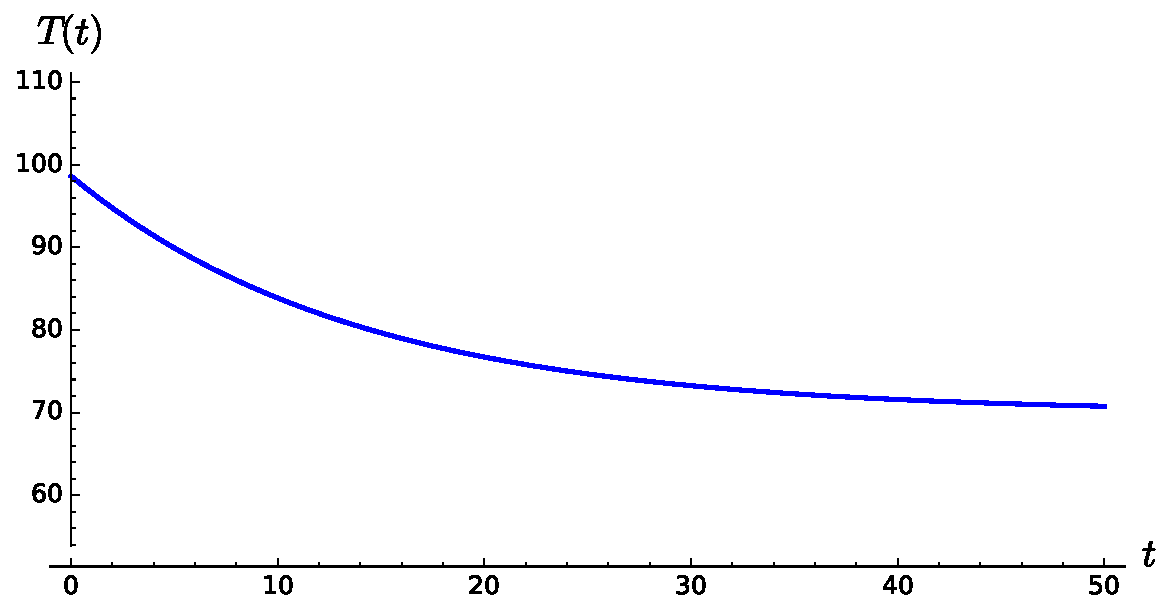
\includegraphics[width=\linewidth]{generated/sageplot/firstlook02-newton-cooling.pdf}%
\end{image}%
\tcblower
\end{figureptx}%
Let us solve our differential equation using \emph{Sage}.%
\begin{sageinput}
k,t = var('k,t')
T = function('T')(t)
de = diff(T,t) == k*(T - 70)
solution = desolve(de, T, ivar=t)
solution.show()
\end{sageinput}
\begin{sageoutput}
(c + 70*e^(-k*t))*e^(k*t)
\end{sageoutput}
We can use \emph{Sage} to plot our solution.%
\begin{sageinput}
t = var('t')
T(t) = 28.6 * exp(-0.0725 * t) + 70
plot(T, (t, 0, 24))
\end{sageinput}
\begin{sageoutput}

\end{sageoutput}
\begin{activity}{Coffee Temperature.}{g:activity:idp105545991885328}%
The brewing temperature of the water used is very important. It should be between \(195^\circ\)F and \(205^\circ\)F. The closer to \(205^\circ\)F the better. Boiling water (\(212^\circ\)F) should never be used, as it will burn the coffee. Water that is less than \(195^\circ\)F will not extract properly. On the other hand, coffee that has a temperature of \(205^\circ\)F is too hot to drink.\footnotemark{}  Coffee is best when it is served at a temperature of \(140^\circ\)F to \(155^\circ\)F (the Goldilocks range).%
\begin{enumerate}[font=\bfseries,label=(\alph*),ref=\alph*]
\item\label{x:task:firstlook02-task-coffee}Suppose coffee is initially brewed at \(205^\circ\)F.  If room temperature is \(70^\circ\)F, set up an initial value problem to model the temperature of the coffee at time \(t\), where \(t\) is the time in minutes after brewing has finished.%
\item{}Solve the initial value problem from \hyperref[x:task:firstlook02-task-coffee]{Task~{\xreffont\ref{g:activity:idp105545991885328}}.{\xreffont\ref{x:task:firstlook02-task-coffee}}}%
\item{}If the temperature of the coffee drops from \(205^\circ\)F to \(200^\circ\)F in the first two minutes after brewing, how long before the coffee reaches a temperature of \(155^\circ\)F?%
\end{enumerate}
\end{activity}%
\footnotetext[1]{Google the famous MacDonald's lawsuit.\label{g:fn:idp105545991888400}}%
\end{subsectionptx}
%
%
\typeout{************************************************}
\typeout{Subsection 1.2.3 Mixing Problems}
\typeout{************************************************}
%
\begin{subsectionptx}{Mixing Problems}{}{Mixing Problems}{}{}{x:subsection:firstlook02-subsection-mixing-problem}
There is a large class of problems in modeling known as \terminology{mixing problems}\index{mixing problems}. These problems refer to situations where two or more substances are mixed together in a container or containers.  For example, we might wish to model how chemicals are mixed together in a refinery, how pollutants are mixed together in a pond or a lake, how ingredients are mixed together when brewing beer, or even how various greenhouse gases mix together across different layers of the atmosphere.%
\begin{example}{}{g:example:idp105545991895952}%
Suppose that we have a large tank containing 1000 gallons of pure water and that water containing 0.5 pounds of salt per gallon flows into the tank at a rate of 10 gallons per minute.  If the tank is also draining at a rate of 10 gallons per minute, the water level in the tank will remain constant.  We will assume that the water in the tank is constantly stirred so that the mixture of salt and water is uniform in the tank.%
\par
We can model the amount of salt in the tank using differential equations. If \(x(t)\) is the amount of salt in the tank at time \(t\), then the rate at which the salt is changing in the tank is the difference between the rate at which salt is flowing into the tank and the rate at which it is leaving the tank, or%
\begin{equation}
\frac{dx}{dt} = \text{rate in} - \text{rate out}.\label{x:men:firstlook02-equation-mixing-problem}
\end{equation}
Of course, the salt flows into the tank at the rate of \(10 \cdot 0.5 = 5\) pounds of salt per minute. However, the rate at which the salt leaves the tank depends on \(x(t)\), the amount salt in the tank at time \(t\).  At time \(t\), there is \(x(t)/1000\) pounds of salt in one gallon. Therefore, salt flows out of the tank at a rate of \(10x(t)/1000 = x(t)/100\) pounds per minute. Equation~\hyperref[x:men:firstlook02-equation-mixing-problem]{({\xreffont\ref{x:men:firstlook02-equation-mixing-problem}})} now becomes%
\begin{align*}
\frac{dx}{dt} \amp = 5 - \frac{x}{100}\\
x(0) \amp = 0.
\end{align*}
This equation is separable,%
\begin{equation*}
\frac{dx}{500 - x} = \frac{dt}{100}.
\end{equation*}
Integrating both sides of the equation, we have%
\begin{equation*}
-\ln|500 - x| = \frac{t}{100} + k
\end{equation*}
or%
\begin{equation*}
\ln|500 - x| = - \frac{t}{100} - k.
\end{equation*}
Consequently,%
\begin{equation*}
500 - x = C e^{-0.01t},
\end{equation*}
where \(C = e^{-k}\).  From our initial condition, we can quickly determine that \(C = 500\) and%
\begin{equation*}
x(t) = 500 - 500 e^{-0.01t}
\end{equation*}
models the amount of salt in the tank at time \(t\). Notice that \(x(t)\to 500\) as \(t \to \infty\), as expected.%
\end{example}
\begin{activity}{A Brewery Problem.}{g:activity:idp105545991938064}%
The vast majority of beers from around the world have alcohol contents of 4 to 6 percent alcohol by volume (for example, Heineken Lager Beer has a 5 percent alcohol content).  Suppose a local brewery has produced two beers with different alcohol contents, one 4 percent and one 7 percent. The master brewer would like to add some of the 7 percent beer to the 4 percent beer to obtain a beer with 5 percent alcohol.%
\begin{enumerate}[font=\bfseries,label=(\alph*),ref=\alph*]
\item\label{x:task:firstlook02-task-beer}A vat contains 500 gallons of 4\% alcohol (by volume). Beer with 7\% alcohol is pumped into the tank at a rate of 5 gallons per minute. Beer is also pumped out of the vat at a rate of 5 gallons per minute, so there is always 500 gallons in the tank.  Set up an initial value problem to model the percentage of alcohol in the vat at time \(t\), where \(t\) is the elapsed time in minutes.%
\item{}Solve the initial value problem from \hyperref[x:task:firstlook02-task-beer]{Task~{\xreffont\ref{g:activity:idp105545991938064}}.{\xreffont\ref{x:task:firstlook02-task-beer}}}%
\item{}What is the percentage of alcohol in the vat after one hour?%
\item{}At what time will the beer reach 5\% alcohol?%
\end{enumerate}
\end{activity}%
\end{subsectionptx}
%
%
\typeout{************************************************}
\typeout{Subsection 1.2.4 A Retirement Model}
\typeout{************************************************}
%
\begin{subsectionptx}{A Retirement Model}{}{A Retirement Model}{}{}{x:subsection:firstlook02-subsection-retirement}
Differential equations have many applications in economics and finance. For example, Dr.~J., a college professor, wisely started saving for his retirement as soon as he entered the workforce, and he now has \textdollar{}500,000 in a retirement account earning an interest of 5\% compounded continuously.\index{retirement model} The initial value problem,%
\begin{align*}
\frac{dP}{dt} \amp = 0.05 P\\
P(0) \amp = 500
\end{align*}
provides a nice model of Dr.~J.'s investment, where \(P(t)\) is the amount in thousands of dollars in the fund at time \(t\). The solution to our initial value problem is%
\begin{equation*}
P(t) = 500e^{0.05t}.
\end{equation*}
If Dr.~J. plans to retire in 10 years, he can expect a nest egg of \(P(10) \approx 824.360635350064\) or about \textdollar{}824,360.%
\par
Of course, Dr.~J. still plans to make contributions to his retirement fund during his next ten years of employment.  His annual contribution will be \textdollar{}5,000, which his employer will generously match. If we assume that these contributions will spread out evenly over the course of the year, we can incorporate this information into our original initial value problem,%
\begin{align*}
\frac{dP}{dt} \amp = 0.05 P + 10\\
P(0) \amp = 500
\end{align*}
This differential equation is separable, so we have%
\begin{equation*}
\int \frac{dP}{0.05P + 10} = \int dt.
\end{equation*}
Integrating both sides of this equation, we have%
\begin{equation*}
20\ln|0.05P + 10| = t + k,
\end{equation*}
where \(k\) is an arbitrary constant. Since \(0.05P + 10 \gt 0\), we have%
\begin{equation*}
20\ln(0.05P + 10) = t + k.
\end{equation*}
This last equation is equivalent to%
\begin{equation*}
0.05P + 10 = e^{0.05(t + k)} = e^{0.05t} e^{0.05k}.
\end{equation*}
If we let \(C = e^{0.05k}\) and solve for \(P\), we obtain%
\begin{equation*}
P = 20 C e^{0.05t} - 200.
\end{equation*}
Using our initial condition,%
\begin{equation*}
500 = P(0) = 20 C e^{0.05 \cdot 0} - 200 = 20 C - 200,
\end{equation*}
we have \(C = 35\).  Thus, the solution that we seek is%
\begin{equation*}
P(t) = 700e^{0.05t} - 200.
\end{equation*}
Dr.~J.'s nest egg is now \(P(10) \approx 954.104889490090\) or about \textdollar{}954,105.%
\par
Once Dr.~J. retires, he will need to begin withdrawing money from his account.  He estimates that he will need to withdraw \textdollar{}60,000 a year for living expenses if he wishes to travel and enjoy his golden years. Of course, whatever remains in his account at any given time will still collect interest. We describe ~J.'s retirement situation with the initial value problem,%
\begin{align*}
\frac{dP}{dt} \amp = \begin{cases}  0.05 P + 10, \amp t \leq 10 \\ 0.05 P - 60, \amp t \gt 10 \end{cases}\\
P(0) \amp = 500.
\end{align*}
If \(P = 954\), then%
\begin{equation*}
\frac{dP}{dt} = 0.05 P - 60 \approx -12.3 \lt 0.
\end{equation*}
Hence, the rate of withdrawal exceeds the rate at which Dr.~J.'s account is earning interest.  Eventually, Dr. J.'s retirement fund will disappear. This may pose a problem, if Dr. J. plans to retire early and live a long life.%
\par
Again, the differential equation \(dP/dt = 0.05 P - 60\) is separable, and we have%
\begin{equation*}
\int \frac{dP}{0.05P - 60} = \int dt.
\end{equation*}
Intergrating both sides of this equation yields%
\begin{equation*}
20\ln|0.05P - 60| = t + k.
\end{equation*}
Since \(0.05 P - 60 \lt 0\),%
\begin{equation*}
|0.05P - 60| = 60 - 0.05P,
\end{equation*}
and%
\begin{equation*}
20\ln(60 - 0.05P) = t + k.
\end{equation*}
Consequently,%
\begin{equation*}
60 - 0.05P = e^{(t + k)/20},
\end{equation*}
or%
\begin{equation*}
P = 1200 - C e^{0.05t},
\end{equation*}
where \(C = 20e^{k/20}\). Now, we can apply our initial condition \(P(10) = 954\) to determine that \(C \approx 149.21\). Therefore,%
\begin{equation*}
P = 1200 - 149.21 e^{0.05t}
\end{equation*}
describes how much money Dr.~J.has after he retires (\(t \geq 10\)).%
\par
If Dr.~J. wants to know how long his retirement fund will last, he must solve the equation%
\begin{equation*}
1200 - 149.21 e^{0.05t} = 0.
\end{equation*}
In this case,%
\begin{equation*}
t = 20 \ln\left( \frac{1200}{149.21} \right) \approx 41.7.
\end{equation*}
This means that if Dr.~J. retires in 10 years at the early age of 55, he can expect his retirement to last into his mid 90s.%
\end{subsectionptx}
%
%
\typeout{************************************************}
\typeout{Subsection 1.2.5 Some Theory}
\typeout{************************************************}
%
\begin{subsectionptx}{Some Theory}{}{Some Theory}{}{}{x:subsection:firstlook02-subsection-some-theory}
We now give a theoretical basis for solving first-order separable differential equations. A differential equation \(y' = F(x, y)\) is called \terminology{separable}\index{differential equation!separable} if it can be written in the form%
\begin{equation}
f(x) + g(y) \frac{dy}{dx} = 0.\label{x:men:firstlook02-equation-separable}
\end{equation}
We now will prove that such an equation can be solved by integrating the first term with respect to \(x\) and the second term with respect to \(y\). If%
\begin{align*}
h_1(s) & = \int f(s) \, ds\\
h_2(s) & = \int g(s) \, ds,
\end{align*}
then we can rewrite equation \hyperref[x:men:firstlook02-equation-separable]{({\xreffont\ref{x:men:firstlook02-equation-separable}})} as%
\begin{equation*}
h_1'(x) + h_2'(y) \frac{dy}{dx} = 0.
\end{equation*}
Applying the chain rule to the second term, we obtain%
\begin{equation*}
h_2'(y) \frac{dy}{dx} = \frac{d}{dx} [ h_2(y)].
\end{equation*}
Hence, equation \hyperref[x:men:firstlook02-equation-separable]{({\xreffont\ref{x:men:firstlook02-equation-separable}})} now becomes%
\begin{equation*}
\frac{d}{dx} (h_1(x) + h_2(y)) = 0.
\end{equation*}
Integrating,  we obtain%
\begin{equation*}
h_1(x) + h_2(y) = C,
\end{equation*}
where \(C\) is any arbitrary constant.%
\par
Now suppose that \(y(x_0) = y_0\) is an initial condition for%
\begin{equation*}
f(x) + g(y) \frac{dy}{dx} = 0.
\end{equation*}
Then \(h_1(x_0) + h_2(y_0) = C\). By the Fundamental Theorem of Calculus%
\begin{align*}
h_1(x) - h_1(x_0) & = \int_{x_0}^x f(s) \; ds,\\
h_2(y) - h_2(y_0) & = \int_{y_0}^y g(s) \; ds.
\end{align*}
Consequently, we can replace equation \hyperref[x:men:firstlook02-equation-separable]{({\xreffont\ref{x:men:firstlook02-equation-separable}})} with the \terminology{integral equation}\index{integral equation}%
\begin{equation*}
\int_{x_0}^x f(s) \; ds + \int_{y_0}^y g(s) \, ds = 0.
\end{equation*}
In other words, we simply need to integrate each term to solve the differential equation.%
\end{subsectionptx}
%
%
\typeout{************************************************}
\typeout{Subsection 1.2.6 What Can Go Wrong}
\typeout{************************************************}
%
\begin{subsectionptx}{What Can Go Wrong}{}{What Can Go Wrong}{}{}{x:subsection:firstlook02-subsection-what-can-go-wrong}
\begin{example}{}{g:example:idp105545991712528}%
It is not always possible to explicitly solve a separable differential equation. Consider the equation%
\begin{equation*}
\frac{dy}{dx} = \frac{y(1 + y^2)}{y^2 + y + 1}.
\end{equation*}
This equation can be rewritten in the form%
\begin{equation*}
\left( \frac{1}{1+ y^2} + \frac{1}{y} \right) \, dy = dx
\end{equation*}
Integrating both sides of the equation, we have%
\begin{equation*}
\arctan y + \ln|y| = x + C.
\end{equation*}
However, we have no method of solving this last equation explicitly for \(y\).%
\end{example}
\begin{example}{}{g:example:idp105545991714576}%
Another difficulty arises if we consider the equation%
\begin{equation*}
y' = t e^{-y^2}.
\end{equation*}
This equation is separable since we can rewrite it in the form%
\begin{equation*}
e^{y^2} \, dy = t \, dt.
\end{equation*}
Although the Fundamental Theorem of Calculus guarantees that every continuous function has an antiderivative, we cannot find an antiderivative for the function \(e^{y^2}\) in terms of elementary functions. Thus, we are forced to write our solution as%
\begin{equation*}
\int_0^y e^{s^2} \, ds = \frac{1}{2} t^2 + C.
\end{equation*}
%
\end{example}
\begin{example}{}{g:example:idp105545991716368}%
Even if we have a separable differential equation, we are not guaranteed a unique solution. Consider the initial value problem \(y' = y^{1/3}\) with \(y(0) = 0\) and \(t \geq 0\). Separating the variables,%
\begin{equation*}
y^{-1/3} \, dy = dt.
\end{equation*}
Thus,%
\begin{equation*}
\frac{3}{2} y^{2/3} = t + C
\end{equation*}
or%
\begin{equation*}
y = \left( \frac{2}{3} ( t + C)\right)^{3/2}.
\end{equation*}
If \(C = 0\), the initial condition is satisfied and%
\begin{equation*}
y = \left(  \frac{2}{3} t \right)^{3/2}
\end{equation*}
is a solution for \(t \geq 0\). However, we can find at least two additional solutions for \(t \geq 0\):%
\begin{align*}
y & = - \left( \frac{2}{3} t \right)^{3/2},\\
y & \equiv  0.
\end{align*}
In \hyperref[x:section:firstlook05]{Section~{\xreffont\ref{x:section:firstlook05}}} we will learn sufficient conditions for a first-order initial value problem to have a unique solution.%
\end{example}
\begin{example}{}{g:example:idp105545991689104}%
Suppose that \(y' = y^2\) with \(y(0) = 1\). Separating the variables,%
\begin{equation*}
\frac{1}{y^2} \, dy = dt,
\end{equation*}
we see that%
\begin{equation*}
y = - \frac{1}{t + C}
\end{equation*}
or%
\begin{equation*}
y = \frac{1}{1-t}.
\end{equation*}
Therefore, a continuous solution also exists on \((-\infty, 1)\) if \(y(0) = 1\). In the case that \(y(0) = -1\), the solution is%
\begin{equation*}
y = - \frac{1}{t + 1},
\end{equation*}
and a continuous solution exists on \((-1, \infty)\).%
\end{example}
\end{subsectionptx}
%
%
\typeout{************************************************}
\typeout{Subsection 1.2.7 Important Lessons}
\typeout{************************************************}
%
\begin{subsectionptx}{Important Lessons}{}{Important Lessons}{}{}{x:subsection:firstlook02-subsection-important-lessons}
%
\begin{itemize}[label=\textbullet]
\item{}A differential equation of \terminology{order} \(n\) is an equation that can be put in the form%
\begin{equation*}
F(t, x, x', x'', \ldots, x^{(n)}) = 0,
\end{equation*}
where \(F\) is a function of \(n + 2\) variables. A \terminology{solution} to the equation on an interval \(I = (a, b)\) is a function \(u = u(t)\) such that the first \(n\) derivatives of \(u\) are defined on \(I\), and%
\begin{equation*}
F(t, u, u', u'', \ldots, u^{(n)}) = 0.
\end{equation*}
%
\item{}A \terminology{first-order differential equation} is an equation that can be written in the form%
\begin{equation*}
\frac{dx}{dt} = f(t, x).
\end{equation*}
%
\item{}A differential equation is separable if it can be written in the form%
\begin{equation*}
\frac{dy}{dx} =M(x) N(y).
\end{equation*}
In this case we can rewrite the equation in the form%
\begin{equation*}
f(x) + g(y)\frac{dy}{dx} = 0
\end{equation*}
or%
\begin{equation*}
g(y) \, dy = f(x) \, dx
\end{equation*}
and solve by integrating both sides.%
\end{itemize}
%
\end{subsectionptx}
%
%
\typeout{************************************************}
\typeout{Reading Questions 1.2.8 Reading Questions}
\typeout{************************************************}
%
\begin{reading-questions-subsection}{Reading Questions}{}{Reading Questions}{}{}{x:reading-questions:reading-questions-firstlook02}
\begin{divisionexercise}{1}{}{}{x:exercise:reading-questions-firstlook02-1}%
Does a differential equation always have a solution? Explain.%
\end{divisionexercise}%
\begin{divisionexercise}{2}{}{}{x:exercise:reading-questions-firstlook02-2}%
Is the differential equation%
\begin{equation*}
\frac{dy}{dt} = y^2 + t^2
\end{equation*}
separable? Why or why not?%
\end{divisionexercise}%
\end{reading-questions-subsection}
%
%
\typeout{************************************************}
\typeout{Exercises 1.2.9 Exercises}
\typeout{************************************************}
%
\begin{exercises-subsection}{Exercises}{}{Exercises}{}{}{x:exercises:firstlook02-exercises-}
\par\medskip\noindent%
\textbf{Finding General Solutions.}\space\space\hypertarget{x:exercisegroup:firstlook02-exercises-find-solutions}{}%
Find the general solution for each equation in \hyperlink{x:exercisegroup:firstlook02-exercises-find-solutions}{Exercise Group~{\xreffont 1.2.9.1\textendash{}10}}.%
\begin{exercisegroupcol}{2}
\begin{divisionexerciseegcol}{1}{}{}{x:exercise:firstlook02-exercise-find-solution-1}%
\(x \, dx - y^2 \, dy = 0\)%
\end{divisionexerciseegcol}%
\begin{divisionexerciseegcol}{2}{}{}{x:exercise:firstlook02-exercise-find-solution-2}%
\(\dfrac{dy}{dx} = \dfrac{y}{x}\)%
\end{divisionexerciseegcol}%
\begin{divisionexerciseegcol}{3}{}{}{x:exercise:firstlook02-exercise-find-solution-3}%
\((t^2 + 1) \, dt + (x^2 + x) \, dx = 0\)%
\end{divisionexerciseegcol}%
\begin{divisionexerciseegcol}{4}{}{}{x:exercise:firstlook02-exercise-find-solution-4}%
\(\dfrac{dx}{dt} = x^2 - 6x + 14\)%
\end{divisionexerciseegcol}%
\begin{divisionexerciseegcol}{5}{}{}{x:exercise:firstlook02-exercise-find-solution-5}%
\(y' = \dfrac{x^2}{y(2 + x^3)}\)%
\end{divisionexerciseegcol}%
\begin{divisionexerciseegcol}{6}{}{}{x:exercise:firstlook02-exercise-find-solution-6}%
\(\dfrac{dy}{dx} = \dfrac{\sin x}{y}\)%
\end{divisionexerciseegcol}%
\begin{divisionexerciseegcol}{7}{}{}{x:exercise:firstlook02-exercise-find-solution-7}%
\(xy' = \sqrt{1 - y^2}\)%
\end{divisionexerciseegcol}%
\begin{divisionexerciseegcol}{8}{}{}{x:exercise:firstlook02-exercise-find-solution-8}%
\(\dfrac{dy}{dt} = \dfrac{4t - t^3}{4 + y^3}\)%
\end{divisionexerciseegcol}%
\begin{divisionexerciseegcol}{9}{}{}{x:exercise:firstlook02-exercise-find-solution-9}%
\(y' = \dfrac{1}{ty + 2t + y + 2}\)%
\end{divisionexerciseegcol}%
\begin{divisionexerciseegcol}{10}{}{}{x:exercise:firstlook02-exercise-find-solution-10}%
\(\dfrac{dx}{dt} = xe^t + 3e^t + x - 3\)%
\end{divisionexerciseegcol}%
\end{exercisegroupcol}
\par\medskip\noindent
\par\medskip\noindent%
\textbf{Solving Initial Value Problems.}\space\space\hypertarget{x:exercisegroup:firstlook02-exercises-solve-ivps}{}%
Solve the initial value problems in \hyperlink{x:exercisegroup:firstlook02-exercises-solve-ivps}{Exercise Group~{\xreffont 1.2.9.11\textendash{}20}}.%
\begin{exercisegroupcol}{2}
\begin{divisionexerciseegcol}{11}{}{}{g:exercise:idp105545991748240}%
\(x \, dx - y^2 \, dy = 0\), \(y(0) = 1\)%
\end{divisionexerciseegcol}%
\begin{divisionexerciseegcol}{12}{}{}{g:exercise:idp105545991749264}%
\(\dfrac{dy}{dx} = \dfrac{y}{x}\), \(y(1) = -2\)%
\end{divisionexerciseegcol}%
\begin{divisionexerciseegcol}{13}{}{}{g:exercise:idp105545991750288}%
\((t^2 + 1) \, dt + (x^2 + x) \, dx = 0\), \(x(0) = -1\)%
\end{divisionexerciseegcol}%
\begin{divisionexerciseegcol}{14}{}{}{g:exercise:idp105545991751312}%
\(\dfrac{dx}{dt} = x^2 - 6x + 14\), \(x(0) = 3\)%
\end{divisionexerciseegcol}%
\begin{divisionexerciseegcol}{15}{}{}{g:exercise:idp105545991752336}%
\(y' = \dfrac{x^2}{y(2 + x^3)}\), \(y(0) = -2\)%
\end{divisionexerciseegcol}%
\begin{divisionexerciseegcol}{16}{}{}{g:exercise:idp105545991753360}%
\(\dfrac{dy}{dx} = \dfrac{\sin x}{y}\), \(y(0) = 2\)%
\end{divisionexerciseegcol}%
\begin{divisionexerciseegcol}{17}{}{}{g:exercise:idp105545991721616}%
\(xy' = \sqrt{1 - y^2}\), \(y(1) = 0\)%
\end{divisionexerciseegcol}%
\begin{divisionexerciseegcol}{18}{}{}{g:exercise:idp105545991722640}%
\(\dfrac{dy}{dt} = \dfrac{4t - t^3}{4 + y^3}\), \(y(0) = 1\)%
\end{divisionexerciseegcol}%
\begin{divisionexerciseegcol}{19}{}{}{g:exercise:idp105545991723664}%
\(y' = \dfrac{1}{ty + 2t + y + 2}\), \(y(0) = -3\)%
\end{divisionexerciseegcol}%
\begin{divisionexerciseegcol}{20}{}{}{g:exercise:idp105545991724688}%
\(\dfrac{dx}{dt} = xe^t + 3e^t + x - 3\), \(x(0) = 0\)%
\end{divisionexerciseegcol}%
\end{exercisegroupcol}
\par\medskip\noindent
\begin{divisionexercise}{21}{}{}{g:exercise:idp105545991725712}%
Solve the initial value problems in \hyperlink{x:exercisegroup:firstlook02-exercises-solve-ivps}{Exercise Group~{\xreffont 1.2.9.11\textendash{}20}} using Sage.%
\begin{sageinput}

\end{sageinput}
\end{divisionexercise}%
\begin{divisionexercise}{22}{}{}{g:exercise:idp105545991726992}%
\emph{Homogeneous Equations}. A first-order differential equation, \(y' = f(x, y)\), is \emph{homogeneous} if \(f(x, y) = f(tx, ty)\).%
\begin{enumerate}[label=(\alph*)]
\item{}Show that the equation%
\begin{equation*}
\frac{dy}{dx} = \frac{x^2 + y^2}{2xy}
\end{equation*}
is homogeneous.%
\item{}Let \(y = xv\) and show that the equation in part (a) can be written as%
\begin{equation*}
v + x\frac{dv}{dx} = \frac{x^2 + v^2 x^2}{2v x^2}.
\end{equation*}
Use the fact that this new equation is separable to solve for \(y\).%
\item{}Show that any homogeneous equation \(y' = f(x, y)\) can be transformed into a separable differential equation by making the substitution \(y = vx\).%
\item{}A function \(f\) is said to homogeneous of degree \(n\) if \(f(t x, t y)= t^n f(x, y)\) for \(n = 1, 2, \ldots\). Show that differential equation%
\begin{equation*}
P(x, y) dx + Q(x, y) dy = 0,
\end{equation*}
where \(P\) and \(Q\) are both homogeneous of degree \(n\), can be transformed into a separable differential equation using the substitution \(y = vx\).%
\item{}Solve the differential equation%
\begin{equation*}
x^2 y' = 2 y^2 - x^2.
\end{equation*}
%
\end{enumerate}
%
\end{divisionexercise}%
\begin{divisionexercise}{23}{}{}{g:exercise:idp105545991736976}%
Mr.~Ratchett, an elderly American, was found murdered in his train compartment on the Orient Express at 7 AM. When his body was discovered, the famous detective Hercule Poirot noted that Ratchett had a body temperature of 28 degrees. The body had cooled to a temperature of 27 degrees one hour later. If the normal temperature of a human being is 37 degrees and the air temperature in the train is 22 degrees, estimate the time of Ratchett's death using Newton's Law of Cooling.%
\end{divisionexercise}%
\begin{divisionexercise}{24}{}{}{g:exercise:idp105545991770512}%
You are starting a new position, and your employer has a generous retirement plan.  If you put \textdollar{}500 a month into a 401(k) plan, your employer will match your contributions.%
\begin{enumerate}[label=(\alph*)]
\item{}Assume that you are 25 years old and plan to retire at age 65, how large can you expect your 401(k) pension to be when you retire?  Assume that your 401(k) plan will collect interest at a rate of 5\%.%
\item{}If you begin withdrawing \textdollar{}60,000 every year at age 65, how long will your retirement fund last?%
\end{enumerate}
%
\end{divisionexercise}%
\end{exercises-subsection}
%
%
\typeout{************************************************}
\typeout{Subsection 1.2.10 Sage\textemdash{}Quick Start Guide to Solving Ordinary Differential Equations}
\typeout{************************************************}
%
\begin{subsectionptx}{Sage\textemdash{}Quick Start Guide to Solving Ordinary Differential Equations}{}{Sage\textemdash{}Quick Start Guide to Solving Ordinary Differential Equations}{}{}{x:subsection:firstlook02-subsection-sage}
\emph{Sage} has powerful algorithms for finding exact and numerical solutions of differential equations. In addition, we can plot solutions and direction fields. Although some differential equations have an exact solution and can be solved using analytic techniques with calculus, many differential equations can only be solved using numerical techniques. This should not be too surprising if we consider how we solve polynomials. It is quite easy to find the roots of any equation of the form \(ax^2 + bx + c = 0\) by either factoring or using the quadratic equation, but solving an equation such as%
\begin{equation*}
5x^7 - 6x^4 +3x^3 -23 x^2 +3x -17 = 0
\end{equation*}
is a much more difficult problem.  Unlike the situation for quadratic equations, there does not exist a general formula for solving seventh degree equations. We can even encounter difficulties when using a numerical method such as the Newton-Raphson algorithm.%
\par
In general, \emph{Sage} needs three things to solve a differential equation:%
\begin{enumerate}
\item{}An abstract function%
\item{}A differential equation%
\item{}A \emph{Sage} command to solve the equation.%
\end{enumerate}
Suppose we wish to solve the equation%
\begin{equation*}
\frac{dy}{dx} = x + y.
\end{equation*}
We can use the following sequence of \emph{Sage} commands.%
\begin{sageinput}
y = function('y')(x)
de = diff(y,x) == x + y
solution = desolve(de, y)
solution.show()
\end{sageinput}
\begin{sageoutput}
-((x + 1)*e^(-x) - _C)*e^x
\end{sageoutput}
The first command defines the abstract function. The second describes the actual differential equation. Finally, we use the Sage command \mono{desolve} to find the actual solution. Try replacing the \mono{h} command with \mono{show(h)} or \mono{show(expand(h))}.%
\par
We can also specify an initial condition for our differential equation, say \(y(0) = 1\).%
\begin{sageinput}
y = function('y')(x)
de = diff(y,x) == x + y
solution = desolve(de, y, ics=[0,1])
solution.show()
\end{sageinput}
\begin{sageoutput}
h
\end{sageoutput}
There are many other commands and packages to solve ordinary differential equations using Sage. For more information, see \href{http://www.sagemath.org/doc/reference/calculus/sage/calculus/desolvers.html}{\nolinkurl{www.sagemath.org/doc/reference/calculus/sage/calculus/desolvers.html}}. An empty Sage cell is below for practice and exploration.%
\begin{sageinput}

\end{sageinput}
\begin{sageoutput}

\end{sageoutput}
\end{subsectionptx}
\end{sectionptx}
%
%
\typeout{************************************************}
\typeout{Section 1.3 Geometric and Quantitative Analysis}
\typeout{************************************************}
%
\begin{sectionptx}{Geometric and Quantitative Analysis}{}{Geometric and Quantitative Analysis}{}{}{x:section:firstlook03}
\begin{objectives}{Objectives}{g:objectives:idp105545991764368}
%
\begin{itemize}[label=\textbullet]
\item{}To understand that \terminology{direction fields} are a useful way of analyzing a differential equation from a geometric point of view, especially since not all differential equations can be solved analytically.%
\item{}To understand that an \terminology{autonomous equation} is a differential equation of the form \(y' = f(y)\) and that phase lines can be used to analyze autonomous differential equations.%
\item{}To understand \terminology{equilibrium solutions} to a differential equation \(y' = f(y)\). are those solutions given by \(f(y) = 0\) for all \(y\).  In particular, an equilibrium solution is either a \terminology{sink}, \terminology{source}, or \terminology{node}.%
\end{itemize}
\end{objectives}
\begin{introduction}{}%
If we view the differential equation \(y' = f(t,y)\) as a formula for the slope of a tangent line to a solution curve, we can approximate the graph of a solution curve.  For example, if we consider the equation \(y' = t + y\), then a solution curve will have a slope of \(2\) at the point \((1, 1)\). We can use this information to obtain a geometric description of the solutions to the equation.%
\end{introduction}%
%
%
\typeout{************************************************}
\typeout{Subsection 1.3.1 RC Circuits}
\typeout{************************************************}
%
\begin{subsectionptx}{RC Circuits}{}{RC Circuits}{}{}{x:subsection:firstlook03-subsection-rc-circuits}
Suppose that we wish to analyze how an electric current flows through a circuit. An \terminology{RC circuit}\index{RC circuit} is a very simple circuit might contain a voltage source, a capacitor, and a resistor (\hyperref[x:figure:firstlook03-figure-rc-circuit]{Figure~{\xreffont\ref{x:figure:firstlook03-figure-rc-circuit}}}). A battery or generator is an example of a voltage source. The glowing red heating element in a toaster or an electric stove is an example of something that provides resistance in a circuit. A capacitor stores an electrical charge and can be made by separating two metal plates with an insulating material. Capacitors are used to power the electronic flashes for cameras. Current, \(I(t)\), is the rate at which a charge flows through this circuit and is measured in amperes or amps (A). We assign a direction to the current. A current flowing in the opposite direction will be given negative values.%
\begin{figureptx}{An RC circuit}{x:figure:firstlook03-figure-rc-circuit}{}%
\begin{image}{0.15}{0.7}{0.15}%
\resizebox{\linewidth}{!}{%
                    \begin{tikzpicture}[scale=0.5]
\draw (0,0) -- (0,2.75) (0,4.25) -- (0,7) -- (4.125,7) (6.125,7) -- (10,7) -- (10,3.75) (10,3.25) -- (10,0) -- (0,0);
\draw (0,3.5) circle (0.75);
\draw (4.125,7) -- (4.25,7.5) -- (4.5,6.5) -- (4.75,7.5) -- (5,6.5) -- (5.25,7.5) -- (5.5,6.5) -- (5.75, 7.5) -- (6,6.5) -- (6.125,7);
\draw (9.5,3.75) -- (10.5,3.75);
\draw (9.5,3.25) -- (10.5,3.25);
\node at (-1,3.5) [left] {$E(t)$};   
\node at (-0.6,4.2) [above] {$+$};  
\node at (-0.6,2.8) [below] {$-$};     
\node at (5,8) [above] {$R$};    
\node at (11,3.5) [right] {$C$};
\node at (5,3.5) {$I(t)$};
\draw [->] (3.5,3) .. controls (4,5) and (7,5.5) .. (6.5,3);
\end{tikzpicture}
}%
\end{image}%
\tcblower
\end{figureptx}%
The source voltage, \(E(t)\), is measured in volts (V). \terminology{Kirchhoff's Second Law}\index{Kirchhoff's Second Law} tells us that the impressed voltage in a closed circuit is equal to the sum of the voltage drops in the rest of the circuit. Thus, we need only compute the voltage drop across the resistor, \(E_R\), and the voltage drop across the capacitor, \(E_C\). According to Kirchhoff's Law, this is%
\begin{equation*}
E_R + E_C = E.
\end{equation*}
%
\par
Resistance, \(R\), to the current is measured in ohms (\(\Omega\)). \terminology{Ohm's Law}\index{Ohm's Law} tells us that the voltage drop across a resistor is given by%
\begin{equation}
E_R = IR.\label{x:men:firstlook03-equation-ohms-law}
\end{equation}
Finally, capacitance, \(C\), is measured in farads (F).  \terminology{Coulomb's Law}\index{Coulomb's Law} tells us how current flows across a capacitor,%
\begin{equation}
I = C \frac{d E_C}{dt}. \label{x:men:firstlook03-equation-coulombs-law}
\end{equation}
Thus, if we combine the equations~\hyperref[x:men:firstlook03-equation-ohms-law]{({\xreffont\ref{x:men:firstlook03-equation-ohms-law}})} and~\hyperref[x:men:firstlook03-equation-coulombs-law]{({\xreffont\ref{x:men:firstlook03-equation-coulombs-law}})}, our equation \(E_R + E_C = E\) becomes%
\begin{equation}
RC \frac{d E_C}{dt} + E_C = E(t).\label{x:men:firstlook03-equation-rc-circuit}
\end{equation}
%
\par
We will now investigate how our circuit reacts under different voltage sources. For example, we might have a zero voltage source (the capacitor could still hold a charge). We could also have a constant nonzero source of voltage such as a battery or a fluctuating source of voltage such as a generator. We might even have a series of pulses of voltage where the current is periodically turned on and off. We would like to be able to understand the solutions to the equation~\hyperref[x:men:firstlook03-equation-rc-circuit]{({\xreffont\ref{x:men:firstlook03-equation-rc-circuit}})} for different voltage sources \(E(t)\). If we view the differential equation~\hyperref[x:men:firstlook03-equation-rc-circuit]{({\xreffont\ref{x:men:firstlook03-equation-rc-circuit}})} as an expression for computing how fast current is flowing across the capacitor, we can analyze our circuit from a geometric point of view and can actually say a great deal about circuits without solving a differential equation.%
\end{subsectionptx}
%
%
\typeout{************************************************}
\typeout{Subsection 1.3.2 Direction Fields}
\typeout{************************************************}
%
\begin{subsectionptx}{Direction Fields}{}{Direction Fields}{}{}{x:subsection:firstlook03-subsection-direction-fields}
Any differential equation%
\begin{equation*}
\frac{dy}{dt} = f(t, y)
\end{equation*}
can be viewed as a formula for the slope of a function \(y = y(t)\). Geometrically, the equation tells us that, at any point \((t_0, y_0)\), the slope of a solution curve is given by \(f(t_0, y_0)\). Suppose that our differential equation is defined on the rectangle \(R = [a, b] \times [c, d]\), and let \(y(t)\) be a solution curve for \(y' = f(t, y)\) that passes through the point \((t_0, y_0)\).  Then the differential equation tells us the slope of this solution curve at \((t_0, y_0)\). We can indicate this on the \((t, y)\)-plane by drawing a short line segment at the point \((t, y)\) with slope \(f(t_0, y_0)\). Thus, we can obtain a \terminology{direction field}\index{direction field} or \terminology{slope field}\index{slope field} for the differential equation. A solution curve must be tangent to its direction field at every point.%
\par
For example, consider the differential equation \(y' = y^2/2 - t\). The direction field for this equation is given in \hyperref[x:figure:firstlook03-figure-direction-field]{Figure~{\xreffont\ref{x:figure:firstlook03-figure-direction-field}}} along with several solution curves.%
\begin{figureptx}{The direction field for \(y' = y^2/2 - t\)}{x:figure:firstlook03-figure-direction-field}{}%
\begin{image}{0.2}{0.6}{0.2}%
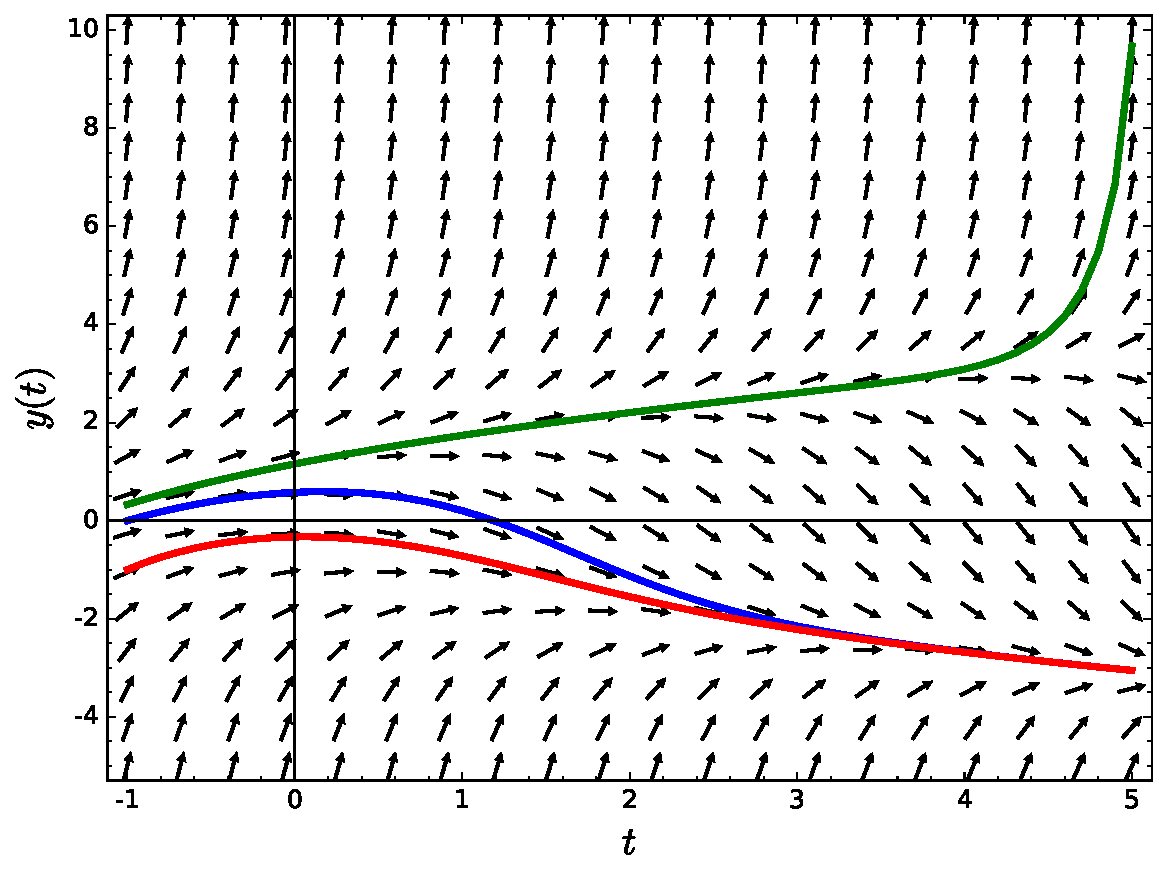
\includegraphics[width=\linewidth]{generated/sageplot/firstlook03-direction-field.pdf}%
\end{image}%
\tcblower
\end{figureptx}%
Although direction fields can be tedious to compute using pencil and paper, we can easily generate direction fields for any differential equation with the use of computer software. Most computer algebra systems, including \emph{Sage}, have facilities for generating and graphing direction fields. For example, the following \emph{Sage} cell will generate the direction field for \(y' = y^2/2 - t\) using the command \mono{plot\_slope\_field}. We will learn how to add solution curves at the end of this section.%
\begin{sageinput}
t, y = var('t, y')
f(t, y) = y^2/2 - t
plot_slope_field(f, (t, -1, 5), (y, -5, 10), headaxislength=3, headlength=3, axes_labels=['$t$','$y(t)$'])
\end{sageinput}
\begin{activity}{Plotting Direction Fields.}{g:activity:idp105545991797008}%
Plot the direction field and the solution curves for each of the following initial conditions.%
\begin{enumerate}[font=\bfseries,label=(\alph*),ref=\alph*]
\item{}\(y' = y - 2x\), \(y(0) = 4\), \(y(0) = 1\).%
\item{}\(y' = y(1 + x)\), \(y(0) = 1\), \(y(0) = 0\), \(y(0) = -1\).%
\item{}\(\dfrac{dx}{dt} + 2tx = x\), \(x(0) = 5\).%
\item{}\(\dfrac{dy}{dt} = 2y(1 - y/4)\), \(y(0) = 1\), \(y(0) = 4\), \(y(0) = 5\).%
\item{}\(y' = -1 - y^4\), \(y(0) = 4\), \(y(0) = 0\), \(y(0) = -4\).%
\end{enumerate}
In each case comment on anything that you notice about the direction field and the solutions.%
\end{activity}%
\end{subsectionptx}
%
%
\typeout{************************************************}
\typeout{Subsection 1.3.3 RC Circuits Revisited}
\typeout{************************************************}
%
\begin{subsectionptx}{RC Circuits Revisited}{}{RC Circuits Revisited}{}{}{x:subsection:firstlook03-subsection-rc-circuits-revisited}
Now let us return to our RC circuit and consider different functions \(E(t)\) for the differential equation%
\begin{equation*}
\frac{d E_C}{dt} = \frac{E(t) - E_C}{RC},
\end{equation*}
with \(R = 1\) and \(C = 1\). First suppose that there is no voltage source in the circuit. If we let \(E(t) = 0\) for all \(t \ge 0\), we will get the direction field of given in \hyperref[x:figure:firstlook03-figure-no-current]{Figure~{\xreffont\ref{x:figure:firstlook03-figure-no-current}}}. The direction field agrees with our analytic solution%
\begin{equation*}
E_C(t) = v_0 e^{-t},
\end{equation*}
where \(v_0 = E_C(0)\).%
\begin{figureptx}{The direction field for no current}{x:figure:firstlook03-figure-no-current}{}%
\begin{image}{0.2}{0.6}{0.2}%
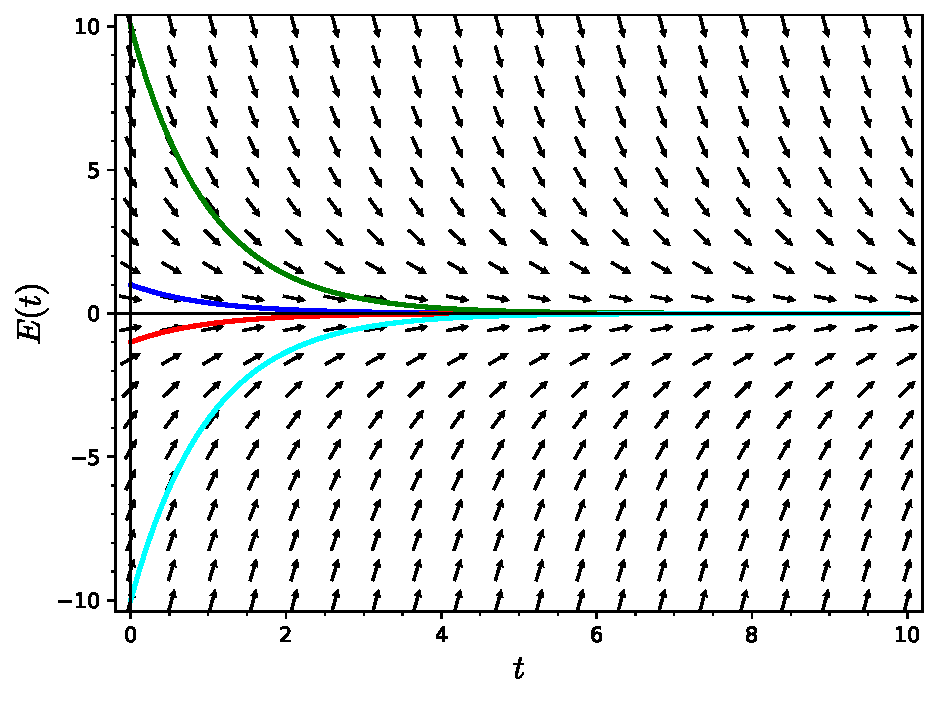
\includegraphics[width=\linewidth]{generated/sageplot/firstlook03-no-current.pdf}%
\end{image}%
\tcblower
\end{figureptx}%
If we assume that we have a nonzero constant source of voltage, \(E(t) = K\), in our circuit such as a battery, then we obtain the separable differential equation%
\begin{equation*}
\frac{d E_C}{dt} = K - E_C.
\end{equation*}
The direction field for this differential equation for \(K = 10\) is given in \hyperref[x:figure:firstlook03-figure-constant-current]{Figure~{\xreffont\ref{x:figure:firstlook03-figure-constant-current}}}.%
\begin{figureptx}{The direction field for a constant current}{x:figure:firstlook03-figure-constant-current}{}%
\begin{image}{0.2}{0.6}{0.2}%
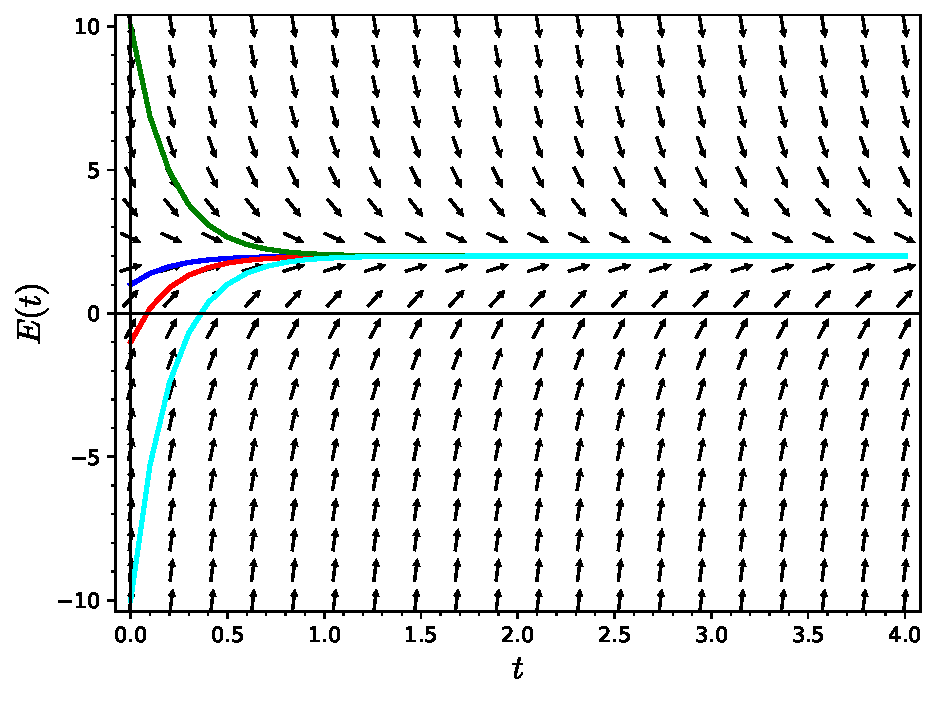
\includegraphics[width=\linewidth]{generated/sageplot/firstlook03-constant-current.pdf}%
\end{image}%
\tcblower
\end{figureptx}%
If we attach a battery to our circuit at time \(t = 0\) and then disconnect the battery at \(t = 4\), then we obtain a different solution. For example, if%
\begin{equation*}
E(t) =
\begin{cases}
10     & 0 \leq t \leq 4, \\
0     & t \gt 4,
\end{cases}
\end{equation*}
we will obtain a different direction field (\hyperref[x:figure:firstlook03-figure-single-pulse]{Figure~{\xreffont\ref{x:figure:firstlook03-figure-single-pulse}}}).%
\begin{figureptx}{The direction field for a single pulse}{x:figure:firstlook03-figure-single-pulse}{}%
a direction field of slope arrows and three curves following the arrows with the curves approaching ten and then to zero once the time is four\begin{image}{0.2}{0.6}{0.2}%
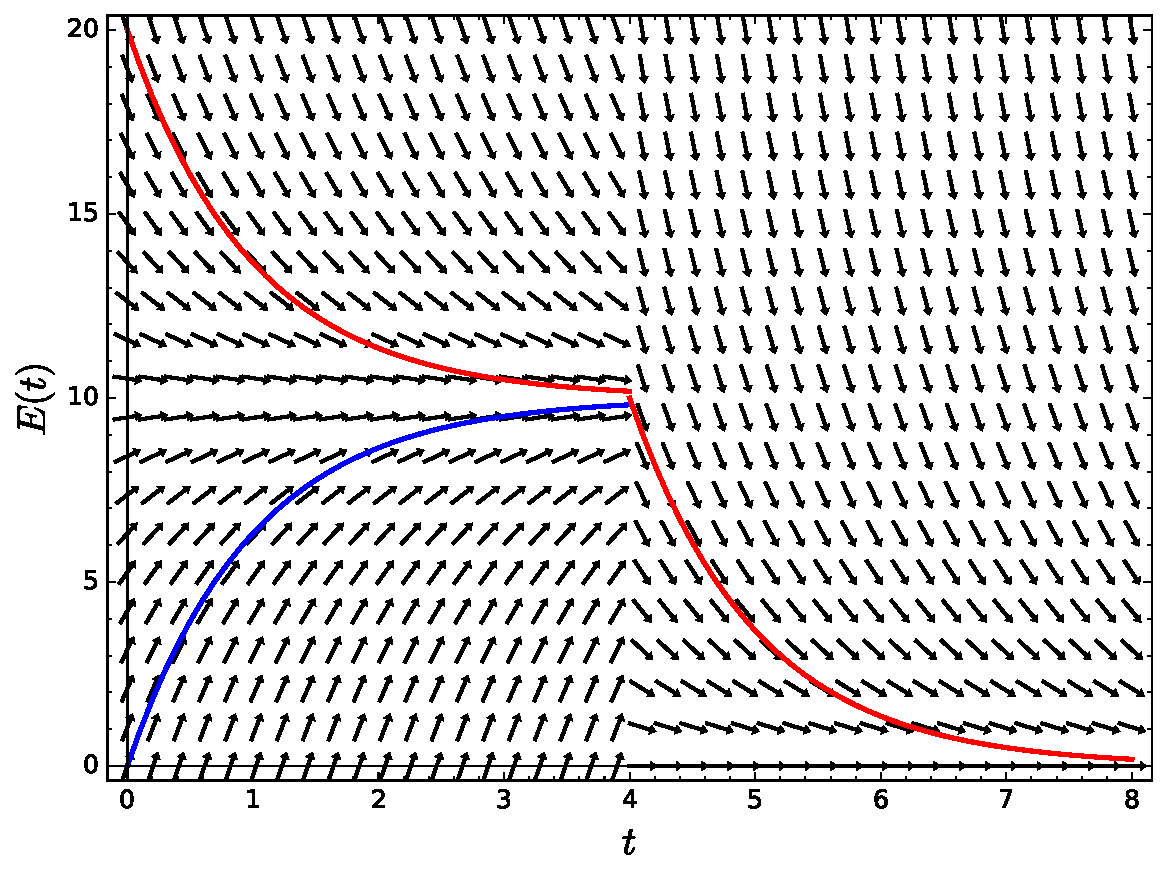
\includegraphics[width=\linewidth]{generated/sageplot/firstlook03-single-pulse-current.pdf}%
\end{image}%
\tcblower
\end{figureptx}%
If our voltage source emits a series of pulses, say%
\begin{equation*}
E(t) =
\begin{cases}
10 & 0 \leq t \lt 4, \\
0 & 4 \leq t \lt 8, \\
10 & 8 \leq t \lt 12, \\
& \vdots
\end{cases}
\end{equation*}
then the direction field for our differential equation is given in \hyperref[x:figure:firstlook03-figure-series-pulses]{Figure~{\xreffont\ref{x:figure:firstlook03-figure-series-pulses}}}.%
\begin{figureptx}{The direction field for a series of pulses}{x:figure:firstlook03-figure-series-pulses}{}%
\begin{image}{0.2}{0.6}{0.2}%
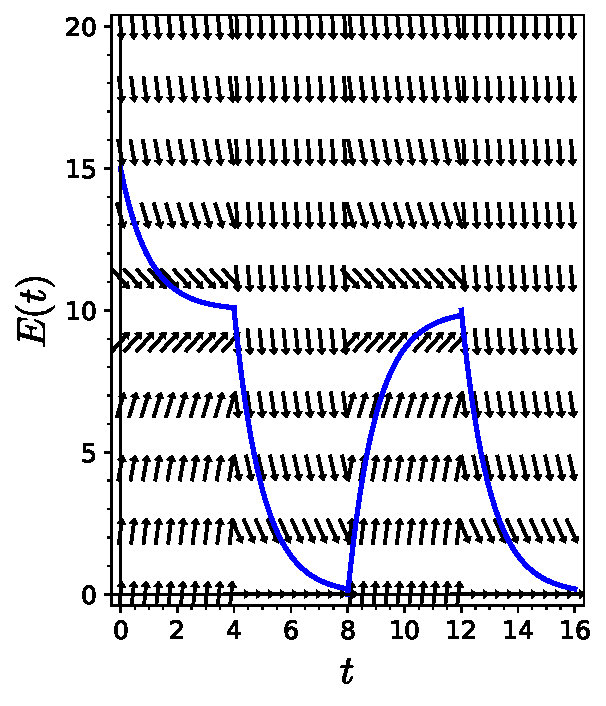
\includegraphics[width=\linewidth]{generated/sageplot/firstlook03-series-pulses.pdf}%
\end{image}%
\tcblower
\end{figureptx}%
Finally, if we use a generator for a voltage source, the voltage source might be given by a function such as \(E(t) = \sin(\pi t /2)\). The direction field for this circuit is given in \hyperref[x:figure:firstlook03-figure-oscillating-voltage]{Figure~{\xreffont\ref{x:figure:firstlook03-figure-oscillating-voltage}}}.%
\begin{figureptx}{The direction field for an oscillating voltage}{x:figure:firstlook03-figure-oscillating-voltage}{}%
\begin{image}{0.2}{0.6}{0.2}%
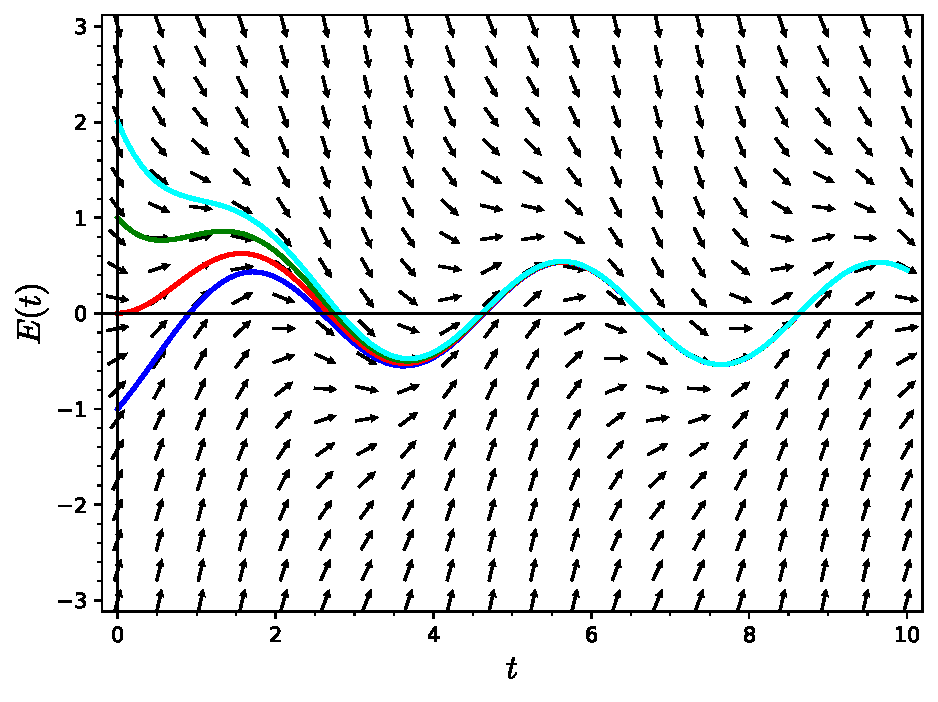
\includegraphics[width=\linewidth]{generated/sageplot/firstlook03-oscillating-voltage.pdf}%
\end{image}%
\tcblower
\end{figureptx}%
\end{subsectionptx}
%
%
\typeout{************************************************}
\typeout{Subsection 1.3.4 Plotting Direction Fields with Sage}
\typeout{************************************************}
%
\begin{subsectionptx}{Plotting Direction Fields with Sage}{}{Plotting Direction Fields with Sage}{}{}{x:subsection:firstlook03-subsection-sage-direction-fields}
The Sage interact below will help you plot direction fields for a given initial value problem. A Sage interact is a menu driven Sage applet. All of the Sage code is ``under the hood.'' You can then change each field in the cell output to solve a particular initial value problem.%
\begin{figureptx}{A Sage applet for plotting direction fields}{x:figure:firstlook03-figure-interactive-direction-fields}{}%
\centering
\setlength{\qrsize}{9em}
\setlength{\previewwidth}{\linewidth}
\addtolength{\previewwidth}{-\qrsize}
\begin{tcbraster}[raster columns=2, raster column skip=1pt, raster halign=center, raster force size=false, raster left skip=0pt, raster right skip=0pt]%
\begin{tcolorbox}[previewstyle, width=\previewwidth]%
\IfFileExists{generated/preview/firstlook03-interactive-direction-fields-preview.png}%
{\includegraphics[width=0.80\linewidth,height=\qrsize,keepaspectratio]{generated/preview/firstlook03-interactive-direction-fields-preview.png}}%
{\small{}Specify a static image with the \mono{@preview} attribute;\\%
Or create and provide an automatic screenshot as\\%
\mono{generated/preview/firstlook03-interactive-direction-fields-preview.png}\\%
via the \mono{PreTeXt-CLI} application or \mono{pretext/pretext} script.}%
\end{tcolorbox}%
\begin{tcolorbox}[qrstyle]%
{\hypersetup{urlcolor=black}\qrcode[height=\qrsize]{firstlook03-interactive-direction-fields.html}}%
\end{tcolorbox}%
\end{tcbraster}%
\tcblower
\end{figureptx}%
Of course, it is quite easy to give the interact an initial value problem that yield unitelligible results.%
\end{subsectionptx}
%
%
\typeout{************************************************}
\typeout{Subsection 1.3.5 Autonomous Differential Equations}
\typeout{************************************************}
%
\begin{subsectionptx}{Autonomous Differential Equations}{}{Autonomous Differential Equations}{}{}{x:subsection:firstlook03-subsection-autonomous-equations}
An \terminology{autonomous differential equation}\index{differential equation!autonomous} is one of the form%
\begin{equation*}
\frac{dx}{dt} = f(x).
\end{equation*}
In other words, a differential equation is autonomous if the variable \(t\) does not appear on the righthand side of the equation. Since an autonomous differential equation \(dx/dt = f(x)\) only depends on the variable \(x\), its direction field is particularly easy to graph. The slope only depends on \(x\) and is the same for all values of \(t\).%
\begin{example}{A Logistic Model with Harvesting.}{x:example:firstlook03-example-harvesting}%
Let us consider a trout pond that has a carrying capacity of 200 fish. Suppose that the trout population can be modeled according to the logistic equation\index{harvesting}%
\begin{equation*}
\frac{dP}{dt} = P\left(1 - \frac{P}{200} \right),
\end{equation*}
where \(t\) is the time in years. If we allow the fish to be harvested at a constant rate of 32 per year, our equation becomes%
\begin{equation*}
\frac{dP}{dt} = P\left(1 - \frac{P}{200} \right) - 32.
\end{equation*}
The direction field for this equation is given in \hyperref[x:figure:firstlook03-figure-logistic-direction-field]{Figure~{\xreffont\ref{x:figure:firstlook03-figure-logistic-direction-field}}}.%
\begin{figureptx}{Logistic growth with harvesting}{x:figure:firstlook03-figure-logistic-direction-field}{}%
\begin{image}{0.2}{0.6}{0.2}%
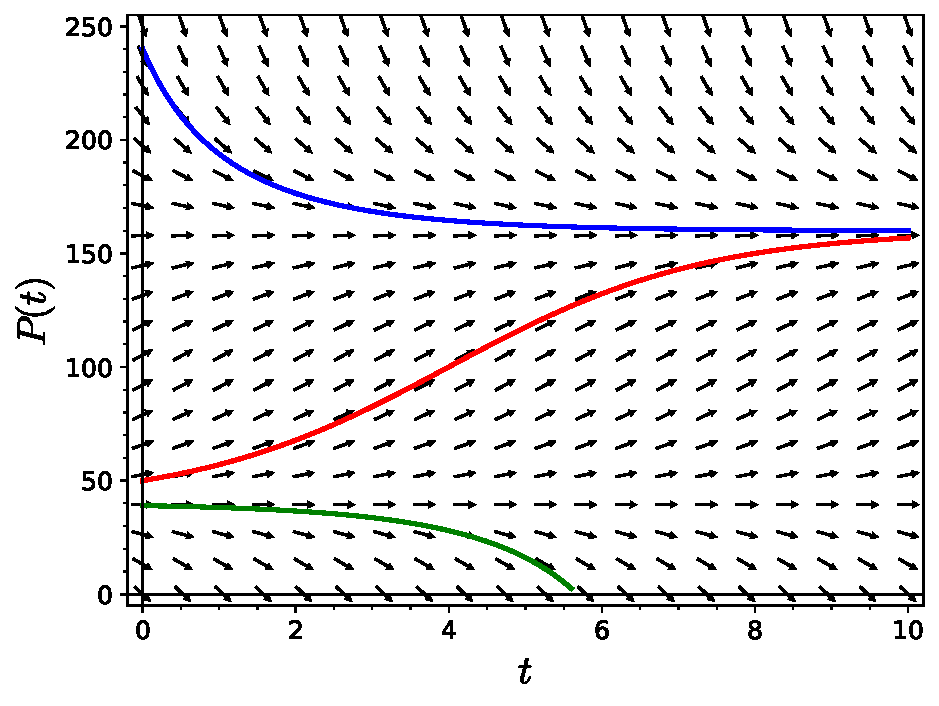
\includegraphics[width=\linewidth]{generated/sageplot/firstlook03-logistic-direction-field.pdf}%
\end{image}%
\tcblower
\end{figureptx}%
One of the basic questions that we can ask of our model is whether or not we have a sustainable population in our trout pond given this harvest rate. If so, under what conditions for sustainablility?%
\end{example}
Since%
\begin{equation*}
\frac{dP}{dt} = P\left(1 - \frac{P}{200} \right) - 32 = -\frac{1}{200}(P - 40)(P - 160)
\end{equation*}
is an autonomous differential equation, the direction field does not depend on \(t\). Consequently, we need only keep track of what happens on the vertical axis.  We can do this with a \terminology{phase line}\index{phase line}.  Instead of drawing the entire direction field, we can draw a single line containing the same information (\hyperref[x:figure:firstlook03-figure-phase-line]{Figure~{\xreffont\ref{x:figure:firstlook03-figure-phase-line}}}).%
\begin{figureptx}{Phase line diagram}{x:figure:firstlook03-figure-phase-line}{}%
\begin{image}{0.3}{0.4}{0.3}%
\resizebox{\linewidth}{!}{%
                    \begin{tikzpicture}[scale=0.4]
\draw[thick] (0,-1) -- (0,11);
\filldraw (0,8) node[right] {$P = 160$ is a sink} circle (0.2);
\filldraw (0,2) node[right] {$P = 40$ is a source} circle (0.2);
\filldraw (0,10) -- (-0.2, 10.4) -- (0.2, 10.4) -- cycle;
\filldraw (0,0) -- (-0.2, 0.4) -- (0.2, 0.4) -- cycle;
\filldraw (0,5.4) -- (-0.2, 5) -- (0.2, 5) -- cycle;
\end{tikzpicture}
}%
\end{image}%
\tcblower
\end{figureptx}%
Notice that \(dP/dt = 0\) when \(P= 40\) or \(P = 160\). Thus, the two constant solutions \(P(t) = 40\) and \(P(t) = 160\) are the same for all values of the independent variable \(t\). We say that such a solution is an \terminology{equilibrium solution}\index{equilibrium solution}. Equilibrium solutions graph as horizontal lines on the direction field. We can identify equilibrium solutions by setting the derivative of the function equal to zero. On our phase line we will represent these solutions as equilibrium points. For values of \(P\) between 40 and 160, we know that \(dP/dt \gt 0\). Thus, any solution curve must be increasing. We denote this property on the phase line by drawing an upward pointing arrow. On the other hand, we know that \(dP/dt \lt 0\) when \(P \lt 40\) or \(P \gt 160\). In this case any solution curve will be decreasing, and we will indicate this by a downward pointing arrow.%
\par
Let \(y' = f(y)\) and suppose that \(y = y_0\) is an equilibrium solution. We say this solution is a \terminology{sink}\index{equilibrium solution!sink} if for any solution \(y(t)\) with initial condition sufficiently close to \(y_0\), we have%
\begin{equation*}
\lim_{t \to \infty} y(t) = y_0.
\end{equation*}
We say that an equilibrium point is a \terminology{source}\index{equilibrium solution!source} if all solutions that start sufficiently close to \(y_0\) tend toward \(y_0\) as \(t \to - \infty\). An equilibrium solution that is neither a sink or a source is called a \terminology{node}\index{equilibrium solution!node} (\hyperref[x:figure:firstlook03-figure-phase-line]{Figure~{\xreffont\ref{x:figure:firstlook03-figure-phase-line}}}). When \(P= 40\), we have a source, and when \(P = 160\), we have a sink.%
\par
An equilibrium solution is \terminology{stable}\index{equilibrium solution!stable} if a small change in the initial conditions gives a solution which tends toward the equilibrium as the independent variable tends towards positive infinity. An equilibrium solution is \terminology{unstable}\index{equilibrium solution!unstable} if a small change in the initial conditions gives a solution which veers away from the equilibrium as the independent variable tends towards positive infinity.%
\par
Consider the differential equation%
\begin{equation}
\frac{dy}{dt} = y^4 - 4y^2 = y^2(y + 2)(y - 2).\label{x:men:firstlook03-equation-sinks-sources-nodes}
\end{equation}
The graph of \(f(y) = y^4 - 4y^2\) is given in \hyperref[x:figure:firstlook03-figure-sinks-sources-nodes]{Figure~{\xreffont\ref{x:figure:firstlook03-figure-sinks-sources-nodes}}}. If \(y = -2\), we have a sink.  If \(y = 2\), we have a source.  Finally, if \(y = 0\), we have a node.%
\begin{figureptx}{Sinks, sources, and nodes}{x:figure:firstlook03-figure-sinks-sources-nodes}{}%
\begin{image}{0.2}{0.6}{0.2}%
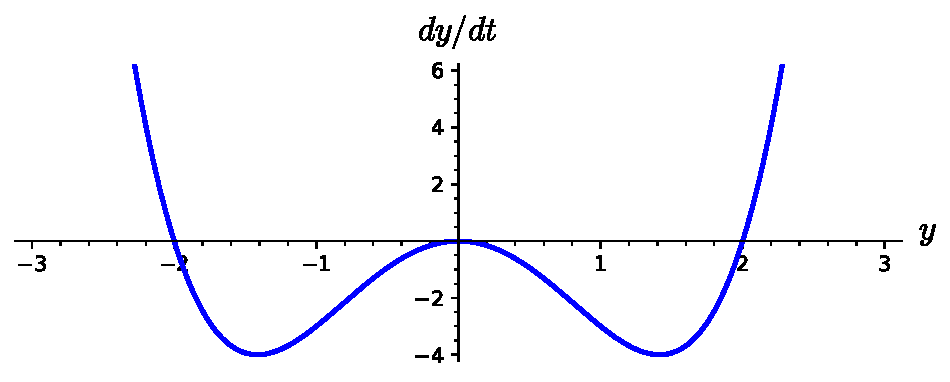
\includegraphics[width=\linewidth]{generated/sageplot/firstlook03-sinks-sources-nodes.pdf}%
\end{image}%
\tcblower
\end{figureptx}%
It is easy to generate a phase line diagram for equation~\hyperref[x:men:firstlook03-equation-sinks-sources-nodes]{({\xreffont\ref{x:men:firstlook03-equation-sinks-sources-nodes}})} from the graph of \(f(y) = y^2(y + 2)(y - 2)\) (\hyperref[x:figure:firstlook03-figure-sinks-sources-nodes]{Figure~{\xreffont\ref{x:figure:firstlook03-figure-sinks-sources-nodes}}}). If the graph is above the \(y\)-axis, then \(y\) is increasing. If the graph is below the \(y\)-axis, then \(y\) is decreasing. Therefore, the phase line is easy to sketch (\hyperref[x:figure:firstlook03-figure-phase-line-1]{Figure~{\xreffont\ref{x:figure:firstlook03-figure-phase-line-1}}}).%
\begin{figureptx}{Phase line diagram for \(y' = y^2(y + 2)(y - 2)\)}{x:figure:firstlook03-figure-phase-line-1}{}%
\begin{image}{0.35}{0.3}{0.35}%
\resizebox{\linewidth}{!}{%
                    \begin{tikzpicture}[scale=1]
\draw[thick] (0,-3.5) -- (0,3.5);
\filldraw (0,0) node[right] {$y = 0$ is a node} circle (0.05);
\filldraw (0,2) node[right] {$y = 2$ is a source} circle (0.05);
\filldraw (0,-2) node[right] {$y = -2$ is a sink} circle (0.05);
\filldraw (0,1) -- (-0.1, 1.2) -- (0.1, 1.2) -- cycle;
 \filldraw (0,-1) -- (-0.1, -0.8) -- (0.1, -0.8) -- cycle;
\filldraw (0,-2.6) -- (-0.1, -2.8) -- (0.1, -2.8) -- cycle;
 \filldraw (0,2.8) -- (-0.1, 2.6) -- (0.1, 2.6) -- cycle;
\end{tikzpicture}
}%
\end{image}%
\tcblower
\end{figureptx}%
\begin{activity}{Autonomous Equations and Phase Lines.}{g:activity:idp105545991602576}%
For each of the differential equations below, draw the phase line and classify each equilibrium solution as a sink, a source, or a node.%
\begin{enumerate}[font=\bfseries,label=(\alph*),ref=\alph*]
\item{}\(y' = y(y - 2)(y + 3)\).%
\item{}\(y' = y^2(y - 2)(y + 3)\).%
\item{}\(y' = \cos y\).%
\item{}\(y' = \cos^2 y\).%
\end{enumerate}
In each case comment on anything that you notice about the phase line and the equilibrium solutions.%
\end{activity}%
One of the reasons why autonomous equations are so important is Taylor's theorem, which tells us that any function \(f(x)\) can be approximated near a point \(x_0\) by an \(n\)th degree polynomial,%
\begin{equation*}
f(x) \approx f(x_0) + f'(x_0)(x - x_0) + \frac{ f''(x_0)}{2!} (x - x_0)^2 + \cdots + \frac{ f^{(n)}(x_0)}{n!} (x - x_0)^n
\end{equation*}
near \(x_0\).  For example, if%
\begin{equation*}
\frac{dx}{dt} = f(x) = \cos(x^2 + \pi)
\end{equation*}
with \(x(0) = x_0\), then we may approximate this initial value problem near \(x_0\) with%
\begin{align*}
\frac{dx}{dt} & =  f(x_0) + f'(x_0)(x - x_0) = \cos(x_0^2 + \pi) + 2 x _0 \sin(x_0^2 + \pi)(x - x_0)\\
x(0) & = x_0.
\end{align*}
Of course, this strategy might not work very well if \(f(x_0) = \cos(x_0^2 + \pi) = 0\) or \(f'(x_0) = 2 x _0 \sin(x_0^2 + \pi) = 0\).%
\end{subsectionptx}
%
%
\typeout{************************************************}
\typeout{Subsection 1.3.6 Important Lessons}
\typeout{************************************************}
%
\begin{subsectionptx}{Important Lessons}{}{Important Lessons}{}{}{x:subsection:firstlook03-subsection-important-lessons}
%
\begin{itemize}[label=\textbullet]
\item{}Direction fields and phase lines are a useful way of analyzing a differential equation from a geometric point of view, especially since not all differential equations can be solved analytically.%
\item{}An autonomous equation is a differential equation of the form \(y' = f(y)\).  We can use a phase line to analyze autonomous differential equations.%
\item{}Equilibrium solutions to a differential equation \(y' = f(y)\) are those solutions given by \(f(y) = 0\) for all \(y\).  In this case, any solution must be constant.  We can classify equilibrium solutions according to whether they are stable or unstable.  In particular, an equilibrium solution is either a sink, source, or node.%
\end{itemize}
%
\end{subsectionptx}
%
%
\typeout{************************************************}
\typeout{Reading Questions 1.3.7 Reading Questions}
\typeout{************************************************}
%
\begin{reading-questions-subsection}{Reading Questions}{}{Reading Questions}{}{}{x:reading-questions:reading-questions-firstlook03}
\begin{divisionexercise}{1}{}{}{x:exercise:reading-questions-firstlook03-1}%
Explain why solution curves to a differential equation cannot intersect.%
\end{divisionexercise}%
\begin{divisionexercise}{2}{}{}{x:exercise:reading-questions-firstlook03-2}%
Explain in your own words what an autonomous differential equation is.%
\end{divisionexercise}%
\end{reading-questions-subsection}
%
%
\typeout{************************************************}
\typeout{Exercises 1.3.8 Exercises}
\typeout{************************************************}
%
\begin{exercises-subsection}{Exercises}{}{Exercises}{}{}{x:exercises:firstlook03-exercises}
\par\medskip\noindent%
\textbf{Plotting direction fields by hand.}\space\space\hypertarget{x:exercisegroup:firstlook03-exercises-sketching-direction-fields}{}%
For each of the differential equations in \hyperlink{x:exercisegroup:firstlook03-exercises-sketching-direction-fields}{Exercise Group~{\xreffont 1.3.8.1\textendash{}6}}, plot the direction field on the integer coordinates \((t,x)\) of the rectangle \(-2 \lt t \lt 2\) and \(-2 \lt x \lt 2\) by drawing a short line of the appropriate slope.%
\begin{exercisegroupcol}{2}
\begin{divisionexerciseegcol}{1}{}{}{x:exercise:firstlook03-exercise-sketching-direction-field-1}%
\(x' = x + t\)%
\end{divisionexerciseegcol}%
\begin{divisionexerciseegcol}{2}{}{}{x:exercise:firstlook03-exercise-sketching-direction-field-2}%
\(x' = xt\)%
\end{divisionexerciseegcol}%
\begin{divisionexerciseegcol}{3}{}{}{x:exercise:firstlook03-exercise-sketching-direction-field-3}%
\(x' = x^2 + t^2\)%
\end{divisionexerciseegcol}%
\begin{divisionexerciseegcol}{4}{}{}{x:exercise:firstlook03-exercise-sketching-direction-field-4}%
\(x' = t + \tan(x)\)%
\end{divisionexerciseegcol}%
\begin{divisionexerciseegcol}{5}{}{}{x:exercise:firstlook03-exercise-sketching-direction-field-5}%
\(x' = (x + t)/(x^2 + t^2)\)%
\end{divisionexerciseegcol}%
\begin{divisionexerciseegcol}{6}{}{}{x:exercise:firstlook03-exercise-sketching-direction-field-6}%
\(x' = x - t + 1\)%
\end{divisionexerciseegcol}%
\end{exercisegroupcol}
\par\medskip\noindent
\begin{divisionexercise}{7}{}{}{x:exercise:firstlook03-exercise-sketching-direction-field-w-sage}%
Use Sage to plot the direction fields of each differential equation in \hyperlink{x:exercisegroup:firstlook03-exercises-sketching-direction-fields}{Exercise Group~{\xreffont 1.3.8.1\textendash{}6}}.%
\begin{sageinput}
t, x = var('t, x')
f(t,x) = x + t
plot_slope_field(f, (t, -2, 2), (x, -2, 2), headaxislength=3, headlength=3, axes_labels=['$t$','$x(t)$'])
\end{sageinput}
\begin{sageoutput}

\end{sageoutput}
\end{divisionexercise}%
\par\medskip\noindent%
\textbf{Equilibrium solutions and phase lines.}\space\space\hypertarget{x:exercisegroup:firstlook03-exercises-phaselines}{}%
Find the equilibrium solutions for each of the differential equations in \hyperlink{x:exercisegroup:firstlook03-exercises-phaselines}{Exercise Group~{\xreffont 1.3.8.8\textendash{}13}}. Draw the phase line for each equation and classify each equilibrium solution as a sink, a source, or a node.%
\begin{exercisegroupcol}{2}
\begin{divisionexerciseegcol}{8}{}{}{x:exercise:firstlook03-exercise-phaseline-1}%
\(y' = 2y - 5\)%
\end{divisionexerciseegcol}%
\begin{divisionexerciseegcol}{9}{}{}{x:exercise:firstlook03-exercise-phaseline-2}%
\(\dfrac{dx}{dt} = (x - 1)(x + 2)\)%
\end{divisionexerciseegcol}%
\begin{divisionexerciseegcol}{10}{}{}{x:exercise:firstlook03-exercise-phaseline-3}%
\(\dfrac{dx}{dt} = (x^2 - 1)(x - 2)\)%
\end{divisionexerciseegcol}%
\begin{divisionexerciseegcol}{11}{}{}{x:exercise:firstlook03-exercise-phaseline-4}%
\(\dfrac{dy}{dx} = \sin 2y\)%
\end{divisionexerciseegcol}%
\begin{divisionexerciseegcol}{12}{}{}{x:exercise:firstlook03-exercise-phaseline-5}%
\(x' = (x^2 + 1)(x - 1)\)%
\end{divisionexerciseegcol}%
\begin{divisionexerciseegcol}{13}{}{}{x:exercise:firstlook03-exercise-phaseline-6}%
\(x' = x^2 + x + 1\)%
\end{divisionexerciseegcol}%
\end{exercisegroupcol}
\par\medskip\noindent
\par\medskip\noindent%
\textbf{Sketching solutions.}\space\space\hypertarget{x:exercisegroup:firstlook03-exercises-sketching-solutions}{}%
Each of the differential equations in \hyperlink{x:exercisegroup:firstlook03-exercises-sketching-solutions}{Exercise Group~{\xreffont 1.3.8.14\textendash{}19}} has several initial conditions specified. Sketch the solution curves that satisfy the initial conditions.  Sketch your solutions for each equation on the same pair of axes.%
\begin{exercisegroup}
\begin{divisionexerciseeg}{14}{}{}{x:exercise:firstlook03-exercise-sketching-solution-1}%
\(y' = 2y - 5\), \(y(0) = 4\), \(y(0) = 2\), \(y(0) = 0\).%
\end{divisionexerciseeg}%
\begin{divisionexerciseeg}{15}{}{}{x:exercise:firstlook03-exercise-sketching-solution-2}%
\(\dfrac{dx}{dt} = (x - 1)(x + 2)\), \(x(0) = 2\), \(x(0) = 1\), \(x(0) = 0\).%
\end{divisionexerciseeg}%
\begin{divisionexerciseeg}{16}{}{}{x:exercise:firstlook03-exercise-sketching-solution-3}%
\(\dfrac{dx}{dt} = (x^2 - 1)(x - 2)\), \(x(0) = 1\), \(x(0) = 0\), \(x(0) = -1\).%
\end{divisionexerciseeg}%
\begin{divisionexerciseeg}{17}{}{}{x:exercise:firstlook03-exercise-sketching-solution-4}%
\(\dfrac{dy}{dx} = \sin 2y\), \(y(0) = 2\), \(y(0) = 1\), \(y(0) = 0\).%
\end{divisionexerciseeg}%
\begin{divisionexerciseeg}{18}{}{}{x:exercise:firstlook03-exercise-sketching-solution-5}%
\(x' = (x^2 + 1)(x - 1)\), \(x(0) = 2\), \(x(0) = 1\), \(x(0) = 0\).%
\end{divisionexerciseeg}%
\begin{divisionexerciseeg}{19}{}{}{x:exercise:firstlook03-exercise-sketching-solution-6}%
\(x' = x^2 + x + 1\), \(x(0) = 1\), \(x(0) = 0\), \(x(0) = -1\).%
\end{divisionexerciseeg}%
\end{exercisegroup}
\par\medskip\noindent
\par\medskip\noindent%
\textbf{Phase lines from graphs of the derivative.}\space\space\hypertarget{x:exercisegroup:firstlook03-exercises-derivative-graphs}{}%
Consider the differential equation \(y' = f(y)\), where the graph of \(f(y)\) is given in \hyperlink{x:exercisegroup:firstlook03-exercises-derivative-graphs}{Exercise Group~{\xreffont 1.3.8.20\textendash{}23}}. Draw the phase line for each equation and classify each equilibrium solution as a sink, a source, or a node.%
\begin{exercisegroupcol}{2}
\begin{divisionexerciseegcol}{20}{}{}{g:exercise:idp105545991681808}%
\begin{image}{0}{1}{0}%
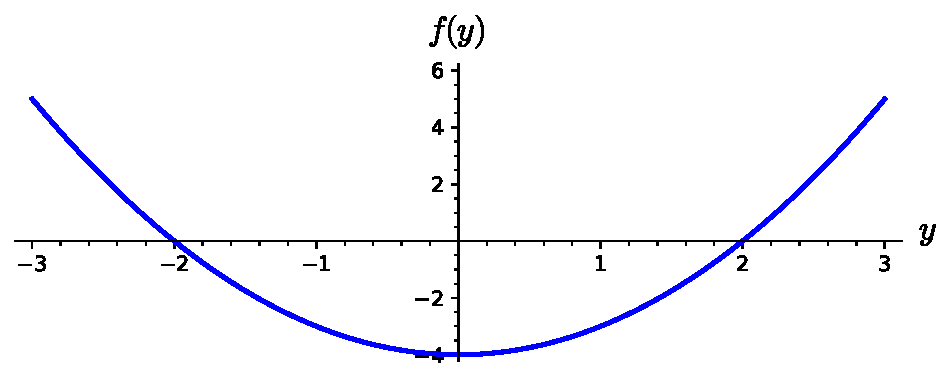
\includegraphics[width=\linewidth]{generated/sageplot/firstlook03-exercise-derivative-graphs-1.pdf}%
\end{image}%
\end{divisionexerciseegcol}%
\begin{divisionexerciseegcol}{21}{}{}{g:exercise:idp105545991683216}%
\begin{image}{0}{1}{0}%
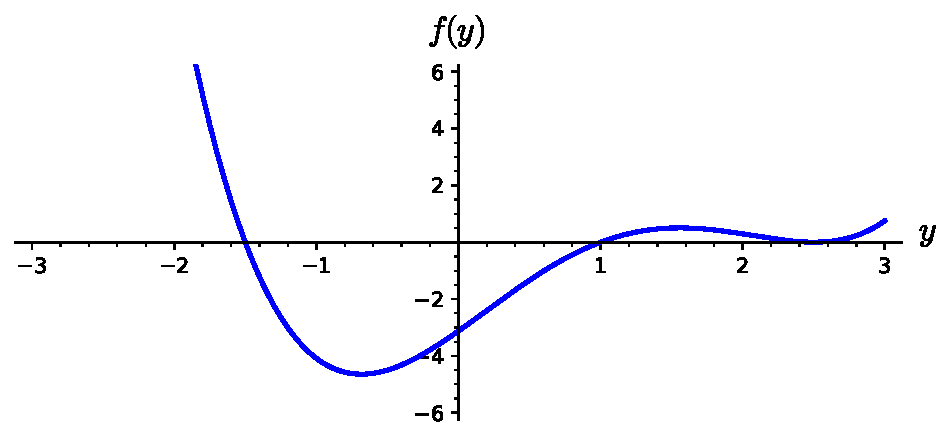
\includegraphics[width=\linewidth]{generated/sageplot/firstlook03-exercise-derivative-graphs-2.pdf}%
\end{image}%
\end{divisionexerciseegcol}%
\begin{divisionexerciseegcol}{22}{}{}{g:exercise:idp105545991684624}%
\begin{image}{0}{1}{0}%
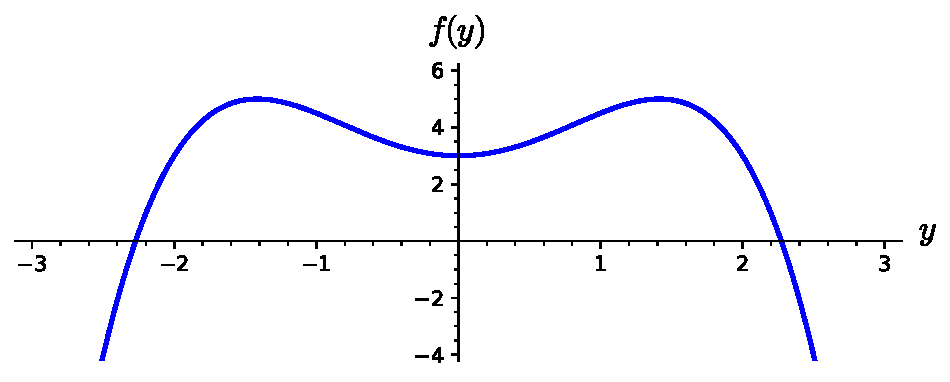
\includegraphics[width=\linewidth]{generated/sageplot/firstlook03-exercise-derivative-graphs-3.pdf}%
\end{image}%
\end{divisionexerciseegcol}%
\begin{divisionexerciseegcol}{23}{}{}{g:exercise:idp105545991686032}%
\begin{image}{0}{1}{0}%
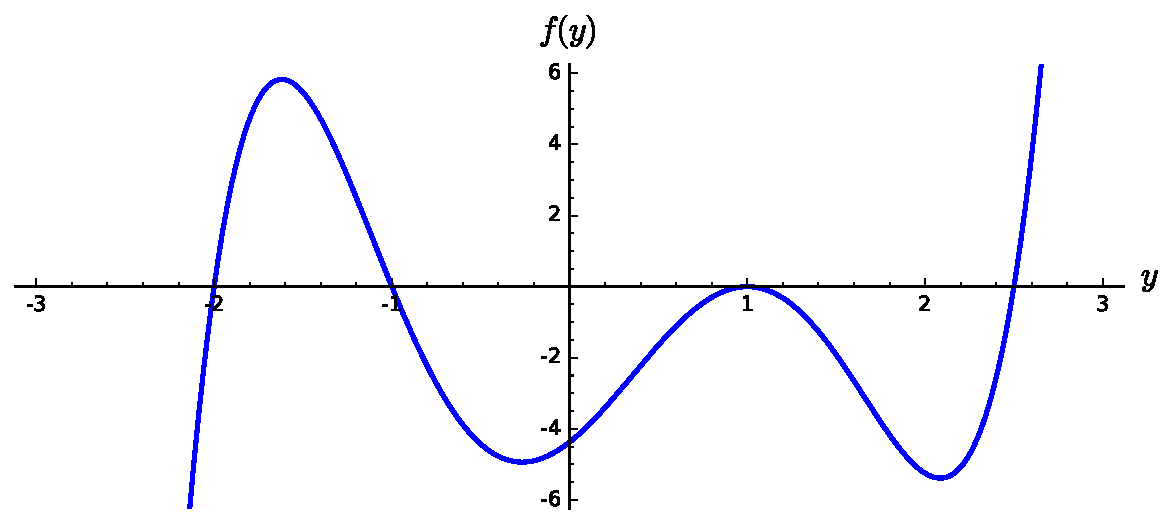
\includegraphics[width=\linewidth]{generated/sageplot/firstlook03-exercise-derivative-graphs-4.pdf}%
\end{image}%
\end{divisionexerciseegcol}%
\end{exercisegroupcol}
\par\medskip\noindent
\begin{divisionexercise}{24}{}{}{g:exercise:idp105545991687440}%
What happens if we increase the harvest rate to 100 in \hyperref[x:example:firstlook03-example-harvesting]{Example~{\xreffont\ref{x:example:firstlook03-example-harvesting}}}? What should be our strategy to maintain a viable population in the trout pond and still permit fishing?%
\end{divisionexercise}%
\end{exercises-subsection}
%
%
\typeout{************************************************}
\typeout{Subsection 1.3.9 Sage\textemdash{}Plotting Direction Fields and Solutions}
\typeout{************************************************}
%
\begin{subsectionptx}{Sage\textemdash{}Plotting Direction Fields and Solutions}{}{Sage\textemdash{}Plotting Direction Fields and Solutions}{}{}{x:subsection:firstlook03-subsection-sage}
%
%
\typeout{************************************************}
\typeout{Subsubsection 1.3.9.1 Plotting direction fields}
\typeout{************************************************}
%
\begin{subsubsectionptx}{Plotting direction fields}{}{Plotting direction fields}{}{}{x:subsubsection:firstlook03-subsection-direction-fields-sage}
If we wish to plot a direction field for a differential equation, we can use the command \mono{plot\_slope\_field}. Let us plot the direction field for the equation \(y' = y^2/2 - t\).%
\begin{sageinput}
t, y = var('t, y')
f(t, y) = y^2/2 - t
v = plot_slope_field(f, (t,-1,5), (y,-5,10), headaxislength=3, headlength=3, axes_labels=['$t$','$y(t)$'])
v
\end{sageinput}
\begin{sageoutput}

\end{sageoutput}
There are a few extra commands to specify the size of the arrows in the plot and to label the axes. Try changing or omitting these commands and see what happens.%
\begin{sageinput}
t, y = var('t, y')
f(t, y) = y^2/2 - t
v = plot_slope_field(f, (t,-1,5), (y,-5,10), headaxislength=3, headlength=3, axes_labels=['$t$','$y(t)$'])
v
\end{sageinput}
\begin{sageoutput}

\end{sageoutput}
For more examples and options, see \href{http://doc.sagemath.org/html/en/reference/plotting/sage/plot/plot_field.html}{\nolinkurl{doc.sagemath.org/html/en/reference/plotting/sage/plot/plot_field.html}}%
\end{subsubsectionptx}
%
%
\typeout{************************************************}
\typeout{Subsubsection 1.3.9.2 Plotting solutions}
\typeout{************************************************}
%
\begin{subsubsectionptx}{Plotting solutions}{}{Plotting solutions}{}{}{x:subsubsection:firstlook03-subsection-desolve_rk4}
Now let us find a numerical solution to the equation using the command \mono{desolve\_rk4}. This is a fourth-order Runge-Kutta method, and returns a numerical solution (a table of values). Here, we must supply the dependent variable and initial conditions.%
\begin{sageinput}
t, y = var('t, y')
f(t, y) = y^2/2 - t
p = desolve_rk4(f, y, ics=[-1,0], ivar=t, output='plot', end_points=[-1,5], thickness=2)
p
\end{sageinput}
\begin{sageoutput}

\end{sageoutput}
Of course, we can combine the two plots.%
\begin{sageinput}
t, y = var('t, y')
f(t, y) = y^2/2 - t
p = plot_slope_field(f, (t,-1,5), (y,-5,10), headaxislength=3, headlength=3, axes_labels=['$t$','$y(t)$'], fontsize=12)
p += desolve_rk4(f, y, ics=[-1,0], ivar=t, output='plot', end_points=[-1,5], thickness=2)
p.show(xmin = -1, xmax = 5, ymin = -5, ymax = 10)  #set the size of the plot window
\end{sageinput}
\begin{sageoutput}

\end{sageoutput}
There are many other commands and packages to solve ordinary differential equations using Sage. For more information, see \href{http://www.sagemath.org/doc/reference/calculus/sage/calculus/desolvers.html}{\nolinkurl{www.sagemath.org/doc/reference/calculus/sage/calculus/desolvers.html}}. Below is an empty Sage cell, where you can practice.%
\begin{sageinput}

\end{sageinput}
\begin{sageoutput}

\end{sageoutput}
\end{subsubsectionptx}
%
%
\typeout{************************************************}
\typeout{Exercises 1.3.9.3 Sage Exercises}
\typeout{************************************************}
%
\begin{exercises-subsubsection}{Sage Exercises}{}{Sage Exercises}{}{}{g:exercises:idp105545991665552}
\begin{divisionexercise}{1}{}{}{g:exercise:idp105545991666320}%
Suppose that the population of a trout pond can be accurately modeled by the logistic equation%
\begin{equation*}
\frac{dp}{dt} = 0.4p \left( 1 - \frac{p}{500}\right).
\end{equation*}
At time \(t = 30\), a disease is introduced into the population that kills 10\% of the population per year. To see how the disease affects the fish population, we will change our original model to the following:%
\begin{equation*}
\frac{dp}{dt} = 
\begin{cases}
0.4p \left(  1 - \dfrac{p}{500}\right) & \text{for } 0 \leq t \lt 30; \\
0.4p \left(  1 - \dfrac{p}{500}\right) - 0.1p & \text{for } t \gt 30.
\end{cases}
\end{equation*}
%
\begin{enumerate}[label=(\alph*)]
\item{}Plot the direction field for this equation using \emph{Sage}. \begin{sageinput}

\end{sageinput}
\begin{sageoutput}

\end{sageoutput}
%
\item{}Plot the graphs of two or three representative solutions to this equation on the direction field.%
\item{}Find formulas for the solutions of this equation for initial conditions \(p(0) = 30\).%
\item{}Give a qualitative description of how the disease affects the population.%
\end{enumerate}
%
\end{divisionexercise}%
\end{exercises-subsubsection}
\end{subsectionptx}
\end{sectionptx}
%
%
\typeout{************************************************}
\typeout{Section 1.4 Analyzing Equations Numerically}
\typeout{************************************************}
%
\begin{sectionptx}{Analyzing Equations Numerically}{}{Analyzing Equations Numerically}{}{}{x:section:firstlook04}
\begin{objectives}{Objectives}{g:objectives:idp105545991443600}
%
\begin{itemize}[label=\textbullet]
\item{}To understand that numerical algorithms such as \terminology{Euler's method} allow the approximation of solutions to the initial value problems and that there are more efficient algorithms than Euler's method such as those algorithms that use the \terminology{Runge-Kutta methods}.%
\item{}To understand that \terminology{Taylor's Theorem} is a very useful tool for studying differential equations.%
\item{}To understand that error analysis of the rate of convergence is very important for any numerical algorithm.%
\end{itemize}
\end{objectives}
\begin{introduction}{}%
Just as numerical algorithms are useful when finding the roots of polynomials, numerical methods will prove very useful in our study of ordinary differential equations. Consider the polynomial \(f(x) = x^2 - 2\).  We do not need a numerical algorithm to see that the roots of this polynomial are \(x = \sqrt{2}\) and \(x = - \sqrt{2}\). However, a numerical method such as the Newton-Raphson Algorithm is very useful for approximating \(\sqrt{2}\) as a decimal.\footnote{See any calculus text for a description of the Newton-Raphson Algorithm.\label{g:fn:idp105545991448080}} Similarly, it may be easier to generate a numerical solution for differential equations if our goal is simply to plot a solution. In addition, there will be differential equations for which it is impossible to find a solution in terms of elementary functions such as polynomials, trigonometric functions, and exponential functions.%
\end{introduction}%
%
%
\typeout{************************************************}
\typeout{Subsection 1.4.1 Euler's Method}
\typeout{************************************************}
%
\begin{subsectionptx}{Euler's Method}{}{Euler's Method}{}{}{x:subsection:firstlook04-subsection-eulers-method}
Suppose that we wish to solve the initial value problem%
\begin{align}
y' &= f(t, y) = y + t, \label{x:mrow:firstlook04-equation-euler-1}\\
y(0) &= 1. \label{x:mrow:firstlook04-equation-euler-2}
\end{align}
The equation \(y' = y + t\) is not separable, which currently is the only analytic technique at our disposal. However, we can try to find a numerical approximation for the solution. A numerical approximation is simply a table (possibly very large) of \(t\) and \(y\) values.%
\par
We will attempt to find a numerical solution for \hyperref[x:mrow:firstlook04-equation-euler-1]{({\xreffont\ref{x:mrow:firstlook04-equation-euler-1}})}\textendash{}\hyperref[x:mrow:firstlook04-equation-euler-2]{({\xreffont\ref{x:mrow:firstlook04-equation-euler-2}})} on the interval \([0, 1]\). Even with the use of a computer, we cannot approximate the solution at every single point on an interval. For the initial value problem%
\begin{align*}
y' &= f(t, y)\\
y(t_0) &= y_0, 
\end{align*}
we might be able to find approximations at \(a = t_0, t_1, t_2, \ldots, t_N = b\) in \([a, b]\) at best. If we choose \(t_1, t_2, \ldots, t_N\) to be equally spaced on \([a, b]\), we can write%
\begin{equation*}
t_k = t_0 + kh,
\end{equation*}
where \(h = 1/N\) and \(k = 1, 2, \ldots, N\).  We say that \(h\) is the \terminology{step size}\index{Euler's method!step size} for our approximation.%
\par
Given an approximation \(Y_k\) for the solution \(y_k = y(t_k)\), the question is how to find an approximate solution \(Y_{k+1}\) at \(t_{k+1}\). To generate the second approximation, we will construct a tangent line to the solution at \(y(t_0) = y_0\).  If we use the slope of the solution curve at \(t_0\), then%
\begin{equation*}
y'(t_0) = f(t_0, y_0).
\end{equation*}
Making use of the fact that%
\begin{equation*}
\frac{y(t_0 + h) - y(t_0)}{h} \approx  y'(t_0, y(t_0)) = y'(t_0, y_0)
\end{equation*}
or equivalently%
\begin{equation*}
y(t_0 + h) = y(t_1) \approx y(t_0) + h y'(t_0, y_0),
\end{equation*}
the estimate for our solution at \(t_1 = t_0 + h\) is%
\begin{equation*}
Y_1 = Y_0 + h f(t_0, Y_0).
\end{equation*}
Similarly, the approximation at \(t_2 = t_0 + 2h\) will be%
\begin{equation*}
Y_2 = Y_1 + h f(t_1, Y_1).
\end{equation*}
Our general algorithm is%
\begin{equation*}
Y_{k+1} = Y_k + h f(t_k, Y_k).
\end{equation*}
The idea is to compute tangent lines at each step and use this information to get our next approximation.%
\par
The algorithm that we have described is known as \terminology{Euler's method}\index{Euler's method}. Let us estimate a solution to \hyperref[x:mrow:firstlook04-equation-euler-1]{({\xreffont\ref{x:mrow:firstlook04-equation-euler-1}})}\textendash{}\hyperref[x:mrow:firstlook04-equation-euler-2]{({\xreffont\ref{x:mrow:firstlook04-equation-euler-2}})} on the interval \([0, 1]\) with step size \(h = 0.1\). Since \(y(0) = 1\), we can make our first approximation exact,%
\begin{equation*}
Y_0 = y(0) = 1.
\end{equation*}
To generate the second approximation, we will construct a tangent line to the solution at \(y(0) = 1\). If we use the slope of the solution curve at \(t_0 = 0\),%
\begin{equation*}
y'(0) = f(y(0), 0) = y(0) + 0 = 1 + 0 = 1,
\end{equation*}
and make use of the fact that%
\begin{equation*}
\frac{y(h) - y(0)}{h} \approx y'(0, y(0)) \qquad \text{or} \qquad y(h) \approx y(0) + hy'(0, y(0)),
\end{equation*}
the estimate for our solution at \(t = 0.1\) is%
\begin{align*}
Y_1 & = Y_0 + h f(t_0, Y_0)\\
& = Y_0 + h[Y_0 + t_0]\\
& = 1 + (0.1) [1 + 0]\\
& = 1.1000.
\end{align*}
Similarly,  the approximation at \(t = 0.2\) will be%
\begin{align*}
Y_2 & = Y_1 + h f(t_1, Y_1)\\
& = Y_1 + h[Y_1 + t_1]\\
& = 1.1000 + (0.1) [1.1000 + 0.1]\\
& = 1.2200.
\end{align*}
Our general algorithm is%
\begin{equation*}
Y_{k+1} = Y_k + h f(t_k, Y_k) = Y_k + h[Y_k + t_k] = (1.1) Y_k + (0.01)k.
\end{equation*}
%
\par
The initial value problem \hyperref[x:mrow:firstlook04-equation-euler-1]{({\xreffont\ref{x:mrow:firstlook04-equation-euler-1}})}\textendash{}\hyperref[x:mrow:firstlook04-equation-euler-2]{({\xreffont\ref{x:mrow:firstlook04-equation-euler-2}})} is, in fact, solvable analytically with solution \(y(t) = 2e^t - t - 1\). We can compare our approximation to the exact solution in \hyperref[x:table:firstlook04-table-euler-approximation]{Table~{\xreffont\ref{x:table:firstlook04-table-euler-approximation}}}. We can also see graphs of the approximate and exact solutions in \hyperref[x:figure:firstlook04-figure-euler-approximation]{Figure~{\xreffont\ref{x:figure:firstlook04-figure-euler-approximation}}}. Notice that the error grows as we get further away from our initial value. In fact, the graph of the approximation for \(h = 0.001\) is obscured by the graph of the exact solution. In addition, a smaller step size gives us a more accurate approximation (\hyperref[x:table:firstlook04-table-euler-approximation-step-size]{Table~{\xreffont\ref{x:table:firstlook04-table-euler-approximation-step-size}}}).%
\begin{tableptx}{\textbf{Euler's approximation for \(y' = y + t\)}}{x:table:firstlook04-table-euler-approximation}{}%
\centering%
{\tabularfont%
\begin{tabular}{cccccc}\hrulemedium
\(k\)&\(t_k\)&\(Y_k\)&\(y_k\)&\(|y_k - Y_k|\)&Percent Error\tabularnewline\hrulemedium
0&0.0&1.0000&1.0000&0.0000&0.00\%\tabularnewline[0pt]
1&0.1&1.1000&1.1103&0.0103&0.93\%\tabularnewline[0pt]
2&0.2&1.2200&1.2428&0.0228&1.84\%\tabularnewline[0pt]
3&0.3&1.3620&1.3997&0.0377&2.69\%\tabularnewline[0pt]
4&0.4&1.5282&1.5836&0.0554&3.50\%\tabularnewline[0pt]
5&0.5&1.7210&1.7974&0.0764&4.25\%\tabularnewline[0pt]
6&0.6&1.9431&2.0442&0.1011&4.95\%\tabularnewline[0pt]
10&1.0&3.1875&3.4366&0.2491&7.25\%\tabularnewline\hrulemedium
\end{tabular}
}%
\end{tableptx}%
\begin{figureptx}{}{x:figure:firstlook04-figure-euler-approximation}{}%
\begin{image}{0.2}{0.6}{0.2}%
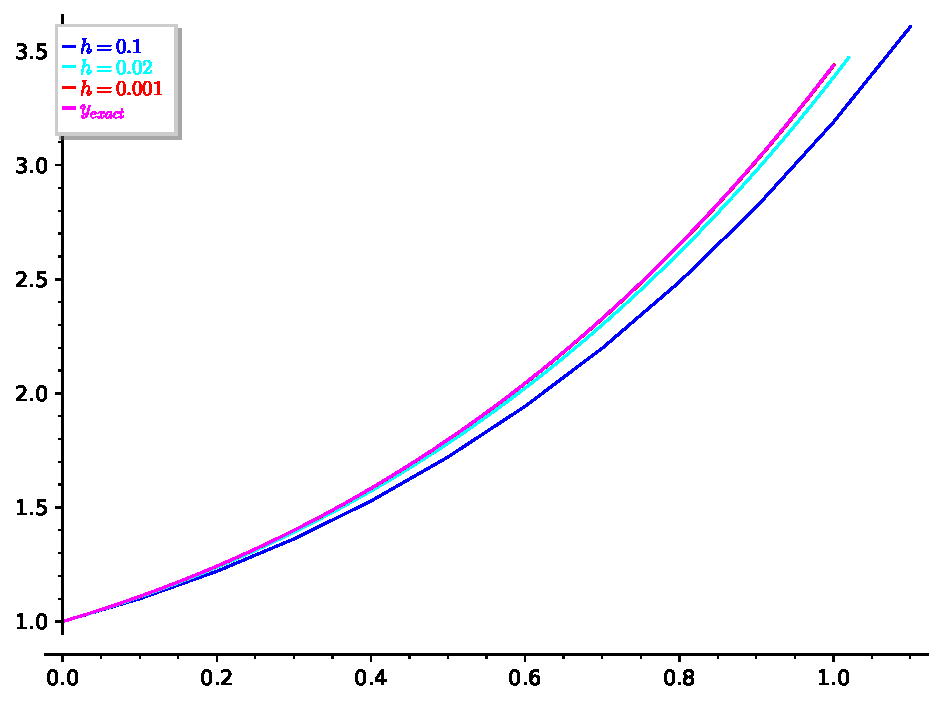
\includegraphics[width=\linewidth]{generated/sageplot/firstlook04-euler-approximation.pdf}%
\end{image}%
\tcblower
\end{figureptx}%
\begin{tableptx}{\textbf{Step sizes for Euler's approximation}}{x:table:firstlook04-table-euler-approximation-step-size}{}%
\centering%
{\tabularfont%
\begin{tabular}{ccccc}\hrulemedium
\(t_k\)&\(h = 0.1\)&\(h = 0.02\)&\(h = 0.001\)&Exact Solution\tabularnewline\hrulemedium
0.1&1.1000&1.1082&1.1102&1.1103\tabularnewline[0pt]
0.2&1.2200&1.2380&1.2426&1.2428\tabularnewline[0pt]
0.3&1.3620&1.3917&1.3993&1.3997\tabularnewline[0pt]
0.4&1.5282&1.5719&1.5831&1.5836\tabularnewline[0pt]
0.5&1.7210&1.7812&1.7966&1.7974\tabularnewline[0pt]
0.6&1.9431&2.0227&2.0431&2.0442\tabularnewline[0pt]
0.7&2.1974&2.2998&2.3261&2.3275\tabularnewline[0pt]
0.8&2.4872&2.6161&2.6493&2.6511\tabularnewline[0pt]
0.9&2.8159&2.9757&3.0170&3.1092\tabularnewline[0pt]
1.0&3.1875&3.3832&3.4238&3.4366\tabularnewline\hrulemedium
\end{tabular}
}%
\end{tableptx}%
\begin{activity}{Euler's Method and Error.}{g:activity:idp105545991511184}%
Consider the initial value problem%
\begin{align*}
y' \amp  = x + xy\\
y(0) \amp = 1.
\end{align*}
%
\begin{enumerate}[font=\bfseries,label=(\alph*),ref=\alph*]
\item{}Use separation of variables to solve the initial value problem.%
\item\label{x:task:firstlook04-task-exact}Compute \(y(x)\) for \(x = 0, 0.2, 0.4, \ldots, 1\).%
\item\label{x:task:firstlook04-task-euler}Use Euler's method to approximate solutions to the initial value problem for \(x = 0, 0.2, 0.4, \ldots, 1\).%
\item{}Compare the exact values of the solution (\hyperref[x:task:firstlook04-task-exact]{Task~{\xreffont\ref{g:activity:idp105545991511184}}.{\xreffont\ref{x:task:firstlook04-task-exact}}}) to the approximate values of the solution (\hyperref[x:task:firstlook04-task-euler]{Task~{\xreffont\ref{g:activity:idp105545991511184}}.{\xreffont\ref{x:task:firstlook04-task-euler}}}) and comment on what happens as \(x\) varies from \(0\) to \(1\).%
\end{enumerate}
\end{activity}%
\end{subsectionptx}
%
%
\typeout{************************************************}
\typeout{Subsection 1.4.2 Finding an Error Bound}
\typeout{************************************************}
%
\begin{subsectionptx}{Finding an Error Bound}{}{Finding an Error Bound}{}{}{x:subsection:firstlook04-subsection-error-bound}
To fully understand Euler's method, we will need to recall Taylor's theorem from calculus.%
\begin{theorem}{}{}{x:theorem:firstlook04-theorem-taylor}%
If \(x \gt x_0\), then%
\begin{equation*}
f(x) = f(x_0) + f'(x_0)(x - x_0) + \frac{f''(x_0)}{2!} (x - x_0)^2 + \cdots + \frac{f^{(n)}(\xi)}{n!}(x - x_0)^n,
\end{equation*}
where \(\xi \in (x_0, x)\).\index{Taylor's theorem}%
\end{theorem}
Given the initial value problem%
\begin{align*}
y' & = f(t, y),\\
y_0 & = y (t_0),
\end{align*}
choose \(t_1, t_2, \ldots, t_N\) to be equally spaced on \([t_0, a]\), we can write%
\begin{equation*}
t_k = t_0 + kh,
\end{equation*}
where \(h = (a - t_0)/N\) and \(k = 1, 2, \ldots, N\). Taylor's Theorem tells us that%
\begin{equation*}
y(t_{k + 1}) = y(t_k + h) = y(t_k) + y'(t_k) h + \frac{y''(t_k)}{2!} h^2 + \cdots.
\end{equation*}
If we know the values of \(y\) and its derivatives at \(t_k\), then we can determine the value of \(y\) at \(t_{k + 1}\).%
\par
The simplest approximation can be obtained by taking the first two terms of the Taylor series. That is, we will use a linear approximation,%
\begin{equation*}
y_{k + 1} = y(t_{k+1}) \approx y(t_k) + y'(t_k) h = y(t_k) + f(t_k, y_k) h.
\end{equation*}
This gives us Euler's method,%
\begin{align*}
Y_0 & = y(t_0)\\
Y_1 & = Y_0 + h f(t_0, Y_0)\\
Y_2 & = Y_1 + h f(t_1, Y_1)\\
& \vdots\\
Y_{k+1} & = Y_k + h f(t_k, Y_k).
\end{align*}
The terms that we are omitting, all contain powers of \(h\) of at least degree two. If \(h\) is small, then \(h^n\) for \(n = 2, 3, \ldots\) will be very small and these terms will not matter much.%
\par
We can actually estimate the error incurred by Euler's method if we make use of Taylor's Theorem.%
\begin{theorem}{}{}{x:theorem:firstlook04-theorem-euler-error-bound}%
Let \(y\) be the unique solution to the initial value problem\index{Euler's method!error bound}%
\begin{align*}
y' & =  f(t, y),\\
y(a) & =  \alpha,
\end{align*}
where \(t \in [a, b]\). Suppose that \(f\) is continuous and  there exists a constant \(L \gt 0\) such that%
\begin{equation*}
|f(t, y_1) - f(t, y_2)| \leq L |y_1 - y_2|,
\end{equation*}
whenever \((t, y_1)\) and \((t, y_2)\) are in \(D = [a, b] \times {\mathbb R}\). Also assume that there exists an \(M\) such that%
\begin{equation*}
|y''(t)| \leq M
\end{equation*}
for all \(t \in [a, b]\). If \(Y_0, \ldots, Y_N\) are the approximations generated by Euler's method for some positive integer \(N\), then%
\begin{equation*}
|y(t_i) - Y_i| \leq \frac{hM}{2L} [ e^{L(t_i - a)} - 1].
\end{equation*}
%
\end{theorem}
The condition that  there exists a constant \(L \gt 0\) such that%
\begin{equation*}
|f(t, y_1) - f(t, y_2)| \leq L |y_1 - y_2|,
\end{equation*}
whenever \((t, y_1)\) and \((t, y_2)\) are in \(D = [a, b] \times {\mathbb R}\) is called a \terminology{Lipschitz condition}\index{Lipschitz condition}. Many of the functions that we will consider satisfy such a condition. If the condition is satisfied, we can usually say a great deal about the function.%
\begin{tableptx}{\textbf{Error bound and actual error}}{x:table:firstlook04-table-euler-approximation-error-bound}{}%
\centering%
{\tabularfont%
\begin{tabular}{cccccc}\hrulemedium
\(k\)&\(t_k\)&\(Y_k\)&\(y_k = y(t_k)\)&\(|y_k - Y_k|\)&Estimated Error\tabularnewline\hrulemedium
0&0.0&1.0000&1.0000&0.0000&0.0000\tabularnewline[0pt]
1&0.1&1.1000&1.1103&0.0103&0.0286\tabularnewline[0pt]
2&0.2&1.2200&1.2428&0.0228&0.0602\tabularnewline[0pt]
3&0.3&1.3620&1.3997&0.0377&0.0951\tabularnewline[0pt]
4&0.4&1.5282&1.5836&0.0554&0.1337\tabularnewline[0pt]
5&0.5&1.7210&1.7974&0.0764&0.1763\tabularnewline[0pt]
6&0.6&1.9431&2.0442&0.1011&0.2235\tabularnewline[0pt]
7&0.7&2.1974&2.3275&0.1301&0.2756\tabularnewline[0pt]
8&0.8&2.4872&2.6511&0.1639&0.3331\tabularnewline[0pt]
9&0.9&2.8159&3.1092&0.2033&0.3968\tabularnewline[0pt]
10&1.0&3.1875&3.4366&0.2491&0.4671\tabularnewline\hrulemedium
\end{tabular}
}%
\end{tableptx}%
We can now compare the estimated error from our theorem to the actual error of our example. We first need to determine \(M\) and \(L\). Since%
\begin{equation*}
|f(t, y_1) - f(t, y_2)| = |(y_1 + t) - (y_2 + t)| = |y_1 - y_2|,
\end{equation*}
we can take \(L\) to be one.  Since \(y'' = 2e^t\), we can bound \(y''\) on the interval \([0, 1]\) by \(M = 2e\). Thus, we can bound the error by%
\begin{equation*}
|y(t_i) - Y_i| \leq \frac{hM}{2L} [ e^{L(t_i - a)} - 1] = 0.1e( e^{t_i } - 1)
\end{equation*}
for \(h =0.1\). Our results are in \hyperref[x:table:firstlook04-table-euler-approximation-error-bound]{Table~{\xreffont\ref{x:table:firstlook04-table-euler-approximation-error-bound}}}.%
\end{subsectionptx}
%
%
\typeout{************************************************}
\typeout{Subsection 1.4.3 Improving Euler's Method}
\typeout{************************************************}
%
\begin{subsectionptx}{Improving Euler's Method}{}{Improving Euler's Method}{}{}{x:subsection:firstlook04-subsection-improving-euler}
If we wish to improve upon Euler's method, we could add more terms of Taylor series. For example, we can obtain a more accurate approximation by using a quadratic Taylor polynomial,\index{Euler's method!improved}%
\begin{equation*}
y(t_1) \approx y_0 + f(t_0, y_0) h + \frac{y''(t_0)}{2} h^2.
\end{equation*}
However, we need to know \(y''(t_0)\) in order to use this approximation. Using the chain rule from multivariable calculus, we can differentiate both sides of \(y' = f(t, y)\) to obtain%
\begin{equation*}
y'' = \frac{\partial f}{\partial t} \frac{dt}{dt} + \frac{\partial f}{\partial y} \frac{dy}{dt} = f_t + f f_y.
\end{equation*}
Thus, our approximation becomes%
\begin{equation*}
y(t_1) \approx y_0 + f(t_0, y_0) h + \frac{1}{2} \left( f_t(t_0, y_0) + f(t_0, y_0) f_y (t_0, y_0) \right) h^2.
\end{equation*}
%
\par
The problem is that some preliminary analytic work must be done. That is, before we can write a program to compute our solution, we must find \(\partial f/\partial t\) and \(\partial f / \partial y\), although this is less of a problem with the availability of computer algebra systems such as \emph{Sage}.%
\par
Around 1900, two German mathematicians, Carle Runge and Martin Kutta, independently invented several numerical algorithms to solve differential equations. These methods, known as \terminology{Runge-Kutta methods}\index{Runge-Kutta method}, estimate the higher-order terms of the Taylor series to find an approximation that does not depend on computing derivatives of \(f(t, y)\).%
\par
If we consider the initial value problem%
\begin{align*}
y' & = f(t, y),\\
y(t_0) & = y_0,
\end{align*}
then%
\begin{equation*}
y(t_1) = y(t_0) + \int_{t_0}^{t_1} f(s, y(s)) \, ds
\end{equation*}
or%
\begin{equation}
y_1 - y_0 = y(t_1) - y(t_0) = \int_{t_0}^{t_1} f(s, y(s)) \, ds\label{x:men:firstlook04-equation-runge-kutta-1}
\end{equation}
by the Fundamental Theorem of Calculus. In Euler's method, we approximate the right-hand side of \hyperref[x:men:firstlook04-equation-runge-kutta-1]{({\xreffont\ref{x:men:firstlook04-equation-runge-kutta-1}})} by%
\begin{equation*}
y_1 - y_0 = f(t_0, y_0) h.
\end{equation*}
In terms of the definite integral, this is simply a left-hand sum. In the \terminology{improved Euler's method}\index{Euler's method!improved} or the \terminology{second-order Runge-Kutta method}\index{Runge-Kutta method!second-order} we will estimate the right-hand side of \hyperref[x:men:firstlook04-equation-runge-kutta-1]{({\xreffont\ref{x:men:firstlook04-equation-runge-kutta-1}})} using the trapezoid rule from calculus,%
\begin{align*}
y(t_1) - y(t_0) & = \int_{t_0}^{t_1} f(s, y(s)) \, ds\\
& \approx \left( f(t_0, y_0) + f(t_1, y_1) \right) \frac{h}{2}.
\end{align*}
Thus, our algorithm becomes%
\begin{equation}
y_1 = y_0 + \left( f(t_0, y_0) + f(t_1, y_1) \right) \frac{h}{2}.\label{x:men:firstlook04-equation-runge-kutta-2}
\end{equation}
However, we have a problem since \(y_1\) appears in the right-hand side of our approximation. To get around this difficulty, we will replace \(y_1\) in the right-hand side of \hyperref[x:men:firstlook04-equation-runge-kutta-2]{({\xreffont\ref{x:men:firstlook04-equation-runge-kutta-2}})} with the Euler approximation for \(y_1\). Thus,%
\begin{equation*}
y_1 = y_0 + \left( f(t_0, y_0) + f(t_1, y_0 + f(t_0, y_0) h) \right) \frac{h}{2}.
\end{equation*}
%
\par
To understand that the second-order Runge-Kutta method is actually an improvement over the traditional Euler's method, we will need to use the Taylor approximation for a function of two variables. Let us assume that \(f(x,y)\) is defined on some rectangle and that all of the derivatives of \(f\) are continuously differentiable. Then%
\begin{align*}
f(x + h, y + k) & = f(x, y) + h \frac{\partial}{\partial x} f(x, y) + k \frac{\partial}{\partial y}f(x, y)\\
& + \frac{1}{2!} \left( h^2 \frac{\partial^2}{\partial^2 x} f(x, y) + hk \frac{\partial^2}{\partial x \partial y}f(x, y) + k^2 \frac{\partial^2}{\partial^2 y}f(x, y) \right)\\
& + \frac{1}{3!} \left( h^3 \frac{\partial^3}{\partial^3 x} f(x, y)  + 3h^2k \frac{\partial^3}{\partial^2 x \partial y}f(x, y) \right.\\
& + \left. hk^2 \frac{\partial^3}{\partial x\partial^2 y}f(x, y) + k^3 \frac{\partial^3}{\partial^3 y} f(x, y) \right) + \cdots.
\end{align*}
As in the case of the single variable Taylor series, we can write a Taylor polynomial if the Taylor series is truncated,%
\begin{align*}
f(x + h, y + k) & =  \sum_{n = 0}^{N} \frac{1}{n!} \left(  h \frac{\partial}{\partial x} + k \frac{\partial}{\partial y} \right)^n f(x, y)\\
& + \frac{1}{(N+1)!} \left(  h \frac{\partial}{\partial x} + k \frac{\partial}{\partial y} \right)^{N+1} f(\overline{x}, \overline{y} ),
\end{align*}
where the second term is the remainder term and \((\overline{x}, \overline{y} )\) lies on the line segment joining \((x, y)\) and \((x + h, y + k)\).%
\par
In the Improved Euler's Method, we adopt a formula%
\begin{equation*}
y(t + h) = y(t) + w_1 F_1 + w_2 F_2,
\end{equation*}
where%
\begin{align*}
F_1 & = h f(t, y)\\
F_2 & = h f(t + \alpha h, y + \beta F_1).
\end{align*}
That is,%
\begin{equation}
y(t + h) = y(t) + w_1 h f(t, y) + w_2 h f(t + \alpha h, y + \beta h f(t, y)).\label{x:men:firstlook04-equation-runge-kutta-3}
\end{equation}
The idea is to choose the constants \(w_1\), \(w_2\), \(\alpha\), and \(\beta\) as accurately as possible in order to duplicate as many terms as possible in the Taylor series%
\begin{equation}
y(t + h) = y(t) + h y'(t) + \frac{h^2}{2!} y''(t) + \frac{h^3}{3!} y''(t) + \cdots.\label{x:men:firstlook04-equation-runge-kutta-4}
\end{equation}
We can make equations \hyperref[x:men:firstlook04-equation-runge-kutta-3]{({\xreffont\ref{x:men:firstlook04-equation-runge-kutta-3}})} and \hyperref[x:men:firstlook04-equation-runge-kutta-4]{({\xreffont\ref{x:men:firstlook04-equation-runge-kutta-4}})} agree if we choose \(w_1 = 1\) and \(w_2 = 0\). Since \(y' = f\), we obtain Euler's method.%
\par
If we are more careful about choosing our parameters, we can obtain agreement up through the \(h^2\) term. If we use the two variable Taylor series to expand \(f(t + \alpha h, y + \beta h f)\), we have%
\begin{equation*}
f(t + \alpha h, y + \beta h f) = f + \alpha h f_t + \beta h f f_y + {\mathcal O}(h^2),
\end{equation*}
where \({\mathcal O}(h^2)\) means that of the subsequent terms have a factor of \(h^n\) with \(n \geq 2\). Using this expression, we obtain a new form for \hyperref[x:men:firstlook04-equation-runge-kutta-3]{({\xreffont\ref{x:men:firstlook04-equation-runge-kutta-3}})},%
\begin{equation}
y(t + h) = y(t) + (w_1 + w_2) hf + \alpha w_2 h^2 f_t + \beta w_2 h^2 f f_y + {\mathcal O}(h^3).\label{x:men:firstlook04-equation-runge-kutta-5}
\end{equation}
Since \(y'' = f_t + f_y f\) by the chain rule, we can rewrite \hyperref[x:men:firstlook04-equation-runge-kutta-4]{({\xreffont\ref{x:men:firstlook04-equation-runge-kutta-4}})} as%
\begin{equation}
y(t + h) = y(t) + h f + \frac{h^2}{2!}( f_t +  f f_y) + {\mathcal O}(h^3).\label{x:men:firstlook04-equation-runge-kutta-6}
\end{equation}
We can make equations \hyperref[x:men:firstlook04-equation-runge-kutta-5]{({\xreffont\ref{x:men:firstlook04-equation-runge-kutta-5}})} and \hyperref[x:men:firstlook04-equation-runge-kutta-6]{({\xreffont\ref{x:men:firstlook04-equation-runge-kutta-6}})} agree up through the quadratic terms if we require that%
\begin{align*}
w_1 + w_2 & = 1,\\
\alpha w_2 & = \frac{1}{2},\\
\beta w_2 & = \frac{1}{2}.
\end{align*}
If we choose \(\alpha = \beta = 1\) and \(w_1 = w_2 = 1/2\), these equations are satisfied, and we obtain the improved Euler's method%
\begin{equation*}
y(t + h) = y(t) + \frac{h}{2} f(t, h) + \frac{h}{2} f(t + h, y  + h f(t, y)).
\end{equation*}
%
\par
The improved Euler's method or the second-order Runge-Kutta method is a more sophisticated algorithm that is less prone to error due to the step size \(h\). Euler's method is based on truncating the Taylor series after the linear term. Since%
\begin{equation*}
y(t + h) = y(t) + h y'(t) + {\mathcal O}(h^2),
\end{equation*}
we know that the error depends on \(h\). On the other hand, the error for the improved Euler's method depends on \(h^2\), since%
\begin{equation*}
y(t + h) = y(t) + h y'(t) + \frac{h^2}{2!} y''(t) + {\mathcal O}(h^3).
\end{equation*}
%
\par
If we use Simpson's rule to estimate the integral in%
\begin{equation*}
y(t_1) - y(t_0) = \int_{t_0}^{t_1} f(s, y(s)) \, ds,
\end{equation*}
we can improve our accuracy up to \(h^4\).  The idea is exactly the same, but the algebra becomes much more tedious. This method is known as the Runge-Kutta method of order 4 and is given by\index{Runge-Kutta method!order 4}%
\begin{equation*}
y(t + h) = y(t) + \frac{1}{6} (F_1 + 2 F_2 + 2 F_3 + F_4),
\end{equation*}
where%
\begin{align*}
F_1 & = h f(t, y)\\
F_2 & = hf\left( t + \frac{1}{2} h, y + \frac{1}{2} F_1 \right)\\
F_3 & = hf\left(  t + \frac{1}{2} h, y + \frac{1}{2} F_2 \right)\\
F_4 & = hf(t + h, y + F_3).
\end{align*}
%
\end{subsectionptx}
%
%
\typeout{************************************************}
\typeout{Subsection 1.4.4 Important Lessons}
\typeout{************************************************}
%
\begin{subsectionptx}{Important Lessons}{}{Important Lessons}{}{}{x:subsection:firstlook04-subsection-important-lessons}
%
\begin{itemize}[label=\textbullet]
\item{}We can use Euler's method to find an approximate solution to the initial value problem%
\begin{align*}
y' & = f(t, y),\\
y(a) & = \alpha
\end{align*}
on an interval \([a, b]\).  If we wish to find approximations at \(N\) equally spaced points \(t_1, \ldots, t_N\), where \(h = (b-a)/N\) and \(t_i = a + i h\), our approximations should be%
\begin{align*}
Y_0 & = \alpha,\\
Y_1 & = Y_0 + h f(\alpha, Y_0),\\
Y_2 & = Y_1 + h f(t_1, Y_1,)\\
& \vdots\\
Y_{k+1} & = Y_k + h f(t_k, Y_k),\\
Y_N & = Y_{N-1} + h f(t_{N-1}, Y_{N-1}).
\end{align*}
In practice, no one uses Euler's method. The Runge-Kutta methods are better algorithms.%
\item{}Taylor's Theorem is a very useful tool for studying differential equations. If \(x \gt x_0\), then%
\begin{equation*}
f(x) = f(x_0) + f'(x_0)(x - x_0) + \frac{f''(x_0)}{2!} (x - x_0)^2 + \cdots + \frac{f^{(n)}(\xi)}{n!}(x - x_0)^n,
\end{equation*}
where \(\xi \in (x_0, x)\).%
\item{}Error analysis rate of convergence is very important for any numerical algorithm. Our approximation is more accurate for smaller values of \(h\). Under reasonable conditions we can also bound the error by%
\begin{equation*}
|y(t_i) - Y_i| \leq \frac{hM}{2L} [ e^{L(t_i - a)} - 1],
\end{equation*}
where \(y\) is the unique solution to the initial value problem%
\begin{align*}
y' & = f(t, y),\\
y(a) & = \alpha.
\end{align*}
%
\item{}The condition that there exists a constant \(L \gt 0\) such that%
\begin{equation*}
|f(t, y_1) - f(t, y_2)| \leq L |y_1 - y_2|,
\end{equation*}
whenever \((t, y_1)\) and \((t, y_2)\) are in \(D = [a, b] \times {\mathbb R}\) is called a \terminology{Lipschitz condition}.%
\item{}Using Taylor series, we can develop better numerical algorithms to compute solutions of differential equations. The Runge-Kutta methods are an important class of these algorithms.%
\item{}The improved Euler's method is given by%
\begin{equation*}
y(t + h) = y(t) + \frac{h}{2} f(t, h) + \frac{h}{2} f(t + h, y + h f(t, y))
\end{equation*}
with the error bound depending on \(h^2\).%
\item{}The Runge-Kutta method of order 4 is given by%
\begin{equation*}
y(t + h) = y(t) + \frac{1}{6} (F_1 + 2 F_2 + 2 F_3 + F_4),
\end{equation*}
where%
\begin{align*}
F_1 & = h f(t, y)\\
F_2 & = hf\left( t + \frac{1}{2} h, y + \frac{1}{2} F_1 \right)\\
F_3 & = hf\left(  t + \frac{1}{2} h, y + \frac{1}{2} F_2 \right)\\
F_4 & = hf(t + h, y + F_3)
\end{align*}
with the error bound depending on \(h^4\).%
\end{itemize}
%
\end{subsectionptx}
%
%
\typeout{************************************************}
\typeout{Reading Questions 1.4.5 Reading Questions}
\typeout{************************************************}
%
\begin{reading-questions-subsection}{Reading Questions}{}{Reading Questions}{}{}{x:reading-questions:reading-questions-firstlook04}
\begin{divisionexercise}{1}{}{}{x:exercise:reading-questions-firstlook04-1}%
We can use Taylor polynomials to approximate a function \(f(x)\) near a point \(x_0\). Explain why this approximation can only be expected to be accurate near \(x_0\).%
\end{divisionexercise}%
\begin{divisionexercise}{2}{}{}{x:exercise:reading-questions-firstlook04-2}%
Should we always use Euler's method when approximating a solution to an initial value problem?  Why or why not?%
\end{divisionexercise}%
\end{reading-questions-subsection}
%
%
\typeout{************************************************}
\typeout{Exercises 1.4.6 Exercises}
\typeout{************************************************}
%
\begin{exercises-subsection}{Exercises}{}{Exercises}{}{}{x:exercises:exercises-firstlook04}
\par\medskip\noindent%
\textbf{Finding Solutions.}\space\space\hypertarget{x:exercisegroup:firstlook04-exercises-euler}{}%
For each of the initial value problem%
\begin{align*}
y' & = f(t, y),\\
y(t_0) & = y_0
\end{align*}
in \hyperlink{x:exercisegroup:firstlook04-exercises-euler}{Exercise Group~{\xreffont 1.4.6.1\textendash{}6}},%
\begin{enumerate}[label=(\alph*)]
\item{}Write the Euler's method iteration \(Y_{k+1} = Y_k + h f(t_k, Y_k)\) for the given problem, identifying the values \(t_0\) and \(y_0\).%
\item{}Using a step size of \(h = 0.1\), compute the approximations for \(Y_1\), \(Y_2\), and \(Y_3\).%
\item{}Solve the problem analytically if possible. If it is not possible for you to find the analytic solution, use \emph{Sage}.%
\item{}Use the results of (c) and (d), to construct a table of errors for \(Y_i - y_i\) for \(i = 1, 2, 3\).%
\end{enumerate}
%
\begin{exercisegroupcol}{2}
\begin{divisionexerciseegcol}{1}{}{}{g:exercise:idp105545991337616}%
\(y' = -2y\), \(y(0) = 0\)%
\end{divisionexerciseegcol}%
\begin{divisionexerciseegcol}{2}{}{}{g:exercise:idp105545991338640}%
\(y' = ty\), \(y(0) = 1\)%
\end{divisionexerciseegcol}%
\begin{divisionexerciseegcol}{3}{}{}{g:exercise:idp105545991339664}%
\(y' = y^3\), \(y(0) = 1\)%
\end{divisionexerciseegcol}%
\begin{divisionexerciseegcol}{4}{}{}{g:exercise:idp105545991340688}%
\(y' = y\), \(y'(0) = 1\)%
\end{divisionexerciseegcol}%
\begin{divisionexerciseegcol}{5}{}{}{g:exercise:idp105545991341712}%
\(y' = y + t\), \(y'(0) = 2\)%
\par\smallskip%
\noindent\textbf{\blocktitlefont Hint}.\hypertarget{g:hint:idp105545991342736}{}\quad{}This equation is a first-order linear equation (\hyperref[x:section:firstlook05]{Section~{\xreffont\ref{x:section:firstlook05}}}), but it is possible to find the analytic solution using \emph{Sage} (\hyperref[x:subsection:firstlook02-subsection-sage]{Subsection~{\xreffont\ref{x:subsection:firstlook02-subsection-sage}}}).%
\end{divisionexerciseegcol}%
\begin{divisionexerciseegcol}{6}{}{}{g:exercise:idp105545991377040}%
\(y' = 1/y\), \(y'(0) = 2\)%
\end{divisionexerciseegcol}%
\end{exercisegroupcol}
\par\medskip\noindent
\begin{divisionexercise}{7}{}{}{g:exercise:idp105545991378064}%
Consider the differential equation%
\begin{equation*}
\frac{dy}{dt} = 3y - 1
\end{equation*}
with initial value \(y(0) = 2\).%
\begin{enumerate}[label=(\alph*)]
\item{}Find the exact solution of the initial value problem.%
\item{}Use Euler's method with step size \(h = 0.5\) to approximate the solution to the initial value problem on the interval \([0,2]\)  Your solution should include a table of approximate values of the dependent variable as well as the exact values of the dependent variable.  Make sure that your approximations are accurate to \emph{four} decimal places.%
\item{}Sketch the graph of the approximate and exact solutions.%
\item{}Use the error bound theorem (\hyperref[x:theorem:firstlook04-theorem-euler-error-bound]{Theorem~{\xreffont\ref{x:theorem:firstlook04-theorem-euler-error-bound}}}) to estimate the error at each approximation.  Your solution should include a table of approximate values of the dependent variable the exact values of the dependent variable, the error estimates, and the actual error.  Make sure that your approximations are accurate to \emph{four} decimal places.%
\end{enumerate}
%
\end{divisionexercise}%
\begin{divisionexercise}{8}{}{}{g:exercise:idp105545991382928}%
In this series of exercises, we will prove the error bound theorem for Euler's method (\hyperref[x:theorem:firstlook04-theorem-euler-error-bound]{Theorem~{\xreffont\ref{x:theorem:firstlook04-theorem-euler-error-bound}}}).%
\begin{enumerate}[label=(\alph*)]
\item{}Use Taylor's Theorem to show that for all \(x \geq -1\) and any positive \(m\),%
\begin{equation*}
0 \leq (1 + x)^m \leq e^{mx}.
\end{equation*}
%
\item{}Use part (1) and geometric series to prove the following statement: If \(s\) and \(t\) are positive real numbers, and \(\{ a_i \}_{i = 0}^k\) is a sequence satisfying%
\begin{align*}
a_0 & \geq -\frac{t}{s}\\
a_{i+1} & \leq (1 + s) a_i + t, \text{ for }i = 0, 1, 2, \ldots, k,
\end{align*}
then%
\begin{equation*}
a_{i + 1} \leq e^{(i + 1)s} \left(  \frac{t}{s} + a_0 \right) - \frac{t}{s}.
\end{equation*}
%
\item{}When \(i = 0\), \(y(t_0) = Y_0 = \alpha\) and the theorem is true.  Use Euler's method and Taylor's Theorem to show that%
\begin{equation*}
|y_{i + 1} - Y_{i + 1} | \leq |y_i - Y_i| + h |f(t_i, y_i) - f(t_i, Y_i)| + \frac{h^2}{2} |y''(\xi_i)|
\end{equation*}
where \(\xi_i \in (t_i, t_{i+1})\) and \(y_k = y(t_k)\).%
\item{}Show that%
\begin{equation*}
|y_{i + 1} - Y_{i + 1} | \leq  |y_i - Y_i| (1 + hL) + \frac{Mh^2}{2}. 
\end{equation*}
%
\item{}Let \(a_j = |y_j - Y_j|\) for \(j = 0, 1, \ldots, N\), \(s = hL\), and \(t = M h^2/2\) and apply part (2) to show%
\begin{equation*}
|y_{i + 1} - Y_{i + 1} | \leq e^{(1 + i)hL} \left( |y_0 - Y_0| + \frac{M h^2 }{2hL} \right) - \frac{M h^2}{2hL}. 
\end{equation*}
and derive that%
\begin{equation*}
|y_{i + 1} - Y_{i + 1} | \leq \frac{M h }{2L} \left( e^{(t_{i+ 1} - a)L} - 1\right)
\end{equation*}
for each \(i = 0, 1, \ldots, N-1\).%
\end{enumerate}
%
\par\smallskip%
\noindent\textbf{\blocktitlefont Hint}.\hypertarget{g:hint:idp105545991361296}{}\quad{}Hints for part (2):%
\begin{itemize}[label=\textbullet]
\item{}For fixed \(i\) show that%
\begin{align*}
a_{i + 1} & \leq (1 + s)a_i + t\\
& \leq (1 + s)[(1 + s)a_{i - 1}+ t] + t\\
& \leq (1 + s)\{ (1 + s)[(1 + s) a_{i - 2} + t]+ t\} + t\\
& \vdots\\
& \leq (1 + s)^{i+1}a_0 + [1 + (1 + s) + (1+s)^2 + \cdots + (1 + s)^i]t.
\end{align*}
%
\item{}Now use a geometric sum to show that%
\begin{equation*}
a_{i + 1} \leq (1 + s)^{i + 1} a_0 + \frac{t}{s}[(1 + s)^{i + 1} - 1] = (1 + s)^{i + 1} \left( \frac{t}{s} + a_0 \right) - \frac{t}{s}.
\end{equation*}
%
\item{}Apply part (1) to derive%
\begin{equation*}
a_{i + 1} \leq e^{(i + 1)s} \left( \frac{t}{s} + a_0 \right) - \frac{t}{s}.
\end{equation*}
%
\end{itemize}
%
\end{divisionexercise}%
\end{exercises-subsection}
%
%
\typeout{************************************************}
\typeout{Subsection 1.4.7 Sage\textemdash{}Numerical Routines for solving ODEs}
\typeout{************************************************}
%
\begin{subsectionptx}{Sage\textemdash{}Numerical Routines for solving ODEs}{}{Sage\textemdash{}Numerical Routines for solving ODEs}{}{}{x:subsection:firstlook04-subsection-sage-project}
Not all differential equations can be solved using algebra and calculus even if we are very clever. If we encounter an equation that we cannot solve or use \emph{Sage} to solve, we must resort to numerical algorithms like Euler's method or one of the Runge-Kutta methods, which are best implemented using a computer. Fortunately, \emph{Sage} has some very good numerical solvers. \emph{Sage} will need to know the following to solve a differential equation:%
\begin{itemize}[label=\textbullet]
\item{}An abstract function,%
\item{}A differential equation, \emph{including an initial condition},%
\item{}A \emph{Sage} command to solve the equation.%
\end{itemize}
%
\par
Suppose we wish to solve the initial value problem \(dy/dx = x + y\), \(y(0) = 1\). We can use \emph{Sage} to find an algebraic solution.%
\begin{sageinput}
y = function('y')(x)
de = diff(y,x) == x + y
solution = desolve(de, y, ics = [0,1])
solution.show()
plot(solution, x, 0, 5)
\end{sageinput}
\begin{sageoutput}

\end{sageoutput}
We can also use Euler's method to find a solution for our initial value problem.%
\begin{sageinput}
x,y = PolynomialRing(RR, 2, "xy").gens() #declare x, y as generators of a polynomial ring
eulers_method(x + y, 0,1, 0.5, 5)
\end{sageinput}
\begin{sageoutput}

\end{sageoutput}
The syntax of \mono{eulers\_method} for the inital value problem%
\begin{align*}
y \amp = f(x,y)\\
f(x_0) \amp = y_0
\end{align*}
with step size \(h\) on the interval \([x_0, x_1]\) is \mono{eulers\_method(f, x0, y0, h, x1)} Notice that we obtained a table of values. However, we can use the \mono{line} command from \emph{Sage} to plot the values \((x, y)\).%
\begin{sageinput}
x,y = PolynomialRing(RR, 2, "xy").gens()
pts = eulers_method(x + y, 0, 1, 1/2, 4.5, algorithm="none")
p = list_plot(pts, color="red")
p += line(pts)
p
\end{sageinput}
\begin{sageoutput}

\end{sageoutput}
As we pointed out, \mono{eulers\_method} is not very sophisticated. We have to use a very small step size to get good accuracy, and the method can generate errors if we are not careful. Fortunately, \emph{Sage} has much better algorithms for solving initial value problems.  One such algorithm is \mono{desolve\_rk4}, which implements the fourth order Runge-Kutta method.%
\begin{sageinput}
x,y = var('x y')
desolve_rk4(x + y, y, ics=[0, 1], end_points = 5, step = 0.5)
\end{sageinput}
\begin{sageoutput}

\end{sageoutput}
Again, we just get a list of points.  However, \mono{desolve\_rk4} has some nice built-in graphing utilities.%
\begin{sageinput}
x,y = var('x y')
p = desolve_rk4(x + y, y, ics = [0,1], ivar = x, output = 'slope_field', end_points = [0, 5], thickness = 2, color = 'red')
p
\end{sageinput}
\begin{sageoutput}

\end{sageoutput}
Write the \emph{Sage} commands to compare the graphs obtained using \mono{eulers\_method} and \mono{desolve} with the exact solution.%
\begin{sageinput}

\end{sageinput}
\begin{sageoutput}

\end{sageoutput}
Not only is \mono{desolve\_rk4} more accurate, it is much easier to use. For more information, see \href{http://www.sagemath.org/doc/reference/calculus/sage/calculus/desolvers.html}{\nolinkurl{www.sagemath.org/doc/reference/calculus/sage/calculus/desolvers.html}}.%
\end{subsectionptx}
\end{sectionptx}
%
%
\typeout{************************************************}
\typeout{Section 1.5 First-Order Linear Equations}
\typeout{************************************************}
%
\begin{sectionptx}{First-Order Linear Equations}{}{First-Order Linear Equations}{}{}{x:section:firstlook05}
\begin{objectives}{Objectives}{g:objectives:idp105545991418384}
%
\begin{itemize}[label=\textbullet]
\item{}To understand that any \terminology{first-order linear differential equation}%
\begin{equation*}
y' + p(x) y = g(x)
\end{equation*}
can be solved by multiplying each side of the equation by an \terminology{integrating factor}.%
\item{}To understand the existence and uniqueness of solutions to first-order initial value problems.%
\end{itemize}
\end{objectives}
\begin{introduction}{}%
A \terminology{first-order differential equation}\index{differential equation!first-order linear} is an equation of the form%
\begin{equation}
\frac{dx}{dt} + p(t) x = q(t).\label{x:men:firstlook05-equation-first-order-linear-ode}
\end{equation}
This equation will not be separable if \(p(t)\) is not a constant. We shall have to find a new approach to solving such an equation. We could, of course, use a numerical algorithm to solve~\hyperref[x:men:firstlook05-equation-first-order-linear-ode]{({\xreffont\ref{x:men:firstlook05-equation-first-order-linear-ode}})}; however, we can always find an algebraic solution to a first-order linear differential equation. Moreover, the fact that we can obtain such a solution analytically will prove very useful when we investigate more complicated equations and systems of equations.%
\end{introduction}%
%
%
\typeout{************************************************}
\typeout{Subsection 1.5.1 Mine Tailings}
\typeout{************************************************}
%
\begin{subsectionptx}{Mine Tailings}{}{Mine Tailings}{}{}{x:subsection:firstlook05-subsection-mine-tailings}
In any mining operation, tailings are what is left after everything of value has been extracted. For example, in a hard rock mining operation, ore is often pulverized and then processed using chemicals to extract certain minerals of value. Soft rock mining operations such as coal mining or extracting oil from tar sands might use solvents or water to extract any commodity of value. The material that is left over after the minerals, coal, or oil is extracted can often present huge environmental challenges. There are different ways of processing mine tailings, but one way is to store them in a pond, especially if water is used in the mining operation. This method allows any particles that are suspended in the water to settle to the bottom of the pond. The water can then be treated and recycled.%
\par
Suppose that we have a gold mining operation and we are storing our tailings in a pond that has an initial volume of 20,000 cubic meters.  When we begin our operation, the tailings pond is filled with clean water. The pond has a stream flowing into it, and water is also pumped out of the pond.  Chemicals are used in processing gold ore. These chemicals such as sodium cyanide can be highly poisonous and dangerous to the environment, and the water must be treated before it is released into the watershed. Suppose that 1000 cubic meters per day flow into the pond from stream and 1000 cubic meters are pumped from the pond each day to be processed and recycled. Thus, the water level of the pond remains constant.%
\par
At time \(t = 0\), the water from stream becomes contaminated with chemicals from the mining operation, say at a rate of 5 kilograms of chemicals per 1000 cubic meters. We will assume that water in our tailings pond is well mixed so that the concentration of chemicals through out the pond is fairly uniform. In addition, any particulate matter pumped into the pond from the stream settles to the bottom of the pond at a rate of 50 cubic meters per day. Thus, the volume of our tailings pond is reduced by 50 cubic meters each day, and our tailings pond will become full after 400 days of operation. We shall assume that the particulate matter and the chemicals are included in the 1000 cubic meters that flow into the pond from the stream each day.%
\par
We wish to find a differential equation that will model the amount of chemicals in the tailings pond at any particular time. Let \(x(t)\) be the amount of chemicals in the pond at time \(t\). Then \(dx/dt\) is the difference between the rate at which the chemicals are entering the pond and the rate at which the chemicals leave the pond.%
\begin{equation*}
\frac{dx}{dt} = \text{rate in} - \text{rate out}.
\end{equation*}
Since water flows into the pond from the stream at a rate of 1000 cubic meters per day, the rate at which the chemicals enter the pond is 5 kilograms per day. On the other hand, the rate at which the chemicals leave the pond will depend on the amount of chemicals in the pond at time \(t\). The volume of the pond is decreasing due to sediment, and at time \(t\) it is \(V(t) = 20000 - 50t\). Thus, the concentration of chemicals in the pond at time \(t\) is \(x/(20000 - 50 t)\), and the rate at which the chemicals are flowing out of the pond to be recycled is%
\begin{equation*}
1000 \left(  \frac{x}{20000 - 50t} \right) = \frac{20x}{ 400 - t}.
\end{equation*}
Hence, the differential equation that models the amount of chemical in the tailings pond at time \(t\) is%
\begin{equation}
\frac{dx}{dt} = 5 - \frac{20x}{ 400 - t}.\label{x:men:firstlook05-equation-mine-tailings-1}
\end{equation}
Of course, we will have to cease mining operations once the pond is full, since there will only be water in the pond if \(V(t) = 20000 - 50t \geq 0\); that is, when \(0 \leq t \lt 400\).%
\par
Notice that equation~\hyperref[x:men:firstlook05-equation-mine-tailings-1]{({\xreffont\ref{x:men:firstlook05-equation-mine-tailings-1}})} is not autonomous. In fact, it is not even separable. We will have to use a different approach to find a solution. First, we will rewrite the equation in the form%
\begin{equation*}
\frac{dx}{dt}  + \frac{20}{ 400 - t} x = 5.
\end{equation*}
If we multiply both sides of this equation by \((400 - t)^{-20}\), we obtain%
\begin{equation}
(400 - t)^{-20}\frac{dx}{dt} + 20(400 - t)^{-21} x = 5(400 - t)^{-20}.\label{x:men:firstlook05-equation-mine-tailings-2}
\end{equation}
We now make the crucial observation that the product rule applies to the lefthand side of our equation,%
\begin{equation*}
(400 - t)^{-20}\frac{dx}{dt} + 20(400 - t)^{-21} x = \frac{d}{dt} \left( (400 - t)^{-20}x \right).
\end{equation*}
Thus, equation~\hyperref[x:men:firstlook05-equation-mine-tailings-2]{({\xreffont\ref{x:men:firstlook05-equation-mine-tailings-2}})} becomes%
\begin{equation*}
\frac{d}{dt} \left( (400 - t)^{-20}x \right) = 5(400 - t)^{-20}.
\end{equation*}
Integrating both sides of this equation, we have%
\begin{equation*}
(400 - t)^{-20}x = 5 \int (400 - t)^{-20} \, dt = \frac{5(400 - t)^{-19}}{19} + C,
\end{equation*}
where \(C\) is an arbitrary constant.  Solving for \(x\), we obtain%
\begin{equation*}
x(t) = \frac{5}{19} (400 - t) + C(400 - t)^{20}.
\end{equation*}
Since \(x(0) = 0\), we can quickly determine that \(C = - (5/19)400^{-19}\) and that the solution to our initial value problem is%
\begin{equation*}
x(t) = \frac{5}{19} (400 - t) \left[ 1 - \left( \frac{400 - t}{400}  \right)^{19} \right].
\end{equation*}
The graph of the solution to our differential equation (\hyperref[x:figure:firstlook05-figure-tailings-pond]{Figure~{\xreffont\ref{x:figure:firstlook05-figure-tailings-pond}}}) fits the situation. Initially, there are no chemicals in the pond, but \(x(t)\) quickly increases. However, the amount of chemicals decreases as the pond begins to fill with sediment. Eventually, there are no chemicals at \(t = 400\).%
\begin{figureptx}{Chemical waste in a tailings pond}{x:figure:firstlook05-figure-tailings-pond}{}%
\begin{image}{0.2}{0.6}{0.2}%
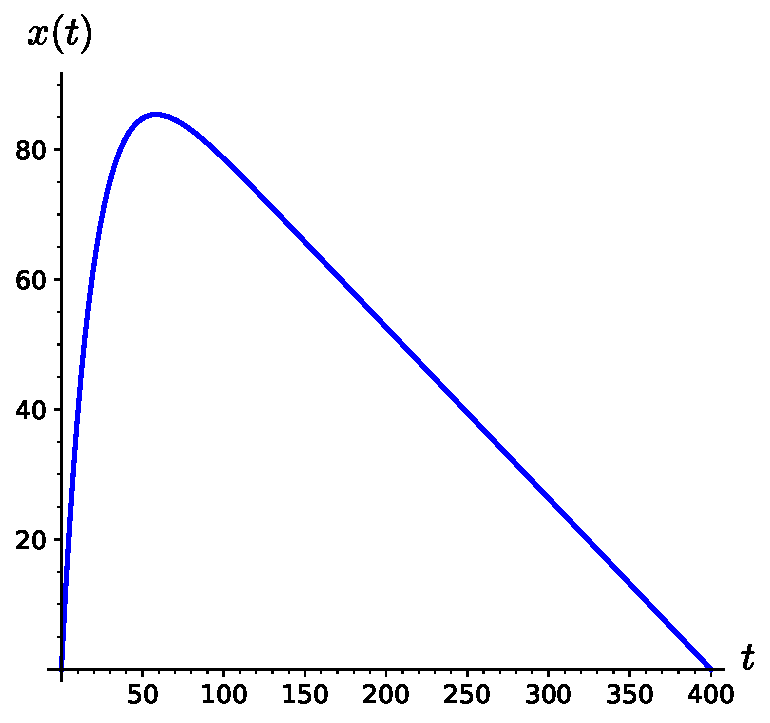
\includegraphics[width=\linewidth]{generated/sageplot/firstlook05-tailings-pond.pdf}%
\end{image}%
\tcblower
\end{figureptx}%
\end{subsectionptx}
%
%
\typeout{************************************************}
\typeout{Subsection 1.5.2 First-Order Linear Equations}
\typeout{************************************************}
%
\begin{subsectionptx}{First-Order Linear Equations}{}{First-Order Linear Equations}{}{}{x:subsection:firstlook05-subsection-first-order-linear-de}
The differential equation%
\begin{equation*}
\frac{dx}{dt} + \frac{20}{ 400 - t} x = 5
\end{equation*}
is an example of a first-order linear differential equation. More specifically, a \terminology{first-order linear differential equation}\index{differential equation!first-order linear} is an equation that can be written in the form%
\begin{equation*}
\frac{dx}{dt} + p(t) x = q(t).
\end{equation*}
Let us first show how to solve first-order linear equations when the coefficient functions are constant. If%
\begin{align*}
\frac{dx}{dt} + px & = q,\\
x(t_0) & = x_0,
\end{align*}
then we first multiply both sides of the equation by \(e^{pt}\) to obtain%
\begin{equation*}
e^{pt} \frac{dx}{dt} + e^{pt} px = q e^{pt}.
\end{equation*}
The left-hand side of the equation is \terminology{exact}\index{differential equation!exact}. That is,%
\begin{equation*}
e^{pt} \frac{dx}{dt} + e^{pt} px = \frac{d}{dt} \left(  x(t) e^{pt} \right).
\end{equation*}
If we integrate both sides of%
\begin{equation*}
\frac{d}{dt} \left(  x(t) e^{pt} \right)= q e^{pt},
\end{equation*}
then%
\begin{equation*}
x(t) e^{pt} = \frac{q}{p} e^{pt} + C.
\end{equation*}
If we apply the initial condition, we can determine \(C\),%
\begin{equation*}
C = \left( x_0 - \frac{q}{p} \right) e^{pt_0}.
\end{equation*}
Thus, the solution that we seek is%
\begin{equation*}
x(t) = \frac{q}{p} + \left( x_0 - \frac{q}{p} \right) e^{p(t_0 - t)}.
\end{equation*}
%
\begin{example}{}{g:example:idp105545993282576}%
Suppose we wish to solve the initial value problem%
\begin{align}
\frac{dx}{dt} -2 x & = 3,\label{x:mrow:firstlook05-equation-constant-coeff-1}\\
x(0) & = 1.\label{x:mrow:firstlook05-equation-constant-coeff-2}
\end{align}
Multiplying both sides of equation~\hyperref[x:mrow:firstlook05-equation-constant-coeff-1]{({\xreffont\ref{x:mrow:firstlook05-equation-constant-coeff-1}})} by \(e^{-2t}\), we obtain%
\begin{equation*}
\frac{d}{dt}\left( e^{-2t}x \right) = e^{-2t}\frac{dx}{dt} -2 e^{-2t}x = 3e^{-2t}.
\end{equation*}
Integrating both sides of this last equation, gives us the following%
\begin{equation*}
e^{-2t}x = 3 \int e^{-2t} \, dt + C = -\frac{3}{2} e^{-2t} + C.
\end{equation*}
Applying the initial condition \(x(0) = 1\), we can conclude that \(C = 5/2\), and%
\begin{equation*}
x(t) = \frac{5}{2} e^{2t} - \frac{3}{2}.
\end{equation*}
%
\end{example}
\begin{example}{}{x:example:firstlook05-example-nonconstant-coeff}%
Now let us solve a first-order linear differential equation where the coefficients are not constant. Suppose that%
\begin{equation*}
y' + 2xy = e^{-x^2},
\end{equation*}
where \(y(0) = 1\). We will multiply both sides of the equation by \(e^{x^2}\) and use the product rule to obtain%
\begin{equation*}
\frac{d}{dx} \left(  e^{x^2} y \right) = e^{x^2} y' + 2xe^{x^2}y =  e^{x^2} e^{-x^2} = 1.
\end{equation*}
Integrating both sides, we get%
\begin{equation*}
e^{x^2} y  = \int  dx +  C.
\end{equation*}
Thus, the general solution is%
\begin{equation*}
y = (x + C) e^{-x^2}.
\end{equation*}
Using the initial condition to solve for \(C\), we find that \(C = 1\) and%
\begin{equation*}
y = (x + 1)e^{-x^2}.  
\end{equation*}
We can use Sage to check our solution.%
\end{example}
\begin{sageinput}
x = var('x')
y = function('y')(x)
de = diff(y, x) + 2*x*y == exp(-x^2)
solution = desolve(de, y, ics = [0, 1])
solution.show()
\end{sageinput}
\begin{sageoutput}
(x + 1)*e^(-x^2)
\end{sageoutput}
Surprisingly, the strategy in \hyperref[x:example:firstlook05-example-nonconstant-coeff]{Example~{\xreffont\ref{x:example:firstlook05-example-nonconstant-coeff}}} will always work. Suppose that%
\begin{equation}
x' + p(t) x = q(t).\label{x:men:firstlook05-equation-first-order}
\end{equation}
If we choose \(P(t)\) such that \(P'(t) = p(t)\) and multiply both sides of the equation by \(e^{P(t)}\), then%
\begin{equation*}
\left( e^{P(t)} x \right)' = e^{P(t)} ( x'(t) + p(t) x(t) )= e^{P(t)} q(t).
\end{equation*}
Integrating both sides,%
\begin{equation*}
e^{P(t)} x = \int e^{P(t)} q(t) \, dt + C
\end{equation*}
or%
\begin{equation*}
x = \frac{1}{e^{P(t)} } \left( \int e^{P(t)} q(t) \, dt + C \right).
\end{equation*}
The Fundamental Theorem of Calculus tells us that \(P(t) = \int p(t) \, dt\). We say that%
\begin{equation*}
\mu(t) = e^{\int p(t) \, dt} = \exp\left(  \int p(t) \, dt \right)
\end{equation*}
is an \terminology{integrating factor}\index{integrating factor} for the differential equation~\hyperref[x:men:firstlook05-equation-first-order]{({\xreffont\ref{x:men:firstlook05-equation-first-order}})}.%
\begin{example}{}{g:example:idp105545993263888}%
Consider the initial value problem%
\begin{gather*}
\frac{dy}{dx} - \frac{2}{x} y = 2x^2\\
y(-2) = 4.
\end{gather*}
Our integrating factor is%
\begin{equation*}
\mu(x) = \exp\left( - \int \frac{2}{x} \, dx\right) = e^{-2 \ln x} = e^{\ln x^{-2}} = x^{-2}.
\end{equation*}
Multiplying both of our differential equation by \(\mu(x) = x^{-2}\), we obtain%
\begin{equation*}
x^{-2} \left(\frac{dy}{dx} - \frac{2}{x} y \right)  = 2
\end{equation*}
or%
\begin{equation*}
\frac{d}{dx}\left(  x^{-2} y \right) = x^{-2} \frac{dy}{dx} - 2 x^{-3} y  = 2.
\end{equation*}
We can now integrate this equation to get%
\begin{equation*}
x^{-2} y = 2x + C.
\end{equation*}
The initial condition \(y(-2) = 4\) allows us to find \(C = 5\). Therefore, the solution to our initial value problem is%
\begin{equation*}
y = 2x^3 + 5x^2.
\end{equation*}
%
\end{example}
\begin{activity}{Finding Solutions to First-Order Linear Differential Equations.}{g:activity:idp105545993267984}%
Solve each of the following initial value problems.%
\begin{enumerate}[font=\bfseries,label=(\alph*),ref=\alph*]
\item{}\(y' = 3y + t\); \(y(0) = 1\)%
\item{}\(x' = tx + 2t\); \(x(1) = 2\)%
\item{}\(y' = 2x - 3y + e^{-x}\); \(y(0) = 1\)%
\item{}\(\dfrac{du}{dt} = \dfrac{t - 1}{t} u + t^2\); \(u(1) = 0\)%
\item{}\(y' = \sin x - y\); \(y(0) = 1\)%
\end{enumerate}
\end{activity}%
\end{subsectionptx}
%
%
\typeout{************************************************}
\typeout{Subsection 1.5.3 Mixing Models}
\typeout{************************************************}
%
\begin{subsectionptx}{Mixing Models}{}{Mixing Models}{}{}{x:subsection:firstlook05-subsection-mixing-models}
Many applications involve the mixing of two or more substances together. As we mentioned previously, we can model how petroleum products are mixed together in a refinery, how various ingredients are mixed together in a brewery, or how greenhouse gases move across various layers of the earth's atmosphere.%
\begin{example}{}{g:example:idp105545993275024}%
Suppose that a 100-gallon tank initially contains 50 gallons of salt water containing five pounds of salt. A brine mixture containing one pound of salt per gallon flows into the top of the tank at a rate of 5 gallons per minute. A well mixed solution leaves the tank at rate of 4 gallons per minute. We wish to know how much salt is in the tank, when the tank is full.%
\par
To construct our model, we will let \(t\) be the time (measured in minutes) and set up a differential equation that will measure how fast the amount of salt at time \(t\), \(x(t)\), is changing. We have the initial condition \(x(0) = 5\), and%
\begin{align*}
\frac{dx}{dt} & = \text{rate of salt flowing in} - \text{rate of salt flowing out}\\
& = \underbrace{5}_{\text{in flow}} - \underbrace{4 \frac{x}{V(t)}}_{\text{out flow}},
\end{align*}
where \(V(t)\) is the volume at time \(t\). The expression \(x/V(t)\) is the amount of salt in one gallon at time \(t\). We have \(V(t) = 50 + t\), since the tank starts with 50 gallons and five gallons are pumped into the tank per minute while four gallons leave the tank during the same time interval. Thus, our differential equation becomes%
\begin{equation*}
\frac{dx}{dt} = 5 - \frac{4}{50 + t}x.
\end{equation*}
Our equation is linear since we can rewrite it as%
\begin{equation}
\frac{dx}{dt} + \frac{4}{50 + t} x = 5.\label{x:men:firstlook05-equation-mixing}
\end{equation}
%
\par
An integrating factor for this differential equation is%
\begin{equation*}
\mu(t) = \exp\left(  \int \frac{4}{50 + t} \, dt \right) = e^{4 \ln(50 + t)} = (50 + t)^4.
\end{equation*}
Therefore, if we multiply both sides of equation~\hyperref[x:men:firstlook05-equation-mixing]{({\xreffont\ref{x:men:firstlook05-equation-mixing}})} by \(\mu(t)\), we get%
\begin{equation*}
(50 + t)^4\frac{dx}{dt} + 4(t + 50)^3 x = 5(50 + t)^4.
\end{equation*}
We can now apply the product rule to obtain%
\begin{equation*}
\frac{d}{dt}[ (50 + t)^4 x] = 5(50 + t)^4.
\end{equation*}
Integrating both sides and simplifying gives us%
\begin{equation*}
x = t + 50 + \frac{C}{(t + 50)^4}.
\end{equation*}
Our initial condition, \(x(0) = 5\) tells us that \(C = -281{,}250{,}000\) and%
\begin{equation*}
x(t) = t + 50 - \frac{281250000}{(t + 50)^4}.
\end{equation*}
Thus, when the tank is full, \(t = 50\) and the amount of salt in the tank is \(x(50) = 97.188\) pounds. We can use \emph{Sage} to easily check the solution of our initial value problem.%
\end{example}
\begin{sageinput}
t = var('t')
x = function('x')(t)
de = diff(x, t) + 4*x/(50 + t) == 5
solution(t) = desolve(de, x, ics=[0, 5])
solution(50).n(digits = 5)
\end{sageinput}
\begin{sageoutput}
97.188
\end{sageoutput}
\begin{activity}{A Mixing Problem.}{g:activity:idp105545993319184}%
Suppose that a tank contains 1000 gallons of a solution consisting of 200 pounds of salt dissolved in water. Pure water is pumped into the tank at a rate of 6 gallons per minute. At the same time, the tank is drained at the same rate.  Assume that the brine mixture is kept well stirred.%
\begin{enumerate}[font=\bfseries,label=(\alph*),ref=\alph*]
\item{}Set up an initial value problem to model the amount of salt in the tank at time \(t\).%
\item{}How long will it take until there is only 20 pounds of salt left in the tank?.%
\end{enumerate}
\end{activity}%
\end{subsectionptx}
%
%
\typeout{************************************************}
\typeout{Subsection 1.5.4 Finance Models}
\typeout{************************************************}
%
\begin{subsectionptx}{Finance Models}{}{Finance Models}{}{}{x:subsection:firstlook05-subsection-finance-models}
There are a number of problems in finance that can be modeled using differential equations. Let \(P(t)\) be the balance of an account at time \(t\) and suppose that the account pays interest at a rate of \(r\) percent per year compounded continuously. Suppose that we also allow withdrawals of \(W\) dollars per year. The net increase in the balance between times \(t\) and \(t + \Delta t\) can now be described as%
\begin{equation*}
P(t + \Delta t) - P(t) \approx r P \Delta t - W \Delta t
\end{equation*}
Thus,%
\begin{equation*}
P'(t) = \lim_{\Delta t \rightarrow 0} \frac{P(t + \Delta t) - P(t) }{\Delta t} = rP - W.
\end{equation*}
%
\par
We can solve the equation%
\begin{equation*}
P' = rP - W
\end{equation*}
by multiplying both sides of the equation by the integrating factor%
\begin{equation*}
\mu(t) = \exp\left(- \int r \, dt\right) = e^{-rt}.
\end{equation*}
to obtain%
\begin{equation*}
\frac{d}{dt} [e^{-rt} P] = -We^{-rt}.
\end{equation*}
Integrating both sides of this equation, we have%
\begin{equation*}
e^{-rt} P = \frac{W}{r} e^{-rt} + C
\end{equation*}
or%
\begin{equation*}
P = \frac{W}{r} + Ce^{rt}.
\end{equation*}
If we know the initial balance in the account, say \(P(0) = P_0\), we can determine \(C\). That is,%
\begin{equation*}
P_0 = \frac{W}{r} + C
\end{equation*}
or%
\begin{equation*}
C = P_0 - \frac{W}{r}.
\end{equation*}
Thus, the solution to our initial value problem is%
\begin{equation*}
P = \frac{W}{r} + \left( P_0 - \frac{W}{r} \right) e^{rt}.
\end{equation*}
%
\begin{example}{}{g:example:idp105545993296656}%
Suppose that your parents have established a money market account with a balance of \textdollar{}50,000 that they will use to help you pay for your college education.  The account receives an average annual interest of 4\%. You estimate that your tuition, room and board, and other college expenses to be \textdollar{}20,000 per year.%
\par
We model this financial situation with the differential equation%
\begin{align*}
\frac{dP}{dt} \amp = 0.04P - 20000\\
P(0) \amp = 50000.
\end{align*}
Rewriting the differential equation as \(dP/dt - 0.04P = -20000\), our integrating factor becomes \(\mu(t) = e^{-0.04t}\), and%
\begin{equation*}
e^{-0.04t} \frac{dP}{dt} -0.04 e^{-0.04t} P= \frac{d}{dt} [e^{-0.04t} P] = -20000e^{-0.04t}.
\end{equation*}
Thus,%
\begin{equation*}
e^{-0.04t} P = \frac{20000}{0.04}e^{-0.04t} + C = 500000e^{-0.04t} + C.
\end{equation*}
The solution to this initial value problem is%
\begin{equation*}
P(t) = \frac{20000}{0.04} + \left( 50000 - \frac{20000}{0.04} \right) e^{0.04t} = 500000 - 450000e^{0.04t}.
\end{equation*}
%
\par
Your parents have been quite generous but have told you that you must be responsible for the balance of the cost of your education.%
\end{example}
\begin{activity}{Paying for College.}{g:activity:idp105545993300112}%
Suppose that new parents want to start a college fund for their child.  They are willing to invest \textdollar{}2000 per year at a rate of 4\%.%
\begin{enumerate}[font=\bfseries,label=(\alph*),ref=\alph*]
\item{}Find an initial value problem that models the parents' investment.%
\item{}How much will be in the college fund when their child turns 18?%
\item{}What would they need to invest per year to have \textdollar{}80,000 in the college fund when their child turns 18?%
\end{enumerate}
\end{activity}%
\end{subsectionptx}
%
%
\typeout{************************************************}
\typeout{Subsection 1.5.5 Existence and Uniqueness of Solutions}
\typeout{************************************************}
%
\begin{subsectionptx}{Existence and Uniqueness of Solutions}{}{Existence and Uniqueness of Solutions}{}{}{g:subsection:idp105545993302416}
Several questions about the existence and uniqueness of solutions to first-order linear differential equations now arise.%
\begin{itemize}[label=\textbullet]
\item{}Does an initial value problem always have a solution?%
\item{}Is the solution unique?%
\item{}Is the solution globally defined or does it only hold for a small interval?%
\end{itemize}
We can use the following theorem to answer these questions.%
\begin{theorem}{}{}{x:theorem:theorem-firstlook05-first-order-linear-existence}%
If%
\begin{equation*}
y' + p(t) y = g(t)
\end{equation*}
is a differential equation such that \(y(t_0) = y_0\), and \(p(t)\) and \(g(t)\) are continuous on the open interval \(I = (\alpha, \beta)\), then there exists a unique function \(y = \phi(t)\) satisfying the differential equation and the initial condition on \(I\).%
\end{theorem}
\begin{proof}{}{g:proof:idp105545993308176}
If%
\begin{equation*}
\mu(t) = \exp\left(  \int p(t) \, dt \right),
\end{equation*}
then%
\begin{equation*}
\frac{d}{dt}(\mu(t) y) = \mu(t) \left( \frac{dy}{dt} + p(t) y \right) = \mu(t)g(t).
\end{equation*}
Integrating both sides of this equation and solving for \(y\), we have%
\begin{equation*}
y = \frac{1}{\mu(t)} \left( \int \mu(t) g(t) \, dt + C \right).
\end{equation*}
Since \(y(t_0) = y_0\), the constant \(C\) is uniquely determined.  Notice that we have used continuity to guarantee that the integrals exist.%
\end{proof}
\end{subsectionptx}
%
%
\typeout{************************************************}
\typeout{Subsection 1.5.6 Important Lessons}
\typeout{************************************************}
%
\begin{subsectionptx}{Important Lessons}{}{Important Lessons}{}{}{x:subsection:firstlook05-subsection-important-lessons}
%
\begin{itemize}[label=\textbullet]
\item{}Any first-order linear differential equation%
\begin{equation*}
y' + p(x) y = g(x)
\end{equation*}
can be solved by multiplying each side of the equation by an integrating factor%
\begin{equation*}
\mu(s) = e^{\int p(x) \, dx}.
\end{equation*}
In this case, we get%
\begin{equation*}
\left( e^{P(x)} y \right)' = e^{P(x)} ( y'(x) + p(x) y(x) ) = e^{P(x)} g(x).
\end{equation*}
Integrating  both sides,%
\begin{equation*}
e^{P(x)} y  = \int e^{P(x)} g(x) \, dx
\end{equation*}
or%
\begin{equation*}
y = \frac{1}{e^{P(x)} } \int e^{P(x)} g(x) \, dx.
\end{equation*}
%
\item{}If%
\begin{equation*}
y' + p(t) y = g(t)
\end{equation*}
is a differential equation such that \(y(t_0) = y_0\), and \(p(t)\) and \(g(t)\) are continuous on the open interval \(I = (\alpha, \beta)\), then there exists a unique function \(y = \phi(t)\) satisfying the differential equation and the initial condition on \(I\).%
\end{itemize}
%
\end{subsectionptx}
%
%
\typeout{************************************************}
\typeout{Reading Questions 1.5.7 Reading Questions}
\typeout{************************************************}
%
\begin{reading-questions-subsection}{Reading Questions}{}{Reading Questions}{}{}{x:reading-questions:reading-questions-firstlook05}
\begin{divisionexercise}{1}{}{}{x:exercise:reading-questions-firstlook05-1}%
Explain in your own words what a first-order linear differential equation is.%
\end{divisionexercise}%
\begin{divisionexercise}{2}{}{}{x:exercise:reading-questions-firstlook05-2}%
What important rule from differential calculus do we use when solving a first-order differential equation?%
\end{divisionexercise}%
\end{reading-questions-subsection}
%
%
\typeout{************************************************}
\typeout{Exercises 1.5.8 Exercises}
\typeout{************************************************}
%
\begin{exercises-subsection}{Exercises}{}{Exercises}{}{}{x:exercises:exercises-firstlook05}
\par\medskip\noindent%
\textbf{Finding General Solutions.}\space\space\hypertarget{x:exercisegroup:firstlook05-exercises-find-solutions}{}%
Find the general solution for each equation in \hyperlink{x:exercisegroup:firstlook05-exercises-find-solutions}{Exercise Group~{\xreffont 1.5.8.1\textendash{}10}}.%
\begin{exercisegroupcol}{2}
\begin{divisionexerciseegcol}{1}{}{}{g:exercise:idp105545993354128}%
\(\dfrac{dy}{dx} + 5y = 0\)%
\end{divisionexerciseegcol}%
\begin{divisionexerciseegcol}{2}{}{}{g:exercise:idp105545993354768}%
\(x' - 7x = 0\)%
\end{divisionexerciseegcol}%
\begin{divisionexerciseegcol}{3}{}{}{g:exercise:idp105545993355408}%
\(y' + 2xy = 0\)%
\end{divisionexerciseegcol}%
\begin{divisionexerciseegcol}{4}{}{}{g:exercise:idp105545993356048}%
\(\dfrac{dx}{dt} -t^2 x  = 0\)%
\end{divisionexerciseegcol}%
\begin{divisionexerciseegcol}{5}{}{}{g:exercise:idp105545993356688}%
\(y' + \dfrac{2}{x}y = 0\)%
\end{divisionexerciseegcol}%
\begin{divisionexerciseegcol}{6}{}{}{g:exercise:idp105545993357328}%
\(\dfrac{dy}{dx} - 5y = e^x\)%
\end{divisionexerciseegcol}%
\begin{divisionexerciseegcol}{7}{}{}{g:exercise:idp105545993357968}%
\(y' - 5y = 10x\)%
\end{divisionexerciseegcol}%
\begin{divisionexerciseegcol}{8}{}{}{g:exercise:idp105545993358608}%
\(\dfrac{dx}{dt} - 5x = \sin 2t\)%
\end{divisionexerciseegcol}%
\begin{divisionexerciseegcol}{9}{}{}{g:exercise:idp105545993326480}%
\(y' - \dfrac{3}{x^2} y = \dfrac{1}{x^2}\)%
\end{divisionexerciseegcol}%
\begin{divisionexerciseegcol}{10}{}{}{g:exercise:idp105545993327120}%
\(\dfrac{dy}{dx} + \dfrac{2}{x} y = \dfrac{\sin x}{x^2}\)%
\end{divisionexerciseegcol}%
\end{exercisegroupcol}
\par\medskip\noindent
\par\medskip\noindent%
\textbf{Solving Initial Value Problems.}\space\space\hypertarget{x:exercisegroup:firstlook05-exercises-solve-ivps}{}%
Solve the initial value problems in \hyperlink{x:exercisegroup:firstlook05-exercises-solve-ivps}{Exercise Group~{\xreffont 1.5.8.11\textendash{}20}}.%
\begin{exercisegroupcol}{2}
\begin{divisionexerciseegcol}{11}{}{}{g:exercise:idp105545993329168}%
\(\dfrac{dy}{dx} + 5y = 0\), \(y(0) = 2\)%
\end{divisionexerciseegcol}%
\begin{divisionexerciseegcol}{12}{}{}{g:exercise:idp105545993330192}%
\(x' - 7x = 0\), \(x(0) = 1\)%
\end{divisionexerciseegcol}%
\begin{divisionexerciseegcol}{13}{}{}{g:exercise:idp105545993331216}%
\(y' + 2xy = 0\), \(y(0) = 3\)%
\end{divisionexerciseegcol}%
\begin{divisionexerciseegcol}{14}{}{}{g:exercise:idp105545993332240}%
\(\dfrac{dx}{dt} -t^2 x  = 0\), \(x(0) = -1\)%
\end{divisionexerciseegcol}%
\begin{divisionexerciseegcol}{15}{}{}{g:exercise:idp105545993333264}%
\(y' + \dfrac{2}{x}y = 0\), \(y(1) = -3\)%
\end{divisionexerciseegcol}%
\begin{divisionexerciseegcol}{16}{}{}{g:exercise:idp105545993334288}%
\(y' = - \dfrac{2y}{x + 1} + 2x\), \(y(0) = 2\)%
\par\smallskip%
\noindent\textbf{\blocktitlefont Hint}.\hypertarget{g:hint:idp105545993335312}{}\quad{}\(y = \dfrac{3 x^{4} + 8 x^{3} + 6 x^{2} + 12}{6 (x + 1)^2}\)%
\end{divisionexerciseegcol}%
\begin{divisionexerciseegcol}{17}{}{}{g:exercise:idp105545993335824}%
\(y' = - \dfrac{2y}{1 + x} + e^x\), \(y(0) = 1\)%
\par\smallskip%
\noindent\textbf{\blocktitlefont Hint}.\hypertarget{g:hint:idp105545993336848}{}\quad{}\(y = (e^x + 1)/(x+1)^2\)%
\end{divisionexerciseegcol}%
\begin{divisionexerciseegcol}{18}{}{}{g:exercise:idp105545993337360}%
\(\dfrac{dx}{dt} - 5x = \sin 2t\), \(x(0) = \pi\)%
\end{divisionexerciseegcol}%
\begin{divisionexerciseegcol}{19}{}{}{g:exercise:idp105545993338384}%
\(y' = y \tan x + \dfrac{e^x}{\cos x}\), \(y(0) = 1\)%
\par\smallskip%
\noindent\textbf{\blocktitlefont Hint}.\hypertarget{g:hint:idp105545993339408}{}\quad{}\(y = e^x \sec x\)%
\end{divisionexerciseegcol}%
\begin{divisionexerciseegcol}{20}{}{}{g:exercise:idp105545993339920}%
\(y' = - \dfrac{y}{x + 2} + \dfrac{\cos x}{x + 2}\), \(y(0) = 1\)%
\par\smallskip%
\noindent\textbf{\blocktitlefont Hint}.\hypertarget{g:hint:idp105545993340944}{}\quad{}\(y = \sin x / (x + 2)\)%
\end{divisionexerciseegcol}%
\end{exercisegroupcol}
\par\medskip\noindent
\begin{divisionexercise}{21}{}{}{g:exercise:idp105545993341456}%
A 600-liter tank initially contains 200 liters of water containing 10 kilograms of salt. Supposed that water containing 0.1 kilograms of salt flows into the top of the tank at a rate of 10 liters per minute. The water in the tank is kept well mixed, and 5 liters per minute are removed from the bottom of the tank.  How much salt is in the tank when the tank is full?%
\par\smallskip%
\noindent\textbf{\blocktitlefont Hint}.\hypertarget{g:hint:idp105545993341968}{}\quad{}If \(x(t)\) is the amount of salt in the tank at time \(t\), we know that \(x(0) = 10\). The volume of the tank is \(V = 200 + 5t\).  We can model the amount of salt in the tank at time \(t\) with a differential equation,%
\begin{align*}
\frac{dx}{dt} & = \text{rate in} - \text{rate out}\\
& = 10(0.1) - 5 \frac{x}{V}\\
& = 1 - 5\frac{x}{200+ 5t}\\
& = 1 - \frac{x}{40 + t}.
\end{align*}
The resulting equation%
\begin{equation*}
\frac{dx}{dt} + \frac{1}{40 + t}x = 1
\end{equation*}
is a first order linear differential equation.  An integrating factor for this equation is given by%
\begin{equation*}
\mu(t) = \exp\left(\int \frac{1}{40 + t} \, dt\right) = 40 + t.
\end{equation*}
Multiplying both sides of the differential equation by \(\mu(t)\), we have%
\begin{equation*}
\frac{d}{dt} [(40 + t)x] = (40 + t) \frac{dx}{dt} + x = (40 + t)\left( \frac{dx}{dt} + \frac{1}{40 + t}x \right) = 40 + t.
\end{equation*}
Integrating both sides of this equation, we obtain%
\begin{equation*}
(40 + t)x = 40t + \frac{t^2}{2} + C.
\end{equation*}
Using the intial condition \(x(0) = 10\), we can determine that \(C = 400\) or%
\begin{equation*}
x(t) = \frac{t^2 + 80t + 800}{2t + 80}.
\end{equation*}
The tank is full at time \(t = 400/5 = 80\), and the tank contains \(x(80) = 170/3 \approx 56.67\) kilograms of salt when the tank is full.%
\end{divisionexercise}%
\begin{divisionexercise}{22}{}{}{g:exercise:idp105545993382288}%
A manager in a communications company contributes \textdollar{}2400 per year into her retirement fund by making many small deposits throughout the year.  The fund grows at a rate of 3.5\% per year compounded continuously.  After 35 years, she retires and begins and begins withdrawing from the retirement fund at a rate of \textdollar{}3500 per month.  If she does not make any deposits after she retires, how long will her retirement fund last?  [\emph{Hint}: Divide the problem into two smaller problems\textemdash{}one that deals with the situation before retirement and one that deals with the problem after retirement.]%
\end{divisionexercise}%
\begin{divisionexercise}{23}{}{}{g:exercise:idp105545993383440}%
Lake Baikal, located in southern Siberia, is only the seventh largest lake in the world in terms of surface area; however, it is the world's deepest lake. The lake has a depth of 1,642 meters, and the bottom lies 1,186.5 meters below sea level. Lake Baikal has a volume of 23,600 cubic kilometers and contains 20\% of the world's unfrozen fresh water. In contrast, Lake Superior, the largest of the Great Lakes, has a volume of only 12,100 cubic kilometers.  Although 544 rivers flow into Lake Baikal, there is only a single outlet, the Angara River. The outflow of the lake is pretty constant at 60.4 cubic kilometers per year.%
\par
Pollution is an increasing concern in Lake Baikal. One of the major polluters has been Baykalsk Pulp and Paper Mill. The mill was constructed in 1966 on the shoreline of Lake Baikal and regularly discharged waste into the lake. The plant was closed in November 2008 due to unprofitability, but production resumed in January 2010. The mill underwent a final bankruptcy in September 2013, but the longterm fate of the mill is still undecided.\footnotemark{}%
\par
Suppose that we wish to understand how the pollution level changes in Lake Baikal over a period of years. Hypothetically, let us assume that the Baykalsk Pulp and Paper Mill has been responsible for most of the pollution in Lake Baikal for the last several decades. Suppose that at \(t = 0\) years the mill ceases operation and there are no longer any pollutants discharged into the lake from the mill although there are still other sources of pollution. Let us assume that the lake is currently 6 times more polluted than these other sources of contaminants. We wish to know how long it will take for the pollution level to reduce to half of its current level of lake.  Lake Baikal's waters are well-mixed and well-oxygenated in spite of its great depth, so we can model this situation as a simple mixing problem.%
\begin{enumerate}[label=(\alph*)]
\item{}The volume of water in Lake Baikal is \(V = 23,600 \text{ km}^3\), and%
\begin{equation*}
r_{\text{in}} = r_{\text{out}} = r = 60 \text{ km}^3/\text{year}
\end{equation*}
be the rates of inflow from the numerous rivers that feed the lake and outflow to the Angara River. Assume that \(C = C_{\text{in}}\) is the pollutant concentration flowing into Lake Baikal and \(C_{\text{out}}\) is the concentration of the outflow into the Angara River (measured in metric tons per cubic km). If \(x(t)\) is the amount of solute at time \(t\) in Lake Baikal, then%
\begin{equation*}
x_0 = x(0) = 6CV
\end{equation*}
is the initial amount of solute in the lake.  Estimate \(\Delta x\) during the time interval \([t, t + \Delta t]\), where \(\Delta t > 0\) is small.%
\item{}From your estimate of \(\Delta x\) in part (1), write an initial value problem that describes the amount of pollutants in the lake at time \(t\).%
\item{}The equation that you found in part (2) is a first-order linear equation. Solve this equation.%
\item{}Using part (3), predict how many years it will take to reduce the pollution in Lake Baikal to half of its current level.%
\end{enumerate}
%
\end{divisionexercise}%
\footnotetext[1]{Levy, Clifford J. (November 8, 2010). ``Last Gasp for Factory Bequeathed by Soviets.'' The New York Times. Retrieved March 14, 2014 from \href{http://www.nytimes.com/2010/11/09/world/europe/09baikal.html}{\nolinkurl{www.nytimes.com/2010/11/09/world/europe/09baikal.html}}.\label{g:fn:idp105545993384208}}%
\begin{divisionexercise}{24}{}{}{g:exercise:idp105545993359632}%
\emph{Variation of Parameters}. Consider the following method of solving the general linear equation of the first order,%
\begin{equation}
y' + p(t)y = g(t).\label{x:men:firstlook05-exercise-equation-variation-of-parameters-1}
\end{equation}
%
\begin{enumerate}[label=(\alph*)]
\item{}If \(g(t)\) is identically zero, show that the solution is%
\begin{equation*}
y = A \exp\left[ - \int p(t) \, dt \right],
\end{equation*}
where \(A\) is a constant.%
\item{}If \(g(t)\) is not identically zero, assume that the solution is of the form%
\begin{equation}
y = A(t) \exp\left[ - \int p(t) \, dt \right],\label{x:men:firstlook05-exercise-equation-variation-of-parameters-2}
\end{equation}
where \(A\) is now a function of \(t\).  By substituting for \(y\) in the given differential equation \hyperref[x:men:firstlook05-exercise-equation-variation-of-parameters-1]{({\xreffont\ref{x:men:firstlook05-exercise-equation-variation-of-parameters-1}})}, show that \(A(t)\) must satisfy the condition%
\begin{equation}
A'(t) = g(t) \exp\left[ \int p(t) \, dt \right].\label{x:men:firstlook05-exercise-equation-variation-of-parameters-3}
\end{equation}
%
\item{}Find \(A(t)\) from Equation \hyperref[x:men:firstlook05-exercise-equation-variation-of-parameters-3]{({\xreffont\ref{x:men:firstlook05-exercise-equation-variation-of-parameters-3}})}.  Then substitute for \(A(t)\) in equation \hyperref[x:men:firstlook05-exercise-equation-variation-of-parameters-2]{({\xreffont\ref{x:men:firstlook05-exercise-equation-variation-of-parameters-2}})} and determine \(y\).  Verify that the solution obtain in this manner agrees with the solution given in the proof of Theorem \hyperref[x:theorem:theorem-firstlook05-first-order-linear-existence]{Theorem~{\xreffont\ref{x:theorem:theorem-firstlook05-first-order-linear-existence}}}.  That is, show that this solution is equivalent to the solution%
\begin{equation*}
y = \frac{1}{\mu(t)} \left( \int \mu(t) g(t) \, dt + C \right),
\end{equation*}
where%
\begin{equation*}
\mu(t) = \exp\left(  \int p(t) \, dt \right).
\end{equation*}
%
\end{enumerate}
This technique is know as \emph{variation of parameters}, which we will revisit when we study second order linear differential equations.%
\end{divisionexercise}%
\begin{divisionexercise}{25}{}{}{g:exercise:idp105545993370000}%
\emph{Bernoulli's equation} is an equation of the form%
\begin{equation*}
y' = a(t) y + f(t) y^n,
\end{equation*}
where \(n \neq 0\) or 1. Bernoulli's equation is nonlinear and cannot be solved by the techniques that we have used to solve first order linear equations.\footnotemark{}%
\begin{enumerate}[label=(\alph*)]
\item{}Using the substitution \(z = y^{1- n}\), show that we can transform Bernoulli's equation into the linear equation%
\begin{equation*}
z' = (1 -n )a(t) z + (1-n) f(t).
\end{equation*}
%
\item{}Solve the equation \(xy' + y = x^4y^3\).%
\end{enumerate}
%
\end{divisionexercise}%
\footnotetext[2]{Polking p. 63\label{g:fn:idp105545993371536}}%
\begin{divisionexercise}{26}{}{}{g:exercise:idp105545993373840}%
The first-order nonlinear differential equation%
\begin{equation}
y' = p(t) + q(t) y + r(t) y^2\label{x:men:firstlook05-exercise-equation-ricatti}
\end{equation}
is known as the \terminology{Ricatti equation}\index{Ricatti equation} and has some useful applications in control theory. If one solution \(y_1(t)\) of the Ricatti equation is known, then a more general solution containing an arbitrary constant can be found by substituting \(y = y_1(t) + 1/v(t)\) into equation \hyperref[x:men:firstlook05-exercise-equation-ricatti]{({\xreffont\ref{x:men:firstlook05-exercise-equation-ricatti}})} to find a first-order linear equation in \(v\) and \(t\), which we can solve to find a general solution to the Ricatti equation.%
\begin{enumerate}[label=(\alph*)]
\item{}Show that this first-order linear equation is \(v' + [q(t) + 2 r(t) y_1(t)]v = - r(t)\).%
\item{}Find the solution to the Ricatti equation%
\begin{equation*}
y' = - \frac{1}{t^2} - \frac{1}{t} y + y^2
\end{equation*}
given the particular solution \(y_1 = 1/t\).%
\item{}Find the solution to the Ricatti equation%
\begin{equation*}
y' = \cos t - y \tan t + y^2 \sec t
\end{equation*}
given the particular solution \(y_1 = \sin t\).%
\item{}Find the solution to the Ricatti equation%
\begin{equation*}
y' = 2 - 3y + y^2
\end{equation*}
given the particular solution \(y_1 \equiv 2\).%
\end{enumerate}
%
\par\smallskip%
\noindent\textbf{\blocktitlefont Hint}.\hypertarget{g:hint:idp105545993152528}{}\quad{}%
\begin{enumerate}[label=(\alph*)]
\item{}If \(y = y_1 + 1/v\), then \(y' = y_1' - v'/v^2\).  Substituting into our original equation, we obtain%
\begin{equation*}
y' = y_1' - \frac{v'}{v^2} = p + q y_1 + r y_1^2 - \frac{v'}{v^2}.
\end{equation*}
On the other hand,%
\begin{align*}
y' & = p + q \left(y_1 + \frac{1}{v}  \right) + r  \left(y_1 + \frac{1}{v}  \right)^2\\
& = p + q y_1 + \frac{q}{v}  + r  y_1^2 + \frac{2r y_1}{v}   + \frac{r}{v^2}\\
& = y_1' +  \frac{q}{v}  + \frac{2r y_1}{v} + \frac{r}{v^2}.
\end{align*}
Therefore,%
\begin{equation*}
- \frac{v'}{v^2} =  \frac{q}{v}  + \frac{2r y_1}{v}   + \frac{r}{v^2},
\end{equation*}
which is just the first-order linear equation%
\begin{equation*}
v' + [q(t) + 2 r(t) y_1(t)]v = - r(t).
\end{equation*}
%
\item{}%
\begin{equation*}
y = t + \frac{1}{C - t}
\end{equation*}
%
\item{}%
\begin{equation*}
y(t) = \frac{1}{C \cos t - \sin t} + \sin t
\end{equation*}
%
\item{}%
\begin{equation*}
y(t) = 2 + \frac{1}{C e^t - 1}
\end{equation*}
%
\end{enumerate}
%
\end{divisionexercise}%
\begin{divisionexercise}{27}{}{}{g:exercise:idp105545993157648}%
Suppose that we have a population that not only grows logistically but also requires a minimum threshold population to survive.  For example, the case of the North Pacific right whale, a species now very much on the endangered list.  If the population drops too low, whales might not be able to find suitable mates and the species will eventually go extinct.  In other words, the population will die out if it drops below a certain threshold.  We can model this with the following equation,%
\begin{equation}
\frac{dP}{dt} = k\left(1 - \frac{P}{N} \right) (P - aN),\label{x:men:firstlook05-exercise-equation-right-whale}
\end{equation}
where \(P\) is the population of the whales at time \(t\) and \(N\) is the carrying capacity.  The constants \(k\) and \(a\) are positive with \(a \lt 1\).%
\begin{enumerate}[label=(\alph*)]
\item{}Find the equilibrium solutions of the this equation.%
\item{}Since equation \hyperref[x:men:firstlook05-exercise-equation-right-whale]{({\xreffont\ref{x:men:firstlook05-exercise-equation-right-whale}})} is autonomous, we can find a solution using separation of variables.  Find this solution.%
\item{}Equation \hyperref[x:men:firstlook05-exercise-equation-right-whale]{({\xreffont\ref{x:men:firstlook05-exercise-equation-right-whale}})} is also a Ricatti equation  \hyperref[x:men:firstlook05-exercise-equation-ricatti]{({\xreffont\ref{x:men:firstlook05-exercise-equation-ricatti}})}.  Since we know an equilibrium solution from part (1), we can use the method of the previous problem to find a general solution to \hyperref[x:men:firstlook05-exercise-equation-right-whale]{({\xreffont\ref{x:men:firstlook05-exercise-equation-right-whale}})}.  Find the general solution using the fact that we have a Ricatti equation and show that your solution agrees with the solution that you found in part (2).%
\end{enumerate}
%
\end{divisionexercise}%
\end{exercises-subsection}
\end{sectionptx}
%
%
\typeout{************************************************}
\typeout{Section 1.6 Existence and Uniqueness of Solutions}
\typeout{************************************************}
%
\begin{sectionptx}{Existence and Uniqueness of Solutions}{}{Existence and Uniqueness of Solutions}{}{}{x:section:firstlook06}
\begin{objectives}{Objectives}{g:objectives:idp105545993132816}
%
\begin{itemize}[label=\textbullet]
\item{}To understand  that the existence and uniqueness of solutions of differential equations have important implications.%
\end{itemize}
\end{objectives}
\begin{introduction}{}%
If \(x' = f(t, x)\) and \(x(t_0) = x_0\) is a linear differential equation, we have already shown that a solution exists and is unique.  We will now take up the question of existence and uniqueness of solutions for all first-order differential equations. The existence and uniqueness of solutions will prove to be very important\textemdash{}even when we consider applications of differential equations.%
\end{introduction}%
%
%
\typeout{************************************************}
\typeout{Subsection 1.6.1 The Existence and Uniqueness Theorem}
\typeout{************************************************}
%
\begin{subsectionptx}{The Existence and Uniqueness Theorem}{}{The Existence and Uniqueness Theorem}{}{}{x:subsection:firstlook06-subsection-existence}
The following theorem tells us that solutions to first-order differential equations exist and are unique under certain reasonable conditions.%
\begin{theorem}{Existence and Uniqueness Theorem.}{}{x:theorem:firstlook06-theorem-existence-uniqueness}%
Let \(x' = f(t, x)\) have the initial condition \(x(t_0) = x_0\). If \(f\) and \(\partial f/ \partial x\) are continuous functions on the rectangle%
\begin{equation*}
R = \left\{ (t, x) : 0 \leq |t - t_0| \leq a, 0 \leq |x - x_0| \leq b \right\},
\end{equation*}
there exists a unique solution \(u = u(t)\) for  \(x' = f(t, x)\) and \(x(t_0) = x_0\) on some interval \(|t - t_0| \lt h\) contained in the interval \(|t - t_0| \lt a\).\index{Existence and Uniqueness Theorem}%
\end{theorem}
Let us examine some consequences of the existence and uniqueness of solutions.%
\begin{example}{}{g:example:idp105545993141392}%
Consider the initial value problem%
\begin{align*}
x'(t) & = \frac{\sin(tx)}{x^2 + t^2},\\
x(0) & = 1.
\end{align*}
In this case \(f(t,x) = \sin(tx)/(x^2 + t^2)\) is continuous at \((0,1)\) as is%
\begin{equation*}
\frac{\partial f}{\partial x} = 
\frac{t \cos(t x)}{t^{2} + x^{2}} - \frac{2 x \sin(t x)}{{\left(t^{2} + x^{2}\right)}^{2}}.
\end{equation*}
Therefore, a solution to the initial value problem must exist.  However, finding such a solution in terms of elementary functions may be quite difficult if not impossible.%
\end{example}
\begin{example}{}{g:example:idp105545993143696}%
Consider the initial value problem \(y' = y^{1/3}\) with \(y(0) = 0\) and \(t \geq 0\). Separating the variables,%
\begin{equation*}
y^{-1/3} y' = dt.
\end{equation*}
Thus,%
\begin{equation*}
\frac{3}{2} y^{2/3} = t + C
\end{equation*}
or%
\begin{equation*}
y = \left( \frac{2}{3} ( t + C) \right)^{3/2}.
\end{equation*}
If \(C = 0\), the initial condition is satisfied and%
\begin{equation*}
y = \left( \frac{2}{3} t \right)^{3/2}
\end{equation*}
is a solution for \(t \geq 0\). However, we can find two additional solutions  for \(t \geq 0\):%
\begin{align*}
y & = - \left( \frac{2}{3} t \right)^{3/2},\\
y & \equiv 0.
\end{align*}
This is especially troubling if we are looking for equilibrium solutions. Although \(y' = y^{1/3}\) is an autonomous differential equation, there is no equilibrium solution at \(y = 0\). The problem is that%
\begin{equation*}
\frac{\partial}{\partial y} y^{1/3} = \frac{1}{3} y^{-2/3}
\end{equation*}
is not defined at \(y = 0\).%
\end{example}
\begin{example}{}{g:example:idp105545993182992}%
Suppose that \(y' = y^2\) with \(y(0) = 1\). Since \(f(t,y) = y^2\) and \(\partial f/ \partial y = 2y\) are continuous everywhere, a unique solution exists near \(t = 0\). Separating the variables,%
\begin{equation*}
\frac{1}{y^2} \; dy = dt,
\end{equation*}
we see that%
\begin{equation*}
y = - \frac{1}{t + C}
\end{equation*}
or%
\begin{equation*}
y = \frac{1}{1-t}.
\end{equation*}
Therefore, a solution also exists on \((-\infty, 1)\) if \(y(0) = -1\). In the case that \(y(0) = -1\), the solution is%
\begin{equation*}
y = - \frac{1}{t + 1},
\end{equation*}
and a solution exists on \((-1, \infty)\). Solutions are only guaranteed to exist on an open interval containing the initial value and are very dependent on the initial condition.%
\end{example}
\begin{remark}{Solutions Curves Cannot Cross.}{g:remark:idp105545993188368}%
The Existence and Uniqueness Theorem tells us that the integral curves of any differential equation satisfying the appropriate hypothesis, cannot cross. If the curves did cross, we could take the point of intersection as the initial value for the differential equation. In this case, we would no longer be guaranteed a unique solution to a differential equation.%
\end{remark}
\begin{activity}{Applying the Existence and Uniqueness Theorem.}{g:activity:idp105545993189008}%
Which of the following initial value problems are guaranteed to have a unique solution by the Existence and Uniqueness Theorem (\hyperref[x:theorem:firstlook06-theorem-existence-uniqueness]{Theorem~{\xreffont\ref{x:theorem:firstlook06-theorem-existence-uniqueness}}})?  In each case, justify your conclusion.%
\begin{enumerate}[font=\bfseries,label=(\alph*),ref=\alph*]
\item{}\(y' = 4 + y^3\), \(y(0) = 1\)%
\item{}\(y' = \sqrt{y}\), \(y(1) = 0\)%
\item{}\(y' = \sqrt{y}\), \(y(1) = 1\)%
\item{}\(x' = \dfrac{t}{x-2}\), \(x(0) = 2\)%
\item{}\(x' = \dfrac{t}{x-2}\), \(x(2) = 0\)%
\item{}\(y' = x \tan y\), \(y(0) = 0\)%
\item{}\(y' = \dfrac{1}{t} y + 2t\), \(y(0) = 1\)%
\end{enumerate}
\end{activity}%
\end{subsectionptx}
%
%
\typeout{************************************************}
\typeout{Subsection 1.6.2 Picard Iteration}
\typeout{************************************************}
%
\begin{subsectionptx}{Picard Iteration}{}{Picard Iteration}{}{}{x:subsection:firstlook06-subsection-picard}
It was Emile Picard (1856\textendash{}1941) who developed the method of successive approximations to show the existence of solutions of ordinary differential equations. He proved that it is possible to construct a sequence of functions that converges to a solution of the differential equation. One of the first steps towards understanding \terminology{Picard iteration}\index{Picard iteration} is to realize that an initial value problem can be recast in terms of an integral equation.%
\begin{theorem}{}{}{x:theorem:firstlook06-theorem-picard}%
The function \(u = u(t)\) is a solution to the initial value problem%
\begin{align*}
x' & = f(t, x)\\
x(t_0) & = x_0,
\end{align*}
if and only if \(u\) is a solution to the integral equation%
\begin{equation*}
x(t) = x_0 + \int_{t_0}^t f(s, x(s)) \, ds.
\end{equation*}
%
\end{theorem}
\begin{proof}{}{g:proof:idp105545993169040}
Suppose that \(u = u(t)\) is a solution to%
\begin{align*}
x' & = f(t, x)\\
x(t_0) & = x_0,
\end{align*}
on some interval \(I\) containing \(t_0\).  Since \(u\) is continuous on \(I\) and \(f\) is continuous on \(R\), the function \(F(t) = f(t, u(t))\) is also continuous on \(I\). Integrating both sides of \(u'(t) = f(t, u(t))\) and applying the Fundamental Theorem of Calculus, we obtain%
\begin{equation*}
u(t) - u(t_0) = \int_{t_0}^t u'(s) \, ds = \int_{t_0}^t f(s, u(s)) \, ds
\end{equation*}
Since \(u(t_0) = x_0\), the function \(u\) is a solution of the integral equation.%
\par
Conversely, assume that%
\begin{equation*}
u(t) = x_0 + \int_{t_0}^t f(s, u(s)) \, ds.
\end{equation*}
If we differentiate both sides of this equation, we obtain \(u'(t) = f(t, u(t))\). Since%
\begin{equation*}
u(t_0) = x_0 + \int_{t_0}^{t_0} f(s, u(s)) \, ds = x_0,
\end{equation*}
the initial condition is fulfilled.%
\end{proof}
To show the existence of a solution to the initial value problem%
\begin{align*}
x' & = f(t, x)\\
x(t_0) & = x_0,
\end{align*}
we will construct a sequence of functions, \(\{ u_n(t) \}\), that will converge to a function \(u(t)\) that is a solution to the integral equation%
\begin{equation*}
x(t) = x_0 + \int_{t_0}^t f(s, x(s)) \, ds.
\end{equation*}
We define the first function of the sequence using the initial condition,%
\begin{equation*}
u_0(t) = x_0.
\end{equation*}
We derive the next function in our sequence using the right-hand side of the integral equation,%
\begin{equation*}
u_1(t) = x_0 + \int_{t_0}^t f(s, u_0(s)) \, ds.
\end{equation*}
Subsequent terms in the sequence can be defined recursively,%
\begin{equation*}
u_{n+1} = x_0 + \int_{t_0}^t f(s, u_n(s)) \, ds.
\end{equation*}
Our goal is to show that \(u_n(t) \rightarrow u(t)\) as \(n \rightarrow \infty\). Furthermore, we need to show that \(u\) is the continuous, unique solution to our initial value problem. We will leave the proof of Picard's Theorem to a series of exercises (\hyperlink{x:exercisegroup:firstlook06-exercises-exist}{Exercise Group~{\xreffont 1.6.5.4\textendash{}12}}), but let us see how this works by developing an example.%
\begin{example}{}{g:example:idp105545993214352}%
Consider the exponential growth equation,%
\begin{align*}
\frac{dx}{dt} & = kx\\
x(0) & = 1.
\end{align*}
We already know that the solution is \(x(t) = e^{kt}\). We define the first few terms of our sequence \(\{ u_n(t) \}\) as follows:%
\begin{align*}
u_0(t) & = 1,\\
u_1(t) & = 1 + \int_0^t ku_0(s) \, ds\\
& = 1 + \int_0^t k \, ds\\
& = 1 + kt,\\
u_2(t) & = 1 + \int_0^t ku_1(s) \, ds\\
& = 1 + \int_0^t k(1 + ks) \, ds\\
& = 1 + kt + \frac{(kt)^2}{2}.
\end{align*}
The next term in the sequence is%
\begin{equation*}
u_3(t) = 1 + kt + \frac{(kt)^2}{2} + \frac{(kt)^3}{2\cdot 3},
\end{equation*}
and the \(n\)th term is%
\begin{align*}
u_n(t) & = 1 + 1 + \int_0^t ku_{n-1}(s) \, ds\\
& = 1 + \int_0^t k\left(1 + ks  \frac{(kt)^2}{2!} + \frac{(kt)^3}{3!} + \cdots +\frac{(kt)^{n-1}}{(n-1)!}\right) \, ds\\
& = 1 + kt + \frac{(kt)^2}{2!} + \frac{(kt)^3}{3!} + \cdots + \frac{(kt)^n}{n!}.
\end{align*}
However, this is just the \(n\)th partial sum for the power series for \(u(t) = e^{kt}\), which is what we expected.%
\end{example}
\end{subsectionptx}
%
%
\typeout{************************************************}
\typeout{Subsection 1.6.3 Important Lessons}
\typeout{************************************************}
%
\begin{subsectionptx}{Important Lessons}{}{Important Lessons}{}{}{x:subsection:firstlook06-subsection-important-lessons}
%
\begin{itemize}[label=\textbullet]
\item{}Existence and uniqueness of solutions of differential equations has important implications. Let \(x' = f(t, x)\) have the initial condition \(x(t_0) = x_0\). If \(f\) and \(\partial f/ \partial x\) are continuous functions on the rectangle%
\begin{equation*}
R = \left\{ (t, x) : 0 \leq |t - t_0| \lt a, 0 \leq |x - x_0| \lt b \right\},
\end{equation*}
there exists a unique solution \(u = u(t)\) for  \(x' = f(t, x)\) and \(x(t_0) = x_0\) on some interval \(|t - t_0| \lt h\) contained in the interval \(|t - t_0| \lt a\). In particular,%
\begin{itemize}[label=$\circ$]
\item{}Solutions are only guaranteed to exist locally.%
\item{}Uniqueness is especially important when it comes to finding equilibrium solutions.%
\item{}Uniqueness of solutions tells us that the integral curves for a differential equation cannot cross.%
\end{itemize}
%
\item{}The function \(u = u(t)\) is a solution to the initial value problem%
\begin{align*}
x' & = f(t, x)\\
x(t_0) & = x_0,
\end{align*}
if and only if \(u\) is a solution to the integral equation%
\begin{equation*}
x(t) = x_0 + \int_{t_0}^t f(s, x(s)) \, ds.
\end{equation*}
%
\item{}Existence and uniqueness of solutions is proved by Picard iteration. This is of particular interest since the proof actually tells us how to construct a sequence of functions that converge to our solution.%
\end{itemize}
%
\end{subsectionptx}
%
%
\typeout{************************************************}
\typeout{Reading Questions 1.6.4 Reading Questions}
\typeout{************************************************}
%
\begin{reading-questions-subsection}{Reading Questions}{}{Reading Questions}{}{}{x:reading-questions:reading-questions-firstlook06}
\begin{divisionexercise}{1}{}{}{x:exercise:reading-questions-firstlook06-1}%
Explain \hyperref[x:theorem:firstlook06-theorem-existence-uniqueness]{Theorem~{\xreffont\ref{x:theorem:firstlook06-theorem-existence-uniqueness}}} in your own words.%
\end{divisionexercise}%
\begin{divisionexercise}{2}{}{}{x:exercise:reading-questions-firstlook06-2}%
The differential equations \(y' = \sqrt[5]{y}\) and \(y(0) = 0\) has two solutions, \(y(t) \equiv 0\) and \(y(t) = 5y^{6/5}/6\).  Why does this not contradict \hyperref[x:theorem:firstlook06-theorem-existence-uniqueness]{Theorem~{\xreffont\ref{x:theorem:firstlook06-theorem-existence-uniqueness}}}?%
\end{divisionexercise}%
\end{reading-questions-subsection}
%
%
\typeout{************************************************}
\typeout{Exercises 1.6.5 Exercises}
\typeout{************************************************}
%
\begin{exercises-subsection}{Exercises}{}{Exercises}{}{}{x:exercises:exercises-firstlook06}
\begin{divisionexercise}{1}{}{}{g:exercise:idp105545993202320}%
Find an explicit solution to the initial value problem%
\begin{align*}
y' & = \frac{1}{(t - 1)(y + 1)}\\
y(0) & = 1.
\end{align*}
Use your solution to determine the interval of existence.%
\end{divisionexercise}%
\begin{divisionexercise}{2}{}{}{g:exercise:idp105545993203600}%
Consider the initial value problem%
\begin{align*}
y' & = 3y^{2/3}\\
y(0) & = 0.
\end{align*}
%
\begin{enumerate}[label=(\alph*)]
\item{}Show that the constant function, \(y(t) \equiv 0\), is a solution to the initial value problem.%
\item{}Show that%
\begin{equation*}
y(t) =
\begin{cases}
0,      &  t \leq t_0 \\
(t - t_0)^3,      & t \gt t_0
\end{cases}
\end{equation*}
is a solution for the initial value problem, where \(t_0\) is any real number.  Hence, there exists an infinite number of solutions to the initial value problem.%
\item{}Explain why this example does not contradict the Existence and Uniqueness Theorem.%
\end{enumerate}
%
\par\smallskip%
\noindent\textbf{\blocktitlefont Hint}.\hypertarget{g:hint:idp105545993207312}{}\quad{}(b) Make sure that the derivative of \(y(t)\) exists at \(t = t_0\).%
\end{divisionexercise}%
\begin{divisionexercise}{3}{}{}{g:exercise:idp105545993208464}%
Consider the initial value problem%
\begin{align*}
y' & = 2ty + t\\
y(0) & = 1.
\end{align*}
%
\begin{enumerate}[label=(\alph*)]
\item{}Use the fact that \(y' = 2ty + t\) is a first-order linear differential equation to find a solution to the initial value problem.%
\item{}Let \(\phi_0(t) = 1\) and use Picard iteration to find \(\phi_n(t)\).%
\item{}Show that the sequence \(\{ \phi_n(t) \}\) converges to the exact solution that you found in part (a) as \(n \to \infty\).%
\end{enumerate}
%
\end{divisionexercise}%
\par\medskip\noindent%
\textbf{Proof of the Existence and Uniqueness Theorem.}\space\space\hypertarget{x:exercisegroup:firstlook06-exercises-exist}{}%
In \hyperlink{x:exercisegroup:firstlook06-exercises-exist}{Exercise Group~{\xreffont 1.6.5.4\textendash{}12}}, prove the Existence and Uniqueness Theorem for first-order differential equations.%
\begin{exercisegroup}
\begin{divisionexerciseeg}{4}{}{}{g:exercise:idp105545993246992}%
Use the Fundamental Theorem of Calculus to show that the function \(u = u(t)\) is a solution to the initial value problem%
\begin{align*}
x' & = f(t, x)\\
x(t_0) & = x_0,
\end{align*}
if and only if \(u\) is a solution to the integral equation%
\begin{equation*}
x(t) = x_0 + \int_{t_0}^t f(s, x(s)) \, ds.
\end{equation*}
%
\end{divisionexerciseeg}%
\begin{divisionexerciseeg}{5}{}{}{g:exercise:idp105545993249296}%
If \(\partial f/ \partial x\) is continuous on the rectangle%
\begin{equation*}
R = \left\{ (t, x) : 0 \leq |t - t_0| \lt a, 0 \leq |x - x_0| \lt b \right\},
\end{equation*}
prove that there exists a \(K \gt 0\) such that%
\begin{equation*}
|f(t, x_1) - f(t, x_2) | \leq K |x_1 - x_2|
\end{equation*}
for all \((t, x_1)\) and \((t, x_2)\) in \(R\).%
\end{divisionexerciseeg}%
\begin{divisionexerciseeg}{6}{}{}{g:exercise:idp105545993252496}%
Define  the sequence \(\{  u_n \}\) by%
\begin{align*}
u_0(t) & = x_0,\\
u_{n+1} & = x_0 + \int_{t_0}^t f(s, u_n(s)) \, ds, \qquad n = 1, 2, \ldots.
\end{align*}
Use the result of the previous exercise to show that%
\begin{equation*}
|f(t, u_n(t)) - f(t, u_{n-1}(t) )| \leq K|u_n(t) - u_{n-1}(t) |.
\end{equation*}
%
\end{divisionexerciseeg}%
\begin{divisionexerciseeg}{7}{}{}{g:exercise:idp105545993254416}%
Show that  there exists an \(M \gt 0\) such that%
\begin{equation*}
|u_1(t) - x_0| \leq M | t - t_0|.
\end{equation*}
%
\end{divisionexerciseeg}%
\begin{divisionexerciseeg}{8}{}{}{g:exercise:idp105545993255568}%
Show that%
\begin{equation*}
|u_2(t) - u_1(t)| \leq  \frac{KM | t - t_0|^2}{2}.
\end{equation*}
%
\end{divisionexerciseeg}%
\begin{divisionexerciseeg}{9}{}{}{g:exercise:idp105545993256336}%
Use mathematical induction to show that%
\begin{equation*}
|u_n(t) - u_{n -1}(t)| \leq \frac{K^{n-1}M |t - t_0|^n}{n!}.
\end{equation*}
%
\end{divisionexerciseeg}%
\begin{divisionexerciseeg}{10}{}{}{g:exercise:idp105545993257104}%
Since%
\begin{equation*}
u_n(t) = u_1(t) + [u_2(t) - u_1(t)] + \cdots + [u_n(t) - u_{n-1}(t)],
\end{equation*}
we can view \(u_n(t)\) as a partial sum for the series%
\begin{equation*}
u_0(t) + \sum_{n=1}^\infty [u_n(t) - u_{n-1}(t)].
\end{equation*}
If we can show that this series converges absolutely, then our sequence will converge to a function \(u(t)\). Show that%
\begin{equation*}
\sum_{n=1}^\infty |u_n(t) - u_{n-1}(t)| \leq \frac{M}{K} \sum_{n=1}^\infty \frac{(K |t - t_0|)^n}{n!} \leq \frac{M}{K} \left( e^{K|h|} - 1 \right),
\end{equation*}
where \(h\) is the maximum distance between \((t_0, x_0)\) and the boundary of the rectangle \(R\).  Since \(|u_n(t) - u_{n -1}(t)| \to 0\), we know that \(u_n(t)\) converges to a continuous function \(u(t)\) that solves our equation.\footnotemark{}%
\end{divisionexerciseeg}%
\footnotetext[1]{We must a theorem from advanced calculus here to ensure uniform continuity (see \hyperlink{x:exercise:firstlook06-uniform-continuity}{Exercise~{\xreffont 1.6.5.13}}).  Any sequence of functions that converges uniformly, must converge to a continuous function.\label{g:fn:idp105545993229200}}%
\begin{divisionexerciseeg}{11}{}{}{g:exercise:idp105545993229840}%
To show uniqueness, assume that \(u(t)\) and \(v(t)\) are both solutions to%
\begin{equation*}
x(t) = x_0 + \int_{t_0}^t f(s, x(s)) \, ds.
\end{equation*}
Show that%
\begin{equation*}
|u(t) - v(t)|\leq K \int_{t_0}^t |u(s) - v(s)| \, ds.
\end{equation*}
%
\end{divisionexerciseeg}%
\begin{divisionexerciseeg}{12}{}{}{g:exercise:idp105545993231760}%
%
\begin{enumerate}[label=(\alph*)]
\item{}Define\footnotemark{}%
\begin{equation*}
\phi(t) = \int_{t_0}^t |u(s) - v(s)| \, ds,
\end{equation*}
then \(\phi(t_0) = 0\) and \(\phi(t) \geq 0\) for \(t \geq t_0\). Show that%
\begin{equation*}
\phi'(t) = |u(t) - v(t)|.
\end{equation*}
%
\item{}Since%
\begin{equation*}
|u(t) - v(t)| - K \int_{t_0}^t |u(s) - v(s)| \, ds \leq 0,
\end{equation*}
we know that%
\begin{equation*}
\phi'(t) - K \phi(t) \leq 0.
\end{equation*}
Use this fact to show that%
\begin{equation*}
\frac{d}{dt} \left[ e^{-Kt} \phi(t) \right] \leq 0.
\end{equation*}
Conclude that%
\begin{equation*}
\phi(t) = \int_{t_0}^t |u(s) - v(s)| \, ds = 0
\end{equation*}
for \(t \geq t_0\) or for all \(t \geq t_0\) and \(u(t) = v(t)\).%
\end{enumerate}
%
\end{divisionexerciseeg}%
\footnotetext[2]{A similar argument will work for \(t \leq t_0\).\label{g:fn:idp105545993232656}}%
\end{exercisegroup}
\par\medskip\noindent
\begin{divisionexercise}{13}{}{}{x:exercise:firstlook06-uniform-continuity}%
Let \(\phi_n(x) = x^n\) for \(0 \leq x \leq 1\) and show that%
\begin{equation*}
\lim_{n \rightarrow \infty} \phi_n(x) 
=
\begin{cases}
0,      & 0 \leq x \lt 1 \\
1,      & x = 1.
\end{cases}
\end{equation*}
This is an example of a sequence of continuous functions that does not converge to a continuous function, which helps explain the need for \terminology{uniform continuity}\index{uniform continuity} in the proof of the Existence and Uniqueness Theorem.%
\end{divisionexercise}%
\end{exercises-subsection}
\end{sectionptx}
%
%
\typeout{************************************************}
\typeout{Section 1.7 Bifurcations}
\typeout{************************************************}
%
\begin{sectionptx}{Bifurcations}{}{Bifurcations}{}{}{x:section:firstlook07}
\begin{objectives}{Objectives}{g:objectives:idp105545993242512}
%
\begin{itemize}[label=\textbullet]
\item{}To understand that a one-parameter family of differential equations%
\begin{equation*}
\frac{dx}{dt} = f_\lambda(x)
\end{equation*}
has a \terminology{bifurcation} at \(\lambda = \lambda_0\) if a change in the number or type of equilibrium solutions occurs.%
\item{}To understand that bifurcation diagrams are an effective way of representing the nature of the solutions of a one-parameter family of differential equations.%
\end{itemize}
\end{objectives}
\begin{introduction}{}%
Many of the equations that we have examined have a \terminology{parameter}\index{parameter}, which means that we actually have a family of differential equations. For example,%
\begin{equation*}
\frac{dx}{dt} = kx
\end{equation*}
has the growth rate parameter \(k\). The logistic equation%
\begin{equation*}
\frac{dP}{dt} = kP\left( 1 - \frac{P}{N} \right)
\end{equation*}
has two parameters, \(k\) and \(N\). In this section we will investigate how the solutions of a differential equation vary as we change the value of a parameter.%
\end{introduction}%
%
%
\typeout{************************************************}
\typeout{Subsection 1.7.1 The Logistic Model with Harvesting Revisited}
\typeout{************************************************}
%
\begin{subsectionptx}{The Logistic Model with Harvesting Revisited}{}{The Logistic Model with Harvesting Revisited}{}{}{x:subsection:firstlook07-subsection-logisitic-harvesting}
Recall how we modeled logistic growth in a trout pond in \hyperref[x:example:firstlook03-example-harvesting]{Example~{\xreffont\ref{x:example:firstlook03-example-harvesting}}} with the equation%
\begin{equation*}
\frac{dP}{dt} = P\left(1 - \frac{P}{200} \right).
\end{equation*}
If we allowed fishing in our pond at a rate of 32 fish per year, then the equation became%
\begin{equation*}
\frac{dP}{dt} = P\left(1 - \frac{P}{200} \right) - 32.
\end{equation*}
There are two equilibrium solutions for this equation, \(P_1 = 160\) (a sink) and \(P_2 = 40\) (a source). If the population of the pond falls below 40, then the fish will die out unless the pond is restocked or fishing is banned (\hyperref[x:figure:firstlook07-figure-logistic-harvesting-sink-source]{Figure~{\xreffont\ref{x:figure:firstlook07-figure-logistic-harvesting-sink-source}}}).%
\begin{figureptx}{Harvesting with \(H = 32\)}{x:figure:firstlook07-figure-logistic-harvesting-sink-source}{}%
\begin{image}{0.2}{0.6}{0.2}%
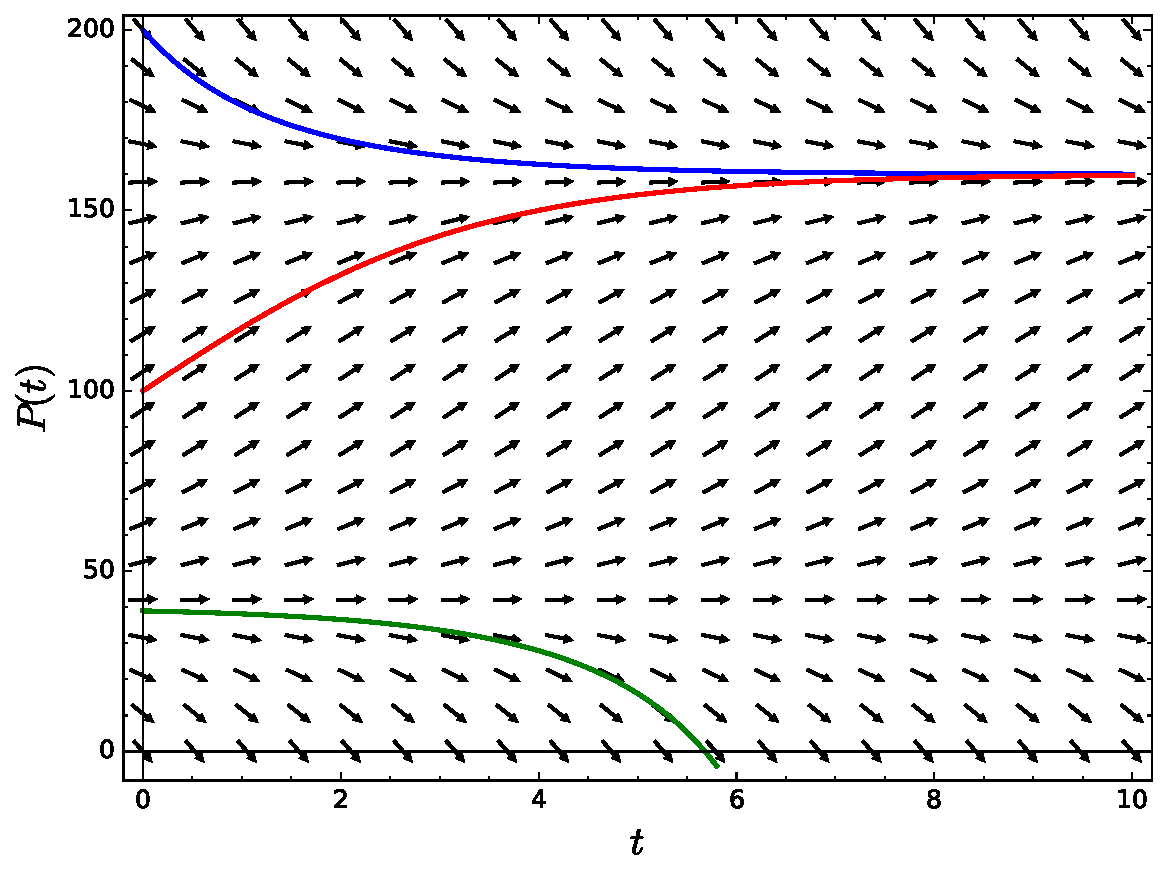
\includegraphics[width=\linewidth]{generated/sageplot/firstlook07-harvesting-sink-source.pdf}%
\end{image}%
\tcblower
\end{figureptx}%
Now let us see what happens when we allow more fishing in our pond, say \(H = 100\). Our differential equation now becomes%
\begin{equation*}
\frac{dP}{dt} = P\left(1 - \frac{P}{200} \right) - 100.
\end{equation*}
To determine the equilibrium solutions, we must solve%
\begin{equation}
\frac{dP}{dt} = P\left(1 - \frac{P}{200} \right) - 100 = 0\label{x:men:firstlook07-equation-over-harvesting}
\end{equation}
for \(P\). This last equation can be rewritten as \(P^2 - 200P + 20000 = 0\). Thus,%
\begin{equation*}
P = \frac{200 \pm \sqrt{200^2 - 4 \cdot 20000}}{2} = 100 \pm \sqrt{-10000},
\end{equation*}
which means that equation \hyperref[x:men:firstlook07-equation-over-harvesting]{({\xreffont\ref{x:men:firstlook07-equation-over-harvesting}})} has no real solutions and that we have no equilibrium solutions. Furthermore, \(dP/dt \lt 0\) for all values of \(P\).  This means that no matter how many fish are in the pond initially, the trout population will eventually die out due to overfishing  (\hyperref[x:figure:firstlook07-figure-over-harvesting]{Figure~{\xreffont\ref{x:figure:firstlook07-figure-over-harvesting}}}).%
\begin{figureptx}{Harvesting with \(H = 100\)}{x:figure:firstlook07-figure-over-harvesting}{}%
\begin{image}{0.2}{0.6}{0.2}%
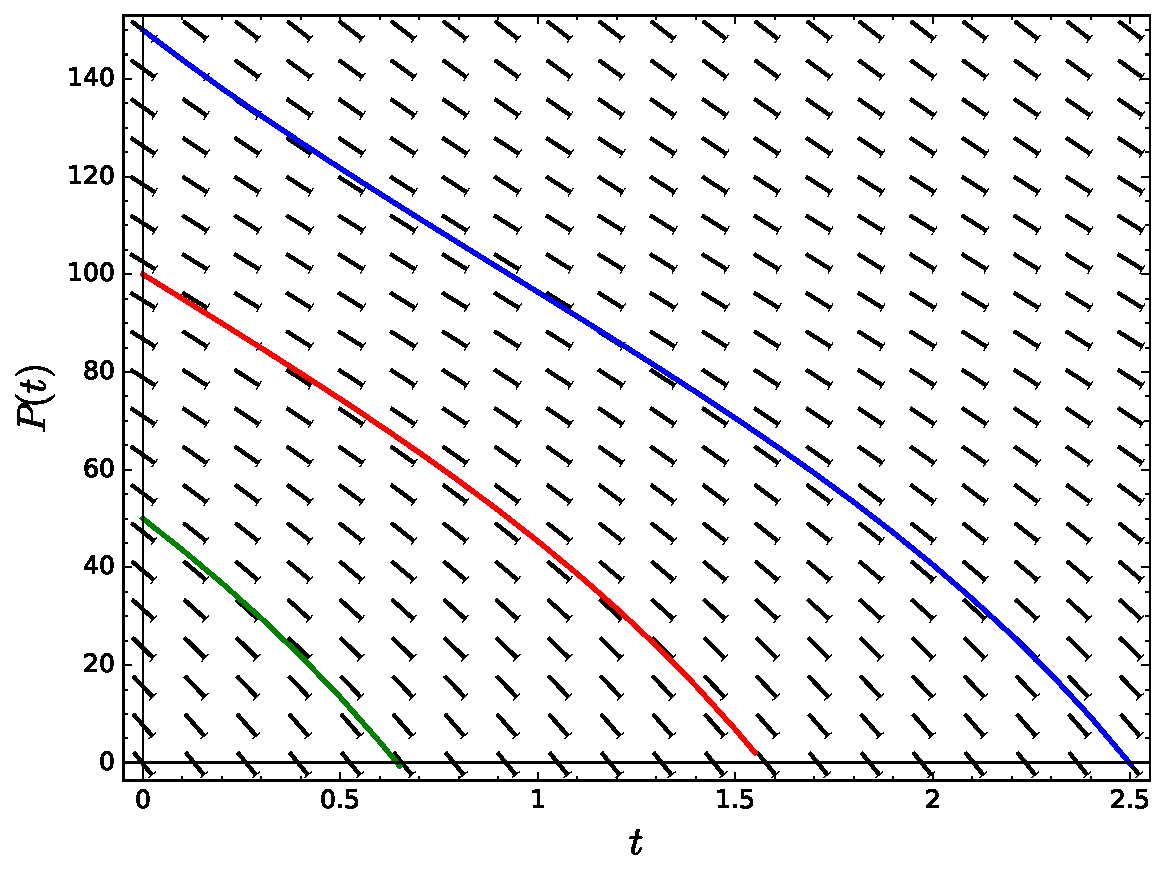
\includegraphics[width=\linewidth]{generated/sageplot/firstlook07-over-harvesting.pdf}%
\end{image}%
\tcblower
\end{figureptx}%
Finally, we will let \(H = 50\). In this case, we must solve%
\begin{equation*}
\frac{dP}{dt} = P\left(1 - \frac{P}{200} \right) - 50 = 0
\end{equation*}
in order to determine any equilibrium solutions. We now obtain a single equilibrium solution at \(P = 100\). In fact, \(P = 100\) will be a node. For values of \(P \gt 100\) as well as values of \(P \lt 100\), we have \(dP/dt \lt 0\), and the number of fish in the pond will decrease (\hyperref[x:figure:firstlook07-figure-logistic-harvesting-bifurcation]{Figure~{\xreffont\ref{x:figure:firstlook07-figure-logistic-harvesting-bifurcation}}}).%
\begin{figureptx}{Harvesting with \(H = 50\)}{x:figure:firstlook07-figure-logistic-harvesting-bifurcation}{}%
\begin{image}{0.2}{0.6}{0.2}%
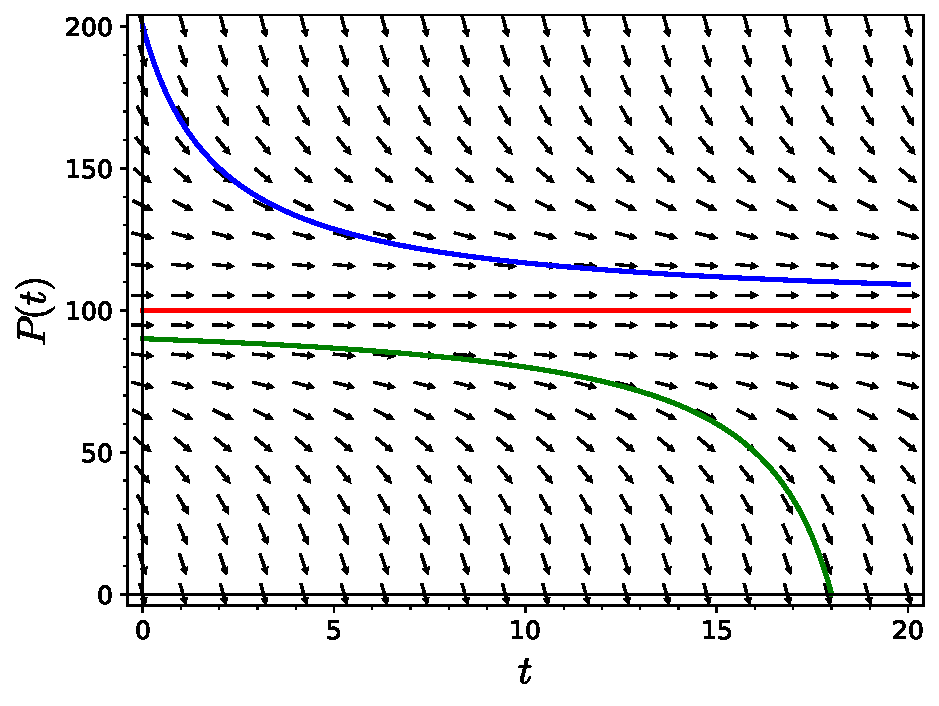
\includegraphics[width=\linewidth]{generated/sageplot/firstlook07-harvesting-bifurcation.pdf}%
\end{image}%
\tcblower
\end{figureptx}%
To better understand what is happening, we will generalize our model. Suppose that a population with a limited carrying capacity \(N\) is modeled with the logistic equation%
\begin{equation*}
\frac{dP}{dt} = kP\left(1 - \frac{P}{N}\right).
\end{equation*}
If we allow harvesting at a constant rate \(H\), our model now becomes%
\begin{equation*}
\frac{dP}{dt} = kP\left(1 - \frac{P}{N}\right) - H.
\end{equation*}
To analyze our model, we will first find the equilibrium solutions. If we will let%
\begin{equation*}
f_H(P) = kP\left(1 - \frac{P}{N}\right) - H,
\end{equation*}
each equilibrium solution must satisfy \(f_H(P) = 0\) or%
\begin{equation*}
-k P^2 + kNP - H  N = 0.
\end{equation*}
Therefore, our equilibrium solutions are given by%
\begin{equation*}
P = \frac{-kN \pm \sqrt{k^2N^2 - 4kHN}}{-2k} = \frac{N}{2} \pm  \sqrt{\frac{N^2}{4} - \frac{HN}{k}}.
\end{equation*}
%
\par
The explanation of how our model behaves lies in the discriminant,%
\begin{equation*}
\frac{N^2}{4} - \frac{HN}{k}.
\end{equation*}
If%
\begin{equation*}
\frac{N^2}{4} - \frac{HN}{k} \lt 0
\end{equation*}
or, equivalently if \(H \gt kN/4\), there are no equilibrium solutions and%
\begin{equation*}
\frac{dP}{dt} = f_H(P) \lt 0
\end{equation*}
for all values of \(P\). In particular, all solutions of \(dP/dt = f_H(P)\) tend towards negative infinity as \(t \to \infty\). In this case, the population is doomed to extinction no matter how large the initial population is. Since negative populations do not make sense, we say that the population is extinct when \(P = 0\).%
\par
On the other hand, if \(H \lt kN/4\), we have equilibrium solutions at%
\begin{equation*}
P_1 =\frac{N}{2} + \sqrt{\frac{N^2}{4} - \frac{HN}{k}}
\end{equation*}
and%
\begin{equation*}
P_2 = \frac{N}{2} - \sqrt{\frac{N^2}{4} - \frac{HN}{k}}.
\end{equation*}
The first equilibrium solution, \(P_1\) is a sink, while the second, \(P_2\) is a source.%
\par
Finally, if \(H = kN/4\), then we will have exactly one equilibrium solution at \(P = N/2\). Although \(dP/dt \lt 0\) for all \(P \neq N/2\), we see that \(P \to N/2\) as \(t \to \infty\) for all initial values of \(P\) greater than \(N/2\). For initial values of \(P\) less than \(N/2\), solutions tend towards \(- \infty\) as \(t \to \infty\). Thus, the initial population of fish must be at least \(kN/4\); otherwise, the fish will go extinct.%
\par
In our example, we have a family of differential equations\textemdash{}one for each value of \(H\),%
\begin{equation}
\frac{dP}{dt} = P\left( 1 - \frac{P}{200}\right) - H.\label{x:men:firstlook07-equation-fishing}
\end{equation}
A small change in \(H\) can have a dramatic effect on how the solutions of the differential equation behave. Changing the value of \(H\) from \(50\) to \(50.1\) will doom the population of fish to extinction no matter what the initial population is. As we increase the value of \(H\), the number of equilibrium solutions changes from two to one and then to none. This change occurs exactly at \(H = 50\). We say that a \terminology{bifurcation}\index{bifurcation} occurs at \(H = 50\) for equation \hyperref[x:men:firstlook07-equation-fishing]{({\xreffont\ref{x:men:firstlook07-equation-fishing}})}.%
\begin{activity}{Upland Bird Populations.}{g:activity:idp105545993053584}%
The chukar partridge, or simply chukar, is a upland gamebird in the pheasant family. Originally native to Asia and ranging from the eastern Mediterranean to Himalayas, the chukar has been widely introduced as an upland game bird with populations now established in the United States, Canada, Chile, Argentina, New Zealand and Hawaii. One particularly good area for hunting chukar is the western Great Basin area of the U.S. (eastern Oregon and Washington and western Idaho).%
\begin{enumerate}[font=\bfseries,label=(\alph*),ref=\alph*]
\item{}Suppose that the population of chukar on a private game ranch in eastern Oregon grows logisitically.  Estimates tell us that the one hundred square mile ranch and that the ranch can support at most \(120\) birds per square mile. The growth rate of the chukar population is estimated to be \(1.5\) birds per year. Model the growth of the chukar population with an initial value problem.%
\item{}Suppose that hunting on the ranch is restricted to guests and the average guest harvest \(10\) chukars per visit. Modify the model in part (a) to take into account the effect that hunting has on the chukar population.%
\item{}What is the maximum number of guests that the ranch can accommodate and still maintain a healthy population of game birds? How many chukar per square mile would be needed to allow this many guests?%
\end{enumerate}
\end{activity}%
\end{subsectionptx}
%
%
\typeout{************************************************}
\typeout{Subsection 1.7.2 One-Parameter Families}
\typeout{************************************************}
%
\begin{subsectionptx}{One-Parameter Families}{}{One-Parameter Families}{}{}{x:subsection:firstlook07-subsection-one-parameter-families}
Let us consider the equation%
\begin{equation}
\frac{dx}{dt} = x^2 - 4x + \lambda\label{x:men:firstlook07-equation-one-parameter-bifurcation}
\end{equation}
as a family of differential equations indexed by the parameter \(\lambda\). If we let \(f_\lambda(x) = x^2 - 4x + \lambda\), then%
\begin{equation*}
\frac{dx}{dt} = f_\lambda(x)
\end{equation*}
is a called \terminology{one-parameter family}\index{differential equation!one-parameter family} of differential equations. For each value of \(\lambda\), we obtain an autonomous differential equation, and for each value of \(\lambda\), we have a different phase line to examine.%
\par
For \(\lambda = 0\), the differential equation%
\begin{equation*}
\frac{dx}{dt} = f_0(x) = x^2 - 4x = x(x-4),
\end{equation*}
there is a sink at \(x = 0\) and a source at \(x = 4\) (\hyperref[x:figure:firstlook07-figure-one-parameter-bifurcation-0]{Figure~{\xreffont\ref{x:figure:firstlook07-figure-one-parameter-bifurcation-0}}}).%
\begin{figureptx}{\(x' = x^2 - 4x + \lambda\) for \(\lambda = 0\)}{x:figure:firstlook07-figure-one-parameter-bifurcation-0}{}%
\begin{image}{0.2}{0.6}{0.2}%
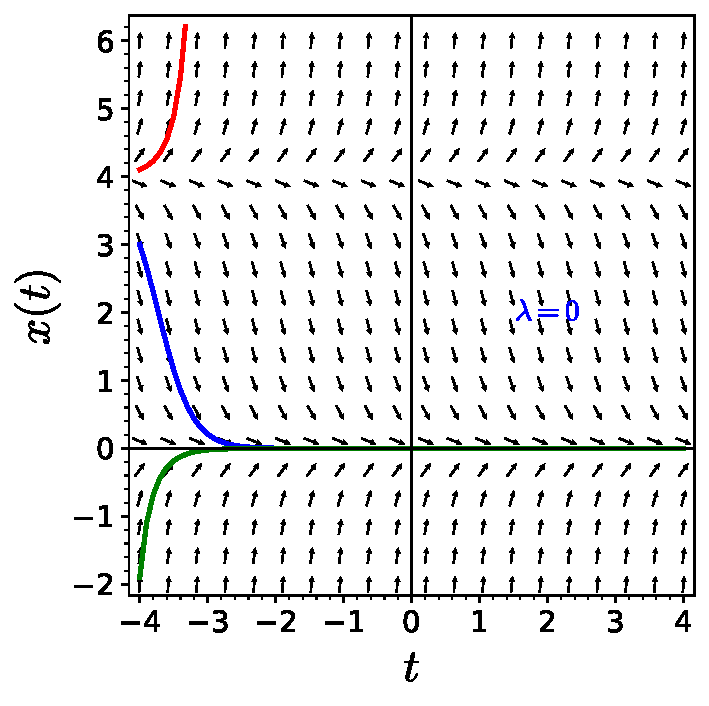
\includegraphics[width=\linewidth]{generated/sageplot/firstlook07-one-parameter-bifurcation-0.pdf}%
\end{image}%
\tcblower
\end{figureptx}%
For \(\lambda = 4\), the differential equation%
\begin{equation*}
\frac{dx}{dt} = f_4(x) = x^2 - 4x + 4 = (x - 2)^2,
\end{equation*}
we have exactly one equilibrium solution, a node at \(x = 2\) (\hyperref[x:figure:firstlook07-figure-one-parameter-bifurcation-4]{Figure~{\xreffont\ref{x:figure:firstlook07-figure-one-parameter-bifurcation-4}}}).%
\begin{figureptx}{\(x' = x^2 - 4x + \lambda\) for \(\lambda = 4\)}{x:figure:firstlook07-figure-one-parameter-bifurcation-4}{}%
\begin{image}{0.2}{0.6}{0.2}%
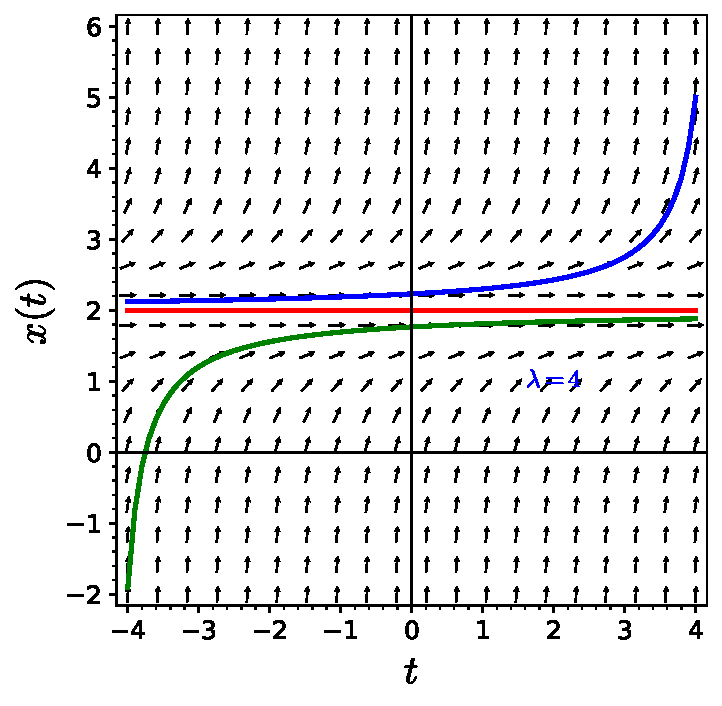
\includegraphics[width=\linewidth]{generated/sageplot/firstlook07-one-parameter-bifurcation-4.pdf}%
\end{image}%
\tcblower
\end{figureptx}%
If \(\lambda = 8\), then the differential equation%
\begin{equation*}
\frac{dx}{dt} = f_8(x) = x^2 - 4x + 8
\end{equation*}
has no equilibrium solutions (\hyperref[x:figure:firstlook07-figure-one-parameter-bifurcation-8]{Figure~{\xreffont\ref{x:figure:firstlook07-figure-one-parameter-bifurcation-8}}}).%
\begin{figureptx}{\(x' = x^2 - 2x + \lambda\) for \(\lambda = 8\)}{x:figure:firstlook07-figure-one-parameter-bifurcation-8}{}%
\begin{image}{0.2}{0.6}{0.2}%
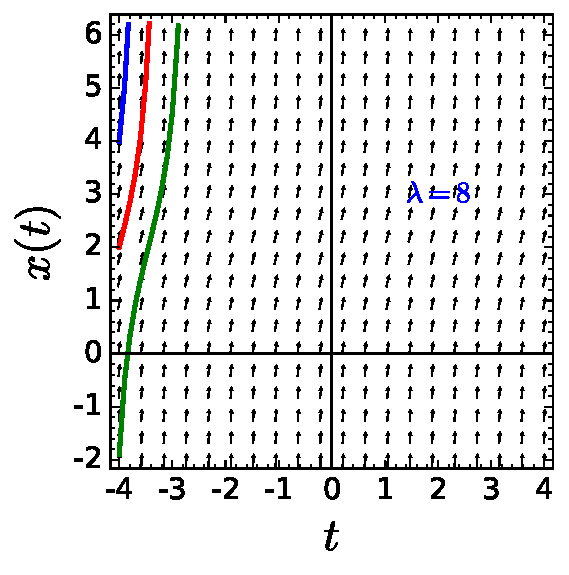
\includegraphics[width=\linewidth]{generated/sageplot/firstlook07-one-parameter-bifurcation-8.pdf}%
\end{image}%
\tcblower
\end{figureptx}%
In fact, the number of equilibrium solutions for~\hyperref[x:men:firstlook07-equation-one-parameter-bifurcation]{({\xreffont\ref{x:men:firstlook07-equation-one-parameter-bifurcation}})} changes at \(\lambda = 4\). We say that \(\lambda = 4\) is a \terminology{bifurcation value}\index{bifurcation!bifurcation value} for the differential equation%
\begin{equation}
\frac{dx}{dt} = f_\lambda(x) = x^2 - 4x + \lambda.\label{x:men:firstlook07-equation-bifurcation-1}
\end{equation}
For \(\lambda \lt 4\), we have two equilibrium solutions.%
\begin{equation*}
x = 2 \pm \sqrt{4 - \lambda}.
\end{equation*}
For values of \(\lambda \gt 4\), there are no equilibrium solutions. We can record all of the information for the various values in a graph called the \terminology{bifurcation diagram}\index{bifurcation!diagram}. The horizontal axis is \(\lambda\) and the vertical axis is \(x\). Over each value of \(\lambda\), we will plot the corresponding phase line. The curve in the graph represents the various equilibrium solutions for the different values of \(\lambda\). The bifurcation diagram for equation~\hyperref[x:men:firstlook07-equation-bifurcation-1]{({\xreffont\ref{x:men:firstlook07-equation-bifurcation-1}})} is a parabola (\hyperref[x:figure:firstlook07-figure-bifurcation-diagram]{Figure~{\xreffont\ref{x:figure:firstlook07-figure-bifurcation-diagram}}}). We have a phase line for each value of \(\lambda\).%
\begin{figureptx}{Bifurcation diagram for \(x' = x^2 - 4x + \lambda\)}{x:figure:firstlook07-figure-bifurcation-diagram}{}%
\begin{image}{0.2}{0.6}{0.2}%
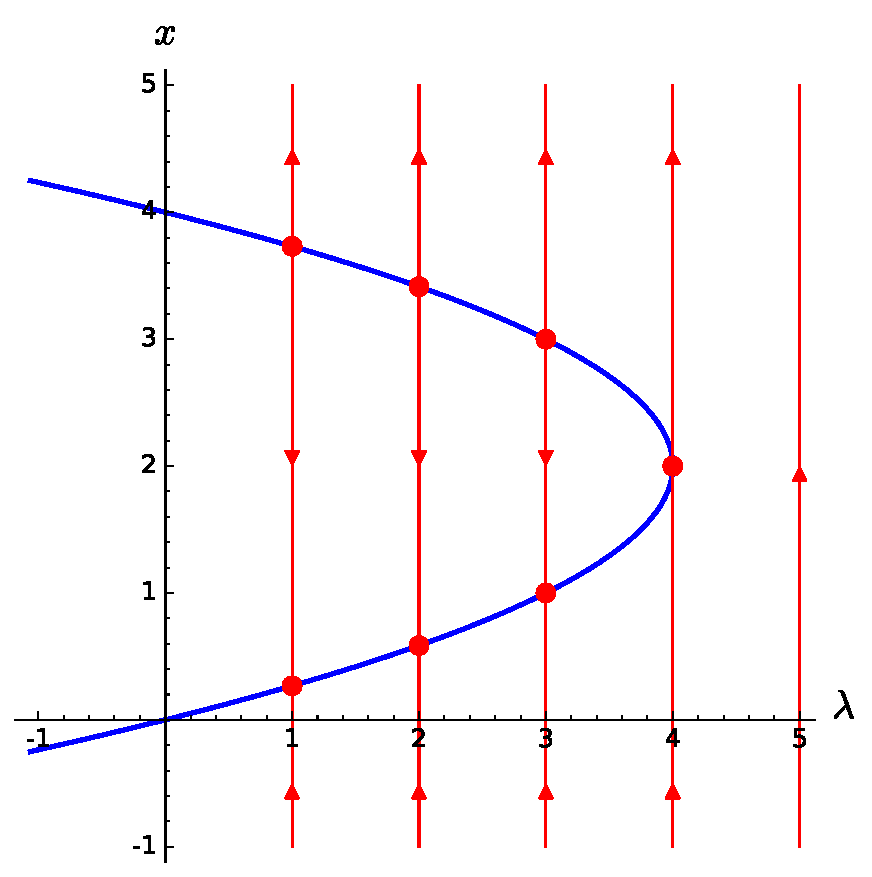
\includegraphics[width=\linewidth]{generated/sageplot/firstlook07-bifurcation-diagram.pdf}%
\end{image}%
\tcblower
\end{figureptx}%
Bifurcations for a one-parameter family of differential equations \(dx/dt = f_\lambda(x)\) are, in fact, rare. Let us consider a bifurcation where a sink changes to a source as we vary the parameter \(\lambda\). Suppose that for \(\lambda = \lambda_0\), we have a sink at \(x_0\). Then%
\begin{equation*}
\frac{dx}{dt} = f_{\lambda_0}(x_0) = 0.
\end{equation*}
Furthermore, the graph of \(f_{\lambda_0}(x)\) must be decreasing for \(x\) near \(x_0\), since \(f_{\lambda_0}(x)\) must be postive for values of \(x \lt x_0\) and negative for values of \(x \gt x_0\).  In other words, \(f'_{\lambda_0}(x) \lt 0\) for \(x\) near \(x_0\) with \(f'_{\lambda_0}(x_0) \lt 0\), then for all \(\lambda_1\) sufficiently close to \(\lambda_0\), the differential equation%
\begin{equation*}
\frac{dx}{dt} = f_{\lambda_1}(x)
\end{equation*}
must have sink at a point \(x = x_1\) very close to \(x_0\).  A similar situation holds if \(x_0\) is a source and \(f'_{\lambda_0}(x_0) \gt 0\). Thus, bifurcations can only occur when \(f_{\lambda_0}(x_0) = 0\) and \(f'_{\lambda_0}(x_0) = 0\).%
\begin{example}{}{g:example:idp105545993092368}%
Now consider the one-parameter family%
\begin{equation*}
\frac{dy}{dt}  = y^3 - \alpha y = y (y^2 - \alpha).
\end{equation*}
We will have an equilibrium solution at zero for all values of \(\alpha\) and two additional equilibrium solutions at \(\pm \sqrt{\alpha}\) for \(\alpha \gt 0\).  This type of  bifurcation is a \terminology{pitch fork bifurcation}\index{bifurcation!pitch fork} (\hyperref[x:figure:firstlook07-figure-bifurcation-pitchfork]{Figure~{\xreffont\ref{x:figure:firstlook07-figure-bifurcation-pitchfork}}}).%
\begin{figureptx}{The bifurcation diagram for \(y' = y^3 - \alpha y\)}{x:figure:firstlook07-figure-bifurcation-pitchfork}{}%
\begin{image}{0.2}{0.6}{0.2}%
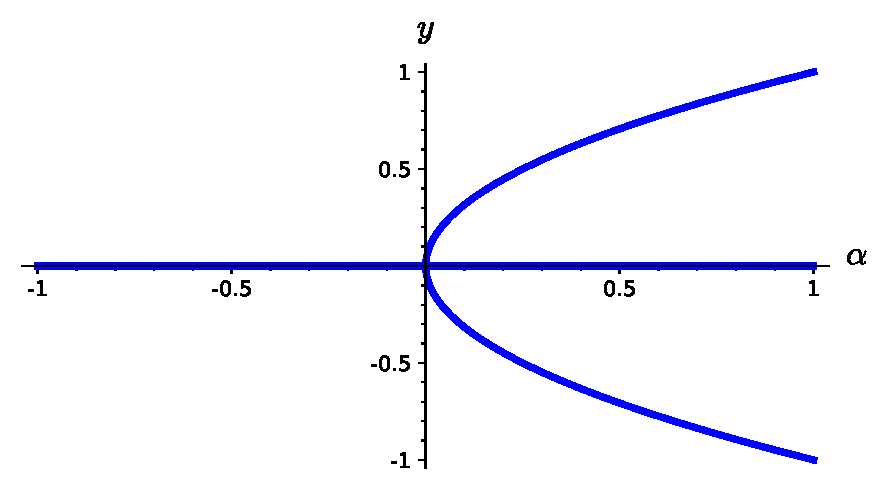
\includegraphics[width=\linewidth]{generated/sageplot/firstlook07-bifurcation-pitchfork.pdf}%
\end{image}%
\tcblower
\end{figureptx}%
\end{example}
\begin{activity}{Bifurcations.}{g:activity:idp105545993064592}%
For each of the following parametrized family of differential equations, plot phase lines for \(c = -2, -1, 0, 1, 2\), find any bifurcation values, and sketch the bifurcation diagram.%
\begin{enumerate}[font=\bfseries,label=(\alph*),ref=\alph*]
\item{}\(y' = (1 - y)y + c\)%
\item{}\(y' = (c - y^2)y\)%
\end{enumerate}
\end{activity}%
\begin{example}{}{g:example:idp105545993067024}%
Let us find the bifurcation values of the one-parameter family%
\begin{equation}
\frac{dy}{dt}  = y(y - 2)^2 + \lambda.\label{x:men:firstlook07-equation-bifurcation-2}
\end{equation}
If \(g_\lambda(y) = y(y - 2)^2 + \lambda\), then \(g'_\lambda(y) =  3y^2 - 8y + 4\). The roots of \(g'_\lambda(y) = 0\) are \(y = 2\) and \(y = 2/3\). In order for \(\lambda\) to be a bifurcation value, we must have  \(g_\lambda(2) = \lambda = 0\) or%
\begin{equation*}
g_\lambda(2/3) = \frac{32}{27} + \lambda = 0 
\end{equation*}
Thus, equation~\hyperref[x:men:firstlook07-equation-bifurcation-2]{({\xreffont\ref{x:men:firstlook07-equation-bifurcation-2}})} has two bifurcation values, \(\lambda = -32/27\) and \(\lambda = 0\). The bifurcation diagram for this one-parameter family is given in \hyperref[x:figure:firstlook07-figure-two-bifurcations]{Figure~{\xreffont\ref{x:figure:firstlook07-figure-two-bifurcations}}}.%
\begin{figureptx}{The bifurcation diagram for \(y' =  y(1 - y)^2 + \lambda\)}{x:figure:firstlook07-figure-two-bifurcations}{}%
\begin{image}{0.2}{0.6}{0.2}%
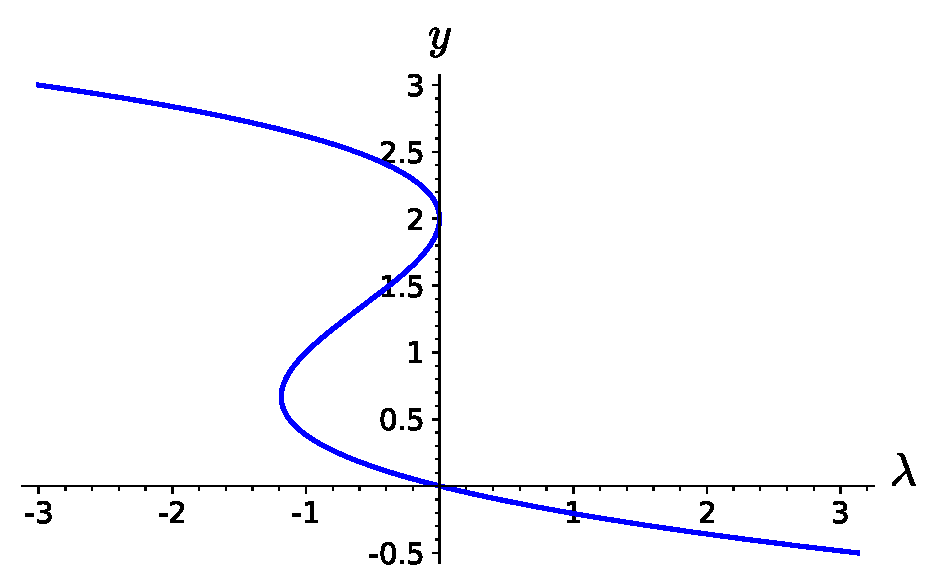
\includegraphics[width=\linewidth]{generated/sageplot/firstlook07-two-bifurcations.pdf}%
\end{image}%
\tcblower
\end{figureptx}%
\end{example}
\end{subsectionptx}
%
%
\typeout{************************************************}
\typeout{Subsection 1.7.3 Important Lessons}
\typeout{************************************************}
%
\begin{subsectionptx}{Important Lessons}{}{Important Lessons}{}{}{x:subsection:firstlook07-subsection-important-lessons}
%
\begin{itemize}[label=\textbullet]
\item{}A one-parameter family of differential equations%
\begin{equation*}
\frac{dx}{dt} = f_\lambda(x)
\end{equation*}
has a bifurcation at \(\lambda = \lambda_0\) if a change in the number of equilibrium solutions occurs.%
\item{}Bifurcation diagrams are an effective way of representing the nature of the solutions of a one-parameter family of differential equations.%
\item{}Bifurcations for a one-parameter family of differential equations \(dx/dt = f_\lambda(x)\) are rare. Bifurcations occur when \(f_{\lambda_0}(x_0) = 0\) and \(f'_{\lambda_0}(x_0) = 0\).%
\end{itemize}
%
\end{subsectionptx}
%
%
\typeout{************************************************}
\typeout{Reading Questions 1.7.4 Reading Questions}
\typeout{************************************************}
%
\begin{reading-questions-subsection}{Reading Questions}{}{Reading Questions}{}{}{x:reading-questions:reading-questions-firstlook07}
\begin{divisionexercise}{1}{}{}{x:exercise:reading-questions-firstlook07-1}%
Explain what a bifurcation is in your own words.%
\end{divisionexercise}%
\begin{divisionexercise}{2}{}{}{x:exercise:reading-questions-firstlook07-2}%
Explain why a bifurcation is relatively rare for a one-parameter family of differential equations.%
\end{divisionexercise}%
\end{reading-questions-subsection}
%
%
\typeout{************************************************}
\typeout{Exercises 1.7.5 Exercises}
\typeout{************************************************}
%
\begin{exercises-subsection}{Exercises}{}{Exercises}{}{}{x:exercises:firstlook07-exercises}
\begin{divisionexercise}{1}{}{}{g:exercise:idp105545993114000}%
For each of the following parametrized family of differential equations, plot phase lines for \(\lambda = -2, -1, 0, 1, 2\), find any bifurcation values, and sketch the bifurcation diagram.%
\begin{enumerate}[label=(\alph*)]
\item{}\(y' = \lambda - y^2\).%
\item{}\(y' = \lambda y^2 - 1\) for \(\lambda \in {\mathbb R}\).%
\item{}\(y' = \lambda - 2y + y^2\).%
\item{}\(y' = (\lambda - 4y^2)y\).%
\item{}\(y' = (\lambda - y^4)y\).%
\end{enumerate}
%
\end{divisionexercise}%
\begin{divisionexercise}{2}{}{}{g:exercise:idp105545993118608}%
Describe the phase line portraits for \(y' = \lambda y - \sin y\) for \(\lambda > 2 / \pi\) and how it depends on the parameter \(\lambda\). Draw the bifurcation diagram for this equation.%
\end{divisionexercise}%
\begin{divisionexercise}{3}{}{}{g:exercise:idp105545993120400}%
The differential equation%
\begin{equation*}
\frac{dy}{dt} = y - 4t + y^2 - 8yt + 16 t^2 + 4.
\end{equation*}
is not autonomous, separable, or linear; however, we can solve this equation with a change of variable.%
\begin{enumerate}[label=(\alph*)]
\item{}Transform this equation into a new differential equation of the form%
\begin{equation*}
\frac{du}{dt}= f(u)
\end{equation*}
by letting \(u = y - 4t\).%
\item{}Sketch the phase line for this new equation, \(u' = f(u)\), and sketch several solutions.%
\item{}Find the solutions of the original differential equation that correspond to the equilibrium solutions of \(u' = f(u)\). Graph these solutions in \(ty\)-plane.  Also, sketch the graphs of the solutions that you plotted in part (b).%
\item{}Solve the differential new equation and use this information to solve the original differential equation.%
\end{enumerate}
%
\end{divisionexercise}%
\end{exercises-subsection}
\end{sectionptx}
%
%
\typeout{************************************************}
\typeout{Section 1.8 Projects for First-Order Differential Equations}
\typeout{************************************************}
%
\begin{sectionptx}{Projects for First-Order Differential Equations}{}{Projects for First-Order Differential Equations}{}{}{x:section:firstlook08}
\begin{project}{Project\textemdash{}The Spruce Budworm.}{x:project:firstlook08-project-spruce-budworm}%
\emph{Choristoneura fumiferana} or the \emph{eastern spruce budworm} is a species of moth native to the eastern United States and Canada. The caterpillars feed on the needles of spruce and fir trees. Populations can experience significant oscillations.  The spruce budworm population remains at a relatively low, constant level most of the time.  However, outbreaks have been recurring approximately every three decades, and studies suggest the spruce budworm has been breaking out in eastern North America for thousands of years.%
\par
Outbreaks of the spruce budworm have been responsible for some major deforestations in Canada and the United States. The eastern spruce budworm is considered one of the most destructive forest pests in North America.%
\par
You are acting as a consultant to the state department of forestry.  Your task is to explain how outbreaks occur and how often the state can expect outbreaks.%
\par
The equation%
\begin{equation}
x' = r \left( 1 - \frac{x}{K} \right) x - c \frac{x^2}{a + x^2}\label{x:men:firstlook08-equation-spruce-budworm}
\end{equation}
has been used to describe the dynamics of spruce budworm populations, where the variable \(x\) denotes the population or density of the insect~\hyperlink{x:biblio:ludwig-1978}{[{\xreffont 16}]}.  One explanation that has been given for the occurrence of outbreaks is based on the multiple bifurcations that occur with this differential equation.%
\begin{enumerate}[font=\bfseries,label=(\alph*),ref=\alph*]
\item{}Explain how \hyperref[x:men:firstlook08-equation-spruce-budworm]{({\xreffont\ref{x:men:firstlook08-equation-spruce-budworm}})} can be used to model the spruce budworm population.%
\item\label{x:task:firstlook08-task-spruce-budworm-ii}If \(a = 0.01\), \(c = 1\), and \(K = 1\), we have a family of differential equations parameterized by \(r\),%
\begin{equation*}
x' = rx(1-x) - \frac{x^2}{0.01 + x^2}.
\end{equation*}
Solve the equation%
\begin{equation*}
rx(1-x) - \frac{x^2}{0.01 + x^2} = 0
\end{equation*}
and plot the result in the \(xr\)-plane for \(0 \leq r \lt 1\).%
\item{}To find the bifurcation diagram for the spruce budworm equation, reflect the graph obtained in part \hyperref[x:task:firstlook08-task-spruce-budworm-ii]{Task~{\xreffont\ref{x:project:firstlook08-project-spruce-budworm}}.{\xreffont\ref{x:task:firstlook08-task-spruce-budworm-ii}}} about the line \(r= x\) line.%
\item{}Estimate the two bifurcation values from your graph. Explain what happens to the population as \(r\) increases. That is, when does an outbreak occur?  What happens after an outbreak?%
\item{}\lititle{Your Final Report.}\par%
Your final report should contain a one-page executive summary.  The executive summary should summarize your work in such a way that the reader can rapidly become acquainted with the material. It should contain a brief description of the problem, important background information, a discussion of pertinent assumptions, a short description of your methodology, concise analysis, and your main conclusions. Assume the reader is familiar with the basics of calculus and differential equations, so there is no need to walk through every step of your solution process or include equations. However, you should still describe the processes and mathematical techniques you used to reach your conclusions and explain why you used them.  Refer the reader to the appendices as needed.%
\par
Appendices should be neatly formatted and present information in a logical manner. \emph{DO NOT} simply print out Sage code. Consolidate your results and provide a short explanation of what it is the reader is seeing while also highlighting key pieces of information in the appendix.%
\begin{itemize}[label=\textbullet]
\item{}Appendix A\textemdash{}Answers and analysis%
\item{}Additional Appendices\textemdash{}Include additional appendices as necessary.%
\end{itemize}
%
\end{enumerate}
\end{project}%
\begin{project}{Project\textemdash{}The Spread of an Oil Spill.}{x:project:firstlook08-project-oil-spill}%
Oil spills such as the Deepwater Horizon in the Gulf of Mexico or the Amoco Cadiz off the coast of Brittany can have disastrous consequences for society\textemdash{}economically, environmentally, and socially. Even smaller spills such as the Exxon Valdez can have have a huge impact on the surrounding environment due to the remoteness of the site or the difficulty of mounting an emergency environmental response.  Cleanup and recovery from an oil spill is difficult and depends upon many factors, including the type of oil spilled, the temperature of the water, and the types of shorelines and beaches involved. Spills may take weeks, months or even years to clean up.  For this reason the timeliness of an emergency response is critical.\footnotemark{}%
\par
Suppose an oil spill occurs off the coast of Texas. From time to time, but irregularly, a helicopter is dispatched by the Coast Guard to photograph the oil slick. On each trip, the helicopter arrives over the slick, the pilot takes a photo, waits 10 minutes, takes a second photo, and heads home. On each of seven trips the size (in area) of the slick is measured from both photographs.  The data is given in \hyperref[x:table:firstlook08-table-oil-spill]{Table~{\xreffont\ref{x:table:firstlook08-table-oil-spill}}}%
\begin{tableptx}{\textbf{Data on spread of an oil spill}}{x:table:firstlook08-table-oil-spill}{}%
\centering%
{\tabularfont%
\begin{tabular}{cc}\hrulemedium
Initial Observation&10 Minutes Later\tabularnewline\hrulemedium
1.047&1.139\tabularnewline[0pt]
2.005&2.087\tabularnewline[0pt]
3.348&3.413\tabularnewline[0pt]
5.719&5.765\tabularnewline[0pt]
7.273&7.304\tabularnewline[0pt]
8.410&8.426\tabularnewline[0pt]
9.117&9.127\tabularnewline\hrulemedium
\end{tabular}
}%
\end{tableptx}%
\begin{enumerate}[font=\bfseries,label=(\alph*),ref=\alph*]
\item{}Build a model for the size of the oil slick at time \(t\).%
\item{}Predict the future size of the oil slick, say at \(t=10\) min, \(t=20\) min, \(t=120\) min.%
\item{}Plot your model of the size of the oil slick as a function of time.%
\item{}Find the time at which the oil slick is 8 square miles.%
\item{}Determine the time of each of the observations for the first, third, fifth, and seventh initial observations.%
\item{}\lititle{Your Final Report.}\par%
You have been retained as a consultant to the  United States Coast Guard (USCG) to analyze this data and submit a report of your findings.  Your final report should contain a one-page executive summary.  The executive summary should summarize your work in such a way that the reader can rapidly become acquainted with the material. It should contain a brief description of the problem, important background information, a discussion of pertinent assumptions, a short description of your methodology, concise analysis, and your main conclusions. Do not assume that the reader knows anything about calculus or differential equations, but does have experts that can verify your model and calculations, which should appear in an appendix.%
\par
Appendices should be neatly formatted and present information in a logical manner. \emph{DO NOT} simply print out Sage code or a series of equations. Consolidate your results and provide a short explanation of what it is the reader is seeing while also highlighting key pieces of information in the appendix.%
\begin{itemize}[label=\textbullet]
\item{}Appendix A\textemdash{}Answers and analysis%
\item{}Additional Appendices\textemdash{}Include additional appendices as necessary.%
\end{itemize}
%
\end{enumerate}
\end{project}%
\footnotetext[1]{This project is adapted from Brian Winkel(2015), ``1-005-S-OilSlick,'' \href{https://www.simiode.org/resources/196}{\nolinkurl{https://www.simiode.org/resources/196}}.\label{g:fn:idp105545993108880}}%
\begin{project}{Project\textemdash{}Malaria Control.}{x:project:firstlook08-malaria-control}%
Your company has been contracted to build a hospital in sub-Saharan Africa. The company is aware of the malaria threat in the region and has asked you to analyze malaria preventive measures for the employees that will be sent to build the hospital.\footnotemark{}%
\par
Malaria is a serious and sometimes fatal disease. In 2018, it was estimated that 228 million people worldwide contracted malaria.  The estimated number of deaths was approximately 405,000 people. Children under the age of 5 years are the most vulnerable group, and they accounted for 67\% (272,000) of all malaria deaths worldwide. Ninety-three percent of malaria cases are in Africa with six countries accounting or more than half of all malaria cases worldwide: Nigeria (25\%), the Democratic Republic of the Congo (12\%), Uganda (5\%), and Côte d’Ivoire, Mozambique and Niger (4\% each).\footnotemark{}%
\par
People who get malaria are typically very sick with high fevers, shaking chills, and flu-like illness. Although malaria can be a deadly disease, illness and death from malaria can usually be prevented. The disease is caused by a parasite that infects red blood cells. The parasite is transmitted from person to person through the bite of mosquitoes. Avoiding mosquito bites is the only sure method to prevent malaria infection. Malaria can be cured with prescription drugs. The type of drugs and length of treatment depend on the type of malaria, where the person was infected, their age, whether they are pregnant, and how sick they are at the start of treatment.\footnotemark{}%
\begin{enumerate}[font=\bfseries,label=(\alph*),ref=\alph*]
\item\label{x:task:firstlook08-task-pharmacokinetics}\lititle{Pharmacokinetics of Malaria Chemoprophylaxis.}\par%
Your first task is to analyze the anti-malarial drug dosing regimen for those building the hospital. The primary concerns are how soon to start treatment before everyone arrives and the potential risks if employees miss one or two of their scheduled doses. These questions require an understanding of pharmacokinetics.%
\par
Pharmacokinetics is the study of what the body does to a drug. Specifically, it refers to the movement of the drug into, through, and out of the body. Understanding the pharmacokinetics of a drug allows medical professionals to develop appropriate drug dosing regimens for their patients.  A complete understanding of the pharmacokinetics of a drug requires information on the processes of absorption, distribution, metabolization, and excretion of the drug from the body. In order to simplify this problem, we will assume that the anti-malarial medication is immediately absorbed into the blood stream and that everyone begins treatment with zero anti-malarial medication in their body. After the drug is absorbed into the blood, the rate of elimination of the drug from the body is proportional to the amount of drug currently in the blood. In other words, the more of the drug in the blood stream, the faster it is removed from the body. We will also assume that the rate of excretion of the drug is the same for everyone.%
\par
Atovaquone\slash{}proguanil, sold under the trade names Malarone among others, is a combination of two antimalarial medication atovaquone and proguanil. It is used to treat and prevent malaria, including chloroquine-resistant malaria.  A standard adult pill of Malarone contains 250mg of atovaquone and 100mg of proguanil. A typical dose is one pill taken at the same time each day. An individual must maintain at least 300mg of atovaquone and 30mg of proguanil in their blood at all times in order to prevent contracting malaria. A typical adult eliminates atovaquone at a rate that corresponds to a half-life (time to eliminate one half of the original dose) of 48 hours. The half-life of proguanil is 12 hours.\footnotemark{}%
\begin{enumerate}[font=\bfseries,label=(\roman*),ref=\theenumi.\roman*]
\item\label{x:task:firstlook08-task-malarone-i}At \(t = 0\), a typical adult ingests one pill of Malarone. Write an initial value problem (IVP) that models the mass (mg) of the drug proguanil in the adult's blood for \(t \geq 0\). Solve this IVP analytically. After a person takes the first pill of Malarone, if they take no further medication, for how many hours can they expect to have enough proguanil in his blood to prevent contracting malaria?%
\item\label{x:task:firstlook08-task-malarone-ii}Approximate the solution to the IVP you developed in \hyperref[x:task:firstlook08-task-malarone-i]{Task~{\xreffont\ref{x:project:firstlook08-malaria-control}}.{\xreffont\ref{x:task:firstlook08-task-malarone-i}}} over the next seven days (168 hours) by implementing Euler’s method in Sage with two step sizes: \(h = 6\) hours and \(h = 1\) hour (see \href{http://utmost-sage-cell.org/diff-equations}{\nolinkurl{utmost-sage-cell.org/diff-equations}}). Compute the error for both step sizes by comparing your estimate to the analytic solution.%
\begin{sageinput}

\end{sageinput}
\begin{sageoutput}

\end{sageoutput}
\item\label{x:task:firstlook08-task-malarone-iii}Approximate the solution to the IVP over the next seven days by implementing the RK4 or classic Runge–Kutta method in Sage with step size: \(h = 1\) hour. Compute the error for both step sizes by comparing your estimate to the analytic solution (see \href{http://utmost-sage-cell.org/diff-equations}{\nolinkurl{utmost-sage-cell.org/diff-equations}}).%
\begin{sageinput}

\end{sageinput}
\begin{sageoutput}

\end{sageoutput}
\item\label{x:task:firstlook08-task-malarone-iv}Create a table summarizing the results of all numerical methods (\hyperref[x:task:firstlook08-task-malarone-ii]{Task~{\xreffont\ref{x:project:firstlook08-malaria-control}}.{\xreffont\ref{x:task:firstlook08-task-malarone-ii}}} and \hyperref[x:task:firstlook08-task-malarone-iii]{Task~{\xreffont\ref{x:project:firstlook08-malaria-control}}.{\xreffont\ref{x:task:firstlook08-task-malarone-iii}}}). This table should include columns for time, the actual mass of proguanil in each subject's blood (from \hyperref[x:task:firstlook08-task-malarone-i]{Task~{\xreffont\ref{x:project:firstlook08-malaria-control}}.{\xreffont\ref{x:task:firstlook08-task-malarone-i}}}), and the approximate values of the solution for all methods and step sizes at \(t = 0, 24, 48, \ldots, 168\) only. Your table should have a total of 5 columns. Include an additional entry at the bottom of each of the last 3 columns providing the error for that method and step size. Discuss your results. Your analysis should include a comparison of error for different step sizes and for different methods.%
\item\label{x:task:firstlook08-task-malarone-v}Write an IVP that models the mass (mg) of the drug atovaquone in a typical adult’s blood for \(t \geq 0\) if a person ingests only one pill of Malarone at \(t = 0\). Approximate the solution to this IVP using the RK4 method in Sage with step size: \(h = 1\) hour.%
\begin{sageinput}

\end{sageinput}
\begin{sageoutput}

\end{sageoutput}
\item{}Using your solutions to parts \hyperref[x:task:firstlook08-task-malarone-iii]{Task~{\xreffont\ref{x:project:firstlook08-malaria-control}}.{\xreffont\ref{x:task:firstlook08-task-malarone-iii}}} and \hyperref[x:task:firstlook08-task-malarone-v]{Task~{\xreffont\ref{x:project:firstlook08-malaria-control}}.{\xreffont\ref{x:task:firstlook08-task-malarone-v}}}, if an adult ingests one pill of Malarone at the same time each day, how long before your construction crew departure to Africa should your crew begin taking their pills? In other words, how long until everyone has enough proguanil AND atovaquone in their blood to prevent contracting malaria? Illustrate your result using a graph or table.%
\item{}Assume a typical person reaches a ``steady state'' level of proguanil and atovaquone in their body after their 8th dose of Malarone. If after reaching ``steady state'' a person misses one dose, are they at risk of contracting malaria? How about after missing two consecutive doses? Explain.%
\end{enumerate}
\item\label{x:task:firstlook08-task-population-control}\lititle{Mosquito Population Control.}\par%
Unfortunately anti-malarial drugs are not 100\% effective at preventing the spread of malaria. The only sure method to prevent contracting malaria is to avoid mosquito bites. In light of this, you must look at methods to control the mosquito population in the construction area near the living quarters. Your objective is to reduce the mosquito population in both the short (less than 6 months) and long (greater than 6 months) term while also minimizing the environmental impact and potential health problems associated with the mosquito control measures that are implemented.%
\par
There are two typical approaches to mosquito control. The first approach is to directly kill mosquitoes using an insecticide spray. The effectiveness of this method depends on the frequency of spraying and the concentration of the insecticide. However, frequent spraying of insecticide has potential negative health effects on both humans and nearby wildlife. This method is also temporary as the mosquito population will recover once routine spraying has stopped. The second approach to mosquito population control is to eliminate the resources that support the mosquito population. This is done through the destruction of mosquito breeding grounds and involves everything from filling in small puddles to the draining of swamps and marshes. Keeping in consideration manpower and budget constraints, you must find the combination of these two approaches that best meets these objectives over the next six months.%
\par
Studies on mosquito control indicate that the rate of change of the mosquito population, \(P\), (measured in millions of mosquitoes) in the area can be accurately modeled using the following Initial Value Problem:%
\begin{equation*}
\frac{dP}{dt} = kP \left( 1 - \frac{P}{M} \right) - EP, \quad P(0) = P_0,
\end{equation*}
where \(E\) is a constant that represents the effectiveness of insecticide spraying efforts, M is the local carrying capacity and is affected by efforts to reduce mosquito breeding grounds, \(k\) is the population growth constant, \(P_0\) is the initial population, and time \(t\) is measured in months. Current estimates suggest that there are approximately 10 million mosquitoes living near the proposed site of the hospital. Data indicates that \(M = 11\) million and \(k = 1.2\) for this mosquito population.%
\par
Use the information provided and the RK4 method to evaluate the following three mosquito population scenerios. Recommend a scenerio and support your recommendation with mathematics. Be sure to include other considerations (not just what your mathematical model tells you) in your analysis. Tables, graphs, and other visual representations that summarize and support your analysis and recommendation are encouraged and should be included in an appendix.%
\begin{enumerate}[font=\bfseries,label=(\roman*),ref=\theenumi.\roman*]
\item{}\lititle{Scenerio A.}\par%
In this scenerio, you would devote most of your available resources for mosquito control to the use of insecticide. You would spray highly concentrated and expensive insecticide in the employee living areas daily. Due to the emphasis on the use of insecticide would be limited to destroying small mosquito breeding grounds only on the base camp. You estimate a value for \(E\) of \(E_A\) (see \hyperref[x:table:firstlook08-table-mosquito]{Table~{\xreffont\ref{x:table:firstlook08-table-mosquito}}}) and a new carrying capacity of \(M_A\) million mosquitoes that would be in effect immediately.%
\begin{tableptx}{\textbf{Values for \(M\) and \(E\)}}{x:table:firstlook08-table-mosquito}{}%
\centering%
{\tabularfont%
\begin{tabular}{ccccccc}\hrulemedium
&\multicolumn{2}{c}{Scenerio A}&\multicolumn{2}{c}{Scenerio B}&\multicolumn{2}{c}{Scenerio C}\tabularnewline\hrulemedium
&\(M_A\)&\(E_A\)&\(M_B\)&\(E_B\)&\(M_C\)&\(E_C\)\tabularnewline\hrulemedium
Set 1&10.5&0.55&6.0&0.10&9.0&0.40\tabularnewline[0pt]
Set 2&10.0&0.60&5.5&0.10&8.5&0.45\tabularnewline[0pt]
Set 3&10.5&0.50&6.5&0.10&9.0&0.40\tabularnewline\hrulemedium
\end{tabular}
}%
\end{tableptx}%
\item{}\lititle{Scenerio B.}\par%
In this scenerio, you would devote most of your resources towards destroying mosquito breeding grounds. This would involve the permanent draining of a nearby marsh that is believed to be the primary breeding ground for mosquitoes at the construction site. Draining the marsh would take time to complete, delaying any impact on the mosquito population by two months, but would lower the carrying capacity to \(M_B\) million mosquitoes. You would still spray insecticide but less frequently and with less potency than in Scenerio A. It is estimated that spraying would immediately result in a value for \(E\) of \(E_B.\)%
\item{}\lititle{Scenerio C.}\par%
This scenerio seeks to balance the insecticide and breeding ground destruction approaches. You would use the same, more potent, insecticide as Scenerio A but spray less frequently. This would free up manpower to destroy small mosquito breeding grounds. You estimate a new value for \(E\) of \(E_C\) and a new carrying capacity of \(M_C\) million mosquitoes that would be in effect immediately.%
\end{enumerate}
\item{}\lititle{Your Final Report.}\par%
Your final report should contain a one-page executive summary.  The executive summary should summarize your work for \hyperref[x:task:firstlook08-task-pharmacokinetics]{Task~{\xreffont\ref{x:project:firstlook08-malaria-control}}.{\xreffont\ref{x:task:firstlook08-task-pharmacokinetics}}} and  \hyperref[x:task:firstlook08-task-population-control]{Task~{\xreffont\ref{x:project:firstlook08-malaria-control}}.{\xreffont\ref{x:task:firstlook08-task-population-control}}} in such a way that the reader can rapidly become acquainted with the material. It should contain a brief description of the problem, important background information, a discussion of pertinent assumptions, a short description of your methodology, concise analysis, and your main conclusions. Assume the reader is familiar with the basics of calculus and differential equations, so there is no need to walk through every step of your solution process or include equations. However, you should still describe the processes and mathematical techniques you used to reach your conclusions and explain why you used them.  Refer the reader to the appendices as needed.%
\par
Appendices should be neatly formatted and present information in a logical manner. \emph{DO NOT} simply print out Sage code. Consolidate your results and provide a short explanation of what it is the reader is seeing while also highlighting key pieces of information in the appendix.%
\begin{itemize}[label=\textbullet]
\item{}Appendix A\textemdash{}Answers and analysis for \hyperref[x:task:firstlook08-task-pharmacokinetics]{Task~{\xreffont\ref{x:project:firstlook08-malaria-control}}.{\xreffont\ref{x:task:firstlook08-task-pharmacokinetics}}}%
\item{}Appendix B\textemdash{}Provide a table that summarizes the results of your analysis for all three scenerios in \hyperref[x:task:firstlook08-task-population-control]{Task~{\xreffont\ref{x:project:firstlook08-malaria-control}}.{\xreffont\ref{x:task:firstlook08-task-population-control}}}. Also include a copy of all work you used to analyze your recommended scenerio.%
\item{}Additional Appendices\textemdash{}Include additional appendices as necessary.%
\end{itemize}
%
\end{enumerate}
\end{project}%
\footnotetext[2]{This project is adapted from David Culver (2016), ``1-024-S-MalariaControl,'' \href{https://www.simiode.org/resources/1750}{\nolinkurl{www.simiode.org/resources/1750}}.\label{g:fn:idp105545992895760}}%
\footnotetext[3]{World Malaria Report 2019, World Health Organization, \href{https://www.who.int/publications/i/item/9789241565721}{\nolinkurl{www.who.int/publications/i/item/9789241565721}}.\label{g:fn:idp105545992897168}}%
\footnotetext[4]{Malaria, Centers for Disease Control and Prevention, \href{https://www.cdc.gov/parasites/malaria/index.html}{\nolinkurl{www.cdc.gov/parasites/malaria/index.html}}.\label{g:fn:idp105545992898192}}%
\footnotetext[5]{Malarone: Prescribing Information. US Food and Drug Administration. \href{https://www.accessdata.fda.gov/drugsatfda_docs/label/2008/021078s016lbl.pdf}{\nolinkurl{www.accessdata.fda.gov/drugsatfda_docs/label/2008/021078s016lbl.pdf}}\label{g:fn:idp105545992867600}}%
\end{sectionptx}
\end{chapterptx}
%
%
\typeout{************************************************}
\typeout{Chapter 2 Systems of Differential Equations}
\typeout{************************************************}
%
\begin{chapterptx}{Systems of Differential Equations}{}{Systems of Differential Equations}{}{}{x:chapter:systems}
%
%
\typeout{************************************************}
\typeout{Section 2.1 Modeling with Systems}
\typeout{************************************************}
%
\begin{sectionptx}{Modeling with Systems}{}{Modeling with Systems}{}{}{x:section:systems01}
\begin{objectives}{Objectives}{g:objectives:idp105545992912144}
%
\begin{itemize}[label=\textbullet]
\item{}To understand and be able to create models using system of differential equations%
\begin{align*}
\frac{dx}{dt} & = f(x, y)\\
\frac{dy}{dt} & = g(x, y).
\end{align*}
%
\item{}To understand that solutions to the system%
\begin{align*}
\frac{dx}{dt} & = f(x, y),\\
\frac{dy}{dt} & = g(x, y),
\end{align*}
as parametric plots in the \(xy\)-plane.%
\item{}To understand that a \terminology{second-order linear equation}%
\begin{equation*}
a(t) x'' + b(t) x' + c(t) x = g(t)
\end{equation*}
can be written as a system of first-order equations by letting \(v(t) = x'(t)\).%
\item{}To understand that \terminology{equilibrium solutions} for a system of differential equations%
\begin{align*}
\frac{dx}{dt} & = f(x, y)\\
\frac{dy}{dt} & = g(x, y)
\end{align*}
are those values of \(x\) and \(y\) such that both \(f(x, y) = 0\) and \(g(x, y) = 0\).%
\end{itemize}
\end{objectives}
\begin{introduction}{}%
Many situations are best modeled with a system of differential equations rather than a single equation. We have already derived a model that describes how a population of snowshoe hares interacts with one of their primary predators, the lynx (\hyperref[x:section:firstlook01]{Section~{\xreffont\ref{x:section:firstlook01}}}). We denoted the population of hares by \(H(t)\) and the population of lynx by \(L(t)\), where \(t\) is the time measured in years and derived the system of differential equations%
\begin{align*}
\frac{dH}{dt} & = aH - bHL,\\
\frac{dL}{dt} & = -cL + dHL.
\end{align*}
%
\par
Just as in first-order differential equations, we can examine the equilibrium solutions of a system. More specifically, we define an \terminology{equilibrium solution}\index{system!equilibrium solution}\index{equilibrium solution!systems of differential equations} for a system of differential equations%
\begin{align*}
\frac{dx}{dt} & = f(x, y)\\
\frac{dy}{dt} & = g(x, y)
\end{align*}
to be those values of \(x\) and \(y\) such that \(f(x, y) = 0\) and \(g(x, y) = 0\). That is, an equilibrium solution is a solution where neither \(x(t)\) or \(y(t)\) is changing.%
\end{introduction}%
%
%
\typeout{************************************************}
\typeout{Subsection 2.1.1 Predator-Prey Systems}
\typeout{************************************************}
%
\begin{subsectionptx}{Predator-Prey Systems}{}{Predator-Prey Systems}{}{}{x:subsection:systems01-subsection-predator-prey}
Suppose that we have a predator-prey system consisting of a population of foxes (\(F\)) and of rabbits (\(R\)).\footnote{Foxes are omnivores. Their diet consists of small mammals, including rabbits, as well as fruits, berries, and vegetables. They will even eat fish and crabs.\label{g:fn:idp105545992961808}}%
\begin{align*}
\frac{dR}{dt} & = 2R - RF,\\
\frac{dF}{dt} & = -5F + RF,
\end{align*}
we have an equilibrium solution at \(R = 5\) and \(F = 2\). That is, the system is in balance and there is just enough prey to support a constant population of predators at the point \((R, F) = (5, 2)\).%
\par
If the number of rabbits or foxes changes, then the system is no longer in balance. For example, if \(R = 1\) and \(F = 1\), then%
\begin{align*}
\frac{dR}{dt} & = 1,\\
\frac{dF}{dt} & = -4,
\end{align*}
and the rabbit population will be increasing while the fox population will decrease. If we assume that we have initial conditions%
\begin{gather*}
R_0 = R(0) = 1,\\
F_0 = F(0) = 1,
\end{gather*}
we can apply a numerical algorithm to generate a solution for our system.\footnote{You will find technology extremely useful when analyzing systems. We will introduce \emph{Sage} commands for analyzing systems of equations at the end of this section.\label{g:fn:idp105545992934032}} The graphs of the solutions for \(R(t)\) and \(F(t)\) are given in \hyperref[x:figure:systems01-figure-simple-predator-prey-system]{Figure~{\xreffont\ref{x:figure:systems01-figure-simple-predator-prey-system}}}. Notice that the solutions are periodic with the same period. Observe that a peak in the rabbit population is followed by a peak in the fox population.%
\begin{figureptx}{A simple predator-prey system}{x:figure:systems01-figure-simple-predator-prey-system}{}%
\begin{image}{0.2}{0.6}{0.2}%
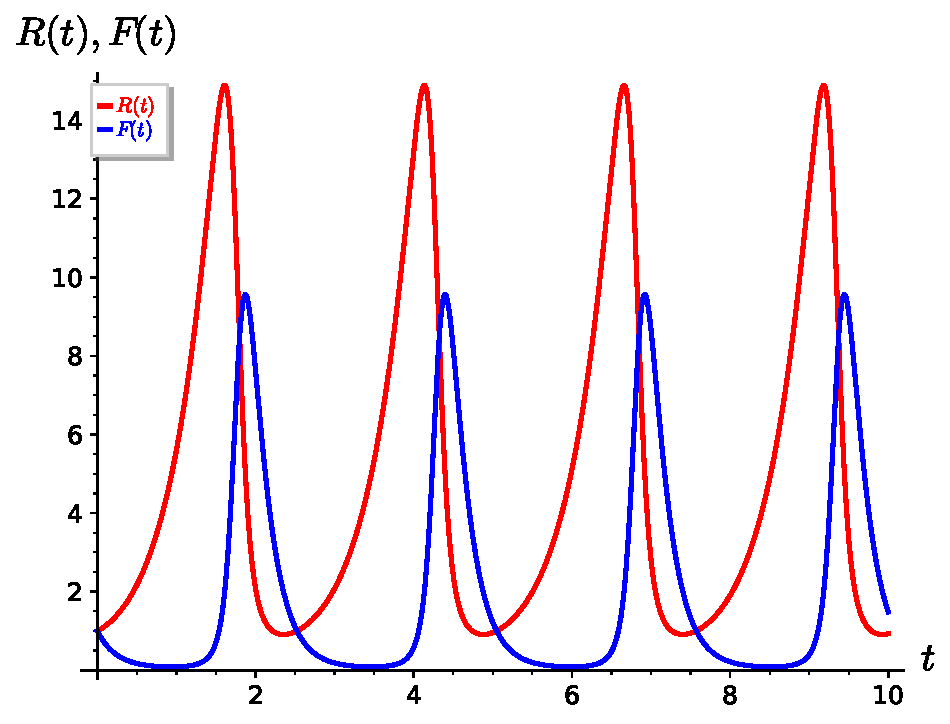
\includegraphics[width=\linewidth]{generated/sageplot/systems01-simple-predator-prey-system.pdf}%
\end{image}%
\tcblower
\end{figureptx}%
We can graph the solution to our system in a different manner\textemdash{}we can construct a parametric plot of our solution in the \(RF\)-plane. Thus, a point on the graph is given by \((R(t), F(t))\) at time \(t\). We can view the solution curve of our system in the \(RF\)-plane in \hyperref[x:figure:systems01-figure-solution-curve-predator-prey]{Figure~{\xreffont\ref{x:figure:systems01-figure-solution-curve-predator-prey}}}. The \(RF\)-plane is called the \terminology{phase plane}\index{phase plane} for our system of differential equations and is analogous to the phase line that we used during our investigation of slope fields for autonomous differential equations. We can plot many solutions to our predator-prey system and even plot direction fields in the phase plane (\hyperref[x:figure:systems01-figure-phase-plane-predator-prey]{Figure~{\xreffont\ref{x:figure:systems01-figure-phase-plane-predator-prey}}}).%
\begin{figureptx}{A solution curve in the \(RF\)-plane}{x:figure:systems01-figure-solution-curve-predator-prey}{}%
\begin{image}{0.2}{0.6}{0.2}%
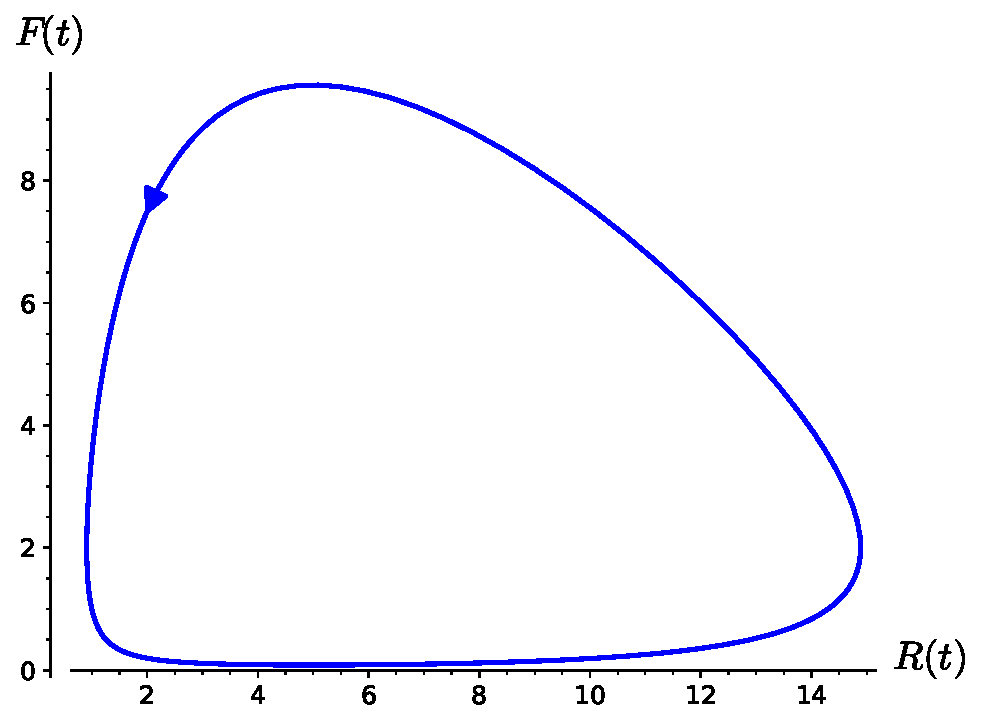
\includegraphics[width=\linewidth]{generated/sageplot/systems01-solution-curve-predator-prey.pdf}%
\end{image}%
\tcblower
\end{figureptx}%
\begin{figureptx}{The phase plane for a predator-prey system}{x:figure:systems01-figure-phase-plane-predator-prey}{}%
\begin{image}{0.2}{0.6}{0.2}%
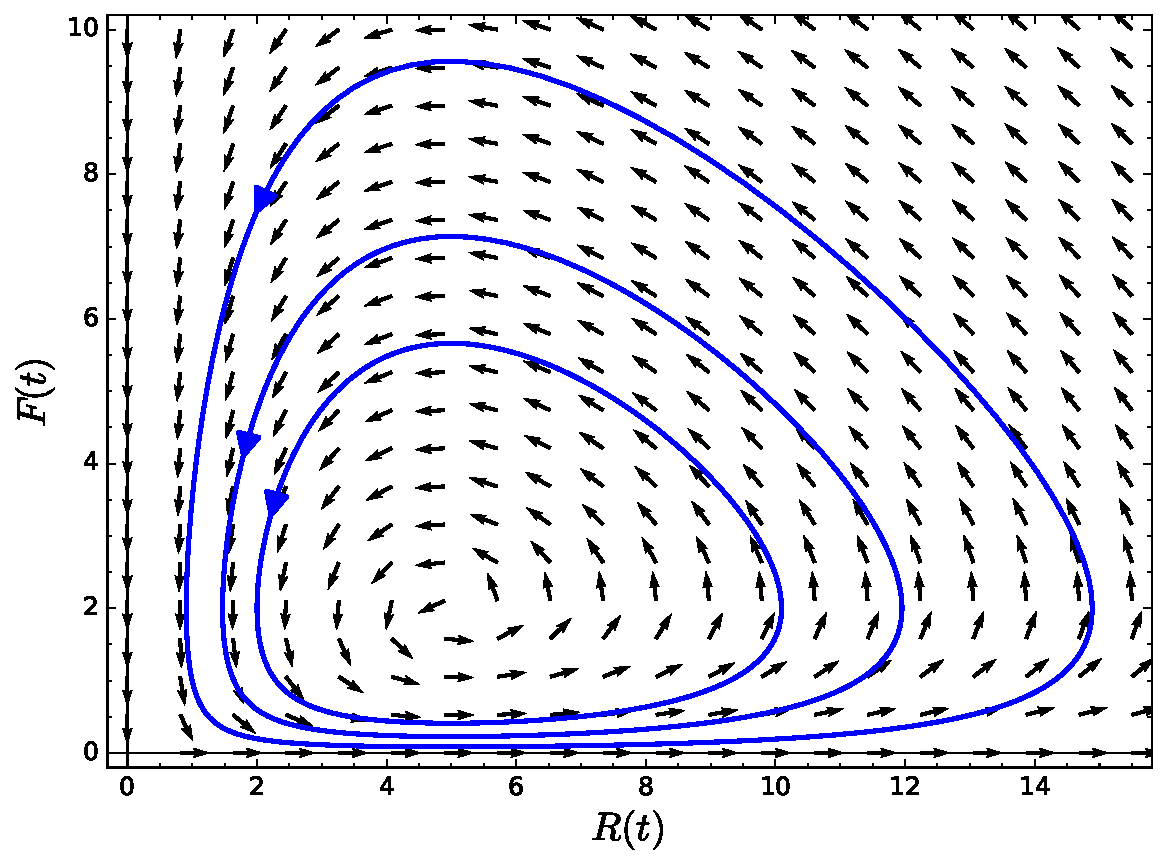
\includegraphics[width=\linewidth]{generated/sageplot/systems01-phase-plane-predator-prey.pdf}%
\end{image}%
\tcblower
\end{figureptx}%
We will now modify our system by assuming that the rabbit population will grow logistically if there are no predators present. The system can now be written as%
\begin{align*}
\frac{dR}{dt} & = aR(1 - R/N) - bRF,\\
\frac{dF}{dt} & = -cF + dRF,
\end{align*}
where \(N\) is the carrying capacity. As a specific example, consider the system%
\begin{align*}
\frac{dR}{dt} & = 2R\left(1 - \frac{R}{10}\right) - RF,\\
\frac{dF}{dt} & = -5F + RF.
\end{align*}
%
\par
It is easy to see that we have two equilibrium solutions\textemdash{}one at \((R, F) = (0, 0)\) and one at \((R, F) = (5, 1)\). Our solutions now behave very differently from the assumption that the population of the prey grows exponentially. If we have initial values \(R_0 = 1\) and \(F_0 = 1\), then our solution is no longer periodic (\hyperref[x:figure:systems01-figure-modified-predator-prey]{Figure~{\xreffont\ref{x:figure:systems01-figure-modified-predator-prey}}}). In fact, the solutions tend towards the equilibrium solution. The phase plane for our modified predator-prey system is given in \hyperref[x:figure:systems01-figure-modified-predator-prey-phase-plane]{Figure~{\xreffont\ref{x:figure:systems01-figure-modified-predator-prey-phase-plane}}}. The equilibrium solution \((5, 1)\) is an example of a \terminology{stable equilibrium solution}\index{equilibrium solution!stable}.%
\begin{figureptx}{Solutions for a modified predator-prey system}{x:figure:systems01-figure-modified-predator-prey}{}%
\begin{image}{0.2}{0.6}{0.2}%
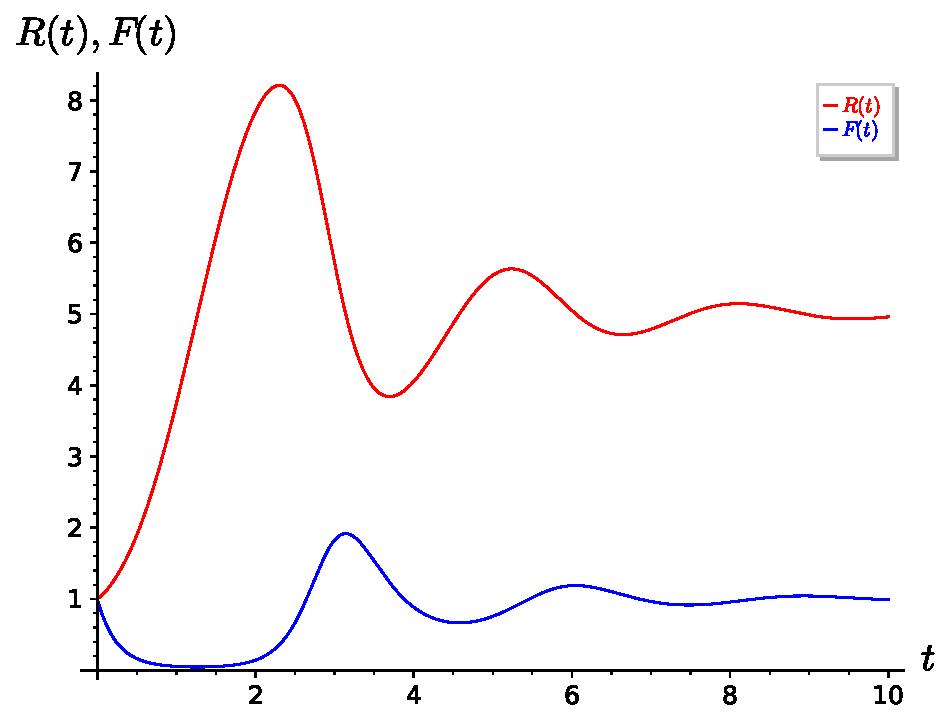
\includegraphics[width=\linewidth]{generated/sageplot/systems01-modified-predator-prey.pdf}%
\end{image}%
\tcblower
\end{figureptx}%
\begin{figureptx}{Phase plane for a modified predator-prey system}{x:figure:systems01-figure-modified-predator-prey-phase-plane}{}%
\begin{image}{0.2}{0.6}{0.2}%
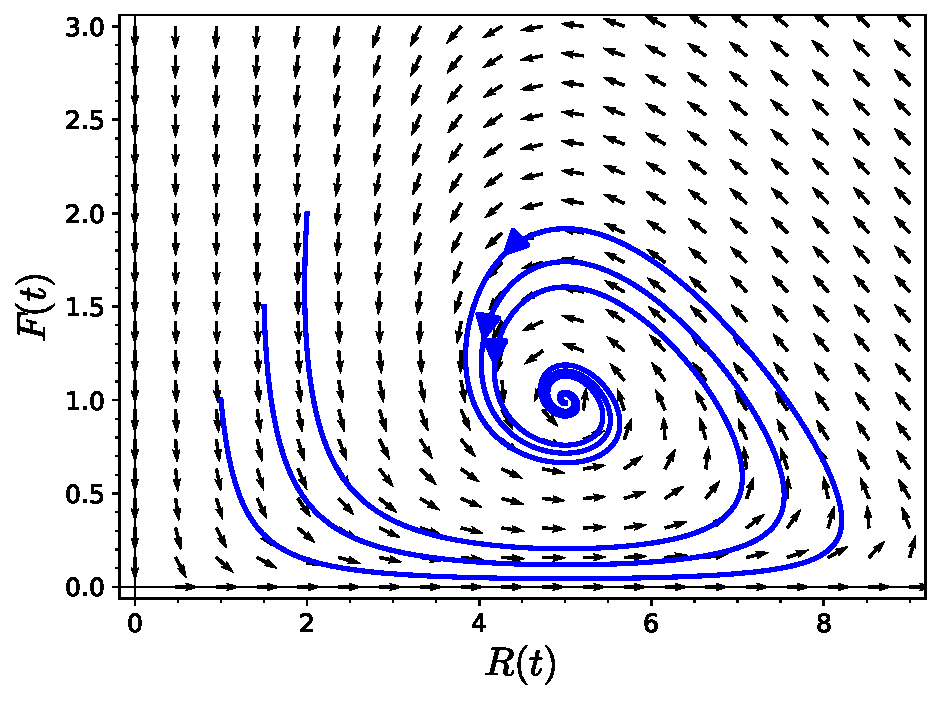
\includegraphics[width=\linewidth]{generated/sageplot/systems01-modified-predator-prey-phase-plane.pdf}%
\end{image}%
\tcblower
\end{figureptx}%
\begin{activity}{Modifying Predator-Prey Systems.}{g:activity:idp105545992986768}%
Consider the following predator-prey system,%
\begin{align*}
x' & = ax(1 - x/N) - bxy\\
y' & = -cy + dxy,
\end{align*}
where \(x(t)\) is the population of the prey and \(y(t)\) is the population of the predator at time \(t\).%
\begin{enumerate}[font=\bfseries,label=(\alph*),ref=\alph*]
\item{}How would you modify this system to include the effect of hunting of the prey at a rate of \(\alpha\) units of prey per unit of time?%
\item{}How would you modify this system to include the effect of hunting of the predators at a rate proportional to the number of predators?%
\item{}Suppose the predators discover a second, unlimited source of food, but they still prefer to eat the primary prey when they can catch them.  How would you modify the system to include this assumption?%
\item{}Suppose the predators discover a second source of food that is limited in supply. How would you modify the system to include this assumption?%
\item{}Suppose that the predators migrate to a different area if there are more than three times as many prey as predators in that area (\(x > 3y\)) and they move back if there are fewer than three times as many prey as predators. How would you modify the system to take this into account?%
\item{}Suppose that prey move out of an area at a rate proportional to the number of predators in the area.  How would you modify the system to take this into account?%
\end{enumerate}
\end{activity}%
\end{subsectionptx}
%
%
\typeout{************************************************}
\typeout{Subsection 2.1.2 The Spring-Mass Model Revisited}
\typeout{************************************************}
%
\begin{subsectionptx}{The Spring-Mass Model Revisited}{}{The Spring-Mass Model Revisited}{}{}{x:subsection:systems01-subsection-spring-mass}
Recall the spring-mass model from \hyperref[x:section:firstlook01]{Section~{\xreffont\ref{x:section:firstlook01}}}. We have a mass lying on a flat surface that is attached to one end of a spring with the other end of the spring attached to a wall. The spring displacement is denoted by \(x\). If \(x \gt 0\), then the spring is stretched. If \(x \lt 0\), the spring is compressed. If \(x = 0\), then the spring is in a state of equilibrium (\hyperref[x:figure:firstlook01-figure-spring-mass]{Figure~{\xreffont\ref{x:figure:firstlook01-figure-spring-mass}}}). If the surface is frictionless and we pull on the mass, then the mass will oscillate.%
\par
If we use a dashpot to add damping, the second-order differential equation for the spring-mass system is%
\begin{equation*}
mx'' = -bx' - kx.
\end{equation*}
or%
\begin{equation*}
mx'' + bx' + kx = 0,
\end{equation*}
where \(m\), \(b\), and \(k\) are all positive constants.%
\par
A second-order differential equation can be restated in terms of a system of first order differential equations. Given the differential equation%
\begin{equation*}
mx'' + bx' + kx = F(t),
\end{equation*}
with initial position \(x(0) = x_0\) and initial velocity \(x'(0) = x_0'\), we can rewrite this equation as a system of first-order differential equations by letting \(v(t) = x'(t)\). In this case, the equation becomes%
\begin{equation*}
mv' + bv + kx = F(t).
\end{equation*}
We now have a system of first-order differential equations,%
\begin{align*}
x' & = v,\\
v' & = \frac{1}{m} F(t) -\frac{b}{m} v -\frac{k}{m} x,
\end{align*}
with initial conditions%
\begin{align*}
x(0) & = x_0\\
v(0) & = v_0.
\end{align*}
%
\begin{activity}{A Harmonic Oscillator.}{g:activity:idp105545992969872}%
Consider the equation%
\begin{equation*}
\frac{d^2 y}{dt^2} + \frac{k}{m} y = 0
\end{equation*}
for the motion of a simple harmonic oscillator.%
\begin{enumerate}[font=\bfseries,label=(\alph*),ref=\alph*]
\item{}Rewrite the second-order differential equation, \(d^2 y/dt^2 + (k/m) y = 0\), as a system of two first-order differentail equations, where \(v = y'\).%
\item{}Consider the function \(y(t) = \cos \beta t\). Under what conditions on \(\beta\) is \(y(t)\) a solution to the differential equation?%
\item{}What initial condition (\(t = 0\)) in the \(yv\)-plane corresponds to this solution?%
\item{}In terms of \(k\) and \(m\), what is the period of this solution?%
\item{}Sketch the solution curve in the \(yv\)-plane that corresponds to this solution.%
\end{enumerate}
\end{activity}%
\end{subsectionptx}
%
%
\typeout{************************************************}
\typeout{Subsection 2.1.3 Modeling Epidemics}
\typeout{************************************************}
%
\begin{subsectionptx}{Modeling Epidemics}{}{Modeling Epidemics}{}{}{x:subsection:systems01-subsection-epidemics}
Systems of differential equations are very useful in epidemiology. Differential equations can be used to model various epidemics, including the  bubonic plague, influenza, AIDS, the 2015 ebola outbreak in west Africa, and the COVID-19 pandemic. To understand how we might model an epidemic, we will consider a very simple situation. We will assume that we have a closed population of size \(N\), where immigration, emigration, and birth do not play an important role. We will also ignore any deaths that are not related to our disease.%
\par
We will assume that each individual in the population falls into one of the following categories:%
\begin{align*}
s(t) & = \text{Susceptible individuals}\\
i(t) & = \text{Infected individuals}\\
r(t) & = \text{Removed individuals}
\end{align*}
Susceptible individuals are those who do not yet have the disease and can catch the disease from infected individuals. Individuals enter the removed population by either recovering from the disease or dying. If an infected individual recovers, then the individual is immune to the disease. Schematically, we can represent the effect of the disease by the diagram%
\begin{equation*}
s \longrightarrow i \longrightarrow r.
\end{equation*}
Since the population is closed, we know that%
\begin{equation*}
s(t) + i(t) + r(t) = N.
\end{equation*}
This model is called an \terminology{SIR model}\index{SIR model}.%
\par
We can model how the disease acts with the following system of equations,%
\begin{align*}
\frac{ds}{dt} & = - \alpha si\\
\frac{di}{dt} & = \alpha si - \beta i\\
\frac{dr}{dt} & = \beta i.
\end{align*}
We say that \(\alpha\) is the rate of infection and \(\beta\) is the rate at which the infected are removed. That is, an infected individual either dies or recovers after \(1/ \beta\) days. Since%
\begin{equation*}
\frac{d}{dt}\left[ s(t) + i(t) + r(t)\right] = \frac{d}{dt} N = 0,
\end{equation*}
we need only solve the system%
\begin{align*}
\frac{ds}{dt} & = - \alpha si\\
\frac{di}{dt} & = \alpha si - \beta i.
\end{align*}
Letting \(\alpha = 0.005\) and \(\beta = 0.08\), we can see how the susceptible and infected populations interact in an SIR epidemic in \hyperref[x:figure:systems01-figure-SIR-epidemic]{Figure~{\xreffont\ref{x:figure:systems01-figure-SIR-epidemic}}}.%
\begin{figureptx}{The susceptible and removed populations for an SIR epidemic}{x:figure:systems01-figure-SIR-epidemic}{}%
\begin{image}{0.2}{0.6}{0.2}%
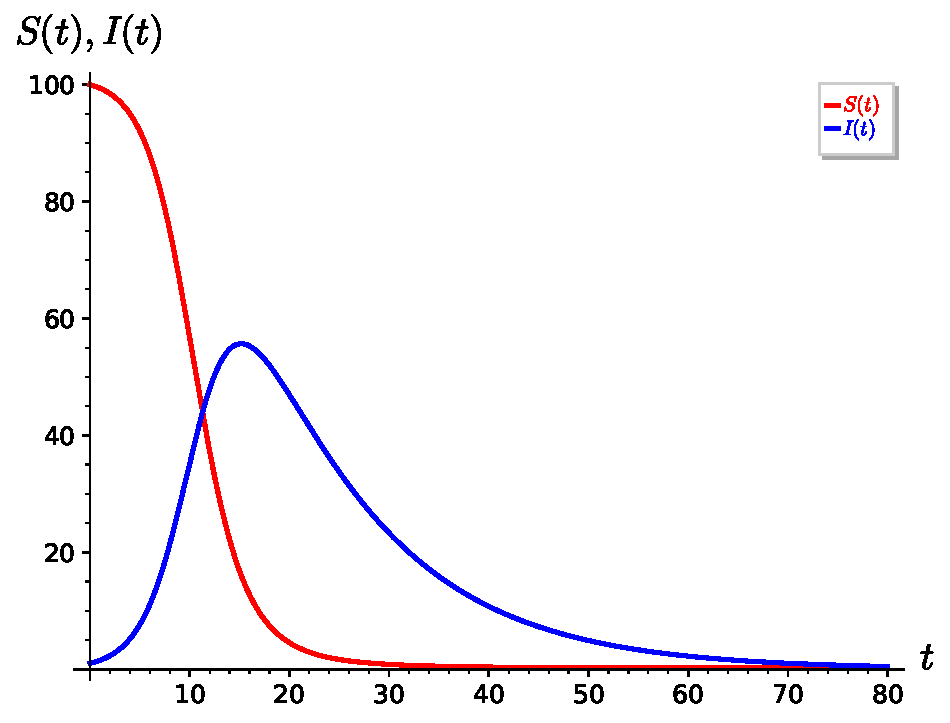
\includegraphics[width=\linewidth]{generated/sageplot/systems01-SIR-epidemic.pdf}%
\end{image}%
\tcblower
\end{figureptx}%
There are many questions associated with epidemic models.%
\begin{itemize}[label=\textbullet]
\item{}Will there be an epidemic?%
\item{}If there is an epidemic, how many individuals will be infected?%
\item{}Is there a period of time for which individuals are exposed to the disease but exhibit no symptoms and cannot infect others?%
\item{}If the disease is endemic, what is the prevalence of the infection?%
\item{}Can the disease be eradicated or controlled?%
\item{}What is the effect of the population age structure?%
\end{itemize}
To explore \(SIR\) models in more depth, see \hyperref[x:project:systems05-project-epidemiology]{Project~{\xreffont\ref{x:project:systems05-project-epidemiology}}}.%
\end{subsectionptx}
%
%
\typeout{************************************************}
\typeout{Subsection 2.1.4 Important Lessons}
\typeout{************************************************}
%
\begin{subsectionptx}{Important Lessons}{}{Important Lessons}{}{}{x:subsection:systems01-subsection-important-lessons}
%
\begin{itemize}[label=\textbullet]
\item{}A \terminology{second-order linear equation}%
\begin{equation*}
a(t) x'' + b(t) x' + c(t) x = g(t)
\end{equation*}
can be written as a system of first-order equations by letting \(v(t) = x'(t)\).%
\item{}We define an \terminology{equilibrium solution} for a system of differential equations%
\begin{align*}
\frac{dx}{dt} & = f(x, y)\\
\frac{dy}{dt} & = g(x, y)
\end{align*}
to be those values of \(x\) and \(y\) such that \(f(x, y) = 0\) and \(g(x, y) = 0\).%
\item{}We can graph solutions to the system%
\begin{align*}
\frac{dx}{dt} & = f(x, y),\\
\frac{dy}{dt} & = g(x, y),
\end{align*}
as parametric plots in the \(xy\)-plane.  A point on the graph is given by \((x(t), y(t))\) at time \(t\). The \(xy\)-plane is called the \terminology{phase plane} for our system of differential equations.%
\item{}Solution curves in the phase plane of%
\begin{align*}
\frac{dx}{dt} & = f(x, y),\\
\frac{dy}{dt} & = g(x, y),
\end{align*}
can act very differently depending on how close they are to a particular equilibrium solution.%
\end{itemize}
%
\end{subsectionptx}
%
%
\typeout{************************************************}
\typeout{Reading Questions 2.1.5 Reading Questions}
\typeout{************************************************}
%
\begin{reading-questions-subsection}{Reading Questions}{}{Reading Questions}{}{}{x:reading-questions:reading-questions-system01}
\begin{divisionexercise}{1}{}{}{x:exercise:reading-questions-system01-2}%
Given a system of first-order differential equations, explain in your own words what it means to be a stable equilibrium solution for the system.%
\end{divisionexercise}%
\end{reading-questions-subsection}
%
%
\typeout{************************************************}
\typeout{Exercises 2.1.6 Exercises}
\typeout{************************************************}
%
\begin{exercises-subsection}{Exercises}{}{Exercises}{}{}{x:exercises:systems01-exercises}
\begin{divisionexercise}{1}{}{}{g:exercise:idp105545992740752}%
Verify whether or not the given pair of functions, \((x(t), y(t))\) forms a solution to the system%
\begin{align*}
\frac{dx}{dt} & = 4x + 2y\\
\frac{dy}{dt} & = 3x - y
\end{align*}
%
\begin{enumerate}[label=(\alph*)]
\item{}\(x(t) = e^{-2t} + 2e^{5t}\), \(y(t) = -3e^{-2t} + e^{5t}\)%
\item{}\(x(t) = 2e^{-2t} \), \(y(t) = -6 e^{-2t} \)%
\item{}\(x(t) = 2e^{-2t} \), \(y(t) = -5 e^{-2t} \)%
\item{}\(x(t) = c_1e^{-2t} + 2c_2e^{5t}\), \(y(t) = -3c_1 e^{-2t} + c_2 e^{5t}\)%
\end{enumerate}
%
\end{divisionexercise}%
\begin{divisionexercise}{2}{}{}{g:exercise:idp105545992746128}%
Verify whether or not the given pair of functions, \((x(t), y(t))\) forms a solution to the system%
\begin{align*}
\frac{dx}{dt} & = 4x -3y\\
\frac{dy}{dt} & = 3x + 4y
\end{align*}
%
\begin{enumerate}[label=(\alph*)]
\item{}\(x(t) = 2e^{4t}\cos 3t\), \(y(t) = 2e^{4t}\sin 3t\)%
\item{}\(x(t) = 2e^{4t}\cos 3t - 3e^{4t}\sin 3t\), \(y(t) = 2e^{4t}\sin 3t + 3e^{4t}\cos 3t\)%
\item{}\(x(t) = 3e^{4t}\cos 3t - 4e^{4t}\sin 3t\), \(y(t) = 3e^{4t}\sin 3t + 5e^{4t}\cos 3t\)%
\item{}\(x(t) =c_1e^{4t}\cos 3t - c_2e^{4t}\sin 3t\), \(y(t) = c_1e^{4t}\sin 3t + c_2e^{4t}\cos 3t\)%
\end{enumerate}
%
\end{divisionexercise}%
\begin{divisionexercise}{3}{}{}{g:exercise:idp105545992751504}%
A system is \terminology{autonomous}\index{system!autonomous} if \(dx/dt\) and \(dx/dt\) dop not depend on \(t\); that is,%
\begin{align*}
\frac{dx}{dt} & = f(x,y)\\
\frac{dy}{dt} & = g(x,y).
\end{align*}
Which of the following systems are autonomous?%
\begin{enumerate}[label=(\alph*)]
\item{}%
\begin{align*}
\frac{dx}{dt} & = 4x -3y\\
\frac{dy}{dt} & = 3x + 4y
\end{align*}
%
\item{}%
\begin{align*}
\frac{dx}{dt} & = 4x -3y + \cos x\\
\frac{dy}{dt} & = 3x + 4y - \sin x
\end{align*}
%
\item{}%
\begin{align*}
\frac{dx}{dt} & = 4x -3y +3tx\\
\frac{dy}{dt} & = 3x + 4y - e^x
\end{align*}
%
\item{}%
\begin{align*}
\frac{dx}{dt} & = 4x \\
\frac{dy}{dt} & =  4y
\end{align*}
%
\end{enumerate}
%
\end{divisionexercise}%
\begin{divisionexercise}{4}{}{}{g:exercise:idp105545992791440}%
Change each of the following second-order initial value problems into a system of equations.%
\begin{enumerate}[label=(\alph*)]
\item{}%
\begin{align*}
x'' + 6x' - 2x \amp = 0\\
x(0) \amp = 1\\
x'(0) \amp = 1
\end{align*}
%
\item{}%
\begin{align*}
y'' + y' - 2y \amp = 0\\
y(0) \amp = 2\\
y'(0) \amp = 0
\end{align*}
%
\item{}%
\begin{align*}
\frac{d^2x}{dt^2} + \frac{dx}{dt}' + 4x \amp = \sin t\\
x(0) \amp = 4\\
x'(0) \amp = -3
\end{align*}
%
\item{}%
\begin{align*}
x'' + tx' - 2 \amp = 0\\
x(0) \amp = 0\\
x'(0) \amp = 1
\end{align*}
%
\end{enumerate}
%
\end{divisionexercise}%
\begin{divisionexercise}{5}{}{}{g:exercise:idp105545992796688}%
Change each of the following second-order initial value problems into a system of equations.%
\begin{enumerate}[label=(\alph*)]
\item{}%
\begin{align*}
x'' + 6x' - 2x \amp = 0\\
x(0) \amp = 1\\
x'(0) \amp = 1
\end{align*}
%
\item{}%
\begin{align*}
y'' + y' - 2y \amp = 0\\
y(0) \amp = 2\\
y'(0) \amp = 0
\end{align*}
%
\item{}%
\begin{align*}
\frac{d^2x}{dt^2} + \frac{dx}{dt}' + 4x \amp = \sin t\\
x(0) \amp = 4\\
x'(0) \amp = -3
\end{align*}
%
\item{}%
\begin{align*}
x'' + tx' - 2 \amp = 0\\
x(0) \amp = 0\\
x'(0) \amp = 1
\end{align*}
%
\end{enumerate}
%
\end{divisionexercise}%
\begin{divisionexercise}{6}{}{}{g:exercise:idp105545992801936}%
Consider the SIR model%
\begin{align*}
\frac{dS}{dt} & = - \alpha SI\\
\frac{dI}{dt} & = \alpha SI - \beta I,
\end{align*}
where \(S\) is the susceptible population and \(I\) is the infected population.%
\begin{enumerate}[label=(\alph*)]
\item{}Modify the SIR model to account for the situation where the susceptible population is reproducing at a rate proportional to the current population.%
\item{}Modify the SIR model to account for the situation where the susceptible population is decreasing at a constant rate such as susceptibles leaving an infected area or city.%
\item{}Modify the SIR model to account for the situation where the infected population is increasing at a constant rate such as infected individuals entering an infected area or city from the outside.%
\end{enumerate}
%
\end{divisionexercise}%
\begin{divisionexercise}{7}{}{}{g:exercise:idp105545992772496}%
A mass weighing 4 pounds stretches a spring 4 inches.%
\begin{enumerate}[label=(\alph*)]
\item{}Consider the function \(y(t) = \cos \beta t\). Under what conditions on \(\beta\) is \(y(t)\) a solution to the differential equation?%
\item{}Formulate an initial value problem that corresponds to the motion of this undamped mass-spring system if the mass is extended \(1\) foot from its rest position and released with no initial velocity.%
\item{}Using the result of the previous exercise, find the solution of this initial value problem.%
\end{enumerate}
%
\end{divisionexercise}%
\end{exercises-subsection}
%
%
\typeout{************************************************}
\typeout{Subsection 2.1.7 Using \emph{Sage} to Solve Systems}
\typeout{************************************************}
%
\begin{subsectionptx}{Using \emph{Sage} to Solve Systems}{}{Using \emph{Sage} to Solve Systems}{}{}{x:subsection:systems01-subsection-sage}
We can use \emph{Sage} to plot the solution of the system%
\begin{align}
x' & = -x - y\label{x:mrow:systems01-equation-desolve-rk4-system-1}\\
y' & = x + y/5\label{x:mrow:systems01-equation-desolve-rk4-system-2}\\
x(0) & = 1\label{x:mrow:systems01-equation-desolve-rk4-system-3}\\
y(0) & = -1\label{x:mrow:systems01-equation-desolve-rk4-system-4}
\end{align}
First, let us plot a direction field for our system.%
\begin{sageinput}
x, y, t = var('x y t')
F = [-x - y, x + y/5]
p = plot_vector_field(F, (x,-4,4), (y,-4,4))
p
\end{sageinput}
\begin{sageoutput}

\end{sageoutput}
Notice the vectors are different lengths depending on their magnitudes. If we wish all of the vectors to be the same length, we can divide each component by the length of the vector.%
\begin{sageinput}
x, y, t = var('x y t')
F = [-x - y, x + y/5]
n = sqrt(F[0]^2 + F[1]^2)
F_unit = [F[0]/n, F[1]/n]
p = plot_vector_field(F_unit, (x,-4,4), (y,-4,4))
p
\end{sageinput}
\begin{sageoutput}

\end{sageoutput}
We can also add axes labels to our plot.%
\begin{sageinput}
x, y, t = var('x y t')
F = [-x - y, x + y/5]
n = sqrt(F[0]^2 + F[1]^2)
F_unit = [F[0]/n, F[1]/n]
p = plot_vector_field(F_unit, (x,-4,4), (y,-4,4), axes_labels=['$x(t)$','$y(t)$'])
p
\end{sageinput}
\begin{sageoutput}

\end{sageoutput}
Now suppose that we wish to plot solutions \(x(t)\) and \(y(t)\) to our system. We can use the \emph{Sage} command \mono{desolve\_system\_rk4}.%
\begin{sageinput}
x, y, t = var('x y t')
F = [-x - y, x + y/5]
P = desolve_system_rk4(F, [x, y], ics = [0,1,-1], ivar = t, end_points = 10, step = 0.01)
P
\end{sageinput}
\begin{sageoutput}

\end{sageoutput}
We now have a numerical approximation of the solution to the system \hyperref[x:mrow:systems01-equation-desolve-rk4-system-1]{({\xreffont\ref{x:mrow:systems01-equation-desolve-rk4-system-1}})}\textendash{}\hyperref[x:mrow:systems01-equation-desolve-rk4-system-4]{({\xreffont\ref{x:mrow:systems01-equation-desolve-rk4-system-4}})}. However, our approximation is just a very long list of points. In fact, we get a list of triples, \((t, x, y)\). It would be much more useful if we could display a graph of the solution. In the code below, we grab pairs \((t,x)\) and \((t, y)\) and then plot the points using the \mono{line} command.%
\begin{sageinput}
x, y, t = var('x y t')
F = [-x - y, x + y/5]
P = desolve_system_rk4(F, [x, y], ics = [0,1,-1], ivar = t, end_points = 10, step = 0.01)
Q = [ [i, j] for i,j,k in P]
R = [ [i, k] for i,j,k in P]
p = line(Q)
p += line(R)
p
\end{sageinput}
\begin{sageoutput}

\end{sageoutput}
We can also add colors, axes labels, and legend colors so that the plot makes more sense.%
\begin{sageinput}
x, y, t = var('x y t')
F = [-x - y, x + y/5]
P = desolve_system_rk4(F, [x, y], ics = [0,1,-1], ivar = t, end_points = 10, step = 0.01)
Q = [ [i, j] for i,j,k in P]
R = [ [i, k] for i,j,k in P]
p = line(Q, color='red', axes_labels=['$t$','$x(t), y(t)$'], legend_label='$x(t)$', legend_color='red', fontsize=12)
p += line(R, color='blue', legend_label='$y(t)$', legend_color='blue')
p
\end{sageinput}
\begin{sageoutput}

\end{sageoutput}
To plot the solution in the \(xy\)\textendash{}plane, we will need to select the second two entries in each triple.%
\begin{sageinput}
x, y, t = var('x y t')
F = [-x - y, x + y/5]
P = desolve_system_rk4(F, [x, y], ics = [0,1,-1], ivar = t, end_points = 10, step = 0.01)
Q = [ [j,k] for i,j,k in P]
p = line(Q, axes_labels=['$x(t)$','$y(t)$'], fontsize=12)
p
\end{sageinput}
\begin{sageoutput}

\end{sageoutput}
We can adjust the thickness of the plot add an arrow to indicate the direction of the solution.%
\begin{sageinput}
x, y, t = var('x y t')
F = [-x - y, x + y/5]
P = desolve_system_rk4(F, [x, y], ics = [0,1,-1], ivar = t, end_points = 10, step = 0.01)
Q = [ [j,k] for i,j,k in P]
p = line(Q, axes_labels=['$x(t)$','$y(t)$'], fontsize=12, thickness=3)
p += arrow(Q[int(len(Q)/5)], Q[int(len(Q)/5) + 1])
p
\end{sageinput}
\begin{sageoutput}

\end{sageoutput}
Now let us add a vector field to our plot.%
\begin{sageinput}
x, y, t = var('x y t')
F = [-x - y, x + y/5]
P = desolve_system_rk4(F, [x, y], ics = [0,1,-1], ivar = t, end_points = 10, step = 0.01)
Q = [ [j,k] for i,j,k in P]
p = line(Q, axes_labels=['$x(t)$','$y(t)$'], fontsize=12, thickness=3)
p += arrow(Q[int(len(Q)/5)], Q[int(len(Q)/5) + 1])
n = sqrt(F[0]^2 + F[1]^2)
F_unit = [F[0]/n, F[1]/n]
p += plot_vector_field(F_unit, (x,-1.5,1.5), (y,-1.5,1.5), axes_labels=['$x(t)$','$y(t)$'])
p
\end{sageinput}
\begin{sageoutput}

\end{sageoutput}
To learn more about how to use Sage to solve systems of differential equations, see \href{http://www.sagemath.org/doc/reference/calculus/sage/calculus/desolvers.html}{\nolinkurl{www.sagemath.org/doc/reference/calculus/sage/calculus/desolvers.html}}. The Sage cell below can be used to make your own computations.%
\begin{sageinput}

\end{sageinput}
\begin{sageoutput}

\end{sageoutput}
\end{subsectionptx}
\end{sectionptx}
%
%
\typeout{************************************************}
\typeout{Section 2.2 The Geometry of Systems}
\typeout{************************************************}
%
\begin{sectionptx}{The Geometry of Systems}{}{The Geometry of Systems}{}{}{x:section:systems02}
\begin{objectives}{Objectives}{g:objectives:idp105545992827792}
%
\begin{itemize}[label=\textbullet]
\item{}To understand how the righthand side of the system%
\begin{align*}
\frac{dx}{dt} & = f(x, y)\\
\frac{dy}{dt} & = g(x, y)
\end{align*}
can be viewed as a vector field, \((f(x,y), g(x,y))\), which can be plotted in the \(x,y\)-plane.%
\item{}To understand and be able to use nullclines and phase plane analysis to sketch solution curves for the system%
\begin{align*}
\frac{dx}{dt} & = f(x, y)\\
\frac{dy}{dt} & = g(x, y).
\end{align*}
%
\end{itemize}
\end{objectives}
\begin{introduction}{}%
We can use \terminology{direction fields}\index{system!direction field} in the phase plane to represent \terminology{autonomous systems}\index{system!autonomous}%
\begin{align}
\frac{dx}{dt} & = f(x, y),\label{x:mrow:systems02-equation-harmonic-oscillator-1}\\
\frac{dy}{dt} & = g(x, y).\label{x:mrow:systems02-equation-harmonic-oscillator-2}
\end{align}
Equation~\hyperref[x:mrow:systems02-equation-harmonic-oscillator-1]{({\xreffont\ref{x:mrow:systems02-equation-harmonic-oscillator-1}})} tells us how a solution curve changes in the \(x\) direction, while equation~\hyperref[x:mrow:systems02-equation-harmonic-oscillator-2]{({\xreffont\ref{x:mrow:systems02-equation-harmonic-oscillator-2}})} tells us how a solution curve changes in the \(y\) direction.%
\end{introduction}%
%
%
\typeout{************************************************}
\typeout{Subsection 2.2.1 Direction Fields}
\typeout{************************************************}
%
\begin{subsectionptx}{Direction Fields}{}{Direction Fields}{}{}{x:subsection:systems02-subsection-direction-fields}
\begin{example}{}{g:example:idp105545992804496}%
Consider the differential equation for a simple harmonic oscillator that we developed in \hyperref[x:section:firstlook01]{Section~{\xreffont\ref{x:section:firstlook01}}},%
\begin{equation*}
mx'' + kx = 0.
\end{equation*}
If we assume that \(k\) and \(m\) are both equal to one and let \(x' = v\), we can rewrite this equation as the first order system,%
\begin{align*}
x' & = v,\\
v' & = -x.
\end{align*}
The direction field is relatively easy to understand. After plotting only few vectors, we can very quickly see that the vectors are tangent to circles centered at the origin (\hyperref[x:figure:systems02-figure-harmonic-oscillator]{Figure~{\xreffont\ref{x:figure:systems02-figure-harmonic-oscillator}}}). Since the solutions to the undamped harmonic oscillator \(x'' + x = 0\) are of the form%
\begin{equation*}
x(t) =  A \cos t + B \sin t
\end{equation*}
for arbitrary constants \(A\) and \(B\), this should not be too surprising.%
\begin{figureptx}{The direction field for a harmonic oscillator}{x:figure:systems02-figure-harmonic-oscillator}{}%
\begin{image}{0.2}{0.6}{0.2}%
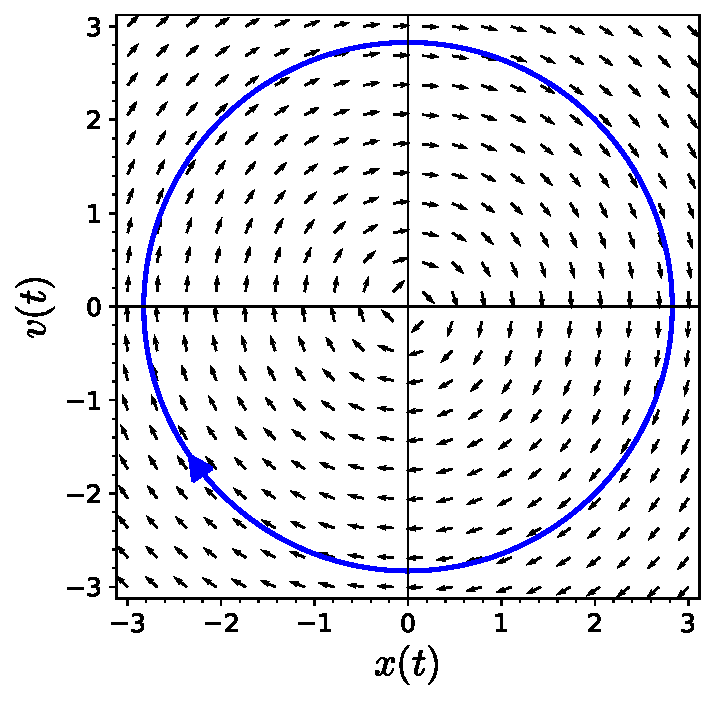
\includegraphics[width=\linewidth]{generated/sageplot/systems02-harmonic-oscillator.pdf}%
\end{image}%
\tcblower
\end{figureptx}%
\end{example}
Let us examine some systems of equations with direction fields that are easily plotted.%
\begin{example}{}{g:example:idp105545992811152}%
The system%
\begin{align*}
x' & = x\\
y' & = y
\end{align*}
gives us a direction field where the vectors point away from the origin (\hyperref[x:figure:systems02-figure-direction-field-example-1]{Figure~{\xreffont\ref{x:figure:systems02-figure-direction-field-example-1}}}).%
\begin{figureptx}{The direction field for \(x' = x\) and \(y' = y\)}{x:figure:systems02-figure-direction-field-example-1}{}%
\begin{image}{0.2}{0.6}{0.2}%
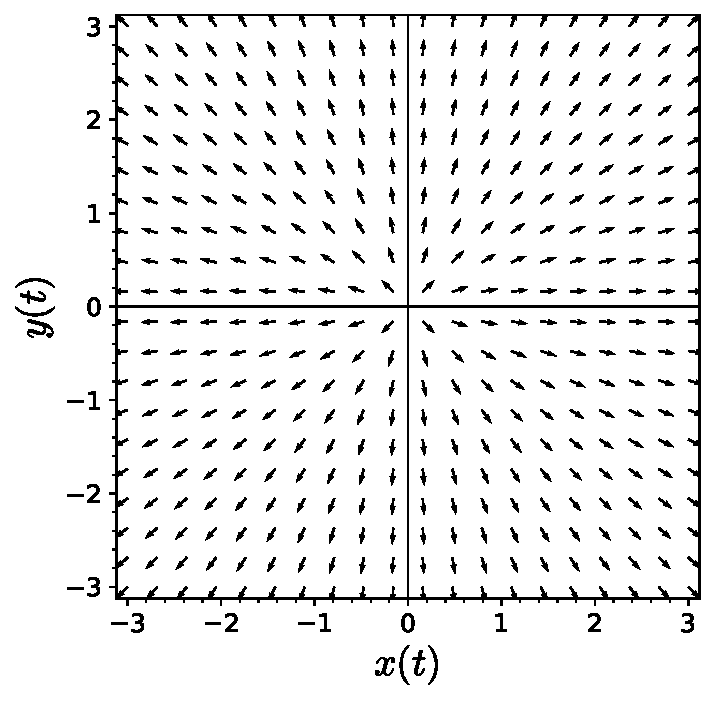
\includegraphics[width=\linewidth]{generated/sageplot/systems02-direction-field-example-1.pdf}%
\end{image}%
\tcblower
\end{figureptx}%
The system%
\begin{align*}
x' & = -x,\\
y' & = -y.
\end{align*}
gives us a direction field where the vectors point towards the origin (\hyperref[x:figure:systems02-figure-direction-field-example-2]{Figure~{\xreffont\ref{x:figure:systems02-figure-direction-field-example-2}}}).%
\begin{figureptx}{The direction field for \(x' = -x\) and \(y' = -y\)}{x:figure:systems02-figure-direction-field-example-2}{}%
\begin{image}{0.2}{0.6}{0.2}%
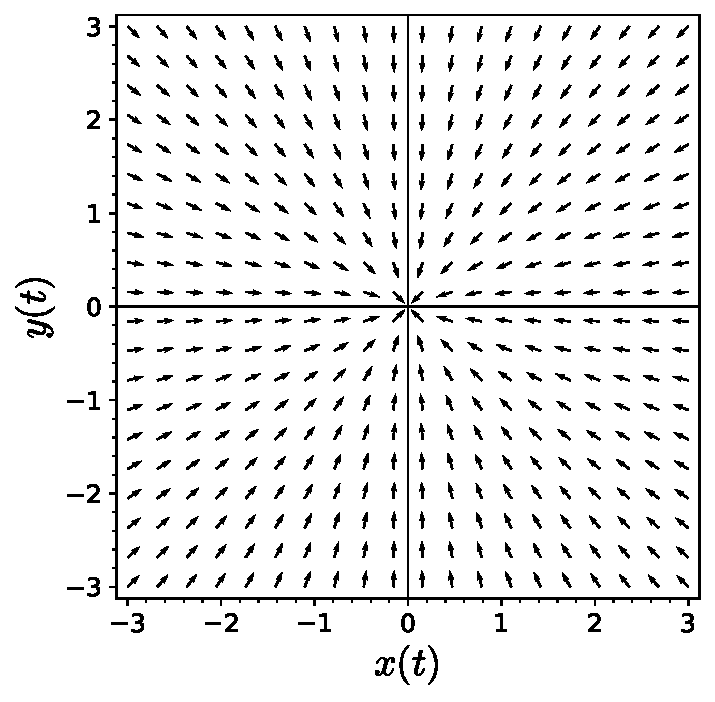
\includegraphics[width=\linewidth]{generated/sageplot/systems02-direction-field-example-2.pdf}%
\end{image}%
\tcblower
\end{figureptx}%
The system%
\begin{align*}
x' & = -x,\\
y' & = -5y.
\end{align*}
also gives us a direction field where the vectors point towards the origin; however, we shall soon see that there are important differences between this direction field and the direction field of the previous system (\hyperref[x:figure:systems02-figure-direction-field-example-2]{Figure~{\xreffont\ref{x:figure:systems02-figure-direction-field-example-2}}}).%
\begin{figureptx}{The direction field for \(x' = -x\) and \(y' = -5y\)}{x:figure:systems02-figure-direction-field-example-3}{}%
\begin{image}{0.2}{0.6}{0.2}%
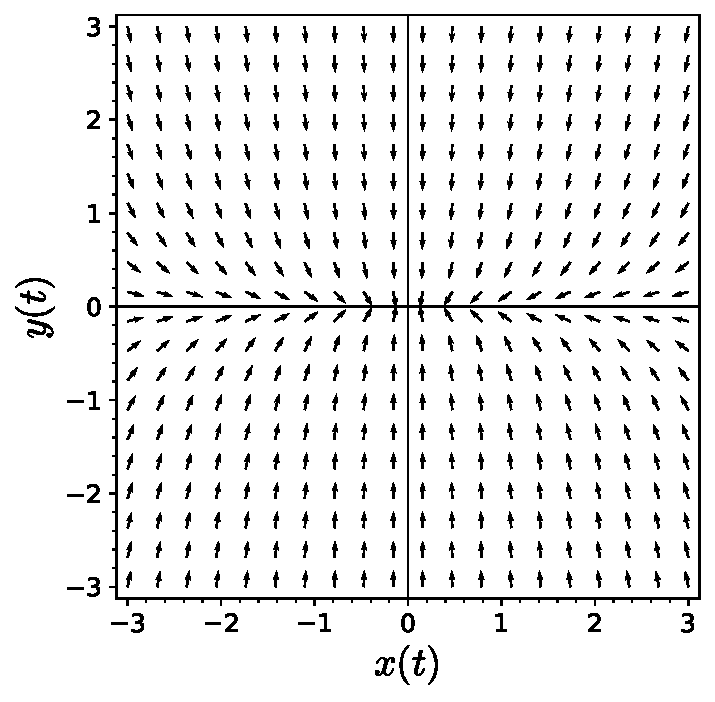
\includegraphics[width=\linewidth]{generated/sageplot/systems02-direction-field-example-3.pdf}%
\end{image}%
\tcblower
\end{figureptx}%
\end{example}
\begin{activity}{Plotting Direction Fields.}{g:activity:idp105545992854544}%
Plot direction fields for each of the following systems of differential equations in the \(xy\)-plane.%
\begin{enumerate}[font=\bfseries,label=(\alph*),ref=\alph*]
\item{}%
\begin{align*}
x' & = -3x\\
y' & = 4y
\end{align*}
%
\item{}%
\begin{align*}
x' & = 2x\\
y' & = y/2
\end{align*}
%
\item{}%
\begin{align*}
x' & = x/2\\
y' & = 2y
\end{align*}
%
\item{}%
\begin{align*}
x' & = x + y\\
y' & = x - y
\end{align*}
%
\end{enumerate}
\end{activity}%
\end{subsectionptx}
%
%
\typeout{************************************************}
\typeout{Subsection 2.2.2 Modified Predator-Prey System}
\typeout{************************************************}
%
\begin{subsectionptx}{Modified Predator-Prey System}{}{Modified Predator-Prey System}{}{}{x:subsection:systems02-subsection-predator-prey}
Let us recall the modified predator-prey system that we developed in the last section. That is, we will assume that the prey in our model has logistic growth,%
\begin{align*}
\frac{dR}{dt} & = aR(1 - R/N) - bRF,\\
\frac{dF}{dt} & = -cF + dRF,
\end{align*}
where \(N\) is the carrying capacity. In order to investigate the geometric properties of our system, we will rewrite our system in vector form.  For each value of \(t\), we will use \({\mathbf x}(t)\) to denote the vector-valued function%
\begin{equation*}
{\mathbf x}(t) = \begin{pmatrix} R(t) \\ F(t) \end{pmatrix}.
\end{equation*}
This vector-valued function, \(\mathbf x(t)\) corresponds to our solution curve \((R(t), F(t))\) in the \(RF\)-plane. Now we can write our predator-prey model as a single vector equation,%
\begin{equation*}
\frac{d \mathbf x}{dt} = \begin{pmatrix} R'(t) \\ F'(t) \end{pmatrix} = \begin{pmatrix} aR(1 - R/N) - bRF, \\ -cF + dRF \end{pmatrix}.
\end{equation*}
%
\par
We can view the right side of the equation as a \terminology{vector field}\index{vector field}. The specific example that we examined was%
\begin{align*}
\frac{dR}{dt} & = 2R\left(1 - \frac{R}{10}\right) - RF,\\
\frac{dF}{dt} & = -5F + RF.
\end{align*}
The vector field form of this system is%
\begin{equation*}
\frac{d \mathbf x}{dt} = \begin{pmatrix} 2R(1 - R/10) - RF \\ -5F + RF \end{pmatrix}.
\end{equation*}
We can associate a vector in the \(RF\)-plane for each value of \(R\) and \(F\). For example, if we let \((R, F) = (10, 10)\), we have \((R', F') = (-100, 50)\).  At this particular point, the population of rabbits is falling rapidly while the number of foxes is climbing very quickly, We can represent this vector in the phase plane by drawing an arrow in the proper direction. Thus, we obtain a direction field for our system of differential equations (\hyperref[x:figure:systems02-figure-predator-prey]{Figure~{\xreffont\ref{x:figure:systems02-figure-predator-prey}}}).%
\begin{figureptx}{A vector field for the predator-prey system}{x:figure:systems02-figure-predator-prey}{}%
\begin{image}{0.2}{0.6}{0.2}%
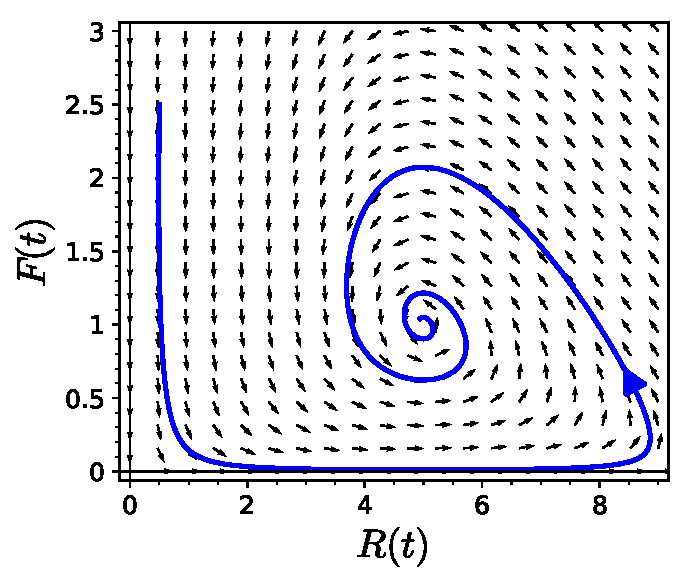
\includegraphics[width=\linewidth]{generated/sageplot/systems02-predator-prey.pdf}%
\end{image}%
\tcblower
\end{figureptx}%
\end{subsectionptx}
%
%
\typeout{************************************************}
\typeout{Subsection 2.2.3 A Competing Species Model}
\typeout{************************************************}
%
\begin{subsectionptx}{A Competing Species Model}{}{A Competing Species Model}{}{}{x:subsection:systems02-subsection-competing-species}
Suppose that \(x\) and \(y\) are the population of two distinct species that compete for the same resources. For example, two species of fish may compete for the same food in a lake, leopards and lions may compete for the same prey, or cattle and sheep may compete for the same grazing land. We can model two competing species using the following system of first-order differential equations,%
\begin{align*}
\frac{dx}{dt} & = \alpha x \left(1 - \frac{x}{M} \right) - \beta xy\\
\frac{dy}{dt} & = \gamma y \left(1 - \frac{y}{N} \right) - \delta xy.
\end{align*}
The first term in each equation is the logistic growth of each species. The second term is how the species is affected by interacting with the competing species.%
\begin{example}{}{x:example:systems02-example-competing-species}%
Suppose that \(x = x(t)\) and \(y = y(t)\) are two populations, competing for the same resources, are governed by the following system of differential equations,%
\begin{align*}
\frac{dx}{dt} & = x(1-x) - \alpha xy\\
\frac{dy}{dt} & = y(1-y) - \alpha xy.
\end{align*}
If we study how the two populations interact, we will discover two very different cases depending on the value of the parameter \(\alpha\).%
\par
If we let \(\alpha = 2\), then there is a strong interaction between the two species and our system becomes%
\begin{align*}
\frac{dx}{dt} & = x(1-x) - 2xy\\
\frac{dy}{dt} & = y(1-y) - 2xy.
\end{align*}
We are interested in what happens as \(t \to \infty\). First we will examine what happens when \(dx/dt =0\) and \(dy/dt =0\):%
\begin{align*}
\frac{dx}{dt} & = x(1 - x - 2y)\\
\frac{dy}{dt} & = y(1 - y - 2x).
\end{align*}
If \(dx/dt = 0\), then%
\begin{align}
x & = 0\label{x:mrow:systems02-equation-nullcline-competing-species-1}\\
y & = (1 - x)/2.\label{x:mrow:systems02-equation-nullcline-competing-species-2}
\end{align}
Similarly, if \(dy/dt = 0\), we have%
\begin{align}
y & = 0\label{x:mrow:systems02-equation-nullcline-competing-species-3}\\
y & = 1 - 2x.\label{x:mrow:systems02-equation-nullcline-competing-species-4}
\end{align}
The lines in equations \hyperref[x:mrow:systems02-equation-nullcline-competing-species-1]{({\xreffont\ref{x:mrow:systems02-equation-nullcline-competing-species-1}})}\textendash{}\hyperref[x:mrow:systems02-equation-nullcline-competing-species-4]{({\xreffont\ref{x:mrow:systems02-equation-nullcline-competing-species-4}})} are called \terminology{nullclines}\index{nullcline}. In general, if we are given the system%
\begin{align*}
\frac{dx}{dt} & = f(x, y)\\
\frac{dy}{dt} & = g(x, y),
\end{align*}
then the values of \(x\) and \(y\) satisfying \(dx/dt = f(x, y) = 0\) are called the \terminology{\(x\)-nullclines} of the system and the values of \(x\) and \(y\) satisfying the equation \(dy/dt = g(x, y) = 0\) are called the \terminology{\(y\)-nullclines} of the system.%
\begin{figureptx}{Nullclines for the case \(\beta = 2\)}{x:figure:systems02-figure-nullclines-competing-species-1}{}%
\begin{image}{0.2}{0.6}{0.2}%
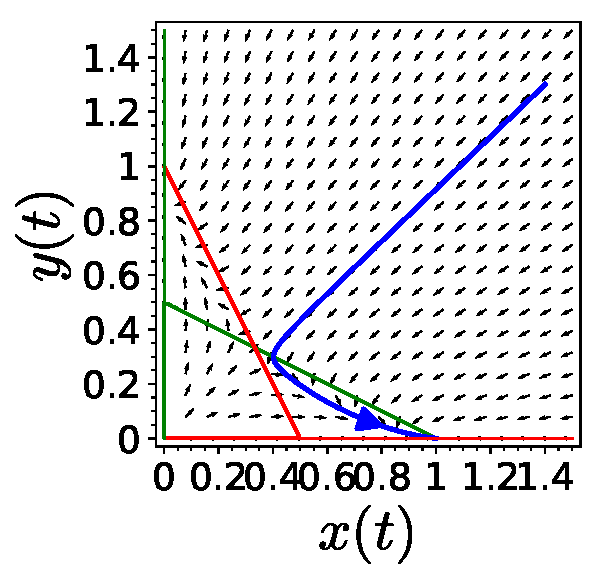
\includegraphics[width=\linewidth]{generated/sageplot/systems02-nullclines-competing-species-1.pdf}%
\end{image}%
\tcblower
\end{figureptx}%
In our example, we can plot the \(x\) and \(y\)-nullclines to help us understand our system (\hyperref[x:figure:systems02-figure-nullclines-competing-species-1]{Figure~{\xreffont\ref{x:figure:systems02-figure-nullclines-competing-species-1}}}). Of course, we have an equilibrium solution whenever an \(x\)-nullcline intersects with a \(y\)-nullcline. Thus, the equilibrium points for our particular system are \((0,0)\), \((1, 0)\), \((0, 1)\), and \((1/3, 1/3)\). Furthermore, we can choose a representative point in each region to find how the direction field is oriented. If we are given the  initial condition \((1.4, 1.3)\) for example, we can see that%
\begin{align*}
\frac{dx}{dt} & = -4.2\\
\frac{dy}{dt} & = -4.03.
\end{align*}
Since both of these numbers are negative, we can see that our initial trajectory is headed down and to the left\textemdash{}slightly more to the left than down. However, we have no guarantee that the trajectory will continue in this direction.%
\par
Before we proceed further with our analysis, let us determine what happens on the nullclines themselves. That is, we will examine the case when \(dx/dt = 0\) or \(dy/dt = 0\). If \(dx/dt = 0\), then any solution crossing this \(x\)-nullcline must be moving vertically. There can be no right or left movement at this point in the phase portrait. We can indicate this fact along with the direction of vertical movement by drawing a vertical slash with an arrow on the \(x\)-nullcline (\hyperref[x:figure:systems02-figure-nullclines-competing-species-1]{Figure~{\xreffont\ref{x:figure:systems02-figure-nullclines-competing-species-1}}}). For example, the point \((0.5, 0.25)\) lies on the \(x\)-nullcline and%
\begin{equation*}
\frac{dy}{dt}(0.5, 0.25) \lt 0.
\end{equation*}
Therefore, the trajectory that crosses the \(R\)-nullcline at \((0.5, 0.25)\) is moving down. As we move along the \(x\)-nullcline, the direction of this arrow can only change when we cross an \(y\)-nullcline.%
\par
Similarly, there can be no vertical motion on an \(y\)-nullcline. We will indicate the direction of horizontal motion by drawing a horizontal line with an arrow pointing to the right if \(dx/dt \gt 0\) on the \(y\)-nullcline and an arrow pointing to the left if \(dx/dt \lt 0\) on the \(y\)-nullcline.%
\par
We can also determine the basic direction of the solution curve by checking what happens at a point in each of the regions bounded by the nullclines. For example, at the point \((0.1, 0.1)\) we find that%
\begin{align*}
\frac{d}{dt}x(0.1, 0.1) & = 0.7\\
\frac{d}{dt}y(0.1, 0.1) & = 0.7.
\end{align*}
Thus, the general direction of any solution curve in this region is up and right (\hyperref[x:figure:systems02-figure-nullclines-competing-species-1]{Figure~{\xreffont\ref{x:figure:systems02-figure-nullclines-competing-species-1}}}).%
\par
What happens to the initial condition \((1.4, 1.3)\)? We see three possible scenarios if we follow the nullclines for large values of \(t\).%
\begin{itemize}[label=\textbullet]
\item{}Only species \(x\) survives and species \(y\) becomes extinct.%
\item{}Only species \(y\) survives and species \(x\) becomes extinct.%
\item{}There are essentially equal numbers of species \(x\) and \(y\).%
\end{itemize}
%
\end{example}
\begin{activity}{Plotting Direction Fields with Nullclines.}{g:activity:idp105545992613520}%
Consider the competing species model%
\begin{align*}
\frac{dx}{dt} & = x(1-x) - \beta xy\\
\frac{dy}{dt} & = y(1-y) - \beta xy,
\end{align*}
where the species interact weakly, say \(\beta = 1/2\).%
\begin{enumerate}[font=\bfseries,label=(\alph*),ref=\alph*]
\item{}Find the \(x\) and \(y\)-nullclines for this system.%
\item{}Find all equilibrium points for this system.%
\item{}The nullclines will divide the first quadrant of the plane,  \(x \geq 0\) and \(y \geq 0\), into different regions.  In each of these regions find a slope vector at some point \((x_0, y_0)\) in the region.  For example, at the point \((1,2)\), we can attach slope vector \((-1, -3)\).%
\item{}Sketch the phase plane for this system.%
\item{}If the initial populations are given by \(x(0) = 2.4\) and \(y(0) = 0.3\), what happens to the two populations as \(t \to \infty\)?%
\end{enumerate}
\end{activity}%
\begin{example}{}{g:example:idp105545992654608}%
There is no reason why our nullclines should be limited to straight lines. The system%
\begin{align*}
x' & = y - x^2\\
y' & = x - 2
\end{align*}
has an \(x\)-nullcline \(y = x^2\) and a \(y\)-nullcline \(x = 2\). These two nullclines intersect at \((2, 4)\), and the system has a single equilibrium solution. The nullclines divide the plane into four basic regions (\hyperref[x:figure:systems02-figure-nullclines-nonlinear]{Figure~{\xreffont\ref{x:figure:systems02-figure-nullclines-nonlinear}}}). By choosing a point in each of these regions and determining the direction of the slope field at that point, we can decide the direction of the slope field in the entire region.%
\begin{figureptx}{The system \(x' = y - x^2\) and \(y' = x - 2\)}{x:figure:systems02-figure-nullclines-nonlinear}{}%
\begin{image}{0.2}{0.6}{0.2}%
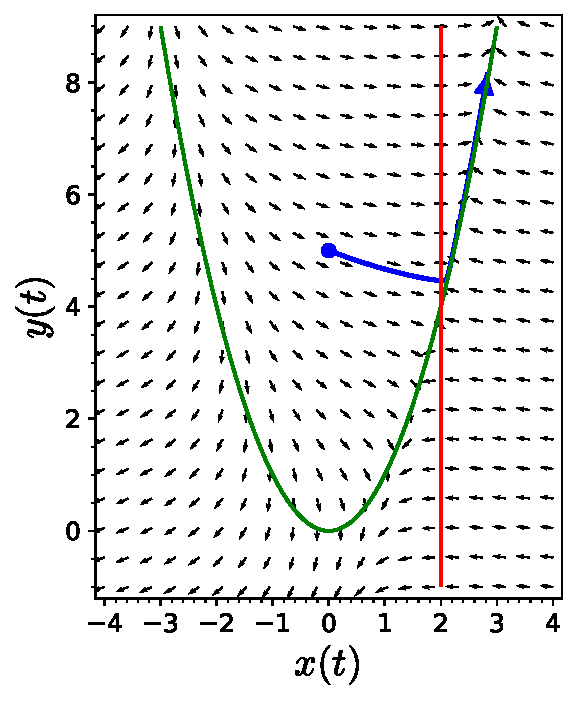
\includegraphics[width=\linewidth]{generated/sageplot/systems02-nullclines-nonlinear.pdf}%
\end{image}%
\tcblower
\end{figureptx}%
The only equilibrium solution of our system occurs at \((2, 4)\).%
\end{example}
\end{subsectionptx}
%
%
\typeout{************************************************}
\typeout{Subsection 2.2.4 Plotting Direction Fields with \emph{Sage}}
\typeout{************************************************}
%
\begin{subsectionptx}{Plotting Direction Fields with \emph{Sage}}{}{Plotting Direction Fields with \emph{Sage}}{}{}{x:subsection:systems02-subsection-sage-direction-fields}
It is easy to plot direction fields using \emph{Sage}. We can plot the direction field for the system%
\begin{align*}
x' & = y - 2x,\\
y' & = x - xy - x^3
\end{align*}
using the following \emph{Sage} interact. You can evaluate the cell below to get a menu driven applet for drawing direction fields for systems of two differential equations.%
\begin{figureptx}{A Sage applet for plotting direction fields for systems}{x:figure:systems02-figure-interactive-direction-fields}{}%
\centering
\setlength{\qrsize}{9em}
\setlength{\previewwidth}{\linewidth}
\addtolength{\previewwidth}{-\qrsize}
\begin{tcbraster}[raster columns=2, raster column skip=1pt, raster halign=center, raster force size=false, raster left skip=0pt, raster right skip=0pt]%
\begin{tcolorbox}[previewstyle, width=\previewwidth]%
\IfFileExists{generated/preview/systems02-interactive-direction-fields-preview.png}%
{\includegraphics[width=0.80\linewidth,height=\qrsize,keepaspectratio]{generated/preview/systems02-interactive-direction-fields-preview.png}}%
{\small{}Specify a static image with the \mono{@preview} attribute;\\%
Or create and provide an automatic screenshot as\\%
\mono{generated/preview/systems02-interactive-direction-fields-preview.png}\\%
via the \mono{PreTeXt-CLI} application or \mono{pretext/pretext} script.}%
\end{tcolorbox}%
\begin{tcolorbox}[qrstyle]%
{\hypersetup{urlcolor=black}\qrcode[height=\qrsize]{systems02-interactive-direction-fields.html}}%
\end{tcolorbox}%
\end{tcbraster}%
\tcblower
\end{figureptx}%
\end{subsectionptx}
%
%
\typeout{************************************************}
\typeout{Subsection 2.2.5 A Summary of Phase Plane Analysis}
\typeout{************************************************}
%
\begin{subsectionptx}{A Summary of Phase Plane Analysis}{}{A Summary of Phase Plane Analysis}{}{}{x:subsection:systems02-subsection-phase-plane-analysis}
We can use the following series of steps to summarize phase plane analysis for the nonlinear system%
\begin{align*}
\frac{dx}{dt} & = f(x, y)\\
\frac{dy}{dt} & = g(x, y).
\end{align*}
%
\begin{itemize}[label=\textbullet]
\item{}\emph{Step 1.} Draw the curves where \(f(x, y) = 0\). These curves are called the \terminology{\(x\)-nullclines}. When a solution curve \({\mathbf x}(t)\) lies on one of these curves, \(dx/dt = 0\), draw vertical slash marks on the \(x\)-nullclines to remind yourself that a trajectory crossing the nullcline can only do so if it is moving in a vertical direction at the instant of crossing.%
\item{}\emph{Step 2.} Draw the curves where \(g(x, y) = 0\). These curves are called the \terminology{\(y\)-nullclines}. When \({\mathbf x}(t)\) lies on one of these curves, \(dg/dt = 0\). Draw horizontal slash marks on the \(y\)-nullclines to remind yourself that a trajectory crossing the nullcline can only do so if it is moving in a horizontal direction at the instant of crossing.%
\item{}\emph{Step 3.} Label the points where the \(x\) and \(y\)-nullclines intersect. These intersections are the \terminology{equilibrium points}. If \({\mathbf x}(t)\) is ever at one of these points, then both \(dx/dt\) and \(dy/dt\) vanish. This means that the trajectory stays at the equilibrium point for all time. If our system is going to tend towards a steady state, then  \({\mathbf x}(t)\) will approach on of the equilibrium points as \(t \to \infty\).%
\item{}\emph{Step 4.} Label the regions of the \(xy\)-plane where \(dx/dt \lt 0\) and where \(dx/dt \gt 0\). These regions are always separated by \(x\)-nullclines.  Likewise, label the regions where \(dy/dt\) is positive and negative.%
\item{}\emph{Step 5.}Go back and put arrows on the vertical hash marks of the \(x\) nullclines. These arrows indicate whether the motion across the nullcline is up or down. The arrows are up on the parts of the \(x\)-nullclines that are in the \(dy/dt \gt 0\) region, and down on those parts of the \(x\)-nullclines in the \(dy/dt \lt 0\) regions. Likewise, draw arrows on the horizontal slash marks of the \(y\)-nullclines. These arrows are pointing right on the parts of the \(y\)-nullclines in the \(dx/dt \gt 0\) regions and left point on the parts in the \(dx/dt \lt 0\) regions.%
\item{}\emph{Step 6.}%
\begin{itemize}[label=$\circ$]
\item{}If \(dx/dt \gt 0\) and \(dy/dt \gt 0\), then both \(x(t)\) and \(y(t)\) are increasing and the trajectory moves up and right.%
\item{}If \(dx/dt \gt 0\) and \(dy/dt \lt 0\), the trajectory moves down and right.%
\item{}If \(dx/dt \lt 0\) and \(dy/dt \gt 0\), the trajectory moves up and left.%
\item{}If \(dx/dt \lt 0\) and \(dy/dt \lt 0\), the trajectory moves down and left.%
\end{itemize}
%
\end{itemize}
%
\end{subsectionptx}
%
%
\typeout{************************************************}
\typeout{Subsection 2.2.6 Important Lessons}
\typeout{************************************************}
%
\begin{subsectionptx}{Important Lessons}{}{Important Lessons}{}{}{x:subsection:systems02-subsection-important-lessons}
%
\begin{itemize}[label=\textbullet]
\item{}The righthand side of the system%
\begin{align*}
\frac{dx}{dt} & = f(x, y)\\
\frac{dy}{dt} & = g(x, y)
\end{align*}
can be viewed as a vector field, \((f(x,y), g(x,y))\), which can be plotted in the \(x,y\)-plane.%
\item{}Competition between two competing species can be modeled with the system%
\begin{align*}
\frac{dx}{dt} & = \alpha x \left(1 - \frac{x}{M} \right) - \beta xy\\
\frac{dy}{dt} & = \gamma y \left(1 - \frac{y}{N} \right) - \delta xy.
\end{align*}
%
\item{}We can use nullclines and phase plane analysis to sketch solution curves for the system%
\begin{align*}
\frac{dx}{dt} & = f(x, y)\\
\frac{dy}{dt} & = g(x, y).
\end{align*}
%
\end{itemize}
%
\end{subsectionptx}
%
%
\typeout{************************************************}
\typeout{Reading Questions 2.2.7 Reading Questions}
\typeout{************************************************}
%
\begin{reading-questions-subsection}{Reading Questions}{}{Reading Questions}{}{}{x:reading-questions:reading-questions-system02}
\begin{divisionexercise}{1}{}{}{x:exercise:reading-questions-system02-1}%
Using your own words, explain what a nullcline is.%
\end{divisionexercise}%
\begin{divisionexercise}{2}{}{}{x:exercise:reading-questions-system02-2}%
What happens at the intersection of an \(x\)-nullcline and a \(y\)-nullcline?%
\end{divisionexercise}%
\end{reading-questions-subsection}
%
%
\typeout{************************************************}
\typeout{Exercises 2.2.8 Exercises}
\typeout{************************************************}
%
\begin{exercises-subsection}{Exercises}{}{Exercises}{}{}{x:exercises:systems02-exercises}
\begin{divisionexercise}{1}{}{}{g:exercise:idp105545992672656}%
Consider a cooperating species model%
\begin{align*}
\frac{dx}{dt} & = x(1-x) + \beta xy\\
\frac{dy}{dt} & = y(1-y) + \beta xy,
\end{align*}
where the species interact weakly, say \(\beta = 1/2\).%
\begin{enumerate}[label=(\alph*)]
\item{}Find the \(x\) and \(y\)-nullclines for this system.%
\item{}Find all equilibrium points for this system.%
\item{}Sketch the phase plane for this system.%
\item{}If the initial populations are given by \(x(0) = 2.4\) and \(y(0) = 0.3\), what happens to the two populations as \(t \to \infty\)?%
\end{enumerate}
%
\end{divisionexercise}%
\begin{divisionexercise}{2}{}{}{g:exercise:idp105545992677904}%
For the following two systems of equations%
\begin{itemize}[label=\textbullet]
\item{}Find the equilibrium points of the system.%
\item{}Sketch the phase plane and direction field for each system using technology.%
\item{}Briefly describe the behavior of typical solutions.%
\end{itemize}
%
\begin{enumerate}[label=(\alph*)]
\item{}%
\begin{align*}
x' & = \cos y\\
y' & = -x + y
\end{align*}
%
\item{}%
\begin{align*}
x' & = y\\
y' & = x - x^3 -y
\end{align*}
%
\end{enumerate}
%
\end{divisionexercise}%
\begin{divisionexercise}{3}{}{}{g:exercise:idp105545992681744}%
Consider an epidemic that moves through an isolated population.  We will make the following assumptions about the epidemic.%
\begin{itemize}[label=\textbullet]
\item{}Individuals are infected at a rate proportional to the product of the number of infected and susceptible individuals.  We assume that the constant of proportionality is \(\alpha\).%
\item{}The length of the incubation period is negligible, and infectious individuals are immediately infectious.%
\item{}On the average, an infected individual dies after 10 days.%
\item{}Only a single individual is initially ill.%
\item{}Infected individuals do not give birth, but susceptible individuals have a birth rate of 0.0003 per individual per year.  Newborns are susceptible.%
\end{itemize}
If \(S(t)\) is the number of susceptible and \(I(t)\) is the number of infected people, then%
\begin{align}
\frac{dS}{dt} & = -\alpha SI + 0.0003S\label{x:mrow:systems02-equation-epidemic-1}\\
\frac{dI}{dt} & = \alpha SI - 0.1I.\label{x:mrow:systems02-equation-epidemic-2}
\end{align}
%
\par
The constant \(\alpha\) is a measure of the relative infectivity of the disease.  Some diseases such as Ebola, a viral hemorrhagic fever, are extremely infectious with a mortaility rate of up to 90\%. On the other hand, AIDS which is caused by the HIV virus, has a much lower transmission rate.  The goal of this exercise is to examine the differences between the two.%
\begin{enumerate}[label=(\alph*)]
\item{}If \(\alpha = 0.05\), draw the phase portrait.  Be sure to label all nullclines and equilibrium solutions.  Suppose that \(S(0) = 1000\) and \(I(0) = 1\).  What happens to the solution curve as \(t \to \infty\)?%
\item{}If \(\alpha = 0.000001\), draw the phase portrait.  Be sure to label all nullclines and equilibrium solutions.  Suppose that \(S(0) = 30000\) and \(I(0) = 1\).  What happens to the solution curve as \(t \to \infty\)?%
\item{}What conclusions can you draw about the behavior of the two different epidemics?%
\end{enumerate}
%
\end{divisionexercise}%
\end{exercises-subsection}
%
%
\typeout{************************************************}
\typeout{Subsection 2.2.9 Plotting Nullclines with \emph{Sage}}
\typeout{************************************************}
%
\begin{subsectionptx}{Plotting Nullclines with \emph{Sage}}{}{Plotting Nullclines with \emph{Sage}}{}{}{x:subsection:subsection-sytems02-sage}
Let us use \emph{Sage} to analyze the system%
\begin{align*}
x' & = x + y,\\
y' & = -2x + y.
\end{align*}
First let us plot the phase plane of the system without nullclines.%
\begin{sageinput}
x, y, t = var('x y t')
F = [x + y, -2*x + y]
P = desolve_system_rk4(F,[x, y],ics=[0,0.55,0],ivar=t,end_points=10,step=0.01)
Q = [ [j,k] for i,j,k in P]
p = line(Q, axes_labels=['$x(t)$','$y(t)$'], thickness=2)
n = sqrt(F[0]^2 + F[1]^2)
F_unit = [F[0]/n, F[1]/n] #set all vectors in the vector field to be same length
p += plot_vector_field(F_unit, (x,-4,4), (y,-4,4), axes_labels=['$x(t)$','$y(t)$'], xmax = 4, xmin = -4, ymax = 4, ymin = -4, aspect_ratio=1)
p
\end{sageinput}
\begin{sageoutput}

\end{sageoutput}
If these \emph{Sage} commands seem unfamiliar, you may want to refer to \hyperref[x:subsection:systems01-subsection-sage]{Subsection~{\xreffont\ref{x:subsection:systems01-subsection-sage}}}%
\par
We can add nullclines to our plot using the \mono{implicit\_plot} function from \emph{Sage}.%
\begin{sageinput}
x, y, t = var('x y t')
F = [x + y, -2*x + y]
P = desolve_system_rk4(F,[x, y],ics=[0,0.55,0],ivar=t,end_points=10,step=0.01)
Q = [ [j,k] for i,j,k in P]
p = line(Q, axes_labels=['$x(t)$','$y(t)$'], thickness=2)
n = sqrt(F[0]^2 + F[1]^2)
F_unit = [F[0]/n, F[1]/n] #set all vectors in the vector field to be same length
p += plot_vector_field(F_unit, (x,-4,4), (y,-4,4), axes_labels=['$x(t)$','$y(t)$'], xmax = 4, xmin = -4, ymax = 4, ymin = -4, aspect_ratio=1)
p += implicit_plot(F[0], (x,-4,4), (y,-4,4), color="green")
p += implicit_plot(F[1], (x,-4,4), (y,-4,4), color="red")
p
\end{sageinput}
\begin{sageoutput}

\end{sageoutput}
The \(x\)-nullclines are plotted in green and the \(y\)-nullclines are in red.%
\end{subsectionptx}
\end{sectionptx}
%
%
\typeout{************************************************}
\typeout{Section 2.3 Numerical Techniques for Systems}
\typeout{************************************************}
%
\begin{sectionptx}{Numerical Techniques for Systems}{}{Numerical Techniques for Systems}{}{}{x:section:systems03}
\begin{objectives}{Objectives}{g:objectives:idp105545992732944}
%
\begin{itemize}[label=\textbullet]
\item{}To understand that many systems of equations cannot be solved analytically but can be solved using numerical techniques such as \terminology{Euler's Method} or \terminology{Runge-Kutta methods} to find approximate solutions for the system.%
\item{}To understand that we are guaranteed unique local solutions to any system of first-order differential equations provided certain condtions are met.%
\item{}To understand that uniqueness tells us that two distinct solutions cannot start at the same place nor can solutions intersect.%
\item{}To understand that solutions do not depend on time in an autonomous system.%
\end{itemize}
\end{objectives}
\begin{introduction}{}%
If we are unable to find an analytic solution to a first-order differential equation \(y' = f(t, y)\), there is no reason to expect that it will be any easier to solve a system of equations. However, many of the numerical techniques that are used to solve a first-order equation can be extended to solve a system.%
\end{introduction}%
%
%
\typeout{************************************************}
\typeout{Subsection 2.3.1 Duffing's Equation}
\typeout{************************************************}
%
\begin{subsectionptx}{Duffing's Equation}{}{Duffing's Equation}{}{}{x:subsection:systems03-subsection-duffing}
Large mobile cranes can reach up to 700 feet (\hyperref[x:figure:systems03-figure-cranes]{Figure~{\xreffont\ref{x:figure:systems03-figure-cranes}}}). This is about the same height as a 50 story building. At such heights, cranes are susceptible to winds and the end of the boom can move back and forth several feet even in moderate winds. We can model the motion as a harmonic oscillator if the side-to-side motion is not too great. However, if the wind becomes too strong and the crane moves too much, gravity will become a factor and the crane may topple due to its weight.%
\begin{figureptx}{Cranes}{x:figure:systems03-figure-cranes}{}%
\begin{image}{0.2}{0.6}{0.2}%
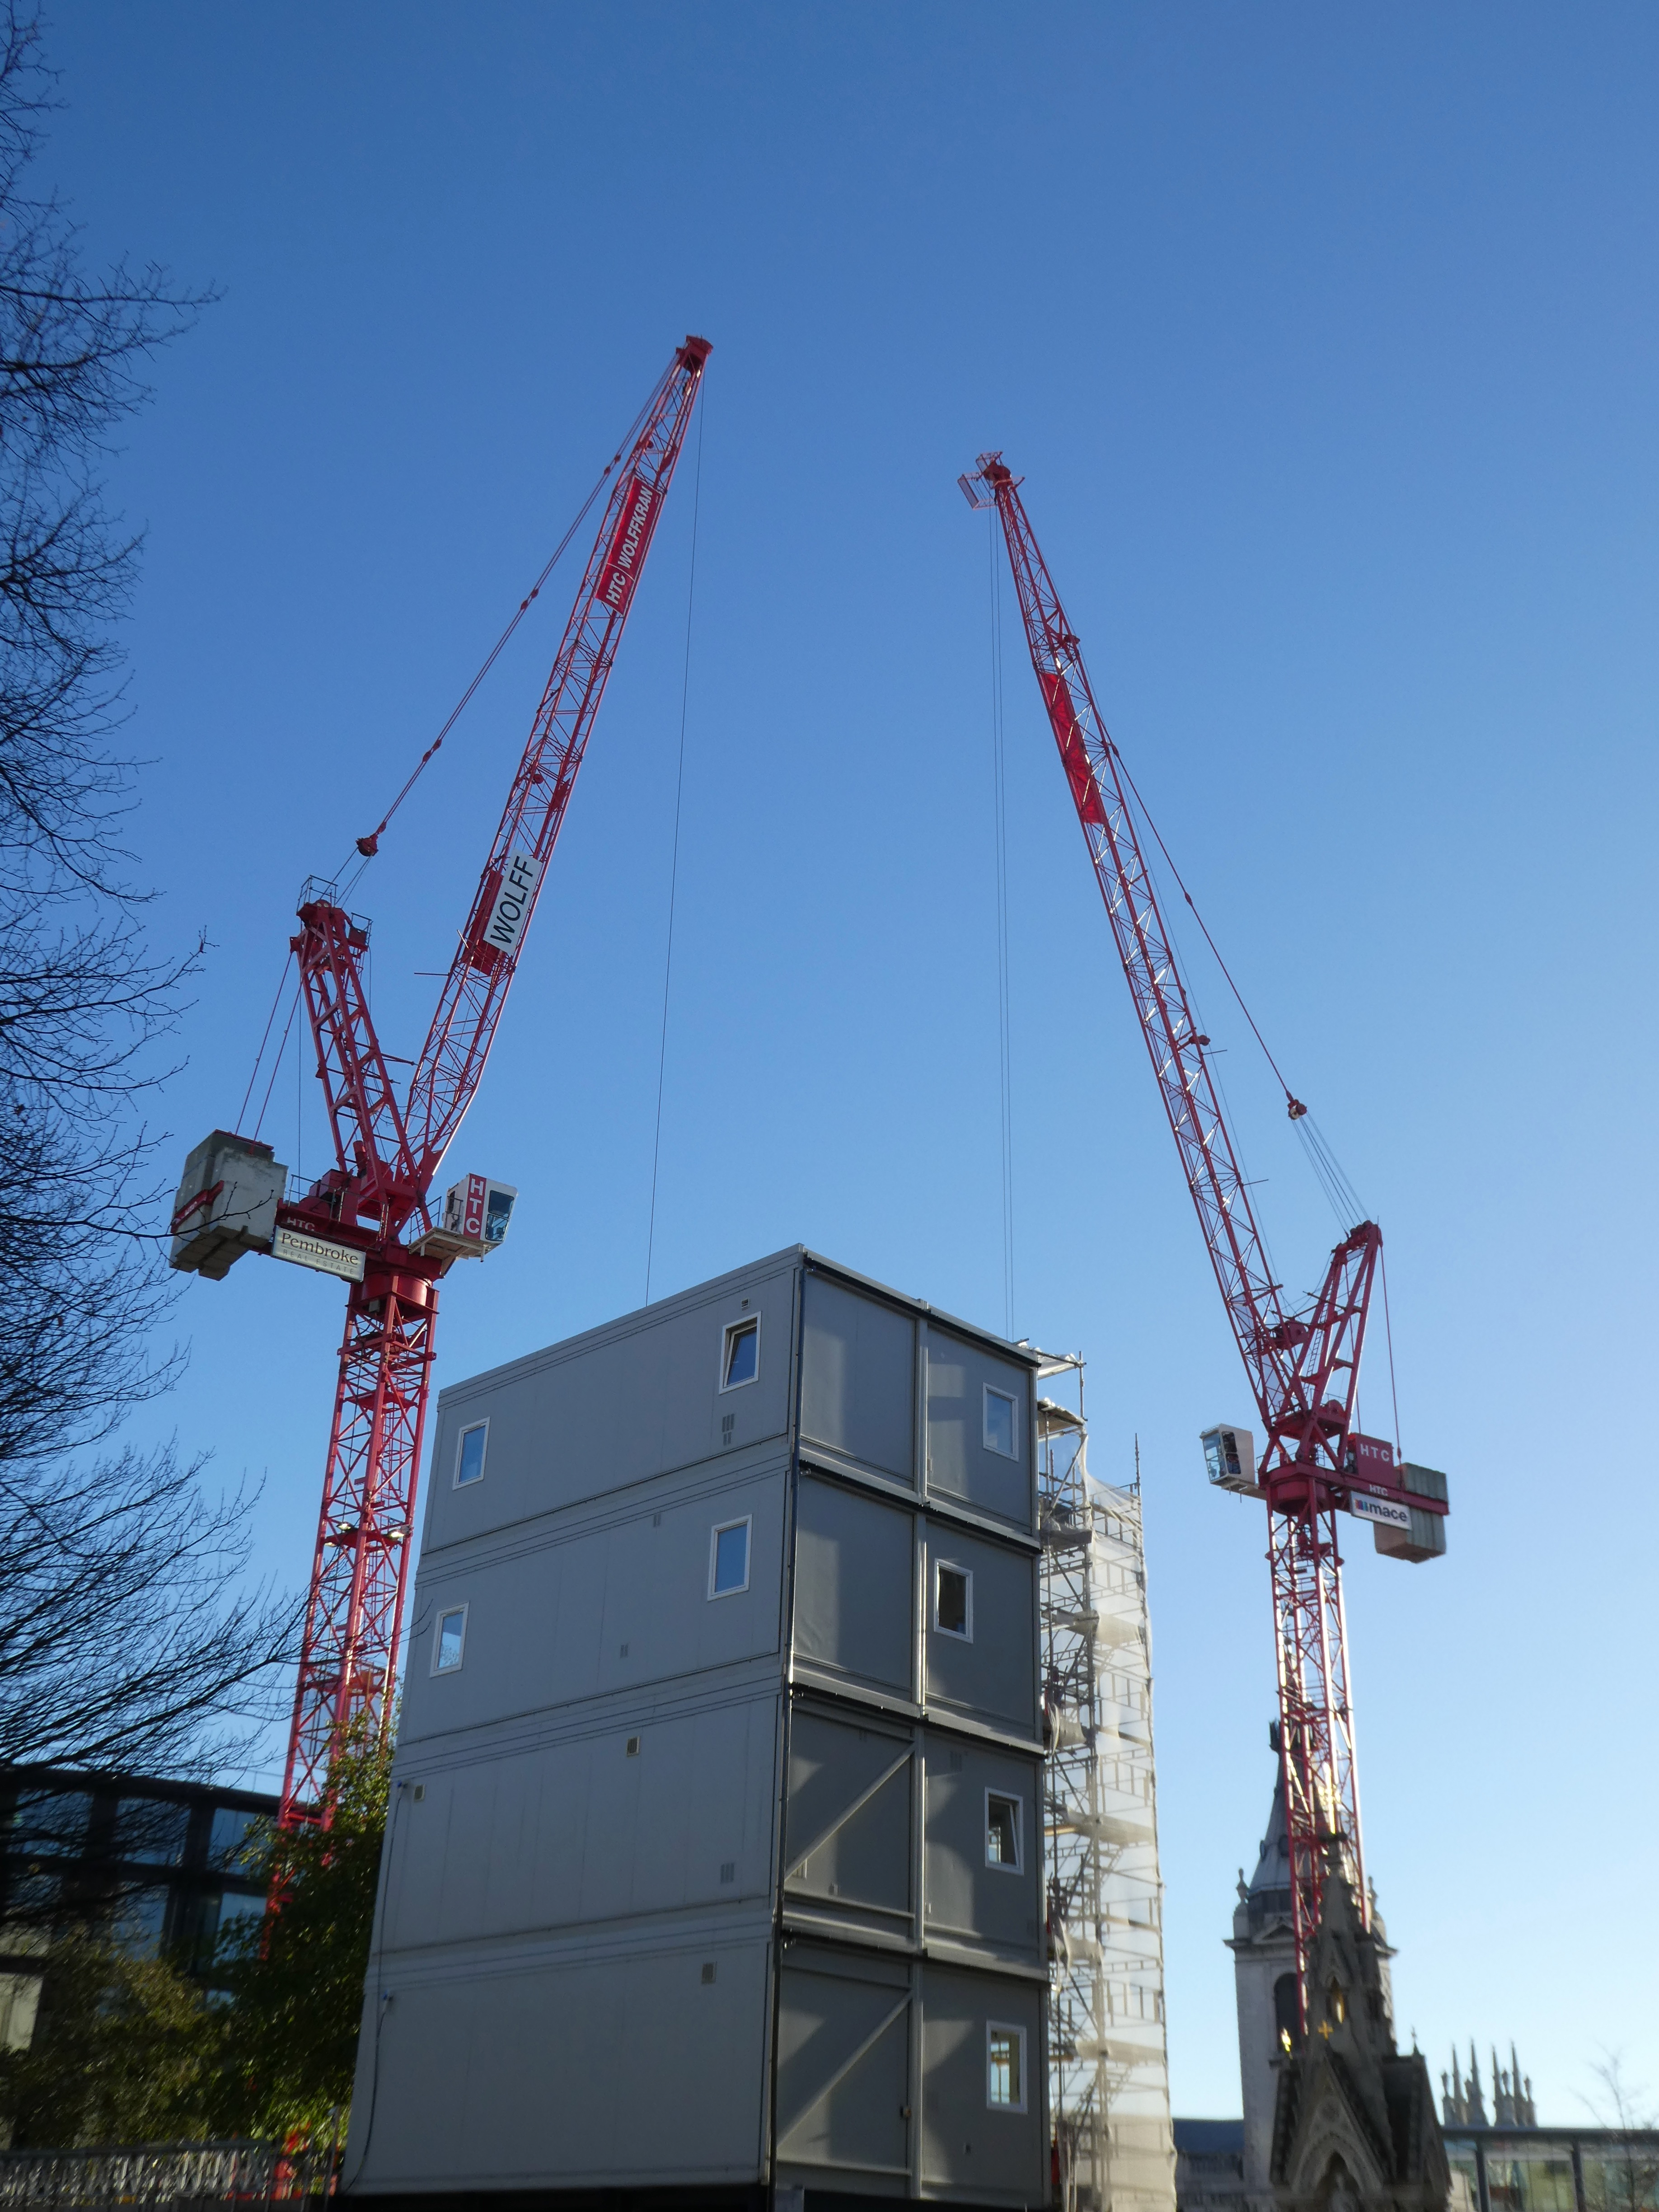
\includegraphics[width=\linewidth]{external/images/cranes-london.jpg}
\end{image}%
\tcblower
\end{figureptx}%
Before we can construct a model that might best describe the swaying of a large crane, we should remind ourselves of how harmonic oscillators work (see \hyperref[x:section:firstlook01]{Section~{\xreffont\ref{x:section:firstlook01}}}). A simple mass-spring system can be modeled by the equation%
\begin{equation*}
m \frac{d^2 x}{dt^2} = - kx,
\end{equation*}
where \(x = x(t)\) is the displacement of the mass at time \(t\). Given such a system, the mass will oscillate forever with constant amplitude. If we want to be a bit more realistic, we can introduce a damping force,%
\begin{equation*}
-b \frac{dx}{dt},
\end{equation*}
where \(b \gt 0\).  Our equation now becomes%
\begin{equation*}
m \frac{d^2 x}{dt^2} = - kx - b \frac{dx}{dt}.
\end{equation*}
If we let \(p = b/m\) and \(q = k/m\), we can rewrite this last equation as%
\begin{equation*}
\frac{d^2 x}{dt^2} + p \frac{dx}{dt} + q x = 0.
\end{equation*}
If we set \(v = x'\), we can rewrite this second-order equation as a system of first-order equations,%
\begin{align*}
\frac{dx}{dt} & = v,\\
\frac{dv}{dt} & = - qx - pv.
\end{align*}
%
\par
In the case of our swaying crane, we will let \(x = x(t)\) be the displacement of the end of the boom from the perfect vertical position. When \(x(t) \neq 0\), the boom is bent, and the structure of the boom supplies a strong restorative force to bring everything back to a true vertical position. Thus, the swaying of our crane's boom might be described by an equation such as%
\begin{equation*}
\frac{d^2 x}{dt^2} + 0.1 \frac{dx}{dt} + 0.3 x = 0
\end{equation*}
or the equivalent system,%
\begin{align*}
\frac{dx}{dt} & = v,\\
\frac{dv}{dt} & = - 0.3 x - 0.1 v.
\end{align*}
We will learn how to solve such systems later, but it is easy to check that%
\begin{equation*}
x(t) =  c_1 e^{-t/20} \cos \left(\frac{\sqrt{119}}{20} t\right) + c_2 e^{-t/20} \sin \left(\frac{\sqrt{119}}{20} t\right)
\end{equation*}
is a solution to our equation. The \emph{Sage} code for solving this system is given below.%
\begin{sageinput}
t = var('t')
x = function('x')(t)
b = 0.1
k = 0.3
position = desolve(diff(x,t,2)+b*diff(x,t)+ k*x == 0,x)
velocity = diff(position, t)
position.show()
velocity.show()
\end{sageinput}
\begin{sageoutput}

\end{sageoutput}
The constants \(c_1\) and \(c_2\) can be determined if we know the initial position and initial velocity of the end of the crane's boom. We show several solutions to our equation in \hyperref[x:figure:systems03-figure-solutions-crane]{Figure~{\xreffont\ref{x:figure:systems03-figure-solutions-crane}}}.%
\begin{figureptx}{Solutions to \(x'' + 0.1x' + 0.3 x = 0\)}{x:figure:systems03-figure-solutions-crane}{}%
\begin{image}{0.2}{0.6}{0.2}%
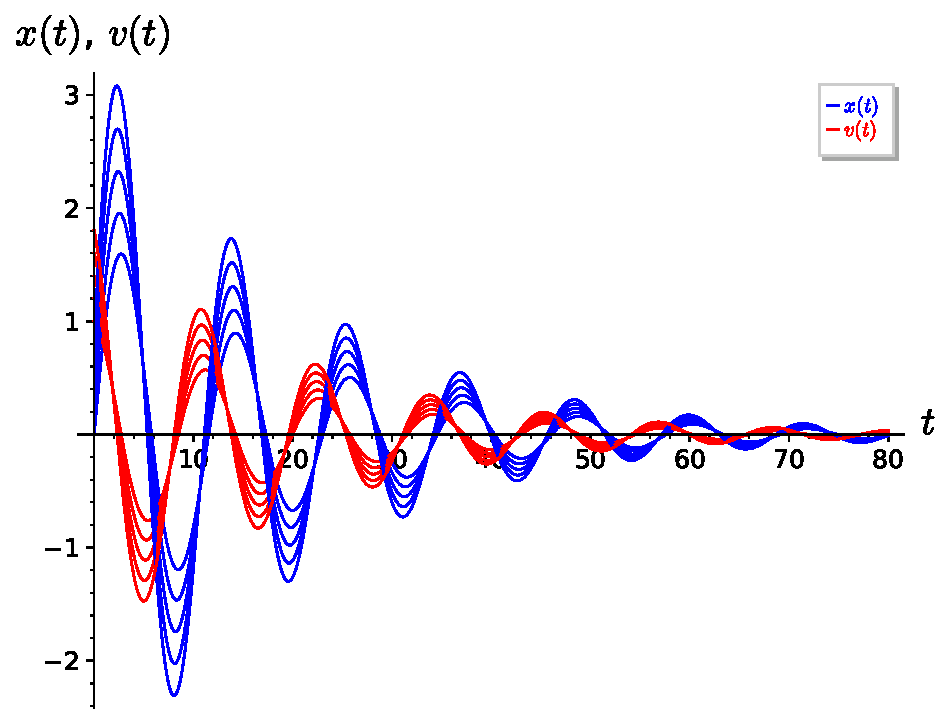
\includegraphics[width=\linewidth]{generated/sageplot/systems03-solutions-crane.pdf}%
\end{image}%
\tcblower
\end{figureptx}%
Modeling the swaying motion of a crane with a harmonic oscillator might work only if the side-to-side motion is small. If the motion is larger, we must account for the effect of gravity in our model. When \(x(t)\) is large, part of the crane will not be above any other part of the crane. Thus, gravity will pull downward on that part of the crane and will cause the crane to bend even further. We can model this effect by setting the equation for our harmonic oscillator equal to a factor of \(x^3\),%
\begin{equation}
\frac{d^2 x}{dt^2}  + 0.1 \frac{dx}{dt} + 0.3 x = 0.02 x^3.\label{x:men:systems03-equation-duffing}
\end{equation}
When \(x\) is small, this forcing term will not contribute much to the motion of the building. However, when \(x\) is large, the term will contribute a great deal. The equation \(x'' + 0.1 x' + 0.3 x = 0.02 x^3\) is an example of \terminology{Duffing's equation}\index{Duffing's equation}.%
\par
We can rewrite equation~\hyperref[x:men:systems03-equation-duffing]{({\xreffont\ref{x:men:systems03-equation-duffing}})} as a system of first-order differential equations by letting \(dx/dt = v\),%
\begin{align}
\frac{dx}{dt} \amp = v\label{x:mrow:systems03-equation-duffing-system-1}\\
\frac{dv}{dt} \amp = - 0.1 v - 0.3 x + 0.02 x^3.\label{x:mrow:systems03-equation-duffing-system-2}
\end{align}
Thus, one of our main objectives should be finding and analyzing solutions to such a system.%
\end{subsectionptx}
%
%
\typeout{************************************************}
\typeout{Subsection 2.3.2 Euler's Method for Systems}
\typeout{************************************************}
%
\begin{subsectionptx}{Euler's Method for Systems}{}{Euler's Method for Systems}{}{}{x:subsection:systems03-subsection-eulers-method}
The system of equations \hyperref[x:mrow:systems03-equation-duffing-system-1]{({\xreffont\ref{x:mrow:systems03-equation-duffing-system-1}})}\textendash{}\hyperref[x:mrow:systems03-equation-duffing-system-2]{({\xreffont\ref{x:mrow:systems03-equation-duffing-system-2}})} is nonlinear due the \(x^3\) term. There is little hope to finding an analytic solution to such a system. We can use software to plot the phase plane in order to learn something about the solutions (\hyperref[x:figure:systems03-figure-duffings-equation-phase-plane]{Figure~{\xreffont\ref{x:figure:systems03-figure-duffings-equation-phase-plane}}}). However, we still need to numerically generate solutions in order to plot the phase plane.%
\begin{figureptx}{The phase plane for Duffing's equation}{x:figure:systems03-figure-duffings-equation-phase-plane}{}%
\begin{image}{0.2}{0.6}{0.2}%
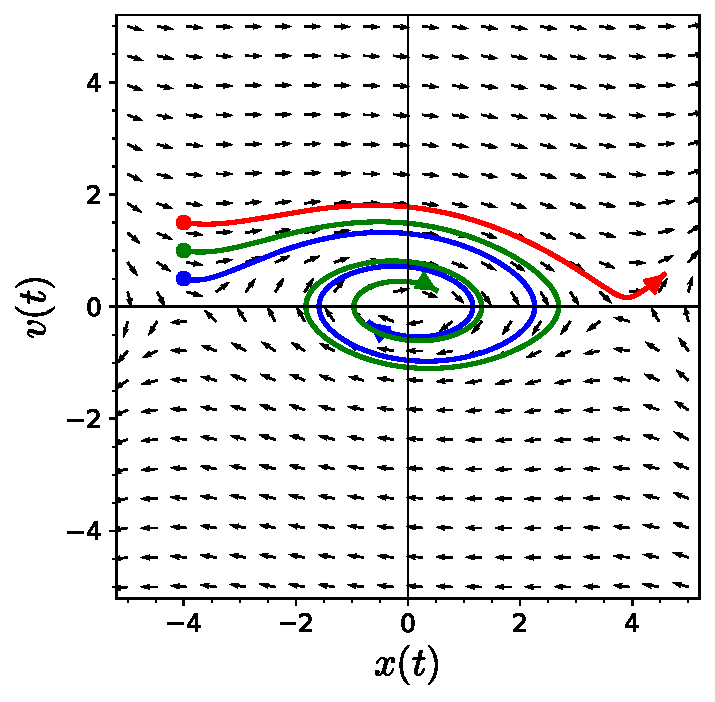
\includegraphics[width=\linewidth]{generated/sageplot/systems03-duffings-equation-phase-plane.pdf}%
\end{image}%
\tcblower
\end{figureptx}%
Let us see how we might find a numerical solution for a system. Consider the system%
\begin{align*}
\frac{dx}{dt} & = f(t, x, y)\\
\frac{dy}{dt} & = g(t, x, y),
\end{align*}
with initial conditions \(x(t_0) = x_0\) and \(y(t_0) = y_0\). We can rewrite our system in vector form%
\begin{align*}
\frac{d {\mathbf x}}{dt} & = {\mathbf f}(t, {\mathbf x})\\
{\mathbf x}(t_0) & = {\mathbf x}_0
\end{align*}
where \({\mathbf x} = (x, y)\), \(d{\mathbf x}/dt = (dx/dt, dy/dt)\), \({\mathbf f} = (f, g)\), and \({\mathbf x}_0 = (x_0, y_0)\). We wish to find approximate values \(x_1, x_2, \ldots, x_n\) and \(y_1, y_2, \ldots, y_n\) for the solution \(x(t)\) and \(y(t)\) at the points%
\begin{equation*}
t_k = t_0 + kh, \qquad k = 1, 2, \ldots, n,
\end{equation*}
where \(h\) is the step size. If we let \({\mathbf x}_k = (x_k, y_k)\) and \({\mathbf f}_k = (f(x_k, y_k ), g(x_k, y_k ))\), then Euler's method now becomes%
\begin{equation*}
{\mathbf x}_{k + 1} = {\mathbf x}_k + h {\mathbf f}_k
\end{equation*}
or%
\begin{align*}
x_{k + 1} & = x_k + h f(t_k, x_k, y_k)\\
y_{k + 1} & = y_k + h g(t_k, x_k, y_k).
\end{align*}
The initial conditions are used to determine \({\mathbf f}_0\), which is the tangent vector to the graph of the solution \(\mathbf x(t)\) in the \(xy\)-plane (\hyperref[x:figure:systems03-figure-duffings-equation-phase-plane]{Figure~{\xreffont\ref{x:figure:systems03-figure-duffings-equation-phase-plane}}}). We can move in the direction of this tangent vector for time \(h\) in order to find the next point \({\mathbf x}_1\). We then calculate a new tangent vector \({\mathbf f}_1\) and then move along this new vector for a time step \(h\) to find \({\mathbf x}_2\). We can repeat this technique to generate an approximate solution curve in the phase plane.%
\begin{example}{Numerical Solutions for Duffing's Equation.}{g:example:idp105545992477456}%
We are now in a position to calculate some solutions to Duffing's equation. Suppose that%
\begin{align*}
\frac{dx}{dt} & = v,\\
\frac{dv}{dt} & = - 0.3 x + 0.02x^3 - 0.1 v,
\end{align*}
with initial conditions \((t_0, x_0, v_0) = (0, 0, 1.7652)\).  Using a numerical algorithm, we can generate enough points to generate a graph of the solution (\hyperref[x:figure:systems03-figure-duffings-equation-solutions-1]{Figure~{\xreffont\ref{x:figure:systems03-figure-duffings-equation-solutions-1}}}).%
\begin{figureptx}{Solutions for Duffing's equation with initial conditions \(x(0) = 0\) and \(v(0) = 1.7652\)}{x:figure:systems03-figure-duffings-equation-solutions-1}{}%
\begin{image}{0.2}{0.6}{0.2}%
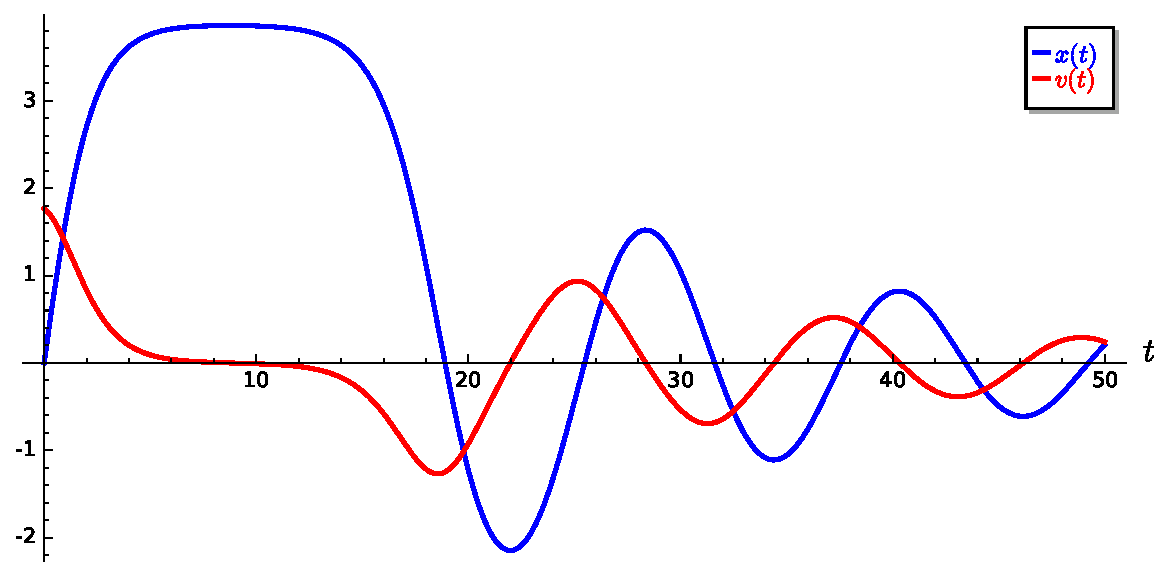
\includegraphics[width=\linewidth]{generated/sageplot/systems03-duffings-equation-solutions-1.pdf}%
\end{image}%
\tcblower
\end{figureptx}%
The surprising thing about Duffing's equation is that it is extremely sensitive to initial conditions. A slight change in the initial conditions can yield dramatically different solutions. If we change the initial velocity to \(v(0) = 1.7653\), we obtain a very different graph of the solution (\hyperref[x:figure:systems03-figure-duffings-equation-solutions-1]{Figure~{\xreffont\ref{x:figure:systems03-figure-duffings-equation-solutions-1}}} ).  For small initial velocities, solutions spiral towards the origin. However, a larger initial velocity will send the solution in the phase plane away from the origin. If the crane sways too violently, we will have a disaster.%
\begin{figureptx}{Solutions for Duffing's equation with initial conditions \(x(0) = 0\) and \(v(0) = 1.7653\)}{x:figure:systems03-figure-duffings-equation-solutions-2}{}%
\begin{image}{0.2}{0.6}{0.2}%
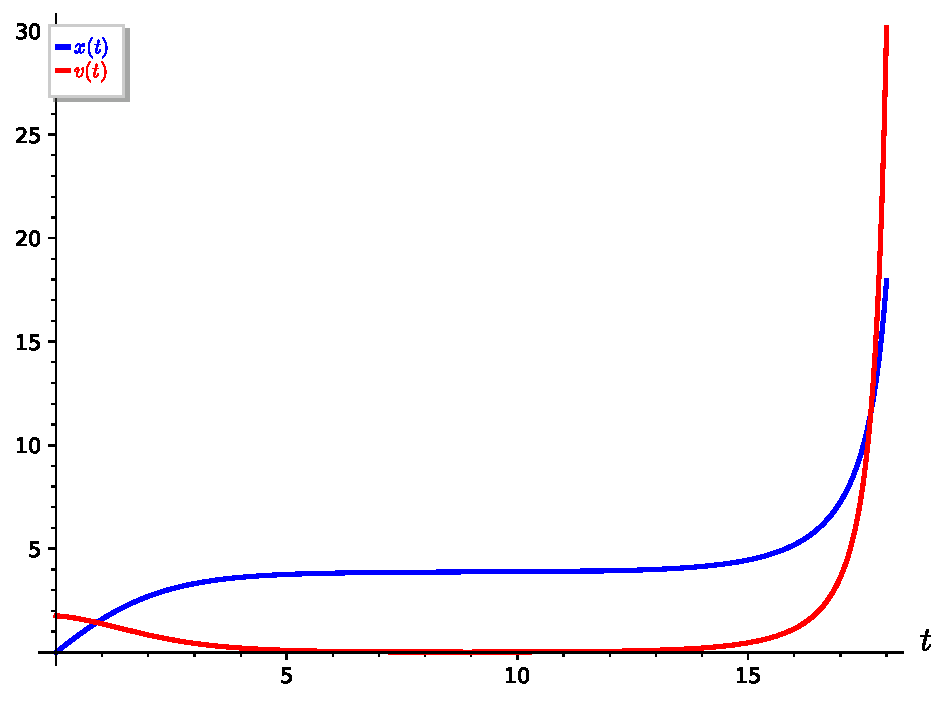
\includegraphics[width=\linewidth]{generated/sageplot/systems03-duffings-equation-solutions-2.pdf}%
\end{image}%
\tcblower
\end{figureptx}%
\end{example}
\begin{example}{}{g:example:idp105545992484752}%
Let us consider the system%
\begin{align*}
x' & = x - y + t\\
y' & = -x + y^2 - t^2\\
x(0) & = 1\\
y(0) & = 0.
\end{align*}
Then \((x_0, y_0) = (1, 0)\).  Letting the step size be \(h = 0.1\), we obtain and%
\begin{align*}
\begin{pmatrix}
x_1 \\ y_1
\end{pmatrix}
& =
\begin{pmatrix}
x_0 \\ y_0
\end{pmatrix}
+ h
\begin{pmatrix}
f(t_0, x_0, y_0) \\  g(t_0, x_0, y_0)
\end{pmatrix}\\
& =
\begin{pmatrix}
1 \\ 0
\end{pmatrix}
+
(0.1)
\begin{pmatrix}
1 \\ -1
\end{pmatrix}\\
& =
\begin{pmatrix}
1.1 \\ -0.1
\end{pmatrix}.
\end{align*}
Similarly,%
\begin{align*}
\begin{pmatrix}
x_2 \\ y_2
\end{pmatrix}
& =
\begin{pmatrix}
x_1 \\ y_1
\end{pmatrix}
+ h
\begin{pmatrix}
f(t_1, x_1, y_1) \\  g(t_1, x_1, y_1)
\end{pmatrix}\\
& =
\begin{pmatrix}
1.1 \\ -0.1
\end{pmatrix}
+
(0.1)
\begin{pmatrix}
1.3 \\ -1.1
\end{pmatrix}\\
& =
\begin{pmatrix}
1.23 \\ -0.21
\end{pmatrix}.
\end{align*}
Using this procedure, we can generate a list of values that will approximate the solution to our system (\hyperref[x:table:systems03-table-euler-approximation]{Table~{\xreffont\ref{x:table:systems03-table-euler-approximation}}}).%
\begin{tableptx}{\textbf{Euler's approximation for a system of equations}}{x:table:systems03-table-euler-approximation}{}%
\centering%
{\tabularfont%
\begin{tabular}{cccccc}\hrulemedium
\(k\)&\(t_k\)&\(x_k\)&\(hf(t_k, x_k, y_k)\)&\(y_k\)&\(hg(t_k, x_k, y_k)\)\tabularnewline\hrulemedium
\(0\)&\(0.0\)&\(1.0000\)&\(0.1000\)&\(0.0000\)&\(-0.1000\)\tabularnewline[0pt]
\(1\)&\(0.1\)&\(1.1000\)&\(0.1300\)&\(-0.1000\)&\(-0.1100\)\tabularnewline[0pt]
\(2\)&\(0.2\)&\(1.2300\)&\(0.1640\)&\(-0.2100\)&\(-0.1226\)\tabularnewline[0pt]
\(3\)&\(0.3\)&\(1.3940\)&\(0.2027\)&\(-0.3326\)&\(-0.1373\)\tabularnewline[0pt]
\(4\)&\(0.4\)&\(1.5967\)&\(0.2467\)&\(-0.4699\)&\(-0.1536\)\tabularnewline[0pt]
\(5\)&\(0.5\)&\(1.8433\)&\(0.2967\)&\(-0.6235\)&\(-0.1705\)\tabularnewline[0pt]
\(6\)&\(0.6\)&\(2.1400\)&\(0.3534\)&\(-0.7940\)&\(-0.1870\)\tabularnewline[0pt]
\(7\)&\(0.7\)&\(2.4934\)&\(0.4174\)&\(-0.9809\)&\(-0.2021\)\tabularnewline[0pt]
\(8\)&\(0.8\)&\(2.9108\)&\(0.4894\)&\(-1.1830\)&\(-0.2151\)\tabularnewline[0pt]
\(9\)&\(0.9\)&\(3.4002\)&\(0.5698\)&\(-1.3982\)&\(-0.2255\)\tabularnewline[0pt]
\(10\)&\(1.0\)&\(3.9701\)&\(0.6594\)&\(-1.6237\)&\(-0.2334\)\tabularnewline\hrulemedium
\end{tabular}
}%
\end{tableptx}%
Notice that our system is not autonomous and depends on time. Therefore, we cannot graph the phase plane of this system; however, we can graph a solution curve in three dimensions (\hyperref[x:figure:systems03-figure-euler]{Figure~{\xreffont\ref{x:figure:systems03-figure-euler}}}).%
\begin{figureptx}{A solution curve for Duffing's equation}{x:figure:systems03-figure-euler}{}%
\begin{image}{0.25}{0.5}{0.25}%
\includegraphics[width=\linewidth]{generated/asymptote/figure-euler.pdf}
\end{image}%
\tcblower
\end{figureptx}%
\end{example}
\begin{activity}{Solving a System Numerically.}{g:activity:idp105545992522000}%
Consider the system%
\begin{align*}
x' & = 2x\\
y' & = y
\end{align*}
with initial conditions \(x(0) = 1\) and \(y(0) = 3\).\footnotemark{}%
\begin{enumerate}[font=\bfseries,label=(\alph*),ref=\alph*]
\item{}Show that \({\mathbf x}(t) = (e^{2t}, 3e^t)\) satisfies the initial value problem.%
\item{}Use Euler's method with step size \(\Delta t = 0.5\) to approximate this solution, and check how close the approximation is to the real solution when \(t = 2\), \(t = 4\), and \(t = 6\).%
\item{}Use Euler's method with step size \(\Delta t = 0.1\) to approximate this solution, and check how close the approximation is to the real solution when \(t = 2\), \(t = 4\), and \(t = 6\).%
\item{}Discuss how and why the Euler approximations differ from the real solution.%
\end{enumerate}
\end{activity}%
\footnotetext[1]{You will find Sage very useful for this exercise\label{g:fn:idp105545992557072}}%
\end{subsectionptx}
%
%
\typeout{************************************************}
\typeout{Subsection 2.3.3 Taylor Series Methods}
\typeout{************************************************}
%
\begin{subsectionptx}{Taylor Series Methods}{}{Taylor Series Methods}{}{}{x:subsection:systems03-subsection-taylor-series}
Just as in the case of a single first-order differential equation, we can think of Euler's approximation as the first two terms of the Taylor series expansion,%
\begin{align*}
\begin{pmatrix}
x_{k + 1} \\ y_{k + 1}
\end{pmatrix}
& =
\begin{pmatrix}
x_{k} \\ y_{k}
\end{pmatrix}
+ h
\begin{pmatrix}
x'_{k} \\ y'_{k}
\end{pmatrix}
+
\frac{h^2}{2}
\begin{pmatrix}
x''_{k} \\ y''_{k}
\end{pmatrix}
+ \cdots\\
& =
\begin{pmatrix}
x_{k} \\ y_{k}
\end{pmatrix}
+ h
\begin{pmatrix}
f(t_k, x_k, y_k) \\ g(t_k, x_k, y_k)
\end{pmatrix}
+
\frac{h^2}{2}
\begin{pmatrix}
x''_{k} \\ y''_{k}
\end{pmatrix}
+ \cdots.
\end{align*}
To get a more accurate approximation, we can take the first two terms of the Taylor series. In this case, we must compute \({\mathbf x}''\). If we return to our example,%
\begin{align*}
x' & = x - y + t\\
y' & = -x + y^2 - t^2\\
x(0) & = 1\\
y(0) & = 0.
\end{align*}
we can see how this is done. First, note that%
\begin{align*}
{\mathbf x}'' 
& =
\begin{pmatrix}
x''  \\ y''
\end{pmatrix}\\
& =
\begin{pmatrix}
x' -  y' + 1 \\ -x' + 2yy' - 2t
\end{pmatrix}\\
& =
\begin{pmatrix}
(x - y + t) - (-x^2 + y^2 - t^2) \\
-(x - y + t) + 2y(-x +y^2 - t^2) - 2t
\end{pmatrix}\\
& = 
\begin{pmatrix}
2x - y - y^2 + t + t^2 \\
-x + y - 2xy + 2y^3 - 2t^2y - 3t
\end{pmatrix}.
\end{align*}
Our algorithm now becomes clear,%
\begin{align*}
\begin{pmatrix}
x_{k + 1} \\ y_{k + 1}
\end{pmatrix}
& =
\begin{pmatrix}
x_{k} \\ y_{k}
\end{pmatrix}
+ h
\begin{pmatrix}
f(t_k, x_k, y_k) \\ g(t_k, x_k, y_k)
\end{pmatrix}
+
\frac{h^2}{2}
\begin{pmatrix}
x''_{k} \\ y''_{k}
\end{pmatrix}\\
& =
\begin{pmatrix}
x_k + h(x_k - y_k + t_k) + h^2(2x_k - y_k - y_k^2 + t_k + t_k^2)/2 \\
y_k + h(-x_k + y_k^2 - t_k^2) + h^2(-x_k + y_k - 2x_ky_k + 2y_k^3 - 2t_k^2y_k - 3t_k)/2
\end{pmatrix}.
\end{align*}
Of course, this algorithm requires us to compute some derivatives.%
\end{subsectionptx}
%
%
\typeout{************************************************}
\typeout{Subsection 2.3.4 A Word about Existence and Uniqueness}
\typeout{************************************************}
%
\begin{subsectionptx}{A Word about Existence and Uniqueness}{}{A Word about Existence and Uniqueness}{}{}{x:subsection:systems03-subsection-existence-uniqueness}
\begin{theorem}{}{}{x:theorem:systems03-theorem-existence-uniqueness-systems}%
Let%
\begin{equation*}
\frac{d {\mathbf x}}{dt} = {\mathbf f}(t, {\mathbf x})
\end{equation*}
be a system of differential equations such that \({\mathbf f}\) is continuously differentiable. If \({\mathbf x}_0\) is the initial value at time \(t_0\), there exists a unique solution for the initial value problem on some open interval \(t_0 - \epsilon \lt t \lt t_0 + \epsilon\) for some \(\epsilon > 0\).%
\end{theorem}
The consequences of the Existence and Uniqueness Theorem are much the same as they were for first-order differential equations.%
\begin{itemize}[label=\textbullet]
\item{}If we are interested in a certain system of differential equations, it is very nice to know that a unique solution exists.%
\item{}Uniqueness tells us that two solutions cannot start at the same place. Geometrically, this implies that solution curves cannot cross.%
\item{}If we have an autonomous system \({\mathbf x}' = {\mathbf f}({\mathbf x})\), our solution does not depend on time. Thus, we obtain the same solution curve if we start at the same point even though we might start at different times.%
\end{itemize}
For a proof of existence and uniqueness for systems of differential equations, see \hyperlink{x:biblio:hirsch-2004}{[{\xreffont 12}]}.%
\end{subsectionptx}
%
%
\typeout{************************************************}
\typeout{Subsection 2.3.5 Important Lessons}
\typeout{************************************************}
%
\begin{subsectionptx}{Important Lessons}{}{Important Lessons}{}{}{x:subsection:systems03-subsection-important-lessons}
%
\begin{itemize}[label=\textbullet]
\item{}A damped harmonic oscillator can be described by the second-order equation%
\begin{equation*}
\frac{d^2 x}{dt^2}  + p \frac{dx}{dt} + q x = 0.
\end{equation*}
We can rewrite this equation as a first-order system,%
\begin{align*}
\frac{dx}{dt} & = v,\\
\frac{dv}{dt} & = - qx - pv.
\end{align*}
%
\item{}\emph{Duffing's equation},%
\begin{equation*}
\frac{d^2 x}{dt^2}  + p \frac{dx}{dt} + q x = x^3,
\end{equation*}
is an example of a differential equation that is very sensitive to initial conditions.%
\item{}Many systems of equations cannot be solved analytically. However, we can use numerical techniques such as \emph{Euler's Method} to find approximate solutions for the system.  Given the system%
\begin{align*}
\frac{dx}{dt} & = f(t, x, y)\\
\frac{dy}{dt} & = g(t, x, y),
\end{align*}
with initial condition \((x_0, y_0)\) and step size \(h\), we can approximate a solution to the system by%
\begin{align*}
x_{k+1} & = x_k + f(x_k, y_k) h\\
y_{k+1} & = y_k + g(x_k, y_k) h.
\end{align*}
We can extend this method to the improved Euler's method, Taylor series methods, or Runge-Kutta methods.%
\item{}Provided certain conditions are met, we are guaranteed unique local solutions to any system of first-order differential equations. Some of the following are consequences of existence and uniqueness.%
\item{}Uniqueness tells us that two distinct solutions cannot start at the same place. Geometrically, this implies that solution curves cannot cross.%
\item{}If we have an autonomous system \({\mathbf x}' = {\mathbf f}({\mathbf x})\), our solution does not depend on time. Thus, we obtain the same solution curve if we start at the same point even though we might start at different times.%
\end{itemize}
%
\end{subsectionptx}
%
%
\typeout{************************************************}
\typeout{Reading Questions 2.3.6 Reading Questions}
\typeout{************************************************}
%
\begin{reading-questions-subsection}{Reading Questions}{}{Reading Questions}{}{}{x:reading-questions:reading-questions-system03}
\begin{divisionexercise}{1}{}{}{x:exercise:reading-questions-system03-1}%
What does it mean for a system of equations to be autonomous?%
\end{divisionexercise}%
\begin{divisionexercise}{2}{}{}{x:exercise:reading-questions-system03-2}%
What does it mean for a system of equations to be sensitive to initial conditions?%
\end{divisionexercise}%
\end{reading-questions-subsection}
%
%
\typeout{************************************************}
\typeout{Exercises 2.3.7 Exercises}
\typeout{************************************************}
%
\begin{exercises-subsection}{Exercises}{}{Exercises}{}{}{x:exercises:systems03-exercises}
\begin{divisionexercise}{1}{}{}{g:exercise:idp105545992553360}%
Consider the system%
\begin{align*}
x' & = x + 3y\\
y' & = x - y
\end{align*}
with initial conditions \(x(0) = 0\) and \(y(0) = 1\).\footnotemark{}%
\begin{enumerate}[label=(\alph*)]
\item{}Show that%
\begin{equation*}
{\mathbf x}(t) = \begin{pmatrix} \frac{3}{4} e^{2t} - \frac{3}{4} e^{-2t} \\ \frac{1}{4} e^{2t} + \frac{3}{4} e^{-2t} \end{pmatrix}
\end{equation*}
satisfies the initial value problem.%
\item{}Use Euler's method with step size \(\Delta t = 0.5\) to approximate this solution, and check how close the approximation is to the real solution when \(t = 2\), \(t = 4\), and \(t = 6\).%
\item{}Use Euler's method with step size \(\Delta t = 0.1\) to approximate this solution, and check how close the approximation is to the real solution when \(t = 2\), \(t = 4\), and \(t = 6\).%
\item{}Discuss how and why the Euler approximations differ from the real solution.%
\end{enumerate}
%
\end{divisionexercise}%
\footnotetext[2]{You will find Sage very useful for this exercise\label{g:fn:idp105545992555408}}%
\begin{divisionexercise}{2}{}{}{g:exercise:idp105545992593680}%
Consider the system%
\begin{align*}
x' & = y\\
y' & = -10x - 2y
\end{align*}
with initial conditions \(x(0) = 0\) and \(y(0) = 1\).\footnotemark{}%
\begin{enumerate}[label=(\alph*)]
\item{}Show that%
\begin{equation*}
{\mathbf x}(t) = \begin{pmatrix} \frac{1}{3} e^{-t} \sin 3t \\  e^{-t} \cos 3t - \frac{1}{3} e^{-t} \sin 3t \end{pmatrix}
\end{equation*}
satisfies the initial value problem.%
\item{}Use Euler's method with step size \(\Delta t = 0.5\) to approximate this solution, and check how close the approximation is to the real solution when \(t = 2\), \(t = 4\), and \(t = 6\).%
\item{}Use Euler's method with step size \(\Delta t = 0.1\) to approximate this solution, and check how close the approximation is to the real solution when \(t = 2\), \(t = 4\), and \(t = 6\).%
\item{}Discuss how and why the Euler approximations differ from the real solution.%
\end{enumerate}
%
\end{divisionexercise}%
\footnotetext[3]{You will find Sage very useful for this exercise\label{g:fn:idp105545992595728}}%
\begin{divisionexercise}{3}{}{}{g:exercise:idp105545992601360}%
Consider the system%
\begin{align*}
x' & = -x - y\\
y' & = x - 3y
\end{align*}
with initial conditions \(x(0) = 5\) and \(y(0) = 1\).\footnotemark{}%
\begin{enumerate}[label=(\alph*)]
\item{}Show that%
\begin{equation*}
{\mathbf x}(t) = e^{-2t} \begin{pmatrix} 5 + 4t \\  1 + 4t \end{pmatrix}
\end{equation*}
satisfies the initial value problem.%
\item{}Use Euler's method with step size \(\Delta t = 0.5\) to approximate this solution, and check how close the approximation is to the real solution when \(t = 2\), \(t = 4\), and \(t = 6\).%
\item{}Use Euler's method with step size \(\Delta t = 0.1\) to approximate this solution, and check how close the approximation is to the real solution when \(t = 2\), \(t = 4\), and \(t = 6\).%
\item{}Discuss how and why the Euler approximations differ from the real solution.%
\end{enumerate}
%
\end{divisionexercise}%
\footnotetext[4]{You will find Sage very useful for this exercise\label{g:fn:idp105545992603408}}%
\end{exercises-subsection}
\end{sectionptx}
%
%
\typeout{************************************************}
\typeout{Section 2.4 Solving Systems Analytically}
\typeout{************************************************}
%
\begin{sectionptx}{Solving Systems Analytically}{}{Solving Systems Analytically}{}{}{x:section:systems04}
\begin{objectives}{Objectives}{g:objectives:idp105545992577936}
%
\begin{itemize}[label=\textbullet]
\item{}To understand that a system of the form%
\begin{align*}
\frac{dx}{dt} & =f(x)\\
\frac{dy}{dt} & = g(y)
\end{align*}
is \terminology{decoupled} and can be solved by solving each equation independently.%
\item{}To understand that a system of the form%
\begin{align*}
\frac{dx}{dt} & =f(x),\\
\frac{dy}{dt} & = g(x, y)
\end{align*}
is \terminology{partially coupled system} and can be solved by first solving the first equation and then substituting the solution into the second equation, which can then be solved.%
\item{}To be able to use \emph{Sage} to solve systems of the form%
\begin{align*}
x' & = ax + by\\
y' & = cx + dy.
\end{align*}
%
\end{itemize}
\end{objectives}
\begin{introduction}{}%
Mixing problems model how substances flow back and forth between two or more compartments. These problems often arise in applications\textemdash{}for example, we might want to model how greenhouse gases flow back and forth between different layers of the earth's atomosphere\hyperlink{x:biblio:malcolm-1994}{[{\xreffont 17}]}, how chemicals move between tanks in a refinery or a brewery, or how pollutants move between a series of lakes or ponds. Systems of differential equations can prove very useful when it comes to modeling such situations.%
\end{introduction}%
%
%
\typeout{************************************************}
\typeout{Subsection 2.4.1 Partially Coupled Systems}
\typeout{************************************************}
%
\begin{subsectionptx}{Partially Coupled Systems}{}{Partially Coupled Systems}{}{}{x:subsection:systems04-subsection-partially-coupled}
We will use linear systems of differential equations such as%
\begin{align*}
\frac{dx}{dt} & = ax + by\\
\frac{dy}{dt} & = cx + dy
\end{align*}
to illustrate how we can use systems of differential equations to model how substances flow back and forth between two or more compartments. Suppose that we have two tanks (\(A\) and \(B\)) between which a mixture of brine flows (\hyperref[x:figure:systems04-figure-mixing-example]{Figure~{\xreffont\ref{x:figure:systems04-figure-mixing-example}}}). Tank \(A\) contains 300 liters of water in which 100 kilograms of salt has been dissolved and Tank \(B\) contains 300 liters of pure water. Fresh water is pumped into Tank \(A\) at the rate of 500 liters per hour, and brine is pumped into Tank \(B\) from Tank \(A\) at the rate of 500 liters per hour. Brine is also drained at a rate 500 liters of brine per hour from Tank \(B\). All brine mixtures are well-stirred.  If we let \(x = x(t)\) be the amount of salt in Tank \(A\) at time \(t\) and \(y = y(t)\) be the amount of salt in Tank \(B\) at time \(t\), then we know that%
\begin{align*}
x(0) & = 100\\
y(0) & = 0
\end{align*}
We know that the salt concentrations in the two tanks are \(x/300\) kilograms per liter and \(y/300\) kilograms per liter. Thus, we can describe the rate of change in each tank with a differential equation,%
\begin{align*}
\frac{dx}{dt} & = - 500 \cdot \frac{x}{300} = - \frac{5}{3} x,\\
\frac{dy}{dt} & = 500 \cdot \frac{x}{300} - 500 \cdot \frac{y}{300} = \frac{5}{3} x - \frac{5}{3} y.
\end{align*}
%
\begin{figureptx}{Mixing example with two tanks}{x:figure:systems04-figure-mixing-example}{}%
\begin{image}{0.2}{0.6}{0.2}%
\resizebox{\linewidth}{!}{%
                    \begin{tikzpicture}[scale=0.7]
\filldraw[fill=blue!20,draw=blue!50!black, thick] (0,0) arc (180:360: 2 and 0.5) -- (4,0) -- (4,6) arc (0:180: 2 and 0.5) -- (0,6) -- cycle;
\draw[blue!50!black, thick] (2,6) ellipse (2 and 0.5);
\filldraw[fill=blue!20,draw=blue!50!black, thick] (7,0) arc (180:360: 2 and 0.5) -- (11,0) -- (11,6) arc (0:180: 2 and 0.5) -- (7,6) -- cycle;
\draw[blue!50!black, thick] (9,6) ellipse (2 and 0.5);
\filldraw[fill=blue!20] (4,3) -- (7,3) -- (7,3.5) -- (4,3.5) -- cycle;
\filldraw[fill=blue!20] (11,1) -- (12,1) arc (90:0:0.5)-- (12.5,-0.5) -- (12,-0.5) -- (12,0.25) arc (0:90:0.25) --  (11,0.5) -- cycle;
\filldraw[fill=blue!20] (-1,7) -- (-1,5.75) arc (180:270:0.25) -- (-0.5,5.5) -- (0,5.5) -- (0,5) -- (-1,5) arc (270:180:0.5) --  (-1.5,7) -- cycle;
\draw[blue!50!black,->,thick] (5,4) -- (6,4);
\draw[blue!50!black,->,thick] (13,0.5) -- (13,-0.5);
\draw[blue!50!black,<-,thick] (-2,5.5) -- (-2,6.5);
\node at (2,3) {300 {\it l}};
\node at (9,3) {300 {\it l}};
\node at (2,-1) {Tank $A$};
\node at (9,-1) {Tank $B$};
\node at (5.5,2.8) [below] {500 {\it l}/{\it hr}};
\node at (12.25,-0.5) [below] {500 {\it l}/{\it hr}};
\node at (-1.25,7) [above] {500 {\it l}/{\it hr}};
\end{tikzpicture}
}%
\end{image}%
\tcblower
\end{figureptx}%
We can now ask how we might solve the system of equations%
\begin{align*}
\frac{dx}{dt} & = - \frac{5}{3} x,\\
\frac{dy}{dt} & = \frac{5}{3} x - \frac{5}{3} y.
\end{align*}
The task of solving the system%
\begin{align*}
\frac{dx}{dt} & =f(x,y),\\
\frac{dy}{dt} & = g(x,y),
\end{align*}
may be quite difficult or even impossible. However, we can find solutions in certain cases. For example, if we have a system of the form%
\begin{align*}
\frac{dx}{dt} & =f(x),\\
\frac{dy}{dt} & = g(y),
\end{align*}
then each equation is an autonomous first-order equation. To solve our system, we only need to solve two first-order equations. Such a system is said to be \terminology{decoupled}\index{system!decoupled}. Generalizing slightly, we say that a \terminology{partially coupled system}\index{system!partially coupled} is a system of the form%
\begin{align*}
\frac{dx}{dt} & =f(x),\\
\frac{dy}{dt} & = g(x, y).
\end{align*}
Since the first equation is an autonomous first-order equation in \(x\), we can solve this equation separately, and substitute our solution into the second equation.%
\par
Consider the system%
\begin{align*}
\frac{dx}{dt} & = x \\
\frac{dy}{dt} & = x + y.
\end{align*}
We can easily solve the first equation, \(dx/dt = x\), to obtain \(x = a e^t\). Using this information in the second equation, we have%
\begin{equation*}
\frac{dy}{dt}  - y = a e^t
\end{equation*}
which is a first-order linear equation. This equation has an integrating factor \(\mu(t) = e^{-t}\), and%
\begin{equation*}
\frac{d}{dt} (e^{-t} y) = \mu(t) \left(\frac{dy}{dt}  - y \right)= a e^t \mu(t) = a.
\end{equation*}
Therefore, the solution to our second equation is%
\begin{equation*}
y(t) = at e^t + be^t.
\end{equation*}
%
\par
Revisiting the mixing problem that we posed at the beginning of this section, we have the following initial value problem,%
\begin{align*}
\frac{dx}{dt} & = - \frac{5}{3} x,\\
\frac{dy}{dt} & = \frac{5}{3} x - \frac{5}{3} y.\\
x(0) & = 100,\\
y(0) & = 0.
\end{align*}
Solving \(dx/dt = - (5/3) x\) is easy.  We can quickly determine that \(x(t) = c_1 e^{-5t/3}\). Applying the initial condition \(x(0) = 100\), we can determine that \(c_1 = 100\) and \(x(t) = 100 e^{-5t/3}\). Our second equation now becomes%
\begin{equation*}
\frac{dy}{dt}  = \frac{5}{3} x - \frac{5}{3} y = \frac{500}{3} e^{-5t/3} - \frac{5}{3} y.
\end{equation*}
This last equation is a first-order linear equation%
\begin{equation*}
\frac{dy}{dt} + \frac{5}{3} y = \frac{500}{3} e^{-5t/3}.
\end{equation*}
Multiplying both sides of this last equation by the integrating factor \(\mu(t) = e^{5t/3}\) yields%
\begin{equation*}
\frac{d}{dt} (e^{5t/3}y) = e^{5t/3}\frac{dy}{dt} + e^{5t/3}\frac{5}{3} y = \frac{500}{3}.
\end{equation*}
Integrating both sides of this last equation gives us%
\begin{equation*}
e^{5t/3}y = \frac{500}{3} t + c_2.
\end{equation*}
Using our initial condition \(y(0) = 0\), we can determine that \(c_2 = 0\). Thus,%
\begin{equation*}
y = \frac{500}{3} t e^{-5t/3}
\end{equation*}
%
\begin{example}{}{x:example:systems04-example-partially-coupled-system}%
Consider the partially coupled system%
\begin{align*}
x' & = 2x\\
y' & = x + 3y
\end{align*}
Notice that we already have the tools to solve \(x' = 2x\).  In fact, the solution is \(x(t) = c_1 e^{2t}\).  We can use this information to solve the second equation, \(y' = x + 3y\).  That is, if we use the fact that \(x(t) = c_1 e^{2t}\), the second equation becomes%
\begin{equation*}
y' = c_1 e^{2t} + 3y.
\end{equation*}
We can rewrite this equation as%
\begin{equation*}
y' - 3y = c_1 e^{2t},
\end{equation*}
which is a first-order linear equation.  If we multiply both sides of the equation by \(\mu(t) = e^{-3t}\), we have%
\begin{equation*}
\frac{d}{dt}\left( e^{-3t}y \right) = e^{-3t}y' - 3e^{-3t}y = c_1 e^{-t}.
\end{equation*}
Integrating, we have%
\begin{equation*}
e^{-3t}y = - c_1 e^{-t} + c_2.
\end{equation*}
Solving for \(y\), yields \(y = - c_1 e^{2t} + c_2e^{3t}\).  Thus the solution to our system is%
\begin{align*}
x & = c_1 e^{2t}\\
y & = - c_1 e^{2t} + c_2e^{3t}.
\end{align*}
%
\end{example}
\begin{activity}{Solving Partially Coupled Systems.}{g:activity:idp105545992354448}%
Solve each of the following systems of differential equations.%
\begin{enumerate}[font=\bfseries,label=(\alph*),ref=\alph*]
\item{}%
\begin{align*}
x' & = -x\\
y' & = x - 3y
\end{align*}
%
\item{}%
\begin{align*}
x' & = -x - y\\
y' & = - 3y
\end{align*}
%
\item{}%
\begin{align*}
x' & = 2x\\
y' & = 3x + 2y
\end{align*}
%
\item{}%
\begin{align*}
x' & = 3x + 4y\\
y' & = -2y
\end{align*}
%
\end{enumerate}
\end{activity}%
\end{subsectionptx}
%
%
\typeout{************************************************}
\typeout{Subsection 2.4.2 Using \emph{Sage} to Solve Linear Systems}
\typeout{************************************************}
%
\begin{subsectionptx}{Using \emph{Sage} to Solve Linear Systems}{}{Using \emph{Sage} to Solve Linear Systems}{}{}{x:subsection:systems04-subsection-sage-linear-systems}
Solving linear systems such as%
\begin{align*}
x' & = ax + by\\
y' & = cx + dy
\end{align*}
is much more difficult, since we cannot use the same strategies that we used to solve partially-coupled systems. We will devote all of \hyperref[x:chapter:linear]{Chapter~{\xreffont\ref{x:chapter:linear}}} to finding an answer.  However, we can use \emph{Sage} to solve linear systems for the moment. The following is a \emph{Sage} interact that will solve the initial value problem%
\begin{align*}
x' & = 3x - 2y\\
y' & = x + y\\
x(0) \amp = 1\\
y(0) \amp = 1;
\end{align*}
however, we can change the coefficients and initial values to be anything that we like.%
\begin{figureptx}{A Sage applet for solving linear systems}{x:figure:systems04-figure-interactive-linear-systems}{}%
\centering
\setlength{\qrsize}{9em}
\setlength{\previewwidth}{\linewidth}
\addtolength{\previewwidth}{-\qrsize}
\begin{tcbraster}[raster columns=2, raster column skip=1pt, raster halign=center, raster force size=false, raster left skip=0pt, raster right skip=0pt]%
\begin{tcolorbox}[previewstyle, width=\previewwidth]%
\IfFileExists{generated/preview/interactive-systems04-linear-systems-preview.png}%
{\includegraphics[width=0.80\linewidth,height=\qrsize,keepaspectratio]{generated/preview/interactive-systems04-linear-systems-preview.png}}%
{\small{}Specify a static image with the \mono{@preview} attribute;\\%
Or create and provide an automatic screenshot as\\%
\mono{generated/preview/interactive-systems04-linear-systems-preview.png}\\%
via the \mono{PreTeXt-CLI} application or \mono{pretext/pretext} script.}%
\end{tcolorbox}%
\begin{tcolorbox}[qrstyle]%
{\hypersetup{urlcolor=black}\qrcode[height=\qrsize]{interactive-systems04-linear-systems.html}}%
\end{tcolorbox}%
\end{tcbraster}%
\tcblower
\end{figureptx}%
\end{subsectionptx}
%
%
\typeout{************************************************}
\typeout{Subsection 2.4.3 Harmonic Oscillators}
\typeout{************************************************}
%
\begin{subsectionptx}{Harmonic Oscillators}{}{Harmonic Oscillators}{}{}{x:subsection:systems04-subsection-harmonic-oscillator}
The equation%
\begin{equation*}
\frac{d^2 x}{dt^2} + 3 \frac{dx}{dt} + 2 x = 0
\end{equation*}
is a specific case of a damped harmonic oscillator, where \(m = 1\), the spring constant is 2, and the damping constant is 3. We can rewrite this equation as a first-order linear system,%
\begin{align*}
\frac{dx}{dt} & = v,\\
\frac{dv}{dt} & = - 2x - 3v.
\end{align*}
Suppose that \(x(0) = 0\) is the initial position of the mass and \(v(0) = 1\) is the initial velocity. We can use Sage to verify that the solution to our system is%
\begin{align*}
x(t) & = e^{-t} - e^{-2t},\\
v(t) & = - e^{-t} + 2  e^{-2t}.
\end{align*}
This is an example of an over-damped harmonic oscillator (\hyperref[x:figure:systems04-figure-over-damped-oscillator]{Figure~{\xreffont\ref{x:figure:systems04-figure-over-damped-oscillator}}}). In other words, a spring-mass system that is modeled by this system of equations has so much damping that the mass will not oscillate.%
\begin{sageinput}
t = var('t')
x = function('x')(t)
v = function('v')(t)
t_start = 0
x_start = 0
v_start =  1
de1 = diff(x,t) == v
de2 = diff(v,t) == -2*x - 3*v
sol = desolve_system([de1, de2], [x,v], ics=[t_start, x_start, v_start])
sol[0].show()
sol[1].show()
\end{sageinput}
\begin{sageoutput}

\end{sageoutput}
\begin{figureptx}{An over-damped harmonic oscillator}{x:figure:systems04-figure-over-damped-oscillator}{}%
\begin{image}{0.2}{0.6}{0.2}%
\includegraphics[width=\linewidth]{generated/sageplot/system04-over-damped-oscillator.pdf}%
\end{image}%
\tcblower
\end{figureptx}%
Now let us relax the damping and increase the spring constant on our harmonic oscillator,%
\begin{equation*}
\frac{d^2 x}{dt^2} + 2 \frac{dx}{dt} + 10 x = 0.
\end{equation*}
The corresponding linear system is%
\begin{align*}
\frac{dx}{dt} & = v,\\
\frac{dv}{dt} & = - 10x - 2v\\
x(0) \amp = 0\\
v(0) \amp = 1.
\end{align*}
Notice that our initial conditions have not changed. We again use \emph{Sage} to solve our system.%
\begin{sageinput}
t = var('t')
x = function('x')(t)
v = function('v')(t)
t_start = 0
x_start = 0
v_start =  1
de1 = diff(x,t) == v
de2 = diff(v,t) == -10*x - 2*v
sol = desolve_system([de1, de2], [x,v], ics=[t_start, x_start, v_start])
sol[0].show()
sol[1].show()
\end{sageinput}
\begin{sageoutput}

\end{sageoutput}
The solution to our system is%
\begin{align*}
x(t) & = \frac{1}{3} e^{-t} \sin 3t,\\
v(t) & = e^{-t} \cos 3t -  \frac{1}{3} e^{-t} \sin 3t.
\end{align*}
Notice that the system oscillates due to the sine and cosine terms in the solution. This system is underdamped (\hyperref[x:figure:systems04-figure-under-damped-oscillator]{Figure~{\xreffont\ref{x:figure:systems04-figure-under-damped-oscillator}}}).%
\begin{figureptx}{An under-damped harmonic oscillator}{x:figure:systems04-figure-under-damped-oscillator}{}%
\begin{image}{0.2}{0.6}{0.2}%
\includegraphics[width=\linewidth]{generated/sageplot/system04-under-damped-oscillator.pdf}%
\end{image}%
\tcblower
\end{figureptx}%
\end{subsectionptx}
%
%
\typeout{************************************************}
\typeout{Subsection 2.4.4 Important Lessons}
\typeout{************************************************}
%
\begin{subsectionptx}{Important Lessons}{}{Important Lessons}{}{}{x:subsection:systems04-subsection-important-lessons}
%
\begin{itemize}[label=\textbullet]
\item{}A system of the form%
\begin{align*}
\frac{dx}{dt} & =f(x)\\
\frac{dy}{dt} & = g(y)
\end{align*}
is said to be \emph{decoupled}. Such a system can be solved by solving each equation independently.%
\item{}A system of the form%
\begin{align*}
\frac{dx}{dt} & =f(x),\\
\frac{dy}{dt} & = g(x, y)
\end{align*}
is a \emph{partially coupled system}.  Since the first equation is an autonomous first-order equation in \(x\), we can solve this equation separately, and substitute our solution into the second equation.%
\item{}We can use \emph{Sage} to solve systems of the form%
\begin{align*}
x' & = ax + by\\
y' & = cx + dy.
\end{align*}
%
\item{}\emph{Sage} is useful for investigating the behavior of harmonic oscillators.%
\end{itemize}
%
\end{subsectionptx}
%
%
\typeout{************************************************}
\typeout{Reading Questions 2.4.5 Reading Questions}
\typeout{************************************************}
%
\begin{reading-questions-subsection}{Reading Questions}{}{Reading Questions}{}{}{x:reading-questions:reading-questions-system04}
\begin{divisionexercise}{1}{}{}{x:exercise:reading-questions-system04-1}%
Explain what a partially coupled system is?%
\end{divisionexercise}%
\begin{divisionexercise}{2}{}{}{x:exercise:reading-questions-system04-2}%
Why would you expect that it is impossible to find explicit solutions for most systems of differential equations?%
\end{divisionexercise}%
\end{reading-questions-subsection}
%
%
\typeout{************************************************}
\typeout{Exercises 2.4.6 Exercises}
\typeout{************************************************}
%
\begin{exercises-subsection}{Exercises}{}{Exercises}{}{}{x:exercises:systems04-exercises}
\begin{divisionexercise}{1}{}{}{g:exercise:idp105545992387856}%
Solve each of the following partially coupled systems.%
\begin{enumerate}[label=(\alph*)]
\item{}%
\begin{align*}
x' & = 2x\\
y' & = x + 2y
\end{align*}
%
\item{}%
\begin{align*}
x' & = -x + 3y\\
y' & = -2y
\end{align*}
%
\item{}%
\begin{align*}
x' & = -3x\\
y' & = 2x + 3y
\end{align*}
%
\item{}%
\begin{align*}
x' & = 2x - 3y\\
y' & = 4y
\end{align*}
%
\end{enumerate}
%
\end{divisionexercise}%
\begin{divisionexercise}{2}{}{}{g:exercise:idp105545992392080}%
Suppose that we have two tanks (\(A\) and \(B\)) between which a mixture of brine flows. Tank \(A\) contains 200 liters of water in which 20 kilograms of salt has been dissolved and Tank \(B\) contains 200 liters of water in which 10 kilograms of salt has been dissolved. Fresh water is pumped into Tank \(A\) at the rate of 200 liters per hour, and brine is pumped into Tank \(B\) from Tank \(A\) at the rate of 200 liters per hour. Brine is also drained at a rate 200 liters of brine per hour from Tank \(B\). All brine mixtures are well-stirred.  Find the amount of salt in each tank at time \(t\).%
\end{divisionexercise}%
\begin{divisionexercise}{3}{}{}{g:exercise:idp105545992428944}%
For each of the following harmonic oscillators (1) rewrite the second-order initial value problem as a system of two first-order linear equations, (2) use Sage to solve the system of linear equations, and (3) classify the harmonic oscillator as underdamped, critically damped, or overdamped.%
\begin{enumerate}[label=(\alph*)]
\item{}%
\begin{align*}
y'' + 7y' + 6y & = 0\\
y(0) & = 1\\
y'(0) & = 0
\end{align*}
%
\item{}%
\begin{align*}
y'' + 4y' + 5y & = 0\\
y(0) & = 1\\
y'(0) & = 0
\end{align*}
%
\item{}%
\begin{align*}
y'' + 6y' + 9y & = 0\\
y(0) & = 1\\
y'(0) & = 0
\end{align*}
%
\end{enumerate}
%
\end{divisionexercise}%
\end{exercises-subsection}
\end{sectionptx}
%
%
\typeout{************************************************}
\typeout{Section 2.5 Projects for Systems of Differential Equations}
\typeout{************************************************}
%
\begin{sectionptx}{Projects for Systems of Differential Equations}{}{Projects for Systems of Differential Equations}{}{}{x:section:systems05}
\begin{project}{Project\textemdash{}Modeling a Pandemic.}{x:project:systems05-project-epidemiology}%
On December 31, 2019, the city of Wuhan in China reported an outbreak of a novel coronavirus (COVID-19). It is the seventh member of the coronavirus family, together with MERS-CoV and SARS-CoV, that can spread to humans.\footnotemark{} The virus is spreading rapidly. As of January 10, 2021, over 89 million people worldwide have been infected, including over 1.9 million deaths. The World Health Organization (WHO) has declared the outbreak as a pandemic.\footnotemark{}%
\par
The word ``pandemic'' comes from the Greek word ``pandemos,'' meaning ``pertaining to all people.''  Pandemics are usually caused by an infectious agent that is capable of rapidly spreading. An epidemic is specific to one city, region, or country, but a pandemic spreads beyond national borders, possibly worldwide. The 1918 Spanish flu was the worst pandemic in modern human history. It infected 500 million people around the world and resulted in the deaths of over 50 million people.\footnotemark{} Increased travel and mobility have increased the likelihood of new diseases spreading. \hyperref[x:table:systems-table-pandemics]{Table~{\xreffont\ref{x:table:systems-table-pandemics}}} lists the major epidemics and pandemics that have occurred over time. The recent ones are SARS, swine flu, Ebola, MERS, and COVID-19.%
\begin{tableptx}{\textbf{Major epidemics and pandemics in human history\protect\footnotemark{}}}{x:table:systems-table-pandemics}{}%
\centering%
{\tabularfont%
\begin{tabular}{llll}\hrulemedium
Name&Time Period&Type\slash{}Pre-Human Host&Death Toll\tabularnewline\hrulemedium
Antonine Plague&165\textendash{}180&Believed to be smallpox or measles&5 million\tabularnewline[0pt]
Plague of Justinian&541\textendash{}542&Yersinia pestis bacteria\slash{}rats, fleas&30\textendash{}50 million\tabularnewline[0pt]
Japanese Smallpox Epidemic&735\textendash{}737&Variola major virus&1 million\tabularnewline[0pt]
Black Death&1347\textendash{}1351&Yersinia pestis bacteria\slash{}rats, fleas&200 million\tabularnewline[0pt]
New World Smallpox Outbreak&1520 onwards&Variola major virus&56 million\tabularnewline[0pt]
Great Plague of London&1665&Yersinia pestis bacteria\slash{}rats, fleas&100,000\tabularnewline[0pt]
Italian Plague&1629\textendash{}1631&Yersinia pestis bacteria\slash{}rats, fleas&1 million\tabularnewline[0pt]
Cholera Pandemics 1\textendash{}6&1817\textendash{}1923&V. cholerae bacteria&1+ million\tabularnewline[0pt]
Third Plague&1885&Yersinia pestis bacteria\slash{}rats, fleas&12 million (China and India)\tabularnewline[0pt]
Yellow Fever&Late 1800s&Virus\slash{}Mosquitos&100,000\textendash{}150,000 (U.S.)\tabularnewline[0pt]
Russian Flu&1889\textendash{}1890&Believed to be H2N2 (avian origin)&1 million\tabularnewline[0pt]
Spanish Flu&1918\textendash{}1919&H1N1 virus\slash{}Pigs&40\textendash{}50 million\tabularnewline[0pt]
Asian Flu&1957\textendash{}1958&H2N2 virus&1.1 million\tabularnewline[0pt]
Hong Kong Flu&1968\textendash{}1970&H3N2 virus&1 million\tabularnewline[0pt]
HIV\slash{}AIDS&1981\textendash{}present&Virus\slash{}Chimpanzees&25\textendash{}35 million\tabularnewline[0pt]
SARS&2002\textendash{}2003&Coronavirus\slash{}Bats, civets&770\tabularnewline[0pt]
Swine Flu&2009\textendash{}2010&H1N1 virus\slash{}Pigs&200,000\tabularnewline[0pt]
Ebola&2014\textendash{}2016&Ebola virus\slash{}Wild Animals&11,000\tabularnewline[0pt]
MERS&2015\textendash{}present&Coronavirus\slash{}Bats, camels&850\tabularnewline[0pt]
COVID-19&2019\textendash{}present&Coronavirus\slash{}Unknown (possibly bats)&1.9 million (as of Jan 10, 2021)\tabularnewline\hrulemedium
\end{tabular}
}%
\end{tableptx}%
Infectious disease modeling is an essential part of the effort to minimize the spread. A well-designed model not only can help predict the likely course of an epidemic, but also can reveal the most promising and realistic strategies for containing it.%
\par
Following the SIR model in \hyperref[x:subsection:systems01-subsection-epidemics]{Subsection~{\xreffont\ref{x:subsection:systems01-subsection-epidemics}}}, we will assume that we have a closed population of size \(N\), where immigration, emigration, and birth do not play an important role. We will also ignore any deaths that are not related to our disease.%
\par
We will assume that each individual in the population falls into one of the following categories:%
\begin{align*}
s(t) \amp = \text{Susceptible individuals}\\
i(t) \amp = \text{Infected individuals}\\
r(t) \amp = \text{Removed individuals}
\end{align*}
Susceptible individuals are those who do not yet have the disease and can catch the disease from infected individuals. Individuals enter the removed population by either recovering from the disease or dying. If an infected individual recovers, then the individual is immune to the disease. Schematically, we can represent the effect of the disease by the diagram%
\begin{equation*}
s \longrightarrow i \longrightarrow r.
\end{equation*}
Since the population is closed, we know that%
\begin{equation*}
s(t) + i(t) + r(t) = N.
\end{equation*}
%
\par
It may seem more natural to work with population counts, but some of our calculations will be simpler if we use the fractions instead. Therefore, we normalize the dependent variables by the total population to represent the fraction of the total population in each group. The two sets of dependent variables are proportional to each other, so either set will give us the same information about the progress of the epidemic%
\begin{align*}
S(t) \amp = s(t)/N = \text{the fraction of susceptible individuals}\\
I(t) \amp = i(t)/N = \text{the fraction of infected individuals}\\
R(t) \amp = r(t)/N = \text{the fraction of removed individuals}\\
1 \amp = S(t) + I(t) + R(t)\text{.}
\end{align*}
The SIR model is  described by the nonlinear system of below, where \(\alpha\) is the \terminology{transmission rate} and \(\beta\) is the \terminology{recovery rate}.%
\begin{align*}
\frac{dS}{dt} \amp = - \alpha SI\\
\frac{dI}{dt} \amp = \alpha SI - \beta I\\
\frac{dR}{dt} \amp = \beta I.
\end{align*}
%
\par
To understand this model, let us analyze the differential equations and parameters. The transmission rate \(\alpha\) is the product of two factors: the rate of contact and probability of transmission. \(\alpha\) describes the fraction of those contacts that may result in infection, or it can be interpreted as the expected number of people an infected person infects per day. The function \(\lambda(I) = \alpha I\) is the rate at which susceptible individuals become infectious, called the \terminology{force of infection}. The rate of change of the susceptible population is negative the force of infection times the number of susceptible, leading to \(dS/dt =  - \alpha SI\).%
\par
The recovery rate \(\beta\) is the rate at which infected individuals get over the disease, that is the proportion of infected recovering per day, thus the rate of change of the recovered population is \(\beta I\), leading to \(dR/dt = \beta I\). Importantly, the parameter \(\beta\) is measured in \(1/\text{time}\) and \(1/\beta\) can be interpreted as the average time to recover, or the number of days an infected person has and can spread the disease.%
\par
The equation \(dI/dt = \alpha SI - \beta I\) now makes sense.  The rate at which the fraction of infected individuals changes is the rate at which the fraction of susceptible minus the rate at which the fraction of individuals recover or%
\begin{equation*}
\frac{dI}{dt} = \alpha SI - \beta I.
\end{equation*}
%
\begin{enumerate}[font=\bfseries,label=(\alph*),ref=\alph*]
\item{}Using Sage, we can plot the solutions, and visualize the interaction of the three groups. Consider the initial population fractions \(S(0) = 0.99\), \(I(0) = 0.01\), \(R(0) = 0\), \(\alpha = 1\), \(\beta = 0.2\), and a time period of 30 days. Adjust the parameters values to examine different behaviors and view the changes in action. What do you observe by increasing or decreasing \(\alpha\)?%
\begin{sageinput}
Susceptible, Infected, Recovered, t = var('Susceptible, Infected, Recovered, t')
alpha = 1.0
beta = 0.2
F = [-alpha*Susceptible*Infected, alpha*Susceptible*Infected - beta*Infected, beta*Infected]
P = desolve_system_rk4(F,[Susceptible, Infected, Recovered],ics=[0,0.99,0.01,0],ivar=t,end_points=30,step=0.1)
Q = [ [i, j] for i,j,k,l in P]
R = [ [i, k] for i,j,k,l in P]
S = [ [i, l] for i,j,k,l in P]
LQ = line(Q, color='red', axes_labels=['$t$','$S(t), I(t)$'], legend_label='$S(t)$', legend_color='red', fontsize=12, thickness=2)
LR = line(R, color='blue', legend_label='$I(t)$', legend_color='blue', thickness=2)
LS = line(S, color='green', legend_label='$R(t)$', legend_color='green', thickness=2)
p = LQ + LR + LS
p
\end{sageinput}
\begin{sageoutput}

\end{sageoutput}
\item{}\lititle{Basic Reproduction Number \(R_0\).}\par%
The basic reproduction number \(R_0\), is introduced to measure the transmission potential of a disease. It is the expected number of secondary infections produced by a single infective. For example, if the \(R_0\) for measles in a population is 16, then we would expect each new case of measles to produce 16 new secondary cases over the period of time during which the infected individual can actually spread the disease. The reproduction number is affected by several factors: the rate of contacts in the host population, the probability of infection being transmitted during contact, and the duration of infectiousness. In the SIR model described above,%
\begin{equation*}
R_0 = \frac{\alpha}{\beta}.
\end{equation*}
Simply put, \(R_0\) is a metric of how contagious a disease is. It can capture three basic scenarios (\hyperref[x:figure:systems05-figure-R0]{Figure~{\xreffont\ref{x:figure:systems05-figure-R0}}}). If \(R_0 \lt 1\), on average, an infected person infects less than one person. The disease is expected to stop spreading. If \(R_0 = 1\), an infected person infects an average of one person. The disease spread is stable, or endemic. If \(R_0 \gt 1\), on average, an infected person infects more than one person. The disease is expected to increasingly spread in the absence of intervention.  Measles is one of the most contagious with a range of 12\textendash{}18 for the reproduciton number.\footnotemark{} Estimates of \(R_0\) for COVID-19 vary in the range of 2\textendash{}2.5.\footnotemark{}%
\begin{figureptx}{Basic reproduction number \(R_0\)}{x:figure:systems05-figure-R0}{}%
\begin{image}{0.2}{0.6}{0.2}%
\includegraphics[width=\linewidth]{external/images/systems05-R0.jpg}
\end{image}%
\tcblower
\end{figureptx}%
\begin{enumerate}[font=\bfseries,label=(\roman*),ref=\theenumi.\roman*]
\item\label{x:task:systems05-task-I-increasing}Examine the system%
\begin{align*}
\frac{dS}{dt} \amp = - \alpha SI\\
\frac{dI}{dt} \amp = \alpha SI - \beta I.
\end{align*}
According to the differential equation for \(dI/dt\), under what conditions will \(I(t)\) be increasing? decreasing? What does this mean about the spread of the disease? Using this result, explain whether quarantine will be effective against the disease.%
\item{}Show that%
\begin{equation*}
\frac{dI}{dS} = -1 + \frac{1}{R_0S}.
\end{equation*}
Two features of this new equation are particularly worth noting.%
\begin{itemize}[label=\textbullet]
\item{}The only parameter that appears is \(R_0\), the reproduction number.%
\item{}The equation is independent of time. That is, what we learn about the relationship between \(S\) and \(I\) must be true for the entire duration of the pandemic.%
\end{itemize}
Compute \(d^2I/dS^2\). Determine when the number of infected will begin to decrease. Compare this to your result from \hyperref[x:task:systems05-task-I-increasing]{Task~{\xreffont\ref{x:project:systems05-project-epidemiology}}.{\xreffont\ref{x:task:systems05-task-I-increasing}}}.%
\par\smallskip%
\noindent\textbf{\blocktitlefont Hint}.\hypertarget{g:hint:idp105546061446288}{}\quad{}Use the chain rule.%
\item{}Show that \(I\) must have the form%
\begin{equation*}
I = -S + \frac{1}{R_0} \ln S + C,
\end{equation*}
where \(C\) is a constant.%
\item{}For a disease such as COVID-19, \(I(0) \approx 0\) and \(S(0) \approx 1\). A long time after the onset of the epidemic, we have \(\lim_{t \to \infty} I(t) = I_\infty\) approximately \(0\) again, and \(S_\infty = \lim_{t \to \infty} S(t)\) has settled to its steady state value, observable as the fraction of the population that did not get the disease. Explain why%
\begin{equation*}
R_0 = \frac{\ln S_\infty}{S_\infty - 1}.
\end{equation*}
%
\item{}Describe the meaning and significance of ``herd immunity.'' How can vaccination lead to herd immunity?%
\end{enumerate}
\item{}\lititle{Your Final Report.}\par%
You have been commissioned to write a report on the COVID-19 pandemic to the state health department.  In particular, your task is to explain what the meaning of \(R_0\) and its relationship to ``herd immunity''.  Your final report should contain a one-page executive summary.  The executive summary should summarize your work in such a way that the reader can rapidly become acquainted with the material. It should contain a brief description of the problem, important background information, a discussion of pertinent assumptions, a short description of your methodology, concise analysis, and your main conclusions. Assume the reader is familiar with the basics of calculus and differential equations, so there is no need to walk through every step of your solution process or include equations. However, you should still describe the processes and mathematical techniques you used to reach your conclusions and explain why you used them.  Refer the reader to the appendices as needed.%
\par
Appendices should be neatly formatted and present information in a logical manner. \emph{DO NOT} simply print out Sage code. Consolidate your results and provide a short explanation of what it is the reader is seeing while also highlighting key pieces of information in the appendix.%
\begin{itemize}[label=\textbullet]
\item{}Appendix A\textemdash{}Answers and analysis%
\item{}Additional Appendices\textemdash{}Include additional appendices as necessary.%
\end{itemize}
%
\end{enumerate}
Other models include SEIR, SEIS, SEAIR, MSIR, MSEIR, and MSEIRS. For many infections, there is an incubation period during which individuals have been infected but are not yet infectious themselves. During this period the individual is in class E (for exposed), leading to the SEIR model. The SEIS model is like the SEIR except that no immunity is acquired at the end. In the E class, a significant number of persons may never develop symptoms, but they are capable of transmitting the disease, introducing an additional compartment A, and thus SEAIR. For many infections, such as measles, babies are not born into the susceptible compartment but are immune to the disease for the first few months of life due to protection from maternal antibodies. The M class contains infants with maternally derived immunity (or passive immunity). The MSEIRS model is similar to the MSEIR, but the immunity in the R class would be temporary, so that individuals would regain their susceptibility when the temporary immunity ended.%
\end{project}%
\footnotetext[1]{Johns Hopkins Coronavirus Resource Center, 2021. \href{https://coronavirus.jhu.edu}{\nolinkurl{coronavirus.jhu.edu}}. Accessed 10 January 2021.\label{g:fn:idp105545992435984}}%
\footnotetext[2]{This project is adapted from Jue Wang (2020), ``6-016-S-PandemicModeling,'' \href{https://www.simiode.org/resources/7518}{\nolinkurl{www.simiode.org/resources/7518}}\label{g:fn:idp105545992436880}}%
\footnotetext[3]{Centers for Disease Control and Prevention. 2019. 1918 influenza pandemic (H1N1 virus). \href{https://www.cdc.gov/flu/pandemic-resources/1918-pandemic-h1n1.html}{\nolinkurl{www.cdc.gov/flu/pandemic-resources/1918-pandemic-h1n1.html}}. Accessed 10 January 2021.\label{g:fn:idp105545992439312}}%
\footnotetext[4]{World Economic Forum. 2021. A visual history of pandemics. \mono{www.weforum.org/agenda/2020/03/a-visual-history-of-pandemics}. Accessed 10 January 2021.\label{g:fn:idp105545992441104}}%
\footnotetext[5]{World Economic Forum. 2021. A visual history of pandemics. \href{https://www.weforum.org/agenda/2020/03/a-visual-history-of-pandemics}{\nolinkurl{www.weforum.org/agenda/2020/03/a-visual-history-of-pandemics}} Accessed 10 January 2021.\label{g:fn:idp105546061436688}}%
\footnotetext[6]{The Johns Hopkins University. 2021. Coronavirus: COVID-19 Terms You Should Know. \href{https://www.hopkinsmedicine.org/health/conditions-and-diseases/coronavirus/COVID-19-terms}{\nolinkurl{www.hopkinsmedicine.org/health/conditions-and-diseases/coronavirus/COVID-19-terms}} Accessed 10 January 2021.\label{g:fn:idp105546061438224}}%
\end{sectionptx}
\end{chapterptx}
%
%
\typeout{************************************************}
\typeout{Chapter 3 Linear Systems}
\typeout{************************************************}
%
\begin{chapterptx}{Linear Systems}{}{Linear Systems}{}{}{x:chapter:linear}
%
%
\typeout{************************************************}
\typeout{Section 3.1 Linear Algebra in a Nutshell}
\typeout{************************************************}
%
\begin{sectionptx}{Linear Algebra in a Nutshell}{}{Linear Algebra in a Nutshell}{}{}{x:section:linear01}
\begin{objectives}{Objectives}{g:objectives:idp105546061425808}
%
\begin{itemize}[label=\textbullet]
\item{}To understand and be able to apply definitions such as linear dependence and independence, basis, and linear combinations to vectors in \(\mathbb R^2\).%
\item{}To understand and be able to do operations such as matrix arithmetic, computing determinants, finding eigenvalues and eigenvectors, and finding matrix inverses for \(2 \times 2\) matrices.%
\end{itemize}
\end{objectives}
\begin{introduction}{}%
Linear algebra and matrices provide a convenient notation for representing the \(2 \times 2\) system%
\begin{align*}
\frac{dx}{dt} & = a x + b y,\\
\frac{dy}{dt} & = c x + d y.
\end{align*}
If we let%
\begin{equation*}
A =
\begin{pmatrix}
a & b \\
c & d
\end{pmatrix}
\quad\text{and}\quad
{\mathbf x}(t)
=
\begin{pmatrix}
x(t) \\ y(t)
\end{pmatrix},
\end{equation*}
then we can rewrite our system as%
\begin{equation*}
\begin{pmatrix}
x'(t) \\ y'(t)
\end{pmatrix}
=
\begin{pmatrix}
ax(t) + b y(t) \\ cx(t) + d y(t)
\end{pmatrix}
=
\begin{pmatrix}
a & b \\
c & d
\end{pmatrix}
\begin{pmatrix}
x(t) \\ y(t)
\end{pmatrix}.
\end{equation*}
In other words, we can write our system as%
\begin{equation*}
\frac{d \mathbf x}{dt} = A {\mathbf x},
\end{equation*}
where%
\begin{equation*}
\mathbf x' = \frac{d \mathbf x}{dt} = \begin{pmatrix} x'(t) \\ y'(t) \end{pmatrix}.
\end{equation*}
%
\end{introduction}%
%
%
\typeout{************************************************}
\typeout{Subsection 3.1.1 Matrices and Systems of Linear Equations}
\typeout{************************************************}
%
\begin{subsectionptx}{Matrices and Systems of Linear Equations}{}{Matrices and Systems of Linear Equations}{}{}{x:subsection:linear01-subsection-matrices}
A short review of linear algebra and \(2 \times 2\) matrices is useful at this point. Recall that any system of two equations in two variables,%
\begin{align*}
ax + by & = \alpha,\\
cx + dy & = \beta,
\end{align*}
can be written as a matrix equation%
\begin{equation}
\begin{pmatrix}
a & b \\
c & d 
\end{pmatrix}
\begin{pmatrix}
x \\ y 
\end{pmatrix}
=
\begin{pmatrix}
ax + by \\ cx + dy 
\end{pmatrix}
=
\begin{pmatrix}
\alpha \\ \beta
\end{pmatrix}.\label{x:men:linear01-equation-2x2-3}
\end{equation}
We will denote the \(2 \times 2\) \terminology{coefficient matrix}\index{matrix!coefficient matrix} by \(A\). That is,%
\begin{equation*}
A = 
\begin{pmatrix}
a & b \\
c & d 
\end{pmatrix}.
\end{equation*}
%
\par
If a solution for the system~\hyperref[x:men:linear01-equation-2x2-3]{({\xreffont\ref{x:men:linear01-equation-2x2-3}})} exists, it is easy to find. A unique solution will occur exactly when the matrix \(A\) is \terminology{invertible}\index{matrix!invertible matrix} (or \terminology{nonsingular}\index{matrix!nonsingular matrix}). The unique solution is given by%
\begin{equation*}
\begin{pmatrix}
x \\ y 
\end{pmatrix}
=
\begin{pmatrix}
a & b \\
c & d 
\end{pmatrix}^{-1}
\begin{pmatrix}
\alpha \\ \beta
\end{pmatrix},
\end{equation*}
where%
\begin{equation*}
A^{-1}
= \frac{1}{ad - bc}
\begin{pmatrix}
d & -b \\
-c & a 
\end{pmatrix}.
\end{equation*}
The matrix \(A\) is invertible if and only if its \terminology{determinant}\index{matrix!determinant} is nonzero,%
\begin{equation*}
\det(A) = ad - bc \neq 0.
\end{equation*}
If \(\det(A) = 0\), then we either have no solution or infinitely many solutions.%
\par
Let us consider the special case%
\begin{equation*}
A 
\begin{pmatrix}
x \\ y 
\end{pmatrix}
=
\begin{pmatrix}
0 \\ 0
\end{pmatrix}.
\end{equation*}
If \(\det(A) \neq 0\), we have exactly one solution, \(x = 0\) and \(y = 0\). On the other hand, if \(\det(A) = 0\), we have infinitely many solutions. Suppose that \(a \neq 0\). Then \(x = - (b/a)y\), and%
\begin{equation*}
-c \left( \frac{b}{a}\right) y + dy = 0.
\end{equation*}
Therefore, \((ad - bc) y =0\). Since \(\det(A) = ad - bc = 0\), the variable \(y\) can assume any value and \(x = - (b/a)y\). Thus, the solutions to our system lie along a line through the origin. In fact, we will always get a line of solutions through the origin as long as at least one entry in our matrix is nonzero.\footnote{We will not worry about the \(2 \times 2\) zero matrix, since it will not play a role in our study of linear equations.\label{g:fn:idp105546061479184}}%
\end{subsectionptx}
%
%
\typeout{************************************************}
\typeout{Subsection 3.1.2 Linear Independence}
\typeout{************************************************}
%
\begin{subsectionptx}{Linear Independence}{}{Linear Independence}{}{}{x:subsection:linear01-subsection-linear-independence}
We say that two vectors \({\mathbf x}\) and \({\mathbf y}\) in \({\mathbb R}^2\) are \terminology{linearly independent}\index{vectors!linearly independent} if they do not lie on the same line through the origin. If, on the other hand, they do lie on the same line, then the vectors are \terminology{linearly dependent}\index{vectors!linearly dependent}. Equivalently, two vectors are linearly dependent if one vector is a multiple of the other. We leave the proof of the following theorem as an exercise.%
\begin{theorem}{}{}{x:theorem:systems01-theorem-independence-determinant}%
Let \({\mathbf x} = (x_1, x_2)\) and \({\mathbf y} = (y_1, y_2)\). Then \({\mathbf x}\) and \({\mathbf y}\) are linearly independent if and only if%
\begin{equation*}
\det
\begin{pmatrix}
x_1 & y_1 \\
x_2 & y_2
\end{pmatrix}
\neq 0.
\end{equation*}
%
\end{theorem}
If we have a pair of linearly independent vectors in \({\mathbb R}^2\), then we can write any vector in \({\mathbb R}^2\) as a unique \terminology{linear combination}\index{vectors!linear combination} of the two vectors. That is, given two linearly independent vectors \({\mathbf x} = (x_1, x_2)\) and \({\mathbf y} = (y_1, y_2)\), we can write \({\mathbf z} = (z_1, z_2)\) as%
\begin{equation*}
\begin{pmatrix}
z_1 \\ z_2
\end{pmatrix}
=
\alpha
\begin{pmatrix}
x_1 \\ x_2
\end{pmatrix}
+
\beta
\begin{pmatrix}
y_1 \\ y_2
\end{pmatrix},
\end{equation*}
where \(\alpha\) and \(\beta\) are unique. To see why this is true, we must solve the equations%
\begin{align*}
z_1 & = \alpha x_1 + \beta y_1\\
z_2 & = \alpha x_2 + \beta y_2
\end{align*}
for \(\alpha\) and \(\beta\). However, this system has a unique solution since%
\begin{equation*}
\det
\begin{pmatrix}
x_1 & y_1 \\
x_2 & y_2
\end{pmatrix}
\neq 0.
\end{equation*}
Two vectors are said to be a \terminology{basis}\index{basis} for \({\mathbb R}^2\) if we can write any vector in \({\mathbb R}^2\) as a linear combination of these two vectors. By our arguments above, any two linearly independent vectors will form a basis for \({\mathbb R}^2\).%
\begin{example}{}{g:example:idp105546061462160}%
The vectors \({\mathbf e}_1 = (1, 0)\) and \({\mathbf e}_2 = (0, 1)\) form a basis for \({\mathbb R}^2\). Indeed, if \({\mathbf z} = (z_1, z_2)\), then we can write%
\begin{equation*}
{\mathbf z} = z_1 {\mathbf e}_1 + z_2 {\mathbf e}_2.
\end{equation*}
The vectors \({\mathbf e}_1\) and \({\mathbf e}_2\) are called the \terminology{standard basis}\index{basis!standard basis} for \({\mathbb R}^2\).%
\end{example}
\begin{example}{}{g:example:idp105546061466640}%
Let \({\mathbf v}_1 = (2,1)\) and \({\mathbf v}_2 = (3, 2)\). Since%
\begin{equation*}
\det
\begin{pmatrix}
2 & 3 \\
1 & 2
\end{pmatrix}
\neq 0,
\end{equation*}
these vectors form a basis for \({\mathbb R}^2\). If \({\mathbf z} = (-5, -4)\), then we can write%
\begin{equation*}
{\mathbf z} = 2 {\mathbf v}_1 - 3 {\mathbf v}_2.
\end{equation*}
We say that the \terminology{coordinates}\index{coordinates} of \({\mathbf z}\) are \((2, -3)\) with respect to the basis \(\{ {\mathbf v}_1, {\mathbf v}_2 \}\).%
\end{example}
\begin{example}{}{g:example:idp105546061503888}%
The vectors \((1, 1)\) and \((-1, -1)\) do not form a basis for \({\mathbb R}^2\) since these two vectors lie along the same line.%
\end{example}
If \(2 \times 2\) matrices and the rest of what we have described above make you nervous, you should work through the exercises at the end of this section.%
\begin{activity}{Matrix Operations.}{g:activity:idp105546061506064}%
Given the matrices and vectors%
\begin{equation*}
A =
\begin{pmatrix}
5 & 3 \\
-6 & 4
\end{pmatrix},
B = \begin{pmatrix}
2 & 3 \\
1 & 2
\end{pmatrix},                    
\mathbf x =
\begin{pmatrix}
1 \\ 0
\end{pmatrix}
\mathbf y =
\begin{pmatrix}
2 \\ -1 
\end{pmatrix}
\end{equation*}
compute each of the following expressions.%
\begin{enumerate}[font=\bfseries,label=(\alph*),ref=\alph*]
\item{}\(AB\), \(BA\)%
\item{}\(A^{-1}\), \(B^{-1}\), \((AB)^{-1}\), \(B^{-1}A^{-1}\)%
\item{}\(\det(A), \det(B), \det(AB), \det(A^{-1})\)%
\item{}\(A \mathbf x\), \(A \mathbf y\), \(\mathbf y^T \mathbf x\), \(\mathbf x \mathbf y^T\), where \(\mathbf y^T = (2, -1)\)%
\end{enumerate}
\end{activity}%
\end{subsectionptx}
%
%
\typeout{************************************************}
\typeout{Subsection 3.1.3 Finding Eigenvalues and Eigenvectors}
\typeout{************************************************}
%
\begin{subsectionptx}{Finding Eigenvalues and Eigenvectors}{}{Finding Eigenvalues and Eigenvectors}{}{}{x:subsection:linear01-subsection-finding-eigenvalues}
A \emph{nonzero} vector \({\mathbf v}\) is an \terminology{eigenvector}\index{eigenvector} of \(A\) if \(A {\mathbf v} = \lambda {\mathbf v}\) for some \(\lambda \in {\mathbf R}\). The constant \(\lambda\) is called an \terminology{eigenvalue}\index{eigenvalue} of \(A\). Letting%
\begin{equation*}
A = \begin{pmatrix}
a & b \\
c & d 
\end{pmatrix} \quad \text{and} \quad
\mathbf v
=
\begin{pmatrix} x \\ y \end{pmatrix} \neq \mathbf 0,
\end{equation*}
we have \(A \mathbf x = \lambda \mathbf v\) or \(A \mathbf v - \lambda \mathbf v =  \mathbf 0\). In matrix form this is%
\begin{align*}
\begin{pmatrix}
a & b \\
c & d 
\end{pmatrix} 
\begin{pmatrix} x \\ y \end{pmatrix}
- \lambda \begin{pmatrix} x \\ y \end{pmatrix} 
\amp =
\begin{pmatrix}
a & b \\
c & d 
\end{pmatrix} 
\begin{pmatrix} x \\ y \end{pmatrix}
- \begin{pmatrix}
\lambda & 0 \\
0 & \lambda 
\end{pmatrix}  
\begin{pmatrix} x \\ y \end{pmatrix}\\
\amp = 
\begin{pmatrix}
a- \lambda & b \\
c & d - \lambda
\end{pmatrix} 
\begin{pmatrix} x \\ y \end{pmatrix}\\
\amp = 
\begin{pmatrix} 0 \\ 0 \end{pmatrix}.
\end{align*}
This matrix equation is certainly true if \((x, y) = (0, 0)\). However, we seek nonzero solutions to this system. This will occur exactly when the determinant of%
\begin{equation*}
A - \lambda I = \begin{pmatrix}
a- \lambda & b \\
c & d - \lambda
\end{pmatrix}
\end{equation*}
is zero. In this case%
\begin{equation*}
\det(A - \lambda I)
=
\det\begin{pmatrix}
a - \lambda  & b \\
c & d - \lambda
\end{pmatrix}
=
\lambda^2 - (a + d) \lambda + (ad - bc).
\end{equation*}
We say that%
\begin{equation*}
\det(A - \lambda I) = \lambda^2 - (a + d) \lambda + (ad - bc)
\end{equation*}
is the \terminology{characteristic polynomial}\index{matrix!characteristic polynomial} of \(A\). We summarize the results of this discussion in the following theorem.%
\begin{theorem}{}{}{x:theorem:linear01-theorem-characteristic-polynomial}%
The roots of the characteristic polynomial of \(A\) are the eigenvalues of \(A\).%
\end{theorem}
\begin{example}{}{x:example:linear01-example-example-1}%
Suppose that we wish to find the eigenvalues and associated eigenvectors of%
\begin{equation*}
A =
\begin{pmatrix}
1 & 2 \\
4 & 3
\end{pmatrix}.
\end{equation*}
To find the eigenvalues and eigenvectors for \(A\), we must solve the equation%
\begin{equation*}
A 
\begin{pmatrix}
x \\ y
\end{pmatrix}
=
\lambda
\begin{pmatrix}
x \\ y
\end{pmatrix}.
\end{equation*}
If we let \(I\) denote the \(2 \times 2\) identity matrix,%
\begin{equation*}
I =
\begin{pmatrix}
1 & 0 \\
0 & 1
\end{pmatrix},
\end{equation*}
we can rewrite this equation in the form%
\begin{equation}
(A - \lambda I) 
\begin{pmatrix}
x \\ y
\end{pmatrix}
= 
\begin{pmatrix}
0 \\ 0
\end{pmatrix}. \label{x:men:linear01-equation-characteristic}
\end{equation}
We know that \(A - \lambda I\) is a \(2 \times 2\) matrix and that this system will only have nonzero solutions if \(\det(A - \lambda I) = 0\). In our example,%
\begin{align*}
\det(A - \lambda I) 
& =
\det\begin{pmatrix}
1 - \lambda & 2 \\
4 & 3 - \lambda
\end{pmatrix} \\
& = (1 - \lambda) (3 - \lambda ) - 8\\
& = \lambda^2 - 4\lambda - 5\\
& = (\lambda - 5)(\lambda +1 ).
\end{align*}
Thus, \(\lambda = 5\) or \(-1\).%
\par
To see this from a different perspective, we will rewrite equation \hyperref[x:men:linear01-equation-characteristic]{({\xreffont\ref{x:men:linear01-equation-characteristic}})} as%
\begin{align*}
x + 2 y & = \lambda x\\
4 x + 3 y & = \lambda y.
\end{align*}
This system is equivalent to%
\begin{align*}
(1 - \lambda) x + 2 y & = 0\\
4 x + (3 - \lambda) y & = 0
\end{align*}
which can be reduced to%
\begin{align*}
(1 - \lambda) x + 2 y & = 0\\
(\lambda^2 - 4\lambda - 5) y & = 0.
\end{align*}
Therefore, either \(\lambda = 5\) or \(\lambda = -1\) to obtain a nonzero solution.%
\begin{itemize}[label=\textbullet]
\item{}If \(\lambda = 5\), the first equation in the system becomes \(-2x + y = 0\), and the eigenvectors corresponding to this eigenvalue are the nonzero solutions of this equation. That is, a vector must be a nonzero multiple of \((1, 2)\) to be an eigenvector of \(A\) corresponding to \(\lambda = 5\).%
\item{}If \(\lambda = -1\), then the corresponding eigenvectors are the nonzero multiples of \((1, -1)\).%
\end{itemize}
%
\end{example}
\begin{activity}{Finding Eigenvalues and Eigenvectors.}{g:activity:idp105546061538832}%
For each of the following matrices (1) find the characteristic polynomial, (2) find all of the eigenvalues, and (3) find an eigenvector for each eigenvalue.%
\begin{enumerate}[font=\bfseries,label=(\alph*),ref=\alph*]
\item{}%
\begin{equation*}
A =
\begin{pmatrix}
1 & 3 \\
1 & -1
\end{pmatrix}.
\end{equation*}
%
\item{}%
\begin{equation*}
A =
\begin{pmatrix}
-8 & 2 \\
-15 & 3
\end{pmatrix}.
\end{equation*}
%
\item{}%
\begin{equation*}
A =
\begin{pmatrix}
4 & 3 \\
-6 & -5
\end{pmatrix}.
\end{equation*}
%
\item{}%
\begin{equation*}
A =
\begin{pmatrix}
7 & 4 \\
-10 & -5
\end{pmatrix}.
\end{equation*}
%
\item{}%
\begin{equation*}
A =
\begin{pmatrix}
3 & 1 \\
-1 & 1
\end{pmatrix}.
\end{equation*}
%
\end{enumerate}
\end{activity}%
\end{subsectionptx}
%
%
\typeout{************************************************}
\typeout{Subsection 3.1.4 Important Lessons}
\typeout{************************************************}
%
\begin{subsectionptx}{Important Lessons}{}{Important Lessons}{}{}{x:subsection:linear01-subsection-important-lessons}
%
\begin{itemize}[label=\textbullet]
\item{}A matrix \(A\) is \terminology{invertible} (or \terminology{nonsingular}) if there exists a matrix \(A^{-1}\) such that \(AA^{-1} = A^{-1}A = I\), where \(I\) is the identity matrix. In the case of \(2 \times 2\) matrices,%
\begin{equation*}
I =\begin{pmatrix}
1 & 0 \\
0 & 1 
\end{pmatrix}.
\end{equation*}
%
\item{}If%
\begin{equation*}
A
=
\begin{pmatrix}
a & b \\
c & d 
\end{pmatrix},
\end{equation*}
then%
\begin{equation*}
A^{-1}
= \frac{1}{ad - bc}
\begin{pmatrix}
d & -b \\
-c & a 
\end{pmatrix}.
\end{equation*}
%
\item{}A matrix \(A\) is invertible if and only if its \terminology{determinant} is nonzero,%
\begin{equation*}
\det(A) = ad - bc \neq 0.
\end{equation*}
%
\item{}We say that two vectors \({\mathbf x}\) and \({\mathbf y}\) in \({\mathbb R}^2\) are \terminology{linearly independent} if they do not lie on the same line through the origin. If, on the other hand, they do lie on the same line, then the vectors are \terminology{linearly dependent}. Equivalently, two vectors are linearly dependent if one vector is a multiple of the other.%
\item{}Let \({\mathbf x} = (x_1, x_2)\) and \({\mathbf y} = (y_1, y_2)\). Then \({\mathbf x}\) and \({\mathbf y}\) are linearly independent if and only if%
\begin{equation*}
\det
\begin{pmatrix}
x_1 & y_1 \\
x_2 & y_2
\end{pmatrix}
\neq 0.
\end{equation*}
%
\item{}If we have a pair of linearly independent vectors in \({\mathbb R}^2\), then we can write any vector in \({\mathbb R}^2\) as a unique \terminology{linear combination} of the two vectors. That is, given two linearly independent vectors \({\mathbf x} = (x_1, x_2)\) and \({\mathbf y} = (y_1, y_2)\), we can write \({\mathbf z} = (z_1, z_2)\) as%
\begin{equation*}
\begin{pmatrix}
z_1 \\ z_2
\end{pmatrix}
=
\alpha
\begin{pmatrix}
x_1 \\ x_2
\end{pmatrix}
+
\beta
\begin{pmatrix}
y_1 \\ y_2
\end{pmatrix},
\end{equation*}
where \(\alpha\) and \(\beta\) are unique.%
\item{}Two vectors are  a \terminology{basis} for \({\mathbb R}^2\) if we can write any vector in \({\mathbb R}^2\) as a linear combination of these two vectors. Any two linearly independent vectors will form a basis for \({\mathbb R}^2\).%
\item{}The roots of the \terminology{characteristic polynomial}, \(\det(A - \lambda I)\), of a matrix \(A\) are the eigenvalues of \(A\). Given a specific eigenvalue, \(\lambda\), for a matrix \(A\), the eigenvectors associated with \(A\) are the nonzero solutions of the system of equations%
\begin{equation*}
(A - \lambda I)
\begin{pmatrix}
x \\ y
\end{pmatrix}
=
\begin{pmatrix}
0 \\ 0
\end{pmatrix}.
\end{equation*}
%
\item{}If \({\mathbf v}_1\) and \({\mathbf v}_2\) are eigenvectors of two distinct real eigenvalues of a matrix \(A\), then \({\mathbf v}_1\) and \({\mathbf v}_2\) are linearly independent.%
\end{itemize}
%
\end{subsectionptx}
%
%
\typeout{************************************************}
\typeout{Reading Questions 3.1.5 Reading Questions}
\typeout{************************************************}
%
\begin{reading-questions-subsection}{Reading Questions}{}{Reading Questions}{}{}{x:reading-questions:reading-questions-linear01}
\begin{divisionexercise}{1}{}{}{x:exercise:reading-questions-linear01-1}%
Explain what it means for two vectors to be linearly independent.%
\end{divisionexercise}%
\begin{divisionexercise}{2}{}{}{x:exercise:reading-questions-linear01-2}%
Explain what it means for a matrix to be nonsingular.%
\end{divisionexercise}%
\begin{divisionexercise}{3}{}{}{x:exercise:reading-questions-linear01-3}%
What is an eigenvalue and an eigenvector?%
\end{divisionexercise}%
\end{reading-questions-subsection}
%
%
\typeout{************************************************}
\typeout{Exercises 3.1.6 Exercises}
\typeout{************************************************}
%
\begin{exercises-subsection}{Exercises}{}{Exercises}{}{}{x:exercises:exercises-linear01}
\begin{divisionexercise}{1}{}{}{g:exercise:idp105546061306768}%
Given a column vector%
\begin{equation*}
\mathbf x =
\begin{pmatrix}
x_1 \\ x_2
\end{pmatrix},
\end{equation*}
we define the \terminology{transpose}\index{matrix!transpose} of \(\mathbf x\) to be%
\begin{equation*}
\mathbf x^T =
\begin{pmatrix}
x_1 \amp x_2
\end{pmatrix}.
\end{equation*}
If%
\begin{equation*}
A = 
\begin{pmatrix}
3 & -2 \\
0 & -1
\end{pmatrix},
\mathbf x =
\begin{pmatrix}
4 \\ 1
\end{pmatrix},
\quad \text{and} \quad
\mathbf y =
\begin{pmatrix}
-2 \\ 3
\end{pmatrix},
\end{equation*}
find each of the following.%
\begin{multicols}{2}
\begin{enumerate}[label=(\alph*)]
\item{}\(\displaystyle A \mathbf x\)%
\item{}\(\displaystyle A \mathbf y\)%
\item{}\(\displaystyle \mathbf x^T \mathbf y\)%
\item{}\(\displaystyle \mathbf y^T \mathbf x\)%
\end{enumerate}
\end{multicols}
%
\end{divisionexercise}%
\begin{divisionexercise}{2}{}{}{g:exercise:idp105546061312400}%
If%
\begin{equation*}
A = 
\begin{pmatrix}
1 & -2 \\
3 & 1
\end{pmatrix}
\quad \text{and} \quad
B =
\begin{pmatrix}
4 & 1 \\
-1 & -2
\end{pmatrix},
\end{equation*}
find each of the following.%
\begin{multicols}{3}
\begin{enumerate}[label=(\alph*)]
\item{}\(\displaystyle A + B\)%
\item{}\(\displaystyle 2A - 3B\)%
\item{}\(\displaystyle AB\)%
\item{}\(\displaystyle BA\)%
\item{}\(\displaystyle A^{-1}\)%
\item{}\(\displaystyle B^{-1}\)%
\end{enumerate}
\end{multicols}
%
\end{divisionexercise}%
\begin{divisionexercise}{3}{}{}{g:exercise:idp105546061316624}%
If%
\begin{equation*}
A = 
\begin{pmatrix}
2 & 1 - i \\
2 - i & 2
\end{pmatrix}
\quad \text{and} \quad
B =
\begin{pmatrix}
4i & 1 - i \\
1 + 3i & -2 -i
\end{pmatrix},
\end{equation*}
find each of the following.%
\begin{multicols}{2}
\begin{enumerate}[label=(\alph*)]
\item{}\(\displaystyle A + B\)%
\item{}\(\displaystyle 3A - 2B\)%
\item{}\(\displaystyle AB\)%
\item{}\(\displaystyle BA\)%
\end{enumerate}
\end{multicols}
%
\end{divisionexercise}%
\par\medskip\noindent%
\textbf{Finding Determinants.}\space\space\hypertarget{x:exercisegroup:linear01-exercises-determinants}{}%
Find the determinant of each of the matrices \(A\) in \hyperlink{x:exercisegroup:linear01-exercises-determinants}{Exercise Group~{\xreffont 3.1.6.4\textendash{}13}}.%
\begin{exercisegroupcol}{2}
\begin{divisionexerciseegcol}{4}{}{}{g:exercise:idp105546061288848}%
\(\displaystyle A = 
\begin{pmatrix}
3 & 4 \\
2 & 1
\end{pmatrix}\)%
\end{divisionexerciseegcol}%
\begin{divisionexerciseegcol}{5}{}{}{g:exercise:idp105546061289488}%
\(\displaystyle A = 
\begin{pmatrix}
6 & 3 \\
-4 & -1
\end{pmatrix}\)%
\end{divisionexerciseegcol}%
\begin{divisionexerciseegcol}{6}{}{}{g:exercise:idp105546061290128}%
\(\displaystyle A = 
\begin{pmatrix}
3 & 1 \\
-1 & 1
\end{pmatrix}\)%
\end{divisionexerciseegcol}%
\begin{divisionexerciseegcol}{7}{}{}{g:exercise:idp105546061290768}%
\(\displaystyle A = 
\begin{pmatrix}
-1 & 6 \\
-2 & 6
\end{pmatrix}\)%
\end{divisionexerciseegcol}%
\begin{divisionexerciseegcol}{8}{}{}{g:exercise:idp105546061291408}%
\(\displaystyle A = 
\begin{pmatrix}
3 & 1 \\
-2 & 0
\end{pmatrix}\)%
\end{divisionexerciseegcol}%
\begin{divisionexerciseegcol}{9}{}{}{g:exercise:idp105546061292048}%
\(\displaystyle A =
\begin{pmatrix}
1 & -2 \\
1 & 3
\end{pmatrix}\)%
\end{divisionexerciseegcol}%
\begin{divisionexerciseegcol}{10}{}{}{g:exercise:idp105546061292688}%
\(\displaystyle A = 
\begin{pmatrix}
2 & 0 \\
0 & -3
\end{pmatrix}\)%
\end{divisionexerciseegcol}%
\begin{divisionexerciseegcol}{11}{}{}{g:exercise:idp105546061293328}%
\(\displaystyle A = 
\begin{pmatrix}
1 & 2 \\
0 & 3
\end{pmatrix}\)%
\end{divisionexerciseegcol}%
\begin{divisionexerciseegcol}{12}{}{}{g:exercise:idp105546061293968}%
\(\displaystyle A = 
\begin{pmatrix}
2 & 1 \\
1 & 3
\end{pmatrix}\)%
\end{divisionexerciseegcol}%
\begin{divisionexerciseegcol}{13}{}{}{g:exercise:idp105546061294608}%
\(\displaystyle A = 
\begin{pmatrix}
1 & -2 \\
-3 & 2
\end{pmatrix}\)%
\end{divisionexerciseegcol}%
\end{exercisegroupcol}
\par\medskip\noindent
\par\medskip\noindent%
\textbf{Finding Inverses.}\space\space\hypertarget{x:exercisegroup:linear01-exercises-matrix-inverse}{}%
Find the inverse (if it exists) of each of the matrices \(A\) in \hyperlink{x:exercisegroup:linear01-exercises-matrix-inverse}{Exercise Group~{\xreffont 3.1.6.14\textendash{}21}}. that is, find the matrix \(A^{-1}\) such that \(A A^{-1} = A^{-1} A = I\), where%
\begin{equation*}
I = \begin{pmatrix}
1 & 0 \\
0 & 1
\end{pmatrix}.
\end{equation*}
%
\begin{exercisegroupcol}{2}
\begin{divisionexerciseegcol}{14}{}{}{g:exercise:idp105546061298064}%
\(\displaystyle A = 
\begin{pmatrix}
1 & 2 \\
3 & 4
\end{pmatrix}\)%
\end{divisionexerciseegcol}%
\begin{divisionexerciseegcol}{15}{}{}{g:exercise:idp105546061298704}%
\(\displaystyle A = 
\begin{pmatrix}
6 & 3 \\
-4 & -1
\end{pmatrix}\)%
\end{divisionexerciseegcol}%
\begin{divisionexerciseegcol}{16}{}{}{g:exercise:idp105546061299344}%
\(\displaystyle A = 
\begin{pmatrix}
3 & -7 \\
-2 & 5
\end{pmatrix}\)%
\end{divisionexerciseegcol}%
\begin{divisionexerciseegcol}{17}{}{}{g:exercise:idp105546061299984}%
\(\displaystyle A = 
\begin{pmatrix}
8 & 7 \\
2 & 2
\end{pmatrix}\)%
\end{divisionexerciseegcol}%
\begin{divisionexerciseegcol}{18}{}{}{g:exercise:idp105546061300624}%
\(\displaystyle A = 
\begin{pmatrix}
-3 & 4 \\
-2 & 5
\end{pmatrix}\)%
\end{divisionexerciseegcol}%
\begin{divisionexerciseegcol}{19}{}{}{g:exercise:idp105546061301264}%
\(\displaystyle A = 
\begin{pmatrix}
3 & 2 \\
4 & 3
\end{pmatrix}\)%
\end{divisionexerciseegcol}%
\begin{divisionexerciseegcol}{20}{}{}{g:exercise:idp105546061301904}%
\(\displaystyle A = 
\begin{pmatrix}
4 & 0 \\
0 & -3
\end{pmatrix}\)%
\end{divisionexerciseegcol}%
\begin{divisionexerciseegcol}{21}{}{}{g:exercise:idp105546061302544}%
\(\displaystyle A = 
\begin{pmatrix}
1 & 2 \\
-3 & -6
\end{pmatrix}\)%
\end{divisionexerciseegcol}%
\end{exercisegroupcol}
\par\medskip\noindent
\par\medskip\noindent%
\textbf{Finding Eigenvalues and Eigenvectors.}\space\space\hypertarget{x:exercisegroup:linear01-exercises-eigenvalues}{}%
For each of the matrices \(A\) in \hyperlink{x:exercisegroup:linear01-exercises-eigenvalues}{Exercise Group~{\xreffont 3.1.6.22\textendash{}31}}:%
\begin{enumerate}[label=(\alph*)]
\item{}Find the characteristic polynomial of \(A\).%
\item{}Find all of the eigenvalues of \(A\).%
\item{}Find an eigenvector for each eigenvalue of \(A\).%
\end{enumerate}
%
\begin{exercisegroupcol}{2}
\begin{divisionexerciseegcol}{22}{}{}{g:exercise:idp105546061340304}%
\(\displaystyle A = 
\begin{pmatrix}
3 & 4 \\
2 & 1
\end{pmatrix}\)%
\end{divisionexerciseegcol}%
\begin{divisionexerciseegcol}{23}{}{}{g:exercise:idp105546061340944}%
\(\displaystyle A = 
\begin{pmatrix}
6 & 3 \\
-4 & -1
\end{pmatrix}\)%
\end{divisionexerciseegcol}%
\begin{divisionexerciseegcol}{24}{}{}{g:exercise:idp105546061341584}%
\(\displaystyle A = 
\begin{pmatrix}
3 & 1 \\
-1 & 1
\end{pmatrix}\)%
\end{divisionexerciseegcol}%
\begin{divisionexerciseegcol}{25}{}{}{g:exercise:idp105546061342224}%
\(\displaystyle A = 
\begin{pmatrix}
-1 & 6 \\
-2 & 6
\end{pmatrix}\)%
\end{divisionexerciseegcol}%
\begin{divisionexerciseegcol}{26}{}{}{g:exercise:idp105546061342864}%
\(\displaystyle A = 
\begin{pmatrix}
3 & 1 \\
-2 & 0
\end{pmatrix}\)%
\end{divisionexerciseegcol}%
\begin{divisionexerciseegcol}{27}{}{}{g:exercise:idp105546061343504}%
\(\displaystyle A = 
\begin{pmatrix}
1 & -2 \\
1 & 3
\end{pmatrix}\)%
\end{divisionexerciseegcol}%
\begin{divisionexerciseegcol}{28}{}{}{g:exercise:idp105546061344144}%
\(\displaystyle A = 
\begin{pmatrix}
2 & 0 \\
0 & -3
\end{pmatrix}\)%
\end{divisionexerciseegcol}%
\begin{divisionexerciseegcol}{29}{}{}{g:exercise:idp105546061344784}%
\(\displaystyle A = 
\begin{pmatrix}
1 & 2 \\
0 & 3
\end{pmatrix}\)%
\end{divisionexerciseegcol}%
\begin{divisionexerciseegcol}{30}{}{}{g:exercise:idp105546061345424}%
\(\displaystyle A = 
\begin{pmatrix}
2 & 1 \\
1 & 3
\end{pmatrix}\)%
\end{divisionexerciseegcol}%
\begin{divisionexerciseegcol}{31}{}{}{g:exercise:idp105546061346064}%
\(\displaystyle A = 
\begin{pmatrix}
1 & -2 \\
-3 & 2
\end{pmatrix}\)%
\end{divisionexerciseegcol}%
\end{exercisegroupcol}
\par\medskip\noindent
\begin{divisionexercise}{32}{}{}{g:exercise:idp105546061346704}%
For what values of \(a\) are the vectors \((2, a)\) and \((4,-1)\) linearly independent?%
\end{divisionexercise}%
\begin{divisionexercise}{33}{}{}{g:exercise:idp105546061348368}%
We define the \terminology{trace}\index{matrix!trace} of a \(2 \times 2\) matrix to be the sum of its diagonal entries. That is, the trace of%
\begin{equation*}
A
=\begin{pmatrix}
a & b \\
c & d
\end{pmatrix}
\end{equation*}
is \(\trace(A) = a + d\). Show that \(\trace(AB) = \trace(BA)\) for any \(2 \times 2\) matrices \(A\) and \(B\).%
\end{divisionexercise}%
\begin{divisionexercise}{34}{}{}{g:exercise:idp105546061319952}%
Let \(A\) and \(B\) be two \(2 \times 2\) matrices. Show that \(\det(AB) = \det(A) \det(B)\).%
\end{divisionexercise}%
\begin{divisionexercise}{35}{}{}{g:exercise:idp105545925985040}%
Let \(A\) be a \(2 \times 2\) matrix. Show that \(\det(A^{-1]}) = 1/\).%
\end{divisionexercise}%
\begin{divisionexercise}{36}{}{}{g:exercise:idp105545925986704}%
Define the \(2 \times 2\) \terminology{identity matrix}\index{matrix!identity} to be%
\begin{equation*}
I
=\begin{pmatrix}
1 & 0 \\
0 & 1
\end{pmatrix}.
\end{equation*}
Show that \(AI = IA = A\) for any \(2 \times 2\) matrix.%
\end{divisionexercise}%
\begin{divisionexercise}{37}{}{}{g:exercise:idp105546061370768}%
An \terminology{upper triangular matrix}\index{matrix!uppper triangular} \(A\) is a matrix of the form%
\begin{equation*}
A
=\begin{pmatrix}
\alpha & \gamma \\
0 & \beta
\end{pmatrix}.
\end{equation*}
Show that \(A\) has eigenvalues \(\alpha\) and \(\beta\).%
\end{divisionexercise}%
\begin{divisionexercise}{38}{}{}{g:exercise:idp105546061374224}%
Let \({\mathbf x} = (x_1, x_2)\) and \({\mathbf y} = (y_1, y_2)\). Prove that \({\mathbf x}\) and \({\mathbf y}\) are linearly independent if and only if%
\begin{equation*}
\det
\begin{pmatrix}
x_1 & y_1 \\
x_2 & y_2
\end{pmatrix}
\neq 0.
\end{equation*}
%
\end{divisionexercise}%
\end{exercises-subsection}
%
%
\typeout{************************************************}
\typeout{Subsection 3.1.7 Finding Eigenvalues and Eigenvectors with Sage}
\typeout{************************************************}
%
\begin{subsectionptx}{Finding Eigenvalues and Eigenvectors with Sage}{}{Finding Eigenvalues and Eigenvectors with Sage}{}{}{x:subsection:linear01-subsection-sage-project}
\emph{Sage} can be used to find eigenvalues and eigenvectors for a matrix \(A\) for now. Consider the matrix%
\begin{equation*}
A =
\begin{pmatrix}
1 & 3 \\
1 & -1
\end{pmatrix}.
\end{equation*}
Using \emph{Sage}, we would enter the matrix \(A\) as follows.%
\begin{sageinput}
A = matrix([[1, 3], [1, -1]])
A
\end{sageinput}
\begin{sageoutput}
[ 1  3] [ 1 -1]
\end{sageoutput}
We can use the following command to find the eigenvalues of \(A\).%
\begin{sageinput}
A = matrix([[1, 3], [1, -1]])
A.eigenvalues()
\end{sageinput}
\begin{sageoutput}
[2, -2]
\end{sageoutput}
\emph{Sage} will also allow us to find eigenvectors for each of the eigenvalues of \(A\).%
\begin{sageinput}
A = matrix([[1, 3], [1, -1]])
A.eigenvectors_right()
\end{sageinput}
\begin{sageoutput}
[(2, [(1, 1/3)], 1), (-2, [(1, -1)], 1)]
\end{sageoutput}
Thus, the matrix \(A\) has two eigenvalues: \(\lambda_1 = 2\) with eigenvector \(\mathbf v_1 = (1, 1/3)\) and \(\lambda_2 = -2\) with eigenvector \(\mathbf v_2 = (1, -1)\).%
\par
There is a third entry in the \emph{Sage} output which refers to the multiplicity of the eigenvalue.  In the previous example, the multiplicity is 1.  In the matrix%
\begin{equation*}
B =
\begin{pmatrix}
1 & 1 \\
-1 & 3
\end{pmatrix}
\end{equation*}
in the \emph{Sage} cell below, we obtain a single repeated eigenvalue \(\lambda = 2\) and only one eigenvector \(\mathbf v = (1,1)\). The multiplicity of this eigenvalue is 2.  In our previous examples, we obtained two linearly independent eigenvalues allowing us to solve initial value problems given a general solution.%
\begin{sageinput}
B = matrix([[1, 1],[-1, 3]])
B.eigenvectors_right()
\end{sageinput}
\begin{sageoutput}
[(2, [(1, 1)], 2)]
\end{sageoutput}
We may also have matrices such as%
\begin{equation*}
C =
\begin{pmatrix}
4 & 1 \\
-1 & 4
\end{pmatrix}
\end{equation*}
has complex eigenvalues, \(\lambda = 4 - i\) and \(\mu = 4 + i\). Eigenvectors for \(\lambda\) and \(\mu\) are \(\mathbf u = (1, -i)\) and \(\mathbf v = (1, i)\), respectively.%
\begin{sageinput}
C = matrix([[4, 1],[-1, 4]])
C.eigenvectors_right()
\end{sageinput}
\begin{sageoutput}
[(4 - 1*I, [(1, -1*I)], 1), (4 + 1*I, [(1, 1*I)], 1)]
\end{sageoutput}
The complex number \(4 - i\) is written as \mono{4 - 1*I} in \emph{Sage}.%
\end{subsectionptx}
\end{sectionptx}
%
%
\typeout{************************************************}
\typeout{Section 3.2 Planar Systems}
\typeout{************************************************}
%
\begin{sectionptx}{Planar Systems}{}{Planar Systems}{}{}{x:section:linear02}
\begin{objectives}{Objectives}{g:objectives:idp105546061361936}
%
\begin{itemize}[label=\textbullet]
\item{}To understand that for \(2 \times 2\) matrix \(A\) with distinct real eigenvalues, \(\lambda_1\) and \(\lambda_2\) and associated eigenvectors \({\mathbf v}_1\) and \({\mathbf v}_2\), that the general solution of the linear system \({\mathbf x}' = A {\mathbf x}\) is given by%
\begin{equation*}
{\mathbf x}(t) = \alpha e^{\lambda_1 t} {\mathbf v}_1 + \beta e^{\lambda_2 t} {\mathbf v}_2.
\end{equation*}
%
\end{itemize}
\end{objectives}
\begin{introduction}{}%
A \terminology{first-order linear system of \(n\) equations and \(n\) variables}\index{system!first-order linear} is any system that can be written in the form%
\begin{align*}
\frac{dx_1}{dt} & = a_{11}(t) x_1(t) + \cdots + a_{1n}(t) x_n(t) + f_1(t),\\
\frac{dx_2}{dt} & = a_{21}(t) x_1(t) + \cdots + a_{2n}(t) x_n(t) + f_2(t),\\
& \vdots\\
\frac{dx_n}{dt} & = a_{n1}(t) x_1(t) + \cdots + a_{nn}(t) x_n(t) + f_n(t).
\end{align*}
If each of the coefficients is constant and the functions \(f_i\) vanish, then we have a \terminology{homogeneous first-order linear system with constant coefficients}\index{system!homogeneous first-order linear},%
\begin{align*}
\frac{dx_1}{dt} & = a_{11} x_1 + \cdots + a_{1n} x_n\\
\frac{dx_2}{dt} & = a_{21} x_1 + \cdots + a_{2n} x_n,\\
& \vdots\\
\frac{dx_n}{dt} & = a_{n1} x_1 + \cdots + a_{nn} x_n.
\end{align*}
%
\par
We will concentrate on \(2 \times 2\) homogeneous first-order linear systems or \terminology{planar systems}\index{system!planar} for the time being,%
\begin{align}
\frac{dx}{dt} & = a x + b y,\label{x:mrow:linear02-equation-2x2-1}\\
\frac{dy}{dt} & = c x + d y.\label{x:mrow:linear02-equation-2x2-2}
\end{align}
%
\end{introduction}%
%
%
\typeout{************************************************}
\typeout{Subsection 3.2.1 Planar Systems and \(2 \times 2\) Matrices}
\typeout{************************************************}
%
\begin{subsectionptx}{Planar Systems and \(2 \times 2\) Matrices}{}{Planar Systems and \(2 \times 2\) Matrices}{}{}{x:subsection:linear02-subsection-planar-systems}
We will use linear systems of differential equations to illustrate how we can use systems of differential equations to model how subtances flow back and forth between two or more compartments. Suppose that we have two tanks (\(A\) and \(B\)) between which a mixture of brine flows (\hyperref[x:figure:linear02-figure-mixing-example]{Figure~{\xreffont\ref{x:figure:linear02-figure-mixing-example}}}). Tank \(A\) contains 300 liters of water in which 100 kilograms of salt has been dissolved and Tank \(B\) contains 300 liters of pure water. Fresh water is pumped into Tank \(A\) at the rate of 500 liters per hour, and brine is pumped into Tank \(B\) from Tank \(A\) at the rate of 900 liters per hour. Brine is also pumped back into Tank \(A\) from Tank \(B\) at the rate of 400 liters per hour, and an additional 500 liters of brine per hour is drained from Tank \(B\). All brine mixtures are well-stirred. If we let \(x = x(t)\) be the amount of salt in Tank \(A\) at time \(t\) and \(y = y(t)\) be the amount of salt in Tank \(B\) at time \(t\), then we know that%
\begin{align*}
x(0) & = 100\\
y(0) & = 0
\end{align*}
We know that the salt concentrations in the two tanks are \(x/300\) kilograms per liter and \(y/300\) kilograms per liter.  Thus, we can describe the rate of change in each tank with a differential equation,%
\begin{align*}
\frac{dx}{dt} & = - 900 \cdot \frac{x}{300} + 400 \cdot \frac{y}{300} = - 3 x + \frac{4}{3} y,\\
\frac{dy}{dt} & = 900 \cdot \frac{x}{300} - 400 \cdot \frac{y}{300} - 500 \cdot \frac{y}{300} = 3x - 3 y.
\end{align*}
%
\begin{figureptx}{Mixing example with two tanks}{x:figure:linear02-figure-mixing-example}{}%
\begin{image}{0.2}{0.6}{0.2}%
\resizebox{\linewidth}{!}{%
                    \begin{tikzpicture}[scale=0.7]
\filldraw[fill=blue!20,draw=blue!50!black, thick] (0,0) arc (180:360: 2 and 0.5) -- (4,0) -- (4,6) arc (0:180: 2 and 0.5) -- (0,6) -- cycle;
\draw[blue!50!black, thick] (2,6) ellipse (2 and 0.5);
\filldraw[fill=blue!20,draw=blue!50!black, thick] (7,0) arc (180:360: 2 and 0.5) -- (11,0) -- (11,6) arc (0:180: 2 and 0.5) -- (7,6) -- cycle;
\draw[blue!50!black, thick] (9,6) ellipse (2 and 0.5);
\filldraw[fill=blue!20] (4,1) -- (7,1) -- (7,1.5) -- (4,1.5) -- cycle;
\filldraw[fill=blue!20] (4,4.5) -- (7,4.5) -- (7,5) -- (4,5) -- cycle;
\filldraw[fill=blue!20] (11,1) -- (12,1) arc (90:0:0.5)-- (12.5,-0.5) -- (12,-0.5) -- (12,0.25) arc (0:90:0.25) --  (11,0.5) -- cycle;
\filldraw[fill=blue!20] (-1,7) -- (-1,5.75) arc (180:270:0.25) -- (-0.5,5.5) -- (0,5.5) -- (0,5) -- (-1,5) arc (270:180:0.5) --  (-1.5,7) -- cycle;
\draw[blue!50!black,<-,thick] (5,2) -- (6,2);
\draw[blue!50!black,->,thick] (5,4) -- (6,4);
\draw[blue!50!black,->,thick] (13,0.5) -- (13,-0.5);
\draw[blue!50!black,<-,thick] (-2,5.5) -- (-2,6.5);
\node at (2,3) {300 {\it l}};
\node at (9,3) {300 {\it l}};
\node at (2,-1) {Tank $A$};
\node at (9,-1) {Tank $B$};
\node at (5.5,1) [below] {400 {\it l}/{\it hr}};
\node at (5.5,5) [above] {900 {\it l}/{\it hr}};
\node at (12.25,-0.5) [below] {500 {\it l}/{\it hr}};
\node at (-1.25,7) [above] {500 {\it l}/{\it hr}};
\end{tikzpicture}
}%
\end{image}%
\tcblower
\end{figureptx}%
Matrix notation gives us a convenient way of representing the \(2 \times 2\) system~\hyperref[x:mrow:linear02-equation-2x2-1]{({\xreffont\ref{x:mrow:linear02-equation-2x2-1}})}\textendash{}\hyperref[x:mrow:linear02-equation-2x2-1]{({\xreffont\ref{x:mrow:linear02-equation-2x2-1}})}. If we let%
\begin{equation*}
A =
\begin{pmatrix}
a & b \\
c & d
\end{pmatrix}
\quad\text{and}\quad
{\mathbf x}(t)
=
\begin{pmatrix}
x(t) \\ y(t)
\end{pmatrix},
\end{equation*}
then we can rewrite our system as%
\begin{equation*}
\begin{pmatrix}
x'(t) \\ y'(t)
\end{pmatrix}
=
\begin{pmatrix}
ax(t) + b y(t) \\ cx(t) + d y(t)
\end{pmatrix}
=
\begin{pmatrix}
a & b \\
c & d
\end{pmatrix}
\begin{pmatrix}
x(t) \\ y(t)
\end{pmatrix}.
\end{equation*}
In other words, we can write our system as%
\begin{equation*}
\frac{d \mathbf x}{dt} = A {\mathbf x},
\end{equation*}
where%
\begin{equation*}
\mathbf x' = \frac{d \mathbf x}{dt} = \begin{pmatrix} x'(t) \\ y'(t) \end{pmatrix}.
\end{equation*}
%
\end{subsectionptx}
%
%
\typeout{************************************************}
\typeout{Subsection 3.2.2 Systems of Differential Equations}
\typeout{************************************************}
%
\begin{subsectionptx}{Systems of Differential Equations}{}{Systems of Differential Equations}{}{}{x:subsection:linear02-subsection-systems-of-de}
A linear planar system%
\begin{align*}
x' & = ax + by\\
y' & = cx + dy
\end{align*}
has an \terminology{equilibrium solution}\index{equilibrium solution!linear system} at \((x_0, y_0)\) if%
\begin{align*}
a x_0 + b y_0 & = 0,\\
c x_0 + d y_0 & = 0.
\end{align*}
The following proposition tells us exactly where to find the equilibrium solutions of a linear system with constant coefficients.%
\begin{theorem}{}{}{x:theorem:linear02-theorem-equilibrium-solution}%
Let%
\begin{equation*}
\frac{d {\mathbf x}}{dt} = A {\mathbf x}
\end{equation*}
be a \(2 \times 2\) linear system, where \(A\) is not the zero matrix.%
\begin{enumerate}
\item{}If \(\det(A) \neq 0\), then \((x, y) = (0, 0)\) is the unique equilibrium solution for the system.%
\item{}If \(\det(A) = 0\), then the equilibrium solutions for the system form a straight line in \({\mathbb R}^2\).%
\end{enumerate}
%
\end{theorem}
Now let us attack the problem of finding all of the solutions of the system \({\mathbf x}' = A {\mathbf x}\). Suppose that we can find a nonzero vector \({\mathbf v}_0\) such that \(A {\mathbf v}_0 = \lambda {\mathbf v}_0\) for some real number \(\lambda\). In this case, the matrix \(A\) just sends the vector \({\mathbf v}_0\) to a vector on the same line through the origin, \(\lambda {\mathbf v}_0\). This is a very special case of course; however, we claim that%
\begin{equation*}
{\mathbf x}(t) = e^{\lambda t} {\mathbf v}_0
\end{equation*}
is a solution for our linear system if we can find such a vector. To see that this is indeed the case, we compute%
\begin{align*}
{\mathbf x}'(t) & = \lambda e^{\lambda t} {\mathbf v}_0\\
& = e^{\lambda t} (\lambda {\mathbf v}_0)\\
& = e^{\lambda t} (A {\mathbf v}_0 )\\
& = A( e^{\lambda t} {\mathbf v}_0)\\
& = A {\mathbf x}(t).
\end{align*}
In other words, the key to solving a linear system \({\mathbf x}' = A {\mathbf x}\) is to be able to find eigenvalues and eigenvectors for the matrix \(A\). We are now ready to state the results of our discussion in a theorem.%
\begin{theorem}{}{}{x:theorem:linear02-theorem-eigenvalues}%
Let \({\mathbf v}_0\) be an eigenvector for the matrix \(A\) with associated eigenvalue \(\lambda\).  Then the function \({\mathbf x}(t) = e^{\lambda t}{\mathbf v}_0\) is a solution of the system \({\mathbf x}' = A {\mathbf x}\).%
\end{theorem}
We say that the solution \({\mathbf x}(t) = e^{\lambda t}{\mathbf v}_0\) is a \terminology{straight-line solution}\index{linear system!straight-line solution}. The vector \(e^{\lambda t}{\mathbf v}_0\) lies on the same line for each value of \(t\). Note that if \({\mathbf v}_0\) is an eigenvector for \(A\), then any nonzero multiple of \({\mathbf v}_0\) is also an eigenvector for \(A\),%
\begin{equation*}
A(\alpha {\mathbf v}_0) = \alpha A{\mathbf v}_0 = \alpha (\lambda {\mathbf v}_0) = \lambda (\alpha {\mathbf v}_0).
\end{equation*}
%
\begin{example}{}{g:example:idp105546061180048}%
Consider the system%
\begin{align*}
x' & = x + 3y\\
y' & = x - y.
\end{align*}
We can rewrite this system in matrix form as \({\mathbf x}' = A {\mathbf x}\), where%
\begin{equation*}
A =
\begin{pmatrix}
1 & 3 \\
1 & -1
\end{pmatrix}.
\end{equation*}
The matrix \(A\) has an eigenvector \({\mathbf u} = (3, 1)\) with associated eigenvalue \(\lambda = 2\), since%
\begin{equation*}
A \mathbf u =
\begin{pmatrix}
1 & 3 \\
1 & -1
\end{pmatrix}
\begin{pmatrix}
3 \\ 1
\end{pmatrix}
=
\begin{pmatrix}
6 \\ 2
\end{pmatrix}
=
2
\begin{pmatrix}
3\\1
\end{pmatrix}
= \lambda \mathbf u.
\end{equation*}
Similarly, \({\mathbf v} = (1, -1)\) is an eigenvector for \(A\) with associated eigenvalue \(\mu = -2\). Thus, we have two solutions for our system: the equilibrium solution at the origin, the solution%
\begin{equation*}
{\mathbf x}_1(t) = e^{2t} \begin{pmatrix} 3 \\ 1 \end{pmatrix},
\end{equation*}
and the solution%
\begin{equation*}
{\mathbf x}_2(t) = e^{-2t} \begin{pmatrix} 1 \\ -1 \end{pmatrix}.
\end{equation*}
%
\par
Since%
\begin{align*}
\frac{d}{dt} (c_1 {\mathbf x}_1(t) + c_2 {\mathbf x}_2(t)) & = c_1\frac{d}{dt} {\mathbf x}_1(t) + c_2 \frac{d}{dt} {\mathbf x}_2(t)\\
& = c_1 A {\mathbf x}_1(t) + c_2 A {\mathbf x}_2(t)\\
& = A( c_1 {\mathbf x}_1(t) + c_2  {\mathbf x}_2(t)),
\end{align*}
any linear combination of solutions to a linear system is also a solution. Thus, a general solution to our system is%
\begin{equation*}
\mathbf x(t) = c_1  e^{2t} \begin{pmatrix} 3 \\ 1 \end{pmatrix} + c_2 e^{-2t} \begin{pmatrix} 1 \\ -1 \end{pmatrix}
\end{equation*}
or%
\begin{align*}
x(t) & = 3 c_1 e^{2t} + c_2 e^{-2t}\\
y(t) & = c_1 e^{2t} - c_2 e^{-2t}.
\end{align*}
If we are given initial conditions, say \(x(0) = 0\) and \(y(0) = 1\), then we can determine \(c_1\) and \(c_2\) by solving the linear system of equations%
\begin{align*}
3 c_1 + c_2 & = 0\\
c_1 - c_2 & = 1
\end{align*}
to get \(c_1 = 1/4\) and \(c_2 = -3/4\). Thus, the solution to our initial value problem is%
\begin{align*}
x(t) & = \frac{3}{4} e^{2t} - \frac{3}{4} e^{-2t}\\
y(t) & = \frac{1}{4} e^{2t} + \frac{3}{4} e^{-2t}.
\end{align*}
%
\end{example}
\begin{activity}{Planar Systems with Distinct Real Eigenvalues.}{x:activity:linear02-activity-distinct-real-eigenvalues}%
Consider the initial value problem \(d\mathbf x/dt = A \mathbf x\), where%
\begin{align*}
A \amp  = \begin{pmatrix} 23 \amp 10 \\-50 \amp -22 \end{pmatrix}\\
\mathbf x(0) \amp = \begin{pmatrix} 3 \\ 3  \end{pmatrix}.
\end{align*}
%
\begin{enumerate}[font=\bfseries,label=(\alph*),ref=\alph*]
\item{}Find the eigenvalues of \(A\).  You should find distinct real eigenvalues \(\lambda\) and \(\mu\).%
\item{}Find eigenvectors \(\mathbf v_1\) and \(\mathbf v_2\) for the eigenvalues \(\lambda\) and \(\mu\), respectively.%
\item{}Find the straight-line solutions of \(d\mathbf x/dt = A \mathbf x\).  Plot the solutions in the \(xy\)-plane.%
\item\label{x:task:linear02-activity-plot-solution}Sketch the solution curve to the initial value problem in the \(xy\)-plane.%
\item{}Show that \(\mathbf x(t) = c_1 e^{\lambda t} \mathbf v_1 + c_2 e^{\mu t} \mathbf v_2\) is a solution to the linear system \(d\mathbf x/dt = A \mathbf x\).%
\item{}Use the fact that%
\begin{equation*}
\mathbf x(0) = \begin{pmatrix} 1 \\ 2  \end{pmatrix}
\end{equation*}
to find \(c_1\) and \(c_2\) such that \(\mathbf x(t) = c_1 e^{\lambda t} \mathbf v_1 + c_2 e^{\mu t} \mathbf v_2\) is a solution to the initial value problem.  Does this solution agree with the solution that you plotted in \hyperref[x:task:linear02-activity-plot-solution]{Task~{\xreffont\ref{x:activity:linear02-activity-distinct-real-eigenvalues}}.{\xreffont\ref{x:task:linear02-activity-plot-solution}}}?%
\end{enumerate}
\end{activity}%
If \({\mathbf x}_1(t)\) and  \({\mathbf x}_2(t)\) are solutions to the linear system \({\mathbf x}' = A {\mathbf x}\), then%
\begin{align*}
{\mathbf x}_1' & = A {\mathbf x}_1\\
{\mathbf x}_2' & = A {\mathbf x}_2.
\end{align*}
Thus, for any two real numbers \(c_1\) and \(c_2\),%
\begin{align*}
\frac{d}{dt} (c_1 {\mathbf x}_1(t) + c_2 {\mathbf x}_2(t)) & = \alpha \frac{d}{dt} {\mathbf x}_1(t) + c_2 \frac{d}{dt} {\mathbf x}_2(t)\\
& = c_1 A {\mathbf x}_1(t) + c_2 A {\mathbf x}_2(t)\\
& = A (c_1 {\mathbf x}_1(t) + c_2 {\mathbf x}_2(t) ).
\end{align*}
We state this result in the following theorem.%
\begin{theorem}{Principle of Superposition.}{}{x:theorem:linear02-theorem-superposition}%
If \(A\) is a \(2 \times 2\) matrix, then any linear combination of solutions  to the linear system \({\mathbf x}' = A {\mathbf x}\) is also a solution.\index{Principle of Superposition}%
\end{theorem}
Revisiting the mixing problem that we posed at the beginning of this section, we have the following initial value problem,%
\begin{align*}
\frac{dx}{dt} & = - 3 x + \frac{4}{3} y,\\
\frac{dy}{dt} & = 3 x - 3 y,\\
x(0) & = 100,\\
y(0) & = 0.
\end{align*}
If we write our system in matrix form, \({\mathbf x}' = A {\mathbf x}\), then%
\begin{equation*}
A =
\begin{pmatrix}
-3 & 4/3 \\
3 & -3
\end{pmatrix}.
\end{equation*}
It is easy to check that we have eigenvalues \(\lambda = -1\) and \(\mu  = -5\) with eigenvectors \({\mathbf u} = (2, 3)\) and \({\mathbf v} = (-2, 3)\), respectively. Thus, we have two solutions to our system,%
\begin{align*}
{\mathbf x}_1(t) & = e^{-t} {\mathbf u},\\
{\mathbf x}_2(t) & = e^{-5t} {\mathbf v}.
\end{align*}
Since any linear combination of solutions is also a solution,%
\begin{equation*}
{\mathbf x}(t) = 
c_1
\begin{pmatrix}
2e^{-t} \\ 3e^{-t}
\end{pmatrix}
+
c_2
\begin{pmatrix}
-2e^{-5t} \\ 3e^{-5t}
\end{pmatrix}
\end{equation*}
is a solution to our system.  Using the initial values \(x(0) = 100\) and \(y(0) = 0\), we can determine that \(c_1 = 25\) and \(c_2 = -25\). We now have the solution that we seek,%
\begin{align*}
x(t) & = 50 e^{-t} + 50 e^{-5t}\\
y(t) & = 75 e^{-t} - 75 e^{-5t}.
\end{align*}
%
\end{subsectionptx}
%
%
\typeout{************************************************}
\typeout{Subsection 3.2.3 Solving Linear Systems}
\typeout{************************************************}
%
\begin{subsectionptx}{Solving Linear Systems}{}{Solving Linear Systems}{}{}{x:subsection:linear02-subsection-solving-systems}
Our goal is to prove the following theorem.%
\begin{theorem}{}{}{x:theorem:linear02-theorem-system-solution}%
Suppose that \(A\) has a pair of distinct real eigenvalues, \(\lambda_1\) and \(\lambda_2\), with associated eigenvectors \({\mathbf v}_1\) and \({\mathbf v}_2\). Then the general solution of the linear system \({\mathbf x}' = A {\mathbf x}\) is given by%
\begin{equation*}
{\mathbf x}(t) = c_1 e^{\lambda_1 t} {\mathbf v}_1 + c_2 e^{\lambda_2 t} {\mathbf v}_2.
\end{equation*}
%
\end{theorem}
\begin{lemma}{}{}{x:lemma:linear02-lemma-distinct-real-eigenvalues}%
Let \(A\) be an \(2 \times 2\) matrix with a pair of distinct real eigenvalues, \(\lambda_1\) and \(\lambda_2\) and eigenvectors \({\mathbf v}_1\) and \({\mathbf v}_2\), respectively. Then \({\mathbf v}_1\) and \({\mathbf v}_2\) are linearly independent.%
\end{lemma}
\begin{proof}{}{g:proof:idp105546061192208}
If \({\mathbf v}_1\) and \({\mathbf v}_2\) are linearly dependent, then there exists \(\alpha \neq 0\) such that%
\begin{equation}
{\mathbf v}_1 = \alpha {\mathbf v}_2.\label{x:men:linear02-equation-distinct-real-eigenvalues-1}
\end{equation}
Multiplying both sides of this equation by \(A\), we have%
\begin{equation}
\lambda_1 {\mathbf v}_1 = A{\mathbf v}_1 = \alpha A {\mathbf v}_2  = \alpha \lambda_2 {\mathbf v}_2.\label{x:men:linear02-equation-distinct-real-eigenvalues-2}
\end{equation}
On the other hand, we obtain%
\begin{equation}
\lambda_2 {\mathbf v}_1  = \alpha \lambda_2 {\mathbf v}_2\label{x:men:linear02-equation-distinct-real-eigenvalues-3}
\end{equation}
if we multiply both sides of \hyperref[x:men:linear02-equation-distinct-real-eigenvalues-1]{({\xreffont\ref{x:men:linear02-equation-distinct-real-eigenvalues-1}})} by \(\lambda_2\).  Using \hyperref[x:men:linear02-equation-distinct-real-eigenvalues-2]{({\xreffont\ref{x:men:linear02-equation-distinct-real-eigenvalues-2}})} and \hyperref[x:men:linear02-equation-distinct-real-eigenvalues-3]{({\xreffont\ref{x:men:linear02-equation-distinct-real-eigenvalues-3}})}, we can conclude that%
\begin{equation*}
(\lambda_1 - \lambda_2) {\mathbf v}_1 = \alpha(\lambda_2 - \lambda_2 ){\mathbf v}_2 = 0 {\mathbf v}_2 = {\mathbf 0}.
\end{equation*}
However, this contradicts the assumption that \(\lambda_1\) and \(\lambda_2\) are distinct.%
\end{proof}
We can now proceed to the proof of the theorem. Suppose that we have a linear system \({\mathbf x}' = A{\mathbf x}\) such that \(A\) has a pair of distinct real eigenvalues, \(\lambda_1\) and \(\lambda_2\), with associated eigenvectors \({\mathbf v}_1\) and \({\mathbf v}_2\). By the Principle of Superposition, we know that%
\begin{equation*}
{\mathbf x}(t) = c_1 e^{\lambda_1 t} {\mathbf v}_1 + c_2 e^{\lambda_2 t} {\mathbf v}_2.
\end{equation*}
is a solution to the linear system \({\mathbf x}' = A {\mathbf x}\). To show that this is the general solution, we must show that we can choose \(c_1\) and \(c_2\) to satisfy a given initial condition \({\mathbf x}_0 = {\mathbf x}(0) = (x_0, y_0)\). By \hyperref[x:lemma:linear02-lemma-distinct-real-eigenvalues]{Lemma~{\xreffont\ref{x:lemma:linear02-lemma-distinct-real-eigenvalues}}}, we know that \({\mathbf v}_1\) and \({\mathbf v}_2\) form a basis for \({\mathbb R}^2\). That is, we can write \({\mathbf x}_0\) as a linear combination of \({\mathbf v}_1\) and \({\mathbf v}_2\).  In other words, we can find \(c_1\) and \(c_2\) such that%
\begin{equation*}
{\mathbf x}_0 = {\mathbf x}(0) = c_1 {\mathbf v}_1 + c_2 {\mathbf v}_2.
\end{equation*}
%
\par
It remains to show that \({\mathbf x}(t) = c_1 e^{\lambda_1 t} {\mathbf v}_1 + c_2 e^{\lambda_2 t} {\mathbf v}_2\) is the unique solution to the system%
\begin{align*}
{\mathbf x}'(t) & = A {\mathbf x}(t),\\
{\mathbf x}(0) & = {\mathbf x}_0.
\end{align*}
Suppose that there is another solution \({\mathbf y}(t)\) such that \({\mathbf y}(0) = {\mathbf x}_0\). Then we can write%
\begin{equation*}
{\mathbf y}(t) = f(t) {\mathbf v}_1 + g(t) {\mathbf v}_2,
\end{equation*}
where%
\begin{align*}
f(0) & = c_1,\\
g(0) & = c_2.
\end{align*}
Since \({\mathbf y}(t)\) is a solution to our system of equations, we know that%
\begin{equation*}
A {\mathbf y}(t) = {\mathbf y}'(t) = f'(t) {\mathbf v}_1 + g'(t) {\mathbf v}_2.
\end{equation*}
On the other hand,%
\begin{equation*}
A {\mathbf y}(t) = f(t) A {\mathbf v}_1 + g(t) A {\mathbf v}_2 = \lambda_1 f(t) {\mathbf v}_1 + \lambda_2 g(t) {\mathbf v}_2.
\end{equation*}
Consequently, we have two first-order initial value problems,%
\begin{align*}
f'(t) & = \lambda_1 f(t),\\
f(0) & = c_1,
\end{align*}
and%
\begin{align*}
g'(t) & = \lambda_2 g(t),\\
g(0) & = c_2.
\end{align*}
The solutions of these initial value problems are%
\begin{align*}
f(t) & = c_1 e^{\lambda_1 t},\\
g(t) & = c_2 e^{\lambda_2 t},
\end{align*}
respectively. Thus, \({\mathbf y}(t) = {\mathbf x}(t)\), and proof our theorem is complete.%
\end{subsectionptx}
%
%
\typeout{************************************************}
\typeout{Subsection 3.2.4 Important Lessons}
\typeout{************************************************}
%
\begin{subsectionptx}{Important Lessons}{}{Important Lessons}{}{}{x:subsection:linear02-subsection-important-lessons}
%
\begin{itemize}[label=\textbullet]
\item{}If \({\mathbf v}_1\) and \({\mathbf v}_2\) are eigenvectors of two distinct real eigenvalues of a matrix \(A\), then \({\mathbf v}_1\) and \({\mathbf v}_2\) are linearly independent.%
\item{}The Principle of Superposition tells us that any linear combination of solutions to the linear system \({\mathbf x}' = A {\mathbf x}\) is also a solution.%
\item{}Let \(A\) be a \(2 \times 2\) matrix. If \(A\) has a pair of distinct real eigenvalues, \(\lambda_1\) and \(\lambda_2\), with associated eigenvectors \({\mathbf v}_1\) and \({\mathbf v}_2\), then the general solution of the linear system \({\mathbf x}' = A {\mathbf x}\) is given by%
\begin{equation*}
{\mathbf x}(t) = \alpha e^{\lambda_1 t} {\mathbf v}_1 + \beta e^{\lambda_2 t} {\mathbf v}_2.
\end{equation*}
%
\end{itemize}
%
\end{subsectionptx}
%
%
\typeout{************************************************}
\typeout{Reading Questions 3.2.5 Reading Questions}
\typeout{************************************************}
%
\begin{reading-questions-subsection}{Reading Questions}{}{Reading Questions}{}{}{x:reading-questions:reading-questions-linear02}
\begin{divisionexercise}{1}{}{}{x:exercise:reading-questions-linear02-1}%
What is a \(2 \times 2\) linear system of differential equations?%
\end{divisionexercise}%
\begin{divisionexercise}{2}{}{}{x:exercise:reading-questions-linear02-2}%
What is the Principle of Superposition?%
\end{divisionexercise}%
\end{reading-questions-subsection}
%
%
\typeout{************************************************}
\typeout{Exercises 3.2.6 Exercises}
\typeout{************************************************}
%
\begin{exercises-subsection}{Exercises}{}{Exercises}{}{}{x:exercises:linear02-exercises}
\par\medskip\noindent%
\textbf{Solving Linear Systems with Distinct Real Eigenvalues.}\space\space\hypertarget{x:exercisegroup:linear02-exercises-solving-linear-systems}{}%
Find the general solution of each of the linear systems in \hyperlink{x:exercisegroup:linear02-exercises-solving-linear-systems}{Exercise Group~{\xreffont 3.2.6.1\textendash{}4}}.%
\begin{exercisegroupcol}{2}
\begin{divisionexerciseegcol}{1}{}{}{g:exercise:idp105546061226384}%
%
\begin{align*}
x' & = x + 2y\\
y' & = -x + 4y
\end{align*}
%
\end{divisionexerciseegcol}%
\begin{divisionexerciseegcol}{2}{}{}{g:exercise:idp105546061227408}%
%
\begin{align*}
x' & = 4x + 2y\\
y' & = x + 3y
\end{align*}
%
\end{divisionexerciseegcol}%
\begin{divisionexerciseegcol}{3}{}{}{g:exercise:idp105546061228432}%
%
\begin{align*}
x' & = -3 x + 4y\\
y' & = 3x - 2y
\end{align*}
%
\end{divisionexerciseegcol}%
\begin{divisionexerciseegcol}{4}{}{}{g:exercise:idp105546061229456}%
%
\begin{align*}
x' & = 6x + 4y\\
y' & = -8x - 6y
\end{align*}
%
\end{divisionexerciseegcol}%
\end{exercisegroupcol}
\par\medskip\noindent
\par\medskip\noindent%
\textbf{Solving Initial Value Problems.}\space\space\hypertarget{x:exercisegroup:linear02-exercises-solving-ivps}{}%
Solve each of the following linear systems for the given initial values. in \hyperlink{x:exercisegroup:linear02-exercises-solving-ivps}{Exercise Group~{\xreffont 3.2.6.5\textendash{}8}}.%
\begin{exercisegroupcol}{2}
\begin{divisionexerciseegcol}{5}{}{}{g:exercise:idp105546061231888}%
%
\begin{align*}
x' & = x + 2y\\
y' & = -x + 4y\\
x(0) & = 3\\
y(0) & = 2
\end{align*}
%
\end{divisionexerciseegcol}%
\begin{divisionexerciseegcol}{6}{}{}{g:exercise:idp105546061233424}%
%
\begin{align*}
x' & = 4x + 2y\\
y' & = x + 3y\\
x(0) & = 3\\
y(0) & = 2
\end{align*}
%
\end{divisionexerciseegcol}%
\begin{divisionexerciseegcol}{7}{}{}{g:exercise:idp105546061234960}%
%
\begin{align*}
x' & = -3 x + 4y\\
y' & = 3x - 2y\\
x(0) & = 1\\
y(0) & = 3
\end{align*}
%
\end{divisionexerciseegcol}%
\begin{divisionexerciseegcol}{8}{}{}{g:exercise:idp105546061236496}%
%
\begin{align*}
x' & = 6x + 4y\\
y' & = -8x - 6y\\
x(0) & = 1\\
y(0) & = 3
\end{align*}
%
\end{divisionexerciseegcol}%
\end{exercisegroupcol}
\par\medskip\noindent
\begin{divisionexercise}{9}{}{}{g:exercise:idp105546061270800}%
Consider the nonhomogeneous system of linear differential equations%
\begin{align}
x' & = a(t)x + b(t)y + f(t)\label{x:mrow:linear02-equation-exercise-nonhomogeneous-system}\\
y' & = c(t)x + d(t)y + g(t)\label{g:mrow:idp105546061271824}
\end{align}
and assume that the general solution of%
\begin{align*}
x' & = a(t)x + b(t)y\\
y' & = c(t)x + d(t)y
\end{align*}
is given by%
\begin{equation*}
{\mathbf x}_h =
\begin{pmatrix}
x(t) \\ y(t)
\end{pmatrix}
=
c_1 \begin{pmatrix} u_1(t) \\ u_2(t) \end{pmatrix} +
c_2 \begin{pmatrix} v_1(t) \\ v_2(t) \end{pmatrix}.
\end{equation*}
If%
\begin{equation*}
{\mathbf x}_p
=
\begin{pmatrix}
\phi_1(t) \\ \phi_2(t)
\end{pmatrix}
\end{equation*}
is a \terminology{particular solution}\index{linear system!particular solution} of \hyperref[x:mrow:linear02-equation-exercise-nonhomogeneous-system]{({\xreffont\ref{x:mrow:linear02-equation-exercise-nonhomogeneous-system}})}, show that%
\begin{equation*}
{\mathbf x}_h + {\mathbf x}_p =
\begin{pmatrix}
x(t) + \phi_1(t) \\ y(t) + \phi_2(t)
\end{pmatrix}
\end{equation*}
is the general solution to the system. Thus, to solve a nonhomogeneous system of linear differential equations, we need to find the solution of the corresponding homogeneous system and one particular solution of the nonhomogeneous system.%
\end{divisionexercise}%
\begin{divisionexercise}{10}{}{}{g:exercise:idp105546061275536}%
Consider the linear system%
\begin{align*}
x' & = x + 3y + (t - 3t^2)\\
y' & = x - y + (2 - t + t^2)\\
x(0) & = 1\\
y(0) & = -1.
\end{align*}
%
\begin{enumerate}[label=(\alph*)]
\item{}Find the general solution of the homogeneous system%
\begin{align*}
x' & = x + 3y\\
y' & = x - y
\end{align*}
%
\item{}Find a particular solution for%
\begin{align*}
x' & = x + 3y + (t - 3t^2)\\
y' & = x - y + (2 - t + t^2)
\end{align*}
%
\item{}Find the solution of%
\begin{align*}
x' & = x + 3y + (t - 3t^2)\\
y' & = x - y + (2 - t + t^2)\\
x(0) & = 1\\
y(0) & = -1.
\end{align*}
%
\end{enumerate}
%
\par\smallskip%
\noindent\textbf{\blocktitlefont Hint}.\hypertarget{g:hint:idp105546061281040}{}\quad{}Assume that your solution must be of the form%
\begin{equation*}
{\mathbf x}_p =
\begin{pmatrix}
a_2 t^2 + a_1 t + a_0 \\
b_2 t^2 + b_1 t + b_0.
\end{pmatrix}
\end{equation*}
This is called the \terminology{method of undetermined coefficients}.%
\end{divisionexercise}%
\begin{divisionexercise}{11}{}{}{g:exercise:idp105546061282192}%
Consider the system%
\begin{align*}
x' & = ax + y\\
y' & = 2ax + 2y,
\end{align*}
where \(a \in {\mathbb R}\). For what values of \(a\) do you find a bifurcation (a change in the type of phase portrait)? Sketch  typical phase portraits for a values of \(a\) above and below the bifurcation point.%
\end{divisionexercise}%
\begin{divisionexercise}{12}{}{}{g:exercise:idp105546061284752}%
Prove that%
\begin{equation*}
\alpha e^{\lambda t} \begin{pmatrix} 1 \\ 0 \end{pmatrix} + \beta e^{\lambda t} \begin{pmatrix} t \\ 1 \end{pmatrix}
\end{equation*}
is the general solution of%
\begin{equation*}
{\mathbf x}' 
=
\begin{pmatrix}
\lambda & 1 \\
0 & \lambda
\end{pmatrix}
{\mathbf x}.
\end{equation*}
%
\end{divisionexercise}%
\end{exercises-subsection}
\end{sectionptx}
%
%
\typeout{************************************************}
\typeout{Section 3.3 Phase Plane Analysis of Linear Systems}
\typeout{************************************************}
%
\begin{sectionptx}{Phase Plane Analysis of Linear Systems}{}{Phase Plane Analysis of Linear Systems}{}{}{x:section:linear03}
\begin{objectives}{Objectives}{g:objectives:idp105546061255056}
%
\begin{itemize}[label=\textbullet]
\item{}To understand that given a system of linear differential equations%
\begin{equation*}
\begin{pmatrix}
dx/dt \\ dy/dt
\end{pmatrix}
=
\begin{pmatrix}
a & b \\
c & d 
\end{pmatrix}
\begin{pmatrix}
x \\ y
\end{pmatrix}
=
A
\begin{pmatrix}
x \\ y
\end{pmatrix},
\end{equation*}
with distinct real eigenvalues, we can classify the origin as sink, saddle, or source depending on the signs of the eigenvalues.%
\end{itemize}
\end{objectives}
\begin{introduction}{}%
In \hyperref[x:section:linear02]{Section~{\xreffont\ref{x:section:linear02}}}, we learned how to solve the system%
\begin{equation*}
\begin{pmatrix}
dx/dt \\ dy/dt
\end{pmatrix}
=
\begin{pmatrix}
a & b \\
c & d 
\end{pmatrix}
\begin{pmatrix}
x \\ y
\end{pmatrix}
=
A
\begin{pmatrix}
x \\ y
\end{pmatrix}
\end{equation*}
provided the system has distinct real eigenvalues. If \(A\) has distinct real eigenvalues \(\lambda\) and \(\mu\) with eigenvectors \(\mathbf u\) and \(\mathbf v\), respectively, then the general solution of the system is%
\begin{equation*}
\mathbf x(t) = c_1 e^{\lambda t} \mathbf u + c_2 e^{\mu t} \mathbf v.
\end{equation*}
Furthermore, we can use the general solution of such a system to find the straight-line solutions to the system. If \(c_2 = 0\), then all solutions will lie along the line in the \(xy\)-plane that contains the vector \(\mathbf u\). Similarly, if \(c_1 = 0\), then all solutions will lie along the line in the \(xy\)-plane that contains the vector \(\mathbf v\).%
\end{introduction}%
%
%
\typeout{************************************************}
\typeout{Subsection 3.3.1 The Case \(\lambda_1 \lt 0 \lt \lambda_2\)}
\typeout{************************************************}
%
\begin{subsectionptx}{The Case \(\lambda_1 \lt 0 \lt \lambda_2\)}{}{The Case \(\lambda_1 \lt 0 \lt \lambda_2\)}{}{}{x:subsection:linear03-subsection-eigenvalues-different-signs}
\begin{example}{}{x:example:linear03-example-saddle-phase-portrait-0}%
The system%
\begin{align*}
x' \amp = x + 3y\\
y' \amp = x - y
\end{align*}
can be written in matrix form \(\mathbf x' = A \mathbf x\), where%
\begin{equation*}
A
=
\begin{pmatrix}
1 & 3 \\
1 & -1
\end{pmatrix}.
\end{equation*}
The eigenvalues of \(A\) are  \(\lambda = -2\) or \(\lambda = 2\) with eigenvectors \(\mathbf u = (1, -1)\) and \(\mathbf v = (3,1)\), respectively. Therefore, the straight-line solutions must be lines containing \(\mathbf u\) and \(\mathbf v\) (\hyperref[x:figure:linear03-figure-saddle-phase-portrait-0]{Figure~{\xreffont\ref{x:figure:linear03-figure-saddle-phase-portrait-0}}}).%
\begin{figureptx}{Straight-line solutions}{x:figure:linear03-figure-saddle-phase-portrait-0}{}%
\begin{image}{0.2}{0.6}{0.2}%
\includegraphics[width=\linewidth]{generated/sageplot/linear03-saddle-phase-portrait-0.pdf}%
\end{image}%
\tcblower
\end{figureptx}%
\end{example}
Let us consider the special case of the  system \({\mathbf x}' = A {\mathbf x}\), where \(\lambda_1 \lt 0 \lt \lambda_2\) and%
\begin{equation*}
A
=
\begin{pmatrix}
\lambda_1 & 0 \\
0 & \lambda_2
\end{pmatrix}.
\end{equation*}
Since this is a decoupled system,%
\begin{align*}
\frac{dx}{dt} & = \lambda_1 x\\
\frac{dy}{dt} & = \lambda_2 y,
\end{align*}
we already know how to find the solutions. However, in keeping with the spirit of our investigation, we will find the eigenvalues of \(A\).  The characteristic equation of \(A\) is%
\begin{equation*}
(\lambda - \lambda_1)(\lambda - \lambda_2) = 0,
\end{equation*}
and our eigenvalues are \(\lambda_1\) and \(\lambda_2\). It is easy to see that we can associate eigenvectors \((1,0)\) and \((0, 1)\) to \(\lambda_1\) and \(\lambda_2\), respectively. Thus, our general solution is%
\begin{equation*}
{\mathbf x}(t) 
=
c_1 e^{\lambda_1 t} \begin{pmatrix} 1 \\ 0 \end{pmatrix}
+
c_2 e^{\lambda_2 t} \begin{pmatrix} 0 \\ 1 \end{pmatrix}.
\end{equation*}
%
\begin{figureptx}{Saddle phase portrait}{x:figure:linear03-figure-saddle-phase-portrait-1}{}%
\begin{image}{0.2}{0.6}{0.2}%
\includegraphics[width=\linewidth]{generated/sageplot/linear03-saddle-phase-portrait-1.pdf}%
\end{image}%
\tcblower
\end{figureptx}%
Since \(\lambda_1 \lt 0\), the straight-line solutions of the form \(c_1 e^{\lambda_1 t} (1, 0)\) lie on the \(x\)-axis. These solutions approach zero as \(t \to \infty\).  On the other hand, the solutions \(c_2 e^{\lambda_2 t} (0, 1)\) lie on the \(y\)-axis and approach infinity as \(t \to \infty\).  The \(x\)-axis is a stable line of solutions, while the \(y\)-axis is an unstable line of solutions. All other solutions%
\begin{equation*}
{\mathbf x}(t) 
=
c_1 e^{\lambda_1 t} \begin{pmatrix} 1 \\ 0 \end{pmatrix}
+
c_2 e^{\lambda_2 t} \begin{pmatrix} 0 \\ 1 \end{pmatrix}
\end{equation*}
(with \(c_1, c_2 \neq 0\)) tend to infinity in the direction of the unstable line, since \({\mathbf x}(t)\) approaches \((0, c_2 e^{\lambda_2 t} )\) as \(t \to \infty\). The phase portrait for the system%
\begin{align*}
x' & = -x\\
y' & = y
\end{align*}
is given in \hyperref[x:figure:linear03-figure-saddle-phase-portrait-1]{Figure~{\xreffont\ref{x:figure:linear03-figure-saddle-phase-portrait-1}}}. The equilibrium point of such systems is called a \terminology{saddle}\index{equilibrium solution!saddle}.%
\par
In general, a straight-line solution is  called a \terminology{stable line of solutions}\index{stable line of solutions} if all solutions approach \((0,0)\).  A straight-line solution is called an \terminology{unstable line}\index{unstable line} if all of the non-zero solutions approach infinity.%
\begin{example}{}{g:example:idp105546061057552}%
For the system in \hyperref[x:example:linear03-example-saddle-phase-portrait-0]{Example~{\xreffont\ref{x:example:linear03-example-saddle-phase-portrait-0}}}, the unstable line of solutions is%
\begin{equation*}
{\mathbf x}_1(t) = c_1 e^{2t} 
\begin{pmatrix}
3 \\ 1
\end{pmatrix}.
\end{equation*}
Each solution tends away from the origin as \(t \to \infty\). The stable line of solutions is given by%
\begin{equation*}
{\mathbf x}_2(t) = c_2 e^{-2t}
\begin{pmatrix}
1 \\ - 1
\end{pmatrix},
\end{equation*}
and each solution on this line approaches the origin as \(t \to \infty\). By the Principle of Superposition, the general solution to the system is%
\begin{equation*}
{\mathbf x}(t) = c_1 e^{2t} 
\begin{pmatrix}
3 \\ 1
\end{pmatrix}
+
c_2 e^{-2t}
\begin{pmatrix}
1 \\ - 1
\end{pmatrix}.
\end{equation*}
If \(c_1 \neq 0\), we have \({\mathbf x}(t) \to {\mathbf x}_1(t)\) as \(t \to \infty\). If \(c_2 \neq 0\), we have \({\mathbf x}(t) \to {\mathbf x}_2(t)\) as \(t \to -\infty\). Thus, we have the phase portrait in \hyperref[x:figure:linear03-figure-saddle-phase-portrait-2]{Figure~{\xreffont\ref{x:figure:linear03-figure-saddle-phase-portrait-2}}}.%
\begin{figureptx}{Saddle phase portrait}{x:figure:linear03-figure-saddle-phase-portrait-2}{}%
\begin{image}{0.2}{0.6}{0.2}%
\includegraphics[width=\linewidth]{generated/sageplot/linear03-saddle-phase-portrait-2.pdf}%
\end{image}%
\tcblower
\end{figureptx}%
\end{example}
For the general case, where \(A\) has eigenvalues \(\lambda_1 \lt 0 \lt \lambda_2\), we always have a stable line of solutions and an unstable line of solutions. All other solutions approach the unstable line as \(t \to \infty\) and the stable line as \(t \to - \infty\).%
\begin{activity}{Planar Systems with Eigenvalues of Different Signs.}{g:activity:idp105546061033616}%
Consider the system \(d\mathbf x/dt = A \mathbf x\), where%
\begin{equation*}
A  = \begin{pmatrix} 8 \amp -3 \\ 18 \amp -7 \end{pmatrix}
\end{equation*}
%
\begin{enumerate}[font=\bfseries,label=(\alph*),ref=\alph*]
\item{}Find the eigenvalues of \(A\).  You should find distinct real eigenvalues \(\lambda\) and \(\mu\).%
\item{}Find eigenvectors \(\mathbf v_1\) and \(\mathbf v_2\) for the eigenvalues \(\lambda\) and \(\mu\), respectively.%
\item{}Find the straight-line solutions of \(d\mathbf x/dt = A \mathbf x\).  Plot the solutions in the \(xy\)-plane.%
\item{}Sketch several solution curves for the system \(d\mathbf x/dt = A \mathbf x\).  What do you notice about the solution curves, especially with respect to the straight-line solutions?%
\end{enumerate}
\end{activity}%
\end{subsectionptx}
%
%
\typeout{************************************************}
\typeout{Subsection 3.3.2 The Case \(\lambda_1  \lt \lambda_2 \lt 0\)}
\typeout{************************************************}
%
\begin{subsectionptx}{The Case \(\lambda_1  \lt \lambda_2 \lt 0\)}{}{The Case \(\lambda_1  \lt \lambda_2 \lt 0\)}{}{}{x:subsection:linear03-subsection-eigenvalues-negative}
Suppose \(\lambda_1 \lt \lambda_2 \lt  0\) and consider the diagonal system%
\begin{equation*}
\begin{pmatrix}
x'(t) \\ y'(t)
\end{pmatrix}
=
\begin{pmatrix}
\lambda_1 & 0 \\
0 & \lambda_2
\end{pmatrix}
\begin{pmatrix}
x(t) \\ y(t)
\end{pmatrix}.
\end{equation*}
The general solution of this system is%
\begin{equation*}
{\mathbf x}(t) 
=
c_1 e^{\lambda_1 t} \begin{pmatrix} 1 \\ 0 \end{pmatrix}
+
c_2 e^{\lambda_2 t} \begin{pmatrix} 0 \\ 1 \end{pmatrix},
\end{equation*}
but unlike the case of the saddle, all solutions tend towards the origin as \(t \to \infty\). To see how the solutions approach the origin, we will compute  \(dy/dx\) for \(c_2 \neq 0\).  If%
\begin{align*}
x(t) & = c_1 e^{\lambda_1 t}\\
y(t) & = c_2 e^{\lambda_2 t},
\end{align*}
then%
\begin{equation*}
\frac{dy}{dx}
=
\frac{y'(t)}{x'(t)}
=
\frac{\lambda_2 c_2 e^{\lambda_2 t}}{\lambda_1c_1 e^{\lambda_1 t}}
=
\frac{\lambda_2 c_2}{\lambda_1c_1 } e^{(\lambda_2 - \lambda_1) t}.
\end{equation*}
Since \(\lambda_2 - \lambda_1 \gt 0\), the derivative, \(dy/dx\), must approach \(\pm \infty\), provided \(c_2 \neq 0\). Therefore, the solutions tend towards the origin tangentially to the \(y\)-axis (\hyperref[x:figure:linear03-figure-sink-phase-portrait-2]{Figure~{\xreffont\ref{x:figure:linear03-figure-sink-phase-portrait-2}}}). We say that the equilibrium point for this system is a \terminology{sink}\index{equilibrium solution!sink}.%
\begin{figureptx}{Sink phase portrait}{x:figure:linear03-figure-sink-phase-portrait-2}{}%
\begin{image}{0.2}{0.6}{0.2}%
\includegraphics[width=\linewidth]{generated/sageplot/linear03-sink-phase-portrait-2.pdf}%
\end{image}%
\tcblower
\end{figureptx}%
Since  \(\lambda_1  \lt \lambda_2 \lt 0\), we say that \(\lambda_1\) is the \terminology{dominant eigenvalue}\index{eigenvalue!dominant}. The \(x\)-coordinates of the solutions approach the origin much faster than the \(y\)-coordinates.%
\par
To see what happens in the general case, suppose that \(\lambda_1  \lt \lambda_2 \lt 0\), the eigenvectors associated with \(\lambda_1\) and \(\lambda_2\) are \((u_1, u_2)\) and \((v_1, v_2)\), respectively. The general solution of our system is%
\begin{equation*}
{\mathbf x}(t) 
=
c_1 e^{\lambda_1 t} \begin{pmatrix} u_1 \\ u_2 \end{pmatrix}
+
c_2 e^{\lambda_2 t} \begin{pmatrix} v_1 \\ v_2 \end{pmatrix}.
\end{equation*}
The slope of a solution curve at \((x, y)\) is given by%
\begin{align*}
\frac{dy}{dx} & = \frac{\lambda_1 c_1 e^{\lambda_1 t} u_2 + \lambda_2 c_2 e^{\lambda_2 t} v_2} {\lambda_1 c_1 e^{\lambda_1 t} u_1 + \lambda_2 c_2 e^{\lambda_2 t} v_1}\\
& = \left(  \frac{\lambda_1 c_1 e^{\lambda_1 t} u_2 + \lambda_2 c_2 e^{\lambda_2 t} v_2} {\lambda_1 c_1 e^{\lambda_1 t} u_1 + \lambda_2 c_2 e^{\lambda_2 t} v_1} \right) \frac{e^{-\lambda_2 t}}{e^{-\lambda_2 t}}\\
& = \frac{\lambda_1 c_1 e^{(\lambda_1 - \lambda_2) t} u_2 + \lambda_2 c_2 v_2} {\lambda_1 c_1 e^{(\lambda_1 - \lambda_2) t} u_1 + \lambda_2 c_2  v_1}.
\end{align*}
This last expression tends toward the slope \(v_2/v_1\) of the eigenvector of \(\lambda_2\) (unless \(c_2 = 0\)). If \(c_2 = 0\), then we have the straight-line solution corresponding to the eigenvalue \(\lambda_1\). Hence, all the solutions for this case (except those on the straight-line belonging to the dominant eigenvalue) tend toward the origin tangentially to the straight-line solution corresponding to the weaker eigenvalue, \(\lambda_2\).%
\begin{example}{}{g:example:idp105546061059600}%
Consider the system%
\begin{equation*}
\begin{pmatrix}
x'(t) \\ y'(t)
\end{pmatrix}
=
\begin{pmatrix}
-5 \amp -2 \\
-1 \amp -4
\end{pmatrix}
\begin{pmatrix}
x(t) \\ y(t)
\end{pmatrix}.
\end{equation*}
The eigenvalues of this system are \(\lambda_1 = -6\) and \(\lambda_2 = -3\) with eigenvectors \(\mathbf v_1 = (2,1 )\) and \(\mathbf v_2 = (1, -1)\), respectively.  Since the dominant eigenvalue is \(\lambda_1 = -6\), solutions tend towards the straight-line solution containing the vector \(\mathbf v_1 = (2,1 )\) more quickly (\hyperref[x:figure:linear03-figure-nodal-sink-phase-portrait]{Figure~{\xreffont\ref{x:figure:linear03-figure-nodal-sink-phase-portrait}}}).%
\begin{figureptx}{Sink phase portrait}{x:figure:linear03-figure-nodal-sink-phase-portrait}{}%
\begin{image}{0.2}{0.6}{0.2}%
\includegraphics[width=\linewidth]{generated/sageplot/linear03-nodal-sink-phase-portrait.pdf}%
\end{image}%
\tcblower
\end{figureptx}%
\end{example}
\begin{activity}{Planar Systems with Two Negative Eigenvalues.}{g:activity:idp105546061064464}%
Consider the system \(d\mathbf x/dt = A \mathbf x\), where%
\begin{equation*}
A  = \begin{pmatrix} 6 \amp 14 \\ -4 \amp -9 \end{pmatrix}
\end{equation*}
%
\begin{enumerate}[font=\bfseries,label=(\alph*),ref=\alph*]
\item{}Find the eigenvalues of \(A\).  You should find distinct real eigenvalues \(\lambda\) and \(\mu\).%
\item{}Find eigenvectors \(\mathbf v_1\) and \(\mathbf v_2\) for the eigenvalues \(\lambda\) and \(\mu\), respectively.%
\item{}Find the straight-line solutions of \(d\mathbf x/dt = A \mathbf x\).  Plot the solutions in the \(xy\)-plane.%
\item{}Sketch several solution curves for the system \(d\mathbf x/dt = A \mathbf x\).  What do you notice about the solution curves, especially with respect to the straight-line solutions?%
\item{}Which of the two eigenvalues is the dominant eigenvalue?  Why?%
\end{enumerate}
\end{activity}%
\end{subsectionptx}
%
%
\typeout{************************************************}
\typeout{Subsection 3.3.3 The Case \(\lambda_1  \gt \lambda_2 \gt 0\)}
\typeout{************************************************}
%
\begin{subsectionptx}{The Case \(\lambda_1  \gt \lambda_2 \gt 0\)}{}{The Case \(\lambda_1  \gt \lambda_2 \gt 0\)}{}{}{x:subsection:linear03-subsection-eigenvalues-positive}
If \(\lambda_1 \gt \lambda_2 \gt 0\), we can regard our direction field as the negative of the direction field of the previous case. The general solution and the direction field are the same, but the arrows are reversed (\hyperref[x:figure:linear03-figure-nodal-source-phase-portrait]{Figure~{\xreffont\ref{x:figure:linear03-figure-nodal-source-phase-portrait}}}). In this case, we say that the equilibrium point is a \terminology{source}\index{equilibrium solution!source}.%
\begin{figureptx}{Source phase portrait}{x:figure:linear03-figure-nodal-source-phase-portrait}{}%
\begin{image}{0.2}{0.6}{0.2}%
\includegraphics[width=\linewidth]{generated/sageplot/linear03-nodal-source-phase-portrait.pdf}%
\end{image}%
\tcblower
\end{figureptx}%
\begin{example}{}{g:example:idp105546061109648}%
Consider the system%
\begin{equation*}
\begin{pmatrix}
x'(t) \\ y'(t)
\end{pmatrix}
=
\begin{pmatrix}
4 \amp -3 \\
-1 \amp 2
\end{pmatrix}
\begin{pmatrix}
x(t) \\ y(t)
\end{pmatrix}.
\end{equation*}
The eigenvalues of this system are \(\lambda_1 = 5\) and \(\lambda_2 = 1\) with eigenvectors \(\mathbf v_1 = (3, -1)\) and \(\mathbf v_2 = (1, 1)\), respectively. Since the dominant eigenvalue is \(\lambda_1 = 5\), solutions are closer to  the straight-line solution containing the vector \(\mathbf v_2 = (3, -1)\) more as \(t \to \infty\) (\hyperref[x:figure:linear03-figure-nodal-source-phase-portrait-1]{Figure~{\xreffont\ref{x:figure:linear03-figure-nodal-source-phase-portrait-1}}}).%
\begin{figureptx}{Source phase portrait}{x:figure:linear03-figure-nodal-source-phase-portrait-1}{}%
\begin{image}{0.2}{0.6}{0.2}%
\includegraphics[width=\linewidth]{generated/sageplot/linear03-nodal-source-phase-portrait-1.pdf}%
\end{image}%
\tcblower
\end{figureptx}%
\end{example}
\end{subsectionptx}
%
%
\typeout{************************************************}
\typeout{Subsection 3.3.4 Important Lessons}
\typeout{************************************************}
%
\begin{subsectionptx}{Important Lessons}{}{Important Lessons}{}{}{x:subsection:linear03-subsection-important-lessons}
%
\begin{itemize}[label=\textbullet]
\item{}Given a system of linear differential equations%
\begin{equation*}
\begin{pmatrix}
dx/dt \\ dy/dt
\end{pmatrix}
=
\begin{pmatrix}
a & b \\
c & d 
\end{pmatrix}
\begin{pmatrix}
x \\ y
\end{pmatrix}
=
A
\begin{pmatrix}
x \\ y
\end{pmatrix},
\end{equation*}
we can use the eigenvalues of \(A\) to find and classify the solutions of the system.%
\item{}If%
\begin{equation*}
A = \begin{pmatrix}
\lambda_1 & 0 \\
0 & \lambda_2
\end{pmatrix},
\end{equation*}
then \(A\) has two distinct real eigenvalues. The general solution to the system \({\mathbf x}' = A {\mathbf x}\) is%
\begin{equation*}
{\mathbf x}(t) = \alpha e^{\lambda_1 t} \begin{pmatrix} 1 \\ 0 \end{pmatrix} + \beta e^{\lambda_2 t} \begin{pmatrix} 0 \\ 1 \end{pmatrix}.
\end{equation*}
%
\begin{itemize}[label=$\circ$]
\item{}For the case \(\lambda_1 \lt 0 \lt \lambda_2\), the equilibrium point of the system \({\mathbf x}' = A {\mathbf x}\) is a saddle.%
\item{}For the case \(\lambda_1 \lt \lambda_2 \lt 0\), the equilibrium point of the system \({\mathbf x}' = A {\mathbf x}\) is a sink.%
\item{}For the case \(0 \lt \lambda_1 \lt \lambda_2\), the equilibrium point of the system \({\mathbf x}' = A {\mathbf x}\) is a source.%
\end{itemize}
%
\end{itemize}
%
\end{subsectionptx}
%
%
\typeout{************************************************}
\typeout{Reading Questions 3.3.5 Reading Questions}
\typeout{************************************************}
%
\begin{reading-questions-subsection}{Reading Questions}{}{Reading Questions}{}{}{x:reading-questions:reading-questions-linear03}
\begin{divisionexercise}{1}{}{}{x:exercise:reading-questions-linear03-1}%
What is a stable line of solutions?%
\end{divisionexercise}%
\begin{divisionexercise}{2}{}{}{x:exercise:reading-questions-linear03-2}%
For a \(2 \times 2\) linear system with distinct real eigenvalues, what are the three different possibilities for the phase plane of the system?%
\end{divisionexercise}%
\end{reading-questions-subsection}
%
%
\typeout{************************************************}
\typeout{Exercises 3.3.6 Exercises}
\typeout{************************************************}
%
\begin{exercises-subsection}{Exercises}{}{Exercises}{}{}{x:exercises:linear03-exercises}
\par\medskip\noindent%
\textbf{Phase Plane Analysis of Linear Systems with Distinct Real Eigenvalues.}\space\space\hypertarget{x:exercisegroup:linear03-exercises-solving-linear-systems}{}%
For each of the linear systems \(d\mathbf x/dt = A \mathbf x\) in \hyperlink{x:exercisegroup:linear03-exercises-solving-linear-systems}{Exercise Group~{\xreffont 3.3.6.1\textendash{}4}}%
\begin{enumerate}[label=(\alph*)]
\item{}Find the eigenvalues of \(A\).%
\item{}What is the dominant eigenvalue?%
\item{}Find the eigenvectors for each eigenvalue of \(A\).%
\item{}What are the straight-line solutions of \(d\mathbf x/dt = A \mathbf x\)?%
\item{}Describe the nature of the equilibrium solution at \(\mathbf 0\).%
\item{}Sketch the phase plane and several solution curves.%
\end{enumerate}
%
\begin{exercisegroupcol}{2}
\begin{divisionexerciseegcol}{1}{}{}{g:exercise:idp105546061099024}%
%
\begin{equation*}
A
=
\begin{pmatrix}
-1 \amp 2 \\
-6 \amp 6
\end{pmatrix}
\end{equation*}
%
\end{divisionexerciseegcol}%
\begin{divisionexerciseegcol}{2}{}{}{g:exercise:idp105546061099664}%
%
\begin{equation*}
A
=
\begin{pmatrix}
-12 \amp 30 \\
-5 \amp 13
\end{pmatrix}
\end{equation*}
%
\end{divisionexerciseegcol}%
\begin{divisionexerciseegcol}{3}{}{}{g:exercise:idp105546061100304}%
%
\begin{equation*}
A
=
\begin{pmatrix}
-9 \amp -2 \\
10 \amp 0
\end{pmatrix}
\end{equation*}
%
\end{divisionexerciseegcol}%
\begin{divisionexerciseegcol}{4}{}{}{g:exercise:idp105546061100944}%
%
\begin{equation*}
A
=
\begin{pmatrix}
11 \amp 8 \\
-12 \amp -9
\end{pmatrix}
\end{equation*}
%
\end{divisionexerciseegcol}%
\end{exercisegroupcol}
\par\medskip\noindent
\begin{divisionexercise}{5}{}{}{g:exercise:idp105546061101584}%
Solve each linear systems \(d\mathbf x/dt = A \mathbf x\) in \hyperlink{x:exercisegroup:linear03-exercises-solving-linear-systems}{Exercise Group~{\xreffont 3.3.6.1\textendash{}4}} for the initial condition \(\mathbf x(0) = (2,2)\).%
\end{divisionexercise}%
\begin{divisionexercise}{6}{}{}{g:exercise:idp105546061103248}%
Consider the linear system \(d \mathbf x/dt = A \mathbf x\), where%
\begin{equation*}
A = 
\begin{pmatrix}
3 \amp 2 \\
3 \amp -2
\end{pmatrix}.
\end{equation*}
Suppose the initial conditions for the solution curve are \(x(0) = 1\) and \(y(0) = 1\).  We can use the following Sage code to plot the phase portrait of this system, including the straight-line solutions and a solution curve.%
\begin{sageinput}
x, y, t = var('x y t') #declare the variables
F = [3*x + 2*y, 3*x - 2*y] #declare the system
# normalize the vector fields so that all of the arrows are the same length
n = sqrt(F[0]^2 + F[1]^2)
# plot the vector field
p = plot_vector_field((F[0]/n, F[1]/n), (x, -4, 4), (y, -4, 4), aspect_ratio = 1)
# solve the system for the initial condition t = 0, x = 1, y = 1
P1 = desolve_system_rk4(F, [x, y], ics=[0, 1, 1], ivar = t, end_points = 5, step = 0.01)
# grab the x and y values
S1 = [ [j, k] for i, j, k in P1]
# plot the solution
# Setting xmin, xmax, ymin, ymax will clip the window
# Try plotting without doing this to see what happens
p += line(S1, thickness = 2, axes_labels=['$x(t)$','$y(t)$'], xmin = -4, xmax = 4, ymin = -4, ymax = 4) 
# plot the straight-line solutions
p += line([(-4, -2), (4, 2)], thickness = 2, color = "red") 
p += line([(-4/3, 4), (4/3, -4)], thickness = 2, color = "red")
p
\end{sageinput}
\begin{sageoutput}

\end{sageoutput}
Use Sage to graph the direction field for the system linear systems \(d\mathbf x/dt = A \mathbf x\) in \hyperlink{x:exercisegroup:linear03-exercises-solving-linear-systems}{Exercise Group~{\xreffont 3.3.6.1\textendash{}4}}.  Plot a solution curve for the initial condition \(\mathbf x(0) = (2,2)\).  Be sure to show the corresponding straight-line solutions on your graph.%
\begin{sageinput}

\end{sageinput}
\begin{sageoutput}

\end{sageoutput}
\end{divisionexercise}%
\end{exercises-subsection}
\end{sectionptx}
%
%
\typeout{************************************************}
\typeout{Section 3.4 Complex Eigenvalues}
\typeout{************************************************}
%
\begin{sectionptx}{Complex Eigenvalues}{}{Complex Eigenvalues}{}{}{x:section:linear04}
\begin{objectives}{Objectives}{g:objectives:idp105546061142544}
%
\begin{itemize}[label=\textbullet]
\item{}To understand and be able to apply Euler's formula,%
\begin{equation*}
e^{i \beta t} = \cos \beta t + i \sin \beta t.
\end{equation*}
%
\item{}To understand that if a \(2 \times 2\) matrix \(A\) has two complex eigenvalues, \(\lambda = \alpha \pm i \beta\), then the general solution will involve sines and cosines.  Furthermore, the origin will be a spiral sink, a spiral source or a center.%
\end{itemize}
\end{objectives}
\begin{introduction}{}%
Consider the following system,%
\begin{equation}
\begin{pmatrix}
dx/dt \\ dy/dt
\end{pmatrix}
=
\begin{pmatrix}
-3 \amp 1\\
-2 \amp -1
\end{pmatrix}
\begin{pmatrix}
x \\ y
\end{pmatrix}\label{x:men:linear04-equation-complex-eigenvalues}
\end{equation}
The characteristic polynomial of the system \hyperref[x:men:linear04-equation-complex-eigenvalues]{({\xreffont\ref{x:men:linear04-equation-complex-eigenvalues}})} is \(\lambda^2 + 4\lambda + 5\). The roots of this polynomial are \(\lambda_1 = -2 + i\) and \(\lambda_2 = -2 -i\) with eigenvectors \(\mathbf v_1 = (1, 1 + i)\) and \(\mathbf v_2 = (1, 1- i)\), respectively. It is clear from the phase portrait of the system that there are no straight-line solutions (\hyperref[x:figure:linear04-figure-no-straight-line-solutions]{Figure~{\xreffont\ref{x:figure:linear04-figure-no-straight-line-solutions}}}).  However, we would like to have real solutions for a linear system with real coefficients.%
\begin{figureptx}{A system with no straight-line solutions}{x:figure:linear04-figure-no-straight-line-solutions}{}%
\begin{image}{0.2}{0.6}{0.2}%
\includegraphics[width=\linewidth]{generated/sageplot/linear04-no-straight-line-solutions.pdf}%
\end{image}%
\tcblower
\end{figureptx}%
\end{introduction}%
%
%
\typeout{************************************************}
\typeout{Subsection 3.4.1 Complex Eigenvalues}
\typeout{************************************************}
%
\begin{subsectionptx}{Complex Eigenvalues}{}{Complex Eigenvalues}{}{}{x:subsection:linear04-subsection-complex-eigenvalues}
Suppose that we have the system%
\begin{equation*}
\begin{pmatrix}
dx/dt \\ dy/dt
\end{pmatrix}
=
\begin{pmatrix}
0 & \beta \\
-\beta & 0
\end{pmatrix}
\begin{pmatrix}
x \\ y
\end{pmatrix}
=
A
\begin{pmatrix}
x \\ y
\end{pmatrix},
\end{equation*}
where \(\beta \neq 0\). The characteristic polynomial of this system is \(\det(A - \lambda I) = \lambda^2 + \beta^2\), and so we have imaginary eigenvalues \(\pm i \beta\).  To find the eigenvector corresponding to \(\lambda = i\beta\), we must solve the system%
\begin{equation*}
\begin{pmatrix}
- i \beta & \beta \\
- \beta & - i \beta
\end{pmatrix}
\begin{pmatrix}
x \\ y
\end{pmatrix}
=
\begin{pmatrix}
0 \\ 0
\end{pmatrix};
\end{equation*}
however, this reduces to solving the equation \(i \beta x = \beta y\). Thus, we can find a complex eigenvector \((1, i)\).  Consequently,%
\begin{equation*}
{\mathbf x}(t) = e^{i \beta t} \begin{pmatrix} 1 \\ i\end{pmatrix}
\end{equation*}
is a complex solution to the system \({\mathbf x}' = A {\mathbf x}\). The problem is that we have a real system of differential equations and would like real solutions. We can remedy the situation if we use \terminology{Euler's formula}, \footnote{If you are unfamiliar with Euler's formula, try expanding both sides as a power series to check that we do indeed have a correct identity.\label{g:fn:idp105546061155344}}%
\begin{equation*}
e^{i \beta t} = \cos \beta t + i \sin \beta t.
\end{equation*}
%
\par
Let us rewrite our solution as%
\begin{align*}
{\mathbf x}(t)
& =
e^{i \beta t} 
\begin{pmatrix}
1 \\ i
\end{pmatrix}\\
& =
\begin{pmatrix}
\cos \beta t + i \sin \beta t\\
i(\cos \beta t + i \sin \beta t)
\end{pmatrix}\\
& =
\begin{pmatrix}
\cos \beta t + i \sin \beta t\\
- \sin \beta t + i \cos \beta t
\end{pmatrix}\\
& =
\begin{pmatrix}
\cos \beta t \\
- \sin \beta t 
\end{pmatrix} +
i \begin{pmatrix}
\sin \beta t\\
\cos \beta t
\end{pmatrix}
\end{align*}
and consider the real and imaginary parts of the solution:%
\begin{equation*}
{\mathbf x}_{\text{Re}}
=
\begin{pmatrix}
\cos \beta t \\
- \sin \beta t 
\end{pmatrix}
\qquad \text{and} \qquad
{\mathbf x}_{\text{Im}}
=
\begin{pmatrix}
\sin \beta t\\
\cos \beta t
\end{pmatrix}.
\end{equation*}
Since%
\begin{align*}
{\mathbf x}'_{\text{Re}}(t) +i {\mathbf x}'_{\text{Im}}(t) & = {\mathbf x}'(t)\\
& = A {\mathbf x}(t)\\
& = A( {\mathbf x}_{\text{Re}}(t) +i {\mathbf x}_{\text{Im}}(t))\\
& = A {\mathbf x}_{\text{Re}}(t) +i A {\mathbf x}_{\text{Im}}(t).
\end{align*}
we know that \({\mathbf x}'_{\text{Re}}(t) = A{ \mathbf x}_{\text{Re}}(t)\) and \({\mathbf x}'_{\text{Im}}(t) = A {\mathbf x}_{\text{Im}}(t)\) by setting the real and imaginary parts equal.  Thus, both \({\mathbf x}_{\text{Re}}(t)\) and \({\mathbf x}_{\text{Im}}(t)\) are solutions to our system.  Moreover, since%
\begin{equation*}
{\mathbf x}_{\text{Re}}(0)
=
\begin{pmatrix}
1 \\ 0
\end{pmatrix}
\mbox{ and }
{\mathbf x}_{\text{Im}}(0)
=
\begin{pmatrix}
0 \\ 1
\end{pmatrix},
\end{equation*}
we know that the appropriate linear combination of \({\mathbf x}_{\text{Re}}(t)\) and \({\mathbf x}_{\text{Im}}(t)\) will provide a solution to any initial value problem.%
\par
We claim that%
\begin{equation}
{\mathbf x}(t) = c_1 {\mathbf x}_{\text{Re}}(t) + c_2 {\mathbf x}_{\text{Im}}(t)\label{x:men:linear04-equation-real-imaginary-solution}
\end{equation}
is a general solution to our system. That is, we must be able to write every solution of our system as a linear combination of \({\mathbf x}_{\text{Re}}(t)\) and \({\mathbf x}_{\text{Im}}(t)\).  If%
\begin{equation*}
{\mathbf y}(t) = \begin{pmatrix} u(t) \\ v(t) \end{pmatrix}
\end{equation*}
is another solution to the system \({\mathbf x}' = A {\mathbf x}\), then%
\begin{equation*}
{\mathbf y}'(t) 
=
\begin{pmatrix}
u'(t) \\ v'(t)
\end{pmatrix}
=
\begin{pmatrix}
0 & \beta \\
- \beta & 0
\end{pmatrix}
\begin{pmatrix}
u(t) \\ v(t)
\end{pmatrix}
=
\begin{pmatrix}
\beta v(t) \\ - \beta u(t)
\end{pmatrix}.
\end{equation*}
In other words, \(u'(t) = \beta v(t)\) and \(v'(t) = - \beta u(t)\). Now, define \(f\) by%
\begin{equation*}
f(t) = (u(t) + i v(t)) e^{i\beta t}.
\end{equation*}
The derivative of \(f\) is%
\begin{align*}
f'(t) & = (u'(t) + i v'(t)) e^{i\beta t}+ i \beta (u(t) + i v(t)) e^{i\beta t}\\
& =(\beta v(t) -i \beta u(t)) e^{i\beta t}+ (i \beta u(t) + i^2 \beta v(t)) e^{i\beta t}\\
& = 0.
\end{align*}
Therefore, \(f(t)\) is a complex constant and \(f(t) = (u(t) + i v(t)) e^{i\beta t} = a + bi\). We can now write \(u(t) + iv(t) = (a + ib) e^{- i \beta t}\).  Thus,%
\begin{align*}
u(t) + iv(t) & = (a + ib) e^{- i \beta t}\\
& = (a + ib) (\cos \beta t - i \sin \beta t)\\
& = (a \cos \beta t + b \sin \beta t) + i (b \cos \beta t - a \sin \beta t).
\end{align*}
Therefore,%
\begin{align*}
u(t) & = a \cos \beta t + b \sin \beta t\\
v(t) & = b \cos \beta t - a \sin \beta t.
\end{align*}
Consequently,%
\begin{align*}
\begin{pmatrix}
u(t) \\ v(t)
\end{pmatrix}
& =
\begin{pmatrix}
a \cos \beta t + b \sin \beta t \\
b \cos \beta t - a \sin \beta t
\end{pmatrix}\\
& = a \begin{pmatrix} \cos \beta t \\ - \sin \beta t \end{pmatrix} + b \begin{pmatrix} \sin \beta t \\ \cos \beta t \end{pmatrix}\\
& = a {\mathbf x}_{\text{Re}}(t) + b{\mathbf x}_{\text{Im}}(t).
\end{align*}
%
\par
Notice that the solutions%
\begin{equation*}
{\mathbf x}(t)
=
c_1
\begin{pmatrix}
\cos \beta t \\
- \sin \beta t 
\end{pmatrix}
+
c_2
\begin{pmatrix}
\sin \beta t\\
\cos \beta t
\end{pmatrix}
\end{equation*}
are periodic with period \(2 \pi / \beta\). This type of system is called a \terminology{center}.%
\begin{example}{}{g:example:idp105546060910608}%
Consider the initial value problem%
\begin{align*}
\frac{dx}{dt} \amp = 2y\\
\frac{dy}{dt} \amp = -2x\\
x(0) \amp = 1\\
y(0) \amp = 2.
\end{align*}
The eigenvalues of this system are \(\lambda = \pm 2i\). Therefore, the general solution to the system is%
\begin{align*}
x(t) \amp = c_1 \cos 2t + c_2 \sin 2t\\
y(t) \amp = - c_1 \sin 2t + c_2 \cos 2t.
\end{align*}
Using the initial conditions to solve for \(c_1\) and \(c_2\), the solution to our initial value problem is%
\begin{align*}
x(t) \amp = \cos 2t + 2 \sin 2t\\
y(t) \amp = - \sin 2t + 2 \cos 2t.
\end{align*}
The phase portrait is a circle of radius 2 about the origin (\hyperref[x:figure:linear04-figure-center-phase-portrait]{Figure~{\xreffont\ref{x:figure:linear04-figure-center-phase-portrait}}}).%
\begin{figureptx}{Phase portrait for a center}{x:figure:linear04-figure-center-phase-portrait}{}%
\begin{image}{0.2}{0.6}{0.2}%
\includegraphics[width=\linewidth]{generated/sageplot/linear04-center-phase-portrait.pdf}%
\end{image}%
\tcblower
\end{figureptx}%
\end{example}
\end{subsectionptx}
%
%
\typeout{************************************************}
\typeout{Subsection 3.4.2 Spiral Sinks and Sources}
\typeout{************************************************}
%
\begin{subsectionptx}{Spiral Sinks and Sources}{}{Spiral Sinks and Sources}{}{}{x:subsection:linear04-subsection-spiral-sinks-sources}
Now let us consider the system \({\mathbf x}' = A {\mathbf x}\), where%
\begin{equation*}
A = \begin{pmatrix} \alpha & \beta \\ - \beta & \alpha \end{pmatrix}
\end{equation*}
and \(\alpha\) and \(\beta\) are nonzero real numbers. The characteristic equation of \(A\) is%
\begin{equation*}
\lambda^2 - 2 \alpha \lambda + (\alpha^2 + \beta^2) = 0,
\end{equation*}
so the eigenvalues are \(\lambda = \alpha \pm i \beta\). We can use the equation%
\begin{equation*}
(\alpha - (\alpha + i \beta))x + \beta y = 0
\end{equation*}
to show that \((1, i)\) is an eigenvector for \(\alpha + i \beta\). Therefore, we have a complex solution of the form%
\begin{align*}
{\mathbf x}(t)
& =
e^{(\alpha + i \beta)t}
\begin{pmatrix}
1 \\ i
\end{pmatrix}\\
& =
e^{\alpha t} 
\begin{pmatrix}
\cos \beta t \\ - \sin \beta t
\end{pmatrix}
+
i e^{\alpha t}
\begin{pmatrix}
\sin \beta t \\ \cos \beta t
\end{pmatrix}\\
& = {\mathbf x}_{\text{Re}}(t) + i {\mathbf x}_{\text{Im}}(t).
\end{align*}
As before, both%
\begin{equation*}
{\mathbf x}_{\text{Re}}(t) 
= e^{\alpha t}  \begin{pmatrix} \cos \beta t \\ - \sin \beta t \end{pmatrix}
\quad \text{and} \quad 
{\mathbf x}_{\text{Im}}(t) 
= e^{\alpha t}  \begin{pmatrix} \sin \beta t \\ \cos \beta t \end{pmatrix}
\end{equation*}
are real solutions to \({\mathbf x}' = A {\mathbf x}\). Furthermore, these solutions are linearly independent. Indeed, \({\mathbf x}_{\text{Re}}\) cannot be a multiple of \({\mathbf x}_{\text{Im}}\) for all values of \(t\). Thus, we have the general solution%
\begin{equation*}
{\mathbf x}(t) 
=
c_1
e^{\alpha t} 
\begin{pmatrix}
\cos \beta t \\ - \sin \beta t
\end{pmatrix}
+
c_2 e^{\alpha t}
\begin{pmatrix}
\sin \beta t \\ \cos \beta t
\end{pmatrix}.
\end{equation*}
The \(e^{\alpha t}\) factor tells us that the solutions either spiral into the origin if \(\alpha \lt 0\) or spiral out to infinity if \(\alpha \gt 0\). In this case we say that the equilibrium points are \terminology{spiral sinks} and \terminology{spiral sources}, respectively.%
\begin{example}{}{g:example:idp105546060894224}%
Consider the initial value problem%
\begin{align*}
\frac{dx}{dt} \amp = -x/10 + y\\
\frac{dy}{dt} \amp = -x - y/10\\
x(0) \amp = 2\\
y(0) \amp = 2.
\end{align*}
The matrix%
\begin{equation*}
\begin{pmatrix}
-1/10 \amp 1 \\
-1 \amp -1/10
\end{pmatrix}
\end{equation*}
has eigenvalues \(\lambda = -1/10 \pm i\). The eigenvalue \(\lambda = -1/10 + i\) has an eigenvector \(\mathbf v = (1, i)\). The complex solution of our system is%
\begin{align*}
\mathbf x(t) \amp = e^{(-1/10 + i)t} \begin{pmatrix} 1 \\ i\end{pmatrix}\\
\amp = e^{-t/10} e^{it} \begin{pmatrix} 1 \\ i \end{pmatrix}\\
\amp = e^{-t/10} (\cos t + i \sin t) \begin{pmatrix} 1 \\ i\end{pmatrix}\\
\amp = e^{-t/10} \begin{pmatrix} \cos t + i \sin t \\ - \sin t + i \cos t \end{pmatrix}\\
\amp = e^{-t/10} \begin{pmatrix} \cos t \\ - \sin t \end{pmatrix} + i e^{-t/10}  \begin{pmatrix} \sin t \\ \cos t \end{pmatrix}
\end{align*}
The real and imaginary parts of this solution are%
\begin{equation*}
{\mathbf x}_{\text{Re}}(t) = e^{-t/10}  \begin{pmatrix} \cos t \\ - \sin t \end{pmatrix} \quad \text{and} \quad {\mathbf x}_{\text{Im}}(t) = e^{-t/10} \begin{pmatrix} \sin t \\ \cos t \end{pmatrix},
\end{equation*}
respectively. Thus, we have the general solution%
\begin{equation*}
\mathbf x(t) = c_1 e^{-t/10}  \begin{pmatrix} \cos t \\ - \sin t \end{pmatrix} + c_2 e^{-t/10} \begin{pmatrix} \sin t \\ \cos t \end{pmatrix}.
\end{equation*}
Applying our initial conditions, we can determine that \(c_1 = 2\) and \(c_2 = 2\); hence, the solution to our initial value problem is%
\begin{equation*}
\mathbf x(t)  =  2 e^{-t/10}  \begin{pmatrix} \cos t + \sin t \\ \cos t - \sin t \end{pmatrix}.
\end{equation*}
The phase portrait of this solution indicates that we do indeed have a spiral sink (\hyperref[x:figure:linear04-figure-sink-phase-portrait]{Figure~{\xreffont\ref{x:figure:linear04-figure-sink-phase-portrait}}}).%
\begin{figureptx}{Phase portrait for a spiral sink}{x:figure:linear04-figure-sink-phase-portrait}{}%
\begin{image}{0.2}{0.6}{0.2}%
\includegraphics[width=\linewidth]{generated/sageplot/linear04-sink-phase-portrait.pdf}%
\end{image}%
\tcblower
\end{figureptx}%
\end{example}
\begin{example}{}{g:example:idp105546060902800}%
The initial value problem%
\begin{align*}
\frac{dx}{dt} \amp = x/10 + y\\
\frac{dy}{dt} \amp = -x + y/10\\
x(0) \amp = 0\\
y(0) \amp = 1/2.
\end{align*}
The matrix%
\begin{equation*}
\begin{pmatrix}
1/10 \amp 1 \\
-1 \amp 1/10
\end{pmatrix}
\end{equation*}
has an eigenvector \((1, -i)\) with eigenvalue \(\lambda = 1/10 - i\). Thus, the complex solution is%
\begin{equation*}
\mathbf x(t) = e^{(1/10 - i)t} \begin{pmatrix} 1 \\ -i \end{pmatrix}.
\end{equation*}
Following the procedure that we used in the previous example, the solution to our initial value problem is%
\begin{equation*}
\mathbf x(t) = \frac{1}{2} e^{t/10} \begin{pmatrix} \sin t \\ \cos t \end{pmatrix},
\end{equation*}
and he phase portrait is a spiral source (\hyperref[x:figure:linear04-figure-source-phase-portrait]{Figure~{\xreffont\ref{x:figure:linear04-figure-source-phase-portrait}}}).%
\begin{figureptx}{Phase portrait for a spiral source}{x:figure:linear04-figure-source-phase-portrait}{}%
\begin{image}{0.2}{0.6}{0.2}%
\includegraphics[width=\linewidth]{generated/sageplot/linear04-source-phase-portrait.pdf}%
\end{image}%
\tcblower
\end{figureptx}%
\end{example}
\begin{activity}{Systems with Complex Eigenvalues.}{g:activity:idp105546060908304}%
Consider the system \(d\mathbf x/dt = A \mathbf x\), where%
\begin{equation*}
A  = \begin{pmatrix} 7 \amp 4 \\ -4 \amp 7 \end{pmatrix}
\end{equation*}
%
\begin{enumerate}[font=\bfseries,label=(\alph*),ref=\alph*]
\item{}Find the eigenvalues, \(\lambda\) and \(\overline{\lambda}\) of \(A\).%
\item{}Find eigenvectors, \(\mathbf v\) and \(\overline{\mathbf v}\) for the eigenvalues \(\lambda\) and \(\overline{\lambda}\), respectively.%
\item{}Find the complex solution to the system \(d\mathbf x/dt = A \mathbf x\).%
\item{}Find the real solution to the system \(d\mathbf x/dt = A \mathbf x\).%
\item{}Is the origin a spiral source or a spiral sink?  Sketch a solution curve in the \(xy\)-plane.%
\end{enumerate}
\end{activity}%
\end{subsectionptx}
%
%
\typeout{************************************************}
\typeout{Subsection 3.4.3 Solving Systems with Complex Eigenvalues}
\typeout{************************************************}
%
\begin{subsectionptx}{Solving Systems with Complex Eigenvalues}{}{Solving Systems with Complex Eigenvalues}{}{}{x:subsection:linear04-subsection-quick-start}
Suppose that we have the linear system \(\mathbf x' = A \mathbf x\), where%
\begin{equation*}
A =
\begin{pmatrix} a \amp b \\ c \amp d \end{pmatrix}.
\end{equation*}
The characteristic polynomial of \(A\) is%
\begin{equation*}
p(\lambda) = \lambda^2 - (a + d)\lambda + (ad - bc).
\end{equation*}
If \((a + d)^2 - 4(ad - bc) \lt 0\), then the eigenvalues of \(A\) are complex, and we cannot apply the strategy that we used to determine the general solution in the case of distinct real roots.%
\begin{example}{}{g:example:idp105546060952336}%
The system \(\mathbf x' = A \mathbf x\), where%
\begin{equation*}
A = \begin{pmatrix} -1 \amp -2 \\ 4 \amp 3 \end{pmatrix}.
\end{equation*}
The characteristic polynomial of \(A\) is \(\lambda^2 - 2 \lambda + 5\) and so the eigenvalues are complex conjugates, \(\lambda = 1 + 2i\) and \(\overline{\lambda} = 1 - 2i\). It is easy to show that an eigenvector for \(\lambda = 1 + 2 i\) is \(\mathbf v = (1, -1 - i)\). Recalling that \(e^{i\theta} = \cos \theta + i \sin \theta\),%
\begin{align*}
\mathbf x(t) & = e^{(1+2i)t} \mathbf v\\
& = e^{(1+2i)t} \begin{pmatrix} 1 \\ -1 - i \end{pmatrix}\\
& = e^{t} e^{2it} \begin{pmatrix} 1 \\ -1 - i \end{pmatrix}\\
& = e^{t} (\cos 2t + i \sin 2t) \begin{pmatrix} 1 \\ -1 - i\end{pmatrix}\\
& = e^{t} \begin{pmatrix} \cos 2t + i \sin 2t \\ (-1 - i)(\cos 2t + i \sin 2t) \end{pmatrix}\\
& = e^{t} \begin{pmatrix} \cos 2t + i \sin 2t \\ (- \cos 2t + \sin 2t) + i(- \cos 2t - \sin 2t) \end{pmatrix}\\
& = e^{t}
\begin{pmatrix} \cos 2t  \\ - \cos 2t + \sin 2t \end{pmatrix}
+
i e^{t}
\begin{pmatrix}  \sin 2t \\ - \cos 2t - \sin 2t \end{pmatrix}
\end{align*}
is a complex solution to our system. Taking the real and imaginary parts of this solution, we obtain the general solution to our system%
\begin{equation*}
{\mathbf x}(t)
=
c_1 e^{t}
\begin{pmatrix} \cos 2t \\ - \cos 2t + \sin 2t  \end{pmatrix} 
+
c_2 e^{t}
\begin{pmatrix}  \sin 2t \\ - \cos 2t - \sin 2t \end{pmatrix}.
\end{equation*}
%
\end{example}
The nature of the equilibrium solution is determined by the factor \(e^{\alpha t}\) in the solution. If \(\alpha \lt 0\), the equilibrium point is a \terminology{spiral sink}. If \(\alpha \gt 0\), the equilibrium point is a \terminology{spiral  source}. If \(\alpha = 0\), the equilibrium point is a \terminology{center}.%
\par
Although we have outlined a procedure to find the general solution of \(\mathbf x' = A \mathbf x\) if \(A\) has complex eigenvalues, we have not shown that this method will work in all cases. We will do so in \hyperref[x:section:linear06]{Section~{\xreffont\ref{x:section:linear06}}}.%
\begin{activity}{Planar Systems with Complex Eigenvalues.}{g:activity:idp105546060930064}%
Consider the system \(d\mathbf x/dt = A \mathbf x\), where%
\begin{equation*}
A  = \begin{pmatrix} 7 \amp -4 \\ 10 \amp -5 \end{pmatrix}
\end{equation*}
%
\begin{enumerate}[font=\bfseries,label=(\alph*),ref=\alph*]
\item{}Find the eigenvalues, \(\lambda\) and \(\overline{\lambda}\) of \(A\).%
\item{}Find eigenvectors, \(\mathbf v\) and \(\overline{\mathbf v}\) for the eigenvalues \(\lambda\) and \(\overline{\lambda}\), respectively.%
\item{}Find the complex solution to the system \(d\mathbf x/dt = A \mathbf x\).%
\item{}Find the real solution to the system \(d\mathbf x/dt = A \mathbf x\).%
\item{}Is the origin a spiral source or a spiral sink?  Sketch a solution curve in the \(xy\)-plane.%
\end{enumerate}
\end{activity}%
\end{subsectionptx}
%
%
\typeout{************************************************}
\typeout{Subsection 3.4.4 Important Lessons}
\typeout{************************************************}
%
\begin{subsectionptx}{Important Lessons}{}{Important Lessons}{}{}{x:subsection:linear04-subsection-important-lessons}
%
\begin{itemize}[label=\textbullet]
\item{}If%
\begin{equation*}
A =
\begin{pmatrix}
\alpha &  \beta \\
-\beta & \alpha
\end{pmatrix},
\end{equation*}
then \(A\) has two complex eigenvalues, \(\lambda = \alpha \pm i \beta\). The general solution to the system \({\mathbf x}' = A {\mathbf x}\) is%
\begin{equation*}
{\mathbf x}(t) 
=
c_1
e^{\alpha t} 
\begin{pmatrix}
\cos \beta t \\ - \sin \beta t
\end{pmatrix}
+
c_2 e^{\alpha t}
\begin{pmatrix}
\sin \beta t \\ \cos \beta t
\end{pmatrix}.
\end{equation*}
If \(\alpha \lt 0\), the equilibrium point is a spiral sink. If \(\alpha \gt 0\), the equilibrium point is a spiral source.%
\end{itemize}
%
\end{subsectionptx}
%
%
\typeout{************************************************}
\typeout{Reading Questions 3.4.5 Reading Questions}
\typeout{************************************************}
%
\begin{reading-questions-subsection}{Reading Questions}{}{Reading Questions}{}{}{x:reading-questions:reading-questions-linear04}
\begin{divisionexercise}{1}{}{}{x:exercise:reading-questions-linear04-1}%
When are two complex numbers equal?%
\end{divisionexercise}%
\begin{divisionexercise}{2}{}{}{x:exercise:reading-questions-linear04-2}%
What is Euler's formula?%
\end{divisionexercise}%
\begin{divisionexercise}{3}{}{}{x:exercise:reading-questions-linear04-3}%
For a \(2 \times 2\) linear system with complex eigenvalues, what are the three different possibilities for the phase plane of the system?%
\end{divisionexercise}%
\end{reading-questions-subsection}
%
%
\typeout{************************************************}
\typeout{Exercises 3.4.6 Exercises}
\typeout{************************************************}
%
\begin{exercises-subsection}{Exercises}{}{Exercises}{}{}{x:exercises:linear04-exercises}
\par\medskip\noindent%
\textbf{Solving Linear Systems with Complex Eigenvalues.}\space\space\hypertarget{x:exercisegroup:linear04-exercises-solving-linear-systems}{}%
Find the general solution of each of the linear systems in \hyperlink{x:exercisegroup:linear04-exercises-solving-linear-systems}{Exercise Group~{\xreffont 3.4.6.1\textendash{}4}}.%
\begin{exercisegroupcol}{2}
\begin{divisionexerciseegcol}{1}{}{}{g:exercise:idp105546060979984}%
%
\begin{align*}
x' & = 2x + 2y\\
y' & = -4x + 6y
\end{align*}
%
\end{divisionexerciseegcol}%
\begin{divisionexerciseegcol}{2}{}{}{g:exercise:idp105546060981008}%
%
\begin{align*}
x' & = 2x - 6y\\
y' & = 2x + y
\end{align*}
%
\end{divisionexerciseegcol}%
\begin{divisionexerciseegcol}{3}{}{}{g:exercise:idp105546060982032}%
%
\begin{align*}
x' & = -x - 4y\\
y' & = 3x - 2y
\end{align*}
%
\end{divisionexerciseegcol}%
\begin{divisionexerciseegcol}{4}{}{}{g:exercise:idp105546060983056}%
%
\begin{align*}
x' & = 2x - 5y\\
y' & = x - 2y
\end{align*}
%
\end{divisionexerciseegcol}%
\end{exercisegroupcol}
\par\medskip\noindent
\par\medskip\noindent%
\textbf{Solving Initial Value Problems.}\space\space\hypertarget{x:exercisegroup:linear04-exercises-solving-ivps}{}%
Solve each of the following linear systems for the given initial values in \hyperlink{x:exercisegroup:linear04-exercises-solving-ivps}{Exercise Group~{\xreffont 3.4.6.5\textendash{}8}}.%
\begin{exercisegroupcol}{2}
\begin{divisionexerciseegcol}{5}{}{}{g:exercise:idp105546060985488}%
%
\begin{align*}
x' & = 2x + 2y\\
y' & = -4x + 6y\\
x(0) & = 2\\
y(0) & = -3
\end{align*}
%
\end{divisionexerciseegcol}%
\begin{divisionexerciseegcol}{6}{}{}{g:exercise:idp105546060987024}%
%
\begin{align*}
x' & = 2x - 6y\\
y' & = 2x + y\\
x(0) & = 2\\
y(0) & = 1
\end{align*}
%
\end{divisionexerciseegcol}%
\begin{divisionexerciseegcol}{7}{}{}{g:exercise:idp105546060988560}%
%
\begin{align*}
x' & = -x - 4y\\
y' & = 3x - 2y\\
x(0) & = 20\\
y(0) & = 20
\end{align*}
%
\end{divisionexerciseegcol}%
\begin{divisionexerciseegcol}{8}{}{}{g:exercise:idp105546060990096}%
%
\begin{align*}
x' & = 2x - 5y\\
y' & = x - 2y\\
x(0) & = 5\\
y(0) & = -5
\end{align*}
%
\end{divisionexerciseegcol}%
\end{exercisegroupcol}
\par\medskip\noindent
\begin{divisionexercise}{9}{}{}{g:exercise:idp105546060991632}%
Consider the linear system \(d \mathbf x/dt = A \mathbf x\), where%
\begin{equation*}
A = 
\begin{pmatrix}
3 \amp 2 \\
-3 \amp -1
\end{pmatrix}.
\end{equation*}
Suppose the initial conditions for the solution curve are \(x(0) = 1\) and \(y(0) = 1\).  We can use the following Sage code to plot the phase portrait of this system, including a solution curve.%
\begin{sageinput}
x, y, t = var('x y t') #declare the variables
F = [3*x + 2*y, -3*x - y] #declare the system
# normalize the vector fields so that all of the arrows are the same length
n = sqrt(F[0]^2 + F[1]^2)
# plot the vector field
p = plot_vector_field((F[0]/n, F[1]/n), (x, -30, 30), (y, -30, 30), aspect_ratio = 1)
# solve the system for the initial condition t = 0, x = 1, y = 1
P1 = desolve_system_rk4(F, [x, y], ics=[0, 1, 1], ivar = t, end_points = 5, step = 0.01)
# grab the x and y values
S1 = [ [j, k] for i, j, k in P1]
# plot the solution
# Setting xmin, xmax, ymin, ymax will clip the window
# Try plotting without doing this to see what happens
p += line(S1, thickness = 2, axes_labels=['$x(t)$','$y(t)$'], xmin = -30, xmax = 30, ymin = -30, ymax = 30) 
p
\end{sageinput}
\begin{sageoutput}

\end{sageoutput}
Use Sage to graph the direction field for the system linear systems \(d\mathbf x/dt = A \mathbf x\) in \hyperlink{x:exercisegroup:linear04-exercises-solving-ivps}{Exercise Group~{\xreffont 3.4.6.5\textendash{}8}}.  Plot the solution curve for the given initial condition.%
\end{divisionexercise}%
\end{exercises-subsection}
\end{sectionptx}
%
%
\typeout{************************************************}
\typeout{Section 3.5 Repeated Eigenvalues}
\typeout{************************************************}
%
\begin{sectionptx}{Repeated Eigenvalues}{}{Repeated Eigenvalues}{}{}{x:section:linear05}
\begin{objectives}{Objectives}{g:objectives:idp105546060964368}
%
\begin{itemize}[label=\textbullet]
\item{}To understand and be able to solve systems \({\mathbf x}' = A {\mathbf x}\), where \(A\) is a \(2 \times 2\) matrix with a single eigenvalue \(\lambda\).%
\end{itemize}
\end{objectives}
\begin{introduction}{}%
Consider the following system%
\begin{equation}
\begin{pmatrix}
dx/dt \\ dy/dt
\end{pmatrix}
=
\begin{pmatrix}
2 \amp 1 \\
-1 \amp 4
\end{pmatrix}
\begin{pmatrix}
x \\ y
\end{pmatrix}.\label{x:men:linear05-equation-repeated-eigenvalues}
\end{equation}
The characteristic polynomial of the system \hyperref[x:men:linear05-equation-repeated-eigenvalues]{({\xreffont\ref{x:men:linear05-equation-repeated-eigenvalues}})} is \(\lambda^2 - 6\lambda + 9\) and \(\lambda^2 - 6 \lambda + 9 = (\lambda - 3)^2\). This polynomial has a single root \(\lambda = 3\) with eigenvector \(\mathbf v = (1, 1)\). There is a single straight-line solution for this system (\hyperref[x:figure:linear05-figure-one-straight-line-solution]{Figure~{\xreffont\ref{x:figure:linear05-figure-one-straight-line-solution}}}). The strategy that we used to find the general solution to a system with distinct real eigenvalues will clearly have to be modified if we are to find a general solution to a system with a single eigenvalue.%
\begin{figureptx}{A system with one straight-line solution}{x:figure:linear05-figure-one-straight-line-solution}{}%
\begin{image}{0.2}{0.6}{0.2}%
\includegraphics[width=\linewidth]{generated/sageplot/linear05-one-straight-line-solution.pdf}%
\end{image}%
\tcblower
\end{figureptx}%
\end{introduction}%
%
%
\typeout{************************************************}
\typeout{Subsection 3.5.1 Repeated Eigenvalues}
\typeout{************************************************}
%
\begin{subsectionptx}{Repeated Eigenvalues}{}{Repeated Eigenvalues}{}{}{x:subsection:linear05-subsection-repeated-eigenvalues}
The remaining case that we must consider is when the characteristic equation of a matrix \(A\) has repeated roots. The simplest such case is%
\begin{equation*}
\begin{pmatrix}
dx/dt \\ dy/dt
\end{pmatrix}
=
\begin{pmatrix}
\lambda & 0 \\
0 & \lambda
\end{pmatrix}
\begin{pmatrix}
x \\ y
\end{pmatrix}
=
A
\begin{pmatrix}
x \\ y
\end{pmatrix}.
\end{equation*}
The eigenvalues of \(A\) are both \(\lambda\). Since \(A{\mathbf v} = \lambda {\mathbf v}\), any nonzero vector in \({\mathbb R}^2\) is an eigenvector for \(\lambda\). Thus, solutions to this system are of the form%
\begin{equation*}
{\mathbf x}(t) = \alpha e^{\lambda t} {\mathbf v}.
\end{equation*}
Each solution to our system lies on a straight line through the origin and either tends to the origin if \(\lambda \lt 0\) or away from zero if \(\lambda \gt 0\).%
\par
A more interesting case occurs if%
\begin{equation*}
A = \begin{pmatrix} \lambda & 1 \\ 0 & \lambda \end{pmatrix}.
\end{equation*}
Again, both eigenvalues are \(\lambda\); however, there is only one linearly independent eigenvector, which we can take to be \((1, 0)\). Therefore, we have a single straight-line solution%
\begin{equation*}
{\mathbf x}_1(t) = \alpha e^{\lambda t}\begin{pmatrix} 1 \\ 0 \end{pmatrix}.
\end{equation*}
%
\par
To find other solutions, we will rewrite the system as%
\begin{align*}
x' & = \lambda x + y\\
y' & = \lambda y.
\end{align*}
This is a partially coupled system (\hyperref[x:subsection:systems04-subsection-partially-coupled]{Subsection~{\xreffont\ref{x:subsection:systems04-subsection-partially-coupled}}}). If \(y \neq 0\), the solution of the second equation is%
\begin{equation*}
y(t) = \beta e^{\lambda t}.
\end{equation*}
Therefore, the first equation becomes%
\begin{equation*}
x' = \lambda x + \beta e^{\lambda t},
\end{equation*}
which is a  first-order linear differential equation with solution%
\begin{equation*}
x(t) = \alpha e^{\lambda t} + \beta t e^{\lambda t}.
\end{equation*}
Consequently, a solution to our system is%
\begin{equation*}
\alpha e^{\lambda t} 
\begin{pmatrix}
1 \\ 0
\end{pmatrix}
+
\beta e^{\lambda t} 
\begin{pmatrix}
t \\ 1
\end{pmatrix}.
\end{equation*}
%
\begin{example}{}{g:example:idp105546061013904}%
Consider the linear system%
\begin{align*}
x' \amp = -x + y\\
y' \amp = -y\\
x(0) \amp = 1\\
y(0) \amp = 3.
\end{align*}
The matrix that corresponds to this system is%
\begin{equation*}
A = \begin{pmatrix}
-1 & 1 \\
0 & -1
\end{pmatrix}
\end{equation*}
has a single eigenvalue, \(\lambda = -1\). An eigenvector for \(\lambda\) is \(\mathbf v = (1, 0)\). The general solution to our system is%
\begin{align*}
x(t) \amp = c_1 e^{-t} + c_2 t e^{-t}\\
y(t) \amp = c_2 e^{-t}.
\end{align*}
Applying the initial conditions \(x(0) = 1\) and \(y(0) = 3\), the solution to our initial value problem is%
\begin{align*}
x(t) \amp = e^{-t} + 3te^{-t}\\
y(t) \amp = 3e^{-t}.
\end{align*}
Notice that we have only one straight-line solution (\hyperref[x:figure:linear05-figure-repeated-phase-portrait]{Figure~{\xreffont\ref{x:figure:linear05-figure-repeated-phase-portrait}}}).%
\begin{figureptx}{Phase portrait for repeated eigenvalues}{x:figure:linear05-figure-repeated-phase-portrait}{}%
\begin{image}{0.2}{0.6}{0.2}%
\includegraphics[width=\linewidth]{generated/sageplot/linear05-repeated-phase-portrait.pdf}%
\end{image}%
\tcblower
\end{figureptx}%
\end{example}
\begin{activity}{Systems with Repeated Eigenvalues.}{g:activity:idp105546061021200}%
Consider the system \(d\mathbf x/dt = A \mathbf x\), where%
\begin{equation*}
A  = \begin{pmatrix} 1 \amp -2 \\ 0 \amp 1 \end{pmatrix}
\end{equation*}
%
\begin{enumerate}[font=\bfseries,label=(\alph*),ref=\alph*]
\item{}Find the eigenvalues of \(A\). There should be a single real eigenvalue \(\lambda\).%
\item{}Find the eigenvectors \(\mathbf v\) for the eigenvalues \(\lambda\).%
\item{}Find the straight-line solution of \(d\mathbf x/dt = A \mathbf x\).  Plot the solution in the \(xy\)-plane.%
\item{}Find the general solution of \(d\mathbf x/dt = A \mathbf x\).%
\item{}Sketch several solution curves for the system \(d\mathbf x/dt = A \mathbf x\).  What do you notice about the solution curves, especially with respect to the straight-line solution?%
\end{enumerate}
\end{activity}%
\end{subsectionptx}
%
%
\typeout{************************************************}
\typeout{Subsection 3.5.2 Solving Systems with Repeated Eigenvalues}
\typeout{************************************************}
%
\begin{subsectionptx}{Solving Systems with Repeated Eigenvalues}{}{Solving Systems with Repeated Eigenvalues}{}{}{x:subsection:linear05-subsection-quick-start}
If the characteristic equation has only a single repeated root, there is a single eigenvalue. If this is the situation, then we actually have two separate cases to examine, depending on whether or not we can find two linearly independent eigenvectors.%
\begin{example}{}{g:example:idp105546060996624}%
Suppose we have the system \(\mathbf x' = A \mathbf x\), where%
\begin{equation*}
A = \begin{pmatrix} 2 & 0 \\ 0 & 2 \end{pmatrix}.
\end{equation*}
The single eigenvalue is \(\lambda = 2\), but there are two linearly independent eigenvectors, \(\mathbf v_1 = (1,0)\) and \(\mathbf v_2 = (0,1)\).  In this case our solution is%
\begin{equation*}
\mathbf x(t)
=
c_1 e^{2t}
\begin{pmatrix}
1 \\ 0
\end{pmatrix} 
+
c_2 e^{2t}
\begin{pmatrix}
0 \\ 1
\end{pmatrix}.
\end{equation*}
This is not too surprising since the system%
\begin{align*}
x' & = 2x\\
y' & = 2y
\end{align*}
is uncoupled and each equation can be solved separately.%
\end{example}
\begin{example}{}{x:example:linear05-example-repeated-eigenvalues}%
Now let us consider the example \(\mathbf x' = A \mathbf x\), where%
\begin{equation*}
A = \begin{pmatrix} 5 & 1 \\ -4 & 1 \end{pmatrix}.
\end{equation*}
Since the characteristic polynomial of \(A\) is \(\lambda^2 - 6 \lambda + 9 = (\lambda - 3)^2\), we have only a single eigenvalue \(\lambda = 3\) with eigenvector \(\mathbf v_1 = (1, -2)\). This gives us one solution to our system, \(\mathbf x_1(t) = e^{3t}\mathbf v_1\); however, we still need a second solution.%
\par
Since all other eigenvectors of \(A\) are a multiple of \(\mathbf v\), we cannot find a second linearly independent eigenvector, and we need to obtain the second solution in a different manner.  Furthermore, since this system is not partially coupled, we will need a more general strategy.%
\par
First, we must find a vector \({\mathbf v}_2\) such that \((A - \lambda I){\mathbf v}_2 = {\mathbf v}_1\). To do this we can start with any nonzero vector \({\mathbf w}\) that is not a multiple of \({\mathbf v}_1\), say \({\mathbf w} = (1, 0)\). We then compute%
\begin{equation*}
(A - \lambda I) {\mathbf w}
=
(A - 3I) {\mathbf w}
=
\begin{pmatrix}
2 & 1 \\
-4 & -2
\end{pmatrix}
\begin{pmatrix}
1 \\ 0
\end{pmatrix}
=
\begin{pmatrix}
2 \\ -4
\end{pmatrix}
=
2 {\mathbf v}_1.
\end{equation*}
Thus, we can take \({\mathbf v}_2 = (1/2)\mathbf w = (1/2, 0)\), and our second solution is%
\begin{equation*}
{\mathbf x}_2 = e^{\lambda t} ({\mathbf v}_2 + t {\mathbf v}_1) = e^{3t} \begin{pmatrix} 1/2 + t \\ -2t \end{pmatrix}
\end{equation*}
Thus, our general solution is%
\begin{equation*}
{\mathbf x}
= 
c_1 {\mathbf x}_1 + c_2 {\mathbf x}_2
=
c_1
e^{3t}
\begin{pmatrix}
1 \\ -2
\end{pmatrix}
+
c_2
e^{3t} 
\begin{pmatrix}
1/2 + t \\ -2t
\end{pmatrix}.
\end{equation*}
%
\end{example}
If the eigenvalue is positive, we will have a nodal source. If it is negative, we will have a nodal sink. Notice that we have only given a recipe for finding a solution to \(\mathbf x' = A \mathbf x\), where \(A\) has a repeated eigenvalue and any two eigenvectors are linearly dependent. We will justify our procedure in the next section (\hyperref[x:subsection:linear06-subsection-repeated-eigenvalues]{Subsection~{\xreffont\ref{x:subsection:linear06-subsection-repeated-eigenvalues}}}).%
\begin{activity}{Systems with Repeated Eigenvalues\textemdash{}Finding a Second Solution.}{g:activity:idp105546060780176}%
Consider the system \(d\mathbf x/dt = A \mathbf x\), where%
\begin{equation*}
A  = \begin{pmatrix} 4 \amp 3 \\ -3 \amp -2 \end{pmatrix}
\end{equation*}
%
\begin{enumerate}[font=\bfseries,label=(\alph*),ref=\alph*]
\item{}Find the eigenvalues of \(A\). There should be a single real eigenvalue \(\lambda\).%
\item{}Find the eigenvectors \(\mathbf v_1\) for the eigenvalues \(\lambda\).%
\item{}Find the straight-line solution of \(d\mathbf x/dt = A \mathbf x\).  Plot the solution in the \(xy\)-plane.%
\item{}Find one solution, \(\mathbf x_1\), of \(d\mathbf x/dt = A \mathbf x\).%
\item{}To find a second solution of \(d\mathbf x/dt = A \mathbf x\), choose a vector \(\mathbf w\) that is not a multiple of \(\mathbf v_1\) and compute \((A - \lambda I) {\mathbf w}\).  This should give you a vector of the form \(\alpha \mathbf v_1\).  Let \(\mathbf v_2 = (1/\alpha) \mathbf w\).  The second solution is \({\mathbf x}_2 = e^{\lambda t} ({\mathbf v}_2 + t {\mathbf v}_1)\).  What is the general solution?%
\item{}Sketch several solution curves for the system \(d\mathbf x/dt = A \mathbf x\).  What do you notice about the solution curves, especially with respect to the straight-line solution?%
\end{enumerate}
\end{activity}%
\end{subsectionptx}
%
%
\typeout{************************************************}
\typeout{Subsection 3.5.3 Important Lessons}
\typeout{************************************************}
%
\begin{subsectionptx}{Important Lessons}{}{Important Lessons}{}{}{x:subsection:linear05-subsection-important-lessons}
%
\begin{itemize}[label=\textbullet]
\item{}If%
\begin{equation*}
A
=
\begin{pmatrix}
\lambda & 1 \\
0 & \lambda
\end{pmatrix},
\end{equation*}
then \(A\) has one repeated real eigenvalue. The general solution to the system \({\mathbf x}' = A {\mathbf x}\) is%
\begin{equation*}
{\mathbf x}(t) 
=
\alpha e^{\lambda t} 
\begin{pmatrix}
1 \\ 0
\end{pmatrix}
+
\beta e^{\lambda t} 
\begin{pmatrix}
t \\ 1
\end{pmatrix}.
\end{equation*}
If \(\lambda \lt 0\), then the solutions tend towards the origin as \(t  \to \infty\). For \(\lambda \gt 0\), the solutions tend away from the origin.%
\item{}Suppose that a system \(d\mathbf x/dt = A \mathbf x\) has a single eigenvalue with an \(\mathbf v_1\) and that all other eigenvectors are multiples of \(\mathbf v_1\). Then one solution is \(\mathbf x_1 = e^{\lambda t} {\mathbf v}_1\). To find a second linearly independent solution of \(d\mathbf x/dt = A \mathbf x\), choose a vector \(\mathbf w\) that is not a multiple of \(\mathbf v_1\) and compute \((A - \lambda I) {\mathbf w}\).  This should give you a vector of the form \(\alpha \mathbf v_1\).  Let \(\mathbf v_2 = (1/\alpha) \mathbf w\).  The second solution is \({\mathbf x}_2 = e^{\lambda t} ({\mathbf v}_2 + t {\mathbf v}_1)\).  The general solution of \(d\mathbf x/dt = A \mathbf x\) will be%
\begin{equation*}
\mathbf x(t) = c_1 e^{\lambda t} {\mathbf v}_1+ c_2 e^{\lambda t} ({\mathbf v}_2 + t {\mathbf v}_1) \text{.}
\end{equation*}
%
\end{itemize}
%
\end{subsectionptx}
%
%
\typeout{************************************************}
\typeout{Reading Questions 3.5.4 Reading Questions}
\typeout{************************************************}
%
\begin{reading-questions-subsection}{Reading Questions}{}{Reading Questions}{}{}{x:reading-questions:reading-questions-linear05}
\begin{divisionexercise}{1}{}{}{x:exercise:reading-questions-linear05-1}%
Given a \(2 \times 2\) system with repeated eigenvalues, how many straight-line solutions are there?%
\end{divisionexercise}%
\begin{divisionexercise}{2}{}{}{x:exercise:reading-questions-linear05-2}%
Given a \(2 \times 2\) system with repeated eigenvalues, explain why it is necessary to find a second linearly independent solution.%
\end{divisionexercise}%
\end{reading-questions-subsection}
%
%
\typeout{************************************************}
\typeout{Exercises 3.5.5 Exercises}
\typeout{************************************************}
%
\begin{exercises-subsection}{Exercises}{}{Exercises}{}{}{x:exercises:exercises-linear05}
\par\medskip\noindent%
\textbf{Solving Linear Systems with Repeated Eigenvalues.}\space\space\hypertarget{x:exercisegroup:exercises-linear05-solving-linear-systems}{}%
Find the general solution of each of the linear systems in \hyperlink{x:exercisegroup:exercises-linear05-solving-linear-systems}{Exercise Group~{\xreffont 3.5.5.1\textendash{}4}}.%
\begin{exercisegroupcol}{2}
\begin{divisionexerciseegcol}{1}{}{}{g:exercise:idp105546060772752}%
%
\begin{align*}
x' & = 9x + 4y\\
y' & = -9x - 3y
\end{align*}
%
\end{divisionexerciseegcol}%
\begin{divisionexerciseegcol}{2}{}{}{g:exercise:idp105546060773776}%
%
\begin{align*}
x' & = 5x + 4y\\
y' & = -9x - 7y
\end{align*}
%
\end{divisionexerciseegcol}%
\begin{divisionexerciseegcol}{3}{}{}{g:exercise:idp105546060774800}%
%
\begin{align*}
x' & = -x + y\\
y' & = -x - 3y
\end{align*}
%
\end{divisionexerciseegcol}%
\begin{divisionexerciseegcol}{4}{}{}{g:exercise:idp105546060775824}%
%
\begin{align*}
x' & = 2x + y\\
y' & = -x
\end{align*}
%
\end{divisionexerciseegcol}%
\end{exercisegroupcol}
\par\medskip\noindent
\par\medskip\noindent%
\textbf{Solving Initial Value Problems.}\space\space\hypertarget{x:exercisegroup:exercises-linear05-solving-ivps}{}%
Solve each of the following linear systems for the given initial values in \hyperlink{x:exercisegroup:exercises-linear05-solving-ivps}{Exercise Group~{\xreffont 3.5.5.5\textendash{}8}}.%
\begin{exercisegroupcol}{2}
\begin{divisionexerciseegcol}{5}{}{}{g:exercise:idp105546060778256}%
%
\begin{align*}
x' & = 9x + 4y\\
y' & = -9x - 3y\\
x(0) & = 2\\
y(0) & = -3
\end{align*}
%
\end{divisionexerciseegcol}%
\begin{divisionexerciseegcol}{6}{}{}{g:exercise:idp105546060812560}%
%
\begin{align*}
x' & = 5x + 4y\\
y' & = -9x - 7y\\
x(0) & = 2\\
y(0) & = 1
\end{align*}
%
\end{divisionexerciseegcol}%
\begin{divisionexerciseegcol}{7}{}{}{g:exercise:idp105546060814096}%
%
\begin{align*}
x' & = -x + y\\
y' & = -x - 3y\\
x(0) & = 2\\
y(0) & = 2
\end{align*}
%
\end{divisionexerciseegcol}%
\begin{divisionexerciseegcol}{8}{}{}{g:exercise:idp105546060815632}%
%
\begin{align*}
x' & = 2x + y\\
y' & = -x\\
x(0) & = 0\\
y(0) & = -5
\end{align*}
%
\end{divisionexerciseegcol}%
\end{exercisegroupcol}
\par\medskip\noindent
\begin{divisionexercise}{9}{}{}{g:exercise:idp105546060817168}%
Consider the linear system \(d \mathbf x/dt = A \mathbf x\), where%
\begin{equation*}
A = 
\begin{pmatrix}
3 \amp 1 \\
-4 \amp -1
\end{pmatrix}.
\end{equation*}
Suppose the initial conditions for the solution curve are \(x(0) = -2\) and \(y(0) = 5\).  We can use the following Sage code to plot the phase portrait of this system, including a solution curve and the straight-line solution.%
\begin{sageinput}
x, y, t = var('x y t') #declare the variables
F = [3*x + y, -4*x - y] #declare the system
# normalize the vector fields so that all of the arrows are the same length
n = sqrt(F[0]^2 + F[1]^2)
# plot the vector field
p = plot_vector_field((F[0]/n, F[1]/n), (x, -20, 20), (y, -20, 20), aspect_ratio = 1)
# solve the system for the initial condition t = 0, x = -2, y = 5
P1 = desolve_system_rk4(F, [x, y], ics=[0, -2, 5], ivar = t, end_points = 5, step = 0.01)
# grab the x and y values
S1 = [ [j, k] for i, j, k in P1]
# plot the solution
# Setting xmin, xmax, ymin, ymax will clip the window
# Try plotting without doing this to see what happens
p += line(S1, thickness = 2, axes_labels=['$x(t)$','$y(t)$'], xmin = -20, xmax = 20, ymin = -20, ymax = 20)
# plot the straight-line solutions
p += line([(-10, 20), (10, -20)], thickness = 2, color = "red") 
p
\end{sageinput}
\begin{sageoutput}

\end{sageoutput}
Use Sage to graph the direction field for the system linear systems \(d\mathbf x/dt = A \mathbf x\) in \hyperlink{x:exercisegroup:exercises-linear05-solving-ivps}{Exercise Group~{\xreffont 3.5.5.5\textendash{}8}}.  Plot the straight-line solutions and the solution curve for the given initial condition.%
\end{divisionexercise}%
\end{exercises-subsection}
\end{sectionptx}
%
%
\typeout{************************************************}
\typeout{Section 3.6 Changing Coordinates}
\typeout{************************************************}
%
\begin{sectionptx}{Changing Coordinates}{}{Changing Coordinates}{}{}{x:section:linear06}
\begin{objectives}{Objectives}{g:objectives:idp105546060822672}
%
\begin{itemize}[label=\textbullet]
\item{}To understand that a linear map \(T\) converts solutions of \({\mathbf y}' = (T^{-1} A T) {\mathbf y}\) to solutions of \({\mathbf x}' = A {\mathbf x}\), and, conversely, the inverse of a linear map \(T\) takes solutions of \({\mathbf x}' = A {\mathbf x}\) to solutions of \({\mathbf y}' = (T^{-1} A T) {\mathbf y}\).%
\item{}To understand that a change of coordinates converts the system \({\mathbf x}' = A {\mathbf x}\) to one of the following special cases,%
\begin{equation*}
\begin{pmatrix}
\lambda & 0 \\
0 & \mu
\end{pmatrix},
\begin{pmatrix}
\alpha &  \beta \\
-\beta & \alpha
\end{pmatrix},
\begin{pmatrix}
\lambda & 0 \\
0 & \lambda
\end{pmatrix},
\begin{pmatrix}
\lambda & 1 \\
0 & \lambda
\end{pmatrix}.
\end{equation*}
%
\end{itemize}
\end{objectives}
\begin{introduction}{}%
In the previous sections of this chapter, we outlined procedures for solving systems of linear differential equations of the form%
\begin{equation*}
\begin{pmatrix}
dx/dt \\ dy/dt
\end{pmatrix}
=
\begin{pmatrix}
a & b \\
c & d 
\end{pmatrix}
\begin{pmatrix}
x \\ y
\end{pmatrix}
=
A
\begin{pmatrix}
x \\ y
\end{pmatrix}
\end{equation*}
by determining the eigenvalues of \(A\). In this section we will consider the following special cases for \(A\),%
\begin{equation}
\begin{pmatrix}
\lambda & 0 \\
0 & \mu
\end{pmatrix},
\begin{pmatrix}
\alpha &  \beta \\
-\beta & \alpha
\end{pmatrix},
\begin{pmatrix}
\lambda & 0 \\
0 & \lambda
\end{pmatrix},
\begin{pmatrix}
\lambda & 1 \\
0 & \lambda
\end{pmatrix}.\label{x:men:linear06-equation-special-systems}
\end{equation}
Although it may seem that we have limited ourselves by attacking only a very small part of the problem of finding solutions for \(\mathbf x' = A \mathbf x\), we are actually very close to providing a complete classification of all solutions. We will now show that we can transform any \(2 \times 2 \) system of first-order linear differential equations with constant coefficients into one of these special systems by using a change of coordinates.%
\end{introduction}%
%
%
\typeout{************************************************}
\typeout{Subsection 3.6.1 Linear Maps}
\typeout{************************************************}
%
\begin{subsectionptx}{Linear Maps}{}{Linear Maps}{}{}{x:subsection:linear06-subsection-linear-maps}
First, we need to add a few things to our knowledge of matrices and linear algebra. A \terminology{linear map}\index{linear map} or \terminology{linear transformation}\index{linear transformation} on \({\mathbb R}^2\) is a function \(T: {\mathbb R}^2 \to {\mathbb R}^2\) that is defined by a matrix.  That is,%
\begin{equation*}
T
\begin{pmatrix}
x \\ y
\end{pmatrix}
=
\begin{pmatrix}
a & b \\
c & d
\end{pmatrix}
\begin{pmatrix}
x \\ y
\end{pmatrix}.
\end{equation*}
When there is no confusion, we will think of the linear map \(T: {\mathbb R}^2 \to {\mathbb R}^2\) and the matrix%
\begin{equation*}
\begin{pmatrix} a & b \\ c & d \end{pmatrix}
\end{equation*}
as interchangeable.%
\par
We will say that \(T: {\mathbb R}^2 \to {\mathbb R}^2\) is an \terminology{invertible linear map}\index{linear map!invertible} if we can find a second linear map \(S\) such that \(T \circ S = S \circ T = I\), where \(I\) is the identity transformation.  In terms of matrices, this means that we can find a matrix \(S\) such that%
\begin{equation*}
TS = ST = I,
\end{equation*}
where%
\begin{equation*}
I = \begin{pmatrix} 1 & 0 \\ 0 & 1 \end{pmatrix}
\end{equation*}
is the \(2 \times 2\) identity matrix.  We write \(T^{-1}\) for the inverse matrix of \(T\). It is easy to check that the inverse of%
\begin{equation*}
T = \begin{pmatrix} a & b \\ c & d \end{pmatrix}
\end{equation*}
is%
\begin{equation*}
T^{-1} = \frac{1}{\det T} \begin{pmatrix} d & - b \\ -c & a \end{pmatrix}.
\end{equation*}
%
\begin{theorem}{}{}{x:theorem:linear06-theorem-invertible-linear-maps}%
A linear map \(T\) is invertible if and only if \(\det T \neq 0\).%
\end{theorem}
\begin{proof}{}{g:proof:idp105546060808208}
If \(\det T = 0\), then there are infinitely many nonzero vectors \({\mathbf x}\) such that \(T {\mathbf x} = {\mathbf 0}\). Suppose that \(T^{-1}\) exists and \({\mathbf x} \neq {\mathbf 0}\) such that \(T {\mathbf x} = {\mathbf 0}\). Then%
\begin{equation*}
{\mathbf x} = T^{-1} T {\mathbf x} = T^{-1} {\mathbf 0} = {\mathbf 0},
\end{equation*}
which is a contradiction. On the other hand, we can certainly compute \(T^{-1}\), at least in the \(2 \times 2\) case, if the determinant is nonzero.%
\end{proof}
\end{subsectionptx}
%
%
\typeout{************************************************}
\typeout{Subsection 3.6.2 Changing Coordinates}
\typeout{************************************************}
%
\begin{subsectionptx}{Changing Coordinates}{}{Changing Coordinates}{}{}{x:subsection:linear06-subsection-changing-coordinates}
In \hyperref[x:subsection:linear01-subsection-linear-independence]{Subsection~{\xreffont\ref{x:subsection:linear01-subsection-linear-independence}}}, we discussed what a basis was along with the coordinates with respect to a particular basis.  The vectors \({\mathbf e}_1 = (1, 0)\) and \({\mathbf e}_2 = (0, 1)\) form a basis for \({\mathbb R}^2\). Indeed, if \({\mathbf z} = (-5, -4)\), then we can write%
\begin{equation*}
{\mathbf z} = -5 {\mathbf e}_1 - 4 {\mathbf e}_2.
\end{equation*}
We say that the coordinates of \(\mathbf z\) with respect to the basis \(\{ {\mathbf e}_1, {\mathbf e}_2 \}\) are \((-5,-4)\).  Now consider the vectors \({\mathbf v}_1 = (2,1)\) and \({\mathbf v}_2 = (3, 2)\). Since%
\begin{equation*}
\det
\begin{pmatrix}
2 & 3 \\
1 & 2
\end{pmatrix}
\neq 0,
\end{equation*}
these vectors are linearly independent form a different basis for \({\mathbb R}^2\). If \({\mathbf z} = (-5, -4)\), then we can write%
\begin{equation*}
{\mathbf z} = 2 {\mathbf v}_1 - 3 {\mathbf v}_2.
\end{equation*}
The coordinates of \({\mathbf z}\) with respect to the basis \(\{ {\mathbf v}_1, {\mathbf v}_2 \}\) are \((2, -3)\).%
\par
Suppose we wish to convert the coordinates with repect to one basis to a new set of coordinates with respect to a different basis; that is, we wish to do a \terminology{change of coordinates}\index{coordiantes!change of}. Observe that%
\begin{align*}
\mathbf v_1  & = 2 \mathbf e_1 + \mathbf e_2\\
\mathbf v_2 & = 3 \mathbf e_1 + 2 \mathbf e_2.
\end{align*}
It follows that%
\begin{align*}
c_1 \mathbf v_1 + c_2 \mathbf v_2   & = c_1 (2 \mathbf e_1 + \mathbf e_2) + c_2( 3\mathbf e_1 + 2 \mathbf e_2)\\
& = (2c_1 + 3c_2 )\mathbf e_1 + (c_2 + 2c_2) \mathbf e_2.
\end{align*}
Thus, the coordinates of \(c_1 \mathbf v_1 + c_2 \mathbf v_2\) with respect to the basis \(\{ {\mathbf e}_1, {\mathbf e}_2 \}\) can be determined by%
\begin{equation*}
\begin{pmatrix} 2c_1 + 3c_2 \\ c_2 + 2c_2 \end{pmatrix}
=
\begin{pmatrix} 2 & 3 \\ 1 & 2 \end{pmatrix}
\begin{pmatrix} c_1 \\ c_2 \end{pmatrix}.
\end{equation*}
If we let%
\begin{equation*}
T = \begin{pmatrix} 2 & 3 \\ 1 & 2 \end{pmatrix} \quad \text{and} \quad \mathbf c = \begin{pmatrix} c_1 \\ c_2 \end{pmatrix},
\end{equation*}
then the coordinates with respect to the basis \(\{ {\mathbf e}_1, {\mathbf e}_2 \}\) are given by \(\mathbf d = T \mathbf c\).  If we are given the coordinates with respect to the basis \(\{ {\mathbf v}_1, {\mathbf v}_2 \}\) for a vector, we simply need to multiply by the matrix \(T\).%
\par
Now suppose that we wish to find the coordinates with respect to the basis \(\{ \mathbf v_1, \mathbf v_2\}\) if we know that a vector \(\mathbf z = d_1 \mathbf e_1 + d_2 \mathbf e_2\).  Since \(\mathbf d = T \mathbf c\), we need only multiply both sides of the equation by \(T^{-1}\) to get \(\mathbf c = T^{-1} \mathbf d\).  In our example,%
\begin{equation*}
T^{-1} \mathbf d 
= \begin{pmatrix} 2 & - 3 \\ -1 & 2\end{pmatrix} \begin{pmatrix} d_1 \\ d_2 \end{pmatrix}.
\end{equation*}
In our particular example,%
\begin{equation*}
T^{-1} \mathbf d  = \begin{pmatrix} 2 & - 3 \\ -1 & 2\end{pmatrix} \begin{pmatrix} -5 \\ -4 \end{pmatrix} = \begin{pmatrix} 2 \\ -3 \end{pmatrix},
\end{equation*}
which are the coordinates of \(\mathbf z\) with respect to the basis \(\{ {\mathbf v}_1, {\mathbf v}_2 \}\).%
\end{subsectionptx}
%
%
\typeout{************************************************}
\typeout{Subsection 3.6.3 Systems and Changing Coordinates}
\typeout{************************************************}
%
\begin{subsectionptx}{Systems and Changing Coordinates}{}{Systems and Changing Coordinates}{}{}{x:subsection:linear06-subsection-changing-coordinates-system}
The idea now is to use a change of coordinates to convert an arbitrary system \({\mathbf x}' = A {\mathbf x}\) into one of the special systems mentioned at the beginning of the section \hyperref[x:men:linear06-equation-special-systems]{({\xreffont\ref{x:men:linear06-equation-special-systems}})}, solve the new system, and then convert our new solution back to a solution of the original system using another change of coordinates.%
\par
Suppose that we consider a linear system%
\begin{equation}
{\mathbf y}' = (T^{-1} A T) {\mathbf y}\label{x:men:linear06-equation-change-of-coordinates}
\end{equation}
where \(T\) is an invertible matrix.  If \({\mathbf y}(t)\) is a solution of \hyperref[x:men:linear06-equation-change-of-coordinates]{({\xreffont\ref{x:men:linear06-equation-change-of-coordinates}})}, we claim that \({\mathbf x}(t) = T {\mathbf y}(t)\) solves the equation \({\mathbf x}' = A {\mathbf x}\). Indeed,%
\begin{align*}
{\mathbf x}'(t) & = (T {\mathbf y})'(t)\\
& = T {\mathbf y}'(t)\\
& = T( (T^{-1} A T) {\mathbf y}(t))\\
& = A (T {\mathbf y}(t))\\
& =  A {\mathbf x}(t).
\end{align*}
We can think of this in two ways.%
\begin{enumerate}
\item{}A linear map \(T\) converts solutions of \({\mathbf y}' = (T^{-1} A T) {\mathbf y}\) to solutions of \({\mathbf x}' = A {\mathbf x}\).%
\item{}The inverse of a linear map \(T\) takes solutions of \({\mathbf x}' = A {\mathbf x}\) to solutions of \({\mathbf y}' = (T^{-1} A T) {\mathbf y}\).%
\end{enumerate}
We are now in a position to solve our problem of finding solutions of an arbitrary linear system%
\begin{equation*}
\begin{pmatrix}
x' \\ y'
\end{pmatrix}
=
\begin{pmatrix}
a & b \\
c & d
\end{pmatrix}
=
\begin{pmatrix}
x \\ y 
\end{pmatrix}.
\end{equation*}
%
\end{subsectionptx}
%
%
\typeout{************************************************}
\typeout{Subsection 3.6.4 Distinct Real Eigenvalues}
\typeout{************************************************}
%
\begin{subsectionptx}{Distinct Real Eigenvalues}{}{Distinct Real Eigenvalues}{}{}{x:subsection:linear06-subsection-distinct-real-eigenvalues}
Consider the system \({\mathbf x}' = A {\mathbf x}\), where \(A\) has two real, distinct eigenvalues \(\lambda_1\) and \(\lambda_2\) with eigenvectors \({\mathbf v}_1\) and \({\mathbf v}_2\), respectively. Let \(T\) be the matrix with columns \({\mathbf v}_1\) and \({\mathbf v}_2\). If \({\mathbf e}_1 = (1, 0)\) and \({\mathbf e}_2 = (0, 1)\), then \(T {\mathbf e}_i = {\mathbf v}_i\) for \(i = 1, 2\). Consequently, \(T^{-1} {\mathbf v}_i = {\mathbf e}_i\) for \(i = 1, 2\).  Thus, we have%
\begin{align*}
(T^{-1} A T) {\mathbf e}_i & = T^{-1} A  {\mathbf v}_i\\
& = T^{-1} (\lambda_i  {\mathbf v}_i)\\
& = \lambda_i T^{-1} {\mathbf v}_i\\
& = \lambda_i {\mathbf e}_i
\end{align*}
for \(i = 1, 2\).  Therefore, the matrix \(T^{-1} A T\) is in canonical form,%
\begin{equation*}
T^{-1} A T = \begin{pmatrix} \lambda_1 & 0 \\ 0 & \lambda_2 \end{pmatrix}.
\end{equation*}
The eigenvalues of the matrix \(T^{-1} A T\) are \(\lambda_1\) and \(\lambda_2\) with eigenvectors \((1, 0)\) and \((0, 1)\), respectively. Thus, the general solution of%
\begin{equation*}
{\mathbf y}' = (T^{-1}AT) {\mathbf y}
\end{equation*}
is%
\begin{equation*}
{\mathbf y}(t) 
=
\alpha e^{\lambda_1 t} 
\begin{pmatrix} 1 \\ 0 \end{pmatrix}
+
\beta e^{\lambda_2 t}
\begin{pmatrix} 0\\ 1 \end{pmatrix}.
\end{equation*}
Hence, the general solution of%
\begin{equation*}
{\mathbf x}' = A {\mathbf x}
\end{equation*}
is%
\begin{align*}
T {\mathbf y}(t)
& = T \left(
\alpha e^{\lambda_1 t} 
\begin{pmatrix} 1 \\ 0 \end{pmatrix}
+
\beta e^{\lambda_2 t}
\begin{pmatrix} 0 \\ 1 \end{pmatrix}
\right)\\
& =
\alpha e^{\lambda_1 t} 
T \begin{pmatrix} 1 \\ 0\end{pmatrix}
+
\beta e^{\lambda_2 t}
T \begin{pmatrix} 0 \\ 1 \end{pmatrix}\\
& =
\alpha e^{\lambda_2 t} \mathbf v_1 + \beta e^{\lambda_2 t} \mathbf v_2.
\end{align*}
%
\begin{example}{}{g:example:idp105546060885776}%
Suppose \(d{\mathbf x}/dt = A {\mathbf x}\), where%
\begin{equation*}
A = \begin{pmatrix} 1 & 2 \\ 4 & 3 \end{pmatrix}.
\end{equation*}
The eigenvalues of \(A\) are \(\lambda_1 = 5\) and \(\lambda_2 = -1\) and the associated eigenvectors are \((1, 2)\) and \((1, -1)\), respectively. In this case, our matrix \(T\) is%
\begin{equation*}
\begin{pmatrix} 1 & 1 \\ 2 & -1 \end{pmatrix}.
\end{equation*}
If \({\mathbf e}_1 = (1, 0)\) and \({\mathbf e}_2 = (0, 1)\), then \(T {\mathbf e}_i = {\mathbf v}_i\) for \(i = 1, 2\). Consequently, \(T^{-1} {\mathbf v}_i = {\mathbf e}_i\) for \(i = 1, 2\), where%
\begin{equation*}
T^{-1} = \begin{pmatrix} 1/3 & 1/3 \\ 2/3 & -1/3 \end{pmatrix}.
\end{equation*}
Thus,%
\begin{equation*}
T^{-1} A T
=
\begin{pmatrix}
1/3 & 1/3 \\
2/3 & -1/3
\end{pmatrix}
\begin{pmatrix}
1 & 2 \\
4 & 3
\end{pmatrix}
\begin{pmatrix}
1 & 1 \\
2 & -1
\end{pmatrix}
=
\begin{pmatrix}
5 & 0 \\
0 & -1
\end{pmatrix}.
\end{equation*}
The eigenvalues of the matrix%
\begin{equation*}
\begin{pmatrix} 5 & 0 \\ 0 & -1 \end{pmatrix}
\end{equation*}
are \(\lambda_1 = 5\) and \(\lambda_2 = -1\) with eigenvectors \((1, 0)\) and \((0, 1)\), respectively. Thus, the general solution of%
\begin{equation*}
{\mathbf y}' = (T^{-1}AT) {\mathbf y}
\end{equation*}
is%
\begin{equation*}
{\mathbf y}(t) 
=
\alpha e^{5t} 
\begin{pmatrix} 1 \\ 0 \end{pmatrix}
+
\beta e^{-t}
\begin{pmatrix} 0\\ 1 \end{pmatrix}.
\end{equation*}
Hence, the general solution of%
\begin{equation*}
{\mathbf x}' = A {\mathbf x}
\end{equation*}
is%
\begin{align*}
T {\mathbf y}(t)
& =
\begin{pmatrix}
1 & 1 \\
2 & -1
\end{pmatrix}
\left(
\alpha e^{5t} 
\begin{pmatrix} 1 \\ 0 \end{pmatrix}
+
\beta e^{-t}
\begin{pmatrix} 0 \\ 1 \end{pmatrix}
\right)\\
& =
\alpha e^{5t} 
\begin{pmatrix} 1 \\ 2 \end{pmatrix}
+
\beta e^{-t}
\begin{pmatrix} 1 \\ -1 \end{pmatrix}
\end{align*}
The linear map \(T\) converts the phase portrait of the system \({\mathbf y}' = (T^{-1}AT) {\mathbf y}\) (\hyperref[x:figure:linear06-figure-change-of-coordinates-1]{Figure~{\xreffont\ref{x:figure:linear06-figure-change-of-coordinates-1}}}) to the phase portrait of the system \({\mathbf x}' = A {\mathbf x}\) (\hyperref[x:figure:linear06-figure-change-of-coordinates-2]{Figure~{\xreffont\ref{x:figure:linear06-figure-change-of-coordinates-2}}}).%
\begin{figureptx}{Phase portrait for \({\mathbf y}' = (T^{-1}AT) {\mathbf y}\)}{x:figure:linear06-figure-change-of-coordinates-1}{}%
\begin{image}{0.2}{0.6}{0.2}%
\includegraphics[width=\linewidth]{generated/sageplot/linear06-change-of-coordinates-1.pdf}%
\end{image}%
\tcblower
\end{figureptx}%
\begin{figureptx}{Phase portrait for \({\mathbf x}' = A {\mathbf x}\)}{x:figure:linear06-figure-change-of-coordinates-2}{}%
\begin{image}{0.2}{0.6}{0.2}%
\includegraphics[width=\linewidth]{generated/sageplot/linear06-change-of-coordinates-2.pdf}%
\end{image}%
\tcblower
\end{figureptx}%
\end{example}
\begin{activity}{Distinct Real Eigenvalues and Transformation of Coordinates.}{g:activity:idp105546060869136}%
Consider the system of linear differential equations \(d\mathbf x/dt = A \mathbf x\), where%
\begin{equation*}
A  = \begin{pmatrix} 1 \amp 3 \\ 1 \amp -1 \end{pmatrix}.
\end{equation*}
%
\begin{enumerate}[font=\bfseries,label=(\alph*),ref=\alph*]
\item{}Find the eigenvalues of \(A\).  You should find distinct real eigenvalues \(\lambda\) and \(\mu\).%
\item{}Find the general solution for \(d\mathbf x/dt = A \mathbf x\).%
\item{}Construct the \(2 \times 2\) matrix \(T = (\mathbf v_1, \mathbf v_2)\) and find \(T^{-1}\).%
\item{}Calculate \(T^{-1}AT\).  You should obtain the diagonal matrix%
\begin{equation*}
\begin{pmatrix}
\lambda & 0 \\
0 & \mu
\end{pmatrix}
\end{equation*}
with eigenvectors \(\mathbf e_1 = (1,0)\) and \(\mathbf e_2 = (0,1)\).%
\item{}The general solution of%
\begin{equation*}
{\mathbf y}' = (T^{-1}AT) {\mathbf y}
\end{equation*}
is%
\begin{equation*}
{\mathbf y}(t) 
=
\alpha e^{\lambda t} 
\begin{pmatrix} 1 \\ 0 \end{pmatrix}
+
\beta e^{\mu t}
\begin{pmatrix} 0\\ 1 \end{pmatrix}.
\end{equation*}
Now calculate \(T \mathbf y\) and compare this solution with the one that you obtained in \hyperref[x:activity:linear02-activity-distinct-real-eigenvalues]{Activity~{\xreffont\ref{x:activity:linear02-activity-distinct-real-eigenvalues}}}.\footnotemark{}%
\end{enumerate}
\end{activity}%
\footnotetext[1]{Of couurse, we have much quicker ways of solving a system \(d\mathbf x/dt = A \mathbf x\) with distinct real eigenvalues.  The goal of this section is show that we have covered all possible cases for \(2 \times 2\) systems of linear differential equations and not to invent new methods of solution.\label{g:fn:idp105546060649488}}%
\end{subsectionptx}
%
%
\typeout{************************************************}
\typeout{Subsection 3.6.5 Complex Eigenvalues}
\typeout{************************************************}
%
\begin{subsectionptx}{Complex Eigenvalues}{}{Complex Eigenvalues}{}{}{x:subsection:linear06-subsection-complex-eigenvalues}
Suppose the matrix%
\begin{equation*}
A = \begin{pmatrix} a \amp b \\ c \amp d \end{pmatrix}
\end{equation*}
in system \({\mathbf x}' = A {\mathbf x}\) has complex eigenvalues. In this case, the characteristic polynomial \(p(\lambda) = \lambda^2 - (a + d)\lambda + (ad - bc)\) will have roots \(\lambda = \alpha + i \beta\) and \(\overline{\lambda} = \alpha - i \beta\), where%
\begin{align*}
\alpha \amp = \frac{a + d}{2}\\
\beta \amp = \frac{\sqrt{4bc - (a - d)^2}}{2}.
\end{align*}
The eigenvalues \(\lambda\) and \(\overline{\lambda}\) are complex conjugates. Now, suppose that the eigenvalue \(\lambda = \alpha + i \beta\) has an eigenvector of the form%
\begin{equation*}
\mathbf v = {\mathbf v}_ 1 + i {\mathbf v}_2,
\end{equation*}
where \(\mathbf v_1\) and \(\mathbf v_2\) are real vectors. Then \(\overline{\mathbf v} = {\mathbf v}_ 1 - i {\mathbf v}_2\) is an eigenvector for \(\overline{\lambda}\), since%
\begin{equation*}
A \overline{\mathbf v} = \overline{A \mathbf v} = \overline{\lambda \mathbf v} = \overline{\lambda} \overline{\mathbf v}.
\end{equation*}
Consequently, if \(A\) is a real matrix with complex eigenvalues, one of the eigenvalues determines the other.%
\begin{proposition}{}{}{g:proposition:idp105546060658320}%
If \(\lambda = \alpha + i \beta\) is an eigenvalue of a real matrix \(A\) with \(\beta \neq 0\) and eigenvector the form%
\begin{equation*}
{\mathbf v}_ 1 + i {\mathbf v}_2,
\end{equation*}
where \({\mathbf v}_1\) and \({\mathbf v}_2\) are real vectors, then the vectors \({\mathbf v}_1\) and \({\mathbf v}_2\) are linearly independent.%
\end{proposition}
\begin{proof}{}{g:proof:idp105546060661904}
If \({\mathbf v}_1\) and \({\mathbf v}_2\) are not linearly independent, then \({\mathbf v}_1 = c {\mathbf v}_2\) for some \(c \in \mathbb R\). On one hand, we have%
\begin{equation*}
A ({\mathbf v}_ 1 + i {\mathbf v}_2) = A (c {\mathbf v}_2 + i {\mathbf v}_2) = (c + i) A {\bf v}_2.
\end{equation*}
However,%
\begin{align*}
A ({\mathbf v}_ 1 + i {\mathbf v}_2)  & = (\alpha + i \beta) ( {\mathbf v}_ 1 + i {\mathbf v}_2)\\
& = (\alpha + i \beta) ( c + i) {\mathbf v}_2\\
& = ( c + i) (\alpha + i \beta)  {\mathbf v}_2
\end{align*}
In other words, \(A {\mathbf v}_2 = (\alpha + i \beta)  {\mathbf v}_2\). However, this is a contradiction since the left-side of the equation says that we have real eigenvector while the right-side of the equation is complex. Thus, \({\mathbf v}_1\) and \({\mathbf v}_2\) are linearly independent.%
\end{proof}
\begin{proposition}{}{}{g:proposition:idp105546060633616}%
Let \(A\) be a real matrix with eigenvalue \(\lambda = \alpha + i \beta\), where \(\beta \neq 0\). If%
\begin{equation*}
{\mathbf v}_ 1 + i {\mathbf v}_2,
\end{equation*}
is an eigenvector for \(\lambda\), then there exists a matrix \(T\) such that%
\begin{equation*}
T^{-1} AT = \begin{pmatrix} \alpha & \beta \\ - \beta & \alpha \end{pmatrix}.
\end{equation*}
%
\end{proposition}
\begin{proof}{}{g:proof:idp105546060636688}
Since \({\mathbf v}_1 + i {\mathbf v}_2\) is an eigenvector associated to the eigenvalue \(\alpha + i \beta\), we have%
\begin{equation*}
A ( {\mathbf v}_1 + i {\mathbf v}_2) = (\alpha + i \beta) ({\mathbf v}_1 + i {\mathbf v}_2).
\end{equation*}
Equating the real and imaginary parts, we find that%
\begin{align*}
A {\mathbf v}_1 & = \alpha {\mathbf v}_1 - \beta {\mathbf v}_2\\
A {\mathbf v}_2 & = \beta {\mathbf v}_1 + \alpha {\mathbf v}_2.
\end{align*}
If \(T\) is the matrix with columns \({\mathbf v}_1\) and \({\mathbf v}_2\), then%
\begin{align*}
T {\mathbf e}_1 & = {\mathbf v}_1\\
T {\mathbf e}_2 & = {\mathbf v}_2.
\end{align*}
Thus, we have%
\begin{equation*}
(T^{-1} A T) {\mathbf e}_1 = T^{-1} (\alpha {\mathbf v}_1 - \beta {\mathbf v}_2) = \alpha {\mathbf e}_1 - \beta {\mathbf e}_2.
\end{equation*}
Similarly,%
\begin{equation*}
(T^{-1} A T) {\mathbf e}_2 = \beta {\mathbf e}_1 + \alpha {\mathbf e}_2.
\end{equation*}
Therefore, we can write the matrix \(T^{-1}A T\) as%
\begin{equation*}
T^{-1} AT = \begin{pmatrix} \alpha & \beta \\ - \beta & \alpha \end{pmatrix}.\qedhere
\end{equation*}
%
\end{proof}
The system \({\mathbf y}' = (T^{-1} AT ) {\mathbf y}\) is in one of the canonical forms and has a phase portrait that is a spiral sink (\(\alpha \lt 0\)), a center (\(\alpha = 0\)), or a spiral source (\(\alpha \gt 0\)). After a change of coordinates, the phase portrait of \({\mathbf x}' = A {\mathbf x}\) is equivalent to a sink, center, or source.%
\begin{example}{}{g:example:idp105546060644624}%
Suppose that we wish to find the solutions of the second order equation%
\begin{equation*}
2x'' + 2x' + x = 0.
\end{equation*}
This particular equation might model a damped harmonic oscillator. If we rewrite this second-order equation as a first-order system, we have%
\begin{align*}
x' & = y\\
y' & = - \frac{1}{2} x - y,
\end{align*}
or equivalently \(\mathbf x' = A \mathbf x\), where%
\begin{equation*}
A = \begin{pmatrix} 0 & 1 \\ - 1/2 & - 1 \end{pmatrix}.
\end{equation*}
The eigenvalues of \(A\) are%
\begin{equation*}
- \frac{1}{2} \pm i \frac{1}{2}.
\end{equation*}
The eigenvalue \(\lambda = (1 + i)/2\) has an eigenvector%
\begin{equation*}
\mathbf v =
\begin{pmatrix}
2 \\ -1 + i
\end{pmatrix}
=
\begin{pmatrix}
2 \\ -1
\end{pmatrix}
+
i
\begin{pmatrix}
0 \\ 1
\end{pmatrix},
\end{equation*}
respectively. Therefore, we can take \(T\) to be the matrix%
\begin{equation*}
T = \begin{pmatrix} 2 \amp 0 \\ -1 \amp 1 \end{pmatrix}.
\end{equation*}
Consequently,%
\begin{equation*}
T^{-1} A T
=
\begin{pmatrix}
1/2 & 0 \\
1/2 & 1
\end{pmatrix}
\begin{pmatrix}
0 & 1 \\
-1/2 & -1
\end{pmatrix}
\begin{pmatrix}
2 & 0 \\
-1 & 1
\end{pmatrix}
=
\begin{pmatrix}
-1/2 & 1/2 \\
-1/2 & -1/2
\end{pmatrix},
\end{equation*}
which is in the canonical form%
\begin{equation*}
\begin{pmatrix} \alpha & \beta \\ - \beta & \alpha \end{pmatrix}.
\end{equation*}
The general solution to \({\mathbf y}' = (T^{-1} A T) {\mathbf y}\) is%
\begin{equation*}
{\mathbf y}(t)
=
c_1 e^{-t/2} 
\begin{pmatrix}
\cos(t/2) \\ -\sin(t/2)
\end{pmatrix}
+
c_2 e^{-t/2}
\begin{pmatrix}
\sin(t/2) \\ \cos(t/2)
\end{pmatrix}.
\end{equation*}
The phase portrait of \({\mathbf y}' = (T^{-1} A T) {\mathbf y}\) is given in \hyperref[x:figure:linear06-figure-complex-canonical]{Figure~{\xreffont\ref{x:figure:linear06-figure-complex-canonical}}}.%
\begin{figureptx}{Phase portrait for \({\mathbf y}' = (T^{-1} A T) {\mathbf y}\)}{x:figure:linear06-figure-complex-canonical}{}%
\begin{image}{0.2}{0.6}{0.2}%
\includegraphics[width=\linewidth]{generated/sageplot/linear06-complex-canonical.pdf}%
\end{image}%
\tcblower
\end{figureptx}%
The general solution of \({\mathbf x}' = A {\mathbf x}\) is%
\begin{align*}
T {\mathbf y}(t)
& =
\begin{pmatrix}
2 & 0 \\
-1 & 1
\end{pmatrix}
\left[
c_1 e^{-t/2} 
\begin{pmatrix}
\cos(t/2) \\ -\sin(t/2)
\end{pmatrix}
+
c_2 e^{-t/2}
\begin{pmatrix}
\sin(t/2) \\ \cos(t/2)
\end{pmatrix}
\right]\\
& =
c_1 e^{-t/2} 
\begin{pmatrix}
2 & 0 \\
-1 & 1
\end{pmatrix}
\begin{pmatrix}
\cos(t/2) \\ -\sin(t/2)
\end{pmatrix}
+
c_2 e^{-t/2}
\begin{pmatrix}
2 & 0 \\
-1 & 1
\end{pmatrix}
\begin{pmatrix}
\sin(t/2) \\ \cos(t/2)
\end{pmatrix}\\
& =
c_1 e^{-t/2} 
\begin{pmatrix}
2 \cos(t/2)  \\ - \cos(t/2) - \sin(t/2)
\end{pmatrix}
+
c_2 e^{-t/2}
\begin{pmatrix}
2 \sin(t/2) \\ - \sin(t/2) + \cos(t/2)
\end{pmatrix}.
\end{align*}
The phase portrait for this system is given in \hyperref[x:figure:linear06-figure-underdamped-harmonic-oscillator]{Figure~{\xreffont\ref{x:figure:linear06-figure-underdamped-harmonic-oscillator}}}.%
\begin{figureptx}{Phase portrait of \({\mathbf x}' = A {\mathbf x}\)}{x:figure:linear06-figure-underdamped-harmonic-oscillator}{}%
\begin{image}{0.2}{0.6}{0.2}%
\includegraphics[width=\linewidth]{generated/sageplot/linear06-underdamped-harmonic-oscillator.pdf}%
\end{image}%
\tcblower
\end{figureptx}%
\end{example}
\begin{remark}{}{g:remark:idp105546060689680}%
Of course, we have a much more efficient way of solving the system \({\mathbf x}' = A {\mathbf x}\), where%
\begin{equation*}
A = \begin{pmatrix} 0 & 1 \\ - 1/2 & - 1 \end{pmatrix}.
\end{equation*}
Since \(A\) has eigenvalue \(\lambda = (-1 + i)/2\) with an eigenvector \(\mathbf v = (2, -1 + i)\), we can apply Euler's formula and write the solution as%
\begin{align*}
\mathbf x(t) \amp = e^{(-1 + i)t/2} \mathbf v \amp\\
\amp = e^{-t/2} e^{it/2} \begin{pmatrix} 2 \\ -1 + i \end{pmatrix}\\
\amp = e^{-t/2} (\cos(t/2) + i \sin(t/2)) \begin{pmatrix} 2 \\ -1 + i \end{pmatrix}\\
\amp =e^{-t/2} \begin{pmatrix} 2 \cos(t/2) \\ - \cos(t/2) - \sin(t/2) \end{pmatrix} + i e^{-t/2}  \begin{pmatrix} 2 \sin(t/2) \\ -\sin(t/2) + \cos(t/2) \end{pmatrix}.
\end{align*}
Taking the real and the imaginary parts of the last expression, the general solution of \({\mathbf x}' = A {\mathbf x}\) is%
\begin{equation*}
\mathbf x(t) = c_1 e^{-t/2} 
\begin{pmatrix}
2 \cos(t/2)  \\ - \cos(t/2) - \sin(t/2)
\end{pmatrix}
+
c_2 e^{-t/2}
\begin{pmatrix}
2 \sin(t/2) \\ - \sin(t/2) + \cos(t/2)
\end{pmatrix},
\end{equation*}
which agrees with the solution that we found by transforming coordinates.%
\end{remark}
\end{subsectionptx}
%
%
\typeout{************************************************}
\typeout{Subsection 3.6.6 Repeated Eigenvalues}
\typeout{************************************************}
%
\begin{subsectionptx}{Repeated Eigenvalues}{}{Repeated Eigenvalues}{}{}{x:subsection:linear06-subsection-repeated-eigenvalues}
Now suppose that \(A\) has a single real eigenvalue \(\lambda\). Then the characteristic polynomial of \(A\) is  \(p(\lambda) = \lambda^2 - (a + d)\lambda + (ad - bc)\), then \(A\) has an eigenvalue \(\lambda = (a + d)/2\).%
\begin{proposition}{}{}{g:proposition:idp105546060664720}%
If  \(A\) has a single eigenvalue and a pair of linearly independent eigenvectors, then \(A\) must be of the form%
\begin{equation*}
A = \begin{pmatrix} \lambda & 0 \\ 0 & \lambda \end{pmatrix}.
\end{equation*}
\end{proposition}
\begin{proof}{}{g:proof:idp105546060666128}
Suppose that \({\mathbf u}\) and \({\mathbf v}\) are linearly indeendent eigenvectors for \(A\), and let \(T\) be the matrix whose first column is \({\mathbf u}\) and second column is \({\mathbf v}\). That is, \(T {\mathbf e}_1 = {\mathbf u}\) and \(T{\mathbf e}_2 = {\mathbf v}\). Since \({\mathbf u}\) and \({\mathbf v}\) are linearly independent, \(\det(T) \neq 0\) and \(T\) is invertible. So, it must be the case that%
\begin{equation*}
AT = (A {\mathbf u}, A {\mathbf v}) = (\lambda {\mathbf u}, \lambda {\mathbf v}) = \lambda ({\mathbf u}, {\mathbf v}) = \lambda IT,
\end{equation*}
or%
\begin{equation*}
A = \begin{pmatrix} \lambda & 0 \\ 0 & \lambda \end{pmatrix}.\qedhere
\end{equation*}
%
\end{proof}
In this case, the system is uncoupled and is easily solved. That is, we can solve each equation in the system%
\begin{align*}
x' \amp = \lambda x\\
y' \amp = \lambda y
\end{align*}
separately to obtain the general solution%
\begin{align*}
x \amp = c_1 e^{\lambda t}\\
y' \amp = c_2 e^{\lambda t}.
\end{align*}
%
\begin{proposition}{}{}{g:proposition:idp105546060673552}%
Suppose that \(A\) has a single eigenvalue \(\lambda\). If \(\mathbf v\) is an eigenvector for \(\lambda\) and any other eigenvector for \(\lambda\) is a multiple of \(\mathbf v\), then there exists a matrix \(T\) such that%
\begin{equation*}
T^{-1} A T
=
\begin{pmatrix}
\lambda & 1 \\
0 & \lambda
\end{pmatrix}.
\end{equation*}
%
\end{proposition}
\begin{proof}{}{g:proof:idp105546060677008}
If \({\mathbf w}\) is another vector in \({\mathbb R}^2\) such that \({\mathbf v}\) and \({\mathbf w}\) are linearly independent, then \(A \mathbf w\) can be written as a linear combination of \(\mathbf v\) and \(\mathbf w\),%
\begin{equation*}
A {\mathbf w} = \alpha {\mathbf v} + \beta {\mathbf w}.
\end{equation*}
We can assume that \(\alpha \neq 0\); otherwise, we would have a second linearly independent eigenvector. We claim that \(\beta = \lambda\). If this were not the case, then%
\begin{align*}
A
\left(
{\mathbf w} + 
\left(
\frac{\alpha}{\beta - \lambda}
\right)
{\mathbf v}
\right)
\amp =
A {\mathbf w} + 
\left(
\frac{\alpha}{\beta - \lambda}
\right)
A {\mathbf v}\\
\amp = \alpha {\mathbf v} + \beta {\mathbf w} + 
\lambda \left(
\frac{\alpha}{\beta - \lambda}
\right)
{\mathbf v}\\
\amp =  \beta {\mathbf w} + 
\alpha \left(1 + 
\frac{\lambda}{\beta - \lambda}
\right)
{\mathbf v}\\
\amp =  \beta {\mathbf w} + 
\alpha \left(
\frac{\beta - \lambda + \lambda}{\beta - \lambda}
\right)
{\mathbf v}\\
\amp = \beta
\left(
{\mathbf w} + 
\left(
\frac{\alpha}{\beta - \lambda}
\right)
{\mathbf v}
\right)
\end{align*}
and \(\beta\) would be an eigenvalue distinct from \(\lambda\). Thus, \(A {\mathbf w}  = \alpha {\mathbf v} + \lambda {\mathbf w}\). If we will let \({\mathbf u} = (1/ \alpha) {\mathbf w}\), then%
\begin{equation*}
A {\mathbf u} = {\mathbf v} + \frac{\lambda}{\alpha} {\mathbf w} = {\mathbf v} + \lambda {\mathbf u}.
\end{equation*}
We now define \(T {\mathbf e}_1 = {\mathbf v}\) and \(T{\mathbf e}_2 = {\mathbf u}\). Since%
\begin{align*}
AT \amp = A\mathbf u + A \mathbf v = \mathbf v + \lambda \mathbf u + \lambda \mathbf v\\
T\begin{pmatrix}
\lambda & 1 \\
0 & \lambda
\end{pmatrix} \amp = T (\lambda \mathbf e_1) + T \mathbf e_1 + T (\lambda \mathbf e_2) = \mathbf v + \lambda \mathbf u + \lambda \mathbf v,
\end{align*}
we have%
\begin{equation*}
T^{-1} A T
=
\begin{pmatrix}
\lambda & 1 \\
0 & \lambda
\end{pmatrix}.
\end{equation*}
Therefore, \({\mathbf x}' = A {\mathbf x}\) is in canonical form after a change of coordinates.%
\end{proof}
\begin{example}{}{g:example:idp105546060719760}%
Consider the system  \(\mathbf x' = A \mathbf x\), where%
\begin{equation*}
A = \begin{pmatrix} 5 & 1 \\ -4 & 1 \end{pmatrix}.
\end{equation*}
The characteristic polynomial of \(A\) is \(\lambda^2 - 6 \lambda + 9 = (\lambda - 3)^2\), we have only a single eigenvalue \(\lambda = 3\) with eigenvector \(\mathbf v = (1, -2)\). Any other eigenvector for \(\lambda\) is a multiple of \(\mathbf v\). If we choose \(\mathbf w = (1, 0)\), then \(\mathbf v\) and \(\mathbf w\) are linearly independent. Furthermore,%
\begin{equation*}
A \mathbf w = \begin{pmatrix} 5 \\ - 4 \end{pmatrix} = 2 \begin{pmatrix} 1 \\ -2 \end{pmatrix} + \lambda \begin{pmatrix} 1 \\ 0 \end{pmatrix} = 2 \begin{pmatrix} 1 \\ -2 \end{pmatrix} + 3 \begin{pmatrix} 1 \\ 0 \end{pmatrix}.
\end{equation*}
So we can let \(\mathbf u = (1/2) \mathbf w = (1/2, 0)\). Therefore, the matrix that we seek is%
\begin{equation*}
T = \begin{pmatrix}  1 \amp 1/2 \\ -2 \amp 0 \end{pmatrix},
\end{equation*}
and%
\begin{equation*}
T^{-1} A T
=
\begin{pmatrix} -1/2 & 2 \\ 1 & 1 \end{pmatrix}
\begin{pmatrix} 5 & 1 \\ -4 & 1 \end{pmatrix}
\begin{pmatrix}  1 \amp 1/2 \\ -2 \amp 0\end{pmatrix}
=
\begin{pmatrix} 3 & 1 \\ 0 & 3 \end{pmatrix}.
\end{equation*}
From \hyperref[x:section:linear03]{Section~{\xreffont\ref{x:section:linear03}}}, we know that the general solution to the system%
\begin{equation*}
\begin{pmatrix} dx/dt \\ dy/dt \end{pmatrix} = \begin{pmatrix} 3 & 1 \\ 0 & 3 \end{pmatrix} \begin{pmatrix} x \\  y \end{pmatrix}
\end{equation*}
is%
\begin{equation*}
\mathbf y(t) = c_1 e^{3t} \begin{pmatrix} 1 \\ 0 \end{pmatrix} + c_2 e^{3t} \begin{pmatrix} t \\ 1 \end{pmatrix}.
\end{equation*}
Therefore, the general solution to%
\begin{equation*}
\begin{pmatrix} dx/dt \\ dy/dt \end{pmatrix} = \begin{pmatrix} 5 & 1 \\ -4 & 1 \end{pmatrix} \begin{pmatrix} x \\  y \end{pmatrix}
\end{equation*}
is%
\begin{align*}
\mathbf x(t) \amp = T \mathbf y(t)\\
\amp = c_1 e^{3t} T \begin{pmatrix} 1 \\ 0 \end{pmatrix} + c_2 e^{3t} T \begin{pmatrix} t \\ 1 \end{pmatrix}\\
\amp = c_1 e^{3t} \begin{pmatrix} 1 \\ -2 \end{pmatrix} + c_2 e^{3t}  \begin{pmatrix} 1/2 + t \\ -2t \end{pmatrix}.
\end{align*}
This solution agrees with the solution that we found in \hyperref[x:example:linear05-example-repeated-eigenvalues]{Example~{\xreffont\ref{x:example:linear05-example-repeated-eigenvalues}}}.%
\end{example}
In practice, we find solutions to linear systems using the methods that we outlined in \hyperref[x:section:linear02]{Sections~{\xreffont\ref{x:section:linear02}}\textendash{}{\xreffont\ref{x:section:linear04}}}.  What we have demonstrated in this section is that those solutions are exactly the ones that we want.%
\end{subsectionptx}
%
%
\typeout{************************************************}
\typeout{Subsection 3.6.7 Important Lessons}
\typeout{************************************************}
%
\begin{subsectionptx}{Important Lessons}{}{Important Lessons}{}{}{x:subsection:linear06-subsection-important-lessons}
%
\begin{itemize}[label=\textbullet]
\item{}A linear map \(T\) is invertible if and only if \(\det T \neq 0\).%
\item{}A linear map \(T\) converts solutions of \({\mathbf y}' = (T^{-1} A T) {\mathbf y}\) to solutions of \({\mathbf x}' = A {\mathbf x}\).%
\item{}The inverse of a linear map \(T\) takes solutions of \({\mathbf x}' = A {\mathbf x}\) to solutions of \({\mathbf y}' = (T^{-1} A T) {\mathbf y}\).%
\item{}A change of coordinates converts the system \({\mathbf x}' = A {\mathbf x}\) to one of the following special cases,%
\begin{equation*}
\begin{pmatrix}
\lambda & 0 \\
0 & \mu
\end{pmatrix},
\begin{pmatrix}
\alpha &  \beta \\
-\beta & \alpha
\end{pmatrix},
\begin{pmatrix}
\lambda & 0 \\
0 & \lambda
\end{pmatrix},
\begin{pmatrix}
\lambda & 1 \\
0 & \lambda
\end{pmatrix}.
\end{equation*}
%
\end{itemize}
%
\end{subsectionptx}
%
%
\typeout{************************************************}
\typeout{Reading Questions 3.6.8 Reading Questions}
\typeout{************************************************}
%
\begin{reading-questions-subsection}{Reading Questions}{}{Reading Questions}{}{}{x:reading-questions:reading-questions-linear06}
\begin{divisionexercise}{1}{}{}{x:exercise:reading-questions-linear06-1}%
Explain what a change of coordinates is.%
\end{divisionexercise}%
\begin{divisionexercise}{2}{}{}{x:exercise:reading-questions-linear06-2}%
Given a \(2 \times 2\) linear system, what are the possible types of solutions?%
\end{divisionexercise}%
\end{reading-questions-subsection}
%
%
\typeout{************************************************}
\typeout{Exercises 3.6.9 Exercises}
\typeout{************************************************}
%
\begin{exercises-subsection}{Exercises}{}{Exercises}{}{}{x:exercises:linear06-exercises}
\par\medskip\noindent%
\textbf{Diagonalizing Matrices with Distinct Real Eigenvalues.}\space\space\hypertarget{x:exercisegroup:linear06-exercises-diagonalization}{}%
For each of the matrices \(A\) in \hyperlink{x:exercisegroup:linear06-exercises-diagonalization}{Exercise Group~{\xreffont 3.6.9.1\textendash{}6}}, find (1) the eigenvalues, \(\lambda_1\) and \(\lambda_2\); (2) for each eigenvalue \(\lambda_1\) and \(\lambda_2\), find an eigenvector \(\mathbf v_1\) and \(\mathbf v_2\), respectively; and (3) construct the matrix \(T = (\mathbf v_1, \mathbf v_2)\) and calculate \(T^{-1}AT\).%
\begin{exercisegroupcol}{2}
\begin{divisionexerciseegcol}{1}{}{}{g:exercise:idp105546060711568}%
\(\displaystyle A = 
\begin{pmatrix}
7 & 3 \\
-4 & 0
\end{pmatrix}\)%
\end{divisionexerciseegcol}%
\begin{divisionexerciseegcol}{2}{}{}{g:exercise:idp105546060712208}%
\(\displaystyle A = 
\begin{pmatrix}
-3 & -10 \\
3 & 8
\end{pmatrix}\)%
\end{divisionexerciseegcol}%
\begin{divisionexerciseegcol}{3}{}{}{g:exercise:idp105546060712848}%
\(\displaystyle A = 
\begin{pmatrix}
18 & 11 \\
-22 & -15
\end{pmatrix}\)%
\end{divisionexerciseegcol}%
\begin{divisionexerciseegcol}{4}{}{}{g:exercise:idp105546060713488}%
\(\displaystyle A = 
\begin{pmatrix}
-14 & -12 \\
18 & 16
\end{pmatrix}\)%
\end{divisionexerciseegcol}%
\begin{divisionexerciseegcol}{5}{}{}{g:exercise:idp105546060746896}%
\(\displaystyle A = 
\begin{pmatrix}
35/3 & 22 \\
-22/3 & -14
\end{pmatrix}\)%
\end{divisionexerciseegcol}%
\begin{divisionexerciseegcol}{6}{}{}{g:exercise:idp105546060747536}%
\(\displaystyle A =
\begin{pmatrix}
31/2 & 85/6 \\
-17 & -47/3
\end{pmatrix}\)%
\end{divisionexerciseegcol}%
\end{exercisegroupcol}
\par\medskip\noindent
\par\medskip\noindent%
\textbf{Matrices with Complex Eigenvalues.}\space\space\hypertarget{x:exercisegroup:linear06-exercises-complex}{}%
For each of the matrices \(A\) in \hyperlink{x:exercisegroup:linear06-exercises-complex}{Exercise Group~{\xreffont 3.6.9.7\textendash{}10}}, find (1) an eigenvalue, \(\lambda\); (2) find an eigenvector \(\mathbf v = \mathbf v_{\text{Re}} + i \mathbf v_{\text{Im}}\) for \(\lambda\); and (2) construct the matrix \(T = (\mathbf v_{\text{Re}} , \mathbf v_{\text{Im}})\) and calculate \(T^{-1}AT\).  Compare your result to \(\lambda\).%
\begin{exercisegroupcol}{2}
\begin{divisionexerciseegcol}{7}{}{}{g:exercise:idp105546060752272}%
\(\displaystyle A = 
\begin{pmatrix}
5 & 2 \\
-5 & -1
\end{pmatrix}\)%
\end{divisionexerciseegcol}%
\begin{divisionexerciseegcol}{8}{}{}{g:exercise:idp105546060752912}%
\(\displaystyle A = 
\begin{pmatrix}
13 & 4 \\
-26 & -7
\end{pmatrix}\)%
\end{divisionexerciseegcol}%
\begin{divisionexerciseegcol}{9}{}{}{g:exercise:idp105546060753552}%
\(\displaystyle A = 
\begin{pmatrix}
-2 & -2 \\
25 & 12
\end{pmatrix}\)%
\end{divisionexerciseegcol}%
\begin{divisionexerciseegcol}{10}{}{}{g:exercise:idp105546060754192}%
\(\displaystyle A = 
\begin{pmatrix}
-23/3 & -5 \\
13 & 25/3
\end{pmatrix}\)%
\end{divisionexerciseegcol}%
\end{exercisegroupcol}
\par\medskip\noindent
\par\medskip\noindent%
\textbf{Matrices with Repeated Eigenvalues.}\space\space\hypertarget{x:exercisegroup:linear06-exercises-repeated}{}%
For each of the matrices \(A\) in \hyperlink{x:exercisegroup:linear06-exercises-repeated}{Exercise Group~{\xreffont 3.6.9.11\textendash{}16}}, find (1) the eigenvalue, \(\lambda\) and an eigenvector \(\mathbf v\) for \(\lambda\); (2) choose a vector \(\mathbf w\) that is linearly independent of \(\mathbf v\) and compute \((A - \lambda I)\mathbf w\).  You should find that%
\begin{equation*}
(A - \lambda I)\mathbf w = \alpha \mathbf v
\end{equation*}
for some real number \(\alpha\).  (3) Let \(\mathbf u = (1/\alpha) \mathbf w\) and form the matrix \(T = (\mathbf v, \mathbf u)\).  (4) Calculate  \(T^{-1}AT\), which should be in the form%
\begin{equation*}
\begin{pmatrix} \lambda & 1 \\ 0 & \lambda \end{pmatrix}.
\end{equation*}
%
\begin{exercisegroupcol}{2}
\begin{divisionexerciseegcol}{11}{}{}{g:exercise:idp105546060761104}%
\(\displaystyle A = 
\begin{pmatrix}
7 & 4 \\
-9 & -5
\end{pmatrix}\)%
\end{divisionexerciseegcol}%
\begin{divisionexerciseegcol}{12}{}{}{g:exercise:idp105546060761744}%
\(\displaystyle A = 
\begin{pmatrix}
4 & 4 \\
-9 & -8
\end{pmatrix}\)%
\end{divisionexerciseegcol}%
\begin{divisionexerciseegcol}{13}{}{}{g:exercise:idp105546060762384}%
\(\displaystyle A = 
\begin{pmatrix}
4 & -4 \\
1 & 8
\end{pmatrix}\)%
\end{divisionexerciseegcol}%
\begin{divisionexerciseegcol}{14}{}{}{g:exercise:idp105546060730256}%
\(\displaystyle A = 
\begin{pmatrix}
6 & 1 \\
-4 & 2
\end{pmatrix}\)%
\end{divisionexerciseegcol}%
\begin{divisionexerciseegcol}{15}{}{}{g:exercise:idp105546060730896}%
\(\displaystyle A = 
\begin{pmatrix}
3 & 1 \\
-2 & 0
\end{pmatrix}\)%
\end{divisionexerciseegcol}%
\begin{divisionexerciseegcol}{16}{}{}{g:exercise:idp105546060731536}%
\(\displaystyle A =
\begin{pmatrix}
1 & -2 \\
1 & 3
\end{pmatrix}\)%
\end{divisionexerciseegcol}%
\end{exercisegroupcol}
\par\medskip\noindent
\end{exercises-subsection}
\end{sectionptx}
%
%
\typeout{************************************************}
\typeout{Section 3.7 The Trace-Determinant Plane}
\typeout{************************************************}
%
\begin{sectionptx}{The Trace-Determinant Plane}{}{The Trace-Determinant Plane}{}{}{x:section:linear07}
\begin{objectives}{Objectives}{g:objectives:idp105546060733968}
%
\begin{itemize}[label=\textbullet]
\item{}To understand that the characteristic polynomial of a \(2 \times 2\) matrix can be written as%
\begin{equation*}
\lambda^2 - T \lambda + D,
\end{equation*}
where \(T = \trace(A)\) and \(D = \det(A)\).  Furthermore, if a \(2 \times 2\) matrix \(A\) has eigenvalues \(\lambda_1\) and \(\lambda_2\), then \(\trace(A)\) is \(\lambda_1 + \lambda_2\) and \(\det(A) = \lambda_1 \lambda_2\), and the trace and determinant of a \(2 \times 2\) matrix are invariant under a change of coordinates.%
\item{}To understand that the trace-determinant plane is determined by the graph of the parabola \(D= T^2/4\) on the \(TD\)-plane and that the trace-determinant plane can be used to determine  the phase portrait of a linear system.%
\item{}To understand that the trace-determinant plane is useful for studying bifurcations.%
\end{itemize}
\end{objectives}
\begin{introduction}{}%
Suppose that we have two tanks, Tank \(A\) and Tank \(B\), that both have a volume of \(V\) liters and are both filled with a brine solution. Suppose that pure water enters Tank \(A\) at a rate of \(r_{\text{in}}\) liters per minute, and a salt mixture enters Tank \(A\) from Tank \(B\) at a rate of \(r_B\) liters per minute. Brine also enters Tank \(B\) from Tank \(A\) at a rate of \(r_A\) liters per minute. Finally, brine is drained from Tank \(B\) at a rate of \(r_{\text{out}}\) so that the volume in each tank is constant (\hyperref[x:figure:linear07-figure-mixing-example]{Figure~{\xreffont\ref{x:figure:linear07-figure-mixing-example}}}).%
\begin{figureptx}{Mixing example with two tanks}{x:figure:linear07-figure-mixing-example}{}%
\begin{image}{0.2}{0.6}{0.2}%
\resizebox{\linewidth}{!}{%
                    \begin{tikzpicture}[scale=0.7]
\filldraw[fill=blue!20,draw=blue!50!black, thick] (0,0) arc (180:360: 2 and 0.5) -- (4,0) -- (4,6) arc (0:180: 2 and 0.5) -- (0,6) -- cycle;
\draw[blue!50!black, thick] (2,6) ellipse (2 and 0.5);
\filldraw[fill=blue!20,draw=blue!50!black, thick] (7,0) arc (180:360: 2 and 0.5) -- (11,0) -- (11,6) arc (0:180: 2 and 0.5) -- (7,6) -- cycle;
\draw[blue!50!black, thick] (9,6) ellipse (2 and 0.5);
\filldraw[fill=blue!20] (4,1) -- (7,1) -- (7,1.5) -- (4,1.5) -- cycle;
\filldraw[fill=blue!20] (4,4.5) -- (7,4.5) -- (7,5) -- (4,5) -- cycle;
\filldraw[fill=blue!20] (11,1) -- (12,1) arc (90:0:0.5)-- (12.5,-0.5) -- (12,-0.5) -- (12,0.25) arc (0:90:0.25) --  (11,0.5) -- cycle;
\filldraw[fill=blue!20] (-1,7) -- (-1,5.75) arc (180:270:0.25) -- (-0.5,5.5) -- (0,5.5) -- (0,5) -- (-1,5) arc (270:180:0.5) --  (-1.5,7) -- cycle;
\draw[blue!50!black,<-,thick] (5,2) -- (6,2);
\draw[blue!50!black,->,thick] (5,4) -- (6,4);
\draw[blue!50!black,->,thick] (13,0.5) -- (13,-0.5);
\draw[blue!50!black,<-,thick] (-2,5.5) -- (-2,6.5);
\node at (2,-1) {Tank $A$};
\node at (9,-1) {Tank $B$};
\node at (5.5,1) [below] {$r_B$};
\node at (5.5,5) [above] {$r_A$};
\node at (12.25,-0.5) [below] {$r_{\text{out}}$};
\node at (-1.25,7) [above] {$r_{\text{in}}$};
\end{tikzpicture}
}%
\end{image}%
\tcblower
\end{figureptx}%
If \(x(t)\) and \(y(t)\) are the amounts of salt in Tank \(A\) and Tank \(B\), respectively, then our problem can be modeled with a linear system of two equations,%
\begin{align*}
\frac{dx}{dt} \amp = \text{rate in} - \text{rate out} = - r_A \frac{x}{V} + r_B \frac{y}{V}\\
\frac{dy}{dt} \amp = \text{rate in} - \text{rate out} = r_A \frac{x}{V} - r_B \frac{y}{V} - r_{\text{out}} \frac{y}{V}.
\end{align*}
Furthermore, \(r_A = r_B + r_{\text{out}}\), since the volume in Tank \(B\) is constant. Consequently, our system now becomes%
\begin{align*}
\frac{dx}{dt} \amp = - r_A \frac{x}{V} + r_B \frac{y}{V}\\
\frac{dy}{dt} \amp  = r_A \frac{x}{V} - r_A \frac{y}{V}.
\end{align*}
If we have initial conditions \(x(0) = x_0\) and \(y(0) = y_0\), it is not too difficult to deduce that the amount of salt in each tank will approach zero as \(t \to \infty\), and we will have a stable equilibrium solution at \((0, 0)\). Determining the nature of the equilibrium solution is a more difficult question. For example, is it ever possible that the equilibrium solution is a spiral sink? One solution is provided by studying the \terminology{trace-determinant plane}\index{trace-determinant plane}.%
\end{introduction}%
%
%
\typeout{************************************************}
\typeout{Subsection 3.7.1 The Trace-Determinant Plane}
\typeout{************************************************}
%
\begin{subsectionptx}{The Trace-Determinant Plane}{}{The Trace-Determinant Plane}{}{}{x:subsection:linear07-subsection-trace-determinant}
The key to solving the system%
\begin{equation*}
\begin{pmatrix}
x' \\ y'
\end{pmatrix}
=
\begin{pmatrix}
a & b \\
c & d
\end{pmatrix}
\begin{pmatrix}
x \\ y
\end{pmatrix}
= 
A
\begin{pmatrix}
x \\ y
\end{pmatrix}
\end{equation*}
is determining the eigenvalues of \(A\). To find these eigenvalues, we need to derive the characteristic polynomial of \(A\),%
\begin{equation*}
\det(A - \lambda I)
=
\det
\begin{pmatrix}
a - \lambda & b \\
c & d - \lambda
\end{pmatrix}
=
\lambda^2 - (a + d) \lambda + (ad - bc).
\end{equation*}
Of course, \(D = \det(A) = ad -bc\) is the determinant of \(A\). The quantity \(T = a + d\) is the sum of the diagonal elements of the matrix \(A\). We call this quantity the \terminology{trace}\index{matrix!trace} of \(A\) and write \(\trace(A)\). Thus, we can rewrite the characteristic polynomial as%
\begin{equation*}
\det(A - \lambda I) = \lambda^2 - T \lambda + D.
\end{equation*}
We can use the trace and determinant to establish the nature of a solution to a linear system.%
\begin{theorem}{}{}{x:theorem:linear07-theorem-trace-determinant}%
If a \(2 \times 2\) matrix \(A\) has eigenvalues \(\lambda_1\) and \(\lambda_2\), then the trace of \(A\) is \(\lambda_1 + \lambda_2\) and \(\det(A) = \lambda_1 \lambda_2\).%
\end{theorem}
\begin{proof}{}{g:proof:idp105546060501904}
The proof follows from a direct computation. Indeed, we can rewrite the characteristic polynomial as%
\begin{equation*}
\det(A - \lambda I) = \lambda^2 - T \lambda + D.
\end{equation*}
The eigenvalues of \(A\) are now given by%
\begin{equation*}
\lambda_1 = \frac{T + \sqrt{T^2 - 4D}}{2} \quad \text{and} \quad \lambda_2 = \frac{T - \sqrt{T^2 - 4D}}{2}.
\end{equation*}
Hence, \(T = \lambda_1 + \lambda_2\) and \(D = \lambda_1 \lambda_2\).%
\end{proof}
\hyperref[x:theorem:linear07-theorem-trace-determinant]{Theorem~{\xreffont\ref{x:theorem:linear07-theorem-trace-determinant}}} tells us that we can determine the determinant and trace of a \(2 \times 2\) matrix from its eigenvalues. Thus, we should be able to determine the phase portrait of a system \({\mathbf x}' = A {\mathbf x}\) by simply examining the trace and determinant of \(A\). Since the eigenvalues of \(A\) are given by%
\begin{equation*}
\lambda = \frac{T \pm \sqrt{T^2 - 4D}}{2},
\end{equation*}
we can immediately see that the expression \(T^2 - 4D\) determines the nature of the eigenvalues of \(A\).%
\begin{itemize}[label=\textbullet]
\item{}If \(T^2 - 4D > 0\), we have two distinct real eigenvalues.%
\item{}If \(T^2 - 4D \lt 0\), we have two complex eigenvalues, and these eigenvalues are complex conjugates.%
\item{}If \(T^2 - 4D = 0\), we have repeated eigenvalues.%
\end{itemize}
If \(T^2 - 4D = 0\) or equivalently if \(D = T^2/4\), we have repeated eigenvalues. In fact, we can represent those systems with repeated eigenvalues by graphing the parabola \(D= T^2/4\) on the \(TD\)-plane or \terminology{trace-determinant plane} (\hyperref[x:figure:linear07-figure-trace-determinant-plane]{Figure~{\xreffont\ref{x:figure:linear07-figure-trace-determinant-plane}}}). Therefore, points on the parabola correspond to systems with repeated eigenvalues, points above the parabola (\(D \gt T^2/4\) or equivalently \(T^2 - 4D \lt 0\)) correspond to systems with complex eigenvalues, and points below the parabola  (\(D \lt T^2/4\) or equivalently \(T^2 - 4D  \gt 0\)) correspond to systems with real eigenvalues.%
\begin{figureptx}{The trace-determinant plane}{x:figure:linear07-figure-trace-determinant-plane}{}%
\begin{image}{0.2}{0.6}{0.2}%
\includegraphics[width=\linewidth]{generated/sageplot/linear07-trace-determinant-plane.pdf}%
\end{image}%
\tcblower
\end{figureptx}%
\begin{theorem}{}{}{x:theorem:linear07-theorem-trace-determinant-coordinates}%
The trace and determinant of a \(2 \times 2\) matrix are invariant under a change of coordinates. That is, \(\det(T^{-1} A T) = \det(A)\) and \(\trace(T^{-1} A T) = \trace(A)\) for any \(2 \times 2\) matrix \(A\) and any invertible \(2 \times 2\) matrix \(T\).%
\end{theorem}
\begin{proof}{}{g:proof:idp105546060551696}
It is straightforward to verify that \(\det(AB) = \det(A) \det(B)\) and \(\det(T^{-1}) = 1/\det(T)\) for \(2 \times 2\) matrices \(A\) and \(B\).  Therefore,%
\begin{equation*}
\det(T^{-1} A T) = \det(T^{-1}) \det(A) \det(T) = \frac{1}{\det(T)} \det(A) \det(T) = \det(A).
\end{equation*}
A direct computation shows that \(\trace(AB) = \trace(BA)\).  Thus,%
\begin{equation*}
\trace(T^{-1} A T) = \trace (T^{-1} T A ) = \trace(A).\qedhere
\end{equation*}
%
\end{proof}
Furthermore, the expression \(T^2 - 4D\) is not affected by a change of coordinates by \hyperref[x:theorem:linear07-theorem-trace-determinant-coordinates]{Theorem~{\xreffont\ref{x:theorem:linear07-theorem-trace-determinant-coordinates}}}. That is, we only need to consider systems \({\mathbf x}' = A {\mathbf x}\), where \(A\) is one of the following matrices:%
\begin{equation*}
\begin{pmatrix}
\alpha &  \beta \\
-\beta & \alpha
\end{pmatrix},
\begin{pmatrix}
\lambda & 0 \\
0 & \mu
\end{pmatrix},
\begin{pmatrix}
\lambda & 0 \\
0 & \lambda
\end{pmatrix},
\begin{pmatrix}
\lambda & 1 \\
0 & \lambda
\end{pmatrix}.
\end{equation*}
%
\par
The system%
\begin{equation*}
{\mathbf x}' = \begin{pmatrix} \alpha &  \beta \\ - \beta & \alpha \end{pmatrix} {\mathbf x}
\end{equation*}
has eigenvalues \(\lambda = \alpha \pm i \beta\). The general solution to this system is%
\begin{equation*}
{\mathbf x}(t) 
=
c_1
e^{\alpha t} 
\begin{pmatrix}
\cos \beta t \\ - \sin \beta t
\end{pmatrix}
+
c_2 e^{\alpha t}
\begin{pmatrix}
\sin \beta t \\ \cos \beta t
\end{pmatrix}.
\end{equation*}
The \(e^{\alpha t}\) factor tells us that the solutions either spiral into the origin if \(\alpha \lt 0\), spiral out to infinity if \(\alpha \gt 0\), or stay in a closed orbit if \(\alpha = 0\). The equilibrium points are \terminology{spiral sinks}\index{equilibrium solution!spiral sink} and \terminology{spiral sources}\index{equilibrium solution!spiral source}, or \terminology{centers}\index{equilibrium solution!center}, respectively.%
\par
The eigenvalues of \(A\) are given by%
\begin{equation*}
\lambda = \frac{T \pm \sqrt{T^2 - 4D}}{2}.
\end{equation*}
If \(T^2 - 4D \lt 0\), then we have a complex eigenvalues, and the type of equilibrium point depends on the real part of the eigenvalue.  The sign of the real part is determined solely by \(T\).  If \(T \gt 0\) we have a source.  If \(T \lt 0\), we have a sink.  If \(T = 0\), we have a center.  See \hyperref[x:figure:linear07-figure-trace-determinant-complex]{Figure~{\xreffont\ref{x:figure:linear07-figure-trace-determinant-complex}}}.%
\begin{figureptx}{\(D \gt T^2/4\)}{x:figure:linear07-figure-trace-determinant-complex}{}%
\begin{image}{0.2}{0.6}{0.2}%
\includegraphics[width=\linewidth]{generated/sageplot/linear07-trace-determinant-plane-complex.pdf}%
\end{image}%
\tcblower
\end{figureptx}%
The situation for distinct real eigenvalues is a bit more complicated. Suppose that we have a system%
\begin{equation*}
{\mathbf x}'
=
\begin{pmatrix}
\lambda & 0 \\
0 & \mu
\end{pmatrix}
{\mathbf x}
\end{equation*}
with distinct eigenvalues \(\lambda\) and \(\mu\). We will have three cases to consider if none of our eigenvalues are zero:%
\begin{itemize}[label=\textbullet]
\item{}Both eigenvalues are positive (source).%
\item{}Both eigenvalues are negative (sink).%
\item{}One eigenvalue is negative and the other is positive (saddle).%
\end{itemize}
Our two eigenvalues are given by%
\begin{equation*}
\lambda = \frac{T \pm \sqrt{T^2 - 4D}}{2}.
\end{equation*}
%
\par
If \(T \gt 0\), then the eigenvalue%
\begin{equation*}
\frac{T + \sqrt{T^2 - 4D}}{2}
\end{equation*}
is positive and we need only determine the sign of the second eigenvalue%
\begin{equation*}
\frac{T - \sqrt{T^2 - 4D}}{2}
\end{equation*}
If \(D \lt 0\), we have one positive and one zero eigenvalue. That is, we have a \terminology{saddle}\index{equilibrium solution!saddle} if \(T \gt 0\) and \(D \lt 0\).%
\par
If \(D \gt 0\), then%
\begin{equation*}
T^2 - 4D \lt T^2.
\end{equation*}
Since we are considering the case \(T \gt 0\), we have%
\begin{equation*}
\sqrt{T^2 - 4D} \lt T
\end{equation*}
and the value of the second eigenvalue \((T - \sqrt{T^2 - 4D}\,)/2\) is postive. Therefore, any point in the first quadrant below the parabola corresponds to a system with two positive eigenvalues and must correspond to a \terminology{nodal source}\index{equilibrium solution!nodal source}.%
\par
One the other hand, suppose that \(T \lt 0\). Then the eigenvalue \((T - \sqrt{T^2 - 4D}\,)/2\) is always negative, and we need to determine if other eigenvalue is positive or negative.  If \(D \lt 0\), then \(T^2 - 4D \gt T^2\) and \(\sqrt{T^2 - 4D} \gt T\). Therefore, the other eigenvalue \((T - \sqrt{T^2 - 4D}\,)/2\) is positive, telling us that any point in the fourth quadrant must correspond to a saddle. If \(D \gt 0\), then \(\sqrt{T^2 - 4D} \lt T\) and the second eigenvalue is negative. In this case, we will have a \terminology{nodal sink}\index{equilibrium solution!nodal sink}. We summarize our findings in \hyperref[x:figure:linear07-figure-trace-determinant-real]{Figure~{\xreffont\ref{x:figure:linear07-figure-trace-determinant-real}}}.%
\begin{figureptx}{The trace-determinant plane for real and complex eigenvalues}{x:figure:linear07-figure-trace-determinant-real}{}%
\begin{image}{0.2}{0.6}{0.2}%
\includegraphics[width=\linewidth]{generated/sageplot/linear07-trace-determinant-plane-real.pdf}%
\end{image}%
\tcblower
\end{figureptx}%
For repeated eigenvalues, the analysis depends only on \(T\).  Since%
\begin{equation*}
T^2 - 4D = 0,
\end{equation*}
the only eigenvalue is \(T/2\). Thus, we have sources if \(T > 0\) and sinks if \(T \lt 0\) (\hyperref[x:figure:linear07-figure-trace-determinant-repeated]{Figure~{\xreffont\ref{x:figure:linear07-figure-trace-determinant-repeated}}}).%
\begin{figureptx}{\(D = T^2/4\)}{x:figure:linear07-figure-trace-determinant-repeated}{}%
\begin{image}{0.2}{0.6}{0.2}%
\includegraphics[width=\linewidth]{generated/sageplot/linear07-trace-determinant-plane-repeated.pdf}%
\end{image}%
\tcblower
\end{figureptx}%
\begin{example}{}{g:example:idp105546060587792}%
Let us return to the mixing problem that we proposed at the beginning of this section. The problem could be modeled by the system of equations%
\begin{align*}
\frac{dx}{dt} \amp = - r_A \frac{x}{V} + r_B \frac{y}{V}\\
\frac{dy}{dt} \amp  = r_A \frac{x}{V} - r_A \frac{y}{V}\\
x(0) \amp = x_0\\
y(0) \amp = y_0.
\end{align*}
The matrix corresponding to this system is%
\begin{equation*}
A = 
\begin{pmatrix} -r_A/V \amp + r_B/V \\
r_A / V \amp - r_A / V
\end{pmatrix}.
\end{equation*}
Computing the trace and determinant of the matrix yields \(T = - 2 r_A/V\) and \(D = (r_A^2 - r_A r_B)/V^2\), where \(r_A\) and \(r_B\) are both positive. Certainly, \(T \lt 0\) and%
\begin{equation*}
D = \frac{r_A^2 - r_A r_B}{V^2} = \frac{r_A(r_A - r_B)}{V^2} = \frac{r_A r_{\text{out}}}{V^2} \gt 0.
\end{equation*}
Therefore, any solution must be stable. Finally, since%
\begin{equation*}
4D - T^2 = 4 \frac{r_A^2 - r_A r_B}{V^2} - \left( \frac{-2 r_A}{V} \right)^2 = -\frac{4r_A r_B}{V^2} \lt 0,
\end{equation*}
we are below the parabola in the trace-determinant plane and know that our solution must be a nodal sink.%
\end{example}
\end{subsectionptx}
%
%
\typeout{************************************************}
\typeout{Subsection 3.7.2 Parameterized Families of Linear Systems}
\typeout{************************************************}
%
\begin{subsectionptx}{Parameterized Families of Linear Systems}{}{Parameterized Families of Linear Systems}{}{}{x:subsection:linear07-subsection-parameterized-families}
The trace-determinant plane is an example of a \terminology{parameter plane}\index{parameter plane}. We can adjust the entries of a matrix \(A\) and, thus, change the value of the trace and the determinant.%
\par
Recall that a harmonic oscillator can be modeled by the second-order equation%
\begin{equation*}
m \frac{d^2 x}{dt^2} + b \frac{dx}{dt} + k x = 0,
\end{equation*}
where \(m > 0\) is the mass, \(b \geq 0\) is the damping coefficient, and \(k \gt 0\) is the spring constant. If we rewrite this equation as a first-order system, we have%
\begin{equation*}
{\mathbf x}'
=
\begin{pmatrix}
0 & 1 \\
-k/m & - b/m
\end{pmatrix}
{\mathbf x}.
\end{equation*}
Thus, for the harmonic oscillator \(T = -b/m\) and \(D= k/m\). If we use the trace-determinant plane to analyze the harmonic oscillator, we need only concern ourselves with the second quadrant (Figure \hyperref[x:figure:linear07-figure-one-parameter-harmonic]{Figure~{\xreffont\ref{x:figure:linear07-figure-one-parameter-harmonic}}}).%
\begin{figureptx}{A one-parameter family for a harmonic oscillator}{x:figure:linear07-figure-one-parameter-harmonic}{}%
\begin{image}{0.2}{0.6}{0.2}%
\includegraphics[width=\linewidth]{generated/sageplot/linear07-one-parameter-harmonic.pdf}%
\end{image}%
\tcblower
\end{figureptx}%
If \((T, D) = (-b/m, k/m)\) lies above the parabola, we have an underdamped oscillator. If \((T, D) = (-b/m, k/m)\) lies below the parabola, we have an overdamped oscillator. If \((T, D) = (-b/m, k/m)\) lies on the parabola, we have a critically damped oscillator. If \(b = 0\), we have an undamped oscillator.%
\begin{example}{}{g:example:idp105546060568592}%
Now let us see what happens to our harmonic oscillator when we fix \(m = 1\) and \(k = 3\) and let the damping \(b\) vary between zero and infinity. We can rewrite our system as%
\begin{align*}
\frac{dx}{dt} & = y\\
\frac{dy}{dt} & = - 3x - by.
\end{align*}
Thus, \(T = -b\) and \(D = 3\).  We can see how the phase portrait varies with the parameter \(b\) in Figure  \hyperref[x:figure:linear07-figure-varying-damping]{Figure~{\xreffont\ref{x:figure:linear07-figure-varying-damping}}}.%
\begin{figureptx}{The trace-determinant plane for varying damping}{x:figure:linear07-figure-varying-damping}{}%
\begin{image}{0.2}{0.6}{0.2}%
\includegraphics[width=\linewidth]{generated/sageplot/linear07-varying-damping.pdf}%
\end{image}%
\tcblower
\end{figureptx}%
The line \(D = 3\) in the trace-determinant plane crosses the repeated eigenvalue parabola, \(D = T^2/4\) if \(b^2 = 12\) or when \(b = 2 \sqrt{3}\). If \(b = 0\), we have purely imaginary eigenvalues.  This is the undamped harmonic oscillator. If \(0 \lt b \lt 2 \sqrt{3}\), the eigenvalues are complex with a nonzero real part\textemdash{}the underdamped case. If \(b = 2 \sqrt{3}\), the eigenvalues are negative and repeated\textemdash{}the critically damped case. Finally, if \(b \gt 2 \sqrt{3}\), we have the overdamped case. In this case, the eigenvalues are real, distinct, and negative. A bifurcation occurs at \(b = 2 \sqrt{3}\).%
\end{example}
\begin{activity}{Harmonic Oscillator with a Varying Spring Constant.}{g:activity:idp105546060578448}%
Consider a harmonic oscillator modeled by the second-order equation%
\begin{equation}
m \frac{d^2 x}{dt^2} + b \frac{dx}{dt} + k x = 0,\label{x:men:linear07-equation-harmonic-activity}
\end{equation}
where \(m = 2\) is the mass, \(b = 2\) is the damping coefficient, and \(k \gt 0\) is the spring constant.%
\begin{enumerate}[font=\bfseries,label=(\alph*),ref=\alph*]
\item{}Rewrite \hyperref[x:men:linear07-equation-harmonic-activity]{({\xreffont\ref{x:men:linear07-equation-harmonic-activity}})} as a system of first-order differential equations, \(d\mathbf x/dt = A \mathbf x\).%
\item{}Calculate the trace and determinant of \(A\).%
\item{}Sketch a line in the trace-determinant plane that parameterizes the family of equations \(d\mathbf x/dt = A \mathbf x\).%
\item{}For what values of \(k\) is the harmonic oscillator underdamped?  Overdamped?  For what value of \(k\) do we have a bifurcation?%
\end{enumerate}
\end{activity}%
\begin{example}{}{g:example:idp105546060618000}%
Consider the system%
\begin{equation*}
\begin{pmatrix}
x' \\ y'
\end{pmatrix}
= A \mathbf x
= \begin{pmatrix}
-2 & a \\
-2 & 0
\end{pmatrix}
{\mathbf x}.
\end{equation*}
The trace of \(A\) is always \(T = -2\), but \(D = \det(A) = 2a\). We are on the parabola if%
\begin{equation*}
T^2 - 4D = 4 - 8a = 0 \qquad \text{or}\qquad a = \frac{1}{2}.
\end{equation*}
Thus, a bifurcation occurs at \(a = 1/2\).  If \(a \gt 1/2\), we have a spiral sink. If \(a \lt 1/2\), we have a sink with real eigenvalues. Further more, if \(a \lt 0\), our sink becomes a saddle (\hyperref[x:figure:linear07-figure-one-parameter-family]{Figure~{\xreffont\ref{x:figure:linear07-figure-one-parameter-family}}}).%
\begin{figureptx}{A one-parameter family of linear systems}{x:figure:linear07-figure-one-parameter-family}{}%
\begin{image}{0.2}{0.6}{0.2}%
\includegraphics[width=\linewidth]{generated/sageplot/linear07-one-parameter-family.pdf}%
\end{image}%
\tcblower
\end{figureptx}%
\end{example}
\begin{activity}{Parameterized Families of Linear Systems.}{g:activity:idp105546060623632}%
Consider the parameterized system of linear differential equations \(d\mathbf x/dt = A \mathbf x\), where%
\begin{equation*}
A  = \begin{pmatrix} \alpha \amp \beta \\ 1 \amp \alpha \end{pmatrix}.
\end{equation*}
%
\begin{enumerate}[font=\bfseries,label=(\alph*),ref=\alph*]
\item{}Find the trace, \(T\), and determinant, \(D\), of \(A\).%
\item{}Calculate \(T^2 = 4D\).%
\item{}For what values of \(\alpha\) and \(\beta\) is the origin a spiral sink of \(d\mathbf x/dt = A \mathbf x\)?  A spiral source?  A center?%
\item{}For what values of \(\alpha\) and \(\beta\) is the origin a nodal sink of \(d\mathbf x/dt = A \mathbf x\)?  A nodal source?  A saddle?%
\item{}Identify all of the regions in the \(\alpha\beta\)-plane where the system \(d\mathbf x/dt = A \mathbf x\) possesses a saddle, a sink, a spiral sink, and so on.  Plot your results on the \(\alpha\beta\)-plane.%
\end{enumerate}
\end{activity}%
\begin{example}{}{g:example:idp105546060599824}%
Although the trace-determinant plane gives us a great deal of information about our system, we can not determine everything from this parameter plane. For example, the matrices%
\begin{equation*}
A 
=
\begin{pmatrix}
0 & 1 \\
-1 & 0
\end{pmatrix}
\qquad\text{and}\qquad
B =
\begin{pmatrix}
0 & -1 \\
1 & 0
\end{pmatrix}
\end{equation*}
both have the same trace and determinant, but the solutions to \({\mathbf x}' = A {\mathbf x}\) wind around the origin in a clockwise direction while those of \({\mathbf x}' = B{\mathbf x}\) wind around in a counterclockwise direction.%
\end{example}
\end{subsectionptx}
%
%
\typeout{************************************************}
\typeout{Subsection 3.7.3 Important Lessons}
\typeout{************************************************}
%
\begin{subsectionptx}{Important Lessons}{}{Important Lessons}{}{}{x:subsection:linear07-subsection-important-lessons}
%
\begin{itemize}[label=\textbullet]
\item{}The characteristic polynomial of a \(2 \times 2\) matrix can be written as%
\begin{equation*}
\lambda^2 - T \lambda + D,
\end{equation*}
where \(T = \trace(A)\) and \(D = \det(A)\).%
\item{}If a \(2 \times 2\) matrix \(A\) has eigenvalues \(\lambda_1\) and \(\lambda_2\), then \(\trace(A)\) is \(\lambda_1 + \lambda_2\) and \(\det(A) = \lambda_1 \lambda_2\).%
\item{}The trace and determinant of a \(2 \times 2\) matrix are invariant under a change of coordinates.%
\item{}The trace-determinant plane is determined by the graph of the parabola \(D= T^2/4\) on the \(TD\)-plane. Points on the trace-determinant plane correspond to the trace and determinant of a linear system \({\mathbf x}' = A {\mathbf x}\). Since the trace and the determinant of a matrix determine the eigenvalues of \(A\), we can use the trace-determinant plane to parameterize the phase portraits of linear systems.%
\item{}The trace-determinant plane is useful for studying bifurcations.%
\end{itemize}
%
\end{subsectionptx}
%
%
\typeout{************************************************}
\typeout{Reading Questions 3.7.4 Reading Questions}
\typeout{************************************************}
%
\begin{reading-questions-subsection}{Reading Questions}{}{Reading Questions}{}{}{x:reading-questions:reading-questions-linear07}
\begin{divisionexercise}{1}{}{}{x:exercise:reading-questions-linear07-1}%
What is the trace of a matrix?%
\end{divisionexercise}%
\begin{divisionexercise}{2}{}{}{x:exercise:reading-questions-linear07-2}%
Explain what information the trace-determinant plane provides about a \(2 \times 2\) linear system.%
\end{divisionexercise}%
\end{reading-questions-subsection}
%
%
\typeout{************************************************}
\typeout{Exercises 3.7.5 Exercises}
\typeout{************************************************}
%
\begin{exercises-subsection}{Exercises}{}{Exercises}{}{}{x:exercises:linear07-exercises}
\par\medskip\noindent%
\textbf{Classifiying Equilibrium Points.}\space\space\hypertarget{x:exercisegroup:linear07-exercises-trace-determinant}{}%
Classify the equilibrium points of the system \(\mathbf x' = A \mathbf x\) based on the position of \((T, D)\) in the trace-determinant plane in \hyperlink{x:exercisegroup:linear07-exercises-trace-determinant}{Exercise Group~{\xreffont 3.7.5.1\textendash{}8}}. Sketch the phase portrait by hand and then use \emph{Sage} to verify your result.%
\begin{exercisegroupcol}{2}
\begin{divisionexerciseegcol}{1}{}{}{g:exercise:idp105546062483984}%
\(A = \begin{pmatrix}
1 \amp 2 \\
3 \amp 4
\end{pmatrix}\)%
\end{divisionexerciseegcol}%
\begin{divisionexerciseegcol}{2}{}{}{g:exercise:idp105546062484752}%
\(A = \begin{pmatrix}
4 \amp 2 \\
3 \amp 2
\end{pmatrix}\)%
\end{divisionexerciseegcol}%
\begin{divisionexerciseegcol}{3}{}{}{g:exercise:idp105546062485520}%
\(A = \begin{pmatrix}
-3 \amp -8 \\
4 \amp -6
\end{pmatrix}\)%
\end{divisionexerciseegcol}%
\begin{divisionexerciseegcol}{4}{}{}{g:exercise:idp105546062486288}%
\(A = \begin{pmatrix}
4 \amp -5 \\
3 \amp 2
\end{pmatrix}\)%
\end{divisionexerciseegcol}%
\begin{divisionexerciseegcol}{5}{}{}{g:exercise:idp105546062487056}%
\(A = \begin{pmatrix}
-11 \amp 10 \\
4 \amp -5
\end{pmatrix}\)%
\end{divisionexerciseegcol}%
\begin{divisionexerciseegcol}{6}{}{}{g:exercise:idp105546062487824}%
\(A = \begin{pmatrix}
5 \amp -3 \\
-8 \amp -6
\end{pmatrix}\)%
\end{divisionexerciseegcol}%
\begin{divisionexerciseegcol}{7}{}{}{g:exercise:idp105546062488592}%
\(A = \begin{pmatrix}
4 \amp -15 \\
3 \amp -8
\end{pmatrix}\)%
\end{divisionexerciseegcol}%
\begin{divisionexerciseegcol}{8}{}{}{g:exercise:idp105546062489360}%
\(A = \begin{pmatrix}
4 \amp 11 \\
-8 \amp -3
\end{pmatrix}\)%
\end{divisionexerciseegcol}%
\end{exercisegroupcol}
\par\medskip\noindent
\par\medskip\noindent%
\textbf{One-Parameter Families and Bifurcations.}\space\space\hypertarget{x:exercisegroup:linear07-exercises-bifurcation}{}%
Each of the following matrices in \hyperlink{x:exercisegroup:linear07-exercises-bifurcation}{Exercise Group~{\xreffont 3.7.5.9\textendash{}14}} describes a family of differential equations \(\mathbf x' = A \mathbf x\) that depends on the parameter \(\alpha\). For each one-parameter family sketch the curve in the trace-determinant plane determined by \(\alpha\). Identify any values of \(\alpha\) where the type of system changes. These values are \terminology{bifurcation values}\index{bifurcation value} of \(\alpha\).%
\begin{exercisegroupcol}{2}
\begin{divisionexerciseegcol}{9}{}{}{g:exercise:idp105546062494096}%
\(A = \begin{pmatrix}
\alpha \amp 3 \\
-1 \amp 0
\end{pmatrix}\)%
\end{divisionexerciseegcol}%
\begin{divisionexerciseegcol}{10}{}{}{g:exercise:idp105546062494864}%
\(A = \begin{pmatrix}
\alpha \amp 3 \\
\alpha \amp 0
\end{pmatrix}\)%
\end{divisionexerciseegcol}%
\begin{divisionexerciseegcol}{11}{}{}{g:exercise:idp105546062495632}%
\(A = \begin{pmatrix}
\alpha \amp 2 \\
\alpha \amp \alpha
\end{pmatrix}\)%
\end{divisionexerciseegcol}%
\begin{divisionexerciseegcol}{12}{}{}{g:exercise:idp105546062496272}%
\(A = \begin{pmatrix}
1 \amp 2 \\
\alpha \amp 0
\end{pmatrix}\)%
\end{divisionexerciseegcol}%
\begin{divisionexerciseegcol}{13}{}{}{g:exercise:idp105546062497040}%
\(A = \begin{pmatrix}
\alpha \amp 1 \\
1 \amp \alpha - 1
\end{pmatrix}\)%
\end{divisionexerciseegcol}%
\begin{divisionexerciseegcol}{14}{}{}{g:exercise:idp105546062497680}%
\(A = \begin{pmatrix}
0 \amp 1 \\
\alpha \amp \sqrt{1 - \alpha^2}
\end{pmatrix}\)%
\end{divisionexerciseegcol}%
\end{exercisegroupcol}
\par\medskip\noindent
\begin{divisionexercise}{15}{}{}{g:exercise:idp105546062498320}%
Consider the two-parameter family of linear systems%
\begin{equation*}
\begin{pmatrix} x' \\ y' \end{pmatrix}
=
\begin{pmatrix}
\alpha & \beta \\
1 & 0
\end{pmatrix}
\begin{pmatrix} x \\ y \end{pmatrix}.
\end{equation*}
Identify all of the regions in the \(\alpha\beta\)-plane where this system possesses a saddle, a sink, a spiral sink, and so on.%
\end{divisionexercise}%
\begin{divisionexercise}{16}{}{}{g:exercise:idp105546062466832}%
Consider the two-parameter family of linear systems%
\begin{equation*}
\begin{pmatrix} x' \\ y' \end{pmatrix}
=
\begin{pmatrix}
\alpha & \beta \\
\beta & \alpha
\end{pmatrix}
\begin{pmatrix} x \\ y \end{pmatrix}.
\end{equation*}
Identify all of the regions in the \(\alpha\beta\)-plane where this system possesses a saddle, a sink, a spiral sink, and so on.%
\end{divisionexercise}%
\begin{divisionexercise}{17}{}{}{g:exercise:idp105546062468112}%
Consider the two-parameter family of linear systems%
\begin{equation*}
\begin{pmatrix} x' \\ y' \end{pmatrix}
=
\begin{pmatrix}
\alpha & -\beta \\
\beta & \alpha
\end{pmatrix}
\begin{pmatrix} x \\ y \end{pmatrix}.
\end{equation*}
Identify all of the regions in the \(\alpha\beta\)-plane where this system possesses a saddle, a sink, a spiral sink, and so on.%
\end{divisionexercise}%
\end{exercises-subsection}
\end{sectionptx}
%
%
\typeout{************************************************}
\typeout{Section 3.8 Linear Systems in Higher Dimensions}
\typeout{************************************************}
%
\begin{sectionptx}{Linear Systems in Higher Dimensions}{}{Linear Systems in Higher Dimensions}{}{}{x:section:linear08}
\begin{objectives}{Objectives}{g:objectives:idp105546062471184}
%
\begin{itemize}[label=\textbullet]
\item{}To understand we can solve the system \({\mathbf x}' = A {\mathbf x}\) by finding eigenvalues and eigenvectors for \(A\), where \(A\) is an \(n \times n\) matrix.%
\item{}To understand that the Principle of Superposition holds for higher-order systems.%
\item{}To understand that the geometry of a system in \({\mathbb R}^3\) is characterized by stable lines and stable planes.%
\end{itemize}
\end{objectives}
\begin{introduction}{}%
Suppose that we have two masses on a table, \(m_1\) and \(m_2\), connected by three springs with the outside springs connected to two walls (\hyperref[x:figure:linear08-figure-double-spring-mass-system]{Figure~{\xreffont\ref{x:figure:linear08-figure-double-spring-mass-system}}}), and the masses are free to move horizontally. We will assume that the springs are uniform and all have the same spring constant \(k\). The horizontal displacements of the springs are denoted by \(x_1(t)\) and \(x_2(t)\) for the masses \(m_1\) and \(m_2\), respectively. Assuming that there is no damping, the only forces acting on mass \(m_1\) at time \(t\) are those of left and middle springs. The force from the left spring will be \(-kx_1\) while the force from middle spring will be \(k(x_2 - x_1)\). By Newton's Second Law of motion, we have%
\begin{equation*}
m_1 x_1'' = -kx_1 + k(x_2 - x_1).
\end{equation*}
Similarly, the only forces acting on the second mass, \(m_2\), will come from middle and right springs. Again using Newton's Second Law,%
\begin{equation*}
m_2 x_2'' = -k(x_2 - x_1) - kx_2.
\end{equation*}
%
\begin{figureptx}{A double spring-mass system}{x:figure:linear08-figure-double-spring-mass-system}{}%
\begin{image}{0.1}{0.8}{0.1}%
\resizebox{\linewidth}{!}{%
                    \begin{tikzpicture}[scale=0.6]
\draw[very thick] (-2,0) -- (18,0);
\draw[dashed] (5,-1) node[below] {$x_1 = 0$} -- (5,4);
\draw[dashed] (11,-1)node[below] {$x_2 = 0$}   -- (11,4);
\filldraw[fill=blue!20,draw=blue!50!black, thick] (4,0) -- (6,0) -- (6,2) -- (4,2) -- cycle;
\draw[ultra thick] (0,1) -- (1,1) (3,1) -- (4,1);
\draw[snake=coil,segment length=5pt,segment amplitude=5pt,ultra thick] (1,1) -- (3,1); 
\filldraw[fill=blue!20,draw=blue!50!black, thick] (10,0) -- (12,0) -- (12,2) -- (10,2) -- cycle;
\draw[ultra thick] (6,1) -- (7,1) (9,1) -- (10,1);
\draw[snake=coil,segment length=5pt,segment amplitude=5pt,ultra thick] (7,1) -- (9,1); 
\draw[ultra thick] (12,1) -- (13,1) (15,1) -- (16,1);
\draw[snake=coil,segment length=5pt,segment amplitude=5pt,ultra thick] (13,1) -- (15,1); 
\node at (5,1) {$m_1$};
\node at (11,1) {$m_1$};
\shadedraw[left color=gray!10,right color=blue!50] (0,0) -- (0,4) -- (-2,4) -- (-2,0) -- cycle;
\node at (-1,2) {wall};
\shadedraw[left color=blue!50,right color=gray!10] (16,0) -- (16,4) -- (18,4) -- (18,0) -- cycle;
\node at (17,2) {wall};
\draw[thick, ->] (5,3) -- (7,3) node[right] {$x_1$};
\draw[thick, ->] (11,3) -- (13,3) node[right] {$x_2$};
\end{tikzpicture}
}%
\end{image}%
\tcblower
\end{figureptx}%
We now have a system of two second-order linear equations%
\begin{align*}
m_1 x_1'' & = -2kx_1 + kx_2\\
m_2 x_2'' & = kx_1 - 2kx_2.
\end{align*}
If we define \(x_3\) and \(x_4\) by \(x_3 = x_1'\) and \(x_4 = x_2'\), we now have first-order linear system of four equations,%
\begin{align*}
x_1' & = x_3\\
x_2' & = x_4\\
x_3' & = -2 \frac{k}{m_1} x_1 + \frac{k}{m_1} x_2\\
x_4' & = \frac{k}{m_2} x_1 - 2\frac{k}{m_2} x_2
\end{align*}
We can represent this system in the matrix form \({\mathbf x}' = A {\mathbf x}\), where%
\begin{equation*}
A
=
\begin{pmatrix}
0 & 0 & 1 & 0 \\
0 & 0 & 0 & 1 \\
-2k/m_1 & k/m_1 & 0 & 0 \\
k / m_2 & - 2k/m_2 & 0 & 0
\end{pmatrix}.
\end{equation*}
We will learn how to analyze and solve such systems in the next two sections.%
\end{introduction}%
%
%
\typeout{************************************************}
\typeout{Subsection 3.8.1 Higher-Order Linear Systems}
\typeout{************************************************}
%
\begin{subsectionptx}{Higher-Order Linear Systems}{}{Higher-Order Linear Systems}{}{}{x:subsection:linear08-subsection-higher-order-systems}
We can write the system%
\begin{align*}
x_1' & = a_{11} x_1 + \cdots a_{1n} x_n\\
x_2' & = a_{21} x_1 + \cdots a_{2n} x_n\\
& \vdots\\
x_n' & = a_{n1} x_1 + \cdots a_{nn} x_n
\end{align*}
in matrix form \({\mathbf x}' = A {\mathbf x}\), where%
\begin{equation*}
A
=
\begin{pmatrix}
a_{11} & a_{12} & \cdots & a_{1n} \\
a_{21} & a_{22} & \cdots & a_{2n} \\
\vdots & \vdots & \ddots & \vdots \\
a_{n1} & a_{n2} & \cdots & a_{nn} 
\end{pmatrix}
\qquad\text{and}\qquad
{\mathbf x}
=
\begin{pmatrix}
x_1 \\ x_2 \\ \vdots \\ x_n
\end{pmatrix}.
\end{equation*}
%
\par
The strategy for finding solutions to the system \({\mathbf x}' = A {\mathbf x}\) is the same as for systems of two equations. If \(\lambda\) is an eigenvalue of \(A\) with eigenvector \({\mathbf v}\),%
\begin{equation*}
{\mathbf x}(t) = e^{\lambda t} {\mathbf v}
\end{equation*}
is a solution for our system. Indeed,%
\begin{equation*}
{\mathbf x}'(t)
=
\lambda e^{\lambda t} {\mathbf v}
=
e^{\lambda t} (\lambda {\mathbf v})
=
e^{\lambda t} A {\mathbf v}
=
A(e^{\lambda t} {\mathbf v})
=
A {\mathbf x}(t).
\end{equation*}
%
\begin{example}{}{x:example:linear08-example-saddle}%
The system%
\begin{align*}
x' & = -5x - 8y - 2z\\
y' & = 5x + 12y + 4z\\
z' & = -11x - 19y - 5z
\end{align*}
can be rewritten as%
\begin{equation*}
{\mathbf x}'
=
\begin{pmatrix}
x' \\ y' \\ z'
\end{pmatrix}
=
\begin{pmatrix}
-5 & -8 & -2 \\
5 & 12 & 4 \\
-11 & -19 & -5
\end{pmatrix}
\begin{pmatrix}
x \\ y \\ z
\end{pmatrix}
= A {\mathbf x}.
\end{equation*}
We can compute the eigenvalues of \(A\) by finding the roots of its characteristic polynomial%
\begin{equation*}
\det( A - \lambda I) = -\lambda^3 - 2\lambda^2 - \lambda + 2 = (\lambda - 1)(\lambda + 1)(\lambda - 2).
\end{equation*}
Thus, the eigenvalues of \(A\) are \(\lambda = 2\), \(\lambda = 1\), and \(\lambda = -1\). To find an eigenvector for \(\lambda = 2\), we must find a nontrivial solution for system of equations \((A - 2I){\mathbf x} = {\mathbf 0}\),%
\begin{align*}
-7x - 8y - 2z \amp = 0\\
-5x + 10y + 4z \amp = 0\\
-11x - 19y - 7z \amp = 0.
\end{align*}
It is easy to check that \((2, -3, 5)\) is a solution. Similarly, we can determine that \((5, -7, 13)\) is an eigenvector for \(\lambda = 1\) and \((1, -1, 2)\) is an eigenvector for \(\lambda = -1\). Thus, we have found three solutions for the system \({\mathbf x}' = A {\mathbf x}\),%
\begin{equation*}
\mathbf x_1(t) = e^{2t} \begin{pmatrix}  2 \\ -3 \\ 5 \end{pmatrix}, \quad
\mathbf x_2(t) = e^{t} \begin{pmatrix}  5 \\ -7 \\ 13 \end{pmatrix}, \quad \text{and} \quad
\mathbf x_3(t) = e^{-t} \begin{pmatrix}  1 \\ -1 \\ 2 \end{pmatrix}.
\end{equation*}
%
\par
The Principle of Superposition also holds for higher-order systems. If \({\mathbf x}_1(t)\) and \({\mathbf x}_2(t)\) are solutions for \({\mathbf x}' = A {\mathbf x}\), then%
\begin{equation*}
c_1 {\mathbf x}_1(t) + c_2 {\mathbf x}_2(t)
\end{equation*}
is a solution for the system, since%
\begin{align*}
\frac{d}{dt}[c_1 {\mathbf x}_1(t) + c_2 {\mathbf x}_2(t)] & = c_1 \frac{d}{dt}{\mathbf x}_1(t) + c_2 \frac{d}{dt}{\mathbf x}_2(t)\\
& = c_1 A {\mathbf x}_1(t) + c_2 A {\mathbf x}_2(t)\\
& = A[c_1 {\mathbf x}_1(t) + c_2 {\mathbf x}_2(t)].
\end{align*}
Consequently,%
\begin{equation*}
{\mathbf x}(t)
=
c_1 e^{2t} \begin{pmatrix}  2 \\ -3 \\ 5 \end{pmatrix}
+
e^{t} \begin{pmatrix}  5 \\ -7 \\ 13 \end{pmatrix}
+
c_3 e^{-t} \begin{pmatrix}  1 \\ -1 \\ 2 \end{pmatrix}
\end{equation*}
is a solution for our system. This is, in fact, the general solution for the system.%
\end{example}
Although we shall not cover the notions of linear independence, canonical matrices, and change of coordinates for \({\mathbb R}^n\), the same ideas that we used for systems of first-order linear differential equations in \({\mathbb R}^2\) carry over to \({\mathbb R}^n\). The necessary linear algebra is covered in any good linear algebra course. Also, see Chapters 5 and 6 in \hyperlink{x:biblio:hirsch-2004}{[{\xreffont 12}]}.  In addition, finding eigenvalues for matrices greater than \(2 \times 2\), we will need to find the roots of a characteristic polynomial of degree greater than two, which can be difficult.  A good course in linear algebra will cover techniques of finding eigenvalues for larger matrices.%
\begin{example}{}{g:example:idp105546062506128}%
Let us see how the linear algebra works in the previous example. If we form the matrix%
\begin{equation*}
T
=
\begin{pmatrix}
2 & 5 & 1 \\
-3 & -7 & -1 \\
5 & 13 & 2
\end{pmatrix}
\end{equation*}
from the eigenvectors of \(A\), we can convert the system \({\mathbf x}' = A {\mathbf x}\) to the system%
\begin{align*}
{\mathbf y}' \amp = (T^{-1} A T) {\mathbf y}\\
\amp 
\begin{pmatrix}
1 & -3 & -2\\
-1 & 1 & 1 \\
4 & 1 & -1
\end{pmatrix}
\begin{pmatrix}
-5 & -8 & -2 \\
5 & 12 & 4 \\
-11 & -19 & -5
\end{pmatrix}
\begin{pmatrix}
2 & 5 & 1 \\
-3 & -7 & -1 \\
5 & 13 & 2
\end{pmatrix}
{\mathbf y},\\
\amp = \begin{pmatrix}
2 & 0 & 0 \\
0 & 1 & 0 \\
0 & 0 & -1
\end{pmatrix}
{\mathbf y},
\end{align*}
which we can immediately solve:%
\begin{equation*}
{\mathbf y}(t)
=
c_1
e^{2t}
\begin{pmatrix}  1 \\ 0 \\ 0 \end{pmatrix}  
+
c_2
e^{t}
\begin{pmatrix}  0 \\ 1 \\ 0 \end{pmatrix} 
+
c_3
e^{-t}
\begin{pmatrix} 0 \\ 0 \\ 1 \end{pmatrix}.
\end{equation*}
Multiplying our solution by \(T\) yields the general solution%
\begin{equation*}
{\mathbf x}(t)
=
T {\mathbf y}
=
c_1 e^{2t} \begin{pmatrix} 2 \\ -3 \\ 5 \end{pmatrix}
+
e^{t} \begin{pmatrix} 5 \\ -7 \\ 13 \end{pmatrix}
+
c_3 e^{-t} \begin{pmatrix} 1 \\ -1 \\ 2 \end{pmatrix},
\end{equation*}
the solution to the system \(\mathbf x' A \mathbf x\).%
\end{example}
\end{subsectionptx}
%
%
\typeout{************************************************}
\typeout{Subsection 3.8.2 The Geometry of Solutions}
\typeout{************************************************}
%
\begin{subsectionptx}{The Geometry of Solutions}{}{The Geometry of Solutions}{}{}{x:subsection:linear08-subsection-geometry}
In \hyperref[x:section:linear06]{Section~{\xreffont\ref{x:section:linear06}}}, we classified all of the geometry of the solutions for planar systems using the trace-determinant plane. The geometry for linear systems in three variables is a bit more complicated. For a system%
\begin{align*}
x' \amp = a_1 x + a_1 y + a_3 z\\
y' \amp = b_1 x + b_2 y + b_3 z\\
z' \amp = c_1 x + c_2 y + c_3 z,
\end{align*}
our solution curves live in \(\mathbb R^3\), and there is simply a lot more room to move around in three dimensions than in two dimensions. The origin is still an equilibrium solution for a system of linear differential equations in three variables. The origin is a \terminology{stable}\index{equilibrium solution!stable} equilibrium solution if any solution \(\mathbf x(t)\) approaches \(\mathbf 0 = (0, 0, 0)\) as \(t \to \infty\); otherwise, \(\mathbf 0\) is an \terminology{unstable}\index{equilibrium solution!unstable} equilibrium solution. In the case of planar systems, an unstable solution is a nodal saddle, a nodal source, a spiral source, or a source with a single unstable line. In the case of \(\mathbb R^3\), we could have a \terminology{stable line}\index{equilibrium solution!stable line} of solutions and an \terminology{unstable plane}\index{equilibrium solution!unstable plane} of solutions. In this case, all solutions of the system with initial condition lying on the stable line would approach the origin as \(t \to \infty\), but all solutions with initial conditions that are a nonzero point on the unstable plane would move away from the origin.%
\begin{example}{}{g:example:idp105546062552464}%
In \hyperref[x:example:linear08-example-saddle]{Example~{\xreffont\ref{x:example:linear08-example-saddle}}}, we had solutions%
\begin{equation*}
\mathbf x_1(t) = e^{2t} \begin{pmatrix}  2 \\ -3 \\ 5 \end{pmatrix}, 
\mathbf x_2(t) = e^{t} \begin{pmatrix}  5 \\ -7 \\ 13 \end{pmatrix}, \quad \text{and} \quad
\mathbf x_3(t) = e^{-t} \begin{pmatrix}  1 \\ -1 \\ 2 \end{pmatrix}.
\end{equation*}
The straight line through the origin and the point \((1, -1, 2)\) is a stable line. That is, for any initial condition \({\mathbf x}(0) = (x_0, y_0, z_0)\) lying on this line, our solution will tend toward the origin as \(t \to \infty\). On the other hand, the plane spanned by \((2, -3, 5)\) and \((5, -7, 13)\) is unstable plane. Solutions on this plane move away from the origin as \(t \to \infty\). Of course, \((0, 0, 0)\) is an equlibrium solution for our system. We say that the origin is a \terminology{saddle}\index{equilibrium solution!saddle} in this example (\hyperref[x:figure:linear08-figure-saddle-r3]{Figure~{\xreffont\ref{x:figure:linear08-figure-saddle-r3}}}).%
\begin{figureptx}{A saddle in \({\mathbb R}^3\)}{x:figure:linear08-figure-saddle-r3}{}%
\begin{image}{0.1}{0.8}{0.1}%
\resizebox{\linewidth}{!}{%
                            \begin{tikzpicture}[scale=0.5]
\filldraw[fill=blue!20,draw=blue!50!black, thick] (0,0) -- (8,0) -- (12,4) -- (4,4) -- cycle;
\draw[very thick] (6,0) -- (6,-2);
\draw[very thick,dashed] (6,2) -- (6,0);
\draw[->,very thick,red] (6,7)  -- (6,2);
\draw[->,very thick,red] (5.7,7) .. controls (5.5,5) and (5.5,2.5) .. (3,2);
\draw[->,very thick,red] (6.3,7) .. controls (6.5,5) and (6.5,2.5) .. (9.5,2);
\node[above] at (6,7) {$z$-axis};
\draw[->,thick] (11,2) .. controls (12.5,2.5) and (14,2.5) .. (15.5,2);
\node at (13,1.7) {$T$};
\filldraw[fill=blue!20,draw=blue!50!black, thick] (15,0) -- (22,3) -- (24,6) -- (17,3) -- cycle;
\draw[very thick,red,->] (22,8)  -- (19.5,3);
\draw[->,very thick,red] (21.7,8) .. controls (20,5) and (19,2.5) .. (17,2);
\draw[->,very thick,red] (22.3,8) .. controls (21,5) and (20,2.5) .. (22.5,4.3);
\draw[very thick,dashed] (19.5,3)  -- (18.75,1.5);
\draw[very thick] (18.75,1.5)  -- (17,-2);
\filldraw[red] (21,6) circle (0.2);
\node at (18.8,6) {$(1, -1, 2)$};
\end{tikzpicture}
}%
\end{image}%
\tcblower
\end{figureptx}%
\end{example}
\begin{example}{}{g:example:idp105546062559504}%
For the system%
\begin{equation*}
{\mathbf x}'
=
\begin{pmatrix}
0 & 1 & 0 \\
-1 & 0 & 0 \\
0 & 0 & -1
\end{pmatrix}
{\mathbf x}
\end{equation*}
we have a very different type of unstable equilibrium solution. The eigenvalues of this matrix are \(\lambda = \pm i\) and \(\lambda = -1\). Thus, a solution satisfying the initial condition \({\mathbf x}(0) = (x_0, y_0, z_0)\) is given by%
\begin{equation*}
{\mathbf x}(t)
=
x_0
\begin{pmatrix}
\cos t \\ - \sin t \\ 0
\end{pmatrix}
+
y_0
\begin{pmatrix}
\sin t \\ \cos t \\ 0
\end{pmatrix}
+ z_0
e^{-t}
\begin{pmatrix}
0 \\ 0 \\ 1
\end{pmatrix}.
\end{equation*}
If \(z_0 = 0\), then our initial condition is in the \(xy\)-plane and all of the solutions lie on circles centered at the origin. On the other hand, if \(x_0 = 0\) and \(y_0 = 0\),  we have a stable line of solutions lying along the \(z\)-axis. In fact, each solution that does not lie on the stable line lies on a cylinder in \({\mathbb R}^3\) given by \(x^2 + y^2 = r^2\) for some constant \(r \gt 0\). These solutions spiral towards the circular solution of radius \(r\) in the \(xy\)-plane if \(z_0 \neq 0\) (\hyperref[x:figure:linear08-figure-spiral-center-r3]{Figure~{\xreffont\ref{x:figure:linear08-figure-spiral-center-r3}}}).%
\begin{figureptx}{A spiral center in \({\mathbb R}^3\)}{x:figure:linear08-figure-spiral-center-r3}{}%
\begin{image}{0.25}{0.5}{0.25}%
\includegraphics[width=\linewidth]{generated/asymptote/linear08-spiral-center-r3.pdf}
\end{image}%
\tcblower
\end{figureptx}%
\end{example}
\begin{example}{}{x:example:linear08-example-spiral-saddle-r3}%
For an example of a stable plane and an unstable line, let us consider the system%
\begin{equation*}
{\mathbf x}'
=
\begin{pmatrix}
-1 & 1 & 0 \\
-1 & -1 & 0 \\
0 & 0 & 1
\end{pmatrix}
{\mathbf x}
=
A {\mathbf x}.
\end{equation*}
The characteristic equation of the matrix \(A\) is%
\begin{equation*}
\lambda^3 + \lambda^2 - 2 = (\lambda - 1)(\lambda^2 + 2\lambda + 2) = 0.
\end{equation*}
Thus, the eigenvalues of \(A\) are \(\lambda = 1\) and \(\lambda = -1 \pm i\). Solving%
\begin{equation*}
[A - (-1 + i) ]{\mathbf x} = {\mathbf 0}
\end{equation*}
gives us an eigenvector \((1, i, 0)\) for \(\lambda = -1 + i\). Since%
\begin{equation*}
\begin{pmatrix}
1 \\ i \\ 0
\end{pmatrix}
=
\begin{pmatrix}
1 \\ 0 \\ 0
\end{pmatrix}
+
i \begin{pmatrix}
0 \\ 1 \\ 0
\end{pmatrix},
\end{equation*}
we will let \({\mathbf v}_1 = (1, 0, 0)\) and \({\mathbf v}_2 = (0, 1, 0)\). Since \({\mathbf v}_3 = (0, 0, 1)\) is an eigenvector for \(\lambda = 1\), our system has solution%
\begin{equation*}
{\mathbf x}(t)
=
x_0 e^{-t}
\begin{pmatrix}
\cos t \\ - \sin t \\ 0
\end{pmatrix}
+
y_0 e^{-t}
\begin{pmatrix}
\sin t \\ \cos t \\ 0
\end{pmatrix}
+
z_0 e^t
\begin{pmatrix}
0 \\ 0 \\ 1
\end{pmatrix},
\end{equation*}
where \(\mathbf x(0) = (x_0, y_0, z_0)\). If \(z_0 = 0\), our initial condition lies in the \(xy\)-plane and solution curves spiral in towards the origin. Thus, we have a stable plane. On the other hand, if \(x_0 = 0\) and \(y_0 = 0\) but \(z_0 \neq 0\), then our solution approaches \(\pm \infty\) as \(t \to \infty\). In this case, the \(z\)-axis is an unstable line (\hyperref[x:figure:linear08-figure-spiral-saddle-r3]{Figure~{\xreffont\ref{x:figure:linear08-figure-spiral-saddle-r3}}}).%
\begin{figureptx}{A spiral saddle in \({\mathbb R}^3\)}{x:figure:linear08-figure-spiral-saddle-r3}{}%
\begin{image}{0.25}{0.5}{0.25}%
\includegraphics[width=\linewidth]{generated/asymptote/linear08-spiral-saddle-r3.pdf}
\end{image}%
\tcblower
\end{figureptx}%
\end{example}
For an example of a stable equilibrium solution at the origin, consider the system%
\begin{equation*}
{\mathbf x}' 
=
\begin{pmatrix}
\lambda_1 & 0 & 0 \\
0 & \lambda_2 & 0 \\
0 & 0 & \lambda_3
\end{pmatrix}
{\mathbf x},
\end{equation*}
where \(\lambda_3 \lt \lambda_2 \lt \lambda_1 \lt 0\). For an initial condition \((x_0, y_0, z_0)\) with at least one coordinate nonzero, the corresponding solution tends towards the origin tangentially to the \(x\)-axis as \(t \to \infty\) (\hyperref[x:figure:linear08-figure-sink-r3]{Figure~{\xreffont\ref{x:figure:linear08-figure-sink-r3}}}).%
\begin{figureptx}{A sink in \({\mathbb R}^3\)}{x:figure:linear08-figure-sink-r3}{}%
\begin{image}{0.25}{0.5}{0.25}%
\includegraphics[width=\linewidth]{generated/asymptote/linear08-sink-r3.pdf}
\end{image}%
\tcblower
\end{figureptx}%
Changing the system that in Example\hyperref[x:example:linear08-example-spiral-saddle-r3]{Example~{\xreffont\ref{x:example:linear08-example-spiral-saddle-r3}}} to be%
\begin{equation*}
{\mathbf x}'
=
\begin{pmatrix}
-1 & 1 & 0 \\
-1 & -1 & 0 \\
0 & 0 & -1
\end{pmatrix}
{\mathbf x},
\end{equation*}
we obtain the solution satisfying the initial condition \({\mathbf x}(0) = (x_0, y_0, z_0)\) to be%
\begin{equation*}
{\mathbf x}(t)
=
x_0 e^{-t}
\begin{pmatrix}
\cos t \\ - \sin t \\ 0
\end{pmatrix}
+
y_0 e^{-t}
\begin{pmatrix}
\sin t \\ \cos t \\ 0
\end{pmatrix}
+
z_0 e^{-t}
\begin{pmatrix}
0 \\ 0 \\ 1
\end{pmatrix},
\end{equation*}
where \(\mathbf x(0) = (x_0, y_0, z_0)\). In this case, all solutions will approach the origin as \(t \to \infty\).%
\end{subsectionptx}
%
%
\typeout{************************************************}
\typeout{Subsection 3.8.3 The Double Spring-Mass Systems Revisited}
\typeout{************************************************}
%
\begin{subsectionptx}{The Double Spring-Mass Systems Revisited}{}{The Double Spring-Mass Systems Revisited}{}{}{x:subsection:linear08-subsection-double-spring-mass}
Let us return to our spring-mass system \({\mathbf x}' = A {\mathbf x}\), where%
\begin{equation*}
A
=
\begin{pmatrix}
0 & 0 & 1 & 0 \\
0 & 0 & 0 & 1 \\
-2k/m_1 & k/m_1 & 0 & 0 \\
k / m_2 & - 2k/m_2 & 0 & 0
\end{pmatrix}.
\end{equation*}
To keep matters simple, we will assume that \(m_1 = m_2 = k = 1\). Thus, our matrix now becomes%
\begin{equation*}
A
=
\begin{pmatrix}
0 & 0 & 1 & 0 \\
0 & 0 & 0 & 1 \\
-2 & 1 & 0 & 0 \\
1 & - 2 & 0 & 0
\end{pmatrix}.
\end{equation*}
The characteristic polynomial of \(A\) is%
\begin{equation*}
\det(A - \lambda I) = \lambda^4 + 4\lambda^2 + 3 = (\lambda^2 + 1)(\lambda^2 + 3).
\end{equation*}
Thus, the eigenvalues of \(A\) are \(\lambda = \pm i\) and \(\lambda = \pm i \sqrt{3}\). We can find eigenvectors%
\begin{equation*}
{\mathbf v}_1
=
\begin{pmatrix}
i / \sqrt{3} \\ - i / \sqrt{3} \\ -1 \\ 1
\end{pmatrix},
{\mathbf v}_2
=
\begin{pmatrix}
-i / \sqrt{3} \\  i / \sqrt{3} \\ -1 \\ 1
\end{pmatrix},
{\mathbf v}_3
=
\begin{pmatrix}
-i \\ - i \\ 1 \\ 1
\end{pmatrix},
{\mathbf v}_4
=
\begin{pmatrix}
i \\ i \\ 1 \\ 1
\end{pmatrix},
\end{equation*}
corresponding to the eigenvalues \(\lambda_1 =  i \sqrt{3}\), \(\lambda_2 = - i \sqrt{3}\), \(\lambda_3 = i\), \(\lambda_4 = - i\), respectively. Consequently, the general solution to our system is%
\begin{equation*}
{\mathbf x}(t)
=
c_1 e^{ i \sqrt{3} t} {\mathbf v}_1 +
c_1 e^{ -i \sqrt{3} t} {\mathbf v}_2 +
c_1 e^{ i  t} {\mathbf v}_3 +
c_1 e^{ -i  t} {\mathbf v}_4;
\end{equation*}
however, this form of the solution is not very useful. By examining real and imaginary parts of \(e^{ i \sqrt{3} t} {\mathbf v}_1\) and \(c_1 e^{ i  t} {\mathbf v}_3\), we can rewrite the solution as%
\begin{equation*}
{\mathbf x}(t)
=
c_1
\begin{pmatrix}
\cos \sqrt{3} t \\ - \cos \sqrt{3}t \\ - \sqrt{3} \sin \sqrt{3}t \\ \sqrt{3} \sin \sqrt{3}t
\end{pmatrix}
+
c_2
\begin{pmatrix}
- \sin \sqrt{3} t \\  \sin \sqrt{3}t \\ -\sqrt{3} \cos \sqrt{3} t \\ \sqrt{3} \cos \sqrt{3} t
\end{pmatrix}
+
c_3
\begin{pmatrix}
\cos  t \\  \cos t \\ -\sin t \\ - \sin t
\end{pmatrix}
+
c_4
\begin{pmatrix}
\sin t \\ \sin t \\ \cos t \\ \cos t
\end{pmatrix}.
\end{equation*}
If we have the following initial conditions,%
\begin{align*}
x_1(0) & = 0\\
x_2(0) & = 0\\
x_1'(0) = x_3(0) & = 2\\
x_2'(0) = x_4(0) & = 2,
\end{align*}
we can determine \(c_1 = c_2 = c_3 = 0\) and \(c_4 = 2\). Thus, the solution to our initial value problem is%
\begin{equation*}
{\mathbf x}(t) = \begin{pmatrix} 2 \sin t \\ 2 \sin t \\ 2 \cos t \\ 2 \cos t \end{pmatrix},
\end{equation*}
and the two masses will oscillate with a frequency of one and an amplitude of two. We leave the details as an exercise.%
\end{subsectionptx}
%
%
\typeout{************************************************}
\typeout{Subsection 3.8.4 Important Lessons}
\typeout{************************************************}
%
\begin{subsectionptx}{Important Lessons}{}{Important Lessons}{}{}{x:subsection:linear08-subsection-important-lessons}
%
\begin{itemize}[label=\textbullet]
\item{}%
\begin{align*}
x_1' & = a_{11} x_1 + \cdots a_{1n} x_n\\
x_2' & = a_{21} x_1 + \cdots a_{2n} x_n\\
& \vdots\\
x_n' & = a_{n1} x_1 + \cdots a_{nn} x_n
\end{align*}
can be written in matrix form \({\mathbf x}' = A {\mathbf x}\), where%
\begin{equation*}
A
=
\begin{pmatrix}
a_{11} & a_{12} & \cdots & a_{1n} \\
a_{21} & a_{22} & \cdots & a_{2n} \\
\vdots & \vdots & \ddots & \vdots \\
a_{n1} & a_{n2} & \cdots & a_{nn} 
\end{pmatrix}
\qquad\text{and}\qquad
{\mathbf x}
=
\begin{pmatrix}
x_1 \\ x_2 \\ \vdots \\ x_n
\end{pmatrix}.
\end{equation*}
%
\item{}As in the case of \({\mathbb R}^2\), we can solve the system \({\mathbf x}' = A {\mathbf x}\) by finding eigenvalues and eigenvectors for \(A\).%
\item{}The Principle of Superposition holds for higher-order systems. If \({\mathbf x}_1(t)\) and \({\mathbf x}_2(t)\) are solutions for \({\mathbf x}' = A {\mathbf x}\), then%
\begin{equation*}
c_1 {\mathbf x}_1(t) + c_2 {\mathbf x}_2(t)
\end{equation*}
is a solution for the system.%
\item{}The geometry for a system in \({\mathbb R}^3\) is more complicated than the planar case.  However, the solutions are usually characterized by stable lines or stable planes.%
\end{itemize}
%
\end{subsectionptx}
%
%
\typeout{************************************************}
\typeout{Reading Questions 3.8.5 Reading Questions}
\typeout{************************************************}
%
\begin{reading-questions-subsection}{Reading Questions}{}{Reading Questions}{}{}{x:reading-questions:reading-questions-linear08}
\begin{divisionexercise}{1}{}{}{x:exercise:reading-questions-linear08-1}%
Is it possible for a \(3 \times 3\) to have a line of stable solutions and a plane of unstable solutions? Explain.%
\end{divisionexercise}%
\end{reading-questions-subsection}
%
%
\typeout{************************************************}
\typeout{Exercises 3.8.6 Exercises}
\typeout{************************************************}
%
\begin{exercises-subsection}{Exercises}{}{Exercises}{}{}{x:exercises:linear08-exercises}
\begin{divisionexercise}{1}{}{}{g:exercise:idp105546062574480}%
Solve the system%
\begin{align*}
x' & = -5x + 15y - 4z\\
y' & = -x + 5y - z\\
z' & =4 x -6y + 3z\\
x(0) & = -1\\
y(0) & = 2\\
z(0) & = 0
\end{align*}
%
\end{divisionexercise}%
\begin{divisionexercise}{2}{}{}{g:exercise:idp105546062576656}%
Find the general solution of the system%
\begin{align*}
x_1' & = 6x_1 + 9x_2 + x_3 + 4 x_4\\
x_2' & = -x_1 + x_2 + x_3\\
x_3' & = 3x_1 + 8x_2 + 4x_3 + 4 x_4\\
x_4' & = -3x_1 - 8x_2 -7 x_3 - 5 x_4
\end{align*}
%
\end{divisionexercise}%
\end{exercises-subsection}
\end{sectionptx}
%
%
\typeout{************************************************}
\typeout{Section 3.9 The Matrix Exponential}
\typeout{************************************************}
%
\begin{sectionptx}{The Matrix Exponential}{}{The Matrix Exponential}{}{}{x:section:linear09}
\begin{objectives}{Objectives}{g:objectives:idp105546062580112}
%
\begin{itemize}[label=\textbullet]
\item{}To understand  that \({\mathbf x}(t) = e^{tA}{\mathbf x}_0\) is the solution to the initial value problem%
\begin{align*}
{\mathbf x}' & = A {\mathbf x}\\
{\mathbf x}(0) & = {\mathbf x}_0,
\end{align*}
where \(e^{tA}\) is the matrix exponential.%
\item{}To understand that if \(\lambda\) be an eigenvalue of an \(n \times n\) matrix A and \({\mathbf v}\) is an eigenvector for \(\lambda\), then \(e^{tA} {\mathbf v} = e^{\lambda t} {\mathbf v}\).%
\item{}To understand and be able to apply the properties of the matrix exponential to \(n \times n\) matrices \(A\) and \(B\).%
\item{}To understand and be able to use the matrix exponential to solve a linear system%
\begin{align*}
{\mathbf x}' & = A {\mathbf x}\\
{\mathbf x}(0) & = {\mathbf x}_0.
\end{align*}
%
\end{itemize}
\end{objectives}
\begin{introduction}{}%
Consider the linear system%
\begin{align*}
x' & = -17x -46y -7z\\
y' & = 8x + 21y + 3z\\
z' & = -7x - 15y - z
\end{align*}
The matrix associated with this system is%
\begin{equation*}
A 
=
\begin{pmatrix}
-17 & -46 & -7 \\
8 & 21 & 3 \\
-7 & -15 & -1
\end{pmatrix}.
\end{equation*}
The characteristic polynomial of \(A\) is%
\begin{equation*}
p(\lambda) = \det(A - \lambda I) = \lambda^3 - 3\lambda^2 + 3\lambda - 1 = (\lambda - 1)^3
\end{equation*}
hence, there is only a single eigenvalue \(\lambda = 1\). Moreover, we can only find a single linearly independent eigenvector \((1, -1, 4)\).  Thus,%
\begin{equation*}
{\mathbf x}(t) = c e^{-t} \begin{pmatrix} 1 \\ -1 \\ 4\end{pmatrix}
\end{equation*}
is a solution to our system. However, this is not the general solution to the system. We can only solve initial value problems where the initial condition lies on the line through the origin containing the vector \((1, -1, 4)\). To construct a general solution to our system, we will need two other linearly independent solutions.%
\end{introduction}%
%
%
\typeout{************************************************}
\typeout{Subsection 3.9.1 The Exponential of a Matrix}
\typeout{************************************************}
%
\begin{subsectionptx}{The Exponential of a Matrix}{}{The Exponential of a Matrix}{}{}{x:subsection:linear09-subsection-matrix-exponential}
Our goal is to construct a solution to the initial value problem%
\begin{align*}
{\mathbf x}' & = A {\mathbf x}\\
{\mathbf x}(0) & = {\mathbf x}_0,
\end{align*}
where \(A\) is an \(n \times n\) matrix. Recalling that the solution to the initial value problem%
\begin{align*}
x' & = kx\\
x(0) & = x_0
\end{align*}
is \(x(t) = x_0 e^{kt}\), we might guess that a solution to the initial value problem%
\begin{align*}
{\mathbf x}' & = A {\mathbf x}\\
{\mathbf x}(0) & = {\mathbf x}_0
\end{align*}
has the form%
\begin{equation*}
{\mathbf x}(t) = e^{tA} {\mathbf x}_0
\end{equation*}
if we can make sense of the expression \(e^{tA}\).%
\par
We will define the \terminology{exponential} of \(A\) using the power series for \(e^t\). Thus,%
\begin{equation*}
e^A = I + A + \frac{1}{2!} A^2 + \frac{1}{3!} A^3 + \cdots = \sum_{k=0}^\infty \frac{1}{k!} A^k,
\end{equation*}
where \(A\) is an \(n \times n\) matrix, where \(A^0 = I\) by convention. Each term makes sense in our definition since each is an expression of \(n \times n\) matrices; however, there are some issues surrounding the convergence of the power series. A series, even a series whose individual terms are matrix expressions, converges if and only if its partial sums,%
\begin{equation*}
S_N =  \sum_{k=0}^N \frac{1}{k!} A^k
\end{equation*}
converge. Although we shall not provide a proof, the matrix exponential \(e^A\) converges for all \(A\).%
\begin{example}{}{x:example:linear09-example-exp-diag-matrix}%
Let us compute the exponential of%
\begin{equation*}
A
=
\begin{pmatrix}
s & 0 \\
0 & t
\end{pmatrix}.
\end{equation*}
Actually, this is quite easy,%
\begin{align*}
e^A & = I + A + \frac{1}{2!} A^2 + \frac{1}{3!} A^3 + \cdots\\
& =
\begin{pmatrix}
1 & 0 \\
0 & 1
\end{pmatrix}
+
\begin{pmatrix}
s & 0 \\
0 & t
\end{pmatrix}
+
\frac{1}{2!}
\begin{pmatrix}
s^2 & 0 \\
0 & t^2
\end{pmatrix}
+
\frac{1}{3!}
\begin{pmatrix}
s^3 & 0 \\
0 & t^3
\end{pmatrix}
+
\cdots\\
& =
\begin{pmatrix}
1 + s + s^2/2! + s^3/3! + \cdots & 0 \\
0 & 1 + t + t^2/2! + t^3/3! + \cdots
\end{pmatrix}\\
& =
\begin{pmatrix}
e^s & 0 \\
0 & e^t
\end{pmatrix}.
\end{align*}
%
\end{example}
\begin{theorem}{}{}{x:theorem:linear09-theorem-matrix-exponential}%
If \(A\) is an \(n \times n\) matrix, then%
\begin{equation*}
\frac{d}{dt} e^{tA} = A e^{tA}.
\end{equation*}
%
\end{theorem}
\begin{proof}{}{g:proof:idp105546062342672}
We simply need to differentiate%
\begin{equation*}
e^{tA} = I + tA + \frac{t^2}{2!} A^2 + \frac{t^3}{3!} A^3+ \cdots
\end{equation*}
term by term.\footnote{Since we are differentiating an infinite series, we still need to show that differentiating term by term is something that can be done. We will, however, leave the details to a course in advanced calculus.\label{g:fn:idp105546062343440}} However,%
\begin{align*}
\frac{d}{dt} e^{tA} & = \frac{d}{dt} \left( I + tA + \frac{t^2}{2!} A^2 + \frac{t^3}{3!} A^3 + \cdots \right)\\
& = A + tA^2 + \frac{t^2}{2!} A^3 + \cdots\\
& = A\left(I + tA + \frac{t^2}{2!} A^2 + \frac{t^3}{3!} + \cdots\right)\\
& = Ae^{tA}.\qedhere
\end{align*}
%
\end{proof}
\begin{corollary}{}{}{x:corollary:linear09-corollary-matrix-exponential}%
Let \(A\) be an \(n \times n\) matrix. Then \({\mathbf x}(t) = e^{tA}{\mathbf x}_0\) is the solution to the initial value problem%
\begin{align*}
{\mathbf x}' & = A {\mathbf x}\\
{\mathbf x}(0) & = {\mathbf x}_0
\end{align*}
%
\end{corollary}
\begin{proof}{}{g:proof:idp105546061321488}
The corollary follows immediately from \hyperref[x:theorem:linear09-theorem-matrix-exponential]{Theorem~{\xreffont\ref{x:theorem:linear09-theorem-matrix-exponential}}}. If \({\mathbf x}(t) = e^{tA}{\mathbf x}_0\), then%
\begin{equation*}
{\mathbf x}'(t) 
= \frac{d}{dt} \left( e^{tA}{\mathbf x}_0 \right)
= \frac{d}{dt} \left( e^{tA} \right) {\mathbf x}_0
= Ae^{tA} {\mathbf x}_0
= A {\mathbf x}(t).\qedhere
\end{equation*}
%
\end{proof}
Thus, solving linear systems is simply a matter of computing matrix exponentials. The problem is that matrix exponentials may not be so easy to compute.%
\begin{example}{}{g:example:idp105546061323152}%
The matrix%
\begin{equation*}
A = 
\begin{pmatrix}
4 \amp 4 \\
-9 \amp -8
\end{pmatrix}
\end{equation*}
has repeated eigenvalues \(\lambda = -2\). If we try to compute \(e^{tA}\), then%
\begin{align*}
e^{tA} & = I + tA + \frac{t^2}{2!} A^2 + \frac{t^3}{3!} A^3 + \cdots\\
& =
\begin{pmatrix}
1 & 0 \\
0 & 1
\end{pmatrix}
+
t\begin{pmatrix}
4 \amp 4 \\
-9 \amp -8
\end{pmatrix}
+
\frac{t^2}{2!}
\begin{pmatrix}
4 \amp 4 \\
-9 \amp -8
\end{pmatrix}^2
+
\frac{t^3}{3!}
\begin{pmatrix}
4 \amp 4 \\
-9 \amp -8
\end{pmatrix}^3
+
\cdots\\
& =
\begin{pmatrix}
1 & 0 \\
0 & 1
\end{pmatrix}
+
t\begin{pmatrix}
4 \amp 4 \\
-9 \amp -8
\end{pmatrix}
+
\frac{t^2}{2!}
\begin{pmatrix}
-20 \amp -16 \\
-36 \amp 28
\end{pmatrix}
+
\frac{t^3}{3!}
\begin{pmatrix}
64 \amp 48 \\
-108 \amp -80
\end{pmatrix}
+
\cdots\\
& =
\begin{pmatrix}
1 + t - 20t^2/2! + 64t^3/3! + \cdots &  4t - 16t^2/2! + 48t^3/ 3! + \cdots \\
-9t - 36t^2/2! - 108t^3/3! + \cdots & 1 - 8t + 28t^2/2! - 80t^3/3! + \cdots
\end{pmatrix}.
\end{align*}
It is not at all clear that this series converges to a matrix whose entries can be expressed in terms of elementary functions.%
\end{example}
Now let us see how we can use the matrix exponential to solve a linear system as well as invent a more direct way to compute the matrix exponential.%
\begin{theorem}{}{}{x:theorem:linear09-theorem-compute-matrix-exponential-1}%
Let \(\lambda\) be an eigenvalue of an \(n \times n\) matrix \(A\). If \({\mathbf v}\) is an eigenvector for \(\lambda\), then \(e^{tA} {\mathbf v} = e^{\lambda t} {\mathbf v}\).%
\end{theorem}
\begin{proof}{}{g:proof:idp105546061329296}
Since \({\mathbf v}\) is an eigenvalue for \(\lambda\), we know that \(A{\mathbf v} = \lambda {\mathbf v}\). Using mathematical induction, we can show that \(A^n\) has eigenvalue \(\lambda^n\) with associated eigenvector \({\mathbf v}\). Indeed,%
\begin{equation*}
A^n {\mathbf v}
=
A (A^{n-1} {\mathbf v})
=
A(\lambda^{n-1} {\mathbf v})
=
\lambda^{n-1} A {\mathbf v}
=
\lambda^n {\mathbf v}.
\end{equation*}
Hence,%
\begin{align*}
e^{tA} {\mathbf v}
& =
\left(
I + tA + \frac{t^2}{2!} A^2 + \frac{t^3}{3!}A^3 + \cdots
\right) 
{\mathbf v}\\
& = {\mathbf v} + tA{\mathbf v} + \frac{t^2}{2!} A^2{\mathbf v} + \frac{t^3}{3!} A^3{\mathbf v}+ \cdots\\
& = {\mathbf v} + t\lambda{\mathbf v} + \frac{t^2}{2!} \lambda^2{\mathbf v} + \frac{t^3}{3!} \lambda^3{\mathbf v}+ \cdots\\
& =
\left(
I + t\lambda + \frac{t^2}{2!} \lambda^2 + \frac{t^3}{3!}\lambda^3 + \cdots
\right) 
{\mathbf v}\\
& = e^{\lambda t} {\mathbf v}.\qedhere
\end{align*}
%
\end{proof}
The matrix exponential shares several properties with the exponential function \(e^x\) that we studied in calculus.%
\begin{theorem}{}{}{x:theorem:linear09-theorem-matrix-exponential-properties}%
Let \(A\) and \(B\) be \(n \times n\) matrices. Then%
\begin{enumerate}
\item{}\(Ae^A = e^A A\);%
\item{}if \(AB = BA\), then \(e^A e^B = e^{A+B}\);%
\item{}\(e^A\) has inverse \(e^{-A}\).%
\end{enumerate}
%
\end{theorem}
\begin{proof}{}{g:proof:idp105546062387472}
To prove (1), we can simply expand both sides of the equality in a power series,%
\begin{align*}
A e^A& = A \left( I + A + \frac{1}{2!} A^2 + \frac{1}{3!} A^3 + \cdots \right)\\
& =A + A^2 + \frac{1}{2!} A^3 + \frac{1}{3!} A^4 + \cdots\\
& =\left( I + A + \frac{1}{2!} A^2 + \frac{1}{3!} A^3 + \cdots \right) A\\
& =e^A A.
\end{align*}
Proving (2) is a only bit more complicated if we notice that the binomial expansion holds for matrices,%
\begin{equation*}
(A + B)^n  = \sum_{k = 0}^n \begin{pmatrix} n \\ k \end{pmatrix} A^k B^{n-k},
\end{equation*}
where%
\begin{equation*}
\begin{pmatrix} n \\ k \end{pmatrix} = \frac{n!}{k! (n-k)!},
\end{equation*}
providing \(AB = BA\).%
\begin{align*}
e^{A + B} & = \sum_{n=0}^\infty \frac{1}{n!} (A + B)^n\\
& = \sum_{n=0}^\infty \frac{1}{n!} \left(\sum_{k = 0}^n \begin{pmatrix} n \\ k \end{pmatrix} A^k B^{n-k} \right)\\
& = \sum_{n=0}^\infty \left( \sum_{k = 0}^n \frac{1}{k!(n-k)!}  A^k B^{n-k} \right)\\
& =
\left(
\sum_{n=0}^\infty \frac{1}{n!} A^n
\right)
\left(
\sum_{n=0}^\infty \frac{1}{n!} B^n
\right)\\
& = e^A e^B.
\end{align*}
Simply expand each series out to see that this is true. Part (3) follows directly from Part (2), since \(A\) and \(-A\) commute.%
\end{proof}
\begin{example}{}{g:example:idp105546062392848}%
Now let us compute \(e^{tA}\) once again for%
\begin{equation*}
A
=
\begin{pmatrix}
4 \amp 4 \\
-9 \amp -8
\end{pmatrix}.
\end{equation*}
First notice that%
\begin{equation*}
A = \lambda I + (A - \lambda I).
\end{equation*}
Since the identity matrix \(I\) commutes with every matrix, we know that%
\begin{equation*}
e^{t A} = e^{t(\lambda I + (A - \lambda I))} = e^{t\lambda I} e^{t(A - \lambda I)}.
\end{equation*}
We also know that \(e^{\lambda t I } = e^{\lambda t} I\) by \hyperref[x:example:linear09-example-exp-diag-matrix]{Example~{\xreffont\ref{x:example:linear09-example-exp-diag-matrix}}}.  Thus,%
\begin{equation*}
e^{ t A} = e^{t(\lambda I + (A - \lambda I))} = e^{t\lambda I} e^{t (A - \lambda I)} = e^{\lambda t} e^{t (A - \lambda I)}.
\end{equation*}
The matrix \(A\) has repeated eigenvalue \(\lambda = -2\). Consequently,%
\begin{equation*}
A - \lambda I = A + 2I = \begin{pmatrix} 6 & 4 \\ -9 & -6 \end{pmatrix},
\end{equation*}
and \((A - \lambda I)^2\) is the zero matrix. Thus,%
\begin{align*}
e^{ t A} & = e^{\lambda t} e^{t (A - \lambda I)}\\
& = e^{\lambda t} \left( I + t (A - \lambda I ) + \frac{t^2}{2!} (A - \lambda I )^2 +  \frac{t^2}{3!} (A - \lambda I )^3 + \cdots \right)\\
& =e^{- 2t} \left( I + t (A + 2I ) + \frac{t^2}{2!} (A + 2I )^2 +  \frac{t^2}{3!} (A + 2I )^3 + \cdots \right)\\
& =e^{- 2t} \left( I + t (A + 2I )  \right)\\
& =
e^{-2t}
\begin{pmatrix}
1 + 6t \amp 4t \\
-9t \amp -6t
\end{pmatrix}.
\end{align*}
%
\end{example}
Our example suggests at the following proposition. We leave the proof of this proposition as an exercise.%
\begin{proposition}{}{}{x:proposition:linear09-proposition-compute-matrix-exponential-2}%
If \(A\) is an \(n \times n\) matrix with a single eigenvalue \(\lambda\), then there exists a nonnegative integer \(k \lt n\) such that%
\begin{equation*}
e^{tA} = e^{\lambda t} \left( I + t(A - \lambda I) + \frac{t^2}{2!} (A - \lambda I)^2 + \cdots + \frac{t^k}{k!} (A - \lambda I)^k \right).
\end{equation*}
%
\end{proposition}
\begin{example}{}{g:example:idp105546062369296}%
We are now ready to return to our original system \({\mathbf x}' = A {\mathbf x}\), where%
\begin{equation*}
A 
=
\begin{pmatrix}
-17 & -46 & -7 \\
8 & 21 & 3 \\
-7 & -15 & -1
\end{pmatrix}.
\end{equation*}
This matrix has a single eigenvalue \(\lambda = 1\). It is easy to show that the only nonzero powers of \(A - \lambda I = A - I\) are%
\begin{align*}
(A + I) & = 
\begin{pmatrix}
-18 & -46 & -7 \\
8 & 20 & 3 \\
-7 & -15 & -2
\end{pmatrix}\\
(A + I)^2 & = 
\begin{pmatrix}
5 & 13 & 2 \\
-5 & -13 & -2 \\
20 & 52 & 8
\end{pmatrix}.
\end{align*}
Therefore,%
\begin{align*}
e^{tA} & =
e^{t} \left(
I + t (A+I ) + \frac{t^2}{2!} (A + I )^2
\right)\\
& =
e^{t}
\begin{pmatrix}
1 - 18t + 5t^2/2 \amp -46t +13t^2/2 \amp - 7t + t^2 \\
8t - 5t^2/2 \amp 1 + 20t -13t^2/2 \amp 3t - t^2 \\
-7t + 10t^2 \amp -15t + 26t^2 \amp 1 - 2t + 4t^2
\end{pmatrix}.
\end{align*}
Now, to compute three linearly independent solutions for \({\mathbf x}' = A {\mathbf x}\), we simply compute \(e^{t A} {\mathbf v}\) for three linearly independent vectors. We will use the standard basis vectors%
\begin{equation*}
{\mathbf e}_1 = \begin{pmatrix} 1 \\ 0 \\ 0 \end{pmatrix}, 
{\mathbf e}_2 = \begin{pmatrix} 0 \\ 1 \\ 0 \end{pmatrix}, 
{\mathbf e}_3 = \begin{pmatrix} 0 \\ 0 \\ 1 \end{pmatrix}.
\end{equation*}
Thus,  the general solution to our system  is%
\begin{equation*}
{\mathbf x}(t)
=
c_1 
e^{-t}
\begin{pmatrix}
1 - 18t + 5t^2/2  \\
8t - 5t^2/2  \\
-7t + 10t^2 
\end{pmatrix}
+
c_2
e^{-t}
\begin{pmatrix}
-46t +13t^2/2 \\
1 + 20t -13t^2/2 \\
-15t + 26t^2
\end{pmatrix}
+
c_3
e^{-t}
\begin{pmatrix}
- 7t + t^2 \\
3t - t^2 \\
1 - 2t + 4t^2
\end{pmatrix}.
\end{equation*}
%
\end{example}
\end{subsectionptx}
%
%
\typeout{************************************************}
\typeout{Subsection 3.9.2 Generalized Eigenvalues}
\typeout{************************************************}
%
\begin{subsectionptx}{Generalized Eigenvalues}{}{Generalized Eigenvalues}{}{}{x:subsection:linear09-subsection-generalized-eigenvalues}
\begin{example}{}{g:example:idp105546062375056}%
Consider the system \({\mathbf x}' = A {\mathbf x}\), where%
\begin{equation*}
A
=
\begin{pmatrix}
7 \amp -1 \amp 2 \\
18 \amp -2 \amp 6 \\
-9 \amp 2 \amp -1
\end{pmatrix}\text{.}
\end{equation*}
The characteristic polynomial of \(A\) is%
\begin{equation*}
\det(A - \lambda I) = \lambda^3 - 4\lambda^2 + 5 \lambda - 2 = (\lambda - 1)^2 (\lambda - 2).
\end{equation*}
The eigenvalue \(\lambda_1 = 1\) has eigenvector \(\mathbf v_1 = (2, 6, -3)\) and the eigenvalue \(\lambda_2 = 2\) has eigenvector \(\mathbf v_2 = (1, 3, -1)\). Thus, we can find two linearly independent solutions in this case%
\begin{equation*}
{\mathbf x}_1(t) = e^{t} \begin{pmatrix}  2 \\ 6 \\ -3 \end{pmatrix}
\qquad\text{and}\qquad
{\mathbf x}_2(t) = e^{2t} \begin{pmatrix} 1 \\ 3 \\ -1 \end{pmatrix}.
\end{equation*}
Since \(\lambda_1 = 1\) has multiplicity two and we can find only one linearly independent eigenvector, it is not possible to apply \hyperref[x:proposition:linear09-proposition-compute-matrix-exponential-2]{Proposition~{\xreffont\ref{x:proposition:linear09-proposition-compute-matrix-exponential-2}}} in this case.%
\par
If we consider the exponential%
\begin{align*}
e^{ t A} {\mathbf v} & = e^{\lambda_1 t} e^{t (A - \lambda_1 I)} {\mathbf v}\\
& = e^{\lambda_1 t} \left(  {\mathbf v} + t (A - \lambda_1 I ){\mathbf v} + \frac{t^2}{2!} (A - \lambda_1 I )^2 {\mathbf v} +  \frac{t^2}{3!} (A - \lambda_1 I )^3 {\mathbf v} + \cdots \right)
\end{align*}
where \(\mathbf v, \mathbf v_1\) and \(\mathbf v_2\) are linearly independent, our goal is to choose \({\mathbf v}\) for which the series truncates. That is, we must look for vectors \({\mathbf v}\) such that \((A - \lambda_1 I)^k {\mathbf v} = (A - I)^k{\mathbf v} = {\mathbf 0}\).  If \(k = 1\), then \((A - \lambda_1 I) {\mathbf v} = (A - I){\mathbf v} = {\mathbf 0}\), which means that \({\mathbf v}\) is an eigenvector. Thus, \({\mathbf v}\) must be a multiple of \(\mathbf v_1 = (2, 6, -3)\) in this case. Since we already know that the eigenspace associated with this eigenvector has dimension one and is generated by \(\mathbf v_1\), we must consider higher powers.%
\par
Since%
\begin{equation*}
(A - \lambda I) = (A - I) = 
\begin{pmatrix}
6 \amp -1 \amp 2 \\
18 \amp -3 \amp 6 \\
-9 \amp 2 \amp -2
\end{pmatrix},
\end{equation*}
we have%
\begin{equation*}
(A - \lambda I)^2 = (A - I)^2 = 
\begin{pmatrix}
0 & 1 & 2 \\
0 & 3 & 6 \\
0 & -1 & -2
\end{pmatrix}.
\end{equation*}
The nullspace of this matrix has dimension two. Certainly, \(\mathbf v_1 = (2, 6, -3)\) is in the nullspace of \((A - I)^2\), since it is the nullspace of \(A - I\). We wish to find a vector that is not a multiple of the vector \(\mathbf v_1\) that is also in the nullspace of \((A - I)^2\). The vector \(\mathbf v = (0, 2, -1)\) will do.  Now our series truncates,%
\begin{align*}
{\mathbf x}_3(t) & = e^{ t A} {\mathbf v}\\
& = e^{\lambda_1 t} e^{t (A - \lambda_1 I)} {\mathbf v}\\
& = e^{\lambda_1 t} \left(  {\mathbf v} + t (A - \lambda_1 I ){\mathbf v}  \right)\\
& = e^{\lambda_1 t} \left[  \begin{pmatrix} 0 \\ 2 \\ -1 \end{pmatrix} + t (A  -  I )\begin{pmatrix} 0 \\ 2 \\ -1 \end{pmatrix}  \right]\\
& = e^{t} \begin{pmatrix}  -4t \\ 2 - 12t \\ -1 + 6 t \end{pmatrix}
\end{align*}
We now have a general solution for our system,%
\begin{equation*}
{\mathbf x}(t)
=
c_1
e^{t} \begin{pmatrix}  2 \\ 6 \\ -3 \end{pmatrix}
+
c_2
e^{2t} \begin{pmatrix} 1 \\ 3 \\ -1 \end{pmatrix}
+
c_3
e^{t} \begin{pmatrix}  -4t \\ 2 - 12t \\ -1 + 6 t \end{pmatrix}.
\end{equation*}
%
\end{example}
If \(\lambda\) is an eigenvalue of \(A\) and \((A - \lambda I)^p {\mathbf v} = {\mathbf 0}\) for some \(p \geq 1\), then \({\mathbf v}\) is called a \terminology{generalized eigenvector} of \(A\). When eigenvalues have algebraic multiplicity greater than one, we can compute extra solutions by looking for vectors in the nullspace of  \((A - \lambda I)^p\) for \(p > 1\). The following theorem tells us that this is always possible. We leave the proof of the theorem as an exercise in linear algebra.%
\begin{theorem}{}{}{x:theorem:linear09-theorem-dimension-nullspace}%
Suppose that \(\lambda\) is an eigenvalue of \(A\) with multiplicity \(q\). Then there exists an integer \(p \leq q\) such that the dimension of the nullspace of \((A - \lambda I)^p\) is \(q\).%
\end{theorem}
We now have a procedure for finding \(q\) linearly independent solutions corresponding to an eigenvalue \(\lambda\) of multiplicity \(q\).%
\begin{enumerate}
\item{}Find the smallest integer \(p\) such that the nullspace of \((A - \lambda I)^p\) has dimension \(q\).%
\item{}Find a basis \(\{ {\mathbf v}_1, \ldots, {\mathbf v}_q \}\) for the nullspace of \((A - \lambda I)^p\).%
\item{}For each \({\mathbf v}_j\) (\(j = 1, 2, \ldots, q\)), we have the solution%
\begin{align*}
{\mathbf x}_j(t) & = e^{tA} {\mathbf v}_j\\
& =
e^{\lambda t}
\left(
{\mathbf v}_j + t(A - \lambda I){\mathbf v}_j + \cdots + \frac{t^{p-1}}{(p-1)!}(A - \lambda I)^{p-1}{\mathbf v}_j.
\right).
\end{align*}
%
\end{enumerate}
This procedure works for complex eigenvalues as well as real. If \(\lambda = \alpha + i \beta\) has eigenvector \({\mathbf z} = \mathbf x + i \mathbf y\), then set \({\mathbf x} = \real{\mathbf z}\) and \({\mathbf y} = \imaginary{\mathbf z}\).%
\end{subsectionptx}
%
%
\typeout{************************************************}
\typeout{Subsection 3.9.3 Important Lessons}
\typeout{************************************************}
%
\begin{subsectionptx}{Important Lessons}{}{Important Lessons}{}{}{x:subsection:linear09-subsection-important-lessons}
%
\begin{itemize}[label=\textbullet]
\item{}If \(A\) is an \(n \times n\) matrix, we define the \terminology{exponential} of \(A\) to be%
\begin{equation*}
e^A = I + A + \frac{1}{2!} A^2 + \frac{1}{3!} A^3 + \cdots = \sum_{k=0}^\infty \frac{1}{k!} A^k.
\end{equation*}
%
\item{}If \(A\) is an \(n \times n\) matrix, then%
\begin{equation*}
\frac{d}{dt} e^{tA} = A e^{tA}.
\end{equation*}
%
\item{}Let \(A\) be an \(n \times n\) matrix. Then \({\mathbf x}(t) = e^{tA}{\mathbf x}_0\) is the solution to the initial value problem%
\begin{align*}
{\mathbf x}' & = A {\mathbf x}\\
{\mathbf x}(0) & = {\mathbf x}_0
\end{align*}
%
\item{}Let \(\lambda\) be an eigenvalue of an \(n \times n\) matrix A. If \({\mathbf v}\) is an eigenvector for \(\lambda\), then \(e^{tA} {\mathbf v} = e^{\lambda t} {\mathbf v}\).%
\item{}Let \(A\) and \(B\) be \(n \times n\) matrices. Then%
\begin{itemize}[label=$\circ$]
\item{}\(Ae^A = e^A A\);%
\item{}if \(AB = BA\), then \(e^A e^B = e^{A+B}\);%
\item{}\(e^A\) is nonsingular with inverse \(e^{-A}\).%
\end{itemize}
%
\item{}If \(A\) is an \(n \times n\) matrix with a single eigenvalue \(\lambda\), then there exists nonnegative integer \(k \lt n\) such that%
\begin{equation*}
e^{tA} = e^{\lambda t} \left( I + t(A - \lambda I) + \frac{t^2}{2!} (A - \lambda I)^2 + \cdots + \frac{t^k}{k!} (A - \lambda I)^k \right).
\end{equation*}
%
\item{}Suppose that \(\lambda\) is an eigenvalue of \(A\) with multiplicity \(q\). Then there exists an integer \(p \leq q\) such that the dimension of the nullspace of \((A - \lambda I)^p\) is \(q\).%
\item{}The procedure for finding \(q\) linearly independent solutions corresponding to an eigenvalue \(\lambda\) of multiplicity \(q\) is the following.%
\begin{itemize}[label=$\circ$]
\item{}Find the smallest integer \(p\) such that the nullspace of \((A - \lambda I)^p\) has dimension \(q\).%
\item{}Find a basis \(\{ {\mathbf v}_1, \ldots, {\mathbf v}_q \}\) for the nullspace of \((A - \lambda I)^p\).%
\item{}For each \({\mathbf v}_j\) (\(j = 1, 2, \ldots, q\)), we have the solution%
\begin{align*}
{\mathbf x}_j(t) & = e^{tA} {\mathbf v}_j\\
& =
e^{\lambda t}
\left(
{\mathbf v}_j + t(A - \lambda I){\mathbf v}_j + \cdots + \frac{t^{p-1}}{(p-1)!}(A - \lambda I)^{p-1}{\mathbf v}_j.
\right).
\end{align*}
%
\end{itemize}
The procedure works for complex eigenvalues as well as real. If \(\lambda = \alpha + i \beta\) has eigenvector \({\mathbf z}\), then set \({\mathbf x} = \real{\mathbf z}\) and \({\mathbf y} = \imaginary{\mathbf z}\).%
\end{itemize}
%
\end{subsectionptx}
%
%
\typeout{************************************************}
\typeout{Reading Questions 3.9.4 Reading Questions}
\typeout{************************************************}
%
\begin{reading-questions-subsection}{Reading Questions}{}{Reading Questions}{}{}{x:reading-questions:reading-questions-linear09}
\begin{divisionexercise}{1}{}{}{x:exercise:reading-questions-linear09-1}%
What is the exponential of a matrix \(A\)?%
\end{divisionexercise}%
\begin{divisionexercise}{2}{}{}{x:exercise:reading-questions-linear09-2}%
Explain what a \terminology{generalized eigenvector} for a matrix \(A\) is.%
\end{divisionexercise}%
\end{reading-questions-subsection}
%
%
\typeout{************************************************}
\typeout{Exercises 3.9.5 Exercises}
\typeout{************************************************}
%
\begin{exercises-subsection}{Exercises}{}{Exercises}{}{}{x:exercises:linear09-exercises}
\begin{divisionexercise}{1}{}{}{g:exercise:idp105546062434576}%
Solve the system%
\begin{align*}
x' & = -5x + 15y - 4z\\
y' & = -x + 5y - z\\
z' & =4 x -6y + 3z\\
x(0) & = -1\\
y(0) & = 2\\
z(0) & = 0
\end{align*}
%
\end{divisionexercise}%
\begin{divisionexercise}{2}{}{}{g:exercise:idp105546062436752}%
Find the general solution of the system%
\begin{align*}
x_1' & = 6x_1 + 9x_2 + x_3 + 4 x_4\\
x_2' & = -x_1 + x_2 + x_3\\
x_3' & = 3x_1 + 8x_2 + 4x_3 + 4 x_4\\
x_4' & = -3x_1 - 8x_2 -7 x_3 - 5 x_4
\end{align*}
%
\end{divisionexercise}%
\begin{divisionexercise}{3}{}{}{g:exercise:idp105546062438416}%
Let \(a x'' + b x' + cx = 0\), where \(a \neq 0\) and \(b^2 - 4ac = 0\).%
\begin{enumerate}[label=(\alph*)]
\item{}Show that \(x_1(t) = e^{-bt/2a}\) is a solution to \(a x'' + b x' + cx = 0\).%
\item{}Assume that%
\begin{equation*}
y = v(t) x_1(t) = v(t) e^{-bt/2a}
\end{equation*}
is a solution to  \(a x'' + b x' + cx = 0\) and show that \(v(t) = c_1  + c_2 t\).  Thus,%
\begin{equation*}
x(t) = c_1  e^{-bt/2a} + c_2 t  e^{-bt/2a}
\end{equation*}
is a general solution for \(a x'' + b x' + cx = 0\).%
\end{enumerate}
%
\end{divisionexercise}%
\begin{divisionexercise}{4}{}{}{g:exercise:idp105546062443664}%
Consider the equation%
\begin{equation*}
y'' - (2 \alpha -1) y' + \alpha (\alpha - 1) y =0.
\end{equation*}
Determine all values of \(\alpha\), if any, for which all solutions tend toward zero as \(t \to \infty\).  Also, determine the values of \(\alpha\), if any, for which all nonzero solutions become unbounded as \(t \to \infty\).%
\end{divisionexercise}%
\begin{divisionexercise}{5}{}{}{g:exercise:idp105546062446096}%
Solve each of the following initial value problems.%
\begin{enumerate}[label=(\alph*)]
\item{}%
\begin{align*}
y'' - 2y' + 5y & = 0\\
y(\pi/2) & = 0\\
y'(\pi/2) & = 2
\end{align*}
%
\item{}%
\begin{align*}
9y'' - 12y' + 4y & = 0\\
y(0) & = 2\\
y'(0) & = -1
\end{align*}
%
\item{}%
\begin{align*}
y'' + 8y' -9y & = 0\\
y(1) & = 1\\
y'(1) & = 0
\end{align*}
%
\item{}%
\begin{align*}
y''  + 2ay' + (a^2 + 1)y & = 0\\
y(0) & = 1\\
y'(0) & = 0
\end{align*}
%
\end{enumerate}
%
\end{divisionexercise}%
\end{exercises-subsection}
\end{sectionptx}
%
%
\typeout{************************************************}
\typeout{Section 3.10 Projects Systems of Linear Differential Equations}
\typeout{************************************************}
%
\begin{sectionptx}{Projects Systems of Linear Differential Equations}{}{Projects Systems of Linear Differential Equations}{}{}{x:section:linear10}
\begin{introduction}{}%
Projects go here.%
\end{introduction}%
\begin{project}{Project 1.}{x:project:linear10-project-1}%
First project.%
\end{project}%
\end{sectionptx}
\end{chapterptx}
%
%
\typeout{************************************************}
\typeout{Chapter 4 Second-Order Linear Equations}
\typeout{************************************************}
%
\begin{chapterptx}{Second-Order Linear Equations}{}{Second-Order Linear Equations}{}{}{x:chapter:secondorder}
%
%
\typeout{************************************************}
\typeout{Section 4.1 Homogeneous Linear Equations}
\typeout{************************************************}
%
\begin{sectionptx}{Homogeneous Linear Equations}{}{Homogeneous Linear Equations}{}{}{x:section:secondorder01}
\begin{objectives}{Objectives}{g:objectives:idp105546062227600}
%
\begin{itemize}[label=\textbullet]
\item{}To understand that a second-order linear differential equation with constant coefficients is an equation of the form%
\begin{equation*}
a x'' + bx' + cx = 0.
\end{equation*}
and can be solved by examining the roots of the characteristic polynomial \(ar^2 + br + c = 0\).%
\item{}To understand that  simple harmonic oscillator can be modeled by the equation%
\begin{equation*}
m \frac{d^2 x}{dt^2} + b \frac{dx}{dt} + k x = 0,
\end{equation*}
where \(m \gt 0\), \(k \gt 0\), and \(b \geq 0\).%
\end{itemize}
\end{objectives}
\begin{introduction}{}%
A differential equation of the form%
\begin{equation*}
a(t) x'' + b(t) x' + c(t) x = g(t)
\end{equation*}
is called a \terminology{second-order linear differential equation}. We will first consider the case%
\begin{equation*}
a x'' + b x' + cx = 0,
\end{equation*}
where \(a\), \(b\), and \(c\) are constants and \(a \neq 0\). An equation of this form is said to be \terminology{homogeneous} with \terminology{constant coefficients}. We already know how to solve such equations since we can rewrite them as a system of first-order linear equations. Thus, we can find the general solution of a homogeneous second-order linear differential equation with constant coefficients by computing the eigenvalues and eigenvectors of the matrix of the corresponding system.%
\end{introduction}%
%
%
\typeout{************************************************}
\typeout{Subsection 4.1.1 RLC Circuits}
\typeout{************************************************}
%
\begin{subsectionptx}{RLC Circuits}{}{RLC Circuits}{}{}{x:subsection:secondorder01-subsection-rlc-circuit}
Recall the RC circuits that we studied earlier (see \hyperref[x:section:firstlook03]{Section~{\xreffont\ref{x:section:firstlook03}}}). Such circuits contained a voltage source, a capacitor, and a resistor. A battery or generator is an example of a voltage source, and a toaster or an electric stove is an example of something that might provide a resistance in a circuit. Capacitors store an electrical charge and are used in electronic flashes for cameras. We will now add an inductor such as a solenoid, a coil that generates a magnetic field. Inductor applications include transformers, power supplies, televisions, and radios. Our new circuit is called an RLC circuit (\hyperref[x:figure:secondorder01-figure-rlc-circuit]{Figure~{\xreffont\ref{x:figure:secondorder01-figure-rlc-circuit}}}).%
\begin{figureptx}{An RLC Circuit}{x:figure:secondorder01-figure-rlc-circuit}{}%
\begin{image}{0.1}{0.8}{0.1}%
\resizebox{\linewidth}{!}{%
                    \begin{tikzpicture}[scale=0.5]
\draw (0,0) -- (0,2.75) (0,4.25) -- (0,7) -- (4.125,7) (6.125,7) -- (10,7) -- (10,5) (10,4.5) -- (10,0) -- (6,0) (4,0) -- (0,0);
\draw (0,3.5) circle (0.75);
\draw (4.125,7) -- (4.25,7.5) -- (4.5,6.5) -- (4.75,7.5) -- (5,6.5) -- (5.25,7.5) -- (5.5,6.5) -- (5.75, 7.5) -- (6,6.5) -- (6.125,7);
\draw (9.5,4.5) -- (10.5,4.5);
\draw (9.5,5) -- (10.5,5);
\draw[snake=coil,segment length=5pt,segment amplitude=5pt] (4,0) -- (6,0); 
\node at (-1,3.5) [left] {$E(t)$};   
\node at (-0.6,4.2) [above] {$+$};  
\node at (-0.6,2.8) [below] {$-$};     
\node at (5,8) [above] {$R$};    
\node at (5,-1) [below] {$L$}; 
\node at (11,5) [right] {$C$};
		\node at (5,3.5) {$I(t)$};
\draw [->] (3.5,3) .. controls (4,5) and (7,5.5) .. (6.5,3);
\end{tikzpicture}
}%
\end{image}%
\tcblower
\end{figureptx}%
Current, \(I(t)\), is the rate at which a charge flows through this circuit and is measured in amperes or amps. We assign a direction to the current, and a current flowing in the opposite direction will be given negative values. The impressed voltage, \(E(t)\), is measured in volts, the resistance \(R\) is measured in ohms, and the capacitance \(C\) is measured in farads. The charge on the capacitor \(Q(t)\) at time \(t\) is measured in coulombs. Inductance on the coil, \(L\), is measured in henrys.%
\par
The following laws from physics govern how our circuit behaves.%
\begin{itemize}[label=\textbullet]
\item{}\(I = \dfrac{dQ}{dt}\).%
\item{}The voltage drop across a resistor is \(IR\) (Ohm's Law).%
\item{}The voltage drop across a capacitor is \(Q/C\).%
\item{}The voltage drop across an inductor is \(L (dI/dt)\).%
\item{}In a closed circuit the impressed voltage is equal to the sum of the voltage drops in the rest of the circuit (Kirchhoff's Second Law).%
\end{itemize}
Applying Kirchhoff's Second Law  to our circuit, we have the differential equation%
\begin{equation}
L \frac{dI}{dt} + RI + \frac{1}{C} Q = E(t)\label{x:men:secondorder01-equation-RLC}
\end{equation}
or%
\begin{equation*}
LQ'' + RQ' + \frac{1}{C} Q = E(t).
\end{equation*}
Differentiating both sides of \hyperref[x:men:secondorder01-equation-RLC]{({\xreffont\ref{x:men:secondorder01-equation-RLC}})}, we have%
\begin{equation*}
L I'' + RI' + \frac{1}{C} I = E'(t).
\end{equation*}
%
\par
For example, we might consider an RLC circuit with \(R = 1\), \(L = 1\), and \(C = 1\). At \(t = 0\) when both \(I(0) =0\) and \(I'(0) = Q(0) = 0\), the impressed voltage on the circuit is given by \(E(t) = \sin(t)\). Our equation becomes%
\begin{equation*}
I'' + I' + I = E'(t) = \cos t.
\end{equation*}
This is an example of a \terminology{second-order linear differential equation}.%
\end{subsectionptx}
%
%
\typeout{************************************************}
\typeout{Subsection 4.1.2 Second-Order Linear Equations}
\typeout{************************************************}
%
\begin{subsectionptx}{Second-Order Linear Equations}{}{Second-Order Linear Equations}{}{}{x:subsection:secondorder01-subsection-second-order-linear-de}
Suppose that we have a homogeneous second-order linear differential equation with constant coefficients,%
\begin{equation}
a x'' + b x' + cx = 0.\label{x:men:secondorder01-equation-constant-coef}
\end{equation}
The goal of this section is to be able to solve all such equations. However, we did a great deal of work finding unique solutions to systems of first-order linear systems equations in \hyperref[x:chapter:linear]{Chapter~{\xreffont\ref{x:chapter:linear}}}. Our efforts are now rewarded. Since each second-order homogeneous system with constant coefficients can be rewritten as a first-order linear system, we are guaranteed the existence and uniqueness of solutions. Indeed, we can rewrite \hyperref[x:men:secondorder01-equation-constant-coef]{({\xreffont\ref{x:men:secondorder01-equation-constant-coef}})} as a system of first-order linear equations,%
\begin{align*}
x' & = y\\
y' & = -\frac{c}{a} x - \frac{b}{a} y,
\end{align*}
and then find the general solution by computing the eigenvalues and eigenvectors of the matrix of the corresponding system.%
\begin{example}{}{x:example:secondorder01-example-real-solutions}%
Solutions of a linear system \({\mathbf x}' = A {\mathbf x}\) often include terms of the form \(e^{r t}\). It makes sense that solutions to equation \hyperref[x:men:secondorder01-equation-constant-coef]{({\xreffont\ref{x:men:secondorder01-equation-constant-coef}})} take the same form. Consider the equation%
\begin{equation}
x'' + 3 x' - 10 x = 0.\label{x:men:secondorder01-equation-guess}
\end{equation}
If we assume that a solution is of the form \(e^{rt}\), we can substitute this expression into the left-hand side of \hyperref[x:men:secondorder01-equation-guess]{({\xreffont\ref{x:men:secondorder01-equation-guess}})} to obtain%
\begin{align*}
\frac{d^2}{dt^2} e^{rt} + \frac{d}{dt} 3 e^{rt} - 10 e^{rt} & = r^2 e^{rt} + 3 r e^{rt} - 10 e^{rt}\\
& = (r^2 + 3r - 10) e^{rt}\\
& = (r + 5)(r - 2) e^{rt}.
\end{align*}
Since \(e^{rt}\) is never zero, we find that \((r + 5)(r - 2) = 0\) or \(r = -5\) or \(2\). Thus, we have two solutions%
\begin{equation*}
x_1(t) = e^{-5t} \mbox{ and } x_2(t) = e^{2t}.
\end{equation*}
By the Principle of Superposition,%
\begin{equation}
x(t) = c_1 x_1(t) + c_2 x_2(t) = c_1 e^{-5t} + c_2 e^{2t}\label{x:men:secondorder01-equation-guess-soln}
\end{equation}
is a solution to \(x'' + 3x' - 10 x = 0\).%
\par
Indeed, this is the general solution of our second-order equation since we have a one-to-one correspondence between the solutions of%
\begin{equation*}
x'' + 3x' - 10 x = 0
\end{equation*}
and the system%
\begin{align*}
x' & = y\\
y' & = 10x - 3 y.
\end{align*}
The matrix associated with this system%
\begin{equation*}
A = \begin{pmatrix} 0 \amp 1 \\ 10 \amp -3 \end{pmatrix}
\end{equation*}
has characteristic polynomial \(\lambda^2 + 3 \lambda - 10\). The eigenvalues of \(A\) are \(\lambda_1 = -5\) and \(\lambda_2 = 2\) with eigenvectors \(\mathbf v_1 = (1, -5)\) and \(\mathbf v_2 = (1, 2)\), respectively. Consequently, the solution to our system is%
\begin{equation*}
\begin{pmatrix}
x(t) \\ y(t)
\end{pmatrix}
=
c_1 e^{-5t} \begin{pmatrix} 1 \\ -5 \end{pmatrix}
+
c_2 e^{2t} \begin{pmatrix} 1 \\ 2 \end{pmatrix},
\end{equation*}
which agrees with~\hyperref[x:men:secondorder01-equation-guess-soln]{({\xreffont\ref{x:men:secondorder01-equation-guess-soln}})}.%
\end{example}
In general, suppose that%
\begin{equation*}
a x'' + b x' + c x = 0,
\end{equation*}
where \(a \neq 0\).  Applying the strategy in \hyperref[x:example:secondorder01-example-real-solutions]{Example~{\xreffont\ref{x:example:secondorder01-example-real-solutions}}}, we can find the general solution for this equation by finding the roots of the quadratic polynomial \(a \lambda^2 + b \lambda + c\),%
\begin{equation*}
\lambda = - \frac{-b \pm \sqrt{b^2 - 4ac}}{2a}.
\end{equation*}
If \(b^2 - 4ac \gt 0\), we have real roots%
\begin{equation*}
\lambda_1 = \frac{-b + \sqrt{b^2 - 4ac}}{2a} \quad \text{and} \quad \lambda_2 = \frac{-b - \sqrt{b^2 - 4ac}}{2a},
\end{equation*}
and the solution to our second-order differential equation is%
\begin{equation}
x(t) = c_1 e^{\lambda_1 t} + c_2 e^{\lambda_2 t},\label{x:men:secondorder01-equation-real-soln}
\end{equation}
where \(c_1\) and \(c_2\) are arbitrary constants.%
\par
To prove that equation~\hyperref[x:men:secondorder01-equation-real-soln]{({\xreffont\ref{x:men:secondorder01-equation-real-soln}})} is indeed the general solution to the second-order equation \(a x'' + b x' + c x = 0\), we can study the equivalent system of linear equations. If we let \(y = x'\), the corresponding linear system is \(\mathbf x' = A \mathbf x\), where%
\begin{equation*}
A = \begin{pmatrix} 0 \amp 1 \\ -c/a \amp -b/a \end{pmatrix}.
\end{equation*}
The characteristic polynomial of \(A\) is%
\begin{equation*}
p(\lambda) = \det(A - \lambda I) = \lambda^2 + \frac{b}{a} \lambda + \frac{c}{a}.
\end{equation*}
The roots of \(p(\lambda)\) are the same as the roots of \(a\lambda^2 + b\lambda + c\).%
\par
If \(b^2 - 4ac \gt 0\), we have real roots%
\begin{equation*}
\lambda_1 = \frac{-b + \sqrt{b^2 - 4ac}}{2a} \quad \text{and} \quad \lambda_2 = \frac{-b - \sqrt{b^2 - 4ac}}{2a}.
\end{equation*}
We can find eigenvectors%
\begin{align*}
\mathbf v_1 \amp = \begin{pmatrix} 1 \\ (-b + \sqrt{b^2 - 4ac}\,)/2a \end{pmatrix} = \begin{pmatrix} 1 \\ \lambda_1 \end{pmatrix}\\
\mathbf v_1 \amp = \begin{pmatrix} 1 \\ (-b - \sqrt{b^2 - 4ac}\,)/2a \end{pmatrix} = \begin{pmatrix} 1 \\ \lambda_2 \end{pmatrix}
\end{align*}
for \(\lambda_1\) and \(\lambda_2\), respectively. Thus, the general solution to the system of differential equations \(\mathbf x' = A \mathbf x\) is%
\begin{equation*}
\mathbf x(t) = \begin{pmatrix} x(t) \\ y(t) \end{pmatrix} = \begin{pmatrix} x(t) \\ x'(t) \end{pmatrix} = c_1 e^{\lambda_1 t} \begin{pmatrix} 1 \\ \lambda_1 \end{pmatrix} + c_2 e^{\lambda_2 t} \begin{pmatrix} 1 \\ \lambda_2 \end{pmatrix},
\end{equation*}
which agrees with~\hyperref[x:men:secondorder01-equation-real-soln]{({\xreffont\ref{x:men:secondorder01-equation-real-soln}})}.%
\begin{example}{}{g:example:idp105546062244624}%
Now let us solve the initial value problem%
\begin{align*}
x'' + 4 x' + 5 x & = 0\\
x(0) & = 1\\
x'(0) & = 1.
\end{align*}
Again, we will assume that our solution has the form \(x(t) = e^{rt}\). Substituting this function into our differential equation, we find that%
\begin{equation*}
0 = x'' + 4 x' + 5 x = r^2 e^{rt} + 4r e^{rt} + 5 e^{rt} = (r^2 + 4r + 5) e^{rt}.
\end{equation*}
As in \hyperref[x:example:secondorder01-example-real-solutions]{Example~{\xreffont\ref{x:example:secondorder01-example-real-solutions}}}, \(r^2 + 4r + 5 = 0\); however, the roots of this polynomial are complex,%
\begin{equation*}
r = \frac{-4 \pm \sqrt{-4}}{2} = - 2 \pm i.
\end{equation*}
Using Euler's formula, we can find a complex solution%
\begin{equation*}
x(t) = e^{(-2 + i)t} = e^{-2t} e^{it} = e^{-2t} (\cos t + i \sin t).
\end{equation*}
The real and imaginary parts of our solution are%
\begin{align*}
x_1(t) \amp = e^{-2t} \cos t\\
x_2(t) \amp = e^{-2t} \sin t,
\end{align*}
respectively. We claim that both \(x_1(t)\) and \(x_2(t)\) are solutions to our differential equation. Indeed, since \(x(t) = x_1(t) + i x_2(t)\) is a solution,%
\begin{align*}
0 \amp = ax'' + bx' + cx\\
\amp = a(x_1 + i x_2)'' + b(x_1 + i x_2)' + c(x_1 + i x_2)\\
\amp = (ax_1'' + bx_1' + cx_1) + i(ax_2'' + bx_2' + cx_2).
\end{align*}
Since the real part and the imaginary part of \(x(t)\) must both be zero, we can conclude that \(ax_1'' + bx_1' + cx_1 = 0\) and \(ax_2'' + bx_2' + cx_2 = 0\). Therefore, the general solution to our equation is%
\begin{equation*}
x(t) = c_1 e^{-2t} \cos t + c_2 e^{-2t} \sin t.
\end{equation*}
%
\par
To apply our initial conditions \(x(0) = 1\) and \(x'(0) = 1\), we first calculate%
\begin{equation*}
x'(t) = -2 e^{-2t} (c_1  \cos t + c_2 \sin t) + e^{-2t} (- c_1  \sin t + c_2 \cos t).
\end{equation*}
Thus,%
\begin{align*}
1 \amp = x(0) = c_1\\
1 \amp = x'(0) = -2c_1  + c_2,
\end{align*}
and \(c_1 =1\) and \(c_2= 3\). Hence, the solution to our initial value problem is%
\begin{equation*}
x(t) = e^{-2t} \cos t + 3 e^{-2t} \sin t.
\end{equation*}
%
\end{example}
As before, the corresponding linear sytem is \(\mathbf x' = A \mathbf x\), where%
\begin{equation*}
A = \begin{pmatrix} 0 \amp 1 \\ -c/a \amp -b/a \end{pmatrix}.
\end{equation*}
If \(b^2 - 4ac \lt 0\), the eigenvalue of \(A\) are \(\lambda = \alpha + i \beta\) and \(\overline{\lambda} = \alpha - i \beta\), where%
\begin{equation*}
\alpha = - \frac{b}{2a} \quad \text{and} \quad \beta = \frac{\sqrt{4ac - b^2}}{2a}.
\end{equation*}
The vector \(\mathbf v = (1, \alpha + i \beta)\) is an eigenvector for \(\lambda\). Thus, a solution to our system of differential equations is%
\begin{align*}
\mathbf x(t) \amp = \begin{pmatrix} x(t) \\ y(t) \end{pmatrix}\\
\amp = \begin{pmatrix} x(t) \\ x'(t) \end{pmatrix}\\
\amp = e^{(\alpha + i \beta)t} \begin{pmatrix} 1 \\ \alpha + i \beta \end{pmatrix}\\
\amp = e^{\alpha t} (\cos \beta t + i \sin \beta t) \begin{pmatrix} 1 \\ \alpha + i \beta \end{pmatrix}\\
\amp = e^{\alpha t} \begin{pmatrix} \cos \beta t  \\ \alpha \cos \beta t - \beta \sin \beta t \end{pmatrix} + i e^{\alpha t} \begin{pmatrix} \sin \beta t \\ \alpha \sin \beta t + \beta \cos \beta t \end{pmatrix}.
\end{align*}
Taking the real and imaginary parts of \(x(t)\), we obtain two real solutions to the system, \(x_1(t) = e^{\alpha t} \cos \beta t\) and \(x_2(t) = e^{\alpha t} \sin \beta t\). Therefore, the general solution to \(ax_1'' + bx_1' + cx_1 = 0\) is%
\begin{equation*}
x(t) = c_1 e^{\alpha t} \cos \beta t + c_2 e^{\alpha t} \sin \beta t.
\end{equation*}
%
\par
Given a second-order linear differential equation with constant coefficients, \(ax'' + bx' + cx = 0\), our strategy has been to solve the \terminology{characteristic equation} \(a \lambda^2 + b \lambda + c = 0\) to obtain two linearly independent solutions. We have covered the case where this equation has two distinct real solutions as well as when there are complex solutions, but what if there is only a single real solution \(\lambda = -b/2a\)?%
\begin{example}{}{x:example:secondorder01-example-reduction-of-order}%
Consider the equation%
\begin{equation*}
x'' + 2x' + x = 0.
\end{equation*}
If we choose \(e^{\lambda t}\) as our guess, we find%
\begin{align*}
x'' + 2 x' + x & = \lambda^2 e^{\lambda t} + 2\lambda e^{\lambda t} + e^{\lambda t}\\
& = e^{\lambda t} (\lambda + 1)^2\\
& = 0.
\end{align*}
Thus, \(\lambda  = -1\) and we have a solution \(x_1(t) = e^{-t}\).%
\par
In order to find a general solution to \(x'' + 2x' + x = 0\), we must find a second solution that is not a multiple of \(x_1(t) = e^{-t}\). Since we already know that \(c x_1(t)\) is a solution to our differential equation, we will try to generalize this observation by replacing \(c\) with a nonconstant function \(v(t)\) and then try to determine \(v(t)\) so that \(v(t) x_1(t)\) is a solution to \(x'' + 2x' + x = 0\). Indeed, if%
\begin{equation*}
x(t) = v(t) x_1(t) = v(t) e^{-t},
\end{equation*}
then%
\begin{equation*}
x'(t) = v(t) x_1'(t) + v'(t) x_1(t) = -v(t) e^{-t} + v'(t) e^{-t}
\end{equation*}
and%
\begin{align*}
x''(t) & = v''(t) x_1(t) + 2v'(t) x_1'(t) + v(t) x_1''(t)\\
& = v''(t) e^{-t} - 2 v'(t) e^{-t} + v(t) e^{-t}.
\end{align*}
Consequently,%
\begin{align*}
x'' + 2 x' + x & = [v'' e^{-t} - 2 v' e^{-t} + v e^{-t}] + 2 [-v e^{-t} + v' e^{-t}]  + [v e^{-t}]\\
& = e^{-t} v''\\
& = 0,
\end{align*}
and \(v'' = 0\). Therefore, \(v = c_1 t + c_2\). Letting \(c_1 = 1\) and \(c_2 = 0\), we can assume that \(v(t) = t\), and the second solution to our equation is \(x = t e^{-t}\). Hence, the general solution to  \(x'' + 2x' + x = 0\) is%
\begin{equation*}
x(t) = c_1 e^{-t} + c_2 t e^{-t}.
\end{equation*}
We leave it as an exercise to show that our solution agrees with the solution that we would obtain from solving the equivalent first-order linear system.%
\end{example}
The technique that we have used in \hyperref[x:example:secondorder01-example-reduction-of-order]{Example~{\xreffont\ref{x:example:secondorder01-example-reduction-of-order}}} is called \terminology{reduction of order}. \index{reduction of order} We leave it as an exercise to show that this technique works in general. That is, given a second-order linear differential equation%
\begin{equation*}
a x'' + bx' + cx = 0
\end{equation*}
such that \(b^2 - 4ac = 0\), then the general solution is given by%
\begin{equation*}
x(t) = c_1 e^{\lambda t} + c_2 t e^{\lambda t},
\end{equation*}
where \(\lambda = -b/2a\).%
\begin{activity}{Solving Second-Order Homogeneous Linear Differential Equations.}{g:activity:idp105546062279696}%
Solve each of the following initial value problems.%
\begin{enumerate}[font=\bfseries,label=(\alph*),ref=\alph*]
\item{}%
\begin{align*}
x'' - 5 x' -14 x & = 0\\
x(0) & = 0\\
x'(0) & = 2.
\end{align*}
%
\item{}%
\begin{align*}
6x'' - 11 x' + 3 x & = 0\\
x(0) & = 0\\
x'(0) & = 2.
\end{align*}
%
\item{}%
\begin{align*}
x'' - 14 x' + 53 x & = 0\\
x(0) & = 1\\
x'(0) & = 1.
\end{align*}
%
\item{}%
\begin{align*}
4x'' - 20 x' + 41 x & = 0\\
x(0) & = 0\\
x'(0) & = 1.
\end{align*}
%
\item{}%
\begin{align*}
x'' -1 4 x' +49 x & = 0\\
x(0) & = 1\\
x'(0) & = 0.
\end{align*}
%
\end{enumerate}
\end{activity}%
\end{subsectionptx}
%
%
\typeout{************************************************}
\typeout{Subsection 4.1.3 Classifying Harmonic Oscillators}
\typeout{************************************************}
%
\begin{subsectionptx}{Classifying Harmonic Oscillators}{}{Classifying Harmonic Oscillators}{}{}{x:subsection:secondorder01-subsection-harmonic-oscillators}
Recall from \hyperref[x:subsection:firstlook01-subsection-spring-mass]{Subsection~{\xreffont\ref{x:subsection:firstlook01-subsection-spring-mass}}} that we can model harmonic motion using the equation%
\begin{equation*}
m \frac{d^2 x}{dt^2} + b \frac{dx}{dt} + k x = 0.
\end{equation*}
In the case of a spring-mass system, \(m\) is the oscillating mass, \(b\) is the damping coefficient, and \(k\) is the spring constant. It is important to remember that both \(m\) and \(k\) are positive constants and \(b \geq 0\).%
\par
If \(b = 0\), then the oscillator is \terminology{undamped}\index{harmonic oscillator!damped} In this case,%
\begin{equation}
m \frac{d^2 x}{dt^2} + k x = 0.\label{x:men:secondorder01-equation-harmonic}
\end{equation}
The characteristic equation is%
\begin{equation*}
m \lambda^2 + k = 0,
\end{equation*}
and we have eigenvalues \(\lambda = \pm i \sqrt{k/m}\). Hence, the complex solution to our undamped oscillator is%
\begin{equation*}
e^{i \omega t} = \cos \omega t + i \sin \omega t,
\end{equation*}
where \(\omega = \sqrt{k/m}\). Since both the real and imaginary parts of the complex solution are also solutions to \hyperref[x:men:secondorder01-equation-harmonic]{({\xreffont\ref{x:men:secondorder01-equation-harmonic}})}, the general solution to the undamped harmonic oscillator is%
\begin{equation*}
x(t) = c_1 \cos \omega t + c_2 \sin \omega t,
\end{equation*}
giving us the position of the mass at time \(t\). Now, of course, it is easy to determine the velocity of the mass at time \(t\) to be%
\begin{equation*}
v(t) = x'(t) = - c_1 \omega \sin \omega t + c_2 \omega \cos \omega t.
\end{equation*}
%
\begin{example}{}{g:example:idp105546062329360}%
Suppose that an undamped harmonic oscillator is modeled by the initial value problem%
\begin{align*}
\frac{d^2x}{dt^2} + 9 x \amp = 0\\
x(0) \amp = 2\\
x'(0) \amp = 1.
\end{align*}
We can quickly determine the solution of this initial value problem to be%
\begin{align*}
x(t) \amp = 2 \cos 3t +\frac{1}{3} \sin 3t\\
v(t) \amp = \cos 3t - 6 \sin 3t,
\end{align*}
where \(v(t) = x'(t)\) is the velocity of the oscillator (\hyperref[x:figure:secondorder01-figure-undamped-oscillator]{Figure~{\xreffont\ref{x:figure:secondorder01-figure-undamped-oscillator}}}). Examining the phase plane of the undamped oscillator, we find that the period of the oscillations is given by \(2 \pi / \omega = 2 \pi / 3 \approx 2.094\) (\hyperref[x:figure:secondorder01-figure-undamped-oscillator-phase-plane]{Figure~{\xreffont\ref{x:figure:secondorder01-figure-undamped-oscillator-phase-plane}}}).%
\begin{figureptx}{Position and velocity of an undamped harmonic oscillator}{x:figure:secondorder01-figure-undamped-oscillator}{}%
\begin{image}{0.15}{0.7}{0.15}%
\includegraphics[width=\linewidth]{generated/sageplot/secondorder01-undamped-oscillator.pdf}%
\end{image}%
\tcblower
\end{figureptx}%
\begin{figureptx}{The phase plane of an undamped harmonic oscillator}{x:figure:secondorder01-figure-undamped-oscillator-phase-plane}{}%
\begin{image}{0.4}{0.2}{0.4}%
\includegraphics[width=\linewidth]{generated/sageplot/secondorder01-undamped-oscillator-phase-plane.pdf}%
\end{image}%
\tcblower
\end{figureptx}%
\end{example}
If we add damping to the oscillator, the equation becomes%
\begin{equation}
m \frac{d^2 x}{dt^2} + b \frac{dx}{dt} + k x = 0.\label{x:men:secondorder01-equation-damped-oscillator}
\end{equation}
where \(b \gt 0\). The charactersitic equation of \hyperref[x:men:secondorder01-equation-damped-oscillator]{({\xreffont\ref{x:men:secondorder01-equation-damped-oscillator}})} is%
\begin{equation*}
m\lambda^2 + b\lambda + k = 0\text{,}
\end{equation*}
which has roots%
\begin{equation}
\lambda = \frac{-b \pm \sqrt{b^2 - 4mk}}{2m}.\label{x:men:secondorder01-equation-characteristic-eq-roots}
\end{equation}
There are three possible types of types of motion for the oscillator depending on the nature of the roots of \hyperref[x:men:secondorder01-equation-characteristic-eq-roots]{({\xreffont\ref{x:men:secondorder01-equation-characteristic-eq-roots}})}.%
\begin{itemize}[label=\textbullet]
\item{}If the damping value of \(b\) is small when compared to \(4mk\), then \(b^2 - 4mk \lt 0\) and the roots of \hyperref[x:men:secondorder01-equation-characteristic-eq-roots]{({\xreffont\ref{x:men:secondorder01-equation-characteristic-eq-roots}})} will be complex. Furthermore, the real part of each root, \(-b/ 2m\), is always negative. In such a situation, we say that the oscillator is \terminology{under-damped}. \index{harmonic oscillator!under-damped}%
\item{}If the damping value of \(b\) is large , then \(b^2 - 4mk \gt 0\), and we obtain distinct real negative roots for \hyperref[x:men:secondorder01-equation-characteristic-eq-roots]{({\xreffont\ref{x:men:secondorder01-equation-characteristic-eq-roots}})}. The oscillator is \terminology{over-damped}. \index{harmonic oscillator!over-damped}%
\item{}Finally, we say that the oscillator is \terminology{critically-damped} \index{harmonic oscillator!critically-damped} if \(b^2 - 4mk = 0\).%
\end{itemize}
%
\begin{example}{An Under-Damped Oscillator.}{g:example:idp105546062314256}%
Suppose that an oscillator is modeled by the initial value problem%
\begin{align*}
\frac{d^2 x}{dt^2} + 0.4 \frac{dx}{dt} + 1.04 x \amp = 0\\
x(0) \amp = 0\\
x'(0) \amp = 1.
\end{align*}
Notice that the damping \(b = 0.4\) is very small compared with the spring constant \(k = 1.04\). The characteristic equation of the differential equation is \(\lambda^2 + 0.4 \lambda + 1.04 = 0\), which has roots \(\lambda = -0.2 \pm i\). Therefore, the complex solution must be%
\begin{equation*}
x(t) = e^{(-0.2 \pm i)t} = e^{-0.2t} ( \cos t + i \sin t),
\end{equation*}
and the general solution must be%
\begin{equation*}
x(t) = c_1 e^{-0.2t} \cos t + c_2 e^{-0.2t} \sin t.
\end{equation*}
Applying the initial conditions, our solution becomes%
\begin{align*}
x(t) \amp =  e^{-0.2t} \sin t\\
v(t) \amp = x'(t) = e^{-0.2t} (\cos t - 0.2 \sin t).
\end{align*}
Notice that the period of the oscillations, \(2 \pi / \omega = 2 \pi \approx 6.283\), does not change; however, the amplitude slowly decreases (\hyperref[x:figure:secondorder01-figure-under-damped-oscillator]{Figure~{\xreffont\ref{x:figure:secondorder01-figure-under-damped-oscillator}}} and \hyperref[x:figure:secondorder01-figure-under-damped-oscillator-phase-plane]{Figure~{\xreffont\ref{x:figure:secondorder01-figure-under-damped-oscillator-phase-plane}}}).%
\begin{figureptx}{Position and velocity of an under-damped harmonic oscillator}{x:figure:secondorder01-figure-under-damped-oscillator}{}%
\begin{image}{0.15}{0.7}{0.15}%
\includegraphics[width=\linewidth]{generated/sageplot/secondorder01-under-damped-oscillator.pdf}%
\end{image}%
\tcblower
\end{figureptx}%
\begin{figureptx}{The phase plane of an under-damped harmonic oscillator}{x:figure:secondorder01-figure-under-damped-oscillator-phase-plane}{}%
\begin{image}{0.35}{0.3}{0.35}%
\includegraphics[width=\linewidth]{generated/sageplot/secondorder01-under-damped-oscillator-phase-plane.pdf}%
\end{image}%
\tcblower
\end{figureptx}%
\end{example}
\begin{example}{An Over-Damped Oscillator.}{g:example:idp105546062093712}%
We can expect a different type of behavior in the case of an over-damped oscillator. For example,%
\begin{align*}
\frac{d^2 x}{dt^2} + 4 \frac{dx}{dt} + 3 x \amp = 0\\
x(0) \amp = 0\\
x'(0) \amp = 1.
\end{align*}
The characteristic equation of this initial value problem is%
\begin{equation*}
\lambda^2 + 4 \lambda + 3 = (\lambda + 3)(\lambda + 1) = 0;
\end{equation*}
hence, we have the general solution%
\begin{equation*}
x(t) = c_1 e^{-t} + c_2 e^{-3t}.
\end{equation*}
Applying the initial conditions, our solution is%
\begin{align*}
x(t) \amp =  x(t) = \frac{1}{2}e^{-t} - \frac{1}{2} e^{-3t}\\
v(t) \amp = x'(t) = -\frac{1}{2}e^{-t} + \frac{3}{2} e^{-3t}.
\end{align*}
Notice that the damping is too strong for any oscillations to occur (\hyperref[x:figure:secondorder01-figure-over-damped-oscillator]{Figure~{\xreffont\ref{x:figure:secondorder01-figure-over-damped-oscillator}}} and \hyperref[x:figure:secondorder01-figure-over-damped-oscillator-phase-plane]{Figure~{\xreffont\ref{x:figure:secondorder01-figure-over-damped-oscillator-phase-plane}}}).%
\begin{figureptx}{Position and velocity of an over-damped harmonic oscillator}{x:figure:secondorder01-figure-over-damped-oscillator}{}%
\begin{image}{0.15}{0.7}{0.15}%
\includegraphics[width=\linewidth]{generated/sageplot/secondorder01-over-damped-oscillator.pdf}%
\end{image}%
\tcblower
\end{figureptx}%
\begin{figureptx}{The phase plane of an over-damped harmonic oscillator}{x:figure:secondorder01-figure-over-damped-oscillator-phase-plane}{}%
\begin{image}{0.35}{0.3}{0.35}%
\includegraphics[width=\linewidth]{generated/sageplot/secondorder01-over-damped-oscillator-phase-plane.pdf}%
\end{image}%
\tcblower
\end{figureptx}%
\end{example}
\begin{example}{A Critically-Damped Oscillator.}{g:example:idp105546062100624}%
As we increase the damping, the oscillations will cease to occur for some value of \(b\). This will happen when \(b^2 - 4mk = 0\). the At this point we have critical damping. Consider the system%
\begin{align*}
\frac{d^2 x}{dt^2} + 4 \frac{dx}{dt} + 4 x \amp = 0\\
x(0) \amp = 0\\
x'(0) \amp = 1.
\end{align*}
The general solution to this initial value problem is%
\begin{equation*}
x(t) = c_1 e^{-2t} + c_2 t e^{-2t}.
\end{equation*}
The solution to the initial value problem is%
\begin{align*}
x(t) \amp =  x(t) = t e^{-2t}\\
v(t) \amp = x'(t) = (1 - 2t)e^{-2t}.
\end{align*}
Although we see that no oscillations for this oscillator (\hyperref[x:figure:secondorder01-figure-crit-damped-oscillator]{Figure~{\xreffont\ref{x:figure:secondorder01-figure-crit-damped-oscillator}}} and \hyperref[x:figure:secondorder01-figure-crit-damped-oscillator-phase-plane]{Figure~{\xreffont\ref{x:figure:secondorder01-figure-crit-damped-oscillator-phase-plane}}}), oscillations will commence as soon as we start to reduce the damping constant \(b = 4\).%
\begin{figureptx}{Position and velocity of a critically damped harmonic oscillator}{x:figure:secondorder01-figure-crit-damped-oscillator}{}%
\begin{image}{0.15}{0.7}{0.15}%
\includegraphics[width=\linewidth]{generated/sageplot/secondorder01-crit-damped-oscillator.pdf}%
\end{image}%
\tcblower
\end{figureptx}%
\begin{figureptx}{The phase plane of a critically damped harmonic oscillator}{x:figure:secondorder01-figure-crit-damped-oscillator-phase-plane}{}%
\begin{image}{0.35}{0.3}{0.35}%
\includegraphics[width=\linewidth]{generated/sageplot/secondorder01-crit-damped-oscillator-phase-plane.pdf}%
\end{image}%
\tcblower
\end{figureptx}%
\end{example}
\end{subsectionptx}
%
%
\typeout{************************************************}
\typeout{Subsection 4.1.4 Important Lessons}
\typeout{************************************************}
%
\begin{subsectionptx}{Important Lessons}{}{Important Lessons}{}{}{x:subsection:secondorder01-subsection-important-lessons}
%
\begin{itemize}[label=\textbullet]
\item{}A second-order linear differential equation with constant coefficients is an equation of the form%
\begin{equation*}
a x'' + bx' + cx = 0.
\end{equation*}
We can guess the solution to this equation. Since we can rewrite this equation as a system of first-order linear differential equations, we can determine the general solution to \(a x'' + bx' + cx = 0\).%
\item{}Suppose that%
\begin{equation*}
a x'' + b x' + c x = 0,
\end{equation*}
where \(a \neq 0\) and \(b^2 - 4ac \gt 0\). If the roots of \(ar^2 + br + c\) are \(r_1\) and \(r_2\), the general solution to this differential equation is%
\begin{equation*}
x(t) = c_1 e^{r_1 t} + c_2 e^{r_2 t}.
\end{equation*}
%
\item{}If  \(b^2 - 4ac \lt 0\), the differential equation%
\begin{equation*}
a x'' + b x' + c x = 0
\end{equation*}
has a general solution%
\begin{equation*}
x(t) = c_1 e^{\alpha t} \cos \beta t + c_2 e^{\alpha t} \sin \beta t,
\end{equation*}
where \(\alpha \pm i \beta\) are the roots of \(a r^2 + br + c = 0\).%
\item{}If \(b^2 - 4ac = 0\), the differential equation%
\begin{equation*}
a x'' + b x' + c x = 0
\end{equation*}
has a general solution%
\begin{equation*}
x(t) = c_1 e^{- bt/2a} + c_2 t e^{-bt/2a}.
\end{equation*}
%
\item{}A simple harmonic oscillator can be modeled by the equation%
\begin{equation*}
m \frac{d^2 x}{dt^2} + b \frac{dx}{dt} + k x = 0,
\end{equation*}
where \(m \gt 0\), \(k \gt 0\), and \(b \geq 0\). There are three possible types of motion for the oscillator depending on the sign of \(b^2 - 4mk\).%
\begin{itemize}[label=$\circ$]
\item{}If \(b^2 - 4mk \lt 0\), the oscillator is under-damped.%
\item{}If \(b^2 - 4mk \gt 0\), the oscillator is over-damped.%
\item{}If \(b^2 - 4mk = 0\), the oscillator is critically damped.%
\end{itemize}
%
\end{itemize}
%
\end{subsectionptx}
%
%
\typeout{************************************************}
\typeout{Reading Questions 4.1.5 Reading Questions}
\typeout{************************************************}
%
\begin{reading-questions-subsection}{Reading Questions}{}{Reading Questions}{}{}{x:reading-questions:reading-questions-secondorder01}
\begin{divisionexercise}{1}{}{}{x:exercise:reading-questions-secondorder01-1}%
What is the \terminology{characteristic equation} of \(ax'' + bx' + cx = 0\)?%
\end{divisionexercise}%
\begin{divisionexercise}{2}{}{}{x:exercise:reading-questions-secondorder01-2}%
Describe the possible types of damping of a harmonic oscillator?%
\end{divisionexercise}%
\end{reading-questions-subsection}
%
%
\typeout{************************************************}
\typeout{Exercises 4.1.6 Exercises}
\typeout{************************************************}
%
\begin{exercises-subsection}{Exercises}{}{Exercises}{}{}{x:exercises:secondorder01-exercises}
\par\medskip\noindent%
\textbf{Finding General Solutions.}\space\space\hypertarget{x:exercisegroup:secondorder01-exercises-find-solutions}{}%
Find the general solution for each equation in \hyperlink{x:exercisegroup:secondorder01-exercises-find-solutions}{Exercise Group~{\xreffont 4.1.6.1\textendash{}10}}.%
\begin{exercisegroupcol}{2}
\begin{divisionexerciseegcol}{1}{}{}{g:exercise:idp105546062126864}%
\(\dfrac{d^2 y}{dx^2} - y = 0\)%
\end{divisionexerciseegcol}%
\begin{divisionexerciseegcol}{2}{}{}{g:exercise:idp105546062127504}%
\(x'' - 2x' - 8x = 0\)%
\end{divisionexerciseegcol}%
\begin{divisionexerciseegcol}{3}{}{}{g:exercise:idp105546062128144}%
\(y'' + 5y = 0\)%
\end{divisionexerciseegcol}%
\begin{divisionexerciseegcol}{4}{}{}{g:exercise:idp105546062128784}%
\(\dfrac{d^2 x}{dt^2} + 6 \dfrac{dx}{dt} + 5x = 0\)%
\end{divisionexerciseegcol}%
\begin{divisionexerciseegcol}{5}{}{}{g:exercise:idp105546062129424}%
\(x'' - 10x' + 25x = 0\)%
\end{divisionexerciseegcol}%
\begin{divisionexerciseegcol}{6}{}{}{g:exercise:idp105546062130064}%
\(\dfrac{d^2 y}{dx^2} - 2\dfrac{dy}{dx} + 4y = 0\)%
\end{divisionexerciseegcol}%
\begin{divisionexerciseegcol}{7}{}{}{g:exercise:idp105546062130704}%
\(y'' - 8y' + 4y = 0\)%
\end{divisionexerciseegcol}%
\begin{divisionexerciseegcol}{8}{}{}{g:exercise:idp105546062131344}%
\(\dfrac{d^2 x}{dx^2} + 3\dfrac{dx}{dt} - 10x = 0\)%
\end{divisionexerciseegcol}%
\begin{divisionexerciseegcol}{9}{}{}{g:exercise:idp105546062131984}%
\(\dfrac{d^2 Q}{dt^2} - 4 \dfrac{dQ}{dt} + 9Q = 0\)%
\end{divisionexerciseegcol}%
\begin{divisionexerciseegcol}{10}{}{}{g:exercise:idp105546062132624}%
\(\dfrac{d^2 y}{dt^2} + 6 \dfrac{dy}{dt} + 9y = 0\)%
\end{divisionexerciseegcol}%
\end{exercisegroupcol}
\par\medskip\noindent
\par\medskip\noindent%
\textbf{Solving Initial Value Problems.}\space\space\hypertarget{x:exercisegroup:secondorder01-exercises-solve-ivps}{}%
Solve the initial value problems in \hyperlink{x:exercisegroup:secondorder01-exercises-solve-ivps}{Exercise Group~{\xreffont 4.1.6.11\textendash{}20}}.%
\begin{exercisegroup}
\begin{divisionexerciseeg}{11}{}{}{g:exercise:idp105546062134544}%
\(\dfrac{d^2 y}{dx^2} - y = 0\), \(y(0) = 1\), \(y'(0) = 0\)%
\end{divisionexerciseeg}%
\begin{divisionexerciseeg}{12}{}{}{g:exercise:idp105546062135952}%
\(x'' - 2x' - 8x = 0\), \(x(0) = 1\), \(x'(0) = 2\)%
\end{divisionexerciseeg}%
\begin{divisionexerciseeg}{13}{}{}{g:exercise:idp105546062137360}%
\(y'' + 5y = 0\), \(y(0) = 1\), \(y'(0) = 1\)%
\end{divisionexerciseeg}%
\begin{divisionexerciseeg}{14}{}{}{g:exercise:idp105546062138768}%
\(\dfrac{d^2 x}{dt^2} + 6 \dfrac{dx}{dt} + 5x = 0\), \(x(0) = 2\), \(x'(0) = -1\)%
\end{divisionexerciseeg}%
\begin{divisionexerciseeg}{15}{}{}{g:exercise:idp105546062107408}%
\(x'' - 10x' + 25x = 0\), \(x(0) = 1\), \(x'(0) = 0\)%
\end{divisionexerciseeg}%
\begin{divisionexerciseeg}{16}{}{}{g:exercise:idp105546062108816}%
\(\dfrac{d^2 y}{dx^2} - 2\dfrac{dy}{dx} + 4y = 0\), \(x(0) = -1\), \(x'(0) = 1\)%
\end{divisionexerciseeg}%
\begin{divisionexerciseeg}{17}{}{}{g:exercise:idp105546062110224}%
\(y'' - 8y' + 4y = 0\), \(y(0) = 1\), \(y'(0) = -2\)%
\end{divisionexerciseeg}%
\begin{divisionexerciseeg}{18}{}{}{g:exercise:idp105546062111632}%
\(\dfrac{d^2 x}{dx^2} + 3\dfrac{dx}{dt} - 10x = 0\), \(x(0) = 1\), \(x'(0) = 2\)%
\end{divisionexerciseeg}%
\begin{divisionexerciseeg}{19}{}{}{g:exercise:idp105546062113040}%
\(\dfrac{d^2 Q}{dt^2} - 4 \dfrac{dQ}{dt} + 9Q = 0\), \(Q(0) = -1\), \(Q'(0) = 2\)%
\end{divisionexerciseeg}%
\begin{divisionexerciseeg}{20}{}{}{g:exercise:idp105546062114448}%
\(\dfrac{d^2 y}{dt^2} + 6 \dfrac{dy}{dt} + 9y = 0\), \(y(0) = 0\), \(y'(0) = 0\)%
\end{divisionexerciseeg}%
\end{exercisegroup}
\par\medskip\noindent
\par\medskip\noindent%
\textbf{Harmonic Oscillators.}\space\space\hypertarget{x:exercisegroup:secondorder01-exercises-harmonic-oscillators}{}%
Consider the harmonic oscillators with mass \(m\), damping coeeficient \(b\), and spring constant \(k\) in \hyperlink{x:exercisegroup:secondorder01-exercises-harmonic-oscillators}{Exercise Group~{\xreffont 4.1.6.21\textendash{}28}}.%
\begin{enumerate}[label=(\alph*)]
\item{}Write the second-order initial value problem corresponding for the harmonic oscillator.%
\item{}Classify the oscillator as undamped, under-damped, over-damped, or critically damped.%
\item{}Solve the initial value problem.%
\item{}Sketch the \(x(t)\) and \(v(t)\)-graphs of the solution of the initial value problem.%
\item{}Sketch the phase portrait of the initial value problem.%
\end{enumerate}
%
\begin{exercisegroup}
\begin{divisionexerciseeg}{21}{}{}{g:exercise:idp105546062121104}%
\(m = 1\), \(b = 1\) \(k = 1\), \(x(0) = 1\), \(v(0) = 0\)%
\end{divisionexerciseeg}%
\begin{divisionexerciseeg}{22}{}{}{g:exercise:idp105546062156048}%
\(m = 1\), \(b = 2\) \(k = 3\), \(x(0) = -3\), \(v(0) = 4\)%
\end{divisionexerciseeg}%
\begin{divisionexerciseeg}{23}{}{}{g:exercise:idp105546062158224}%
\(m = 1\), \(b = 5\) \(k = 3\), \(x(0) = 2\), \(v(0) = -3\)%
\end{divisionexerciseeg}%
\begin{divisionexerciseeg}{24}{}{}{g:exercise:idp105546062160400}%
\(m = 1\), \(b = 0\) \(k = 25\), \(x(0) = 2\), \(v(0) = 0\)%
\end{divisionexerciseeg}%
\begin{divisionexerciseeg}{25}{}{}{g:exercise:idp105546062162576}%
\(m = 2\), \(b = 3\) \(k = 5\), \(x(0) = 2\), \(v(0) = -1\)%
\end{divisionexerciseeg}%
\begin{divisionexerciseeg}{26}{}{}{g:exercise:idp105546062164752}%
\(m = 4\), \(b = 4\) \(k = 1\), \(x(0) = 2\), \(v(0) = 1\)%
\end{divisionexerciseeg}%
\begin{divisionexerciseeg}{27}{}{}{g:exercise:idp105546062166928}%
\(m = 3\), \(b = 4\) \(k = 1\), \(x(0) = 2\), \(v(0) = 1\)%
\end{divisionexerciseeg}%
\begin{divisionexerciseeg}{28}{}{}{g:exercise:idp105546062169104}%
\(m = 8\), \(b = 4\) \(k = 1\), \(x(0) = 2\), \(v(0) = 1\)%
\end{divisionexerciseeg}%
\end{exercisegroup}
\par\medskip\noindent
\par\medskip\noindent%
\textbf{Oscillations of a Hanging Mass.}\space\space\hypertarget{x:exercisegroup:secondorder01-exercises-hanging-mass}{}%
In \hyperlink{x:exercisegroup:secondorder01-exercises-hanging-mass}{Exercise Group~{\xreffont 4.1.6.29\textendash{}31}}, we will consider the motion of a mass \(m\) hanging at the end of a vertical spring as in \hyperref[x:figure:secondorder01-figure-hanging-mass]{Figure~{\xreffont\ref{x:figure:secondorder01-figure-hanging-mass}}}. The mass stretches the spring in a downward (positive) direction by length \(L\). There are two forces acting on the point where the mass is attached to the spring\textemdash{}the force exerted by the spring and gravity. The force of gravity, the weight of the mass, acts downward with a magnitude of \(mg\), where \(g\) is the acceleration due to gravity. On the other hand, the force of the spring acts upward and is given by \(-kL\), where \(L\) is the length of the spring.\footnote{This is commonly known as Hooke's law. See \hyperref[x:subsection:firstlook01-subsection-spring-mass]{Subsection~{\xreffont\ref{x:subsection:firstlook01-subsection-spring-mass}}}.\label{g:fn:idp105546062142864}} When the mass is hanging in equilibrium the force of gravity and the force of the spring balance each other out; that is,%
\begin{equation*}
mg - kL = 0.
\end{equation*}
%
\begin{figureptx}{A spring-mass system}{x:figure:secondorder01-figure-hanging-mass}{}%
\begin{image}{0.2}{0.6}{0.2}%
\resizebox{\linewidth}{!}{%
                            \begin{tikzpicture}[scale=1]
\shadedraw[top color=gray!10,bottom color=blue!50] (0,10) -- (12,10) -- (12,11) -- (0,11) -- cycle;
\draw[ultra thick] (3,8) -- (3,7);
\draw[ultra thick] (6,7) -- (6,6);
\draw[ultra thick] (9,6) -- (9,5);
\draw[snake=coil,segment length=5pt,segment amplitude=5pt,ultra thick] (3,10) -- (3,8); 
\draw[snake=coil,segment length=5pt,segment amplitude=5pt,ultra thick] (6,10) -- (6,7); 
\draw[snake=coil,segment length=5pt,segment amplitude=5pt,ultra thick] (9,10) -- (9,6); 
\filldraw[fill=blue!20,draw=blue!50!black, thick] (5,6) -- (7,6) -- (7,5) -- (5,5) -- cycle;
\filldraw[fill=blue!20,draw=blue!50!black, thick] (8,5) -- (10,5) -- (10,4) -- (8,4) -- cycle;
\node at (6,5.5) {mass $m$};
\node at (9,4.5) {mass $m$};
\draw[<->] (2,10) -- (2,7);
\draw (1.8,7)--(4.7,7);
\node[left] at (2,8.5) {length $\ell$};
\draw[<->] (4.5,7) -- (4.5,5.5);
\node[left] at (4.5,6.25) {$L$};
\draw (4.3,5.5)--(4.9,5.5);
\draw[->] (7.5,5.5) -- (7.5,4.5);
\node[left] at (7.5,5) {$x$};
\draw (7.1,5.5)--(7.7,5.5);
\draw (7.3,4.5)--(7.9,4.5);
\draw[<->] (10.5,10) -- (10.5,4.5);
\node[right] at (10.5,7.25) {$\ell + L + x$};
\draw (10.1,4.5)--(10.7,4.5);
\end{tikzpicture}
}%
\end{image}%
\tcblower
\end{figureptx}%
We would like to investigate the motion of the mass if is initially displaced or acted on by an external force. Let \(x(t)\) be the displacement of the mass from its equilibrium position, where a downward displacement is positive. The force acting on the mass are the weight of the mass \(mg\) and the force exerted by the spring, which is the total elongation of the spring, or%
\begin{equation*}
-k(L + x).
\end{equation*}
By Newton's second law of motion,%
\begin{equation*}
mx'' = mg - k(L + x).
\end{equation*}
Furthermore, it is possible to add a damping term, \(bx'\), or even an external force \(F(t)\) to obtain%
\begin{equation*}
mx'' = mg - k(L + x) + bx' + F(t).
\end{equation*}
Since \(mg - kL = 0\), we obtain the familiar equation%
\begin{equation*}
mx'' + bx' + kx = F(t).
\end{equation*}
%
\begin{exercisegroup}
\begin{divisionexerciseeg}{29}{}{}{g:exercise:idp105546062149008}%
Suppose that a mass of \(100\) grams stretches a spring \(2\) centimeters.%
\begin{enumerate}[label=(\alph*)]
\item{}Determine the spring constant \(k\).%
\item{}If the mass is displaced an additional \(4\) centimeters and released, write an initial value problem that will model the motion of the oscillating mass.%
\item{}Solve the initial value problem.%
\end{enumerate}
%
\end{divisionexerciseeg}%
\begin{divisionexerciseeg}{30}{}{}{g:exercise:idp105546062152336}%
Suppose that a mass of \(1\) kilogram stretches a spring \(5\) centimeters.%
\begin{enumerate}[label=(\alph*)]
\item{}Determine the spring constant \(k\).%
\item{}If the mass is displaced an additional \(5\) centimeters and released, write an initial value problem that will model the motion of the oscillating mass.%
\item{}Suppose the the spring-mass system is suspended in a fluid that exerts a resistance of \(0.25\) kilograms when the mass has a velocity of \(2\) centimeters per second. Modify the intial-value problem that you wrote in (b) to take this fact into account.%
\item{}Solve the initial value problem.%
\end{enumerate}
%
\end{divisionexerciseeg}%
\begin{divisionexerciseeg}{31}{}{}{g:exercise:idp105546062189584}%
Suppose that a mass weighing 4 lbs stretches a spring 3 inches.%
\begin{enumerate}[label=(\alph*)]
\item{}If \(g = 32 \text{ft/sec}^2\), determine \(m\).%
\item{}Determine the spring constant \(k\).%
\item{}If the mass is displaced an additional 6 inches and released, write an initial value problem that will model the motion of the oscillating mass.%
\item{}Solve the initial value problem.%
\end{enumerate}
%
\par\smallskip%
\noindent\textbf{\blocktitlefont Hint}.\hypertarget{g:hint:idp105546062192912}{}\quad{}Pay careful attention to units.%
\end{divisionexerciseeg}%
\end{exercisegroup}
\par\medskip\noindent
\begin{divisionexercise}{32}{}{}{g:exercise:idp105546062193296}%
Let \(a x'' + b x' + cx = 0\), where \(a \neq 0\) and \(b^2 - 4ac = 0\).%
\begin{enumerate}[label=(\alph*)]
\item{}Show that \(x_1(t) = e^{-bt/2a}\) is a solution to \(a x'' + b x' + cx = 0\).%
\item{}Assume that%
\begin{equation*}
y = v(t) x_1(t) = v(t) e^{-bt/2a}
\end{equation*}
is a solution to  \(a x'' + b x' + cx = 0\) and show that \(v(t) = c_1  + c_2 t\).  Thus,%
\begin{equation*}
x(t) = c_1  e^{-bt/2a} + c_2 t  e^{-bt/2a}
\end{equation*}
is a general solution for \(a x'' + b x' + cx = 0\).%
\end{enumerate}
%
\par\smallskip%
\noindent\textbf{\blocktitlefont Hint}.\hypertarget{g:hint:idp105546062198544}{}\quad{}%
\begin{enumerate}[label=(\alph*)]
\item{}Observe that%
\begin{align*}
a x_1'' + b_1' + cx_1 & = a \left(\frac{-b}{2a}\right)^2e^{-bt/2a} + b \left( \frac{-b}{2a} \right) e^{-bt/2a} + c e^{-bt/2a}\\
& = e^{-bt/2a} \left( \frac{b^2}{4a} - \frac{b^2}{2a}  + c  \right)\\
& = e^{-bt/2a} \left( \frac{-b^2 + 4ac}{4a}  \right)\\
& = 0.
\end{align*}
%
\item{}If \(y = v(t) x_1(t) = v(t) e^{-bt/2a}\) is a solution to our differential equation, then%
\begin{align*}
a y'' + b y' + cy & = a (v''x_1 + 2 v'x_1' + vx_1'' ) + b(v' x_1 + v x_1') + cv x_1\\
& = a v''x_1 + 2a v'x_1'   + bv' x_1 + v(a x_1'' +b  x_1' + c x_1)\\
& = a v'' e^{-bt/2a} + \left[2a \left( \frac{-b}{2a} \right) e^{-bt/2a}   + b e^{-bt/2a} \right] v'\\
& = a v'' e^{-bt/2a}\\
& = 0.
\end{align*}
Since \(a \neq 0\), we know that \(v'' = 0\).  Hence, \(v(t) = c_1  + c_2 t\).%
\end{enumerate}
%
\end{divisionexercise}%
\begin{divisionexercise}{33}{}{}{g:exercise:idp105546062204048}%
\emph{Reduction of Order}.  Suppose that \(x_1(t)\) is a solution (not identically zero) to the equation%
\begin{equation*}
x'' + p(t) x' + q(t) x = 0.
\end{equation*}
%
\begin{enumerate}[label=(\alph*)]
\item{}Assume that \(x(t) = v(t) x_1(t)\) is a solution to \(x'' + p(t) x' + q(t) x = 0\) and derive the equation%
\begin{equation}
x_1 v'' +(2x_1' + px_1)v' = 0.\label{x:men:secondorder01-equation-exercise-reduction-of-order-1}
\end{equation}
%
\item{}Let \(u = v'\) and show that \hyperref[x:men:secondorder01-equation-exercise-reduction-of-order-1]{({\xreffont\ref{x:men:secondorder01-equation-exercise-reduction-of-order-1}})} is a first-order linear differential equation in \(u\).%
\item{}Show that \(x_1(t) = 1/t\) is a solution to%
\begin{equation}
2 t^2 x'' + 3t x' - x = 0 \label{x:men:secondorder01-equation-exercise-reduction-of-order-2}
\end{equation}
for \(t \gt 0\) and find a second linearly independent solution to \hyperref[x:men:secondorder01-equation-exercise-reduction-of-order-2]{({\xreffont\ref{x:men:secondorder01-equation-exercise-reduction-of-order-2}})}.%
\end{enumerate}
%
\par\smallskip%
\noindent\textbf{\blocktitlefont Hint}.\hypertarget{g:hint:idp105546062178064}{}\quad{}%
\begin{enumerate}[label=(\alph*)]
\item{}%
\begin{align*}
x'' + px' + qx & = (v''x_1 + 2 v' x_1' + vx_1'') + p(v'x_1 + vx_1') + q(vx_1)\\
& = x_1 v'' + 2v' x_1' + p x_1 v' + v (x_1'' + p x_1' + q x_1)\\
& = x_1 v'' +(2x_1' + px_1)v' \\
& = 0.
\end{align*}
%
\item{}If \(u = v'\), then \(x_1 u' +(2x_1' + px_1)u= 0\).%
\item{}If \(x_1(t) = 1/t\), then%
\begin{equation*}
2 t^2 x_1'' + 3t x_1' - x_1 = 2 t^2 \left(\frac{2}{t^3}\right) + 3t \left(\frac{-1}{t^2}\right) - \frac{1}{t} = 0.
\end{equation*}
If we assume that \(x = v/t\) is a second solution, then%
\begin{equation*}
2 t^2 x'' + 3t x' - x = 2tv'' - v' = 0.
\end{equation*}
If we let \(u = v'\), then a solution of \(2tu' - u = 0\) is \(u = \sqrt{t}\) and \(v = \int \sqrt{t} \, dt = 2 t^{3/2} / 3\).  Therefore, the second solution to our equation is%
\begin{equation*}
x = \frac{v}{t} = \frac{2}{3} \sqrt{t}.
\end{equation*}
%
\end{enumerate}
%
\end{divisionexercise}%
\begin{divisionexercise}{34}{}{}{g:exercise:idp105546062184848}%
Let \(a x'' + b x' + cx = 0\), where \(a \neq 0\) and \(b^2 - 4ac = 0\).%
\begin{enumerate}[label=(\alph*)]
\item{}Show that \(x_1(t) = e^{-bt/2a}\) is a solution to \(a x'' + b x' + cx = 0\).%
\item{}Assume that%
\begin{equation*}
y = v(t) x_1(t) = v(t) e^{-bt/2a}
\end{equation*}
is a solution to  \(a x'' + b x' + cx = 0\) and show that \(v(t) = c_1  + c_2 t\).  Thus,%
\begin{equation*}
x(t) = c_1  e^{-bt/2a} + c_2 t  e^{-bt/2a}
\end{equation*}
is a general solution for \(a x'' + b x' + cx = 0\).%
\end{enumerate}
%
\end{divisionexercise}%
\begin{divisionexercise}{35}{}{}{g:exercise:idp105546061960720}%
Consider the equation%
\begin{equation*}
y'' - (2 \alpha -1) y' + \alpha (\alpha - 1) y =0.
\end{equation*}
Determine all values of \(\alpha\), if any, for which all solutions tend toward zero as \(t \to \infty\).  Also, determine the values of \(\alpha\), if any, for which all nonzero solutions become unbounded as \(t \to \infty\).%
\end{divisionexercise}%
\begin{divisionexercise}{36}{}{}{g:exercise:idp105546061963152}%
Solve each of the following initial value problems.%
\begin{enumerate}[label=(\alph*)]
\item{}%
\begin{align*}
y'' - 2y' + 5y & = 0\\
y(\pi/2) & = 0\\
y'(\pi/2) & = 2
\end{align*}
%
\item{}%
\begin{align*}
9y'' - 12y' + 4y & = 0\\
y(0) & = 2\\
y'(0) & = -1
\end{align*}
%
\item{}%
\begin{align*}
y'' + 8y' -9y & = 0\\
y(1) & = 1\\
y'(1) & = 0
\end{align*}
%
\item{}%
\begin{align*}
y''  + 2ay' + (a^2 + 1)y & = 0\\
y(0) & = 1\\
y'(0) & = 0
\end{align*}
%
\end{enumerate}
%
\end{divisionexercise}%
\begin{divisionexercise}{37}{}{}{g:exercise:idp105546061968400}%
\emph{Reduction of Order}.  Suppose that \(x_1(t)\) is a solution (not identically zero) to the equation%
\begin{equation*}
x'' + p(t) x' + q(t) x = 0.
\end{equation*}
%
\begin{enumerate}[label=(\alph*)]
\item{}Assume that \(x(t) = v(t) x_1(t)\) is a solution to \(x'' + p(t) x' + q(t) x = 0\) and derive the equation%
\begin{equation}
x_1 v'' +(2x_1' + px_1)v' = 0.\label{x:men:secondorder01-equation-exercise-reduction-of-order-1a}
\end{equation}
%
\item{}Let \(u = v'\) and show that (\hyperref[x:men:secondorder01-equation-exercise-reduction-of-order-1a]{({\xreffont\ref{x:men:secondorder01-equation-exercise-reduction-of-order-1a}})}) is a first-order linear differential equation in \(u\).%
\item{}Show that \(x_1(t) = 1/t\) is a solution to%
\begin{equation}
2 t^2 x'' + 3t x' - x = 0\label{x:men:secondorder01-equation-exercise-reduction-of-order-2a}
\end{equation}
for \(t \gt 0\) and find a second linearly independent solution to (\hyperref[x:men:secondorder01-equation-exercise-reduction-of-order-2a]{({\xreffont\ref{x:men:secondorder01-equation-exercise-reduction-of-order-2a}})}).%
\end{enumerate}
%
\end{divisionexercise}%
\begin{divisionexercise}{38}{}{}{g:exercise:idp105546061975184}%
\emph{Euler Equations}. An important class of second-order linear differential equations are equations of the form%
\begin{equation*}
t^2 y'' + \alpha t y' + \beta y = 0,
\end{equation*}
where \(t \gt 0\) and \(\alpha\) and \(\beta\) are real constants.  An equation of this form is called an \emph{Euler equation}.%
\begin{enumerate}[label=(\alph*)]
\item{}Show that the substitution \(x = \ln t\) transforms an Euler equation into an equation of constant coefficients. \textbraceleft{}\textbackslash{}em Hint\textbraceright{}:  Show that%
\begin{align*}
\frac{dy}{dt} & = \frac{dx}{dt} \frac{dy}{dx}\\
\frac{d^2y}{dt^2} & = \left( \frac{dx}{dt} \right)^2 \frac{d^2y}{dx^2} + \frac{d^2x}{dt^2} \frac{dy}{dx}.
\end{align*}
%
\item{}Solve the equation%
\begin{equation*}
t^2 y'' + 4ty' + 2y = 0.
\end{equation*}
%
\end{enumerate}
%
\end{divisionexercise}%
\end{exercises-subsection}
%
%
\typeout{************************************************}
\typeout{Subsection 4.1.7 Solving Second Order Linear Equations with Sage}
\typeout{************************************************}
%
\begin{subsectionptx}{Solving Second Order Linear Equations with Sage}{}{Solving Second Order Linear Equations with Sage}{}{}{x:subsection:secondorder01-subsection-sage}
Second order homogeneous linear differential equations with constant coefficeints can be solved sybolically using \emph{Sage}. For example,%
\begin{equation*}
x'' + 2 x' + x = 0
\end{equation*}
can be solved using the following Sage commands.%
\begin{sageinput}
t = var('t')  
x = function('x')(t)
DE = diff(x,t,2) + 2*diff(x,t) + x == 0
desolve(DE, [x,t])
\end{sageinput}
\begin{sageoutput}
_K1*e^(-t) + _K2*e^(-2*t)
\end{sageoutput}
We can even solve initial value problems such as%
\begin{align*}
x'' + 2 x' + x \amp = 0\\
x(0) \amp = 1\\
x'(0) \amp = 2
\end{align*}
%
\begin{sageinput}
t = var('t')
x = function('x')(t)
DE = diff(x,t,2) + 2*diff(x,t) + x == 0
desolve(DE, [x,t], ics=[0, 1, 2])
\end{sageinput}
\begin{sageoutput}
4*e^(-t) - 3*e^(-2*t)
\end{sageoutput}
Of course, we can add a forcing term to our initial value problem,%
\begin{align*}
x'' + 2 x' + x \amp = t \cos 2t\\
x(0) \amp = 1\\
x'(0) \amp = 2
\end{align*}
%
\begin{sageinput}
t = var('t')
x = function('x')(t)
DE = diff(x,t,2)+3*diff(x,t)+2*x == t*cos(2*t)
desolve(DE, [x,t], ics=[0, 1, 2])
\end{sageinput}
\begin{sageoutput}
-1/100*(5*t - 12)*cos(2*t) + 1/200*(30*t - 7)*sin(2*t) + 97/25*e^(-t) - 3*e^(-2*t)
\end{sageoutput}
\end{subsectionptx}
%
%
\typeout{************************************************}
\typeout{Exercises 4.1.8 Exercises}
\typeout{************************************************}
%
\begin{exercises-subsection}{Exercises}{}{Exercises}{}{}{x:exercises:secondorder01-exercises-sage}
\begin{introduction}{}%
Solve each of the following differential equations using \emph{Sage}.%
\end{introduction}%
\begin{divisionexercise}{1}{}{}{g:exercise:idp105546061955728}%
\(\dfrac{d^2 y}{dx^2} - y = 0\)%
\end{divisionexercise}%
\begin{sageinput}

\end{sageinput}
\begin{sageoutput}

\end{sageoutput}
\begin{divisionexercise}{2}{}{}{g:exercise:idp105546061957008}%
\(\dfrac{d^2 y}{dx^2} - y = 0\), \(y(0) = 1\), \(y'(0) = 0\)%
\end{divisionexercise}%
\begin{sageinput}

\end{sageinput}
\begin{sageoutput}

\end{sageoutput}
\begin{divisionexercise}{3}{}{}{g:exercise:idp105546061991824}%
\(\dfrac{d^2 y}{dx^2} - y = \cos 2t\)%
\end{divisionexercise}%
\begin{sageinput}

\end{sageinput}
\begin{sageoutput}

\end{sageoutput}
\begin{divisionexercise}{4}{}{}{g:exercise:idp105546061993104}%
\(\dfrac{d^2 y}{dx^2} - y = \cos 2t\), \(y(0) = 1\), \(y'(0) = 0\)%
\end{divisionexercise}%
\begin{sageinput}

\end{sageinput}
\begin{sageoutput}

\end{sageoutput}
\begin{divisionexercise}{5}{}{}{g:exercise:idp105546061995152}%
\(\dfrac{d^2 y}{dx^2} - y = \cos t\)%
\end{divisionexercise}%
\begin{sageinput}

\end{sageinput}
\begin{sageoutput}

\end{sageoutput}
\begin{divisionexercise}{6}{}{}{g:exercise:idp105546061996432}%
\(\dfrac{d^2 y}{dx^2} - y = \cos t\), \(y(0) = 1\), \(y'(0) = 0\)%
\end{divisionexercise}%
\begin{sageinput}

\end{sageinput}
\begin{sageoutput}

\end{sageoutput}
\begin{divisionexercise}{7}{}{}{g:exercise:idp105546061998480}%
\(x'' - 2x' - 8x = 0\)%
\end{divisionexercise}%
\begin{sageinput}

\end{sageinput}
\begin{sageoutput}

\end{sageoutput}
\begin{divisionexercise}{8}{}{}{g:exercise:idp105546061999760}%
\(x'' - 2x' - 8x = 0\), \(x(0) = 1\), \(x'(0) = 2\)%
\end{divisionexercise}%
\begin{sageinput}

\end{sageinput}
\begin{sageoutput}

\end{sageoutput}
\begin{divisionexercise}{9}{}{}{g:exercise:idp105546062001808}%
\(x'' - 2x' - 8x = e^{-2t}\)%
\end{divisionexercise}%
\begin{sageinput}

\end{sageinput}
\begin{sageoutput}

\end{sageoutput}
\begin{divisionexercise}{10}{}{}{g:exercise:idp105546062003088}%
\(x'' - 2x' - 8x = e^{-2t} + e^{4t}\)%
\end{divisionexercise}%
\begin{sageinput}

\end{sageinput}
\begin{sageoutput}

\end{sageoutput}
\end{exercises-subsection}
\end{sectionptx}
%
%
\typeout{************************************************}
\typeout{Section 4.2 Forcing}
\typeout{************************************************}
%
\begin{sectionptx}{Forcing}{}{Forcing}{}{}{x:section:secondorder02}
\begin{objectives}{Objectives}{g:objectives:idp105546062006160}
%
\begin{itemize}[label=\textbullet]
\item{}To understand that the general solution to the equation%
\begin{equation*}
x'' +p(t) x' + q(t) x = g(t)
\end{equation*}
is \(x = x_h + x_p\), where \(x_p\) is a particular solution \(x_p\) to \(x'' +p(t) x' + q(t) x = g(t)\) and \(x_h\) is the general solution of the corresponding homogeneous equation%
\begin{equation*}
x'' +p(t) x' + q(t) x = 0.
\end{equation*}
%
\item{}To understand and be able to apply the \terminology{Method of Undetermined Coefficients} to find particular solutions to \(x'' +p(t) x' + q(t) x = g(t)\).%
\end{itemize}
\end{objectives}
\begin{introduction}{}%
Harmonic oscillators such as a spring-mass system (\hyperref[x:subsection:firstlook01-subsection-spring-mass]{Subsection~{\xreffont\ref{x:subsection:firstlook01-subsection-spring-mass}}}) or an RLC circuit (\hyperref[x:section:secondorder01]{Section~{\xreffont\ref{x:section:secondorder01}}}) can be modeled with second-order linear differential equations. Indeed, we can model a spring-mass system with the equation%
\begin{equation*}
mx''(t) + b x'(t) +k x(t) = g(t),
\end{equation*}
where \(m\) is the mass, \(b\) is the damping coefficient, \(k\) is the spring constant, and \(F(t) = g(t)\) represents some external force applied to our system. RLC circuits can also be modeled to provide another example of forcing. If \(I(t)\) is the rate at which a charge flows through a circuit (measured in amperes or amps), \(R\) is the resistance (measured in ohms), \(C\) is the capacitance (measured in farads), and the inductance, \(L\), is (measured in henrys), then the derivative of the impressed voltage (measured in volts), \(E(t)\), is the forcing term%
\begin{equation*}
L I'' + RI' + \frac{1}{C} I = E'(t).
\end{equation*}
What is different about these two equations from those that we considered in \hyperref[x:section:secondorder01]{Section~{\xreffont\ref{x:section:secondorder01}}} is that the terms on the righthand side, \(g(t)\) and \(E'(t)\), are not zero. Such a term is called a \terminology{forcing term}.%
\end{introduction}%
%
%
\typeout{************************************************}
\typeout{Subsection 4.2.1 Nonhomogeneous Equations}
\typeout{************************************************}
%
\begin{subsectionptx}{Nonhomogeneous Equations}{}{Nonhomogeneous Equations}{}{}{x:subsection:secondorder02-subsection-nonhomogeneous-de}
A \terminology{nonhomogeneous second-order linear differential equation} is an equation of the form%
\begin{equation*}
x'' +p(t) x' + q(t) x = g(t).
\end{equation*}
We have already seen how examples of such equations arise when examining models of harmonic oscillators with forcing terms. Our goal is to be able to solve such equations. In general, these equations can be difficult to solve for an arbitrary function \(g(t)\). Before we attempt to find solutions for some of the more common functions that might occur for \(g(t)\), let us derive some fundamental facts about second-order linear differential equations.%
\begin{theorem}{}{}{x:theorem:secondorder02-theorem-nonhomogeneous-difference}%
Suppose that%
\begin{equation}
x'' +p(t) x' + q(t) x = g(t)\label{x:men:secondorder02-equation-nonhomogeneous-difference}
\end{equation}
has solutions \(x_1 = x_1(t)\) and \(x_2 = x_2(t)\).  Then \(x_1(t) - x_2(t)\) is a solution of the homogeneous linear differential equation%
\begin{equation*}
x'' +p(t) x' + q(t) x = 0.
\end{equation*}
%
\end{theorem}
\begin{proof}{}{g:proof:idp105546061990032}
Since \(x_1\) and \(x_2\) are solutions of \hyperref[x:men:secondorder02-equation-nonhomogeneous-difference]{({\xreffont\ref{x:men:secondorder02-equation-nonhomogeneous-difference}})}, we know that%
\begin{align*}
x_1'' +p(t) x_1' + q(t) x_1 & = g(t)\\
x_2'' +p(t) x_2' + q(t) x_2 & = g(t).
\end{align*}
Thus,%
\begin{gather*}
\frac{d^2}{dt^2} (x_1 - x_2) + p(t) \frac{d}{dt} (x_1 - x_2) + q(t) (x_1 - x_2)\\
= \left( \frac{d^2 x_1}{dt^2}  + p(t) \frac{dx_1}{dt} + q(t) x_1 \right) - \left( \frac{d^2 x_2}{dt^2}  + p(t) \frac{dx_2}{dt} + q(t) x_2 \right)\\
= g(t) - g(t) = 0.\qedhere
\end{gather*}
%
\end{proof}
We can use \hyperref[x:theorem:secondorder02-theorem-nonhomogeneous-difference]{Theorem~{\xreffont\ref{x:theorem:secondorder02-theorem-nonhomogeneous-difference}}} to derive the fact that the general solution to%
\begin{equation}
x'' +p(t) x' + q(t) x = g(t).\label{x:men:secondorder02-equation-nonhomogeneous}
\end{equation}
can be written in the form%
\begin{equation*}
x = x_h + x_p,
\end{equation*}
where \(x_h\) is the general solution of the homogeneous equation%
\begin{equation*}
x'' +p(t) x' + q(t) x = 0,
\end{equation*}
and \(x_p\) is any solution of \hyperref[x:men:secondorder02-equation-nonhomogeneous]{({\xreffont\ref{x:men:secondorder02-equation-nonhomogeneous}})}. Indeed, suppose that \(x_q\) is another solution to \hyperref[x:men:secondorder02-equation-nonhomogeneous]{({\xreffont\ref{x:men:secondorder02-equation-nonhomogeneous}})}. Then \(x_q - x_p\) is a solution to the homogeneous equation%
\begin{equation*}
x'' +p(t) x' + q(t) x = 0.
\end{equation*}
Therefore,%
\begin{equation*}
x_q - x_p =x_h
\end{equation*}
or%
\begin{equation*}
x_q =x_h + x_p.
\end{equation*}
We state this fact in the following theorem.%
\begin{theorem}{}{}{x:theorem:secondorder02-theorem-nonhomogeneous-general-solution}%
Let \(x_p\) be a particular solution of the equation%
\begin{equation*}
x'' +p(t) x' + q(t) x = g(t),
\end{equation*}
and \(x_h\) be the general solution of the corresponding homogeneous equation%
\begin{equation*}
x'' +p(t) x' + q(t) x = 0.
\end{equation*}
Then the general solution to \(x'' +p(t) x' + q(t) x = g(t)\) is \(x = x_h + x_p\).%
\end{theorem}
\end{subsectionptx}
%
%
\typeout{************************************************}
\typeout{Subsection 4.2.2 Forcing Terms}
\typeout{************************************************}
%
\begin{subsectionptx}{Forcing Terms}{}{Forcing Terms}{}{}{x:subsection:secondorder02-subsection-forcing}
The equation%
\begin{equation*}
m x'' + bx' + kx = g(t)
\end{equation*}
can be used to model a harmonic oscillator where forcing occurs. In general, we will not be able to solve this equation explicitly for a given \(g(t)\); however, certain forcing functions often occur in practice. Some of the more important forcing functions are \(g(t) = e^{-at}\), where the external force decreases exponentially over time; \(g(t) = k\), where a constant force is applied; and \(g(t) = \cos \omega t\) or \(g(t) = \sin \omega t\), where a force is applied periodically.%
\par
In the case of the unforced damped harmonic oscillator,%
\begin{equation*}
m x'' + b x' + kx =0,
\end{equation*}
we know that \(m \gt 0\), \(b \gt 0\), and \(k \gt 0\). Thus, we can rewrite this equation as%
\begin{equation*}
x'' + px' + q x = 0,
\end{equation*}
where \(p = b/m\) and \(q = k/m\) are both positive. As a first-order linear system, the harmonic oscillator is%
\begin{align*}
x' & =  y\\
y' & = - qx -py.
\end{align*}
The matrix corresponding to this system,%
\begin{equation*}
A
=
\begin{pmatrix}
0 & 1 \\
-q & -p
\end{pmatrix},
\end{equation*}
has trace of \(-p\) and determinant \(q\). Since \(\trace(A) \lt 0\) and \(\det(A) \gt 0\), we know that any solution of the unforced equation tends toward the origin as \(t \to \infty\). That is, the solution is a sink. This leads us to the following conclusion.%
\begin{theorem}{}{}{x:theorem:secondorder02-theorem-steady-state}%
Suppose%
\begin{equation*}
x'' + px' + q x = g(t)
\end{equation*}
has solution \(x = x_h + x_p\), where \(p \gt 0\) and \(q \gt 0\).  If%
\begin{equation*}
x = x_h + x_p
\end{equation*}
is the general solution to the equation, then%
\begin{equation*}
x = x_h + x_p \to x_p
\end{equation*}
as \(t \to \infty\).%
\end{theorem}
In other words, all solutions of a damped harmonic oscillator with nonzero damping are essentially the same for large values of \(t\).%
\end{subsectionptx}
%
%
\typeout{************************************************}
\typeout{Subsection 4.2.3 The Method of Undetermined Coefficients}
\typeout{************************************************}
%
\begin{subsectionptx}{The Method of Undetermined Coefficients}{}{The Method of Undetermined Coefficients}{}{}{x:subsection:secondorder02-subsection-undetermined-coefficients}
\begin{example}{}{g:example:idp105546062015888}%
Let us solve the differential equation%
\begin{equation}
x'' + 5x' + 4x = 1,\label{x:men:secondorder02-equation-damped-oscillator}
\end{equation}
a harmonic oscillator with a constant forcing function. It is easy to check that the general solution to the homogeneous equation%
\begin{equation*}
x'' + 5x' + 4x = 0
\end{equation*}
is%
\begin{equation*}
x_h = c_1 e^{-t} + c_2 e^{-4t}.
\end{equation*}
A particular solution to \hyperref[x:men:secondorder02-equation-damped-oscillator]{({\xreffont\ref{x:men:secondorder02-equation-damped-oscillator}})} is given by \(x_p = 1/4\). Thus, the general solution is%
\begin{equation*}
x(t) = c_1 e^{-t} + c_2 e^{-4t} + \frac{1}{4}.
\end{equation*}
As \(t \to \infty\), all solutions approach the constant solution \(x = 1/4\) (\hyperref[x:figure:secondorder02-figure-solutions-damped-oscillator]{Figure~{\xreffont\ref{x:figure:secondorder02-figure-solutions-damped-oscillator}}}).%
\begin{figureptx}{}{x:figure:secondorder02-figure-solutions-damped-oscillator}{}%
\begin{image}{0.2}{0.6}{0.2}%
\includegraphics[width=\linewidth]{generated/sageplot/secondorder02-solutions-damped-oscillator.pdf}%
\end{image}%
\tcblower
\end{figureptx}%
\end{example}
\begin{example}{}{g:example:idp105546062021648}%
Now let us consider a more complicated example. Suppose that we wish to solve%
\begin{equation}
x'' + 5x' + 4x = e^{-2t}.\label{x:men:secondorder02-equation-exponential-forcing-1}
\end{equation}
This is the equation of a harmonic oscillator with a forcing function that decreases exponentially with time. We already know the solution to the homogeneous equation. We will use the \terminology{Method of Undetermined Coefficients}\index{Method of Undetermined Coefficients} to find a particular solution to \hyperref[x:men:secondorder02-equation-exponential-forcing-1]{({\xreffont\ref{x:men:secondorder02-equation-exponential-forcing-1}})}. It is reasonable to guess that a particular solution will have the form%
\begin{equation*}
x_p = Ae^{-2t}.
\end{equation*}
Substituting this expression into \hyperref[x:men:secondorder02-equation-exponential-forcing-1]{({\xreffont\ref{x:men:secondorder02-equation-exponential-forcing-1}})}, we find that%
\begin{equation*}
e^{-2t}= x_p'' + 5 x_p' + 4x_p = 4 A e^{-2t} - 10 A e^{-2t} + 4 Ae^{-2t} = -2 A e^{-2t}.
\end{equation*}
Hence, \(A = -1/2\). Therefore, the solution that we seek is%
\begin{equation*}
x = c_1 e^{-t} + c_2 e^{-4t} - \frac{1}{2} e^{-2t}.
\end{equation*}
Again, all solutions approach zero as \(t \to \infty\) (\hyperref[x:figure:secondorder02-figure-solutions-exponential-forcing-1]{Figure~{\xreffont\ref{x:figure:secondorder02-figure-solutions-exponential-forcing-1}}}).%
\begin{figureptx}{}{x:figure:secondorder02-figure-solutions-exponential-forcing-1}{}%
\begin{image}{0.2}{0.6}{0.2}%
\includegraphics[width=\linewidth]{generated/sageplot/secondorder02-solutions-exponential-forcing-1.pdf}%
\end{image}%
\tcblower
\end{figureptx}%
\end{example}
\begin{example}{}{g:example:idp105546062060688}%
Now let us examine what happens if we have a periodic forcing function. Let us assume that the particular solution to the equation%
\begin{equation*}
x'' + 5x' + 4x = 2 \cos t.
\end{equation*}
takes the form%
\begin{equation*}
x_p = A \cos t + B \sin t.
\end{equation*}
Then%
\begin{align*}
x_p' & = -A \sin t + B \cos t\\
x_p'' & = -A \cos t - B \sin t.
\end{align*}
Substituting these expressions into the differential equation, we see that%
\begin{align*}
2 \cos t & = x_p'' + 5 x_p' + 4 x_p\\
& = (-A \cos t - B \sin t) + 5(-A \sin t + B \cos t) + 4(A \cos t + B \sin t)\\
& = (3A + 5B) \cos t +(-5A + 3B) \sin t.
\end{align*}
We must solve the following system of equations to find a particular solution:%
\begin{align*}
3A + 5B & = 2\\
-5A + 3B & = 0.
\end{align*}
The solution of this system is \(A = 3/17\) and \(B = 5/17\). Consequently,%
\begin{equation*}
x_p = \frac{3}{17} \cos t + \frac{5}{17} \sin t
\end{equation*}
is a particular solution to \(x'' +5x' + 4x = 2 \cos t\). The general solution to our equation is%
\begin{equation*}
x = c_1 e^{-t} + c_2 e^{-4t} + \frac{3}{17} \cos t + \frac{5}{17} \sin t.
\end{equation*}
The solutions to this equation are given in \hyperref[x:figure:secondorder02-figure-solutions-cosine-forcing]{Figure~{\xreffont\ref{x:figure:secondorder02-figure-solutions-cosine-forcing}}}.%
\begin{figureptx}{}{x:figure:secondorder02-figure-solutions-cosine-forcing}{}%
\begin{image}{0.2}{0.6}{0.2}%
\includegraphics[width=\linewidth]{generated/sageplot/secondorder02-solutions-cosine-forcing.pdf}%
\end{image}%
\tcblower
\end{figureptx}%
\end{example}
\begin{example}{}{g:example:idp105546062068496}%
As a final example, consider the equation%
\begin{equation*}
x'' + 5x' + 4x = e^{-t}.
\end{equation*}
Recall that the solution to the homogeneous equation \(x'' + 5x' + 4x = 0\) is%
\begin{equation*}
x_h = c_1 e^{-t} + c_2 e^{-4t}.
\end{equation*}
Our guess of \(x_p(t) = A e^{-t}\) for a particular solution will no longer work since \(e^{-t}\) is a solution to the homogeneous equation. We must therefore consider a function of a different form. Such a function must yield a multiple of \(e^{-t}\) when differentiated. The simplest such function is of the form%
\begin{equation*}
x_p = A t e^{-t}.
\end{equation*}
Using this guess,%
\begin{align*}
e^{-t} & = \frac{d^2}{dt^2} Ate^{-t} + 5 \frac{d}{dt} Ate^{-t} + 4A te^{-t}\\
& = A(- e^{-t} - e^{-t} + t e^{-t}) + 5A(e^{-t} - t e^{-t} ) + 4 A te^{-t}\\
& = 3A e^{-t}.
\end{align*}
Thus, \(A = 1/3\) and our general solution is%
\begin{equation*}
x = c_1 e^{-t} + c_2 e^{-4t}  + \frac{1}{3} t e^{-t}.
\end{equation*}
Solutions to the differential equation \(x'' + 5x' + 4x = e^{-t}\) are given in \hyperref[x:figure:secondorder02-figure-solutions-exponential-forcing-2]{Figure~{\xreffont\ref{x:figure:secondorder02-figure-solutions-exponential-forcing-2}}}.%
\begin{figureptx}{}{x:figure:secondorder02-figure-solutions-exponential-forcing-2}{}%
\begin{image}{0.2}{0.6}{0.2}%
\includegraphics[width=\linewidth]{generated/sageplot/secondorder02-solutions-exponential-forcing-2.pdf}%
\end{image}%
\tcblower
\end{figureptx}%
\end{example}
\begin{activity}{Solving Forced Second-Order Linear Differential Equations.}{g:activity:idp105546062043024}%
Find (1) a particular solution and (2) a general solution for each of the following differential equations.%
\begin{enumerate}[font=\bfseries,label=(\alph*),ref=\alph*]
\item{}\(x'' + 4x' - 21x = 2 e^{4t}\)%
\item{}\(x'' + 4x' - 21x  = 3e^{3t}\)%
\item{}\(x'' - 4x' + 20x  = 3 \sin 3t\)%
\item{}\(x'' - 4x' + 20x  = 2 \cos 4t\)%
\item{}\(x'' - 14 x' + 49 x = \sin 3t\)%
\end{enumerate}
\end{activity}%
\end{subsectionptx}
%
%
\typeout{************************************************}
\typeout{Subsection 4.2.4 A Strategy}
\typeout{************************************************}
%
\begin{subsectionptx}{A Strategy}{}{A Strategy}{}{}{x:subsection:secondorder02-subsection-strategy}
We outline a general strategy for choosing \(x_p\) for the Method of Undetermined Coefficients in \hyperref[x:table:secondorder02-table-undetermined-coefficients]{Table~{\xreffont\ref{x:table:secondorder02-table-undetermined-coefficients}}}.  Here \(s = 0, 1, 2\) is the smallest integer that will ensure that no term in \(x_p\) is a solution of the corresponding homogeneous equation.%
\begin{tableptx}{\textbf{Particular solutions of \(x'' + px' + qx = g(t)\).}}{x:table:secondorder02-table-undetermined-coefficients}{}%
\centering%
{\tabularfont%
\begin{tabular}{cc}\hrulemedium
\(g(t)\)&\(x_p\)\tabularnewline\hrulemedium
\(P_n(t) = a_nt^n + \cdots + a_1 t + a_0\)&\(t^s(A_nt^n + \cdots + A_1 t + A_0)\)\tabularnewline[0pt]
\(P_n(t) e^{\alpha t}\)&\(t^s(A_nt^n + \cdots + A_1 t + A_0) e^{\alpha t}\)\tabularnewline[0pt]
\(\displaystyle P_n(t) e^{\alpha t} \left\{\begin{array}{c}
\sin \beta t \\
\cos \beta t
\end{array}\right.\)&\(t^se^{\alpha t}[(A_nt^n + \cdots + A_1 t + A_0) \cos \beta t \)\tabularnewline[0pt]
&\(+ (B_n t^n + \cdots + B_1 t + B_0) \sin \beta t]\)\tabularnewline\hrulemedium
\end{tabular}
}%
\end{tableptx}%
\end{subsectionptx}
%
%
\typeout{************************************************}
\typeout{Subsection 4.2.5 Important Lessons}
\typeout{************************************************}
%
\begin{subsectionptx}{Important Lessons}{}{Important Lessons}{}{}{x:subsection:secondorder02-subsection-important-lessons}
%
\begin{itemize}[label=\textbullet]
\item{}A \terminology{nonhomogeneous second-order linear differential equation} is an equation of the form%
\begin{equation*}
x'' + p(t) x' + q(t) x = g(t).
\end{equation*}
Forced harmonic oscillators and RLC circuits provide good examples of nonhomogeneous second-order linear differential equations.%
\item{}Suppose that%
\begin{equation*}
x'' +p(t) x' + q(t) x = g(t)
\end{equation*}
has solutions \(x_1 = x_1(t)\) and \(x_2 = x_2(t)\).  Then \(x_1(t) - x_2(t)\) is a solution of the homogeneous linear differential equation%
\begin{equation*}
x'' +p(t) x' + q(t) x = 0.
\end{equation*}
%
\item{}Let \(x_p\) be a particular solution of the equation%
\begin{equation*}
x'' +p(t) x' + q(t) x = g(t),
\end{equation*}
and \(x_h\) be the general solution of the corresponding homogeneous equation%
\begin{equation*}
x'' +p(t) x' + q(t) x = 0.
\end{equation*}
Then the general solution to \(x'' +p(t) x' + q(t) x = g(t)\) is \(x = x_h + x_p\). In particular, if the solution to \(x'' +p(t) x' + q(t) x = 0\) has a sink at the origin, all solutions of the equation \(x'' +p(t) x' + q(t) x = g(t)\) approach \(x_p(t)\) as \(t \to \infty\).%
\item{}The \terminology{Method of Undetermined Coefficients} is useful for solving the equation \(x'' +p(t) x' + q(t) x = g(t)\), when \(g\) is of the form%
\begin{equation*}
g(t) =
P_n(t) e^{\alpha t} \left\{\begin{array}{c}
\sin \beta t \\
\cos \beta t
\end{array}\right.
\end{equation*}
%
\end{itemize}
%
\end{subsectionptx}
%
%
\typeout{************************************************}
\typeout{Reading Questions 4.2.6 Reading Questions}
\typeout{************************************************}
%
\begin{reading-questions-subsection}{Reading Questions}{}{Reading Questions}{}{}{x:reading-questions:reading-questions-secondorder02}
\begin{divisionexercise}{1}{}{}{x:exercise:reading-questions-secondorder02-1}%
Suppose that \(x_p(t)\) and \(x_q(t)\) are two solutions for \(ax'' + bx' + cx = g(t)\). How are these two solutions related?%
\end{divisionexercise}%
\begin{divisionexercise}{2}{}{}{x:exercise:reading-questions-secondorder02-2}%
Describe the \terminology{Method of Undetermined Coefficients} in your own words.%
\end{divisionexercise}%
\end{reading-questions-subsection}
%
%
\typeout{************************************************}
\typeout{Exercises 4.2.7 Exercises}
\typeout{************************************************}
%
\begin{exercises-subsection}{Exercises}{}{Exercises}{}{}{x:exercises:secondorder02-exercises}
\par\medskip\noindent%
\textbf{Finding Particular Solutions.}\space\space\hypertarget{x:exercisegroup:secondorder02-exercises-find-particular-solutions}{}%
Find a particular solution for each equation in \hyperlink{x:exercisegroup:secondorder02-exercises-find-particular-solutions}{Exercise Group~{\xreffont 4.2.7.1\textendash{}8}}.%
\begin{exercisegroupcol}{2}
\begin{divisionexerciseegcol}{1}{}{}{g:exercise:idp105546061841808}%
\(y'' - 2y' - 3y = 3 e^{2t}\)%
\end{divisionexerciseegcol}%
\begin{divisionexerciseegcol}{2}{}{}{g:exercise:idp105546061842448}%
\(y'' - y' - 2y = 4x^2\)%
\end{divisionexerciseegcol}%
\begin{divisionexerciseegcol}{3}{}{}{g:exercise:idp105546061843088}%
\(\dfrac{d^2x}{dx^2} - 6 \dfrac{dx}{dt} + 25 x = 64e^{-t}\)%
\end{divisionexerciseegcol}%
\begin{divisionexerciseegcol}{4}{}{}{g:exercise:idp105546061843728}%
\(y'' + 16y = 2 \sin 2t\)%
\end{divisionexerciseegcol}%
\begin{divisionexerciseegcol}{5}{}{}{g:exercise:idp105546061811600}%
\(y'' + 16y = 2 \sin 4t\)%
\end{divisionexerciseegcol}%
\begin{divisionexerciseegcol}{6}{}{}{g:exercise:idp105546061812240}%
\(y'' + 2y' + y = 2e^{-t}\)%
\end{divisionexerciseegcol}%
\begin{divisionexerciseegcol}{7}{}{}{g:exercise:idp105546061812880}%
\(y'' + 6y' + 8y = \cos 3t\)%
\end{divisionexerciseegcol}%
\begin{divisionexerciseegcol}{8}{}{}{g:exercise:idp105546061813520}%
\(u'' + \omega_0^2 y = \cos \omega t\), \(\omega^2 \neq \omega_0^2\)%
\end{divisionexerciseegcol}%
\end{exercisegroupcol}
\par\medskip\noindent
\par\medskip\noindent%
\textbf{Finding General Solutions.}\space\space\hypertarget{x:exercisegroup:secondorder02-exercises-find-general-solutions}{}%
Find the general solution for each equation in \hyperlink{x:exercisegroup:secondorder02-exercises-find-general-solutions}{Exercise Group~{\xreffont 4.2.7.9\textendash{}16}}.%
\begin{exercisegroupcol}{2}
\begin{divisionexerciseegcol}{9}{}{}{g:exercise:idp105546061815952}%
\(y'' - 2y' - 3y = 3 e^{2t}\)%
\end{divisionexerciseegcol}%
\begin{divisionexerciseegcol}{10}{}{}{g:exercise:idp105546061816592}%
\(y'' - y' - 2y = 4x^2\)%
\end{divisionexerciseegcol}%
\begin{divisionexerciseegcol}{11}{}{}{g:exercise:idp105546061817232}%
\(\dfrac{d^2x}{dx^2} - 6 \dfrac{dx}{dt} + 25 x = 64e^{-t}\)%
\end{divisionexerciseegcol}%
\begin{divisionexerciseegcol}{12}{}{}{g:exercise:idp105546061817872}%
\(y'' + 16y = 2 \sin 2t\)%
\end{divisionexerciseegcol}%
\begin{divisionexerciseegcol}{13}{}{}{g:exercise:idp105546061818512}%
\(y'' + 16y = 2 \sin 4t\)%
\end{divisionexerciseegcol}%
\begin{divisionexerciseegcol}{14}{}{}{g:exercise:idp105546061819152}%
\(y'' + 2y' + y = 2e^{-t}\)%
\end{divisionexerciseegcol}%
\begin{divisionexerciseegcol}{15}{}{}{g:exercise:idp105546061819792}%
\(y'' + 6y' + 8y = \cos 3t\)%
\end{divisionexerciseegcol}%
\begin{divisionexerciseegcol}{16}{}{}{g:exercise:idp105546061820432}%
\(u'' + \omega_0^2 y = \cos \omega t\), \(\omega^2 \neq \omega_0^2\)%
\end{divisionexerciseegcol}%
\end{exercisegroupcol}
\par\medskip\noindent
\par\medskip\noindent%
\textbf{Solving Initial Value Problems.}\space\space\hypertarget{x:exercisegroup:secondorder02-exercises-solve-ivps}{}%
Solve the initial problems in \hyperlink{x:exercisegroup:secondorder02-exercises-solve-ivps}{Exercise Group~{\xreffont 4.2.7.17\textendash{}24}}.%
\begin{exercisegroup}
\begin{divisionexerciseeg}{17}{}{}{g:exercise:idp105546061822736}%
\(y'' - 2y' - 3y = 3 e^{2t}\), \(y(0) = 1\), \(y'(0) = 0\)%
\end{divisionexerciseeg}%
\begin{divisionexerciseeg}{18}{}{}{g:exercise:idp105546061824144}%
\(y'' - y' - 2y = 4x^2\), \(y(0) = -1\), \(y'(0) = 1\)%
\end{divisionexerciseeg}%
\begin{divisionexerciseeg}{19}{}{}{g:exercise:idp105546061825552}%
\(\dfrac{d^2x}{dx^2} - 6 \dfrac{dx}{dt} + 25 x = 64e^{-t}\), \(x(0) = 1\), \(x'(0) = -2\)%
\end{divisionexerciseeg}%
\begin{divisionexerciseeg}{20}{}{}{g:exercise:idp105546061826960}%
\(y'' + 16y = 2 \sin 2t\), \(y(0) = 1\), \(y'(0) = 0\)%
\end{divisionexerciseeg}%
\begin{divisionexerciseeg}{21}{}{}{g:exercise:idp105546061861136}%
\(y'' + 16y = 2 \sin 4t\), \(y(0) = 1\), \(y'(0) = 0\)%
\end{divisionexerciseeg}%
\begin{divisionexerciseeg}{22}{}{}{g:exercise:idp105546061862544}%
\(y'' + 2y' + y = 2e^{-t}\), \(y(0) = -1\), \(y'(0) = 3\)%
\end{divisionexerciseeg}%
\begin{divisionexerciseeg}{23}{}{}{g:exercise:idp105546061863952}%
\(y'' + 6y' + 8y = \cos 3t\), \(y(0) = -2\), \(y'(0) = 1\)%
\end{divisionexerciseeg}%
\begin{divisionexerciseeg}{24}{}{}{g:exercise:idp105546061865360}%
\(u'' + \omega_0^2 y = \cos \omega t\), \(\omega^2 \neq \omega_0^2\), \(u(0) = 1\), \(u'(0) = -1\)%
\end{divisionexerciseeg}%
\end{exercisegroup}
\par\medskip\noindent
\begin{divisionexercise}{25}{}{}{g:exercise:idp105546061867152}%
We define two functions, \(f(t)\) and \(g(t)\), to be \terminology{linearly independent}\index{linearly independent} on an open interval \(I = (a, b)\) if there do not exist nonzero constants \(c_1\) and \(c_2\) such that%
\begin{equation*}
c_1 f(t) + c_2 g(t) = 0
\end{equation*}
for all \(t \in I\). Equivalently, two functions are linearly independent, if one function is not a multiple of the other. Otherwise, \(f(t)\) and \(f(t)\) are \terminology{linearly dependent}\index{linearly dependent}.  Suppose that \(f(t)\) and \(g(t)\) are solutions to the homogeneous linear equation%
\begin{equation*}
y'' + p y' + q y = 0.
\end{equation*}
Show that \(f(t)\) and \(g(t)\) are linearly dependent on an interval \(I = (a, b)\) if and only if \(W[f, g](t) \equiv 0\), where \(W[f, g](t) = f(t) g'(t) - g(t) f'(t)\) is the \terminology{Wronskian}\index{Wronskian} of \(f\) and \(g\).%
\par\smallskip%
\noindent\textbf{\blocktitlefont Hint}.\hypertarget{g:hint:idp105546061844240}{}\quad{}Suppose that that \(f(t)\) and \(g(t)\) are linearly dependent on an interval \(I = (a, b)\). Then one function is a multiple of the other, say \(f(t) = c g(t)\).  Thus, \(f'(t) = cg'(t)\).%
\begin{equation*}
W(f, g)(t) 
=
\det
\begin{pmatrix}
f(t) & g(t) \\
f'(t) & g'(t) 
\end{pmatrix}
= f(t) g'(t) - f'(t) g(t) 
= c g(t) g'(t) - cg'(t) g(t)
=
0.
\end{equation*}
%
\par
Conversely, suppose that%
\begin{equation*}
W(f, g)(t) 
=
\det
\begin{pmatrix}
f(t) & g(t) \\
f'(t) & g'(t) 
\end{pmatrix}
= 0,
\end{equation*}
for all \(t\) in \((a, b)\).  If \(g = 0\), then \(0 f = g\) and the two functions are linearly dependent. Assume that \(g(t_0) \neq 0\) for some \(t_0\) in \((a, b)\).  Since \(g\) is differentiable, it must also be continuous and there is some interval \((c, d)\) contained in \((a, b)\) such that \(t_0 \in (c, d)\) and \(g\) does not vanish on this interval.  Therefore,%
\begin{equation*}
\frac{d}{dt} \left( \frac{f}{g} \right) = \frac{f'  g - f g'}{g^2} = - \frac{W(f,g)}{g^2} = 0,
\end{equation*}
and \(f/g\) is constant on the interval \((c, d)\).  Thus, \(f(t_0) = c g(t_0)\) and \(f'(t_0) = c g'(t_0)\).  Since \(f\) and \(cg\) are both solutions to the differential equation \(y'' + p y' + q y = 0\) and have the same initial condition, \(f(t) = cg(t)\) for all \(t \in (a, b)\) by the existence and uniqueness theorem.  Consequently, \(f\) and \(g\) are linearly dependent.%
\end{divisionexercise}%
\begin{divisionexercise}{26}{}{}{g:exercise:idp105546061856656}%
\terminology{Abel's Theorem}\index{Abel's Theorem}. If \(y_1\) and \(y_2\) are solutions of the homogeneous equation%
\begin{equation*}
y'' + p(t) y' + q(t) y = 0,
\end{equation*}
where \(p\) and \(q\) are continuous on an open interval \(I = (a, b)\), show that%
\begin{equation*}
W[y_1, y_2](t) = c \exp\left(   - \int p(t) \, dt \right),
\end{equation*}
for some constant \(c\) that depends on \(y_1\) and \(y_2\) but not on \(t\).%
\begin{enumerate}[label=(\alph*)]
\item{}Use Abel's Theorem to find the Wronskian of \(2 t^2 y'' + 3ty' - y = 0\) up to a constant multiple, where \(t \gt 0\).%
\item{}Prove Abel's Theorem.%
\end{enumerate}
%
\par\smallskip%
\noindent\textbf{\blocktitlefont Hint}.\hypertarget{g:hint:idp105546061896080}{}\quad{}%
\begin{enumerate}[label=(\alph*)]
\item{}We can rewrite \(2 t^2 y'' + 3ty' - y = 0\) as%
\begin{equation*}
y'' + \frac{3}{2t} y' - \frac{1}{2t^2} y = 0.
\end{equation*}
Since \(p(t) = 1/2t\), Abel's Theorem tells us that%
\begin{equation*}
W[y_1, y_2](t) = c \exp\left(   - \int \frac{3}{2t} \, dt \right) = c \exp\left(   - \frac{3}{2} \ln t \right) = ct^{-3/2}.
\end{equation*}
%
\item{}Since \(y_1\) and \(y_2\) are solutions to our differential equation, we know that%
\begin{gather*}
y_1'' + p(t) y_1' + q(t) y_1 = 0\\
y_2'' + p(t) y_2' + q(t) y_2 = 0.
\end{gather*}
Multiplying the first equation by \(y_2\) and the second equation by \(y_1\) and subtracting, we obtain%
\begin{equation}
(y_1 y_2'' - y_1'' y_2) + p(t) (y_1 y_2' - y_1' y_2) = 0.\label{x:men:secondorder02-equation-exercise-abel-hint}
\end{equation}
If%
\begin{equation*}
W(t) = W(y_1, y_2)(t) = y_1 y_2' - y_1' y_2,
\end{equation*}
then%
\begin{equation*}
W' = y_1 y_2'' - y_1'' y_2,
\end{equation*}
and equation \hyperref[x:men:secondorder02-equation-exercise-abel-hint]{({\xreffont\ref{x:men:secondorder02-equation-exercise-abel-hint}})} becomes%
\begin{equation*}
W' + p(t) W = 0.
\end{equation*}
This equation is separable with solution%
\begin{equation*}
W(t) = c \exp\left( - \int p(t) \, dt \right).
\end{equation*}
%
\end{enumerate}
%
\end{divisionexercise}%
\begin{divisionexercise}{27}{}{}{g:exercise:idp105546061903120}%
\terminology{The Method of Variation of Parameters}\index{Method of Variation of Parameters}. In this problem we will describe another method of finding a particular solution to a nonhomogeneous equation,%
\begin{equation}
y'' + p(t) y' + q(t) y = f(t),\label{x:men:secondorder02-equation-exercise-variation-of-parameters}
\end{equation}
if we know know that the general solution to the homogeneous equation \(y'' + p(t) y' + q(t) y = 0\) is%
\begin{equation*}
y_h = c_1 y_1 + c_2 y_2.
\end{equation*}
%
\begin{enumerate}[label=(\alph*)]
\item{}Assume that a particular solution of \hyperref[x:men:secondorder02-equation-exercise-variation-of-parameters]{({\xreffont\ref{x:men:secondorder02-equation-exercise-variation-of-parameters}})} has the form%
\begin{equation*}
y_p(t) = u_1(t) y_1(t) + u_2(t) y_2(t),
\end{equation*}
where%
\begin{equation*}
u_1'(t) y_1(t) + u_2'(t) y_2(t)=0.
\end{equation*}
Substitute \(y_p\) into the left-hand side of \hyperref[x:men:secondorder02-equation-exercise-variation-of-parameters]{({\xreffont\ref{x:men:secondorder02-equation-exercise-variation-of-parameters}})} to show that%
\begin{equation*}
u_1'(t) y_1'(t) + u_2'(t) y_2'(t) = f(t).
\end{equation*}
%
\item{}Show that%
\begin{align*}
u_1'(t) & = \frac{- y_2(t) f(t)}{W[y_1, y_2](t)}\\
u_2'(t) & = \frac{y_1(t) f(t)}{W[y_1, y_2](t)},
\end{align*}
where \(W[y_1, y_2](t) = y_1(t) y_2'(t) - y_2(t) y_1'(t)\) is the Wronskian of \(y_1\) and \(y_2\).%
\item{}If \(p\), \(q\), and \(f\) are continuous on an interval \(I\), show that%
\begin{align*}
u_1(t) & = - \int_{t_0}^t \frac{y_2(s) f(s)}{W[y_1, y_2](s)} \, ds\\
u_2(t) & = \int_{t_0}^t \frac{ y_1(s) f(s)}{W[y_1, y_2](s)} \, ds
\end{align*}
for any point \(t_0\) in \(I\). Consequently, a particular solution to \hyperref[x:men:secondorder02-equation-exercise-variation-of-parameters]{({\xreffont\ref{x:men:secondorder02-equation-exercise-variation-of-parameters}})} is%
\begin{equation*}
y_p = -y_1(t) \int_{t_0}^t \frac{ y_2(s) f(s)}{W[y_1, y_2](s)} \, ds + y_2(t) \int_{t_0}^t \frac{ y_1(s) f(s)}{W[y_1, y_2](s)} \, ds.
\end{equation*}
%
\item{}Find the general solution of the differential equation%
\begin{equation*}
y'' + 4y = 3 \csc t.
\end{equation*}
%
\end{enumerate}
%
\par\smallskip%
\noindent\textbf{\blocktitlefont Hint}.\hypertarget{g:hint:idp105546061881872}{}\quad{}%
\begin{enumerate}[label=(\alph*)]
\item{}If \(y_p = u_1y_1 + u_2 y_2\), then%
\begin{gather*}
y_p' = u_1' y_1 + u_1 y_1' + u_2' y_2 + u_2 y_2' = u_1 y_1' +  u_2 y_2'\\
y_p'' = u_1' y_1' + u_1 y_1'' +  u_2' y_2' + u_2 y_2''.
\end{gather*}
Substituting these expressions into equation \hyperref[x:men:secondorder02-equation-exercise-variation-of-parameters]{({\xreffont\ref{x:men:secondorder02-equation-exercise-variation-of-parameters}})}, we have%
\begin{align*}
y_p'' + p y_p' + q y_p & = ( u_1' y_1' + u_1 y_1'' +  u_2' y_2' + u_2 y_2'') + p(u_1 y_1' +  u_2 y_2')\\
& + q(u_1y_1 + u_2 y_2)\\
& = u_1[y_1'' + p y_1' +q y_1] + u_2[y_2'' + p y_2' +q y_2] + u_1' y_1' + u_2' y_2'\\
& = u_1' y_1' + u_2' y_2'\\
& = f(t).
\end{align*}
%
\item{}If we solve the system%
\begin{align*}
u_1'(t) y_1(t) + u_2'(t) y_2(t) & = 0\\
u_1'(t) y_1' (t)+ u_2'(t) y_2'(t) & = f(t).
\end{align*}
for \(u_1'\) and \(u_2'\), we obtain%
\begin{align*}
u_1'(t) & = \frac{- y_2(t) f(t)}{W[y_1, y_2](t)}\\
u_2'(t) & = \frac{y_1(t) f(t)}{W[y_1, y_2](t)}.
\end{align*}
%
\item{}Integrate the two equations from part (2).%
\item{}The general solution to the homogeneous equation \(y'' + 4y = 0\) is%
\begin{equation*}
y_h = c_1 \cos 2t + c_2 \sin 2t.
\end{equation*}
To find a particular solution, assume that the solution has the form%
\begin{equation*}
y_p = u_1(t) \cos 2t + u_2(t) \sin 2t.
\end{equation*}
By part (2)%
\begin{align*}
u_1'(t) & = -3 \cos t\\
u_2'(t) & = \frac{3}{2} \csc t - 3 \sin t.
\end{align*}
Integrating, we obtain%
\begin{align*}
u_1(t) & = -3 \sin t\\
u_2(t) & = \frac{3}{2} \ln| \csc t  - \cot t| + 3 \cos t.
\end{align*}
Therefore,%
\begin{align*}
y_p(t) & = u_1(t) y_1(t) + u_2(t) y_2(t)\\
& = -3 \sin t  \cos 2t + \left[\frac{3}{2} \ln| \csc t  - \cot t| + 3 \cos t\right] \sin 2t,
\end{align*}
and the general solution is%
\begin{align*}
y & = y_h + y_p\\
& = c_1 \cos 2t + c_2 \sin 2t -3 \sin t  \cos 2t + \left[\frac{3}{2} \ln| \csc t  - \cot t| + 3 \cos t\right] \sin 2t.
\end{align*}
%
\end{enumerate}
%
\end{divisionexercise}%
\end{exercises-subsection}
\end{sectionptx}
%
%
\typeout{************************************************}
\typeout{Section 4.3 Sinusoidal Forcing}
\typeout{************************************************}
%
\begin{sectionptx}{Sinusoidal Forcing}{}{Sinusoidal Forcing}{}{}{x:section:secondorder03}
\begin{objectives}{Objectives}{g:objectives:idp105546061927312}
%
\begin{itemize}[label=\textbullet]
\item{}To understand and be able to use Euler's formula and complexification to solve the equation%
\begin{equation*}
x'' + px' + qx = g(t),
\end{equation*}
where the forcing function \(g(t)\) is \(\sin \omega t\) or \(\cos \omega t\).%
\item{}To understand and be able to use complex numbers to express solutions in the form%
\begin{equation*}
x(t) = A \cos(\omega t - \phi),
\end{equation*}
where \(A\) is the amplitude of the solution, \(\omega\) is the frequency of the solution, and \(\phi\) is the phase angle.%
\end{itemize}
\end{objectives}
\begin{introduction}{}%
If we consider different forcing functions \(g(t)\) for the equation%
\begin{equation*}
x'' + px' + qx = g(t),
\end{equation*}
functions that are periodic are especially important. Recall that a function \(g(t)\) is \terminology{periodic}\index{periodic function} if%
\begin{equation*}
g(t + T) = g(t)
\end{equation*}
for all \(t\) and some fixed constant \(T\). The most familiar periodic functions are%
\begin{equation*}
g(t) = \sin \omega t \mbox{ and } g(t) = \cos \omega t.
\end{equation*}
The \terminology{period}\index{period of a function} for each of these two functions is \(2 \pi / \omega\) and the \terminology{frequency}\index{frequency} is \(\omega / 2 \pi\). These two functions share the additional property that their average value is zero.  That is,%
\begin{equation*}
\frac{1}{T} \int_0^T g(t) \, dt = 0.
\end{equation*}
We say that \terminology{sinusoidal forcing}\index{sinusoidal forcing} occurs in the differential equation%
\begin{equation*}
x'' + px' + qx = A \cos \omega t + B \sin \omega t.
\end{equation*}
%
\end{introduction}%
%
%
\typeout{************************************************}
\typeout{Subsection 4.3.1 Complexification}
\typeout{************************************************}
%
\begin{subsectionptx}{Complexification}{}{Complexification}{}{}{x:subsection:secondorder03-subsection-complexification}
Given a second-order linear differential equation%
\begin{equation*}
a x'' + bx' + cx = A \cos \omega t + B \sin \omega t,
\end{equation*}
we can use Euler's formula, \(e^{i \beta t} = \cos \beta t + i \sin \beta t\) to derive a particular solution. That is, we will assume that our particular solution has the form%
\begin{equation*}
x_c = x_\text{Re} + i x_\text{Im}
\end{equation*}
and use the properties of complex numbers.\footnote{If complex numbers make you uncomfortable, the alternative is to become an expert in trigonometric identities\label{g:fn:idp105546061940880}}%
\begin{example}{}{x:example:secondorder03-example-sinusoidal}%
Let us consider the equation%
\begin{equation}
x'' + 6 x' + 5x = \sin 2t.\label{x:men:secondorder03-equation-sinusoidal-1}
\end{equation}
The solution to the corresponding homogeneous equation, \(x'' + 6 x' + 5x = 0\), is%
\begin{equation*}
x_h = c_1 e^{-5t} + c_2 e^{-t}.
\end{equation*}
To find a particular solution, we can use the method of undetermined coefficients and assume that the solution has the form%
\begin{equation*}
x_p = A \cos 2t + B \sin 2 t.
\end{equation*}
If we carry out the appropriate calculations, we will obtain a particular solution%
\begin{equation*}
x_p = - \frac{12}{145} \cos 2t + \frac{1}{145} \sin 2t.
\end{equation*}
Thus, the general solution is%
\begin{equation*}
x = x_h + x_p = c_1 e^{-5t} + c_2 e^{-t} - \frac{12}{145} \cos 2t + \frac{1}{145} \sin 2t.
\end{equation*}
Notice that all solutions of \hyperref[x:men:secondorder03-equation-sinusoidal-1]{({\xreffont\ref{x:men:secondorder03-equation-sinusoidal-1}})} will approach the particular solution as \(t \to \infty\).%
\end{example}
\begin{example}{}{g:example:idp105546061912208}%
Now let us solve \hyperref[x:men:secondorder03-equation-sinusoidal-1]{({\xreffont\ref{x:men:secondorder03-equation-sinusoidal-1}})} using complex numbers. If we assume that the equation has a complex solution of the form \(x_c = x_\text{Re} + i x_\text{Im}\), then%
\begin{align*}
\frac{d^2}{dt^2} x_c+ 6 \frac{d}{dt}  x_c + 5  x_c & = \frac{d^2}{dt^2} (x_\text{Re} + i x_\text{Im}) + 6 \frac{d}{dt}  (x_\text{Re} + i x_\text{Im}) + 5  (x_\text{Re} + i x_\text{Im})\\
& = e^{2it}\\
& = \cos 2t + i \sin 2t.
\end{align*}
Equating the real and imaginary parts of this equation, we obtain%
\begin{align*}
x''_\text{Re} + 6 x'_\text{Re} + 5 x_\text{Re} & = \cos 2t\\
x''_\text{Im} + 6 x'_\text{Im} + 5 x_\text{Im} & = \sin 2t.
\end{align*}
Thus, if we can find a complex solution, we can find a solution to%
\begin{equation*}
x'' + 6x' + 5x = \sin 2t
\end{equation*}
simply by examining the imaginary part of the solution.%
\par
Now let us assume that our solution has the form \(x_c = A e^{2it}\).  Then%
\begin{align*}
x_c''+ 6  x_c' + 5  x_c  & = - 4 A e^{2it} + 12 A i e^{2it} + 5 A e^{2it}\\
& = (1 + 12i) A e^{2it}\\
& = (1 + 12i) A (\cos 2t + i \sin 2t).
\end{align*}
Equating the real and imaginary parts of this equation, we obtain%
\begin{align*}
x''_\text{Re} + 6 x'_\text{Re} + 5 x_\text{Re} & = \cos 2t\\
x''_\text{Im} + 6 x'_\text{Im} + 5 x_\text{Im} & = \sin 2t
\end{align*}
and we immediately see that%
\begin{equation*}
A = \frac{1}{1 + 12i} = \frac{1}{145} - \frac{12}{145} i.
\end{equation*}
Therefore, the complex solution to%
\begin{equation*}
x'' + 6 x' + 5x = e^{2it}
\end{equation*}
is%
\begin{align*}
x_c & = A e^{2it}\\
& = \left( \frac{1}{145} - \frac{12}{145} i\right) \cdot (\cos 2t + i \sin 2t)\\
& = \left( \frac{1}{145} \cos 2t + \frac{12}{145} \sin 2t \right) + i \left( -\frac{12}{145} \cos 2t + \frac{1}{145} \sin 2t \right).
\end{align*}
The imaginary part of this function is%
\begin{equation*}
x_\text{Im} = -\frac{12}{145} \cos 2t + \frac{1}{145} \sin 2t,
\end{equation*}
which is the particular solution that we have been seeking. Thus, our general solution agrees with what we found in \hyperref[x:example:secondorder03-example-sinusoidal]{Example~{\xreffont\ref{x:example:secondorder03-example-sinusoidal}}}.%
\end{example}
\begin{activity}{Second-Order Linear Differential Equations and Complexification.}{g:activity:idp105546061920528}%
Find (1) a particular solution and (2) a general solution for each of the following differential equations.%
\begin{enumerate}[font=\bfseries,label=(\alph*),ref=\alph*]
\item{}\(x'' + 4x' - 21x = 2 e^{4t}\)%
\item{}\(x'' + 4x' - 21x  = 3e^{3t}\)%
\item{}\(x'' - 4x' + 20x  = 3 \sin 3t\)%
\item{}\(x'' - 4x' + 20x  = 2 e^{2t} \cos 4t\)%
\item{}\(x'' - 14 x' + 49 x = \sin 3t\)%
\end{enumerate}
\end{activity}%
\end{subsectionptx}
%
%
\typeout{************************************************}
\typeout{Subsection 4.3.2 Qualitative Analysis}
\typeout{************************************************}
%
\begin{subsectionptx}{Qualitative Analysis}{}{Qualitative Analysis}{}{}{x:subsection:secondorder03-subsection-qualitative-analysis}
We can use the complex solution of \(a x'' + bx' + cx = A \cos \omega t + B \sin \omega t\) to analyze the qualitative behavior of solutions.%
\begin{example}{}{g:example:idp105546061926032}%
We discovered that the complex solution of%
\begin{equation*}
x'' + 6 x' + 5x = e^{2it}
\end{equation*}
to be \(x_c = A e^{2it}\), where \(A = (1 - 12i)/145\). Let us rewrite \(A\) in polar form.  Since%
\begin{equation*}
|A| = \frac{1}{\sqrt{145}},
\end{equation*}
we know that%
\begin{equation*}
A = \frac{1}{\sqrt{145}} e^{i \theta},
\end{equation*}
where \(\theta = \arctan(-12) \approx -1.4877\). Therefore,%
\begin{equation*}
x_c = A e^{2it} = \frac{1}{\sqrt{145}} e^{i \theta} e^{2it} = \frac{1}{\sqrt{145}} e^{i (2t + \theta)}.
\end{equation*}
Our particular solution is the imaginary part of \(x_c\),%
\begin{equation*}
x_p(t) = \frac{1}{\sqrt{145}} \sin(2t + \theta) = \frac{1}{\sqrt{145}} \cos\left(2t + \theta - \frac{\pi}{2} \right) = \frac{1}{\sqrt{145} }\cos\left(2t - \phi \right),
\end{equation*}
where \(\phi \approx 3.058451\). We say that \(\phi\) is the \terminology{phase angle}\index{phase angle} of our solution. The amplitude of our solution is \(1/\sqrt{145}\) and the period is \(\pi\) (\hyperref[x:figure:secondorder03-figure-long-term-solution]{Figure~{\xreffont\ref{x:figure:secondorder03-figure-long-term-solution}}}).%
\begin{figureptx}{Steady state solution to \(x'' + 6 x' + 5x = \sin 2t\)}{x:figure:secondorder03-figure-long-term-solution}{}%
\begin{image}{0.2}{0.6}{0.2}%
\includegraphics[width=\linewidth]{generated/sageplot/secondorder03-long-term-solution.pdf}%
\end{image}%
\tcblower
\end{figureptx}%
\end{example}
\begin{activity}{Finding Particular Solutions of the Form \(y_p = A \cos(\omega t - \phi)\).}{g:activity:idp105546061705104}%
Consider the differential equation%
\begin{equation}
y'' + 10 y' + 34 y = \sin 2t.\label{x:men:secondorder03-equation-activity-2}
\end{equation}
%
\begin{enumerate}[font=\bfseries,label=(\alph*),ref=\alph*]
\item{}Find the general solution to the homogeneous equation \(y'' + 10 y' + 34 y = 0\).%
\item\label{x:task:secondorder03-activity-task-b}Find the complex solution particular solution, \(y_c\) to \(y'' + 10 y' + 34 y = e^{2it}\). That is, find \(a\) for \(y_p = a e^{2it}\).%
\item{}Determine \(A\) and \(B\), so that \(y_p = A \cos 2t + B \sin 2t\) is a particular solution to \hyperref[x:men:secondorder03-equation-activity-2]{({\xreffont\ref{x:men:secondorder03-equation-activity-2}})}%
\item{}Write \(a\) from \hyperref[x:task:secondorder03-activity-task-b]{Task~{\xreffont\ref{g:activity:idp105546061705104}}.{\xreffont\ref{x:task:secondorder03-activity-task-b}}} in polar form, \(|a| e^{i \theta}\) to obtain the solution \(y_c = |a| e^{2t + \theta}\).%
\item\label{x:task:secondorder03-activity-task-e}Find a real particular solution in the form \(y_p = A \cos(\omega t - \phi)\).%
\item{}Plot the solution you found in \hyperref[x:task:secondorder03-activity-task-e]{Task~{\xreffont\ref{g:activity:idp105546061705104}}.{\xreffont\ref{x:task:secondorder03-activity-task-e}}}, labeling the amplitude, period, and frequency of your solution.%
\end{enumerate}
\end{activity}%
The corresponding first order system for the differential equation%
\begin{equation*}
x'' + px' + qx = g(t),
\end{equation*}
is%
\begin{align*}
x' & = y\\
y' & = -qx -py +g(t).
\end{align*}
This is a \terminology{nonautonomous system}\index{nonautonomous system}, and the tangent vector of a solution curve in the phase plane depends not only on the position \((x, y)\), but also on the time \(t\).  In other words, the direction field changes with time. Since the direction field changes with time, two solutions with the same \((x,y)\) value at different times can follow different paths.  Consequently, solutions can cross each other in the \(xy\)-plane without violating the Existence and Uniqueness Theorem.%
\begin{example}{}{g:example:idp105546061686288}%
Consider the harmonic oscillator that is modeled by the differential equation%
\begin{equation}
x'' + 2x' + 17x = - 2 \sin 3t.\label{x:men:secondorder03-equation-sinusoidal-2}
\end{equation}
The solution to the homogeneous equation \(x'' + 2x' + 17x = 0\) is%
\begin{equation*}
x_h = c_1 e^{-t} \cos 4t + c_2 e^{-t} \sin 4t
\end{equation*}
The complex version of this equation is%
\begin{equation*}
x'' + 2x' + 17x  = -2 e^{3it},
\end{equation*}
and we will use the Method of Undetermined Coefficients and assume that we can find a particular solution of the form \(x_c = A e^{3it}\). Substituting \(x_c\) into equation \hyperref[x:men:secondorder03-equation-sinusoidal-2]{({\xreffont\ref{x:men:secondorder03-equation-sinusoidal-2}})}, we find that%
\begin{equation*}
(8 + 6i) A e^{3it} = -2 e^{3it}.
\end{equation*}
Thus, \(x_c\) is a solution if%
\begin{equation*}
A = \frac{-2}{8 + 6i} = - \frac{4}{25} + \frac{3}{25} i
\end{equation*}
We have%
\begin{align*}
x_c(t) & = \left(- \frac{4}{25} + \frac{3}{25} i \right) (\cos 3t + i \sin 3t)\\
& =
\left(
- \frac{4}{25}  \cos 3t - \frac{3}{25} \sin 3t
\right)
+
i \left(
\frac{3}{25} \cos 3t - \frac{4}{25} \sin 3t
\right).
\end{align*}
The imaginary part of this function is the solution that we seek,%
\begin{equation*}
x_p = \frac{3}{25} \cos 3t - \frac{4}{25} \sin 3t.
\end{equation*}
Thus, the general solution to \hyperref[x:men:secondorder03-equation-sinusoidal-2]{({\xreffont\ref{x:men:secondorder03-equation-sinusoidal-2}})} is%
\begin{equation*}
x(t) = c_1 e^{-t} \cos 4t + c_2 e^{-t} \sin 4t + \frac{3}{25} \cos 3t - \frac{4}{25} \sin 3t.
\end{equation*}
%
\par
Now suppose that \(x(0) = 0\) and \(x'(0) = 0\). We can quickly determine that%
\begin{equation*}
x'(t) = c_1 e^{-t}(- \cos 4t - 4 \sin 4t) + c_2 e^{-t}( 4\cos 4t - \sin 4t) - \frac{12}{25} \cos 3t - \frac{9}{25} \sin 3t
\end{equation*}
To solve this initial value problem, we must solve the linear system%
\begin{align*}
c_1 + \frac{3}{25} \amp = 0\\
- c_1 + 4 c_2 - \frac{12}{25} \amp = 0.
\end{align*}
We obtain \(c_1 = -3/25\) and \(c_2 = 9/100\), and the solution to our initial value problem is%
\begin{align*}
x(t) & = -\frac{3}{25} e^{-t}(- \cos 4t - 4 \sin 4t) + \frac{3}{20} e^{-t}( 4\cos 4t - \sin 4t) - \frac{12}{25} \cos 3t - \frac{9}{25} \sin 3t\\
& = -\frac{3}{100} (4  \cos 4t - 3  \sin 4t)) e^{-t} - \frac{12}{25} \cos 3t - \frac{9}{25} \sin 3t
\end{align*}
The graph of our solution is given in \hyperref[x:figure:secondorder03-figure-sinusoidal-forcing-1]{Figure~{\xreffont\ref{x:figure:secondorder03-figure-sinusoidal-forcing-1}}}.%
\begin{figureptx}{Solution to \(x'' + 2x' + 17x = - 2 \sin 3t\), \(x(0) = 0\), \(x'(0) = 0\)}{x:figure:secondorder03-figure-sinusoidal-forcing-1}{}%
\begin{image}{0.2}{0.6}{0.2}%
\includegraphics[width=\linewidth]{generated/sageplot/secondorder03-sinusoidal-forcing-1.pdf}%
\end{image}%
\tcblower
\end{figureptx}%
Since \(y = x'(t)\), we can now graph the solution curve in the phase plane (\hyperref[x:figure:secondorder03-figure-sinusoidal-forcing-2]{Figure~{\xreffont\ref{x:figure:secondorder03-figure-sinusoidal-forcing-2}}}). Notice how the solution curve can intersect itself. The restoring force and damping are proportional to \(x\) and \(y = x'\), respectively. When \(x\) and \(y\) are close to the origin, the external force is as large or larger than the restoring and damping forces. In this part of the \(xy\)-plane, the external force overcomes the damping and pushes the solution away from the origin.%
\begin{figureptx}{Phase Plane for \(x'' + 2x' + 17x = - 2 \sin 3t\), \(x(0) = 0\), \(x'(0) = 0\)}{x:figure:secondorder03-figure-sinusoidal-forcing-2}{}%
\begin{image}{0.2}{0.6}{0.2}%
\includegraphics[width=\linewidth]{generated/sageplot/secondorder03-sinusoidal-forcing-2.pdf}%
\end{image}%
\tcblower
\end{figureptx}%
On the other hand, suppose we have initial conditions \(x(0) = 2\) and \(x'(0) = 2\), we can solve the linear system%
\begin{align*}
c_1 + \frac{3}{25} \amp = 2\\
-4 c_1 - c_2 - \frac{9}{25} \amp = 2.
\end{align*}
to obtain \(c_1 = 47/25\) and \(c_2 = 109/100\). Thus, solution to our initial value problem is%
\begin{equation*}
x(t) = \frac{47}{25} e^{-t} \cos 4t + \frac{109}{100} e^{-t} \sin 4t + \frac{3}{40} \cos 2t - \frac{3}{20} \sin 2t.
\end{equation*}
The graph of our solution is given in \hyperref[x:figure:secondorder03-figure-sinusoidal-forcing-3]{Figure~{\xreffont\ref{x:figure:secondorder03-figure-sinusoidal-forcing-3}}}.%
\begin{figureptx}{Solution to \(x'' + 2x' + 17x = - 2 \sin 3t\), \(x(0) = 2\), \(x'(0) = 2\)}{x:figure:secondorder03-figure-sinusoidal-forcing-3}{}%
\begin{image}{0.2}{0.6}{0.2}%
\includegraphics[width=\linewidth]{generated/sageplot/secondorder03-sinusoidal-forcing-3.pdf}%
\end{image}%
\tcblower
\end{figureptx}%
If we examine the phase plane for this solution (\hyperref[x:figure:secondorder03-figure-sinusoidal-forcing-4]{Figure~{\xreffont\ref{x:figure:secondorder03-figure-sinusoidal-forcing-4}}}), we see that the initial damping and restoring forces are much larger than the external force. Thus, if we are far from the origin, the solutions in the \(xy\)-plane tend to spiral towards the origin and are similar to the solutions of the unforced equation.%
\begin{figureptx}{Phase Plane for \(x'' + 2x' + 17x = - 2 \sin 3t\), \(x(0) = 2\), \(x'(0) = 2\)}{x:figure:secondorder03-figure-sinusoidal-forcing-4}{}%
\begin{image}{0.2}{0.6}{0.2}%
\includegraphics[width=\linewidth]{generated/sageplot/secondorder03-sinusoidal-forcing-4.pdf}%
\end{image}%
\tcblower
\end{figureptx}%
\end{example}
\end{subsectionptx}
%
%
\typeout{************************************************}
\typeout{Subsection 4.3.3 Important Lessons}
\typeout{************************************************}
%
\begin{subsectionptx}{Important Lessons}{}{Important Lessons}{}{}{x:subsection:secondorder03-subsection-important-lessons}
%
\begin{itemize}[label=\textbullet]
\item{}The functions \(\sin \omega t\) and \(\cos \omega t\) are periodic with period \(2 \pi / \omega\) and  frequency \(\omega / 2 \pi\). These average value of each of these functions is zero.%
\item{}We can use Euler's formula and complexification to solve the equation%
\begin{equation*}
x'' + px' + qx = g(t),
\end{equation*}
where the forcing function \(g(t)\) is \(\sin \omega t\) or \(\cos \omega t\). Furthermore, we can use complex numbers to express our solution in the form%
\begin{equation*}
x(t) = A \cos(\omega t - \phi),
\end{equation*}
where \(A\) is the amplitude of the solution, \(\omega / 2 \pi\) is the frequency of the solution, and \(\phi\) is the phase angle.%
\item{}If we write the equation%
\begin{equation*}
x'' + px' + qx = g(t),
\end{equation*}
as a first-order system,%
\begin{align*}
x' & = y\\
y' & = -qx -py +g(t),
\end{align*}
we obtain a nonautonomous system. In this case the direction field changes with time, and two solutions with the same \((x,y)\) value at different times can follow different paths. Therefore, solutions can cross each other without violating the Existence and Uniqueness Theorem.%
\item{}If we are far from the origin, the solutions in the \(xy\)-plane tend to spiral towards the origin and are similar to the solutions of the unforced equation. When \(x\) and \(y\) are close to the origin, the external force is as large or larger than the restoring and damping forces. In this part of the \(xy\)-plane, the external force overcomes the damping and pushes the solution away from the origin.%
\end{itemize}
%
\end{subsectionptx}
%
%
\typeout{************************************************}
\typeout{Reading Questions 4.3.4 Reading Questions}
\typeout{************************************************}
%
\begin{reading-questions-subsection}{Reading Questions}{}{Reading Questions}{}{}{x:reading-questions:reading-questions-secondorder03}
\begin{divisionexercise}{1}{}{}{x:exercise:reading-questions-secondorder03-1}%
What does complexification mean?%
\end{divisionexercise}%
\begin{divisionexercise}{2}{}{}{x:exercise:reading-questions-secondorder03-2}%
Is it possible for solution curves to intersect in the phase plane of a nonautonomous system?  Why or why not?%
\end{divisionexercise}%
\end{reading-questions-subsection}
%
%
\typeout{************************************************}
\typeout{Exercises 4.3.5 Exercises}
\typeout{************************************************}
%
\begin{exercises-subsection}{Exercises}{}{Exercises}{}{}{x:exercises:secondorder03-exercises}
\par\medskip\noindent%
\textbf{Finding Particular Solutions.}\space\space\hypertarget{x:exercisegroup:secondorder03-exercises-find-particular-solutions}{}%
Find a particular solution for each equation in \hyperlink{x:exercisegroup:secondorder03-exercises-find-particular-solutions}{Exercise Group~{\xreffont 4.3.5.1\textendash{}10}} using complexification.%
\begin{exercisegroupcol}{2}
\begin{divisionexerciseegcol}{1}{}{}{g:exercise:idp105546061728016}%
\(y'' + 4y = 3 \cos 2t\)%
\end{divisionexerciseegcol}%
\begin{divisionexerciseegcol}{2}{}{}{g:exercise:idp105546061728656}%
\(y'' + 7y' + 10 y = - 4 \sin 3t\)%
\par\smallskip%
\noindent\textbf{\blocktitlefont Hint}.\hypertarget{g:hint:idp105546061729296}{}\quad{}Assume the complex solution has form \(y_c = A e^{3it}\).%
\end{divisionexerciseegcol}%
\begin{divisionexerciseegcol}{3}{}{}{g:exercise:idp105546061762832}%
\(\dfrac{d^2x}{dx^2}  + 2 \dfrac{dx}{dt} + 2 x = 2 \cos 2t\)%
\end{divisionexerciseegcol}%
\begin{divisionexerciseegcol}{4}{}{}{g:exercise:idp105546061763472}%
\(x'' -2x' + 5x = 3 \cos t\)%
\end{divisionexerciseegcol}%
\begin{divisionexerciseegcol}{5}{}{}{g:exercise:idp105546061764112}%
\(y'' + 6y' + 7y= 3 \sin 2t\)%
\end{divisionexerciseegcol}%
\begin{divisionexerciseegcol}{6}{}{}{g:exercise:idp105546061764752}%
\(y'' + 4y' + 13y = 3 \cos 2t\)%
\end{divisionexerciseegcol}%
\begin{divisionexerciseegcol}{7}{}{}{g:exercise:idp105546061765392}%
\(y'' + 6y' + 8y = \cos 3t\)%
\end{divisionexerciseegcol}%
\begin{divisionexerciseegcol}{8}{}{}{g:exercise:idp105546061766032}%
\(\dfrac{d^2x}{dx^2}  + 2 \dfrac{dx}{dt} + 3 x = 2 \sin 2t\)%
\end{divisionexerciseegcol}%
\begin{divisionexerciseegcol}{9}{}{}{g:exercise:idp105546061766672}%
\(u'' + 4 u' + 20 u = -3\sin 3t\)%
\end{divisionexerciseegcol}%
\begin{divisionexerciseegcol}{10}{}{}{g:exercise:idp105546061767312}%
\(u'' + 4 u' + 20 u = -\cos 5t\)%
\end{divisionexerciseegcol}%
\end{exercisegroupcol}
\par\medskip\noindent
\par\medskip\noindent%
\textbf{Finding Frequencies, Amplitudes, and Phase Angles.}\space\space\hypertarget{x:exercisegroup:secondorder03-exercises-find-freq-phase}{}%
Find a particular solution of the form \(y_p = A \cos(\omega t - \phi)\) for each equation in \hyperlink{x:exercisegroup:secondorder03-exercises-find-freq-phase}{Exercise Group~{\xreffont 4.3.5.11\textendash{}17}} and determine the frequency \(\omega\), amplitude \(A\), and phase angle \(\phi\) of the solution.%
\begin{exercisegroupcol}{2}
\begin{divisionexerciseegcol}{11}{}{}{g:exercise:idp105546061770896}%
\(y'' + 4y = 3 \cos 2t\)%
\end{divisionexerciseegcol}%
\begin{divisionexerciseegcol}{12}{}{}{g:exercise:idp105546061771536}%
\(y'' + 7y' + 10 y = - 4 \sin 3t\)%
\par\smallskip%
\noindent\textbf{\blocktitlefont Hint}.\hypertarget{g:hint:idp105546061772176}{}\quad{}Assume the complex solution has form \(y_c = A e^{3it}\).%
\end{divisionexerciseegcol}%
\begin{divisionexerciseegcol}{13}{}{}{g:exercise:idp105546061772944}%
\(\dfrac{d^2x}{dx^2}  + 2 \dfrac{dx}{dt} + 2 x = 2 \cos 2t\)%
\end{divisionexerciseegcol}%
\begin{divisionexerciseegcol}{14}{}{}{g:exercise:idp105546061773584}%
\(x'' -2x' + 5x = 3 \cos t\)%
\end{divisionexerciseegcol}%
\begin{divisionexerciseegcol}{15}{}{}{g:exercise:idp105546061774224}%
\(y'' + 6y' + 7y= 3 \sin 2t\)%
\end{divisionexerciseegcol}%
\begin{divisionexerciseegcol}{16}{}{}{g:exercise:idp105546061774864}%
\(y'' + 4y' + 13y = 3 \cos 2t\)%
\end{divisionexerciseegcol}%
\begin{divisionexerciseegcol}{17}{}{}{g:exercise:idp105546061775504}%
\(y'' + 6y' + 8y = \cos 3t\)%
\end{divisionexerciseegcol}%
\end{exercisegroupcol}
\par\medskip\noindent
\par\medskip\noindent%
\textbf{Solving Initial Value Problems.}\space\space\hypertarget{x:exercisegroup:secondorder03-exercises-solve-ivps}{}%
Solve the initial problems in \hyperlink{x:exercisegroup:secondorder03-exercises-solve-ivps}{Exercise Group~{\xreffont 4.3.5.18\textendash{}24}} and discuss the long-term behavior of the solution.%
\begin{exercisegroup}
\begin{divisionexerciseeg}{18}{}{}{g:exercise:idp105546061777424}%
\(y'' + 4y = 3 \cos 2t\), \(y(0) = 0\), \(y'(0) = 0\)%
\end{divisionexerciseeg}%
\begin{divisionexerciseeg}{19}{}{}{g:exercise:idp105546061746064}%
\(y'' + 7y' + 10 y = - 4 \sin 3t\), \(y(0) = 0\), \(y'(0) = 0\)%
\end{divisionexerciseeg}%
\begin{divisionexerciseeg}{20}{}{}{g:exercise:idp105546061747472}%
\(\dfrac{d^2x}{dx^2}  + 2 \dfrac{dx}{dt} + 2 x = 2 \cos 2t\), \(x(0) = 0\), \(x'(0) = 0\)%
\end{divisionexerciseeg}%
\begin{divisionexerciseeg}{21}{}{}{g:exercise:idp105546061748880}%
\(x'' -2x' + 5x = 3 \cos t\), \(x(0) = 0\), \(x'(0) = 0\)%
\end{divisionexerciseeg}%
\begin{divisionexerciseeg}{22}{}{}{g:exercise:idp105546061750288}%
\(y'' + 6y' + 7y= 3 \sin 2t\), \(y(0) = 0\), \(y'(0) = 0\)%
\end{divisionexerciseeg}%
\begin{divisionexerciseeg}{23}{}{}{g:exercise:idp105546061751696}%
\(y'' + 4y' + 13y = 3 \cos 2t\), \(y(0) = 0\), \(y'(0) = 0\)%
\end{divisionexerciseeg}%
\begin{divisionexerciseeg}{24}{}{}{g:exercise:idp105546061753104}%
\(y'' + 6y' + 8y = \cos 3t\), \(y(0) = 0\), \(y'(0) = 0\)%
\end{divisionexerciseeg}%
\end{exercisegroup}
\par\medskip\noindent
\end{exercises-subsection}
\end{sectionptx}
%
%
\typeout{************************************************}
\typeout{Section 4.4 Forcing and Resonance}
\typeout{************************************************}
%
\begin{sectionptx}{Forcing and Resonance}{}{Forcing and Resonance}{}{}{x:section:secondorder04}
\begin{objectives}{Objectives}{g:objectives:idp105546061756304}
%
\begin{itemize}[label=\textbullet]
\item{}To understand how the natural frequency, \(omega_0\), interacts with the frequency of the forcing term, \(\omega\) in an undamped harmonic oscillator%
\begin{equation*}
x'' + \omega_0^2 x = A \cos \omega t.
\end{equation*}
If the two frequencies are the same, we can observe a phenomenon called \terminology{resonance}. If the two frequencies are close, we can observe a phenomenon called \terminology{beats}.%
\item{}To understand that the \terminology{gain} (or frequency response) \(G(\omega)\) of a forced damped harmonic oscillator,%
\begin{equation*}
x'' + 2c x' + \omega_0^2 x = A \cos \omega t
\end{equation*}
is defined as the absolute value of the ratio of the output amplitude to the steady-state input amplitude and that the amplitude and phase of the steady-state solution is given by%
\begin{equation*}
x_p(t) = G(\omega) A \cos(\omega t - \phi).
\end{equation*}
%
\end{itemize}
\end{objectives}
\begin{introduction}{}%
Resonance happens when the natural frequency and the forcing frequency of an undamped harmonic oscillator are the same. There are many real world examples of resonance. For example, it is possible for a trained singer to shatter a champagne glass by simply singing the correct note (see \href{https://www.youtube.com/watch?v=IZD8ffPwXRo}{\nolinkurl{www.youtube.com/watch?v=IZD8ffPwXRo}}). Shattering a glass by singing the correct note can be modeled by an equation of an undamped harmonic oscillator with sinusoidal forcing. While a certain amount of damping occurs in all physical systems, the damping is often so small that it makes sense to use an undamped harmonic oscillator.%
\end{introduction}%
%
%
\typeout{************************************************}
\typeout{Subsection 4.4.1 Resonance}
\typeout{************************************************}
%
\begin{subsectionptx}{Resonance}{}{Resonance}{}{}{x:subsection:secondorder04-subsection-resonance}
Resonance was responsible for the collapse of the Broughton suspension bridge near Manchester, England in 1831. The collapse occurred when a column of soldiers marched in cadence over the bridge, setting up a periodic force of rather large amplitude. The frequency of the force was approximately equal to the natural frequency of the bridge. Thus, the bridge collapsed when large oscillations occurred. For this reason soldiers are ordered to break cadence whenever they cross a bridge.%
\par
The Millennium Bridge, the first new bridge to span the Thames River in London in over 100 years, is a modern example of how resonance can effect a bridge (\hyperref[x:figure:secondorder04-figure-millennium-bridge]{Figure~{\xreffont\ref{x:figure:secondorder04-figure-millennium-bridge}}}). This pedestrian bridge, which opened to the public in June 2000, was quickly closed after the bridge experienced high amplitude horizontal oscillations during periods of high traffic. Studies by designers found that the bridge experienced high amplitude horizontal oscillations in response to horizontal forcing at a rate of one cycle per second. Typically, people walk at a rate of two steps per second, so the time between two successive steps of the left foot is about one second. Thus, if people were to walk in cadence, they could set up strong horizontal forcing that would place a destructive load on the bridge. The engineers did not envision this to be a problem since tourists do not generally march in time. However, a video of tourists crossing the bridge revealed the opposite.  When the bridge began oscillating, people tended to walk in cadence in order to keep their balance (\href{https://www.youtube.com/watch?v=gQK21572oSU}{\nolinkurl{www.youtube.com/watch?v=gQK21572oSU}}).%
\begin{figureptx}{The Millennium Bridge}{x:figure:secondorder04-figure-millennium-bridge}{}%
\begin{image}{0.2}{0.6}{0.2}%
\includegraphics[width=\linewidth]{external/images/millennium-bridge.jpg}
\end{image}%
\tcblower
\end{figureptx}%
Consider the case of an undamped harmonic oscillator with a sinusoidal forcing function. We know that we can model this situation with the second-order linear differential equation%
\begin{equation*}
x'' + \omega_0^2 x = A \cos \omega t.
\end{equation*}
Since the homogeneous solution to this equation is%
\begin{equation*}
x_h(t) = c_1 \cos \omega_0 t + c_2 \sin \omega_0 t,
\end{equation*}
we can see that the \terminology{natural frequency}\index{natural frequency} of the harmonic oscillator is \(\omega_0\). This is the frequency of the oscillations if there is no forcing term. Depending on whether or not the frequency of the forcing term \(\omega\) is equal to the natural frequency, we will have two very different situations. If the two frequencies are equal, then they will re-enforce one another and we will have \terminology{resonance}\index{resonance}. If the two frequencies are close but not equal, we will see the phenomenon of \terminology{beats}\index{beats}. We wish to investigate what happens when the \terminology{driving frequency}\index{driving frequency} \(\omega\) is equal to the natural frequency and when it is not.%
\par
Let us examine the case where the forcing frequency and the natural frequency of the oscillator are the same,%
\begin{equation}
x'' + \omega_0^2 x = A \cos \omega_0 t.\label{x:men:secondorder04-equation-resonance-5}
\end{equation}
Since \(A \cos \omega_0 t\) is a solution to the homogeneous equation \(x'' + \omega_0^2 x = 0\), we cannot assume that a particular solution to equation \hyperref[x:men:secondorder04-equation-resonance-5]{({\xreffont\ref{x:men:secondorder04-equation-resonance-5}})} has the form \(a \cos \omega_0 t + b \sin \omega_0 t\). Equivalently, if we use the complex method, we cannot assume that our solution has the form \(ae^{i \omega_0t}\). Therefore, we will look for a complex solution of the form%
\begin{equation*}
x_c = a t e^{i \omega_0 t}
\end{equation*}
for the complex equation that corresponds to \hyperref[x:men:secondorder04-equation-resonance-5]{({\xreffont\ref{x:men:secondorder04-equation-resonance-5}})},%
\begin{equation}
x'' + \omega_0^2 x = A e^{i \omega_0 t}.\label{x:men:secondorder04-equation-resonance-6}
\end{equation}
In this case,%
\begin{align*}
x_c' &  = a ( 1 + i \omega_0 t )e^{i \omega_0 t} \\
x_c'' &  = a (2 i \omega_0 - \omega_0^2 t) e^{i \omega_0 t}.
\end{align*}
Substituting \(x_c\) and \(x_c''\) into the left-hand side of \hyperref[x:men:secondorder04-equation-resonance-6]{({\xreffont\ref{x:men:secondorder04-equation-resonance-6}})}, we have%
\begin{align*}
x_c'' + \omega_0^2 x_c &  = a (2 i \omega_0 - \omega_0^2 t )e^{i \omega_0 t} + \omega_0^2 a t e^{i \omega_0 t}\\
& = 2ai \omega_0 e^{i \omega t}.
\end{align*}
In order for \(x_c = a t e^{i \omega_0 t}\) to be a solution to \hyperref[x:men:secondorder04-equation-resonance-6]{({\xreffont\ref{x:men:secondorder04-equation-resonance-6}})}, we must have%
\begin{equation*}
a = \frac{A}{2 i \omega_0}.
\end{equation*}
Thus, our solution to the complex form of the differential equation is%
\begin{align*}
x_c &  = \frac{A}{2i \omega_0} t e^{i \omega_0 t}\\
& = - \frac{Ai}{2 \omega_0} t e^{i \omega_0 t}\\
& = - \frac{Ai}{2 \omega_0} t (\cos \omega_0 t + i \sin \omega_0 t)\\
& = \frac{A}{2 \omega_0} t \sin \omega_0 t - i \frac{A}{2 \omega_0} t \cos \omega_0 t.
\end{align*}
The real part of \(x_c\),%
\begin{equation*}
x_p(t) = \frac{A}{2 \omega_0} t \sin \omega_0 t,
\end{equation*}
is a particular solution to \hyperref[x:men:secondorder04-equation-resonance-5]{({\xreffont\ref{x:men:secondorder04-equation-resonance-5}})}. Thus, our general solution is%
\begin{equation*}
x(t) = x_h(t) + x_p(t) = c_1 \cos \omega_0 t + c_2 \sin \omega_0 t + \frac{A}{2 \omega_0} t \sin \omega_0 t.
\end{equation*}
%
\begin{example}{}{g:example:idp105546061780368}%
Now let us consider the initial value problem%
\begin{align*}
x'' + 144 x & = 4 \cos 12t\\
x(0) & = 0\\
x'(0) & = 0.
\end{align*}
where \(A = 4\) and \(\omega_0 = 12\). The solution to the homogeneous equation \(x'' + 144 x = 0\) is%
\begin{equation*}
x_h(t) = c_1 \cos 12t + c_2 \sin 12t.
\end{equation*}
To find a particular solution to \(x'' + 144 x = 4 \cos 12t\), we will use the complex method and try to find a particular solution to \(x'' + 144 x = 4 e^{12it}\). We must assume that the solution has the form \(x_c(t) = a t e^{12it}\), since \(a e^{12it}\) is a solution to the homogeneous equation. As before, we have \(x_c'' = a (24i - 144 t) e^{12it}\). If we substitute \(x_c\) and \(x_c''\) into the left-hand side of our differential equation, we have%
\begin{equation*}
x_c'' + 144 x_c = a (24i - 144 t) e^{12it} + 144 a t e^{12i t} = 24ai e^{12i t}.
\end{equation*}
Therefore,%
\begin{equation*}
a = \frac{4}{24i} = - \frac{1}{6}i,
\end{equation*}
and our complex solution is%
\begin{equation*}
- \frac{1}{6} i  t e^{12it} = - \frac{1}{6} i t (\cos 12t + i \sin 12 t) = \frac{1}{6} t \sin 12 t - \frac{1}{6} i t \cos 12 t.
\end{equation*}
Taking the real part of our complex solution, we have a particular solution%
\begin{equation*}
x_p(t) = \frac{1}{6} t \sin 12t.
\end{equation*}
Thus, the general solution to \(x'' + 144 x = 4 \cos 12t\) is%
\begin{equation*}
x(t) = x_h(t)  + x_p(t)= c_1 \cos 12t + c_2 \sin 12t + \frac{1}{6} t \sin 12t.
\end{equation*}
Applying the initial conditions, both \(c_1 = 0\) and \(c_2 = 0\). Consequently, the solution to the initial value problem is%
\begin{equation*}
x(t) = \frac{1}{6} t \sin 12t.
\end{equation*}
The graph of this solution is given in \hyperref[x:figure:secondorder04-figure-resonance-3]{Figure~{\xreffont\ref{x:figure:secondorder04-figure-resonance-3}}}. Notice that our solution grows with time. This growth is due to the fact that the frequency of the forcing term is equal to the natural frequency of the oscillator. Since the force pulls and pushes at a frequency equal to the natural frequency of the oscillator, the amplitude increases with time. This type of behavior is called \terminology{resonance}.%
\begin{figureptx}{The solution to \(x'' + 4 x = 4 \sin 2t\), \(x(0) = 0\), \(x'(0) = 0\).}{x:figure:secondorder04-figure-resonance-3}{}%
\begin{image}{0.2}{0.6}{0.2}%
\includegraphics[width=\linewidth]{generated/sageplot/secondorder04-resonance-3.pdf}%
\end{image}%
\tcblower
\end{figureptx}%
\end{example}
\begin{activity}{Resonance.}{g:activity:idp105546061792912}%
Solve each of the following initial value problems and plot the solution for \(t \geq 0\).  In each case, what is the natural (and forcing) frequency of the harmonic oscillator?%
\begin{enumerate}[font=\bfseries,label=(\alph*),ref=\alph*]
\item{}%
\begin{align*}
x'' + 121 x & = 3 \cos 11t\\
x(0) & = 0\\
x'(0) & = 0.
\end{align*}
%
\item{}%
\begin{align*}
x'' + 169 x & = 5 \cos 13t\\
x(0) & = 0\\
x'(0) & = 0.
\end{align*}
%
\end{enumerate}
\end{activity}%
\end{subsectionptx}
%
%
\typeout{************************************************}
\typeout{Subsection 4.4.2 Beats or the Case \(\omega \neq \omega_0\)}
\typeout{************************************************}
%
\begin{subsectionptx}{Beats or the Case \(\omega \neq \omega_0\)}{}{Beats or the Case \(\omega \neq \omega_0\)}{}{}{x:subsection:secondorder04-subsection-beats}
If the forcing frequency and natural frequency are not equal but close, then we have the phenomenon of beats. For example, a piano tuner uses this phenomenon to make certain that a particular string is correctly tuned. The tuner will strike a tuning fork which vibrates at the correct frequency. Next, the tuner hits the poorly tuned piano string. This modulation gives rise to beats in the tone that are readily audible. When the string is properly tuned, the beats will go away. To see another example of beats, watch the video \href{https://www.youtube.com/watch?v=pRpN9uLiouI}{\nolinkurl{www.youtube.com/watch?v=pRpN9uLiouI}}.%
\par
To understand the situation where the forcing and natural frequencies differ by a small amount, \(\omega \neq \omega_0\), we will first consider the equation,%
\begin{equation}
x'' + \omega_0^2 x = A \cos \omega t.\label{x:men:secondorder04-equation-beats-1}
\end{equation}
The solution to the homogeneous equation \(x'' + \omega_0^2 x = 0\) is%
\begin{equation*}
x_h(t) = c_1 \cos \omega_0 t + c_2 \sin \omega_0 t.
\end{equation*}
Since the forcing frequency is not equal to the natural frequency, we can look for a particular solution to the complex of the form of equation \hyperref[x:men:secondorder04-equation-beats-1]{({\xreffont\ref{x:men:secondorder04-equation-beats-1}})},%
\begin{equation}
x'' + \omega_0^2 = A e^{i \omega t}.\label{x:men:secondorder04-equation-beats-2}
\end{equation}
If we assume out solution has the form \(x_c = a e^{i\omega t}\) and substitute \(x_c\) into the left-hand side of \hyperref[x:men:secondorder04-equation-beats-2]{({\xreffont\ref{x:men:secondorder04-equation-beats-2}})}, we find%
\begin{align*}
x_c'' + \omega_0^2 x_c \amp = -a \omega^2 e^{i \omega t} + \omega_0^2 a e^{i \omega t}\\
\amp = a(\omega_0^2 - \omega^2)e^{i \omega t}.
\end{align*}
Therefore, for \(x_c = a e^{i\omega t}\) to be a solution for%
\begin{equation*}
x'' + \omega_0^2 x = Ae^{i\omega t},
\end{equation*}
we must have%
\begin{equation*}
a = \frac{A}{\omega_0^2 - \omega^2}.
\end{equation*}
The real part of \(x_c\) is a particular solution to \hyperref[x:men:secondorder04-equation-beats-1]{({\xreffont\ref{x:men:secondorder04-equation-beats-1}})},%
\begin{equation*}
x_p(t) = \frac{A}{\omega_0^2 - \omega^2} \cos \omega t.
\end{equation*}
Thus, the general solution to \hyperref[x:men:secondorder04-equation-beats-1]{({\xreffont\ref{x:men:secondorder04-equation-beats-1}})} is%
\begin{equation*}
x(t) = x_h(t) + x_p(t) = c_1 \cos \omega_0 t + c_2 \sin \omega_0 t + \frac{A}{\omega_0^2 - \omega^2} \cos \omega t.
\end{equation*}
%
\par
Now let us examine the case where the motion starts at equilibrium. That is, we will investigate what happens when \(x(0) = 0\) and \(x'(0) = 0\). In this case, we can easily determine that \(c_1 = -A/(\omega_0^2 - \omega^2)\) and \(c_2 = 0\).  Hence the solution to our initial value problem is%
\begin{equation}
x(t) = \frac{A}{\omega_0^2 - \omega^2} (\cos \omega t - \cos \omega_0 t).\label{x:men:secondorder04-equation-resonance-2}
\end{equation}
Thus, we have a superposition to two oscillations of different frequencies.%
\par
To understand how the superposition of the two frequencies works, we will let%
\begin{equation*}
\overline{\omega} = \frac{\omega_0 + \omega}{2}
\end{equation*}
be the \terminology{mean frequency}\index{mean frequency} and%
\begin{equation*}
\delta = \frac{\omega_0 -  \omega}{2}
\end{equation*}
be the \terminology{half difference}\index{half difference}. Since \(\omega = \overline{\omega} - \delta\) and \(\omega_0 = \overline{\omega} + \delta\), we know that%
\begin{align*}
x(t) & = \frac{A}{\omega_0^2 - \omega^2} (\cos \omega t - \cos \omega_0 t)\\
& = \frac{A}{(\overline{\omega} + \delta)^2 - (\overline{\omega} - \delta)^2} (\cos [(\overline{\omega} - \delta) t] - \cos[(\overline{\omega} + \delta) t])\\
& = \frac{A}{4\overline{\omega} \delta} [\cos(\overline{\omega} t - \delta t) - \cos(\overline{\omega}t + \delta t)]\\
& = \frac{A}{4\overline{\omega} \delta} [\cos(\overline{\omega} t) \cos( \delta t)  + \sin(\overline{\omega} t) \sin( \delta t) - \cos(\overline{\omega} t) \cos( \delta t) + \sin(\overline{\omega} t) \sin( \delta t)]\\
& = \frac{A}{4\overline{\omega} \delta} [2 \sin(\overline{\omega} t) \sin( \delta t)]\\
& = \frac{A \sin \delta t}{2 \overline{\omega} \delta} \sin \overline{\omega} t.
\end{align*}
Thus, we have a sine function, \(\sin \overline{\omega} t\) whose amplitude varies according to \(|(A/2 \overline{\omega} \delta) \sin \delta t|\), and%
\begin{equation}
x(t) = \frac{A \sin \delta t}{2 \overline{\omega} \delta} \sin \overline{\omega} t.\label{x:men:secondorder04-equation-resonance-3}
\end{equation}
%
\begin{example}{}{g:example:idp105546061552784}%
In the initial value problem%
\begin{align}
x'' + 144 x \amp = 4 \cos(13t)\label{x:mrow:secondorder04-equation-resonance-7}\\
x(0) \amp = 0\label{g:mrow:idp105546061553680}\\
x'(0) \amp = 0,\label{g:mrow:idp105546061553936}
\end{align}
we have \(A= 4\), \(\omega_0 = 12\), and \(\omega = 13\). The solution to this equation is%
\begin{equation*}
x(t) = \frac{4}{25}(\cos 12 t - \cos 13 t).
\end{equation*}
The graph of this solution is given in \hyperref[x:figure:secondorder04-figure-resonance-1]{Figure~{\xreffont\ref{x:figure:secondorder04-figure-resonance-1}}} and illustrate the phenomenon of \terminology{beats}. The two frequencies are almost equal and interfere with each other.%
\begin{figureptx}{Solution to the initial value problem~\hyperref[x:mrow:secondorder04-equation-resonance-7]{({\xreffont\ref{x:mrow:secondorder04-equation-resonance-7}})}}{x:figure:secondorder04-figure-resonance-1}{}%
\begin{image}{0.2}{0.6}{0.2}%
\includegraphics[width=\linewidth]{generated/sageplot/secondorder04-resonance-4.pdf}%
\end{image}%
\tcblower
\end{figureptx}%
In our example, \(\delta = -1/2\) and \(\overline{\omega} = 25/2\). The factor  \(\sin \delta t = \sin( - t/2)\) in \hyperref[x:men:secondorder04-equation-resonance-3]{({\xreffont\ref{x:men:secondorder04-equation-resonance-3}})} oscillates very slowly in comparison to \(\sin(\overline{\omega}) = \sin(25t/2)\). Thus, we can view the solution \hyperref[x:men:secondorder04-equation-resonance-3]{({\xreffont\ref{x:men:secondorder04-equation-resonance-3}})} as a fast oscillation with a frequency \(\overline{\omega}\) and amplitude%
\begin{equation}
\left| \frac{A \sin \delta t}{2 \overline{\omega} \delta} \right| = \left| \frac{8}{25} \sin\left( \frac{t}{2}\right)\right|,\label{x:men:secondorder04-equation-resonance-4}
\end{equation}
which oscillates much more slowly. If we superimpose the graph of \hyperref[x:men:secondorder04-equation-resonance-4]{({\xreffont\ref{x:men:secondorder04-equation-resonance-4}})} onto the graph in \hyperref[x:figure:secondorder04-figure-resonance-1]{Figure~{\xreffont\ref{x:figure:secondorder04-figure-resonance-1}}}, we obtain an \terminology{envelope}\index{envelope} of the faster oscillation.%
\begin{figureptx}{Envelope for the initial value problem~\hyperref[x:mrow:secondorder04-equation-resonance-7]{({\xreffont\ref{x:mrow:secondorder04-equation-resonance-7}})}}{x:figure:secondorder04-figure-resonance-2}{}%
\begin{image}{0.2}{0.6}{0.2}%
\includegraphics[width=\linewidth]{generated/sageplot/secondorder04-resonance-5.pdf}%
\end{image}%
\tcblower
\end{figureptx}%
\end{example}
\begin{activity}{Beats.}{g:activity:idp105546061565328}%
Consider the initial value problem%
\begin{align*}
x'' + 196 x \amp = 4 \cos(15t)\\
x(0) \amp = 0\\
x'(0) \amp = 0.
\end{align*}
%
\begin{enumerate}[font=\bfseries,label=(\alph*),ref=\alph*]
\item{}Solve the initial value problem and plot its solution.%
\item{}Calculate the mean frequency, \(\overline{\omega} = (\omega_0 + \omega)/2\), and the half difference, \(\delta = (\omega_0 - \omega)/2\), where \(\omega_ 0\) is the natural frequency and \(\omega\) is the forcing frequency and rewrite the solution to the initial value problem in the form \hyperref[x:men:secondorder04-equation-resonance-3]{({\xreffont\ref{x:men:secondorder04-equation-resonance-3}})}.%
\item{}Plot the envelope, \(|(A \sin \delta t)/(2 \overline{\omega} \delta)|\), over the plot of the solution to the initial value problem.%
\item{}Discuss what is going on in this activity.%
\end{enumerate}
\end{activity}%
\end{subsectionptx}
%
%
\typeout{************************************************}
\typeout{Subsection 4.4.3 Forced Damped Harmonic Motion}
\typeout{************************************************}
%
\begin{subsectionptx}{Forced Damped Harmonic Motion}{}{Forced Damped Harmonic Motion}{}{}{x:subsection:secondorder04-subsection-forced-damped}
Since perpetual motion does not really exist, we should consider what happens when we add some damping to our harmonic oscillator,%
\begin{equation}
x'' + 2c x' + \omega_0^2 x = A \cos \omega t.\label{x:men:secondorder04-equation-force-damped-1}
\end{equation}
%
\begin{example}{}{x:example:example-secondorder04-force-damped}%
Let us consider the differential equation%
\begin{equation}
x'' + 2x' + 2x = 3 \cos 4t.\label{x:men:secondorder04-equation-example-0}
\end{equation}
The corresponding homogeneous equation is%
\begin{equation*}
x'' + 2x' + 2x = 0,
\end{equation*}
which has solution%
\begin{equation*}
x_h(t) = c_1 e^{-t} \cos t + c_2 e^{-t} \sin t.
\end{equation*}
To find a particular solution for the equation \hyperref[x:men:secondorder04-equation-example-0]{({\xreffont\ref{x:men:secondorder04-equation-example-0}})}, we will look for a solution of the form \(x_c = a e^{4 i t}\) to the equation%
\begin{equation}
x'' + 2x' + 2x = 3e^{4 it}\label{x:men:secondorder04-equation-example-3}
\end{equation}
and then set \(x_p(t)\) to the real part of the solution. Substituting \(x_c\) into the lefthand side of \hyperref[x:men:secondorder04-equation-example-3]{({\xreffont\ref{x:men:secondorder04-equation-example-3}})}, we obtain%
\begin{equation*}
x_c'' + 2x_c' + 2 x_c = (-14 + 8i) a e^{4it} = P(4i)a e^{4it} = 3e^{4 it},
\end{equation*}
where \(P(\lambda) = \lambda^2 + 2 \lambda + 2\) is the characteristic polynomial of \(x'' + 2x' + 2x = 0\). Therefore,%
\begin{equation*}
a = \frac{3}{P(4i)} = \frac{3}{-14 + 8i} = - \frac{3}{130}(7 + 4i),
\end{equation*}
and the solution to the complex equation is%
\begin{align*}
x_c \amp = - \frac{3}{130}(7 + 4i)e^{4 i t}\\
\amp = - \frac{3}{130}(7 + 4i)(\cos 4t + i \sin 4t)\\
\amp = \frac{3}{130}[(- 7 \cos 4t + 4 \sin 4t) + i(- 4 \cos 4t - 7 \sin 4t)].
\end{align*}
Thus, we can determine a particular solution by taking the real part of \(x_c\),%
\begin{equation*}
x_p(t) = \frac{3}{130}(- 7 \cos 4t + 4 \sin 4t).
\end{equation*}
The general solution for \hyperref[x:men:secondorder04-equation-example-0]{({\xreffont\ref{x:men:secondorder04-equation-example-0}})} is%
\begin{equation*}
x(t) = x_h(t) + x_p(t) = c_1 e^{-t} \cos t + c_2 e^{-t} \sin t +  \frac{3}{130}(- 7 \cos 4t + 4 \sin 4t).
\end{equation*}
It is easy to see that all solutions approach \(x_p(t)\) as \(t \to \infty\) no matter what the initial conditions may be. However, it would be much more useful if we would write the particular solution in the form%
\begin{equation*}
x_p(t) = K \cos(4 t - \phi )
\end{equation*}
for some constants \(K\) and \(\phi\) rather than a linear combination of \(\cos 4t\) and \(\sin 4t\).%
\end{example}
Returning to the general case, the associated homogeneous equation for \hyperref[x:men:secondorder04-equation-force-damped-1]{({\xreffont\ref{x:men:secondorder04-equation-force-damped-1}})} is%
\begin{equation}
x'' + 2c x' + \omega_0^2 x = 0.\label{x:men:secondorder04-equation-force-damped-2}
\end{equation}
The characteristic polynomial of \hyperref[x:men:secondorder04-equation-force-damped-2]{({\xreffont\ref{x:men:secondorder04-equation-force-damped-2}})},%
\begin{equation}
P(\lambda ) = \lambda^2 + 2c \lambda + \omega_0^2,\label{x:men:secondorder04-equation-force-damped-3}
\end{equation}
has roots%
\begin{equation*}
\lambda = - c \pm \sqrt{c^2 - \omega_0^2}.
\end{equation*}
If our harmonic oscillator is undedamped (\(c \lt \omega_0\)), then the solution to the homogeneous equation~\hyperref[x:men:secondorder04-equation-force-damped-2]{({\xreffont\ref{x:men:secondorder04-equation-force-damped-2}})} is%
\begin{equation*}
x_h = e^{-ct} (c_1 \cos \beta t + c_2 \sin \beta t),
\end{equation*}
where \(\beta = \sqrt{\omega_0^2 - c^2}\).%
\par
As in \hyperref[x:example:example-secondorder04-force-damped]{Example~{\xreffont\ref{x:example:example-secondorder04-force-damped}}}, we will look for a particular solution to \hyperref[x:men:secondorder04-equation-force-damped-1]{({\xreffont\ref{x:men:secondorder04-equation-force-damped-1}})} by examining the equivalent complex differential equation. That is, we shall look for a solution of the form \(x_c = a e^{i \omega t}\) to the equation%
\begin{equation}
x_c'' + 2c x_c' + \omega_0^2 x_c = Ae^{i \omega t},\label{x:men:secondorder04-equation-force-damped-4}
\end{equation}
and then set \(x_p\) equal to the real part of our solution. Substituting \(x_c\) into the right-hand side of \hyperref[x:men:secondorder04-equation-force-damped-4]{({\xreffont\ref{x:men:secondorder04-equation-force-damped-4}})}, we obtain%
\begin{equation*}
x_c'' + 2c x_c' + \omega_0^2 x_c = [(i\omega)^2 + 2c(i \omega) + \omega_0^2] a e^{i \omega t} = P(i \omega) a e^{i \omega t},
\end{equation*}
where \(P\) is the characteristic polynomial~\hyperref[x:men:secondorder04-equation-force-damped-3]{({\xreffont\ref{x:men:secondorder04-equation-force-damped-3}})}. Thus, equation~\hyperref[x:men:secondorder04-equation-force-damped-4]{({\xreffont\ref{x:men:secondorder04-equation-force-damped-4}})} becomes%
\begin{equation*}
P(i \omega) a e^{i \omega t} =  Ae^{i \omega t},
\end{equation*}
and%
\begin{equation*}
x_c(t) = a e ^{i \omega t} = \frac{A}{P(i \omega)} e^{i \omega t} =  H(i \omega) A e^{i \omega t},
\end{equation*}
where%
\begin{equation*}
H(i \omega) = \frac{1}{P(i \omega)}.
\end{equation*}
We say that \(H(\lambda) = 1 / P(\lambda)\) is the \terminology{transfer function}\index{transfer function}.%
\par
Let us examine the transfer function more closely to see if we can use it to write our particular solution in a more useable form. First, let us write%
\begin{equation*}
P(i \omega ) = (i\omega)^2 + 2c(i \omega) + \omega_0^2 = (\omega_0^2 - \omega^2) + 2ic \omega.
\end{equation*}
in polar form,%
\begin{equation*}
P(i \omega) = R e^{i \phi} = R(\cos \phi + i \sin \phi),
\end{equation*}
where%
\begin{equation*}
R = \sqrt{(\omega_0^2 - \omega^2)^2 + 4 c^2 \omega^2}
\end{equation*}
and \(\phi\) is the angle defined by the equations%
\begin{align*}
\cos \phi & = \frac{\omega_0^2 - \omega^2}{\sqrt{(\omega_0^2 - \omega^2)^2 - 4 c^2  \omega^2}},\\
\sin \phi & = \frac{2c\omega}{\sqrt{(\omega_0^2 - \omega^2)^2 - 4 c^2  \omega^2}}.
\end{align*}
Since \(2 c \omega \gt 0\), we know that \(\sin \phi \gt 0\).  Equivalently, \(0 \lt \phi \lt \pi\).  Thus,%
\begin{equation*}
\phi = \phi(\omega) = \cot^{-1} \left( \frac{\omega_0^2 - \omega^2}{2c \omega} \right).
\end{equation*}
Therefore, we can write the transfer function as%
\begin{equation*}
H(i \omega) = \frac{1}{P(i \omega)} = \frac{1}{R} e^{-i \phi}.
\end{equation*}
We define the \terminology{gain}\index{gain} to be%
\begin{equation*}
G(\omega) = \frac{1}{R} = \frac{1}{\sqrt{(\omega_0^2 - \omega^2)^2 + 4 c^2 \omega^2}},
\end{equation*}
and we will rewrite the transfer function as%
\begin{equation*}
H(i \omega) = G(\omega) e^{-i \phi(\omega)}.
\end{equation*}
Thus, the solution to%
\begin{equation*}
x_c'' + 2c x_c' + \omega_0^2 x_c = Ae^{i \omega t}
\end{equation*}
is%
\begin{equation}
x_c(t) = H(i \omega) A e^{i \omega t} = G(\omega) A e^{i(\omega t - \phi)}.\label{x:men:secondorder04-equation-force-damped-complex}
\end{equation}
Taking the real part of \hyperref[x:men:secondorder04-equation-force-damped-complex]{({\xreffont\ref{x:men:secondorder04-equation-force-damped-complex}})}, our particular solution is%
\begin{equation*}
x_p(t) =  \real(x_c(t)) = G(\omega) A \cos(\omega t - \phi ).
\end{equation*}
%
\par
It is now clear that particular solution has the same frequency as the forcing term. In addition, \(x_p\) is out of phase with the driving force by the amount%
\begin{equation*}
\phi = \phi(\omega) = \cot^{-1} \left( \frac{\omega_0^2 - \omega^2}{2c \omega}\right).
\end{equation*}
The general solution to%
\begin{equation*}
x'' + 2c x' + \omega_0^2 x = A \cos \omega t
\end{equation*}
is%
\begin{equation*}
x(t) = x_h(t) + x_p(t) = e^{-ct} (c_1 \cos(\eta t) + c_2 \sin(\eta t)) + G(\omega) A \cos(\omega t - \phi).
\end{equation*}
Since \(x_h\) has the factor \(e^{-ct}\), the homogeneous part of the solution quickly decays to zero as \(t \to \infty\). For this reason, \(x_h\) is called the \terminology{transient term}\index{transient term} while \(x_p\) is called the \terminology{steady-state term}\index{steady-state term}.%
\begin{example}{}{g:example:idp105546061640336}%
Let us examine the steady-state solution of the harmonic oscillator in \hyperref[x:example:example-secondorder04-force-damped]{Example~{\xreffont\ref{x:example:example-secondorder04-force-damped}}}. We have already determined that the second-order linear differential equation%
\begin{equation*}
x'' + 2x' + 2x = 3 \cos 4t
\end{equation*}
has solution%
\begin{equation*}
x(t) = x_h(t) + x_p(t) = c_1 e^{-t} \cos t + c_2 e^{-t} \sin t + \frac{3}{130}(- 7 \cos 4t + 4 \sin 4t).
\end{equation*}
The natural frequency is \(\omega_0 = \sqrt{2} \approx 1.4142\) If we choose the initial conditions so that \(c_1 = 0\) and \(c_2 = 1\), our transient term is%
\begin{equation*}
x_h(t) = e^{-ct} \sin \beta t = e^{-t} \sin t.
\end{equation*}
Since \(c = 1\), \(\omega = 4\), and \(A = 3\), the gain is \(G(4) \approx 0.0620\), the amplitude of the steady state solution is \(G(4) \cdot 4 \approx 0.2481\). The phase is \(\phi = \phi(4) \approx 2.6224.\) The solution and the steady-state solution are given in \hyperref[x:figure:secondorder04-figure-forced-spring-steady-state]{Figure~{\xreffont\ref{x:figure:secondorder04-figure-forced-spring-steady-state}}}. As we can see, transient solutions can be quite large when compared to steady-state solutions.%
\begin{figureptx}{A forced damped harmonic oscillator and the steady-state solution.}{x:figure:secondorder04-figure-forced-spring-steady-state}{}%
\begin{image}{0.2}{0.6}{0.2}%
\includegraphics[width=\linewidth]{generated/sageplot/secondorder04-forced-spring-steady-state.pdf}%
\end{image}%
\tcblower
\end{figureptx}%
\end{example}
Large transient currents can be destructive in electrical circuits. For example, a light bulb usually burns out when a large transient flows through an already weakened bulb. This, usually occurs at the time the light bulb is turned out or turned off. Large transient currents are particularly harmful to the hard drive in a computer. For this reason, computers should be left on except in the case that they are not being used for a period of several days.%
\end{subsectionptx}
%
%
\typeout{************************************************}
\typeout{Subsection 4.4.4 Important Lessons}
\typeout{************************************************}
%
\begin{subsectionptx}{Important Lessons}{}{Important Lessons}{}{}{x:subsection:secondorder04-subsection-important-lessons}
%
\begin{itemize}[label=\textbullet]
\item{}A forced damped harmonic oscillator,%
\begin{equation*}
x'' + 2c x' + \omega_0^2 x = A \cos \omega t
\end{equation*}
has homogeneous solution%
\begin{equation*}
x_h = e^{-ct} (c_1 \cos \eta t + c_2 \sin \eta t),
\end{equation*}
where \(\eta = \sqrt{\omega_0^2 - c^2}\). A particular solution is given by%
\begin{equation*}
x_p(t) = \real(x_c(t)) = G(\omega) A \cos(\omega t - \phi ),
\end{equation*}
where the phase angle \(\phi\) is%
\begin{equation*}
\phi = \phi(\omega) = \cot^{-1} \left( \frac{\omega_0^2 - \omega^2}{2c \omega} \right)
\end{equation*}
and the gain \(G\) is given by%
\begin{equation*}
G(\omega) = \frac{1}{\sqrt{(\omega_0^2 - \omega^2)^2 + 4 c^2 \omega^2}}.
\end{equation*}
%
\item{}The amplitude and phase of the steady-state solution,%
\begin{equation*}
x_p(t) = G(\omega) A \cos(\omega t - \phi),
\end{equation*}
are determined by%
\begin{equation*}
\omega_0^2G = \frac{1}{\sqrt{(1- s^2)^2 + D^2 s^2}},
\end{equation*}
where \(\omega = s \omega_0\) and \(D = 2c/\omega_0\).%
\item{}In an undamped harmonic oscillators with a sinusoidal forcing term, the natural frequency of the solution interacts with the frequency of the forcing term. As the frequency of the forcing term approaches the natural frequency of the equation, we can observe a phenomenon called \terminology{resonance}. We can use the equation%
\begin{equation*}
x'' + \omega_0^2 x = A \cos \omega t
\end{equation*}
to model an undamped harmonic oscillator with sinusoidal forcing.%
\item{}If the driving frequency is not equal to the natural frequency (\(\omega \neq \omega_0\)), we have a particular solution%
\begin{equation*}
x_p(t) = \frac{A}{\omega_0^2 - \omega^2} (\cos \omega t - \cos \omega_0 t).
\end{equation*}
If the two frequencies are close, we can see a phenomenon called \terminology{beats}.%
\item{}If the driving frequency is equal to the natural frequency, we have a particular solution%
\begin{equation*}
x_p(t)  = \frac{A}{2 \omega_0} t \sin \omega_0 t.
\end{equation*}
In this case, we can see the \terminology{resonance} phenomenon.%
\item{}A forced damped harmonic oscillator,%
\begin{equation*}
x'' + 2c x' + \omega_0^2 x = A \cos \omega t
\end{equation*}
has homogeneous solution%
\begin{equation*}
x_h = e^{-ct} (c_1 \cos \eta t + c_2 \sin \eta t),
\end{equation*}
where \(\eta = \sqrt{\omega_0^2 - c^2}\). A particular solution is given by%
\begin{equation*}
x_p(t) = \real(x_c(t)) = G(\omega) A \cos(\omega t - \phi),
\end{equation*}
where the phase angle \(\phi\) is%
\begin{equation*}
\phi = \phi(\omega) = \cot^{-1} \left( \frac{\omega_0^2 - \omega^2}{2c \omega} \right)
\end{equation*}
and the gain \(G\) is given by%
\begin{equation*}
G(\omega) = \frac{1}{\sqrt{(\omega_0^2 - \omega^2)^2 + 4 c^2 \omega^2}}.
\end{equation*}
%
\end{itemize}
%
\end{subsectionptx}
%
%
\typeout{************************************************}
\typeout{Reading Questions 4.4.5 Reading Questions}
\typeout{************************************************}
%
\begin{reading-questions-subsection}{Reading Questions}{}{Reading Questions}{}{}{x:reading-questions:reading-questions-secondorder04}
\begin{divisionexercise}{1}{}{}{x:exercise:reading-questions-secondorder04-1}%
Describe what resonance means in your own words.%
\end{divisionexercise}%
\begin{divisionexercise}{2}{}{}{x:exercise:reading-questions-secondorder04-2}%
Describe in words alone what the steady state solution of a damped harmonic oscillator is.%
\end{divisionexercise}%
\end{reading-questions-subsection}
%
%
\typeout{************************************************}
\typeout{Exercises 4.4.6 Exercises}
\typeout{************************************************}
%
\begin{exercises-subsection}{Exercises}{}{Exercises}{}{}{x:exercises:secondorder04-exercises}
\par\medskip\noindent%
\textbf{Beats and Resonance.}\space\space\hypertarget{x:exercisegroup:secondorder04-exercises-beats-resonance}{}%
Solve the initial problems in \hyperlink{x:exercisegroup:secondorder04-exercises-beats-resonance}{Exercise Group~{\xreffont 4.4.6.1\textendash{}6}}. Do you find any beats or resonance?%
\begin{exercisegroup}
\begin{divisionexerciseeg}{1}{}{}{g:exercise:idp105546061664528}%
\(y'' + y = \cos t\), \(y(0) = 0\), \(y'(0) = 0\)%
\end{divisionexerciseeg}%
\begin{divisionexerciseeg}{2}{}{}{g:exercise:idp105546061665936}%
\(y'' + y = \cos(11t/10)\), \(y(0) = 0\), \(y'(0) = 0\)%
\end{divisionexerciseeg}%
\begin{divisionexerciseeg}{3}{}{}{g:exercise:idp105546061667344}%
\(y'' + 4y = \sin 2 t\), \(y(0) = 1\), \(y'(0) = 0\)%
\end{divisionexerciseeg}%
\begin{divisionexerciseeg}{4}{}{}{g:exercise:idp105546061668752}%
\(y'' + 4y = 3 \sin(13t/12)\), \(y(0) = 1\), \(y'(0) = -1\)%
\end{divisionexerciseeg}%
\begin{divisionexerciseeg}{5}{}{}{g:exercise:idp105546061670160}%
\(y'' + 16y = 5\cos 4t\), \(y(0) = 1\), \(y'(0) = 0\)%
\end{divisionexerciseeg}%
\begin{divisionexerciseeg}{6}{}{}{g:exercise:idp105546061671568}%
\(y'' + 16y = 5\cos(4t +1)\), \(y(0) = 0\), \(y'(0) = 0\)%
\end{divisionexerciseeg}%
\end{exercisegroup}
\par\medskip\noindent
\par\medskip\noindent%
\textbf{Plotting the Envelope for Beats.}\space\space\hypertarget{x:exercisegroup:secondorder04-exercises-graph-beats}{}%
For each of the functions in \hyperlink{x:exercisegroup:secondorder04-exercises-graph-beats}{Exercise Group~{\xreffont 4.4.6.7\textendash{}10}} compute the envelope function. Then plot \(y(t)\) and the envelope function on the same set of axes.%
\begin{exercisegroupcol}{2}
\begin{divisionexerciseegcol}{7}{}{}{g:exercise:idp105546061674768}%
\(y = \cos 10 t - \cos 11t\).%
\end{divisionexerciseegcol}%
\begin{divisionexerciseegcol}{8}{}{}{g:exercise:idp105546061675536}%
\(y = \cos 11 t - \cos 12t\).%
\end{divisionexerciseegcol}%
\begin{divisionexerciseegcol}{9}{}{}{g:exercise:idp105546061676304}%
\(y = \sin 11 t - \sin 10t\).%
\end{divisionexerciseegcol}%
\begin{divisionexerciseegcol}{10}{}{}{g:exercise:idp105546061677072}%
\(y = \sin 12 t - \sin 11t\).%
\end{divisionexerciseegcol}%
\end{exercisegroupcol}
\par\medskip\noindent
\begin{divisionexercise}{11}{}{}{g:exercise:idp105546061677840}%
Consider the function \(y = \cos 10 t - \cos 11t\).%
\begin{enumerate}[label=(\alph*)]
\item{}Find the mean frequency \(\overline{\omega} = (\omega_0 + \omega)/2\) and half difference \(\delta = (\omega_0 -  \omega)/2\).%
\item{}Use (a) to show that%
\begin{equation*}
y = \cos 10 t - \cos 11t = 2 \sin\left( \frac{1}{2} t \right) \sin(\left( \frac{21}{2} t \right).
\end{equation*}
You will find the following trigonmetric identity very useful,%
\begin{equation*}
2 \sin A \sin B = \cos(A - B) - \cos(A + B).
\end{equation*}
%
\item{}Using (b), plot the graph of \(y\) and \(2 \sin(t/2)\) on the same axes.%
\end{enumerate}
%
\end{divisionexercise}%
\begin{divisionexercise}{12}{}{}{g:exercise:idp105546061649168}%
For large \(t\), every solution of%
\begin{equation*}
y'' + py' + qy = \cos \omega t
\end{equation*}
oscillates with angular frequency \(\omega\) and amplitude \(A\) given by%
\begin{equation*}
A( \omega, p, q) = \frac{1}{\sqrt{(q - \omega^2)^2 + p^2 \omega^2}}.
\end{equation*}
That is, the amplitude of \(A\) is a function of the parameters \(\omega\), \(p\), and \(q\).%
\begin{enumerate}[label=(\alph*)]
\item{}Compute \(\dfrac{\partial A}{\partial \omega}\).%
\item{}For fixed \(p\) and \(q\), let \(M(p, q)\) denote the maximum value of \(A( \omega, p, q)\) as a function of \(\omega\). Compute an expression for \(M(p, q)\).%
\item{}Set \(q = 1\) and plot \(M(p, q)\) as a function of \(p\).%
\item{}Explain why \(M(p, q)\) is proportional to \(1/p\) as \(p \to 0\).%
\end{enumerate}
%
\end{divisionexercise}%
\begin{divisionexercise}{13}{}{}{g:exercise:idp105546061659280}%
Let us examine the amplitude and phase of the steady-state solution,%
\begin{equation*}
x_p(t) = G(\omega) A \cos(\omega t - \phi),
\end{equation*}
where%
\begin{equation*}
G(\omega) = \frac{1}{\sqrt{(\omega_0^2 - \omega^2)^2 + 4 c^2 \omega^2}}.
\end{equation*}
Now let \(s = \omega / \omega_0\) and \(D = 2c/\omega_0\).  These new constants, \(s\) and \(D\), measure the ratio of the driving frequency to the natural frequency and the effect of the damping force, respectively.  Thus,%
\begin{equation*}
G = \frac{1}{\omega_0^2\sqrt{(1- s^2)^2 + D^2 s^2}}
\end{equation*}
or%
\begin{equation*}
\omega_0^2G = \frac{1}{\sqrt{(1- s^2)^2 + D^2 s^2}}.
\end{equation*}
This expression shows us how the gain varies as \(s = \omega/\omega_0\) varies.  The natural frequency is fixed in%
\begin{equation*}
x'' + 2c x' + \omega_0^2 x = A \cos \omega t
\end{equation*}
and \(D = 2c/\omega_0\) is proportional to the damping constant.%
\end{divisionexercise}%
\end{exercises-subsection}
\end{sectionptx}
%
%
\typeout{************************************************}
\typeout{Section 4.5 Projects for Second-Order Differential Equations}
\typeout{************************************************}
%
\begin{sectionptx}{Projects for Second-Order Differential Equations}{}{Projects for Second-Order Differential Equations}{}{}{x:section:secondorder05}
\begin{project}{Project\textemdash{}Tuning a Circuit.}{x:project:secondorder05-project-circuit-tuner}%
Differential equations prove exceptional at modeling electrical circuits. In \hyperref[x:subsection:secondorder01-subsection-rlc-circuit]{Subsection~{\xreffont\ref{x:subsection:secondorder01-subsection-rlc-circuit}}}, we modeled a simple RLC circuit, which is fundamental to larger circuit building. We found that circuits with the three of the most fundamental electrical objects, resistors, capacitors, and inductors, can be modeled by constant coefficient, linear, second order differential equations. Consider the circuit in \hyperref[x:figure:secondorder01-figure-rlc-circuit]{Figure~{\xreffont\ref{x:figure:secondorder01-figure-rlc-circuit}}}. We found that the circuit can be modeled by%
\begin{equation}
L I'' + RI' + \frac{1}{C} I = E'(t),\label{x:men:secondorder05-equation-rlc}
\end{equation}
where \(I(t)\) is the current flowing through the circuit, \(E(t)\) is the impressed voltage, \(R\) is the resistance \(R\), and \(C\) is the capacitance.  Of course we will also need to know \(I(0)\) and \(I'(0)\) if we wish to formulate an initial value problem.  Notice that \hyperref[x:men:secondorder05-equation-rlc]{({\xreffont\ref{x:men:secondorder05-equation-rlc}})} is very similar to the spring-mass model developed in \hyperref[x:subsection:systems01-subsection-spring-mass]{Subsection~{\xreffont\ref{x:subsection:systems01-subsection-spring-mass}}},%
\begin{equation*}
mx'' + bx' + kx = f(t),
\end{equation*}
where \(m\) is the mass, \(b\) is the damping coefficient, and \(k\) is the spring constant (\hyperref[x:table:secondorder05-table-rlc-spring-mass]{Table~{\xreffont\ref{x:table:secondorder05-table-rlc-spring-mass}}}).\footnotemark{}%
\begin{tableptx}{\textbf{Comparison of terms between spring-mass and RLC circuit differential equations}}{x:table:secondorder05-table-rlc-spring-mass}{}%
\centering%
{\tabularfont%
\begin{tabular}{cc}\hrulemedium
Spring-Mass Model&RLC Circuit\tabularnewline\hrulemedium
mass \(m\)&inductance \(L\)\tabularnewline[0pt]
damping \(b\)&resistance \(R\)\tabularnewline[0pt]
spring constant \(k\)&inverse of capacitance \(1/C\)\tabularnewline[0pt]
forcing function \(f(t)\)&derivative of induced voltage \(E'(t)\)\tabularnewline\hrulemedium
\end{tabular}
}%
\end{tableptx}%
\begin{enumerate}[font=\bfseries,label=(\alph*),ref=\alph*]
\item{}\lititle{Simple RLC Circuit Model, Solution, and Interpretation.}\par%
We now examine a circuit in which a current is present and does not have a driving \(E(t)\), expecting things to dampen out, in this case current to run out. Let us consider an RLC circuit as depicted in \hyperref[x:figure:secondorder01-figure-rlc-circuit]{Figure~{\xreffont\ref{x:figure:secondorder01-figure-rlc-circuit}}} in which we have an initial current, \(I(0) = 3.2\) amps with a resistance of \(R = 7\) ohms, an inductance of \(L = 1\) henry, and a capacitance of \(C = 0.1\) farads. Since we have some current in the circuit already \(I(0) = 3.2\) at the start we shall not need an inducing \(E(t)\), so \(E(t) = 0\). Let us see what happens to the current in the circuit by solving the appropriate RLC circuit differential equation%
\begin{equation*}
1 \cdot I'' + 7I' + \frac{1}{0.1} I = 0, \quad I(0) = 3.2, \quad I'(0) = 0.
\end{equation*}
Of course, this initial value problem might be easier analyze in the form,%
\begin{equation}
I'' + 7I' + 10 I = 0, \quad I(0) = 3.2, \quad I'(0) = 0.\label{x:men:secondorder05-equation-example-rlc}
\end{equation}
%
\begin{enumerate}[font=\bfseries,label=(\roman*),ref=\theenumi.\roman*]
\item{}Solve the RLC circuit differential equation \hyperref[x:men:secondorder05-equation-example-rlc]{({\xreffont\ref{x:men:secondorder05-equation-example-rlc}})} for \(I(t)\).  If you use Sage to solve this equation, remember that \mono{I} is the reserved symbol for \(i\), the square root of \(-1\).%
\item{}Consider the values of \(R\) to be \(0.007\), \(0.07\), \(0.7\), \(7\), \(70\), and then \(700\), and solve \hyperref[x:men:secondorder05-equation-example-rlc]{({\xreffont\ref{x:men:secondorder05-equation-example-rlc}})} in each case, keeping all other values the same.  Plot the solutions for the current in the circuit over the time interval \([0, 25]\) s with a vertical plot interval \([−3, 3]\) in each case. Identify each plot with its associated \(R\) value and describe what is happening to the current, \(I(t)\), in each corresponding circuit over time, \(t\).%
\begin{sageinput}

\end{sageinput}
\begin{sageoutput}

\end{sageoutput}
\end{enumerate}
Let us consider the differential \hyperref[x:men:secondorder05-equation-forced-rlc]{({\xreffont\ref{x:men:secondorder05-equation-forced-rlc}})} for an RLC circuit with driving voltage \(E(t) = \sin( \omega t)\) (current \(I(t) = y(t)\)),%
\begin{equation}
L y'' + Ry' + \frac{1}{C} y = \omega \cos(\omega t).\label{x:men:secondorder05-equation-forced-rlc}
\end{equation}
We can use Sage to solve this equation.%
\begin{sageinput}
t =var('t');
y = function('y')(t); 
L = var('L'); assume(L < 0)
R = var('R'); assume(R > 5)
C = var('C'); assume(C > 5)
assume(C*R^2 + 4*R^2 - 4*L - 400 >0) 
omega = var('omega'); assume(omega > 0)
DE = L*diff(y,t,2) + R*diff(y,t) + y/C == omega*cos(omega*t)
sol = desolve(DE, y, ivar = t, ics=[0, 0, 0])
sol.show()
\end{sageinput}
\begin{sageoutput}

\end{sageoutput}
The solution is pretty long, but notice that is the transient solution that approaches zero as \(t \to \infty\) and then there is the steady state solution,%
\begin{equation}
y_{\text{steady state}} = \frac{C^{2} R \omega^{2} \sin\left(\omega t\right) - {\left(C^{2} L \omega^{3} - C \omega\right)} \cos\left(\omega t\right)}{C^{2} L^{2} \omega^{4} + {\left(C^{2} R^{2} - 2 \, C L\right)} \omega^{2} + 1}.\label{x:men:secondorder05-equation-steady-state}
\end{equation}
%
\par
We would like to study \terminology{gain}, the ratio of the amplitude of the steady state output voltage, \(V_{\text{out}}\) to the amplitude of the input voltage, \(V_{\text{in}}\), or \(V_{\text{out}} / V_{\text{in}}\). We measure \(V_{\text{out}}\) as the amplitude of the steady state voltage across the resistance \(R\) in the circuit or%
\begin{equation*}
V_{\text{out}} = R \cdot \text{Amplitude}(y_{\text{steady state}}(t)).
\end{equation*}
In our case \(V_{\text{in}}\) is just 1 for \(E(t) = \sin( \omega t)\).%
\item{}\lititle{Trigonometry Pause and Phase Angle.}\par%
The initial value problem%
\begin{equation*}
ay'' + by' + cy = 0, \quad y(0) = y_0, \quad y'(0) = 0
\end{equation*}
has the following solution when the discriminant \(b^2 - 4ac \lt 0\),%
\begin{align}
y(t) \amp = A e^{-bt/2a} \sin\left(  \frac{\sqrt{4ac - b^2}}{2a} t \right) + Be^{-bt/2a} \cos\left(  \frac{\sqrt{4ac - b^2}}{2a} t \right)\label{x:mrow:secondorder05-equation-trig-phase-angle}\\
\amp = e^{-bt/2a} \left( A  \sin\left(  \frac{\sqrt{4ac - b^2}}{2a} t \right) + B \cos\left(  \frac{\sqrt{4ac - b^2}}{2a} t \right) \right).\label{g:mrow:idp105546059378064}
\end{align}
If we let \(\omega = \sqrt{4ac - b^2}/2a\), then \hyperref[x:mrow:secondorder05-equation-trig-phase-angle]{({\xreffont\ref{x:mrow:secondorder05-equation-trig-phase-angle}})} simplifies to%
\begin{equation}
y(t) = e^{-bt/2a} (A \sin(\omega t) + B \cos(\omega t)).\label{x:men:secondorder05-equation-trig-phase-angle-omega}
\end{equation}
%
\par
We wish to combine the sine and cosine terms in \hyperref[x:men:secondorder05-equation-trig-phase-angle-omega]{({\xreffont\ref{x:men:secondorder05-equation-trig-phase-angle-omega}})} into one sine function with a phase angle. We can do this because of the trigonometric identity,%
\begin{equation*}
\sin(\alpha + \beta) = \sin \alpha \cos \beta + \sin \beta \cos \alpha.
\end{equation*}
Letting \(\alpha = \omega t\) and \(\beta = \theta\), we have%
\begin{align*}
A \sin(\omega t) + B \cos(\omega t) \amp = \sqrt{A^2 + B^2} \left( \frac{A}{\sqrt{A^2 + B^2}} \sin(\omega t) + \frac{B}{\sqrt{A^2 + B^2}} \cos(\omega t)\right)\\
\amp = \sqrt{A^2 + B^2}(\cos \theta \sin(\omega t) + \sin \theta\cos(\omega t))\\
\amp = \sqrt{A^2 + B^2} \sin(\omega t + \theta)
\end{align*}
where \(\theta = \arctan(B/A)\) (\hyperref[x:figure:secondorder05-figure-trig-triangle]{Figure~{\xreffont\ref{x:figure:secondorder05-figure-trig-triangle}}}).  The angle \(\theta\) is called the \terminology{phase shift}.%
\begin{figureptx}{A triangle diagram that is used in obtaining a single phase shifted solution from the sum of sine and cosine terms in solution}{x:figure:secondorder05-figure-trig-triangle}{}%
\begin{image}{0.25}{0.5}{0.25}%
\resizebox{\linewidth}{!}{%
		                    \begin{tikzpicture}[scale=0.4]
\draw (0,0) -- (6,0) -- (6,8) -- cycle;
\draw
(0,0)  +(0:1) arc(0:53:1);
\node at (3,0) [below] {$A$};  
\node at (6,4) [right] {$B$};     
\node at (2,4) [left] {$\sqrt{A^2 + B^2}$};    
\node at (1,0.6) [right] {$\theta$};
\end{tikzpicture}
}%
\end{image}%
\tcblower
\end{figureptx}%
The differential equation%
\begin{equation*}
y'' + 6y' + 25y = 0, \quad y(0) = 1, \quad y'(0) = 0
\end{equation*}
has solution%
\begin{equation}
y(t) = \frac{1}{4} e^{-3t} (3 \sin(4t) + 4 \cos(4t)).\label{x:men:secondorder05-equation-pahse-shift-example}
\end{equation}
The phase shifted form of \hyperref[x:men:secondorder05-equation-pahse-shift-example]{({\xreffont\ref{x:men:secondorder05-equation-pahse-shift-example}})} is%
\begin{align*}
y(t) \amp = \frac{5}{4} e^{-3t} \sin\left( 4t + \arctan\left( \frac{4}{3} \right) \right)\\
\amp = \frac{5}{4} e^{-3t} \sin\left( 4 \left( t + \frac{(\arctan(4/3)}{4} \right) \right)\\
\amp = \frac{5}{4} e^{-3t} \sin(4 ( t + 0.231824 ) ),
\end{align*}
where \(\omega =4\) and \(\theta = \arctan(4/3) = 0.231824\) radians.%
\begin{figureptx}{A plot of the oscillating portion (not damped), \(3 \sin(4t) + 4 \cos(4t)\), of the solution \hyperref[x:men:secondorder05-equation-trig-phase-angle-omega]{({\xreffont\ref{x:men:secondorder05-equation-trig-phase-angle-omega}})} with its simple frequency curve \(\sin(\omega t)\). Notice the phase angle here of \(0.2318\) radians from bottom to bottom illustrating what we mean by out of phase by a phase angle of \(0.2318\) radians.}{x:figure:secondorder05-figure-phase-shift}{}%
\begin{image}{0}{1}{0}%
\includegraphics[width=\linewidth]{generated/sageplot/secondorder05-phase-shift.pdf}%
\end{image}%
\tcblower
\end{figureptx}%
\begin{enumerate}[font=\bfseries,label=(\roman*),ref=\theenumi.\roman*]
\item\label{x:task:secondorder05-activity-phase-shift-1}Solve the initial value problem%
\begin{equation*}
y'' + 10y' + 29y = 0, \quad y(0) = 1, \quad y'(0) = 0
\end{equation*}
%
\item\label{x:task:secondorder05-activity-phase-shift-2}Convert the solution to phase angle format and compute the phase angle \(\theta\) in radians.%
\item{}Plot both solutions in \hyperref[x:task:secondorder05-activity-phase-shift-1]{Task~{\xreffont\ref{x:project:secondorder05-project-circuit-tuner}}.{\xreffont\ref{x:task:secondorder05-activity-phase-shift-1}}} and \hyperref[x:task:secondorder05-activity-phase-shift-2]{Task~{\xreffont\ref{x:project:secondorder05-project-circuit-tuner}}.{\xreffont\ref{x:task:secondorder05-activity-phase-shift-2}}} on the same axis over the interval \([0,2]\) to confirm your analysis. What should you see?%
\end{enumerate}
\item{}\lititle{Back to the Circuit.}\par%
In our study of phase angle representation in the previous section we saw that the \(\sin(\omega t)\) and \(\cos(\omega t)\) terms of \hyperref[x:men:secondorder05-equation-steady-state]{({\xreffont\ref{x:men:secondorder05-equation-steady-state}})}  can be combined into one sine term (albeit with a phase angle) with one amplitude,%
\begin{equation}
\text{Amplitude}(y_{\text{steady state}}) = R \sqrt{\frac{C^{2} \omega^{2}}{C^{2} L^{2} \omega^{4} + {\left(C^{2} R^{2} - 2 \, C L\right)} \omega^{2} + 1}}.\label{x:men:secondorder05-equation-amplitude-steady-state}
\end{equation}
Thus, our gain (recall, gain is the ratio of the amplitude of the steady state output voltage, \(V_{\text{out}}\), to the amplitude of the input voltage, \(V_{\text{in}}\)) is%
\begin{equation*}
\text{gain} = R \sqrt{\frac{C^{2} \omega^{2}}{C^{2} L^{2} \omega^{4} + {\left(C^{2} R^{2} - 2 \, C L\right)} \omega^{2} + 1}}.
\end{equation*}
Here, \(V_{\text{in}} = 1\) for \(E(t) = \sin(\omega t)\) and has amplitude \(1\), which is a function of \(R\), \(L\), \(C\), and \(\omega\). Gain is a measure of the response of the circuit to input voltage \(E(t)\), which in this case is \(E(t) = \sin(\omega t)\).%
\par
Let us fix \(R\) at \(1\) ohm and \(L\) at \(1\) henry and see what gain is in this case as a function of \(C\) over a range of \(\omega\) values. Let us ``tune'' this circuit by changing \(C\), the size of the capacitance in the circuit and see how gain changes as input voltage frequency, \(\omega\), changes.%
\begin{figureptx}{Plot of gain as a function of input frequency, \(\omega\), for various values of capacitance, \(C = 0.5\), \(0.05\), \(0.005\), \(0.0005\) farads in with \(R = 1\) ohm and \(L = 1\) henry.}{x:figure:secondorder05-figure-gain}{}%
\begin{image}{0}{1}{0}%
\includegraphics[width=\linewidth]{generated/sageplot/secondorder05-gain.pdf}%
\end{image}%
\tcblower
\end{figureptx}%
\hyperref[x:figure:secondorder05-figure-gain]{Figure~{\xreffont\ref{x:figure:secondorder05-figure-gain}}} illustrates the power of differential equation modeling. For we can alter parameters in our equation and see the results in a physical (in this case electrical) system. Indeed, we see in this plot that for a capacitance of \(C = 0.0005\) farads if we have an input voltage with a frequency around \(\omega = 45\) (\(44.7214\) to be precise) then the gain is greatest. Optimization is a calculus problem and we merely have to take the derivative of gain with respect to ω and find where it is \(0\). All other frequencies give smaller gain for this particular capacitance. In fact, we can say that as we decrease our capacitance the optimal frequency; i.e., frequency which gives highest gain, decreases and we might want to look into this for a more exact relationship. We shall do that in \hyperref[x:task:secondorder05-task-tune-the-radio]{Task~{\xreffont\ref{x:project:secondorder05-project-circuit-tuner}}.{\xreffont\ref{x:task:secondorder05-task-tune-the-radio}}}.%
\par
Put another way, we see that if our input voltage has a specific frequency, \(\omega\), there is a unique capacitance, \(C\), for this circuit that will maximize our gain. By changing \(C\) we can tune our circuit to maximize gain for a given input frequency, \(\omega\). This is, in fact, how we tune a radio, for we change the capacitance of the radio's circuit so as to maximize the gain for the frequency (on our dial) that we wish to hear. So, the next time you try to find the station where Cousin Brucie is dedicating a Top Ten song from ``Billie Bob'' to ``Sally May'' know that a differential equation describes exactly what you are doing. How's that for cool?%
\begin{enumerate}[font=\bfseries,label=(\roman*),ref=\theenumi.\roman*]
\item{}Use your understanding of RLC circuits to show for an imposed \(E(t) = \sin(\omega t)\) on the RLC circuit given by%
\begin{equation*}
L y'' + Ry' + \frac{1}{C} y = \omega \cos(\omega t), \quad y(0) = 0, \quad y'(0) = 0
\end{equation*}
the maximum gain is obtained when \(\omega = 1/\sqrt{LC}\) and thus we could tune our radio by changing the inductance \(L\) as well, if that were as convenient as changing the capacitance, which it is not. So let us stick to tuning by changing the capacitance \(C\).%
\end{enumerate}
\item\label{x:task:secondorder05-task-tune-the-radio}\lititle{Tune the Radio.}\par%
\alert{Tune the Radio.} The Amplitude Modulated (AM) radio carrier frequencies are in the frequency range 535\textendash{}1605 kHz. One Hz means \(1\) cycle per second while kHz means \(1,{}000\) cycles per second. The unit Hz is called a hertz. Carrier frequencies of 540 to 1600 kHz are assigned at 10 kHz intervals. The (Frequency Modulated (FM) radio band is from 88 to 108 MHz.\footnotemark{} Recall 1 kHz means 1,000 cycles per second. So 660 kHz is oscillation at the rate of 660,000 cycles per second. We offer up a ``radio'',%
\begin{equation}
L \frac{dI^2}{dt^2} + R \frac{dI}{dt} + \frac{1}{C} I = E'(t),\label{x:men:secondorder05-equation-radio}
\end{equation}
where \(E(t) = \sin(\omega t)\), and ask you to tune in several stations by changing the capacitance and computing the optimal gain for these stations.%
\par
We will have to tell the circuit what initial current is present; i.e., \(I(0) = 0\) usually until we turn the switch on and also we can presume there is no change in the current intially; i.e., \(I'(t) = 0\). Let us build this radio with the following values: \(E(t) = \sin(\omega t)\), \(L = 0.033\) henrys, \(R = 100\) ohms, and \(C\) in farads can vary as needed to tune to various input frequencies \(\omega\). We note that if we wish to have, say 540 kHz, then \(\omega = 540{,}000 \cdot 2\pi\), and in general to have x kHz we will need \(\omega = x \cdot 1000 \cdot 2\pi\).%
\begin{enumerate}[font=\bfseries,label=(\roman*),ref=\theenumi.\roman*]
\item{}Solve the differential equation \hyperref[x:men:secondorder05-equation-radio]{({\xreffont\ref{x:men:secondorder05-equation-radio}})} for the radio circuit.%
\item{}Collect the coefficients \(A\) and \(B\) of the steady state \(\sin(\omega t)\) and \(\cos(\omega t)\) terms, respectively.  Show that all other terms will dissipate, i.e. go to zero quickly, leaving only \(\sin(\omega t)\) and \(\cos(\omega t)\) terms.%
\item\label{x:task:secondorder05-activity-circuit-tune-1}Using the information above compute the gain as a function of capacitance \(C\) and input voltage frequency \(\omega\).%
\item{}For a given input voltage frequency \(\omega\) determine the maximum gain for this circuit.%
\item{}For several AM frequencies, say 540 kHz (\(\omega = 540000 \cdot 2 \cdot \pi\)), 880 kHz  (\(\omega = 880000 \cdot 2 \cdot \pi\)), and 1520 kHz (\(\omega = 1520000 \cdot 2 \cdot \pi\)), plot gain as a function of the capacitance \(C\) to demonstrate that your maximum gain is what your formula in \hyperref[x:task:secondorder05-activity-circuit-tune-1]{Task~{\xreffont\ref{x:project:secondorder05-project-circuit-tuner}}.{\xreffont\ref{x:task:secondorder05-activity-circuit-tune-1}}} predicts and that your radio is tuned in.%
\begin{sageinput}

\end{sageinput}
\begin{sageoutput}

\end{sageoutput}
\end{enumerate}
\end{enumerate}
\end{project}%
\footnotetext[1]{This project is adapted from Brian Winkel (2016), ``4-060-S-CircuitTuner,'' \href{https://www.simiode.org/resources/2848}{\nolinkurl{www.simiode.org/resources/2848}}.\label{g:fn:idp105546059347088}}%
\footnotetext[2]{HyperPhysics. 2009. AM and FM Radio Frequencies. \href{http://hyperphysics.phy-astr.gsu.edu/hbase/audio/radio.html}{\nolinkurl{yperphysics.phy-astr.gsu.edu/hbase/audio/radio.html}} Accessed 18 September 2016.\label{g:fn:idp105546059387536}}%
\end{sectionptx}
\end{chapterptx}
%
%
\typeout{************************************************}
\typeout{Chapter 5 Nonlinear Systems}
\typeout{************************************************}
%
\begin{chapterptx}{Nonlinear Systems}{}{Nonlinear Systems}{}{}{x:chapter:nonlinear}
%
%
\typeout{************************************************}
\typeout{Section 5.1 Linearization}
\typeout{************************************************}
%
\begin{sectionptx}{Linearization}{}{Linearization}{}{}{x:section:nonlinear01}
\begin{objectives}{Objectives}{g:objectives:idp105546059438352}
%
\begin{itemize}[label=\textbullet]
\item{}To understand that a nonlinear system%
\begin{align*}
x'(t) \amp = f(x,y)\\
y'(t) \amp = g(x, y)
\end{align*}
can be approximated near each equilibrium point \((x_0, y_0)\) by a linear system by using a Taylor series approximation for \(f\) and \(g\).%
\item{}To understand that the \terminology{Jacobian matrix},%
\begin{equation*}
J
=
\begin{pmatrix}
f_x(x_0, y_0) \amp f_y(x_0, y_0) \\
g_x(x_0, y_0) \amp g_y(x_0, y_0)
\end{pmatrix},
\end{equation*}
of a nonlinear system%
\begin{align*}
x'(t) \amp = f(x,y)\\
y'(t) \amp = g(x, y)
\end{align*}
is useful for classifying equilibrium solutions of the system as stable or unstable.%
\item{}To understand that linearization can fail for some systems.%
\end{itemize}
\end{objectives}
\begin{introduction}{}%
In \hyperref[x:chapter:linear]{Chapter~{\xreffont\ref{x:chapter:linear}}}, we explored how to solve linear systems. However, if we are asked to solve a nonlinear system such as%
\begin{align*}
\frac{dx}{dt} & = x - 3y + xy^2\\
\frac{dy}{dt} & = 2x - 4y - x^2y,
\end{align*}
we are faced with a much more difficult task. In general, it may not be possible to find solutions for a nonlinear system in terms of elementary functions. However, for a given modeling problem, we can ask many questions that may be answered without finding an explicit solution for the associated system of differential equations. For example, what are the equilibrium points? Are the equilibrium points stable? Do closed solution curves exist in the phase plane?%
\end{introduction}%
%
%
\typeout{************************************************}
\typeout{Subsection 5.1.1 Equilibrium Solutions}
\typeout{************************************************}
%
\begin{subsectionptx}{Equilibrium Solutions}{}{Equilibrium Solutions}{}{}{x:subsection:nonlinear01-subsection-equilibrium-solutions}
An \terminology{equilibrium solution} for a first-order system of differential equations%
\begin{align*}
x'(t) & = f(x, y)\\
y'(t) & = g(x, y)
\end{align*}
is a point \((x_0, y_0)\) such that%
\begin{equation*}
f(x_0, y_0) = g(x_0, y_0) = 0.
\end{equation*}
Notice that neither \(x\) nor \(y\) is changing at this point. If we have the initial conditions, \(x(0) = x_0\) and \(y(0) = y_0\), then the solution to the system is \(x(t) = x_0\) and \(y(t) = y_0\). Of course the interesting question is what happens if our initial conditions are close to an equilibrium solution. Do solutions tend toward the equilibrium solution, away from the equilibrium solution, or is there a combination of the two?%
\par
One of the most useful methods of determining the nature of an equilibrium solution for a given nonlinear system is to approximate the nonlinear system with a linear system. More specifically, an equilibrium solution occurs for the linear system%
\begin{align*}
\frac{dx}{dt} \amp = f(x,y)\\
\frac{dy}{dt} \amp = g(x, y)
\end{align*}
when an \(x\)-nullcline intersects a \(y\)-nullcline. That is, when a curve defined by \(dx/dt = f(x,y) = 0\) intersects a curve defined \(dy/dt = g(x,y) = 0\), we have an equilibrium solution. Since the \(x\) and \(y\)-nullclines are simply curves in the \(xy\)-plane, we can approximate them locally by intersecting straight lines.  Translating the pair of intersection lines to the origin, we obtain a linear system, and we can apply everything that we learned about such systems in \hyperref[x:chapter:linear]{Chapter~{\xreffont\ref{x:chapter:linear}}}.%
\begin{example}{}{g:example:idp105546059421456}%
Consider the system%
\begin{align*}
\frac{dx}{dt} & = x - 3y + xy^2\\
\frac{dy}{dt} & = 2x - 4y - x^2y.
\end{align*}
From%
\begin{align*}
\frac{dx}{dt} & = x - 3y + xy^2 = 0\\
\frac{dy}{dt} & = 2x - 4y - x^2y = 0,
\end{align*}
we can quickly conclude that the only equilibrium solution to the system is \((0, 0)\). The phase portrait for this system is given in \hyperref[x:figure:nonlinear01-figure-example-1]{Figure~{\xreffont\ref{x:figure:nonlinear01-figure-example-1}}}. If we have the initial conditions \(x(0) = 1\) and \(y(0) = 1\), we can see that the solution tends toward the origin as \(t \to \infty\). However, it is unclear from the phase portrait if the solution curves of all initial value problems with initial conditions near the origin tend towards the equilibrium solution as \(t \to \infty\).%
\begin{figureptx}{Phase Portrait for \(x' = x - 3y + xy^2\) and \(2x - 4y - x^2y\)}{x:figure:nonlinear01-figure-example-1}{}%
\begin{image}{0.2}{0.6}{0.2}%
\includegraphics[width=\linewidth]{generated/sageplot/nonlinear01-example-1.pdf}%
\end{image}%
\tcblower
\end{figureptx}%
Since the nonlinear terms of the system do not contribute much towards \(dx/dt\) and \(dy/dt\) for values of \(x\) and \(y\) near zero, we can determine the nature of the equilibrium solution by examining the system consisting of only linear terms on the right-hand side of the equation,%
\begin{align*}
\frac{dx}{dt} & = x - 3y\\
\frac{dy}{dt} & = 2x - 4y.
\end{align*}
The matrix for this linear system,%
\begin{equation*}
A =
\begin{pmatrix}
1 & -3 \\
2 & -4
\end{pmatrix},
\end{equation*}
has eigenvalues \(\lambda = -1\) and \(\mu = -2\) with eigenvectors \(\mathbf u = (3,2)\) and \(\mathbf v = (1,1)\), respectively. The general solution for this linear system is%
\begin{align*}
x(t) & = 3 c_1 e^{-t} + c_2 e^{-2t}\\
y(t) & = 2c_1 e^{-t} + c_2 e^{-2t}.
\end{align*}
This indeed suggests that solutions near the origin tend towards the origin as \(t \to \infty\). In this case, we say that the equilibrium solution is \terminology{stable}. Of course, if we are given an initial condition such as \(x(0) = -0.5\) and \(y(0) = 1\).%
\end{example}
\begin{example}{A Competing Species Model.}{g:example:idp105546059434640}%
Suppose that \(x\) and \(y\) are the population of two distinct species that compete for the same resources. For example, two species of fish may compete for the same food in a lake or sheep and cattle competing for the same grazing land.  Recall from \hyperref[x:section:systems02]{Section~{\xreffont\ref{x:section:systems02}}} that we can model two competing species using the following system of first-order differential equations,%
\begin{align*}
\frac{dx}{dt} & = \alpha x \left(1 - \frac{x}{M} \right) - \beta xy\\
\frac{dy}{dt} & = \gamma y \left(1 - \frac{y}{N} \right) - \delta xy.
\end{align*}
The first term in each equation is the logistic growth of each species. The second term in each equation tells how each species is affected by interacting with the competing species.%
\par
More specifically, let us consider the following system,%
\begin{align}
\frac{dx}{dt} & = 2x\left(1-\frac{x}{2}\right) - xy\label{x:mrow:nonlinear01-equation-competing-species-1}\\
\frac{dy}{dt} & = 3y\left(1- \frac{y}{3}\right) - 2xy.\label{x:mrow:nonlinear01-equation-competing-species-2}
\end{align}
It is easy to see that  the four equilibrium solutions: \((0,0)\), \((0,3)\), \((2,0)\), and \((1, 1)\).  We can view the direction field, the phase plane, and some solution curves for this system in \hyperref[x:figure:nonlinear01-figure-competing-species]{Figure~{\xreffont\ref{x:figure:nonlinear01-figure-competing-species}}}.%
\begin{figureptx}{A Competing Species Model}{x:figure:nonlinear01-figure-competing-species}{}%
\begin{image}{0.2}{0.6}{0.2}%
\includegraphics[width=\linewidth]{generated/sageplot/nonlinear01-competing-species.pdf}%
\end{image}%
\tcblower
\end{figureptx}%
Let us analyze what happens at the equilibrium solution \((1, 1)\). If we decide on an appropriate change of variables, we can translate the entire system so that this equilibrium solution is at the origin. If we let%
\begin{align*}
u & = x - 1\\
v & = y - 1,
\end{align*}
then%
\begin{gather*}
\frac{du}{dt} = \frac{d}{dt}(x - 1) = \frac{dx}{dt},\\
\frac{dv}{dt} = \frac{d}{dt}(y - 1) = \frac{dy}{dt}.
\end{gather*}
Equations~\hyperref[x:mrow:nonlinear01-equation-competing-species-1]{({\xreffont\ref{x:mrow:nonlinear01-equation-competing-species-1}})} and \hyperref[x:mrow:nonlinear01-equation-competing-species-2]{({\xreffont\ref{x:mrow:nonlinear01-equation-competing-species-2}})} now become%
\begin{align}
\frac{du}{dt} & = -u - v - u^2 -uv,\label{x:mrow:nonlinear01-equation-competing-species-3}\\
\frac{dv}{dt} & = -2u - v - 2uv - v^2.\label{x:mrow:nonlinear01-equation-competing-species-4}
\end{align}
As before we consider only the linear part of equations~\hyperref[x:mrow:nonlinear01-equation-competing-species-4]{({\xreffont\ref{x:mrow:nonlinear01-equation-competing-species-4}})} and \hyperref[x:mrow:nonlinear01-equation-competing-species-4]{({\xreffont\ref{x:mrow:nonlinear01-equation-competing-species-4}})} are%
\begin{align}
\frac{du}{dt} & = -u - v,\label{x:mrow:nonlinear01-equation-competing-species-5}\\
\frac{dv}{dt} & = -2u - v.\label{x:mrow:nonlinear01-equation-competing-species-6}
\end{align}
The idea is that the linear part is a good \terminology{local} approximation to the original equations much like a tangent line is a good local approximation to a smooth function in calculus. We can determine the local nature of the equilibrium solution by examining the eigenvalues of the matrix%
\begin{equation*}
A
=
\begin{pmatrix}
-1 & -1 \\
-2 & -1
\end{pmatrix}.
\end{equation*}
The eigenvalues of \(A\) are \(\lambda = -1 + \sqrt{2} = 0.4142\) and \(\mu = -1 - \sqrt{2} \approx -2.4142\) with eigenvectors \(\mathbf u = (1,\sqrt{2}\,) \approx (1, 1.4142)\) and \(\mathbf v = (1,-\sqrt{2}\,)  \approx (1, -1.4142)\), respectively.  The solution to the linear system is now%
\begin{equation*}
\mathbf x(t) = c_1  e^{\lambda t} \begin{pmatrix} 1 \\ \sqrt{2} \end{pmatrix} + c_2 e^{\mu t} \begin{pmatrix} 1 \\ -\sqrt{2} \end{pmatrix}.
\end{equation*}
or%
\begin{align}
x(t) \amp = c_1 e^{\lambda t} + c_2 e^{\mu t}\label{x:mrow:nonlinear01-equation-competing-species-7}\\
y(t) \amp = c_1 \sqrt{2} e^{\lambda t} - c_2 \sqrt{2} e^{\mu t}.\label{x:mrow:nonlinear01-equation-competing-species-8}
\end{align}
%
\par
If we have initial conditions \(x(0) = 3\) and \(y(0) = 4\), one can quickly determine that \(c_1 = 3/2 + \sqrt{2} \approx 2.9142\) and \(c_2 = 3/2 - \sqrt{2} \approx 0.0859\), and equations~\hyperref[x:mrow:nonlinear01-equation-competing-species-7]{({\xreffont\ref{x:mrow:nonlinear01-equation-competing-species-7}})} and \hyperref[x:mrow:nonlinear01-equation-competing-species-8]{({\xreffont\ref{x:mrow:nonlinear01-equation-competing-species-8}})} become%
\begin{align}
x(t) \amp = 2.9142 e^{0.4142 t} + 0.0859 e^{-2.4142 t}\label{x:mrow:nonlinear01-equation-competing-species-9}\\
y(t) \amp = 4.1213 e^{0.4142 t} - 0.1213 e^{-2.4142 t}.\label{x:mrow:nonlinear01-equation-competing-species-10}
\end{align}
As \(t \to \infty\) notice that both \(x(t)\) and \(y(t)\) become very large and tend away from the origin.%
\par
We can conclude that the equilibrium solution \((1,1)\) is \terminology{unstable}. That is, tend away from the equilibrium solution as \(t \to \infty\) if one population begins with a slight advantage over the other. If neither popluation has an initial advantage over the other, then the solution curve will approach the equilibrium solution as \(t \to \infty\).%
\end{example}
\begin{example}{A Nonpolynomial Example.}{g:example:idp105546059196432}%
If systems such as the following can be approximated by linear systems,%
\begin{align*}
\frac{dx}{dt} & = y\\
\frac{dy}{dt} & = -y - \sin x.
\end{align*}
Certainly, this sytems has an equilibrium solution at \((0,0)\) (\hyperref[x:figure:nonlinear01-figure-nonpoly-phase-portrait]{Figure~{\xreffont\ref{x:figure:nonlinear01-figure-nonpoly-phase-portrait}}}).  We can expand \(\sin x\) into a power series,%
\begin{equation*}
\frac{dy}{dt} =  -y - \sin x = - y - \left(  x - \frac{x^3}{3!} + \frac{x^5}{5!} - \cdots \right).
\end{equation*}
Thus, this system can be approximated by the linear system%
\begin{align*}
\frac{dx}{dt} & = y\\
\frac{dy}{dt} & = -y -  x.
\end{align*}
See \hyperref[x:figure:nonlinear01-figure-linearization-phase-portrait]{Figure~{\xreffont\ref{x:figure:nonlinear01-figure-linearization-phase-portrait}}}.%
\begin{figureptx}{Phase portrait of \(x' = y\) and \(y' = -y - \sin x\)}{x:figure:nonlinear01-figure-nonpoly-phase-portrait}{}%
\begin{image}{0.2}{0.6}{0.2}%
\includegraphics[width=\linewidth]{generated/sageplot/nonlinear01-nonpoly-phase-portrait.pdf}%
\end{image}%
\tcblower
\end{figureptx}%
\begin{figureptx}{Phase portrait of \(x' = y\) and \(y' = -y - x\)}{x:figure:nonlinear01-figure-linearization-phase-portrait}{}%
\begin{image}{0.2}{0.6}{0.2}%
\includegraphics[width=\linewidth]{generated/sageplot/nonlinear01-linearization-phase-portrait.pdf}%
\end{image}%
\tcblower
\end{figureptx}%
\end{example}
\begin{example}{}{x:example:nonlinear01-example-poly}%
For example, consider the system%
\begin{align}
\frac{dx}{dt} \amp = x^2 - 4x - y + 4\label{x:mrow:nonlinear01-equation-example-poly-1}\\
\frac{dy}{dt} \amp = x^3 - y.\label{x:mrow:nonlinear01-equation-example-poly-2}
\end{align}
The \(x\) and \(y\)-nullclines of this system are the curves \(y = x^2 - 4x + 4\) and \(y = x^3\), respectively. Since the two nullclines intersect only at \((1, 1)\), we have a single equilibrium solution. From the phase plane, it appears that \((1, 1)\) is a stable equilibrium solution. That is, all solution curves starting sufficiently close to \((1, 1)\) will approach the equilibrium solution as \(t \to \infty\) (\hyperref[x:figure:nonlinear01-figure-example-poly-plot]{Figure~{\xreffont\ref{x:figure:nonlinear01-figure-example-poly-plot}}}).%
\begin{figureptx}{Phase portrait for the system \hyperref[x:mrow:nonlinear01-equation-example-poly-1]{({\xreffont\ref{x:mrow:nonlinear01-equation-example-poly-1}})}\textendash{}\hyperref[x:mrow:nonlinear01-equation-example-poly-2]{({\xreffont\ref{x:mrow:nonlinear01-equation-example-poly-2}})}}{x:figure:nonlinear01-figure-example-poly-plot}{}%
\begin{image}{0.2}{0.6}{0.2}%
\includegraphics[width=\linewidth]{generated/sageplot/nonlinear01-example-poly-plot.pdf}%
\end{image}%
\tcblower
\end{figureptx}%
Making the substitution \(u = x - 1\) and \(v = y - 1\), simply translates the entire system to the origin, and we obtain the system%
\begin{align}
\frac{du}{dt} \amp = u(u - 2) - v\label{x:mrow:nonlinear01-equation-example-poly-3}\\
\frac{dv}{dt} \amp u(u^2 + 3u + 3) - v.\label{x:mrow:nonlinear01-equation-example-poly-4}
\end{align}
Our new system has \(u\) and \(v\)-nullclines \(v = u(u - 2)\) and \(v = u(u^2 + 3u + 3)\), respectively. Notice that we have simply moved the phase portrait of the original system so that our equilibrium solution is now at the origin.  Furthermore, we can approximate the \(u\) and \(v\)-nullclines by their tangent lines \(v = -2u\) and \(v = 3u\), respectively. From \hyperref[x:figure:nonlinear01-figure-example-poly-plot]{Figure~{\xreffont\ref{x:figure:nonlinear01-figure-example-poly-plot}}}, it appears that we are approximating our original system with a linear system.%
\begin{figureptx}{Phase portrait for the system \hyperref[x:mrow:nonlinear01-equation-example-poly-3]{({\xreffont\ref{x:mrow:nonlinear01-equation-example-poly-3}})}\textendash{}\hyperref[x:mrow:nonlinear01-equation-example-poly-4]{({\xreffont\ref{x:mrow:nonlinear01-equation-example-poly-4}})}}{x:figure:nonlinear01-figure-example-poly-phase}{}%
\begin{image}{0.2}{0.6}{0.2}%
\includegraphics[width=\linewidth]{generated/sageplot/nonlinear01-example-poly-phase.pdf}%
\end{image}%
\tcblower
\end{figureptx}%
\end{example}
To determine the general case, we must approximate a nonlinear system%
\begin{align}
x'(t) \amp = f(x,y)\label{x:mrow:nonlinear01-equation-nonlinear-system-1}\\
y'(t) \amp = g(x, y)\label{x:mrow:nonlinear01-equation-nonlinear-system-2}
\end{align}
near each equilibrium point \((x_0, y_0)\) with a linear system. The idea is to move the equilibrium solution to the origin with a change of coordinates and then approximate the nonlinear system with a linear system. In order to move the equilibrium solution to the origin, we will introduce new variables%
\begin{align*}
u \amp = x - x_0\\
v \amp = y - y_0.
\end{align*}
If \((x,y)\) is close to the equilibrium solution \((x_0, y_0)\), then \((u, v)\) will be close to the origin. Under this change of coordinates,%
\begin{equation*}
\frac{du}{dt} = \frac{d}{dt} (x - x_0) = \frac{dx}{dt} = f(x, y) = f(x_0 + u, y_0 + v).
\end{equation*}
Similarly, \(dv/dt = dy/dt = g(x_0 + u, y_0 + v)\).%
\par
In order to approximate the nonlinear system with a linear system, we will use a Taylor series in two variables. That is, we can write%
\begin{align*}
f(x_0 + u, y_0 + v) \amp = f(x_0, y_0) +  f_x(x_0, y_0)u + f_y(x_0, y_0)v\\
\amp + \frac{1}{2} f_{xx}(x_0, y_0) u^2 + f_{xy}(x_0, y_0) uv + \frac{1}{2} f_{yy}(x_0, y_0) v^2 + \cdots.
\end{align*}
If we only use the linear terms of the Taylor series, we obtain a fairly accurate approximation of \(f\) provided we are near the equilibrium solution. Of course, \(f\) and its linear approximation may be quite different for values far away from the equilibrium solution. The linearization of the system of equations~\hyperref[x:mrow:nonlinear01-equation-nonlinear-system-1]{({\xreffont\ref{x:mrow:nonlinear01-equation-nonlinear-system-1}})}\textendash{}\hyperref[x:mrow:nonlinear01-equation-nonlinear-system-2]{({\xreffont\ref{x:mrow:nonlinear01-equation-nonlinear-system-2}})} now becomes%
\begin{gather*}
\frac{du}{dt} =  f(x_0, y_0) +  f_x(x_0, y_0)u + f_y(x_0, y_0)v\\
\frac{dv}{dt} =  g(x_0, y_0) +  g_x(x_0, y_0)u + g_y(x_0, y_0)v.
\end{gather*}
Since \((x_0, y_0)\) is an equilibrium solution, the constant terms vanish in each equation and%
\begin{align*}
\frac{du}{dt} \amp = f_x(x_0, y_0)u + f_y(x_0, y_0)v\\
\frac{dv}{dt} \amp = g_x(x_0, y_0)u + g_y(x_0, y_0)v.
\end{align*}
%
\par
If we write our linearization in matrix form, we have%
\begin{equation*}
\begin{pmatrix}  du/dt \\ dv/dt \end{pmatrix}
=
\begin{pmatrix}
f_x(x_0, y_0) \amp f_y(x_0, y_0) \\
g_x(x_0, y_0) \amp g_y(x_0, y_0)
\end{pmatrix}
\begin{pmatrix}  u \\ v \end{pmatrix}.
\end{equation*}
The matrix%
\begin{equation*}
J
=
\begin{pmatrix}
f_x(x_0, y_0)\amp f_y(x_0, y_0) \\
g_x(x_0, y_0) \amp g_y(x_0, y_0)
\end{pmatrix}
\end{equation*}
is the \terminology{Jacobian matrix} of the system. We can now classify equilibrium solutions of nonlinear systems by examining the eigenvalues of the Jacobian matrix of the system or by using the trace-determinant plane. For example, if \(D =\det(J) \gt 0\) and \(T =\trace(J) \lt 0\), we have a sink. We can determine the sink to be spiral or nodal by examining whether \((T, D)\) lies above or below the parabola \(T^2 = 4D\) in the trace-determinant plane.%
\par
It is important to note that linearization only tells us the local story. A solution curve might behave quite differently if it is far away from the equilibrium solution.%
\begin{example}{}{g:example:idp105546059231248}%
In \hyperref[x:example:nonlinear01-example-poly]{Example~{\xreffont\ref{x:example:nonlinear01-example-poly}}}, we considered the system%
\begin{align*}
\frac{dx}{dt} \amp = x^2 - 4x - y + 4\\
\frac{dy}{dt} \amp = x^3 - y.
\end{align*}
The Jacobian matrix of this system is%
\begin{equation*}
J
=
\begin{pmatrix}
f_x(x_0, y_0) \amp f_y(x_0, y_0) \\
g_x(x_0, y_0) \amp g_y(x_0, y_0)
\end{pmatrix}
=
\begin{pmatrix}
2x_0 - 4 \amp -1 \\
3x_0^2 \amp -1
\end{pmatrix}
\end{equation*}
For the equilibrium solution \((1, 1)\),%
\begin{equation*}
J =
\begin{pmatrix}
-2 \amp -1 \\
3 \amp -1
\end{pmatrix}.
\end{equation*}
Since \(J\) has eigenvalues \(\lambda = (-3 \pm i \sqrt{11})/2\), the equilibrium solution will act as a spiral sink for initial values close to \((1,1)\).%
\end{example}
\begin{activity}{Classifying Equilibrium Solutions for Nonlinear Systems.}{g:activity:idp105546059235216}%
Find all of the nullclines and equilbrium solutions for each of the following systems.  Classify each equilibrium solution as stable or unstable.  Plot the nullclines and a direction field for each system.\footnotemark{}%
\begin{enumerate}[font=\bfseries,label=(\alph*),ref=\alph*]
\item{}%
\begin{align*}
\frac{dx}{dt} & = x(2 + x) + 2xy\\
\frac{dy}{dt} & = y(2 + y) + 2xy
\end{align*}
%
\item{}%
\begin{align*}
\frac{dx}{dt} & = x(2 + x) -2xy\\
\frac{dy}{dt} & = y(2 + y) - 2xy
\end{align*}
%
\item{}%
\begin{align*}
\frac{dx}{dt} & = x(2 + x) + 2xy\\
\frac{dy}{dt} & = y(2 + y) - 2xy
\end{align*}
%
\item{}%
\begin{align*}
\frac{dx}{dt} & = x(2 + x) + 2xy\\
\frac{dy}{dt} & = y^2(2 + y) - 2xy
\end{align*}
%
\end{enumerate}
\end{activity}%
\footnotetext[1]{You will probably find Sage very useful.\label{g:fn:idp105546059235984}}%
\end{subsectionptx}
%
%
\typeout{************************************************}
\typeout{Subsection 5.1.2 When Linearization Fails}
\typeout{************************************************}
%
\begin{subsectionptx}{When Linearization Fails}{}{When Linearization Fails}{}{}{x:subsection:nonlinear01-subsection-linearization-fails}
There are at least two cases when linearization does not give us the information that we seek. First, it might well be the case that the linear terms vanish in the nonlinear system. For example, the system%
\begin{align*}
\frac{dx}{dt} \amp = xy\\
\frac{dy}{dt} \amp = -x^2 + xy
\end{align*}
has an equilibrium solution at the origin, but this linearization of this system vanishes.%
\par
A more subtle example is the system%
\begin{align*}
\frac{dx}{dt} \amp = y - (x^2 + y^2)x\\
\frac{dy}{dt} \amp = -x - (x^2 + y^2)y.
\end{align*}
The origin is an equilibrium solution, and the linearization of this system is%
\begin{align*}
\frac{dx}{dt} \amp = y\\
\frac{dy}{dt} \amp = -x.
\end{align*}
The eigenvalue of the matrix corresponding to the linear system,%
\begin{equation*}
A
=
\begin{pmatrix}
0 \amp 1 \\
-1 \amp 0
\end{pmatrix},
\end{equation*}
are \(\lambda = \pm i\). Thus, the solution curves of the linear system are simply circles about the origin. However, the nonlinear system acts quite differently. In the nonlinear system, solutions spiral out slowly from the origin (\hyperref[x:figure:nonlinear01-figure-linearization-fails]{Figure~{\xreffont\ref{x:figure:nonlinear01-figure-linearization-fails}}}). This system has no periodic solutions.%
\begin{figureptx}{When linearization fails}{x:figure:nonlinear01-figure-linearization-fails}{}%
\begin{image}{0.2}{0.6}{0.2}%
\includegraphics[width=\linewidth]{generated/sageplot/nonlinear01-linearization-fails.pdf}%
\end{image}%
\tcblower
\end{figureptx}%
\end{subsectionptx}
%
%
\typeout{************************************************}
\typeout{Subsection 5.1.3 Important Lessons}
\typeout{************************************************}
%
\begin{subsectionptx}{Important Lessons}{}{Important Lessons}{}{}{x:subsection:nonlinear01-subsection-important-lessons}
%
\begin{itemize}[label=\textbullet]
\item{}We can approximate a nonlinear system%
\begin{align*}
x'(t) \amp = f(x,y)\\
y'(t) \amp = g(x, y)
\end{align*}
near each equilibrium point \((x_0, y_0)\) with a linear system by using a Taylor series approximation for \(f\) and \(g\). The matrix of our linear approximation,%
\begin{equation*}
J
=
\begin{pmatrix}
f_x(x_0, y_0) \amp f_y(x_0, y_0) \\
g_x(x_0, y_0) \amp g_y(x_0, y_0)
\end{pmatrix},
\end{equation*}
is the \terminology{Jacobian matrix} of the system. We can classify nonlinear systems by examining the Jacobian matrix of the system and using the trace-determinant plane.%
\item{}Linearization only tells us how solutions behave near the equilibrium point. A solution curve might behave quite differently if it is far away from the equilibrium solution.%
\item{}In some cases, linearization can fail.%
\end{itemize}
%
\end{subsectionptx}
%
%
\typeout{************************************************}
\typeout{Reading Questions 5.1.4 Reading Questions}
\typeout{************************************************}
%
\begin{reading-questions-subsection}{Reading Questions}{}{Reading Questions}{}{}{x:reading-questions:reading-questions-nonlinear01}
\begin{divisionexercise}{1}{}{}{x:exercise:reading-questions-nonlinear01-1}%
What does it mean to linearize a nonlinear system?%
\end{divisionexercise}%
\begin{divisionexercise}{2}{}{}{x:exercise:reading-questions-nonlinear01-2}%
How might the linearization of a nonlinear system fail?%
\end{divisionexercise}%
\end{reading-questions-subsection}
%
%
\typeout{************************************************}
\typeout{Exercises 5.1.5 Exercises}
\typeout{************************************************}
%
\begin{exercises-subsection}{Exercises}{}{Exercises}{}{}{x:exercises:nonlinear01-exercises}
\par\medskip\noindent%
\textbf{Linearization.}\space\space\hypertarget{x:exercisegroup:nonlinear01-exercises-linearization}{}%
For each of the systems in \hyperlink{x:exercisegroup:nonlinear01-exercises-linearization}{Exercise Group~{\xreffont 5.1.5.1\textendash{}6}},%
\begin{enumerate}[label=(\alph*)]
\item{}Plot and label the nullclines for equation in the system.%
\item{}Find all of the equilibrium solutions for the system.%
\item{}Use the Jacobian to classify each equilibrium solution (spiral source, nodal sink, etc.).%
\end{enumerate}
%
\begin{exercisegroupcol}{2}
\begin{divisionexerciseegcol}{1}{}{}{g:exercise:idp105546059256464}%
%
\begin{align*}
\frac{dx}{dt} & = -6x - 2x^2 -3xy\\
\frac{dy}{dt} & = y - xy - y^2
\end{align*}
%
\end{divisionexerciseegcol}%
\begin{divisionexerciseegcol}{2}{}{}{g:exercise:idp105546059257488}%
%
\begin{align*}
\frac{dx}{dt} & = x(2 - x - y)\\
\frac{dy}{dt} & = 2y(2 - x - 2y)
\end{align*}
%
\end{divisionexerciseegcol}%
\begin{divisionexerciseegcol}{3}{}{}{g:exercise:idp105546059258512}%
%
\begin{align*}
\frac{dx}{dt} & = x(5 - x - y)\\
\frac{dy}{dt} & = y(20 - x - 2y)
\end{align*}
%
\end{divisionexerciseegcol}%
\begin{divisionexerciseegcol}{4}{}{}{g:exercise:idp105546059259536}%
%
\begin{align*}
\frac{dx}{dt} & = x(-x^2 - y^2 + 25)\\
\frac{dy}{dt} & = y(x + 2y -10)
\end{align*}
%
\end{divisionexerciseegcol}%
\begin{divisionexerciseegcol}{5}{}{}{g:exercise:idp105546059260560}%
%
\begin{align*}
\frac{dx}{dt} & = x(y^2 - x)\\
\frac{dy}{dt} & = y(y - 1)
\end{align*}
%
\end{divisionexerciseegcol}%
\begin{divisionexerciseegcol}{6}{}{}{g:exercise:idp105546059261584}%
%
\begin{align*}
\frac{dx}{dt} & = y\\
\frac{dy}{dt} & = - \cos x + y
\end{align*}
%
\end{divisionexerciseegcol}%
\end{exercisegroupcol}
\par\medskip\noindent
\begin{divisionexercise}{7}{}{}{g:exercise:idp105546059262608}%
Consider the following three systems%
\begin{enumerate}[label=(\alph*)]
\item{}%
\begin{align*}
x' & = 3 \sin x + y\\
y' & = 4x + \cos y - 1
\end{align*}
%
\item{}%
\begin{align*}
x' & = -3 \sin x + y\\
y' & = 4x + \cos y - 1
\end{align*}
%
\item{}%
\begin{align*}
x' & = -3 \sin x + y\\
y' & = 4x + 3\cos y - 3
\end{align*}
%
\end{enumerate}
All three systems have an equilibrium solution at \((0, 0)\). Which two systems have phase portraits with the same ``local picture'' near \((0, 0)\)?  Justify your answer.%
\end{divisionexercise}%
\begin{divisionexercise}{8}{}{}{g:exercise:idp105546059266960}%
Let us consider an epidemic model for a city. We make the following additional assumptions about our model.%
\begin{itemize}[label=\textbullet]
\item{}The city has a constant birth rate rate of \(\alpha\) persons per day. All new born babies are susceptible to the disease.%
\item{}Infected people either recover or die after a certain number of days. If an individual recovers, he or she is immune.%
\end{itemize}
If we let \(S(t)\) be the number of susceptible individuals at time \(t\) and \(I(t)\) be the number of infected individuals at time \(t\), our assumptions give rise to the following system of differential equations,%
\begin{align*}
\frac{dS}{dt} & = - \alpha SI + \beta\\
\frac{dI}{dt} & = - \gamma I + \alpha SI.
\end{align*}
The constant \(\alpha\) is determined by the probability of an interaction between a susceptible individual and an infected individual, and \(\gamma\) is the rate at which infected individuals are removed from the population. If%
\begin{align*}
\frac{dS}{dt} & = - \alpha SI + \beta = 0\\
\frac{dI}{dt} & = - \gamma I + \alpha SI = 0,
\end{align*}
then both the susceptible and infected populations do not change. This will occur at%
\begin{align*}
S_0 & = \frac{\gamma}{\alpha}\\
I_0 & = \frac{\beta}{\gamma}.
\end{align*}
We are interested in the behavior of solutions near \((S_0, I_0)\). If solutions approach this equilbrium point, then the disease will become endemic to the population.%
\end{divisionexercise}%
\begin{divisionexercise}{9}{}{}{g:exercise:idp105546059306768}%
Consider the predator-prey system modeled by the following equations,%
\begin{align*}
\frac{dx}{dt} & = ax - \alpha xy = x(a - \alpha y)\\
\frac{dy}{dt} & = -by + \beta x y = y(-b + \beta x).
\end{align*}
%
\begin{enumerate}[label=(\alph*)]
\item{}Find the equilibrium solutions of this system.%
\item{}What are the eigenvalues of the Jacobian for each equilibrium solution?%
\item{}What, if anything, can be said about the nature of the equilibrium solutions of the system?%
\end{enumerate}
%
\end{divisionexercise}%
\end{exercises-subsection}
\end{sectionptx}
%
%
\typeout{************************************************}
\typeout{Section 5.2 Hamiltonian Systems}
\typeout{************************************************}
%
\begin{sectionptx}{Hamiltonian Systems}{}{Hamiltonian Systems}{}{}{x:section:nonlinear02}
\begin{objectives}{Objectives}{g:objectives:idp105546059311120}
%
\begin{itemize}[label=\textbullet]
\item{}To understand that a \terminology{Hamiltonian system} is a system of the form%
\begin{align*}
\frac{dx}{dt} & = \frac{\partial H}{\partial y} (x, y)\\
\frac{dy}{dt} & = -\frac{\partial H}{\partial x}(x, y),
\end{align*}
where \(H : {\mathbb R}^2 \rightarrow {\mathbb R}^2\) is a smooth function.  In particular, \(H\) is called a \terminology{Hamiltonian function} for the system.%
\item{}To understand that if%
\begin{align*}
\frac{dx}{dt} & = \frac{\partial H}{\partial y} (x, y)\\
\frac{dy}{dt} & = -\frac{\partial H}{\partial x}(x, y),
\end{align*}
is a Hamiltonian system, then \(H\) is constant along any solution curve. In particular, the solution curves of a Hamiltonian system are the level sets of \(H\).%
\item{}To understand how to compute \(H\) for a Hamiltonian system%
\item{}To understand that a Hamiltonian system has no spiral sinks or sources.%
\end{itemize}
\end{objectives}
\begin{introduction}{}%
An undamped harmonic oscillator, \(m y'' + k y = 0\), can be written as the system%
\begin{align*}
y' \amp = v\\
v' \amp = -\frac{k}{m} y.
\end{align*}
Now suppose that \((y(t), v(t))\) is a solution curve in the \(yv\)-plane. We will calculate the slope of the solution curve, \(dv/dy\). Using the fact from calculus that the derivative of an inverse function is%
\begin{equation*}
\frac{d}{dx} f^{-1}(x) = \frac{1}{f'(x)},
\end{equation*}
we have%
\begin{equation*}
\frac{dv}{dy} = \frac{dv}{dt} \cdot \frac{dt}{dy} = \frac{dv/dt}{dy/dt} = - \frac{ky}{mv}.
\end{equation*}
In general for the system%
\begin{align*}
\frac{dx}{dt} \amp = f(x, y)\\
\frac{dy}{dt} \amp = g(x, y),
\end{align*}
we have%
\begin{equation*}
\frac{dy}{dx}  = \frac{g(x, y)}{f(x, y)}.
\end{equation*}
%
\par
Using separation of variables to solve the equation%
\begin{equation*}
\frac{dv}{dy} = - \frac{ky}{mv},
\end{equation*}
we obtain the solution%
\begin{equation}
\frac{1}{2} m v^2 + \frac{1}{2} k y^2 = C,\label{x:men:nonlinear02-equation-conservation-of-energy}
\end{equation}
where \(C\) is a constant. The first term of \hyperref[x:men:nonlinear02-equation-conservation-of-energy]{({\xreffont\ref{x:men:nonlinear02-equation-conservation-of-energy}})} is the \terminology{kinetic energy function} of the harmonic oscillator%
\begin{equation*}
K = \frac{1}{2} m v^2,
\end{equation*}
while the second term is the \terminology{potential energy function}%
\begin{equation*}
U = \int_0^y k s \, ds = \frac{1}{2} k y^2.
\end{equation*}
For this reason, we call the function%
\begin{equation*}
E = K + U = \frac{1}{2} m v^2 + \frac{1}{2} k y^2
\end{equation*}
the \terminology{total energy function} of the harmonic oscillator. Equation~\hyperref[x:men:nonlinear02-equation-conservation-of-energy]{({\xreffont\ref{x:men:nonlinear02-equation-conservation-of-energy}})} tells us that energy is conserved. That is, the sum of the potential energy and the kinetic energy is constant.%
\end{introduction}%
%
%
\typeout{************************************************}
\typeout{Subsection 5.2.1 The Nonlinear Pendulum}
\typeout{************************************************}
%
\begin{subsectionptx}{The Nonlinear Pendulum}{}{The Nonlinear Pendulum}{}{}{x:subsection:nonlinear02-subsection-pendulum}
While pendulums have long been used in clocks to keep time, they have also been used to measure gravity as well as used in early seismometers to measure the effect of earthquakes. One of the more interesting uses of a pendulum has been to measure the rotation of the earth. In 1851, the French physicist, Léon Foucault, used a pendulum (\hyperref[x:figure:nonlinear02-figure-fouclault]{Figure~{\xreffont\ref{x:figure:nonlinear02-figure-fouclault}}}) to demonstrate that the earth actually rotated on its axis. The fact that the earth rotates had been known for a long time, but Foucault's experiment gave the first simple proof of this phenomena.%
\begin{figureptx}{Foucault Pendulum Clock\textemdash{}California Academy of Sciences}{x:figure:nonlinear02-figure-fouclault}{}%
\begin{image}{0.1}{0.8}{0.1}%
\includegraphics[width=\linewidth]{external/images/nonlinear02-fouclaut.jpg}
\end{image}%
\tcblower
\end{figureptx}%
Let us consider a pendulum made of a light rod of length \(L\) called the \terminology{arm} of the pendulum with a mass \(m\) on the end of the rod called the \terminology{bob} (\hyperref[x:figure:nonlinear02-figure-pendulum-1]{Figure~{\xreffont\ref{x:figure:nonlinear02-figure-pendulum-1}}}). We will ignore the mass of the arm in our system. The position of the bob is given by \(\theta(t)\), which we will measure in a counterclockwise direction.  We will assume that \(\theta(0)\) is when the bob is in the vertical position.%
\begin{figureptx}{The nonlinear pendulum}{x:figure:nonlinear02-figure-pendulum-1}{}%
\begin{image}{0.3}{0.4}{0.3}%
\resizebox{\linewidth}{!}{%
\begin{tikzpicture}[scale=0.5]
\draw[very thick] (0,-0.5) -- ++(90:5) -- ++(300:4.5) ++(300:0.5) coordinate(BOB) node {$m$};
\draw[very thick] (BOB) circle (0.5);
\draw[dashed] (0,0.25) arc (270:300:3.75);   
\draw[thin,->] (0,3.5) arc (270:300:1);   
\node at (2,3) {$L$};
\node at (0.35,3) {$\theta$};
\draw (-4,1)  (5,1);
\end{tikzpicture}
}%
\end{image}%
\tcblower
\end{figureptx}%
There are two forces acting on the pendulum\textemdash{}gravity and friction. The position of the bob at time \(t\) is%
\begin{equation*}
(L \sin \theta(t), - L \cos \theta(t)),
\end{equation*}
and the velocity of the bob is \(L (d \theta / dt)\), the length of the velocity vector (\hyperref[x:figure:nonlinear02-figure-pendulum-2]{Figure~{\xreffont\ref{x:figure:nonlinear02-figure-pendulum-2}}}). The component of the acceleration that points along the direction of motion of the bob is%
\begin{equation*}
L \frac{d^2 \theta}{dt^2}.
\end{equation*}
We can take the force due to friction to be proportional to the velocity,%
\begin{equation*}
- b L \frac{d \theta}{dt},
\end{equation*}
where \(b \geq 0\).  Thus, Newton's second law tells us that%
\begin{equation*}
m L \frac{d^2 \theta}{dt^2} = -b L \frac{d \theta}{dt} - mg \sin \theta
\end{equation*}
or%
\begin{equation*}
\frac{d^2 \theta}{dt^2} + \frac{b}{m}  \frac{d \theta}{dt} + \frac{g}{L} \sin \theta = 0.
\end{equation*}
As a system, we can model the pendulum as%
\begin{align*}
\frac{d \theta}{dt} \amp = v\\
\frac{dv}{dt} \amp = - \frac{b}{m} v - \frac{g}{L} \sin \theta.
\end{align*}
%
\begin{figureptx}{Forces on the nonlinear pendulum}{x:figure:nonlinear02-figure-pendulum-2}{}%
\begin{image}{0.2}{0.6}{0.2}%
\resizebox{\linewidth}{!}{%
\begin{tikzpicture}[scale=0.5]
    \draw[very thick] (0,-0.5) -- ++(90:5) -- ++(300:4.5) ++(300:0.5) coordinate(BOB);
    \draw[very thick] (BOB) circle (0.5);
    \draw[dashed] (0,0.25) arc (270:300:3.75);   
    \draw[thin,->] (0,3.5) arc (270:300:1);   
    \node at (1.75,3) {$L$};
    \node at (0.35,3) {$\theta$};  
    \draw[thick,red,->] (BOB) -- ++(210:1.75) coordinate(A);
    \draw[thick,red,->] (BOB) -- ++(270:3.5) coordinate(B);
    \draw[thin,red] (A) -- (B); 
    \draw[red,->,thin] (-1,1) node[left] {$mg \sin \theta$} .. controls (0,1.5) and (1,1.5) .. (1.8,-0.1);
    \draw[red,->] (4.5,-1) node[right] {$mg$} .. controls (4,-2) and (3,-2) .. (2.6,-2);
    \draw[red,thin] (A) ++(30:0.3) -- ++(300:0.3) -- ++(210:0.3); 
\end{tikzpicture}
}%
\end{image}%
\tcblower
\end{figureptx}%
If there is no damping for our pendulum, we say that we have an \terminology{ideal pendulum}. In this case,%
\begin{align*}
\frac{d \theta}{dt} \amp = v\\
\frac{dv}{dt} \amp = - \frac{g}{L} \sin \theta.
\end{align*}
Since%
\begin{equation*}
\frac{dv}{d \theta} = - \frac{g \sin \theta}{Lv},
\end{equation*}
we know that the energy function for the pendulum is%
\begin{equation*}
E(\theta, v) = \frac{1}{2} v^2 - \frac{g}{L} \cos \theta.
\end{equation*}
Of course, \(E(\theta, v)\) is constant on the ideal pendulum.%
\end{subsectionptx}
%
%
\typeout{************************************************}
\typeout{Subsection 5.2.2 Hamiltonian Systems}
\typeout{************************************************}
%
\begin{subsectionptx}{Hamiltonian Systems}{}{Hamiltonian Systems}{}{}{x:subsection:nonlinear02-subsection-hamiltonian-systems}
The ideal pendulum and the undamped harmonic oscillator are examples of Hamiltonian systems. More specifically, a \terminology{Hamiltonian system} is a system of the form%
\begin{align*}
\frac{dx}{dt} \amp = \frac{\partial H}{\partial y} (x, y)\\
\frac{dy}{dt} \amp = -\frac{\partial H}{\partial x}(x, y),
\end{align*}
where \(H : {\mathbb R}^2 \rightarrow {\mathbb R}\) is a smooth function.%
\begin{example}{}{x:example:nonlinear02-example-hamilitonian-1}%
The system%
\begin{align*}
\frac{dx}{dt} \amp = -2x - 3y^2\\
\frac{dy}{dt} \amp = -3x^2 + 2y
\end{align*}
is Hamiltonian since for \(H(x, y) = x^3 - 2xy - y^3\)%
\begin{align*}
\frac{\partial H}{\partial y} \amp = -2x - 3y^2\\
\frac{\partial H}{\partial x} \amp = -(-3x^2 + 2y).
\end{align*}
%
\end{example}
\begin{example}{}{g:example:idp105546059085712}%
In the case of the harmonic oscillator and ideal pendulum, \(H\) is just the energy function. For the harmonic oscillator, the Hamiltonian function is%
\begin{equation*}
E = K + U = \frac{1}{2} m v^2 + \frac{1}{2} k y^2.
\end{equation*}
In this case,%
\begin{align*}
\frac{\partial E}{\partial v} \amp = y' = mv\\
-\frac{\partial E}{\partial y} \amp = v' = -k y.
\end{align*}
A change of variables (\(y = my\)) tells us that this system is equivalent to the system%
\begin{align*}
y' \amp = v\\
v' \amp = -\frac{k}{m} y.
\end{align*}
%
\par
For the ideal pendulum%
\begin{align*}
\frac{\partial E}{\partial v} \amp =\frac{d \theta}{dt} = v\\
-\frac{\partial E}{\partial \theta} \amp =\frac{dv}{dt} = - \frac{g}{L} \sin \theta,
\end{align*}
where%
\begin{equation*}
E(\theta, v) = \frac{1}{2} v^2 - \frac{g}{L} \cos \theta.
\end{equation*}
%
\end{example}
The following theorem tells the importance of Hamiltonian systems. That is, the solution curves of the system are simply the level sets of the Hamiltonian function.%
\begin{theorem}{}{}{x:theorem:nonlinear02-theorem-hamiltonian-constant}%
Let%
\begin{align*}
\frac{dx}{dt} \amp = \frac{\partial H}{\partial y} (x, y)\\
\frac{dy}{dt} \amp = -\frac{\partial H}{\partial x}(x, y),
\end{align*}
be a Hamiltonian system, where \(H : {\mathbb R}^2 \rightarrow {\mathbb R}\). Then \(H\) is constant along any solution curve.%
\end{theorem}
\begin{proof}{}{g:proof:idp105546059059600}
Let \((x(t), y(t))\) be a solution curve for the system. Using the chain rule%
\begin{align*}
\frac{dH}{dt} \amp = \frac{\partial H}{\partial x} \frac{dx}{dt} + \frac{\partial H}{\partial y} \frac{dy}{dt}\\
\amp = \frac{\partial H}{\partial x} \left(\frac{\partial H}{\partial y} \right)+ \frac{\partial H}{\partial y} \left(  -\frac{\partial H}{\partial x} \right)\\
\amp = 0.\qedhere
\end{align*}
%
\end{proof}
\hyperref[x:theorem:nonlinear02-theorem-hamiltonian-constant]{Theorem~{\xreffont\ref{x:theorem:nonlinear02-theorem-hamiltonian-constant}}} tells us how to draw the solution curves in the phase plane without solving the system. Assuming that the Hamiltonian function \(H\) is not constant on any open set in \({\mathbb R}^2\), we simply need to plot the level curves, \(H(x, y) = C\). The solutions of the system live on these level sets, and all we need to do is find the direction of the solution curve. However, this is quite easy since we know the vector field of the system.  Furthermore, the equilibrium points of the Hamiltonian system occur at the critical points of \(H\) (where the partials of \(H\) vanish). For example, we can see the solution curves of%
\begin{align*}
\frac{\partial H}{\partial y} \amp = -2x - 3y^2\\
\frac{\partial H}{\partial x} \amp = -(-3x^2 + 2y).
\end{align*}
in \hyperref[x:figure:nonlinear02-figure-hamiltonian-solutions]{Figure~{\xreffont\ref{x:figure:nonlinear02-figure-hamiltonian-solutions}}}.%
\begin{figureptx}{Solution curves of \(x' = x - 3 y^2\) and \(y' = -y\)}{x:figure:nonlinear02-figure-hamiltonian-solutions}{}%
\begin{image}{0.2}{0.6}{0.2}%
\includegraphics[width=\linewidth]{generated/sageplot/nonlinear02-hamiltonian-solutions.pdf}%
\end{image}%
\tcblower
\end{figureptx}%
\end{subsectionptx}
%
%
\typeout{************************************************}
\typeout{Subsection 5.2.3 The Ideal Pendulum Revisited}
\typeout{************************************************}
%
\begin{subsectionptx}{The Ideal Pendulum Revisited}{}{The Ideal Pendulum Revisited}{}{}{x:subsection:nonlinear02-subsection-ideal-pendulum}
The ideal pendulum%
\begin{align*}
\frac{d \theta}{dt} & = v\\
\frac{dv}{dt} & = - \frac{g}{L} \sin \theta.
\end{align*}
is Hamiltonian, since the total energy function%
\begin{equation}
H(\theta, v) = E(\theta, v) = \frac{1}{2} v^2 - \frac{g}{L} \cos \theta.\label{x:men:nonlinear02-equation-ideal-pendulum}
\end{equation}
is the Hamiltonian function for the system. If we set \(g/L = 1\), then the solution curves of the system are just the level curves of \hyperref[x:men:nonlinear02-equation-ideal-pendulum]{({\xreffont\ref{x:men:nonlinear02-equation-ideal-pendulum}})}. In \hyperref[x:figure:nonlinear02-figure-ideal-pendulum]{Figure~{\xreffont\ref{x:figure:nonlinear02-figure-ideal-pendulum}}}, the closed ellipses correspond to the normal motion of a pendulum, while cosine curves correspond to a pendulum that always rotates in the same direction. The curves that join the equilibrium points correspond to the pendulum that rotates exactly to the top of the arc and then rotates back in the other direction.%
\begin{figureptx}{The ideal pendulum}{x:figure:nonlinear02-figure-ideal-pendulum}{}%
\begin{image}{0.2}{0.6}{0.2}%
\includegraphics[width=\linewidth]{generated/sageplot/nonlinear02-ideal-pendulum.pdf}%
\end{image}%
\tcblower
\end{figureptx}%
Hamiltonian systems are rather rare. Given a system, we need a test to see if it is indeed Hamiltonian. For the system%
\begin{align*}
\frac{dx}{dt} & = f(x, y)\\
\frac{dy}{dt} & = g(x, y),
\end{align*}
we wish to find a function \(H(x, y)\) such that%
\begin{align*}
\frac{\partial H}{\partial y} & = f(x, y)\\
\frac{\partial H}{\partial x} & = -g(x, y).
\end{align*}
If such a function exists, then%
\begin{equation*}
\frac{\partial f}{\partial x} = \frac{\partial^2 H}{\partial x \partial y} = \frac{\partial^2 H}{\partial y \partial x} = - \frac{\partial g}{\partial y}.
\end{equation*}
Thus,%
\begin{equation*}
\frac{\partial f}{\partial x} = - \frac{\partial g}{\partial y},
\end{equation*}
if our system is Hamiltonian.%
\begin{example}{}{g:example:idp105546059074832}%
We already know that the system%
\begin{align*}
\frac{dx}{dt} \amp = -2x - 3y^2\\
\frac{dy}{dt} \amp = -3x^2 + 2y
\end{align*}
is Hamiltonian. Indeed,%
\begin{equation*}
\frac{\partial f}{\partial x} = - \frac{\partial g}{\partial y} = -2.
\end{equation*}
%
\end{example}
The condition that%
\begin{equation*}
\frac{\partial f}{\partial x} = - \frac{\partial g}{\partial y},
\end{equation*}
is also sufficient for%
\begin{align*}
\frac{dx}{dt} & = f(x, y)\\
\frac{dy}{dt} & = g(x, y),
\end{align*}
to be a Hamiltonian system. That is, we can construct a Hamiltonian function if \(\partial f/ \partial x = - \partial g/ \partial y\). If%
\begin{equation*}
f(x, y) = \frac{\partial H}{\partial y}(x, y),
\end{equation*}
then%
\begin{equation*}
H(x, y) = \int f(x, y) \, dy + \phi(x).
\end{equation*}
Differentiating \(H\) with respect to \(x\), tells us that%
\begin{equation*}
\frac{\partial H}{\partial x}(x, y) = \frac{\partial}{\partial x}  \int f(x, y) \, dy + \phi'(x) = - g(x, y).
\end{equation*}
Now we can determine \(\phi(x)\) by solving the first-order differential equation%
\begin{equation*}
\phi'(x) =  - g(x, y) - \frac{\partial}{\partial x}  \int f(x, y) \, dy.
\end{equation*}
We summarize our results in the following theorem.%
\begin{theorem}{}{}{x:theorem:nonlinear02-theorem-finding-hamiltonians}%
Let%
\begin{align*}
\frac{dx}{dt} & = f(x, y)\\
\frac{dy}{dt} & = g(x, y),
\end{align*}
where \(f\) and \(g\) are continuously differentiable.%
\begin{enumerate}
\item{}If the system is Hamiltonian, then%
\begin{equation}
\frac{\partial f}{\partial x} = - \frac{\partial g}{\partial y}.\label{x:men:nonlinear02-equation-finding-hamiltonians}
\end{equation}
%
\item{}If equation~\hyperref[x:men:nonlinear02-equation-finding-hamiltonians]{({\xreffont\ref{x:men:nonlinear02-equation-finding-hamiltonians}})} is true on a rectangle \(R\), then the system is Hamiltonian on \(R\) and%
\begin{equation*}
H(x, y) = \int f(x, y) \, dy + \phi(x),
\end{equation*}
where%
\begin{equation*}
\phi'(x) = -\frac{\partial}{\partial x}\left( \int f(x, y) \, dy \right)  - g(x, y).
\end{equation*}
%
\end{enumerate}
%
\end{theorem}
\begin{example}{}{g:example:idp105546059118608}%
As an example, we will show how we constructed the Hamiltonian function given in \hyperref[x:example:nonlinear02-example-hamilitonian-1]{Example~{\xreffont\ref{x:example:nonlinear02-example-hamilitonian-1}}} for the system%
\begin{align*}
\frac{dx}{dt} \amp = -2x - 3y^2\\
\frac{dy}{dt} \amp = -3x^2 + 2y
\end{align*}
First,%
\begin{equation*}
H(x, y) = \int f(x, y) \, dy + \phi(x) = \int (-2x - 3y^2) \, dy + \phi(x) = -2xy - y^3 + \phi(x).
\end{equation*}
Consequently,%
\begin{align*}
\phi'(x) \amp = - g(x, y) - \frac{\partial}{\partial x}  \int f(x, y) \, dy\\
\amp = -(-3x^2 + 2y) - \frac{\partial}{\partial x}(-2xy - y^3)\\
\amp = 3x^2 - 2y + 2y\\
\amp = 3x^2,
\end{align*}
and \(\phi(x) = x^3 + C\), where \(C\) is any constant. If we choose \(C = 0\), our Hamiltonian function is%
\begin{equation*}
H(x, y) = -2xy - y^3 + \phi(x) = -2xy - y^3 + x^3.
\end{equation*}
%
\end{example}
\begin{example}{}{x:example:nonlinear02-example-finding-hamiltonians}%
As a second example, suppose%
\begin{align*}
\frac{dx}{dt} & = -x^2 \cos y \sin x\\
\frac{dy}{dt} & = x^2 \cos x \sin y + 2x(\sin x \sin y - 1).
\end{align*}
Since%
\begin{equation*}
\frac{\partial f}{\partial x} = x^2 \cos x \cos y - 2x \cos y \sin x = - \frac{\partial g}{\partial y}
\end{equation*}
our system is Hamiltonian. To find a Hamiltonian, we compute%
\begin{equation*}
H(x, y) = \int f(x, y) \, dy + \phi(x) = \int (-x^2 \cos y \sin x) \, dy + \phi(x) = -x^2 \sin x \sin y + \phi(x).
\end{equation*}
Thus,%
\begin{align*}
\phi'(x) & = - g(x, y) - \frac{\partial}{\partial x}  \int f(x, y) \, dy\\
& = -(x^2 \cos x \sin y + 2x(\sin x \sin y - 1))  - ( 2x \sin x \sin y - x^2 \cos x \sin y)\\
& = 2x,
\end{align*}
and \(\phi(x) = x^2 + C\). Letting \(C = 0\), our Hamiltonian function is%
\begin{equation*}
H(x, y) = x^2 - x^2 \sin x \sin y  = x^2(1 - \sin x \sin y).
\end{equation*}
Solution curves for this system are given in \hyperref[x:figure:nonlinear02-figure-finding-hamiltonians]{Figure~{\xreffont\ref{x:figure:nonlinear02-figure-finding-hamiltonians}}}.%
\begin{figureptx}{Solution curves for \hyperref[x:example:nonlinear02-example-finding-hamiltonians]{Example~{\xreffont\ref{x:example:nonlinear02-example-finding-hamiltonians}}}}{x:figure:nonlinear02-figure-finding-hamiltonians}{}%
\begin{image}{0.2}{0.6}{0.2}%
\includegraphics[width=\linewidth]{generated/sageplot/nonlinear02-finding-hamiltonians.pdf}%
\end{image}%
\tcblower
\end{figureptx}%
\end{example}
\begin{activity}{Hamiltonian Systems.}{g:activity:idp105546059096848}%
For each of the systems,%
\begin{enumerate}
\item{}Show that the system is Hamiltonian.%
\item{}Find a Hamiltonian function \(H(x, y)\) for the system.%
\item{}Plot the level sets of \(H(x, y)\).%
\item{}Plot the phase portrait of the system, describing any equilibrium solutions.\footnotemark{}%
\end{enumerate}
%
\begin{enumerate}[font=\bfseries,label=(\alph*),ref=\alph*]
\item{}%
\begin{align*}
\frac{dx}{dt} & = -e^x \sin y\\
\frac{dy}{dt} & = -e^x \cos y
\end{align*}
%
\item{}%
\begin{align*}
\frac{dx}{dt} & = x^2 \cos x \sin y\\
\frac{dy}{dt} & = -x^2 \cos y \sin x + 2x(\cos x \cos y - 1)
\end{align*}
%
\end{enumerate}
\end{activity}%
\footnotetext[1]{Use technology.\label{g:fn:idp105546059099536}}%
\end{subsectionptx}
%
%
\typeout{************************************************}
\typeout{Subsection 5.2.4 Equilibrium Solutions of Hamiltonian Systems}
\typeout{************************************************}
%
\begin{subsectionptx}{Equilibrium Solutions of Hamiltonian Systems}{}{Equilibrium Solutions of Hamiltonian Systems}{}{}{x:subsection:nonlinear02-subsection-equilibrium-solutions}
The system that we studied in \hyperref[x:example:nonlinear02-example-hamilitonian-1]{Example~{\xreffont\ref{x:example:nonlinear02-example-hamilitonian-1}}},%
\begin{align*}
\frac{dx}{dt} \amp = -2x - 3y^2\\
\frac{dy}{dt} \amp = -3x^2 + 2y
\end{align*}
has equilibrium solutions at \((0,0)\) and \((-2/3, 2/3)\). Referring to the phase portrait for the system (\hyperref[x:figure:nonlinear02-figure-hamiltonian-solutions]{Figure~{\xreffont\ref{x:figure:nonlinear02-figure-hamiltonian-solutions}}}), we might guess that \((0,0)\) is a saddle, and \((-2/3, 2/3)\) is either a center or a spiral sink. Since solution curves must follow contours for the Hamiltonian function \(H(x, y) = x^3 - 2xy - y^3\), spiral sinks do not make sense.%
\par
Let us examine the possible types of equilibrium solutions for a Hamiltonian system. Suppose that \((x_0, y_0)\) is an equilibrium solution for the system%
\begin{align*}
\frac{dx}{dt} & = f(x, y) = \frac{\partial H}{\partial y} (x, y)\\
\frac{dy}{dt} & = g(x, y) =  -\frac{\partial H}{\partial x}(x, y).
\end{align*}
In order to determine the nature of the equilibrium solution, we will compute the Jacobian matrix of the system at \((x_0, y_0)\),%
\begin{equation*}
J
=
\begin{pmatrix}
f_x(x_0, y_0) & f_y(x_0, y_0) \\
g_x(x_0, y_0) & g_y(x_0, y_0)
\end{pmatrix}=
\begin{pmatrix}
H_{yx}(x_0, y_0) & H_{yy}(x_0, y_0) \\
-H_{xx}(x_0, y_0) & -H_{xy}(x_0, y_0)
\end{pmatrix}.
\end{equation*}
If we let%
\begin{align*}
\alpha & =  H_{xy}(x_0, y_0) = H_{yx}(x_0, y_0)\\
\beta & = H_{yy}(x_0, y_0)\\
\gamma & = -H_{xx}(x_0, y_0),
\end{align*}
then \(J\) becomes%
\begin{equation*}
\begin{pmatrix}
\alpha & \beta \\
\gamma & - \alpha
\end{pmatrix}.
\end{equation*}
The characteristic polynomial of this matrix is%
\begin{equation*}
\lambda^2 - \alpha^2 - \beta \gamma.
\end{equation*}
Therefore, our matrix has eigenvalues%
\begin{equation*}
\lambda = \pm \sqrt{\alpha^2 + \beta \gamma},
\end{equation*}
and we have the following possibilities.%
\begin{itemize}[label=\textbullet]
\item{}If \(\alpha^2 + \beta \gamma \gt 0\), we have two real eigenvalues of opposite signs. Therefore, our equilibrium solution is a saddle.%
\item{}If \(\alpha^2 + \beta \gamma = 0\), the only eigenvalue is zero.%
\item{}If \(\alpha^2 + \beta \gamma \lt 0\), we have two purely imaginary eigenvalues.%
\end{itemize}
In particular, a Hamiltonian system has no spiral sinks or sources.%
\par
Returning to \hyperref[x:example:nonlinear02-example-hamilitonian-1]{Example~{\xreffont\ref{x:example:nonlinear02-example-hamilitonian-1}}}, the Jacobian matrix is%
\begin{equation*}
J =
\begin{pmatrix}
H_{yx}(x_0, y_0) \amp H_{yy}(x_0, y_0) \\
-H_{xx}(x_0, y_0) \amp -H_{xy}(x_0, y_0)
\end{pmatrix}
=
\begin{pmatrix}
-2 \amp -6y_0 \\
-6x_0 \amp 2
\end{pmatrix}.
\end{equation*}
For the equilibrium solution \((0,0)\), we have eigenvalues \(\lambda = \pm 2\), which tells us that the origin is a nodal saddle.  The Jacobian matrix corresponding to \((x_0, y_0) = (-2/3, 2/3)\) is%
\begin{equation*}
J
=
\begin{pmatrix}
-2 \amp -4 \\
-4 \amp 2
\end{pmatrix}.
\end{equation*}
Since \(J\) has eigenvalues \(\lambda = \pm 2 \sqrt{5} \, i\).  Therefore, solution curves near \((-2/3, 2/3)\) should look like closed orbits.%
\end{subsectionptx}
%
%
\typeout{************************************************}
\typeout{Subsection 5.2.5 Important Lessons}
\typeout{************************************************}
%
\begin{subsectionptx}{Important Lessons}{}{Important Lessons}{}{}{x:subsection:nonlinear02-subsection-important-lessons}
%
\begin{itemize}[label=\textbullet]
\item{}A pendulum can be modeled by the equation%
\begin{equation*}
\frac{d^2 \theta}{dt^2} + \frac{b}{m}  \frac{d \theta}{dt} - \frac{g}{L} \sin \theta = 0.
\end{equation*}
or the system%
\begin{align*}
\frac{d \theta}{dt} & = v\\
\frac{dv}{dt} & = - \frac{b}{m} v - \frac{g}{L} \sin \theta.
\end{align*}
%
\item{}A \terminology{Hamiltonian system} is a system of the form%
\begin{align*}
\frac{dx}{dt} & = \frac{\partial H}{\partial y} (x, y)\\
\frac{dy}{dt} & = -\frac{\partial H}{\partial x}(x, y),
\end{align*}
where \(H : {\mathbb R}^2 \rightarrow {\mathbb R}^2\) is a smooth function.%
\item{}If%
\begin{align*}
\frac{dx}{dt} & = \frac{\partial H}{\partial y} (x, y)\\
\frac{dy}{dt} & = -\frac{\partial H}{\partial x}(x, y),
\end{align*}
is a Hamiltonian system, then \(H\) is constant along any solution curve. In particular, the solution curves of a Hamiltonian system are the level sets of \(H\).%
\item{}If the system%
\begin{align*}
\frac{dx}{dt} & = f(x, y)\\
\frac{dy}{dt} & = g(x, y),
\end{align*}
is Hamiltonian, then%
\begin{equation*}
\frac{\partial f}{\partial x} = - \frac{\partial g}{\partial y}. 
\end{equation*}
%
\item{}If \(f_x = - g_y\) is true on a rectangle \(R\), then the system%
\begin{align*}
\frac{dx}{dt} & = f(x, y)\\
\frac{dy}{dt} & = g(x, y),
\end{align*}
is Hamiltonian on \(R\) and%
\begin{equation*}
H(x, y) = \int f(x, y) \, dy + \phi(x),
\end{equation*}
where%
\begin{equation*}
\phi'(x) = -\frac{\partial}{\partial x}\left( \int f(x, y) \, dy \right)  - g(x, y).
\end{equation*}
%
\item{}A Hamiltonian system has no spiral sinks or sources.%
\end{itemize}
%
\end{subsectionptx}
%
%
\typeout{************************************************}
\typeout{Reading Questions 5.2.6 Reading Questions}
\typeout{************************************************}
%
\begin{reading-questions-subsection}{Reading Questions}{}{Reading Questions}{}{}{x:reading-questions:reading-questions-nonlinear02}
\begin{divisionexercise}{1}{}{}{x:exercise:reading-questions-nonlinear02-1}%
Explain in your own words what a Hamiltonian system is.%
\end{divisionexercise}%
\begin{divisionexercise}{2}{}{}{x:exercise:reading-questions-nonlinear02-2}%
What types of equilibrium solutions are possible in a Hamiltonian system?%
\end{divisionexercise}%
\end{reading-questions-subsection}
%
%
\typeout{************************************************}
\typeout{Exercises 5.2.7 Exercises}
\typeout{************************************************}
%
\begin{exercises-subsection}{Exercises}{}{Exercises}{}{}{x:exercises:nonlinear02-exercises}
\par\medskip\noindent%
\textbf{Hamiltonian Systems.}\space\space\hypertarget{x:exercisegroup:nonlinear02-exercises-hamiltonian-systems}{}%
For each of the systems in \hyperlink{x:exercisegroup:nonlinear02-exercises-hamiltonian-systems}{Exercise Group~{\xreffont 5.2.7.1\textendash{}4}},%
\begin{enumerate}[label=(\alph*)]
\item{}Show that the system is Hamiltonian.%
\item{}Find a Hamiltonian function \(H(x, y)\) for the system.%
\item{}Plot the level sets of \(H(x, y)\).%
\item{}Plot the phase portrait of the system, describing any equilibrium solutions.%
\end{enumerate}
%
\begin{exercisegroupcol}{2}
\begin{divisionexerciseegcol}{1}{}{}{g:exercise:idp105546059133712}%
%
\begin{align*}
\frac{dx}{dt} & = 3y^2\\
\frac{dy}{dt} & = -3x^2
\end{align*}
%
\end{divisionexerciseegcol}%
\begin{divisionexerciseegcol}{2}{}{}{g:exercise:idp105546059134736}%
%
\begin{align*}
\frac{dx}{dt} & = 3y^2 - 4x\\
\frac{dy}{dt} & = 3x^2 + 4y
\end{align*}
%
\end{divisionexerciseegcol}%
\begin{divisionexerciseegcol}{3}{}{}{g:exercise:idp105546059135760}%
%
\begin{align*}
\frac{dx}{dt} & = x \cos y + 2y\\
\frac{dy}{dt} & = -\sin y
\end{align*}
%
\end{divisionexerciseegcol}%
\begin{divisionexerciseegcol}{4}{}{}{g:exercise:idp105546059136784}%
%
\begin{align*}
\frac{dx}{dt} & = -x \sin y - \cos y\\
\frac{dy}{dt} & = - \cos y
\end{align*}
%
\end{divisionexerciseegcol}%
\end{exercisegroupcol}
\par\medskip\noindent
\begin{divisionexercise}{5}{}{}{g:exercise:idp105546059137808}%
Consider an ideal pendulum with bob mass \(m\) and arm length \(l\) given by%
\begin{align*}
\frac{d\theta}{dt} & = v\\
\frac{dv}{dt} & = - \frac{g}{l} \sin \theta.
\end{align*}
%
\begin{enumerate}[label=(\alph*)]
\item{}What is the linearization  of the ideal pendulum system at the equilibrium point \((0, 0)\)?%
\item{}Using \(g = 9.8\) m\slash{}s\(^2\), how should \(l\) and \(m\) be chosen so that small swings of the pendulum have period 1 second?%
\item{}For the linearization of the ideal pendulum at \((0, 0)\), the period of oscillation is independent of the amplitude.  Does the same statement hold for the ideal pendulum itself?  Is the period of oscillation the same no matter how high the pendulum swings?  If not, will the period be shorter or longer for high swings?%
\item{}An ideal pendulum clock\textemdash{} a clock containing an ideal pendulum that ``ticks'' once for each swing of the pendulum arm\textemdash{} keeps perfect time when the pendulum makes very high swings.  Will the clock rum fast or slow if the amplitude of the swings is very small?%
\item{}If the arm length of the ideal pendulum is doubled from \(l\) to \(2l\), what is the effect on the period of small amplitude swinging solutions?%
\item{}What is the rate of change of the period of small amplitude swings as \(l\) varies?%
\item{}Will an ideal pendulum clock that keeps perfect time on earth run fast or slow on the moon?%
\end{enumerate}
%
\end{divisionexercise}%
\begin{divisionexercise}{6}{}{}{g:exercise:idp105546059178896}%
Describe the phase portrait for%
\begin{align*}
x' & = x^2 - 1\\
y' & = -xy + a(x^2 -1),
\end{align*}
when \(a \lt 0\).%
\end{divisionexercise}%
\begin{divisionexercise}{7}{}{}{g:exercise:idp105546059180560}%
Consider the autonomous system%
\begin{align*}
x' & = y^2 + \cos x\\
y' & =1  + 2x + y \sin x.
\end{align*}
%
\begin{enumerate}[label=(\alph*)]
\item{}Show that this system is a Hamiltonian system.%
\item{}Find a Hamiltonian function for this system.%
\end{enumerate}
%
\end{divisionexercise}%
\end{exercises-subsection}
\end{sectionptx}
%
%
\typeout{************************************************}
\typeout{Section 5.3 More Nonlinear Mechanics}
\typeout{************************************************}
%
\begin{sectionptx}{More Nonlinear Mechanics}{}{More Nonlinear Mechanics}{}{}{x:section:nonlinear03}
\begin{objectives}{Objectives}{g:objectives:idp105546059184272}
%
\begin{itemize}[label=\textbullet]
\item{}To understand that the equation for the nonlinear pendulum with damping%
\begin{align*}
\frac{d \theta}{dt} & = v\\
\frac{dv}{dt} & = - \frac{b}{m} v - \frac{g}{L} \sin \theta.
\end{align*}
can be analyzed by examining \(dH/dt\), where \(H\) is the Hamiltonian function for the ideal pendulum. The function \(H\) for this system is an example of a \terminology{Lyapunov function}.%
\item{}To understand how to use Lyapunov functions to determine the stability of an equilibrium solution for a nonlinear system.%
\end{itemize}
\end{objectives}
\begin{introduction}{}%
The equation for the nonlinear pendulum with damping is%
\begin{equation*}
\frac{d^2 \theta}{dt^2} + \frac{b}{m} \frac{d \theta}{dt} + \frac{g}{L} \sin \theta = 0.
\end{equation*}
As a system, we can model the pendulum as%
\begin{align}
\frac{d \theta}{dt} & = v\label{x:mrow:nonlinear03-equation-nonlinear-damped-pend-1}\\
\frac{dv}{dt} & = - \frac{b}{m} v - \frac{g}{L} \sin \theta.\label{x:mrow:nonlinear03-equation-nonlinear-damped-pend-2}
\end{align}
This system is not Hamiltonian since%
\begin{equation*}
\frac{\partial v}{\partial \theta} = 0,
\end{equation*}
but%
\begin{equation*}
-\frac{\partial }{\partial v}  \left(  - \frac{b}{m} v - \frac{g}{L} \sin \theta \right) = \frac{b}{m} \neq 0.
\end{equation*}
We shall have to invent new techniques to analyze such systems.%
\end{introduction}%
%
%
\typeout{************************************************}
\typeout{Subsection 5.3.1 The Nonlinear Pendulum and Damping}
\typeout{************************************************}
%
\begin{subsectionptx}{The Nonlinear Pendulum and Damping}{}{The Nonlinear Pendulum and Damping}{}{}{x:subsection:nonlinear03-subsection-pendulum-damping}
To find the nullclines of the nonlinear pendulum, let%
\begin{align*}
\frac{d \theta}{dt} & = v = 0\\
\frac{dv}{dt} & = - \frac{b}{m} v - \frac{g}{L} \sin \theta = 0.
\end{align*}
The \(\theta\)-nullcline is \(v = 0\), while the \(v\)-nullcline is%
\begin{equation*}
v = -\frac{mg}{bL} \sin \theta.
\end{equation*}
It follows that the equilibrium solutions for the nonlinear pendulum occur at%
\begin{equation*}
(\theta, v) = (0,0), (\pm \pi, 0), (\pm 2\pi, 0), \ldots.
\end{equation*}
This makes sense since the pendulum should not move if the bob is initially hanging downward (\(\theta = 2 \pi n\)) or is at the very top or the very bottom of a swing (\(\theta = (2n + 1)\pi\)). Since our first goal is to determine the nature of each equilibrium solution, we will compute the Jacobian of the system \hyperref[x:mrow:nonlinear03-equation-nonlinear-damped-pend-1]{({\xreffont\ref{x:mrow:nonlinear03-equation-nonlinear-damped-pend-1}})}\textendash{}\hyperref[x:mrow:nonlinear03-equation-nonlinear-damped-pend-2]{({\xreffont\ref{x:mrow:nonlinear03-equation-nonlinear-damped-pend-2}})}. This is just%
\begin{equation*}
\begin{pmatrix}
0 & 1 \\
-(g/L) \cos \theta & - b/m
\end{pmatrix}.
\end{equation*}
At the equilibrium solutions \((\theta, v) = (0,0), (\pm 2\pi, 0), (\pm 4\pi, 0), \ldots\), the pendulum is hanging downward, and the Jacobian matrix becomes%
\begin{equation*}
J_1
=
\begin{pmatrix}
0 & 1 \\
-g/L & - b/m
\end{pmatrix}.
\end{equation*}
On the other hand, if \((\theta, v) = (\pm \pi, 0),  (\pm 3\pi, 0), (\pm 5\pi, 0), \ldots\), the pendulum is at the top of its swing, and the Jacobian matrix is%
\begin{equation*}
J_2
=
\begin{pmatrix}
0 & 1 \\
g/L & - b/m
\end{pmatrix}.
\end{equation*}
%
\par
We will first examine the case where the pendulum is hanging downward. The characteristic polynomial of \(J_1\) is%
\begin{equation*}
\lambda^2 + \frac{b}{m} \lambda + \frac{g}{L}.
\end{equation*}
Thus, the eigenvalues of \(J_1\) are%
\begin{equation}
\lambda = -\frac{b}{2m} \pm \sqrt{\left(  \frac{b}{2m} \right)^2 - \frac{g}{L} }.\label{x:men:nonlinear03-equation-mechanics-1}
\end{equation}
We can analyze the nature of these eigenvalues by examining the sign of%
\begin{equation*}
\Delta = \left(  \frac{b}{2m} \right)^2 - \frac{g}{L}.
\end{equation*}
%
\begin{itemize}[label=\textbullet]
\item{}If \(\Delta \lt 0\), the eigenvalues of the Jacobian are complex. Since the real part of \hyperref[x:men:nonlinear03-equation-mechanics-1]{({\xreffont\ref{x:men:nonlinear03-equation-mechanics-1}})} is negative, these equilibrium solutions are spiral sinks.%
\item{}If \(\Delta \gt 0\), we have two distinct real eigenvalues. Since%
\begin{equation*}
\left(  \frac{b}{2m} \right)^2 - \frac{g}{L} \lt \left(  \frac{b}{2m} \right)^2,
\end{equation*}
we know that%
\begin{equation*}
\left(  \frac{b}{2m} \right) \gt \sqrt{\left(  \frac{b}{2m} \right)^2 - \frac{g}{L} }.
\end{equation*}
Thus, both of our eigenvalues must be negative.  Therefore, we have a nodal sink.%
\item{}If \(\Delta = 0\), we have a single real negative eigenvalue. Thus, we also have a sink.%
\end{itemize}
Consequently, if we assume that \(b\) is small, then \(\Delta \lt 0\) and we will only have spiral sinks (\hyperref[x:figure:nonlinear03-figure-damped-pendulum-nullclines]{Figure~{\xreffont\ref{x:figure:nonlinear03-figure-damped-pendulum-nullclines}}}).%
\begin{figureptx}{Nullclines of the damped pendulum}{x:figure:nonlinear03-figure-damped-pendulum-nullclines}{}%
\begin{image}{0.2}{0.6}{0.2}%
\includegraphics[width=\linewidth]{generated/sageplot/nonlinear03-damped-pendulum-nullclines.pdf}%
\end{image}%
\tcblower
\end{figureptx}%
Now let us consider the type of equilibrium solutions that we will obtain when the pendulum is standing upright. These solutions will occur at \((\theta, v) = (\pm \pi, 0), (\pm 3\pi, 0), (\pm 5\pi, 0), \ldots\).  The characteristic polynomial of the Jacobian matrix \(J_2\) at these points is%
\begin{equation*}
\lambda^2 + \frac{b}{m} \lambda - \frac{g}{L};
\end{equation*}
hence, the eigenvalues of \(J_2\) are%
\begin{equation}
\lambda  = -\frac{b}{2m} \pm \sqrt{\left( \frac{b}{2m} \right)^2 + \frac{g}{L} }.\label{x:men:nonlinear03-equation-mechanics-2}
\end{equation}
Furthermore, we have distinct real eigenvalues since%
\begin{equation*}
\left(  \frac{b}{2m} \right)^2 + \frac{g}{L} \gt 0.
\end{equation*}
In fact, the eigenvalues will have opposite sign%
\begin{align*}
\lambda_1 & = -\frac{b}{2m} + \sqrt{\left( \frac{b}{2m} \right)^2 + \frac{g}{L} } \gt 0\\
\lambda_2 & = -\frac{b}{2m} - \sqrt{\left( \frac{b}{2m} \right)^2 + \frac{g}{L} } \lt 0.
\end{align*}
Thus, the equilibrium solutions are saddles.%
\end{subsectionptx}
%
%
\typeout{************************************************}
\typeout{Subsection 5.3.2 Lyapunov Functions}
\typeout{************************************************}
%
\begin{subsectionptx}{Lyapunov Functions}{}{Lyapunov Functions}{}{}{x:subsection:nonlinear03-subsection-lyapunov-functions}
The function%
\begin{equation*}
H(\theta, v) = \frac{1}{2} v^2 - \frac{g}{L} \cos \theta 
\end{equation*}
is a Hamiltonian function for the ideal pendulum%
\begin{align*}
\frac{d \theta}{dt} & = v\\
\frac{dv}{dt} & = - \frac{g}{L} \sin \theta,
\end{align*}
since \(d H/ dt = 0\). However, if \(b \gt 0\), then our system%
\begin{align*}
\frac{d \theta}{dt} & = v\\
\frac{dv}{dt} & = - \frac{b}{m} v - \frac{g}{L} \sin \theta.
\end{align*}
has damping and%
\begin{align*}
\frac{dH}{dt} & =\frac{\partial H}{\partial \theta} \frac{d \theta}{dt} + \frac{\partial H}{\partial v} \frac{dv}{dt}\\
& = \left( \frac{g}{L} \sin \theta \right) v + v\left(  -\frac{b}{m} v - \frac{g}{L} \sin \theta \right)\\
& = - \frac{b}{m} v^2 \leq 0.
\end{align*}
Thus, \(H\) is decreasing whenever \(v \neq 0\). Hence, solution curves in the \(\theta v\)-plane cross the level sets of \(H\) moving from larger to smaller \(H\) values.%
\par
We can now devise a strategy for sketching the phase plane of the damped pendulum. If \(b/m\)  and \(v\) are both small, the value of \(H\) decreases slowly along the solutions (\hyperref[x:figure:nonlinear03-figure-damped-pendulum-nullclines]{Figure~{\xreffont\ref{x:figure:nonlinear03-figure-damped-pendulum-nullclines}}}).%
\par
The function \(H\) in the case of the damped pendulum is an example of a Lyapunov function. Specifically, a function \(L(x, y)\) is called a \terminology{Lyapunov function}\index{Lyapunov function} for the system%
\begin{align*}
\frac{dx}{dt} & = f(x, y)\\
\frac{dy}{dt} & = g(x, y)
\end{align*}
if for every solution of the system, \((x(t), y(t))\), that is not an equilibrium solution of the system,%
\begin{equation*}
\frac{dL}{dt} \leq  0,
\end{equation*}
with strict inequality except possible for a discrete set of \(t\)s.%
\par
As an example, let us return to the damped harmonic oscillator%
\begin{align*}
\frac{dy}{dt} & = v\\
\frac{dv}{dt} & = - qy - pv.
\end{align*}
If \(p = 0\), then%
\begin{equation*}
H(y, v) = \frac{1}{2} v^2 + \frac{q}{2} y^2
\end{equation*}
is a Hamiltonian function for our system.  Recall that we also call \(H\) the energy function of the system. However, if \(p \gt 0\) and \((y(t), v(t))\) is a solution for our system, we have%
\begin{align*}
\frac{dH}{dt}(y, v) & = \frac{\partial H}{\partial y} \frac{dy}{dt} + \frac{\partial H}{\partial v} \frac{dy}{dt}\\
& = (qy)v + v(-qy - pv)\\
& = -pv^2 \leq 0.
\end{align*}
Consequently, \(H(y(t), v(t))\) decreases at a nonzero rate (except when \(v = 0\)), and \(H\) is a Lyapunov function. The level sets of \(H\) are ellipses in the \(yv\)-plane.  As \(H\) decreases, the energy dissipates and the ellipses become spiral sinks.%
\par
It is easy to see that the system%
\begin{align}
\frac{dx}{dt} & = y + \alpha x(x^2 + y^2)\label{x:mrow:nonlinear03-equation-lyapunov-1}\\
\frac{dy}{dt} & = -x + \alpha y(x^2 + y^2)\label{x:mrow:nonlinear03-equation-lyapunov-2}
\end{align}
has an equilibrium solution at the origin no matter what the value of \(\alpha\) is. The Jacobian of this system is%
\begin{equation*}
J
=
\begin{pmatrix}
3 \alpha x^2 + \alpha y^2 & 1 + 2 \alpha xy \\
-1 + 2 \alpha x y & \alpha x^2 + 3 \alpha y^2
\end{pmatrix}.
\end{equation*}
Since our equilibrium solution is the origin,%
\begin{equation*}
J =
\begin{pmatrix}
0 & 1 \\
-1 & 0
\end{pmatrix}
\end{equation*}
and the linearization of our system at the origin is%
\begin{align*}
\frac{dx}{dt} & = y\\
\frac{dy}{dt} & = -x.
\end{align*}
Since the eigenvalues of%
\begin{equation*}
J =
\begin{pmatrix}
0 & 1 \\
-1 & 0
\end{pmatrix},
\end{equation*}
are \(\pm i\), the linearization has a center at the origin. The phase plane consists of circles about the origin (\hyperref[x:figure:nonlinear03-figure-linearization-solution-curves-1]{Figure~{\xreffont\ref{x:figure:nonlinear03-figure-linearization-solution-curves-1}}}).  Notice that the linearization does not depend on \(\alpha\).%
\begin{figureptx}{Solution curves for the linearization.}{x:figure:nonlinear03-figure-linearization-solution-curves-1}{}%
\begin{image}{0.2}{0.6}{0.2}%
\includegraphics[width=\linewidth]{generated/sageplot/nonlinear03-linearization-solution-curves-1.pdf}%
\end{image}%
\tcblower
\end{figureptx}%
Now let us consider what happens to system~\hyperref[x:mrow:nonlinear03-equation-lyapunov-1]{({\xreffont\ref{x:mrow:nonlinear03-equation-lyapunov-1}})}\textendash{}\hyperref[x:mrow:nonlinear03-equation-lyapunov-2]{({\xreffont\ref{x:mrow:nonlinear03-equation-lyapunov-2}})} if we consider different values of \(\alpha\). If \(\alpha = 5\), the situation is quite different than the linearization of our system. A solution curve spirals out from the origin as \(t \to \infty\) (\hyperref[x:figure:nonlinear03-figure-linearization-solution-curves-2]{Figure~{\xreffont\ref{x:figure:nonlinear03-figure-linearization-solution-curves-2}}}). As \(t \to - \infty\), the solution curve spirals back into the origin, but it seems to stop before actually reaching the origin. If \(\alpha = -5\) on the other hand, we seem to have the opposite behavior with the solution curves spiraling into the origin as \(t \to \infty\). As before, the solutions do not seem to reach the origin (\hyperref[x:figure:nonlinear03-figure-linearization-solution-curves-3]{Figure~{\xreffont\ref{x:figure:nonlinear03-figure-linearization-solution-curves-3}}}).%
\begin{figureptx}{Solution curves \(\alpha = 5\).}{x:figure:nonlinear03-figure-linearization-solution-curves-2}{}%
\begin{image}{0.2}{0.6}{0.2}%
\includegraphics[width=\linewidth]{generated/sageplot/nonlinear03-linearization-solution-curves-2.pdf}%
\end{image}%
\tcblower
\end{figureptx}%
\begin{figureptx}{Solution curves for \(\alpha = -5\).}{x:figure:nonlinear03-figure-linearization-solution-curves-3}{}%
\begin{image}{0.2}{0.6}{0.2}%
\includegraphics[width=\linewidth]{generated/sageplot/nonlinear03-linearization-solution-curves-3.pdf}%
\end{image}%
\tcblower
\end{figureptx}%
Suppose that \((x(t), y(t))\) is a solution to the nonlinear system. The function%
\begin{equation*}
r(t) = \sqrt{x(t)^2 + y(t)^2}
\end{equation*}
is the distance of a point on the solution curve  to the origin in the \(xy\)-plane. To see how \(r\) changes as \(t \to \pm \infty\), we can compute the derivative of \(r\). Actually, it is easier to work with the equation \(r(t)^2 = x(t)^2 + y(t)^2\).  Thus,%
\begin{align*}
\frac{d}{dt} r^2 & = \frac{d}{dt} (x(t)^2 + y(t)^2)\\
& = 2 x \frac{dx}{dt} + 2y \frac{dy}{dt}\\
& = 2x (y + \alpha x(x^2 + y^2) ) + 2y( -x + \alpha y(x^2 + y^2))\\
& = 2 \alpha (x^2 + y^2)^2\\
& = 2 \alpha r^4.
\end{align*}
Since \((r^2)' = 2r r'\), we have%
\begin{equation}
r' = \alpha r^3\label{x:men:nonlinear03-equation-lyapunov-3}
\end{equation}
for \(r \neq 0\).%
\par
Equation~\hyperref[x:men:nonlinear03-equation-lyapunov-3]{({\xreffont\ref{x:men:nonlinear03-equation-lyapunov-3}})} is separable, and it is quite easy to determine the solution as%
\begin{equation*}
r(t) = \frac{1}{\sqrt{C - 2 \alpha t}}.
\end{equation*}
However, we do not need to know this solution  to determine the nature of the equilibrium solution at the origin. If \(\alpha \gt 0\) and \(t \to -\infty\), equation~\hyperref[x:men:nonlinear03-equation-lyapunov-3]{({\xreffont\ref{x:men:nonlinear03-equation-lyapunov-3}})} tells us that \(r(t) \to 0\). Thus, any solution to the system~\hyperref[x:mrow:nonlinear03-equation-lyapunov-1]{({\xreffont\ref{x:mrow:nonlinear03-equation-lyapunov-1}})}\textendash{}\hyperref[x:mrow:nonlinear03-equation-lyapunov-2]{({\xreffont\ref{x:mrow:nonlinear03-equation-lyapunov-2}})} we have a spiral sink at the origin if \(\alpha = -5\).  Even though linearization fails to tell us the nature of the equilibrium solution at the origin, we were able to determine the nature of the equilibrium solution with further analysis.%
\par
We will now try to exploit what we have learned from our last example and from Hamiltonian systems to see if it is possible to analyze more general systems. If we consider solutions, \((x(t), y(t))\), of the system%
\begin{align*}
\frac{dx}{dt} & = f(x, y)\\
\frac{dy}{dt} & = g(x, y),
\end{align*}
we might ask how a function \(V(x, y)\) varies along the solution curve. We already have an answer if our system is Hamiltonian, and \(V\) is the corresponding Hamiltonian function. In this case \(dV/dt = 0\).  In general, we  know that%
\begin{align*}
\frac{dV}{dt} (x(t), y(t)) & = \frac{\partial V}{\partial x} \frac{dx}{dt} + \frac{\partial V}{\partial y} \frac{dy}{dt}\\
& =\frac{\partial V}{\partial x} f(x, y) + \frac{\partial V}{\partial y} g(x, y).
\end{align*}
Thus, if we let%
\begin{equation*}
\dot{V} =\frac{\partial V}{\partial x} f(x, y) + \frac{\partial V}{\partial y} g(x, y),
\end{equation*}
we know that%
\begin{equation*}
\frac{dV}{dt}(x(t), y(t)) = \dot{V} (x(t), y(t)).
\end{equation*}
Thus, \(V\) is increasing along a solution curve if \(\dot{V}(x, y) \gt 0\) and decreasing along a solution curve if \(\dot{V}(x, y) \lt 0\). Our example suggests that we can determine this information without finding the solution.%
\par
Recall that the gradient of a function \(V: {\mathbb R}^2 \rightarrow {\mathbb R}\) is%
\begin{equation*}
\nabla V = \left(\frac{\partial V}{\partial x}, \frac{\partial V}{\partial y}\right).
\end{equation*}
If%
\begin{equation*}
{\mathbf F}(x, y) =
\begin{pmatrix}
f(x, y) \\ g(x, y)
\end{pmatrix},
\end{equation*}
then%
\begin{equation*}
\dot{V} = \nabla V \cdot {\mathbf F},
\end{equation*}
is the directional derivative of \(V\) in the direction of \({\mathbf F}\).%
\par
Let us use this new information about \(V\) to obtain information about equilibrium solutions of our system. We do know that \(V(x, y)\) graphs as a surface in \({\mathbb R}^3\) and%
\begin{equation*}
V(x, y) = \text{constant}
\end{equation*}
gives the contour lines or level curves of the surface in the \(xy\)-plane.\footnote{See Figures 1 and 2 in John Polking, Albert Boggess, and David Arnold. \textbraceleft{}\textbackslash{}it Differential Equations\textbraceright{}.  Prentice Hall, Upper Saddle River, NJ, 2001, p. 611.\label{g:fn:idp105546058967568}}  We also know that the gradient of \(V\) points in the direction that \(V\) is increasing the fastest and that the gradient is orthogonal to the level curves of \(V\).  Thus, if \(\dot{V}(x, y) \gt 0\), we know that \(V\) is increasing in the direction of the vector field \({\mathbf F}\) and the elevation of the solution curve through \((x, y)\) in \({\mathbb R}^3\) is increasing. That is, the solution curve is traveling uphill.  Similarly, if \(\dot{V}(x, y) \lt 0\), we know that the solution curve at \((x, y)\) is going downhill.\footnote{The argument that we have made here also works in higher dimensions.\label{g:fn:idp105546058971792}}%
\par
Now suppose that \(V\) is a real-valued function defined on a set \(S\) in the \(xy\)-plane, where the point \({\mathbf x}_0 = (x_0, y_0)\) is in \(S\). We say that \(V\) is \terminology{positive definite}\index{positive definite function} if \(V({\mathbf x}) \gt 0\) for all \({\mathbf x}\) in \(S\), where \({\mathbf x} \neq {\mathbf x}_0\), and \(V\) is \terminology{positive semidefinite}\index{positive semidefinite function} if \(V({\mathbf x}) \geq 0\). Similarly, we say that \(V\) is \terminology{negative definite}\index{negative definite function} and \terminology{negative semidefinite}\index{negative semidefinite function} if \(V({\mathbf x}) \lt 0\) and \(V({\mathbf x}) \leq 0\), respectively.%
\par
For example, if we consider the system for a harmonic oscillator%
\begin{align*}
y' & = v\\
v' & = -\frac{k}{m} y - \frac{b}{m} v,
\end{align*}
then the energy function,%
\begin{equation*}
E(y, v) = \frac{1}{2} mv^2 + \frac{1}{2} ky^2,
\end{equation*}
is positive definite.%
\begin{theorem}{}{}{x:theorem:nonlinear03-theorem-lyapunov}%
Suppose that the system%
\begin{align*}
\frac{dx}{dt} & = f(x, y)\\
\frac{dy}{dt} & = g(x, y)
\end{align*}
has an equilibrium solution at \((x_0, y_0)\).  Let \(V\) be a continuously differentiable function defined on a neighborhood \(U\) of \((x_0, y_0)\) that is positive definite with minimum at \((x_0, y_0)\).%
\begin{enumerate}
\item{}If \(\dot{V}\) is negative semidefinite on \(U\), then \((x_0, y_0)\) is a stable equilibrium solution. That is, any solution that starts near the equilibrium solution will stay near the equilibrium solution.%
\item{}If \(\dot{V}\) is negative definite on \(U\), then \((x_0, y_0)\) is an asymptotically stable equilibrium solution or a sink.%
\end{enumerate}
%
\end{theorem}
Recall our example,%
\begin{align*}
\frac{dx}{dt} & = y + \alpha x(x^2 + y^2)\\
\frac{dy}{dt} & = -x + \alpha y(x^2 + y^2).
\end{align*}
The function \(V(x, y) = x^2 + y^2\) is positive definite on \({\mathbb R}^2\), with an isolated minimum at the origin.  We can compute%
\begin{align*}
\dot{V}& = \frac{\partial V}{\partial x}(x, y)  f(x, y) + \frac{\partial V}{\partial y}(x, y) g(x, y)\\
& = 2x (y + \alpha x(x^2 + y^2) ) + 2y( -x + \alpha y(x^2 + y^2))\\
& = 2 \alpha (x^2 + y^2)^2.
\end{align*}
If \(\alpha \lt 0\), then \(\dot{V}\) is negative definite on \({\mathbb R}^2\). \hyperref[x:theorem:nonlinear03-theorem-lyapunov]{Theorem~{\xreffont\ref{x:theorem:nonlinear03-theorem-lyapunov}}} tells us that the origin is a stable equilibrium point.%
\par
The function \(V\) in \hyperref[x:theorem:nonlinear03-theorem-lyapunov]{Theorem~{\xreffont\ref{x:theorem:nonlinear03-theorem-lyapunov}}} is called a \terminology{Lyapunov function}\index{Lyapunov function}. If we compare Theorem 1 to using linearization to determine stability of an equilibrium solution, we will find that we can apply this result where linearization fails.  Also, Lyapunov functions are defined on a domain \(U\), where linearization only tells us what happens on a small neighborhood around the equilibrium solution. Unfortunately, there are no general ways of finding Lyapunov functions.%
\end{subsectionptx}
%
%
\typeout{************************************************}
\typeout{Subsection 5.3.3 Gradient Systems}
\typeout{************************************************}
%
\begin{subsectionptx}{Gradient Systems}{}{Gradient Systems}{}{}{x:subsection:nonlinear03-subsection-gradient-systems}
Let \(S\) be a real-valued function on the \(xy\)-plane. The gradient of \(S\) is%
\begin{equation*}
\nabla S = \left(  \frac{\partial S}{\partial x}, \frac{\partial S}{\partial y} \right).
\end{equation*}
The system%
\begin{align*}
\frac{dx}{dt} & = f(x, y)\\
\frac{dy}{dt} & = g(x, y)
\end{align*}
is a \terminology{gradient system}\index{gradient system} if%
\begin{align*}
f(x, y) & = \frac{\partial S}{\partial x}\\
g(x, y) & = \frac{\partial S}{\partial y}.
\end{align*}
For example, the system%
\begin{align*}
\frac{dx}{dt} & = x - x^3\\
\frac{dy}{dt} & = -y
\end{align*}
is a gradient system, where%
\begin{equation*}
S(x, y) = \frac{x^2}{2} - \frac{x^4}{4} - \frac{y^2}{2} + 8.
\end{equation*}
Now, let us see what happens on the solution curves of this gradient system. If \((x(t), y(t))\) is a solution curve,%
\begin{equation*}
\frac{dS}{dt} = \frac{\partial S}{\partial x} \frac{dx}{dt} + \frac{\partial S}{\partial y} \frac{dy}{dt} = (x - x^3)^2 + y^2 \geq 0.
\end{equation*}
Thus, \(S\) increases at the point on the solution curve where the gradient of \(S\) is nonzero. That is, \(S\) increases at every point on the solution curve except at the equilibrium points.%
\par
In general, suppose that%
\begin{align*}
\frac{dx}{dt} & =  \frac{\partial S}{\partial x}\\
\frac{dy}{dt} & =  \frac{\partial S}{\partial y}
\end{align*}
is a gradient system.  Since%
\begin{equation*}
\frac{dS}{dt} (x(t), y(t)) = \frac{\partial S}{\partial x} \frac{dx}{dt} + \frac{\partial S}{\partial y} \frac{dy}{dt} = \left( \frac{\partial S}{\partial x} \right)^2 + \left( \frac{\partial S}{\partial y} \right)^2 \geq 0,
\end{equation*}
we know that \(S\) increases on every solution to the system except at the critical points of \(S(x(t), y(t))\).%
\par
Let us see what this means in terms of the linearization of the system. The Jacobian matrix of \((f, g)\) is%
\begin{equation*}
J =
\begin{pmatrix}
f_x & f_y \\
g_x & g_y
\end{pmatrix}
=
\begin{pmatrix}
S_{xx} & S_{xy} \\
S_{yx} & S_{yy}
\end{pmatrix}.
\end{equation*}
Since \(S_{xy} = S_{yx}\), the matrix \(J\) must have the form%
\begin{equation*}
J=
\begin{pmatrix}
\alpha & \beta \\
\beta & \gamma
\end{pmatrix},
\end{equation*}
where \(\alpha = S_{xx}\), \(\beta = S_{xy}\), and \(\gamma = S_{yy}\). The characteristic polynomial of \(J\) is%
\begin{equation*}
\lambda^2 - (\alpha + \gamma) \lambda + \alpha \gamma - \beta^2.
\end{equation*}
Therefore, the eigenvalues are%
\begin{equation*}
\lambda = \frac{1}{2}( \alpha + \beta) \pm \frac{1}{2} \sqrt{(\alpha - \gamma)^2 + 4 \beta^2}.
\end{equation*}
Since we have real eigenvalues, a gradient system can have no spiral sources, spiral sinks, or centers.%
\par
For example, \(x^2 + y^2\) is a Lyapunov function for the system%
\begin{align*}
\frac{dx}{dt} & =  -x + y\\
\frac{dy}{dt} & = -x - y.
\end{align*}
However, the origin is a spiral sink, so this system cannot be a gradient system.%
\end{subsectionptx}
%
%
\typeout{************************************************}
\typeout{Subsection 5.3.4 Important Lessons}
\typeout{************************************************}
%
\begin{subsectionptx}{Important Lessons}{}{Important Lessons}{}{}{x:subsection:nonlinear03-subsection-important-lessons}
%
\begin{itemize}[label=\textbullet]
\item{}The equation for the nonlinear pendulum with damping%
\begin{align*}
\frac{d \theta}{dt} & = v\\
\frac{dv}{dt} & = - \frac{b}{m} v - \frac{g}{L} \sin \theta.
\end{align*}
can be analyzed by examining \(dH/dt\), where \(H\) is the Hamiltonian function for the ideal pendulum. The function \(H\) for this system is an example of a \terminology{Lyapunov function}.%
\item{}Let \(V\) be a real-valued function defined on a set \(S\) in the \(xy\)-plane such that the point \({\mathbf x}_0 = (x_0, y_0)\) is in \(S\) and \(V({\mathbf x}_0) = 0\).%
\begin{itemize}[label=$\circ$]
\item{}We say that \(V\) is \terminology{positive definite} if \(V({\mathbf x}) \gt 0\) for all \({\mathbf x}\) in \(S\), where \({\mathbf x} \neq {\mathbf x}_0\).%
\item{}We say that \(V\) is \terminology{positive semidefinite} if \(V({\mathbf x}) \geq 0\) for all \({\mathbf x}\) in \(S\).%
\item{}We say that \(V\) is \terminology{negative definite} if \(V({\mathbf x}) \lt 0\) for all \({\mathbf x}\) in \(S\), where \({\mathbf x} \neq {\mathbf x}_0\).%
\item{}We say that \(V\) is \terminology{negative semidefinite} if \(V({\mathbf x}) \leq 0\) for all \({\mathbf x}\) in \(S\).%
\end{itemize}
%
\item{}Suppose that the system%
\begin{align*}
\frac{dx}{dt} & = f(x, y)\\
\frac{dy}{dt} & = g(x, y)
\end{align*}
has an equilibrium solution at \((x_0, y_0)\). Let \(V\) be a continuously differentiable function defined on a neighborhood \(U\) of \((x_0, y_0)\) that is positive definite with minimum at \((x_0, y_0)\).%
\begin{enumerate}
\item{}If \(\dot{V}\) is negative semidefinite on \(U\), then \((x_0, y_0)\) is a stable equilibrium solution. That is, any solution that starts near the equilibrium solution will stay near the equilibrium solution.%
\item{}If \(\dot{V}\) is negative definite on \(U\), then \((x_0, y_0)\) is an asymptotically stable equilibrium solution or a sink.%
\end{enumerate}
We can use these results to analyze the behavior of equilibrium solutions where linearization fails. The function \(V\) is called a \terminology{Lyapunov function}. We have no general methods for finding Lyapunov functions.%
\item{}The system%
\begin{align*}
\frac{dx}{dt} & = f(x, y)\\
\frac{dy}{dt} & = g(x, y)
\end{align*}
is a \terminology{gradient system} if%
\begin{align*}
f(x, y) & = \frac{\partial S}{\partial x}\\
g(x, y) & = \frac{\partial S}{\partial y},
\end{align*}
where \(S\) is a real-valued function on the \(xy\)-plane. Since%
\begin{equation*}
\frac{dS}{dt} (x(t), y(t)) = \left(  \frac{\partial S}{\partial x} \right)^2 + \left( \frac{\partial S}{\partial y} \right)^2 \geq 0,
\end{equation*}
\(S\) increases on every solution to the system except at the critical points of \(S(x(t), y(t))\). Since the eigenvalues of a gradient system are real, a gradient system has no spiral sources, spiral sinks, or centers.%
\end{itemize}
%
\end{subsectionptx}
%
%
\typeout{************************************************}
\typeout{Reading Questions 5.3.5 Reading Questions}
\typeout{************************************************}
%
\begin{reading-questions-subsection}{Reading Questions}{}{Reading Questions}{}{}{x:reading-questions:reading-questions-nonlinear03}
\begin{divisionexercise}{1}{}{}{x:exercise:reading-questions-nonlinear03-1}%
Explain in your own words what a Lyapunov function is.%
\end{divisionexercise}%
\begin{divisionexercise}{2}{}{}{x:exercise:reading-questions-nonlinear03-2}%
Expalin in your own words what a gradient system is.%
\end{divisionexercise}%
\end{reading-questions-subsection}
%
%
\typeout{************************************************}
\typeout{Exercises 5.3.6 Exercises}
\typeout{************************************************}
%
\begin{exercises-subsection}{Exercises}{}{Exercises}{}{}{x:exercises:nonlinear03-exercises}
\begin{divisionexercise}{1}{}{}{g:exercise:idp105546059040912}%
This is an exercise.%
\end{divisionexercise}%
\end{exercises-subsection}
\end{sectionptx}
%
%
\typeout{************************************************}
\typeout{Section 5.4 The Hopf Bifurcation}
\typeout{************************************************}
%
\begin{sectionptx}{The Hopf Bifurcation}{}{The Hopf Bifurcation}{}{}{x:section:nonlinear04}
\begin{objectives}{Objectives}{g:objectives:idp105546058813840}
%
\begin{itemize}[label=\textbullet]
\item{}To understand that \terminology{Hopf bifurcations}; that is, bifurcations for systems parameterized by \(\alpha\), occur if an attracting periodic solution encircling an equilibrium solution develops as \(\alpha\) passes through the bifurcation value.%
\end{itemize}
\end{objectives}
\begin{introduction}{}%
If we consider the phase portrait of a system%
\begin{align*}
\frac{dx}{dt} & = f(x, y)\\
\frac{dy}{dt} & = g(x, y),
\end{align*}
we may see closed orbits and various types of equilibrium solutions. If we make a slight change in the system, then we might reasonably expect the phase portrait to change slightly. For example, a closed orbit might expand or contract, an equilibrium solution might shift, or a spiral source might tighten up, but we would not expect new equilibrium solutions to appear or a spiral source to turn into a spiral sink. However, this may be exactly what happens. If such a change occurs in the system through an adjustment of a parameter, we say a \terminology{bifurcation}\index{bifurcation} has occurred.%
\end{introduction}%
%
%
\typeout{************************************************}
\typeout{Subsection 5.4.1 Bifurcations}
\typeout{************************************************}
%
\begin{subsectionptx}{Bifurcations}{}{Bifurcations}{}{}{x:subsection:nonlinear04-subsection-bifurcations}
The simplest bifurcations occur when an equilibrium solution appears, disappears, or splits into two or more equilibrium solutions. For example, the system%
\begin{align*}
\frac{dx}{dt} & = \alpha + x^2\\
\frac{dy}{dt} & = -y
\end{align*}
has no equilibrium solution if \(\alpha \gt 0\) (\hyperref[x:figure:nonlinear04-figure-hopf-1]{Figure~{\xreffont\ref{x:figure:nonlinear04-figure-hopf-1}}}). However, we have a single equilibrium solution at the origin if \(\alpha = 0\) and two equilibrium solutions, \((\pm \sqrt{-\alpha}, 0)\), if \(\alpha \lt 0\).%
\begin{figureptx}{Solutions for \(\alpha \gt 0\)}{x:figure:nonlinear04-figure-hopf-1}{}%
\begin{image}{0.2}{0.6}{0.2}%
\includegraphics[width=\linewidth]{generated/sageplot/nonlinear04-hopf-1.pdf}%
\end{image}%
\tcblower
\end{figureptx}%
The Jacobian of the system%
\begin{align*}
\frac{dx}{dt} & = \alpha + x^2\\
\frac{dy}{dt} & = -y
\end{align*}
is%
\begin{equation*}
J(x,y)
=
\begin{pmatrix}
2x & 0 \\
0 & -1
\end{pmatrix}.
\end{equation*}
If \(\alpha = 0\), then \(J\) has eigenvalues 0 and \(-1\). This is not an elementary equilibrium point such a saddle, a sink, or a spiral source. We call this type of equilibrium solution a \terminology{saddle-node}\index{saddle-node}.  On the right half of the \(xy\)-plane, the equilibrium solution resembles a saddle, while on the left half it resembles a sink (\hyperref[x:figure:nonlinear04-figure-hopf-2]{Figure~{\xreffont\ref{x:figure:nonlinear04-figure-hopf-2}}}).%
\begin{figureptx}{Solutions for \(\alpha \lt 0\)}{x:figure:nonlinear04-figure-hopf-2}{}%
\begin{image}{0.2}{0.6}{0.2}%
\includegraphics[width=\linewidth]{generated/sageplot/nonlinear04-hopf-2.pdf}%
\end{image}%
\tcblower
\end{figureptx}%
If \(\alpha \lt 0\), then%
\begin{equation*}
J
=
\begin{pmatrix}
2 \sqrt{-\alpha} & 0 \\
0 & -1
\end{pmatrix}
\text{ or }
\begin{pmatrix}
-2 \sqrt{-\alpha} & 0 \\
0 & -1
\end{pmatrix}.
\end{equation*}
In the first case, we have a saddle since the eigenvalues are real and of opposite sign. In the second case, we have a nodal sink, since both eigenvalues are negative.  The two equilibrium solutions move in opposite directions as \(\alpha\) decreases. We can summarize what happens for various values of \(\alpha\) with a bifurcation diagram such as the one in \hyperref[x:figure:nonlinear04-figure-bifurcation]{Figure~{\xreffont\ref{x:figure:nonlinear04-figure-bifurcation}}}.%
\begin{figureptx}{Bifurcation diagram}{x:figure:nonlinear04-figure-bifurcation}{}%
\begin{image}{0.2}{0.6}{0.2}%
\includegraphics[width=\linewidth]{generated/sageplot/nonlinear04-bifurcation.pdf}%
\end{image}%
\tcblower
\end{figureptx}%
\end{subsectionptx}
%
%
\typeout{************************************************}
\typeout{Subsection 5.4.2 The Hopf Bifurcation}
\typeout{************************************************}
%
\begin{subsectionptx}{The Hopf Bifurcation}{}{The Hopf Bifurcation}{}{}{x:subsection:nonlinear04-subsection-hopf-bifurcation}
Now let us consider an entirely different type of bifurcation by examining the system%
\begin{align*}
\frac{dx}{dt} & = \alpha x + 5y - x(x^2 + y^2)\\
\frac{dy}{dt} & = -5x + \alpha y - y(x^2 + y^2).
\end{align*}
The origin is an equilibrium solution for all values of \(\alpha\). The linearization of our system is%
\begin{align*}
\frac{dx}{dt} & = \alpha x + 5y\\
\frac{dy}{dt} & = -5x + \alpha y.
\end{align*}
Since the eigenvalues of this system are \(\alpha \pm 5i\), we can easily determine the nature of of our linearization. If \(\alpha \lt 0\), we have a spiral sink. As \(\alpha\) moves from negative values to positive values, the origin changes to a center (\(\alpha = 0\)), and then to a spiral source (\(\alpha \gt 0\)).%
\par
In the case of the nonlinear system, the origin is still a spiral sink for \(\alpha \gt 0\) (\hyperref[x:figure:nonlinear04-figure-hopf-5]{Figure~{\xreffont\ref{x:figure:nonlinear04-figure-hopf-5}}}). If \(\alpha \gt 0\), the origin is still a spiral source (\hyperref[x:figure:nonlinear04-figure-hopf-6]{Figure~{\xreffont\ref{x:figure:nonlinear04-figure-hopf-6}}}). However, something quite different happens at \(\alpha = 0\). The origin is stable equilibrium solution with solutions spiraling into the origin very slowly. As \(\alpha\) increases past zero, the equilibrium solution destabilizes and becomes a source. In addition, a closed orbit of radius \(\sqrt{\alpha}\) develops.  Solutions inside of this closed orbit spiral out towards the orbit, while solutions outside of the orbit spiral inward (\hyperref[x:figure:nonlinear04-figure-hopf-7]{Figure~{\xreffont\ref{x:figure:nonlinear04-figure-hopf-7}}}).%
\begin{figureptx}{Solutions for \(\alpha \lt 0\)}{x:figure:nonlinear04-figure-hopf-5}{}%
\begin{image}{0.2}{0.6}{0.2}%
\includegraphics[width=\linewidth]{generated/sageplot/nonlinear04-hopf-5.pdf}%
\end{image}%
\tcblower
\end{figureptx}%
\begin{figureptx}{Solutions for \(\alpha = 0\)}{x:figure:nonlinear04-figure-hopf-6}{}%
\begin{image}{0.2}{0.6}{0.2}%
\includegraphics[width=\linewidth]{generated/sageplot/nonlinear04-hopf-6.pdf}%
\end{image}%
\tcblower
\end{figureptx}%
\begin{figureptx}{Solutions for \(\alpha \gt 0\)}{x:figure:nonlinear04-figure-hopf-7}{}%
\begin{image}{0.2}{0.6}{0.2}%
\includegraphics[width=\linewidth]{generated/sageplot/nonlinear04-hopf-7.pdf}%
\end{image}%
\tcblower
\end{figureptx}%
To see exactly what happens as \(\alpha\) passes zero and becomes positive, we will rewrite our system in polar coordinates. If we make the substitution \(x = r \cos \theta\) and \(y = r \sin \theta\), our nonlinear system can be rewritten as%
\begin{align*}
\frac{dr}{dt} & = \alpha r - r^3\\
\frac{d\theta}{dt} & = -5.
\end{align*}
If \(\alpha \lt 0\), the origin is a sink since \(\alpha r - r^3 \lt 0\) for all \(r \gt 0\). In this case all solutions tend towards the origin as \(t \to \infty\). When \(\alpha \gt 0\), the origin is still an equilibrium solution. Moreover, \(r' = 0\), when \(r = \sqrt{\alpha}\). We also know that \(r' \gt 0\) for \(0 \lt r \lt \sqrt{\alpha}\) and \(r' \lt 0\) if \(r \gt \sqrt{\alpha}\). So the circle of radius \(\sqrt{\alpha}\) is a periodic solution with the trajectory moving clockwise since \(\theta' = -5 \lt 0\). All nonzero solutions spiral towards this orbit as \(t \to \infty\). This type of bifurcation is called a \terminology{Hopf bifurcation}\index{Hopf bifurcation}. No new equilibrium solutions arise, but a periodic solution develops as \(\alpha\) passes through the bifurcation value.%
\begin{theorem}{Hopf Bifurcation.}{}{x:theorem:nonlinear04-theorem-lyapunov}%
Suppose that \((x_0(\alpha), y_0(\alpha))\) is a equilibrium solution for the family of systems%
\begin{align*}
\frac{dx}{dt} & = f_\alpha(x, y)\\
\frac{dy}{dt} & = g_\alpha(x, y)
\end{align*}
parameterized by \(\alpha\), and the Jacobian matrix for the system evaluated at this equilibrium has eigenvalues \(a(\alpha) \pm i b(\alpha)\). Assume that at some \(\alpha = \alpha_0\), we have \(a(\alpha_0) = 0\), \(a'(\alpha_0) \gt 0\), \(b(\alpha_0) \neq 0\), and that the equilibrium point is asymptotically stable. Then there exists an \(\alpha_1\) such that the system has a periodic solution encircling the equilibrium solution for \(\alpha_0 \lt \alpha \lt \alpha_1\).\footnotemark{}%
\end{theorem}
\footnotetext[1]{For a proof and description of the Hopf Bifurcation Theorem see C. Chicone. \emph{Ordinary Differential Equations with Applications}.  Springer-Verlag, New York, 1999.\label{g:fn:idp105546058859408}}%
Recall that our example system%
\begin{align*}
\frac{dx}{dt} & = \alpha x + 5y - x(x^2 + y^2)\\
\frac{dy}{dt} & = -5x + \alpha y - y(x^2 + y^2)
\end{align*}
has an equilibrium at \((0, 0)\) with eigenvalues  \(\alpha \pm 5i\).  If we let \(\alpha_0 = 0\), then \(a(0) = 0\), \(a'(0) = 1\), and \(b(0) = 5\). Thus, the hypothesis of the Hopf Bifurcation Theorem are satisfied and we are guaranteed a period solution surrounding our equilibrium solution.%
\begin{example}{Van der Pol's equation.}{g:example:idp105546058830608}%
Van der Pol's equation, a simple nonlinear equation having applications in electrical engineering and mathematical biology, is \(x'' - x(1 - x^2)x' + x = 0\). This equation can be written as the system%
\begin{align}
\frac{dx}{dt} \amp = y\label{x:mrow:nonlinear04-equation-van-der-pol-a}\\
\frac{dy}{dt} \amp = -x + x(1 - x^2)y.\label{x:mrow:nonlinear04-equation-van-der-pol-b}
\end{align}
The phase portrait for Van der Pol's equation is given in \hyperref[x:figure:nonlinear04-figure-van-der-pol]{Figure~{\xreffont\ref{x:figure:nonlinear04-figure-van-der-pol}}}. The origin is the only equilibrium solution to Van der Pol's equation, and one might guess that this solution acts like a spiral source by examining the phase portrait. If we examine the system consisting of only linear terms on the right-hand side of the equation,%
\begin{align*}
\frac{dx}{dt} \amp = y\\
\frac{dy}{dt} \amp = - x + y 
\end{align*}
we might get a better sense of what is happening.  The matrix for this linear system,%
\begin{equation*}
A =
\begin{pmatrix}
0 \amp 1 \\
-1 \amp 1
\end{pmatrix},
\end{equation*}
has eigenvalues \(\lambda = (1 \pm i\sqrt{3})/2\). This suggests that the origin looks like a spiral source at least locally. Indeed, the Jacobian matrix for \hyperref[x:mrow:nonlinear04-equation-van-der-pol-a]{({\xreffont\ref{x:mrow:nonlinear04-equation-van-der-pol-a}})}\textendash{}\hyperref[x:mrow:nonlinear04-equation-van-der-pol-a]{({\xreffont\ref{x:mrow:nonlinear04-equation-van-der-pol-a}})} is%
\begin{equation*}
J
=
\begin{pmatrix}
0  \amp 1 \\
-1 - 2 x_0 y_0 \amp 1 - x_0^2
\end{pmatrix},
\end{equation*}
which agrees with \(A\) for \((x_0, y_0) = (0,0)\).%
\begin{figureptx}{Van der Pol's equation}{x:figure:nonlinear04-figure-van-der-pol}{}%
\begin{image}{0.2}{0.6}{0.2}%
\includegraphics[width=\linewidth]{generated/sageplot/nonlinear04-van-der-pol.pdf}%
\end{image}%
\tcblower
\end{figureptx}%
\end{example}
Let us examine how a bifurcation might occur in a predator-prey model.  In our model, we will assume that a predator's appetite is satiated when food is abundant. If this is the case, an increase in the prey population has little effect on the interaction terms in our model.  We might model this satiable predator-prey scenario by the equations%
\begin{align*}
\frac{dx}{dt} & = (a -bx)x - \frac{cxy}{d + \alpha x}\\
\frac{dy}{dt} & = -ey + \frac{fxy}{d + \alpha x},
\end{align*}
where \(x(t)\) is the prey population at time \(t\) and \(y(t)\) is the predator population at time \(t\). Here, \(a, \ldots, f\) and \(\alpha\) are constants. Let us choose the constants \(a, \ldots, f\) so that our system becomes%
\begin{align*}
\frac{dx}{dt} & = (1 - x)x - \frac{xy}{0.3 + \alpha x}\\
\frac{dy}{dt} & = -0.5y + \frac{xy}{0.3 + \alpha x}.
\end{align*}
The constant \(\alpha\) is know as the \terminology{satiation constant}\index{satiation constant}. The larger the value of \(\alpha\), the more quickly a predator's appetite is satiated as the prey population increases.%
\par
Let us see examine the phase portrait for several values of \(\alpha\). If \(\alpha = 0\), then there is no satiation effect. In this case, all trajectories inside the population quadrant spiral asymptotically towards a single stable equilibrium point (\hyperref[x:figure:nonlinear04-figure-satiated-predator-prey-1]{Figure~{\xreffont\ref{x:figure:nonlinear04-figure-satiated-predator-prey-1}}}).  If \(\alpha = 1.35\), we have a very similar phase portrait with solutions spiraling in towards a stable equilibrium solution (\hyperref[x:figure:nonlinear04-figure-satiated-predator-prey-2]{Figure~{\xreffont\ref{x:figure:nonlinear04-figure-satiated-predator-prey-2}}}). However, if \(\alpha = 0.9\), we have a periodic trajectory. All other trajectories are pulled toward this attracting periodic orbit (\hyperref[x:figure:nonlinear04-figure-satiated-predator-prey-3]{Figure~{\xreffont\ref{x:figure:nonlinear04-figure-satiated-predator-prey-3}}}).%
\begin{figureptx}{Predator-prey model with \(\alpha = 0\)}{x:figure:nonlinear04-figure-satiated-predator-prey-1}{}%
\begin{image}{0.2}{0.6}{0.2}%
\includegraphics[width=\linewidth]{generated/sageplot/nonlinear04-satiated-predator-prey-1.pdf}%
\end{image}%
\tcblower
\end{figureptx}%
\begin{figureptx}{Predator-prey model with \(\alpha = 1.35\)}{x:figure:nonlinear04-figure-satiated-predator-prey-2}{}%
\begin{image}{0.2}{0.6}{0.2}%
\includegraphics[width=\linewidth]{generated/sageplot/nonlinear04-satiated-predator-prey-2.pdf}%
\end{image}%
\tcblower
\end{figureptx}%
\begin{figureptx}{Predator-prey model with \(\alpha = 0.9\)}{x:figure:nonlinear04-figure-satiated-predator-prey-3}{}%
\begin{image}{0.2}{0.6}{0.2}%
\includegraphics[width=\linewidth]{generated/sageplot/nonlinear04-satiated-predator-prey-3.pdf}%
\end{image}%
\tcblower
\end{figureptx}%
\begin{figureptx}{Bifurcation diagram for the satiable predator-prey model}{x:figure:nonlinear04-figure-satiated-predator-prey-4}{}%
\begin{image}{0.2}{0.6}{0.2}%
\includegraphics[width=\linewidth]{generated/sageplot/nonlinear04-satiated-predator-prey-4.pdf}%
\end{image}%
\tcblower
\end{figureptx}%
As \(\alpha\) continues to increase a Hopf bifurcation occurs at \(\alpha \approx 0.5\). At this point the equilibrium solution destabilizes and spawns an attracting periodic orbit. As \(\alpha\) continues to increase, the amplitude of this periodic orbit increases. However, at \(\alpha \approx 0.85\), the amplitude of the periodic solution begins to decrease. At \(\alpha \approx 1.2\), the equilibrium point re-stabilizes and the periodic solution is absorbed. For \(\alpha > 1.2\), we only have a stable equilibrium solution in the first quadrant. The \(x\)-coordinate of our equilibrium solution is%
\begin{equation*}
x = \frac{0.15}{1 - 0.5 \alpha},
\end{equation*}
and we can summarize our findings with a bifurcation diagram  (\hyperref[x:figure:nonlinear04-figure-satiated-predator-prey-4]{Figure~{\xreffont\ref{x:figure:nonlinear04-figure-satiated-predator-prey-4}}}).%
\end{subsectionptx}
%
%
\typeout{************************************************}
\typeout{Subsection 5.4.3 Important Lessons}
\typeout{************************************************}
%
\begin{subsectionptx}{Important Lessons}{}{Important Lessons}{}{}{x:subsection:nonlinear04-subsection-important-lessons}
%
\begin{itemize}[label=\textbullet]
\item{}If we make a slight change in the system, then we might reasonably expect the phase portrait to change slightly. For example, a closed orbit might expand or contract, an equilibrium solution might shift, or a spiral source might tighten up, but we would not expect new equilibrium solutions to appear or a spiral source to turn into a spiral sink.  However, this may be exactly what happens. If such a change occurs in the system through an adjustment of a parameter, we say a \terminology{bifurcation} has occurred.%
\item{}A \terminology{Hopf bifurcation} if an attracting periodic solution encircling an equilibrium solution develops as \(\alpha\) passes through the bifurcation value.%
\item{}Suppose that \((x_0(\alpha), y_0(\alpha))\) is a equilibrium solution for the family of systems%
\begin{align*}
\frac{dx}{dt} & = f_\alpha(x, y)\\
\frac{dy}{dt} & = g_\alpha(x, y)
\end{align*}
parameterized by \(\alpha\), and the Jacobian matrix for the system evaluated at this equilibrium has eigenvalues \(a(\alpha) \pm i b(\alpha)\). Assume that at some \(\alpha = \alpha_0\), we have \(a(\alpha_0) = 0\), \(a'(\alpha_0) \gt 0\), \(b(\alpha_0) \neq 0\), and that the equilibrium point is asymptotically stable. Then there exists an \(\alpha_1\) such that the system has a periodic solution encircling the equilibrium solution for \(\alpha_0 \lt \alpha \lt \alpha_1\).%
\item{}A satiable predator-prey scenario can be modeled by the equations%
\begin{align*}
\frac{dx}{dt} & = (a -bx)x - \frac{cxy}{d + \alpha y}\\
\frac{dy}{dt} & = -ey + \frac{fxy}{d + \alpha y},
\end{align*}
where \(x(t)\) is the prey population at time \(t\) and \(y(t)\) is the predator population at time \(t\). Here, \(a, \ldots, f\) and \(\alpha\) are constants. The constant \(\alpha\) is know as the \terminology{satiation constant}. The larger the value of \(\alpha\), the more quickly a predator's appetite is satiated as the prey population increases.%
\end{itemize}
%
\end{subsectionptx}
%
%
\typeout{************************************************}
\typeout{Reading Questions 5.4.4 Reading Questions}
\typeout{************************************************}
%
\begin{reading-questions-subsection}{Reading Questions}{}{Reading Questions}{}{}{x:reading-questions:reading-questions-nonlinear04}
\begin{divisionexercise}{1}{}{}{x:exercise:reading-questions-nonlinear04-1}%
Explain what a Hopf bifurcation is.%
\end{divisionexercise}%
\begin{divisionexercise}{2}{}{}{x:exercise:reading-questions-nonlinear04-2}%
What scenerio does a satiated predator-prey model describe? Explain.%
\end{divisionexercise}%
\end{reading-questions-subsection}
%
%
\typeout{************************************************}
\typeout{Exercises 5.4.5 Exercises}
\typeout{************************************************}
%
\begin{exercises-subsection}{Exercises}{}{Exercises}{}{}{x:exercises:nonlinear04-exercises}
\begin{divisionexercise}{1}{}{}{g:exercise:idp105546058871696}%
Consider the system%
\begin{align*}
x' & = y\\
y' & = -x - \frac{y}{4} + x^2.
\end{align*}
%
\begin{enumerate}[label=(\alph*)]
\item{}Verify that the function%
\begin{equation*}
L(x, y) = \frac{x^2}{2} +  \frac{y^2}{2} - \frac{x^3}{3}
\end{equation*}
is a Lyapunov function for the system.%
\item{}Sketch the level sets of \(L\).%
\item{}What can you conclude about the phase portrait of the system from (1) and (2)?%
\end{enumerate}
%
\end{divisionexercise}%
\begin{divisionexercise}{2}{}{}{g:exercise:idp105546058874640}%
Let \(G(x, y) = x^3 - 3xy^2\).%
\begin{enumerate}[label=(\alph*)]
\item{}What is the gradient system with vector field given by the gradient of \(G\)?%
\item{}Sketch the graph of \(G\) and the level sets of \(G\).%
\item{}Sketch the phase portrait of the gradient system in (1).%
\end{enumerate}
%
\end{divisionexercise}%
\begin{divisionexercise}{3}{}{}{g:exercise:idp105546058877584}%
Suppose that the smell of a bunch of dead fish in the region \(-2 \leq x \leq 2\), \(-2 \leq y \leq 2\) is given by the function%
\begin{equation*}
S(x, y) = x^2 + y^2 - \frac{x^4 + y^4}{4} - 3x^2 y^2 + 100.
\end{equation*}
%
\begin{enumerate}[label=(\alph*)]
\item{}What is the gradient system who vector field is the gradient of \(S\)?%
\item{}Use Sage to graph the  phase portrait of the system.%
\item{}How many dead fish are there and where are they?%
\item{}Using the results from part (2), sketch the level sets of \(S\).%
\item{}Why is this model not realistic for large values of \(x\) or \(y\)?%
\end{enumerate}
%
\end{divisionexercise}%
\begin{divisionexercise}{4}{}{}{g:exercise:idp105546058914960}%
Consider the system of differential equations%
\begin{align*}
x' & = x(-x -y + 1)\\
y' & = y(-ax -y + b),
\end{align*}
where \(a\) and \(b\) are parameters with \(a, b \gt 0\).  Suppose that this system is only defined for \(x, y \geq 0\).%
\begin{enumerate}[label=(\alph*)]
\item{}Use nullclines to sketch the phase portrait for this system for several values of \(a\) and \(b\).%
\item{}Determine the values of \(a\) and \(b\) at which a bifurcation occurs.%
\end{enumerate}
%
\end{divisionexercise}%
\begin{divisionexercise}{5}{}{}{g:exercise:idp105546058919952}%
Show that the quadratic polynomial%
\begin{equation*}
V(x, y) = ax^2 + 2bxy + cy^2
\end{equation*}
is positive definite with minimum at \((x, y) = (0, 0)\) if and only if \(a \gt 0\) and \(ac - b^2 \gt 0\).%
\end{divisionexercise}%
\begin{divisionexercise}{6}{}{}{g:exercise:idp105546058922000}%
Use the positive definite function \(V(x, y) = x^2 + y^2\) to argue that the system%
\begin{align*}
x' & = -x - 2y^2\\
y' & = 2xy - y^3
\end{align*}
has an asymptotically stable equilibrium solution at  \((x, y) = (0, 0)\).%
\end{divisionexercise}%
\end{exercises-subsection}
\end{sectionptx}
%
%
\typeout{************************************************}
\typeout{Section 5.5 Projects}
\typeout{************************************************}
%
\begin{sectionptx}{Projects}{}{Projects}{}{}{x:section:nonlinear05}
\begin{project}{Project\textemdash{}The Lorenz Equations.}{x:project:nonlinear05-project-lorenz-equation}%
In 1963, an MIT professor, Edward N. Lorenz, published a paper on his research in meteorology. Using differential equations, Lorenz had developed a simplified system to model certain weather-related phenomena.  When he analyzed the system, however, he found that the trajectories of the solutions were incredibly convoluted and effectively unpredictable for certain parameters. The \terminology{Lorenz equations}\index{Lorenz equations} can be written as%
\begin{align*}
\frac{dx}{dt} & = -\sigma x + \sigma y\\
\frac{dy}{dt} & = \rho x - y - xz\\
\frac{dz}{dt} & = -\beta z + xy,
\end{align*}
where \(\sigma\), \(\rho\), and \(\beta\) are constants. The Existence and Uniqueness Theorem for systems of differential equations guarantees a unique solution for each set of initial conditions,%
\begin{align*}
x(0) & = x_0\\
y(0) & = y_0\\
z(0) & = z_0.
\end{align*}
However, Lorenz discovered that the trajectories of the solutions were incredibly convoluted and effectively unpredictable for certain parameters. For certain values of \(\sigma\), \(\rho\), and \(\beta\), the trajectories are  extremely sensitive to initial conditions. Since real data always has some inherent uncertainty, initial values are never precisely known, and we may have little success modeling real world phenomena. In addition, solutions can stay in a bounded region of the three dimensional version of the phase plane and wind through the region along an incredibly convoluted path. There is much more freedom to move around in three dimensions than there is in two.%
\begin{enumerate}[font=\bfseries,label=(\alph*),ref=\alph*]
\item\label{x:task:nonlinear05-project-task-lorenz-equilibrium-solutions}Lorenz noticed that the system behaved strangely, when he let \(\sigma =10\), \(\rho = 28\), and \(\beta = 8/3\).  Thus, our system%
\begin{align*}
\frac{dx}{dt} & = -10 x + 10 y\\
\frac{dy}{dt} & = 28 x - y - xz\\
\frac{dz}{dt} & = -\frac{8}{3} z + xy,
\end{align*}
defines a vector field in \({\mathbb R}^3\),%
\begin{equation*}
{\mathbf F}(x, y, z) 
=
\left(
-10 x + 10 y,
28 x - y - xz,
-\frac{8}{3} z + xy
\right),
\end{equation*}
and the equilibrium solutions occur exactly when this vector field is zero. That is, \((x,y,z)\) is an equilibrium solution if%
\begin{equation*}
{\mathbf F}(x, y, z) 
=
\left(
-10 x + 10 y,
28 x - y - xz,
-\frac{8}{3} z + xy
\right)
=
(0, 0, 0).
\end{equation*}
Find all of the equilibrium solutions for this system.%
\item{}If we wish to understand the nature of the equilibrium solutions of the Lorenz system, it makes sense to linearize the system. Compute the Jacobian matrix of the system and determine the nature of each of the equilibrium solutions that you found in \hyperref[x:task:nonlinear05-project-task-lorenz-equilibrium-solutions]{Task~{\xreffont\ref{x:project:nonlinear05-project-lorenz-equation}}.{\xreffont\ref{x:task:nonlinear05-project-task-lorenz-equilibrium-solutions}}}.%
\item{}Consider the Lorenz system%
\begin{align*}
x' & = -a x + ay\\
y' & = rx -y -xz\\
z' & = -bz + xy.
\end{align*}
In this exercise, we shall show that the solutions of the system are bounded.%
\begin{enumerate}[font=\bfseries,label=(\roman*),ref=\theenumi.\roman*]
\item\label{x:task:nonlinear05-project-task-lorenz-bound-1}If%
\begin{equation*}
V(x, y, z) = rx^2 +ay^2 + a(z - 2r)^2,
\end{equation*}
Show that%
\begin{equation*}
\dot{V} = -2a [rx^2 + y^2 + b(z - r)^2 - br^2].
\end{equation*}
%
\item\label{x:task:nonlinear05-project-task-lorenz-bound-2}It is true that \((z - r)^2 \geq (z - 2r)^2 - r^2\).  Assuming this, show that%
\begin{equation*}
rx^2 + y^2 + b(z - r)^2 \geq mV - br^2,
\end{equation*}
where \(m\) is the smallest of the three numbers 1, \(1/a\), and \(b/2a\).%
\item\label{x:task:nonlinear05-project-task-lorenz-bound-3}Use parts \hyperref[x:task:nonlinear05-project-task-lorenz-bound-1]{Task~{\xreffont\ref{x:project:nonlinear05-project-lorenz-equation}}.{\xreffont\ref{x:task:nonlinear05-project-task-lorenz-bound-1}}} and \hyperref[x:task:nonlinear05-project-task-lorenz-bound-2]{Task~{\xreffont\ref{x:project:nonlinear05-project-lorenz-equation}}.{\xreffont\ref{x:task:nonlinear05-project-task-lorenz-bound-2}}} to show that%
\begin{equation*}
\dot{V} \leq -2maV + 4abr^2.
\end{equation*}
%
\item\label{x:task:nonlinear05-project-task-lorenz-bound-4}Use part \hyperref[x:task:nonlinear05-project-task-lorenz-bound-3]{Task~{\xreffont\ref{x:project:nonlinear05-project-lorenz-equation}}.{\xreffont\ref{x:task:nonlinear05-project-task-lorenz-bound-3}}} to show that \(\dot{V} \leq -2abr^2 \lt 0\) everywhere outside of the ellipsoid%
\begin{equation*}
R = \left\{  (x, y, z) | V(x, y, z) \leq 3br^2/m \}\right\}.
\end{equation*}
%
\item\label{x:task:nonlinear05-project-task-lorenz-bound-5}Use part \hyperref[x:task:nonlinear05-project-task-lorenz-bound-4]{Task~{\xreffont\ref{x:project:nonlinear05-project-lorenz-equation}}.{\xreffont\ref{x:task:nonlinear05-project-task-lorenz-bound-4}}} to show that the ellipsoid is invariant, and that every solution curve ends up inside of \(R\).%
\end{enumerate}
\end{enumerate}
\end{project}%
\begin{project}{Project\textemdash{}Tuned-Mass Dampers.}{x:project:nonlinear05-project-tuned-mass-damper}%
The 60-story, 790-foot mirror-glass John Hancock Tower, New England's tallest building, was completed in 1976 and was designed by Henry N. Cobb, who founded the firm Pei Cobb Freed \& Partners with famed architect I.M. Pei. (\hyperref[x:figure:nonlinear05-figure-john-hancock-tower]{Figure~{\xreffont\ref{x:figure:nonlinear05-figure-john-hancock-tower}}}).\footnotemark{} The building suffered many problems during construction, the most notorious of which was how the original glass windows were attached. In early 1972 when construction was still underway, one of the 500-pound windows popped out of the building and committed suicide on the sidewalk below. In all, more than 100 of the building's windows suffered the same fate. Fortunately, no one was injured. Initially, the architects and engineers thought that the problem was caused by the building's tendancy to sway excessively in high winds. However, they later determined that the falling-window problem was caused by the air space between the double-paned windows and pressure differentials between the interior and exterior of the building. The problem was solved by replacing all of the windows  with single sheets of fully tempered glass. During the repairs, the windows were replaced with plywood, and the building was nicknamed the ``Plywood Palace.''%
\begin{figureptx}{The John Hancock Tower}{x:figure:nonlinear05-figure-john-hancock-tower}{}%
\begin{image}{0.1}{0.8}{0.1}%
\includegraphics[width=\linewidth]{external/images/john-hancock-tower.jpg}
\end{image}%
\tcblower
\end{figureptx}%
Another flaw  in the design of the building resulted in an extreme amount of swaying. In fact, office workers in the upper stories of the building complained of motion sickness. The building actually twisted as it was swaying back and forth. Engineers determined that the building's natural sway period was dangerously close to the period of its torsion. To remedy the problem, the engineers installed a pair of tuned mass dampers on the 58th floor of the building to absorb the energy created by the swaying. This is the floor of concrete that you see near the top of the structure (\hyperref[x:figure:nonlinear05-figure-john-hancock-tower]{Figure~{\xreffont\ref{x:figure:nonlinear05-figure-john-hancock-tower}}}). In addition, 1,500 tons of steel braces were installed to keep the building from falling over in a high wind.\footnotemark{}%
\begin{enumerate}[font=\bfseries,label=(\alph*),ref=\alph*]
\item\label{x:task:nonlinear05-project-tuned-mass-task-a}To construct a simple model of a tuned-mass damper, we will consider a mass, \(m_1\), connected to a fixed wall with a spring and a dashpot. To this first mass, we attach a second mass, \(m_2\), by using a spring and a dashpot (see \hyperref[x:figure:nonlinear05-figure-nonlinear05-tmd]{Figure~{\xreffont\ref{x:figure:nonlinear05-figure-nonlinear05-tmd}}}). Here the oscillator to be damped has mass \(m_1\) with spring or restoring constant \(k_1\) and resistance or damping constant \(b_1\). This could be a large structure, where \(k_1\) would be its stiffness while \(b_1\) would reflect internal frictional resistance to motion proportional to the velocity of the structure. The damping oscillator would be a large mass which sits atop the structure and is permitted to slide or roll as the structure sways in response to wind or seismic forces. This damper has mass \(m_2\) with spring or restoring constant \(k_2\) and resistance or damping constant \(b_2\).%
\begin{figureptx}{Diagram of a tuned mass damper}{x:figure:nonlinear05-figure-nonlinear05-tmd}{}%
\begin{image}{0.1}{0.8}{0.1}%
\resizebox{\linewidth}{!}{%
                        \begin{tikzpicture}[scale=0.6]

\draw[very thick] (-2,0) -- (16,0);
\draw[dashed] (6,-1.5)  -- (6,6);
\draw[dashed] (13.5,0)  -- (13.5,6);


\filldraw[fill=blue!20,draw=blue!50!black, thick] (4,0) rectangle (8,4);
\draw[ultra thick] (0,1) -- (1,1) (3,1) -- (4,1);
\draw[snake=coil,segment length=5pt,segment amplitude=5pt,ultra thick] (1,1) -- (3,1); 
\draw[ultra thick] (0,3) -- (1,3) (3,3) -- (4,3);
\filldraw[fill=blue!20,draw=blue!50!black, ultra thick]  (1,2.75) rectangle (3,3.25);
\node at (1,3.7) {$b_1$};
\node at (1,0.4) {$k_1$};

\filldraw[fill=blue!20,draw=blue!50!black, thick] (12,0) rectangle (15,3);
\draw[ultra thick] (8,1) -- (9,1) (11,1) -- (12,1);
\draw[snake=coil,segment length=5pt,segment amplitude=5pt,ultra thick] (9,1) -- (11,1); 
\draw[ultra thick] (8,2) -- (9,2) (11,2) -- (12,2);
\filldraw[fill=blue!20,draw=blue!50!black, ultra thick]  (9,1.75) rectangle (11,2.25);
\node at (9,2.7) {$b_2$};
\node at (9,0.4) {$k_2$};


\node at (6,2) {$m_1$};
\node at (13.5,1.5) {$m_2$};

\shadedraw[left color=gray!10,right color=blue!50] (0,0) rectangle (-2,6);
\node at (-1,3) {wall};

\draw[thick, <-] (4,5) -- (6,5) node[right] {$x_1$};
\draw[thick, <-] (11.5,5) -- (13.5,5) node[right] {$x_2$};

\draw[thick, <-] (4,-1) -- (6,-1) node[right] {$p_0 \cos(\omega t)$};
\end{tikzpicture}
}%
\end{image}%
\tcblower
\end{figureptx}%
Using Newton’s Second Law, which says that the mass times the acceleration of that mass is equal to the sum of all external forces acting on the mass show that the governing equations for the motions of the structure and the damper are given by%
\begin{align}
m_1 x_1''  & = -k_1 x_1 - b_1 x_1' - k_2(x_1 - x_2) - b_2(x_1' - x_2') + \rho_0 \cos(\omega t)\label{x:mrow:nonlinear05-project-eqn-tuned-mass-1}\\
m_2 x_2''  & = -k_2(x_2 - x_1) - b_2(x_2' - x_1').\label{x:mrow:nonlinear05-project-eqn-tuned-mass-2}
\end{align}
%
\par
In our study here we will first presume an ``ideal'' structure with no resistance or damping coefficient; i.e., \(b_1 = 0\), and the same for the damper; i.e., \(b_2 = 0\). As we can see there is a driving force applied to the structure of \(f(t) = \rho_0 \cos(\omega t)\). Our interest will be in seeing if we can tune the added mass damper to reduce or eliminate the possibility of resonance when the initial structure is driven by a force with a frequency equal to that of the natural frequency of the initial mass system.%
\par
If we let%
\begin{align*}
p_1 & = m_1 x'_1\\
p_2 & = m_2 x'_2,
\end{align*}
show that the system \hyperref[x:mrow:nonlinear05-project-eqn-tuned-mass-1]{({\xreffont\ref{x:mrow:nonlinear05-project-eqn-tuned-mass-1}})}\textendash{}\hyperref[x:mrow:nonlinear05-project-eqn-tuned-mass-2]{({\xreffont\ref{x:mrow:nonlinear05-project-eqn-tuned-mass-2}})} can be written as a system of four first-order linear equations.%
\item\label{x:task:nonlinear05-project-tuned-mass-task-b}\begin{enumerate}[font=\bfseries,label=(\roman*),ref=\theenumi.\roman*]
\item\label{x:task:nonlinear05-project-tuned-mass-task-b-1}Determine the system of four first-order linear equations from  \hyperref[x:task:nonlinear05-project-tuned-mass-task-a]{Task~{\xreffont\ref{x:project:nonlinear05-project-tuned-mass-damper}}.{\xreffont\ref{x:task:nonlinear05-project-tuned-mass-task-a}}} when there is no damping; i.e., \(b_1 = 0\) and \(b_2 = 0\).%
\item\label{x:task:nonlinear05-project-tuned-mass-task-b-2}Now use \(m_1 =10\) and \(k_1 =90\) with \(x_i(0)=0\), \(x'_i(0)=0\), \(p_i(0)=0\), and \(p'_i(0)=0\) for \(i = 1, 2\), while \(f(t)= 10\cos(3t)\) and set \(m_2 = 1\) with \(k_2 = 0\); i.e., withdraw the second mass system. Explain the physical significance and impact results of the numbers \(10\), \(90\), and \(3\) in the above sentence in terms of the motion of the initial oscillator.  Solve this system for the motion of mass \(m_1\) over a time interval of \(20\) units and plot the displacement of that mass, \(x_1(t)\), over that time interval. Explain what you see.%
\item\label{x:task:nonlinear05-project-tuned-mass-task-b-3}In the system that you found in \hyperref[x:task:nonlinear05-project-tuned-mass-task-b-1]{Task~{\xreffont\ref{x:project:nonlinear05-project-tuned-mass-damper}}.{\xreffont\ref{x:task:nonlinear05-project-tuned-mass-task-b-1}}}, use the values of \(m_1 =10\) and \(k_1 = 90\) with with \(x_i(0)=0\), \(x'_i(0)=0\), \(p_i(0)=0\), and \(p'_i(0)=0\) for \(i = 1, 2\) and \(f(t)=10\cos(3t)\) and set \(m_2 =1\) with varying values of \(k_2\). Keep \(b_1 =0\) and \(b_2 =0\). What do you observe in the maximum amplitude of the initial mass \(m_1\) as one changes \(k_2\)? Defend your observation with data or plot.%
\item{}From \hyperref[x:task:nonlinear05-project-tuned-mass-task-b-3]{Task~{\xreffont\ref{x:project:nonlinear05-project-tuned-mass-damper}}.{\xreffont\ref{x:task:nonlinear05-project-tuned-mass-task-b-3}}} what is the ``best'' value of \(k_2\)? Be sure you define the word ``best.''%
\item{}For the best value of \(k_2\) determine the maximum amplitude displacement for mass \(m_1\), \(x_1(t)\) over a range of frequencies.%
\end{enumerate}
\item\label{x:task:nonlinear05-project-tuned-mass-task-c}We consider another, comparable configuration as \hyperref[x:task:nonlinear05-project-tuned-mass-task-b]{Task~{\xreffont\ref{x:project:nonlinear05-project-tuned-mass-damper}}.{\xreffont\ref{x:task:nonlinear05-project-tuned-mass-task-b}}} for practice. Notice that mass \(m_2\) is only 1\% of mass \(m_1\), which is quite realistic in structural design when using tuned mass dampers.%
\begin{enumerate}[font=\bfseries,label=(\roman*),ref=\theenumi.\roman*]
\item{}In the system that you found in \hyperref[x:task:nonlinear05-project-tuned-mass-task-b-1]{Task~{\xreffont\ref{x:project:nonlinear05-project-tuned-mass-damper}}.{\xreffont\ref{x:task:nonlinear05-project-tuned-mass-task-b-1}}}, use \(m_1 =10\) and \(k_1 =90\) with \(x_i(0)=0\), \(x'_i(0)=0\), \(p_i(0)=0\), and \(p'_i(0)=0\) for \(i = 1, 2\), while \(f(t)= 10 \cos(3t)\) and set \(m_2 = 0.1\) with \(k_2 = 0\); i.e., withdraw the second mass system. Explain the physical significance and impact results of the numbers \(10\), \(90\), and \(3\) in the above sentence in terms of the motion of the initial oscillator.  Solve this system for the motion of mass \(m_1\) over a time interval of \(20\) units and plot the displacement of that mass, \(x_1(t)\), over that time interval. Explain what you see.%
\item\label{x:task:nonlinear05-project-tuned-mass-task-c-2}In \hyperref[x:mrow:nonlinear05-project-eqn-tuned-mass-1]{({\xreffont\ref{x:mrow:nonlinear05-project-eqn-tuned-mass-1}})}\textendash{}\hyperref[x:mrow:nonlinear05-project-eqn-tuned-mass-2]{({\xreffont\ref{x:mrow:nonlinear05-project-eqn-tuned-mass-2}})} use the values of \(m_1 =10\) and \(k_1 =90\) with \(x_i(0)=0\), \(x'_i(0)=0\), \(p_i(0)=0\), and \(p'_i(0)=0\) for \(i = 1, 2\), and \(f(t)=5\cos(3t)\) and set \(m_2 = 0.1\) with varying values of \(k_2\). Keep \(b_1 = 0\) and \(b_2 = 0\). What do you observe in the maximum amplitude of the initial mass as one changes \(k_2\)? Defend your observation with data or plot.%
\item{}From \hyperref[x:task:nonlinear05-project-tuned-mass-task-c-2]{Task~{\xreffont\ref{x:project:nonlinear05-project-tuned-mass-damper}}.{\xreffont\ref{x:task:nonlinear05-project-tuned-mass-task-c-2}}} what is the ``best'' value of \(k_2\)? Be sure you define the word ``best.''%
\item{}For the best value of \(k_2\) determine the maximum amplitude displacement for mass \(m_1\), \(x_1(t)\) over a range of frequencies.%
\end{enumerate}
\item\label{x:task:nonlinear05-project-tuned-mass-task-d}From the introductory material for this scenario offered above and the analysis in \hyperref[x:task:nonlinear05-project-tuned-mass-task-b]{Task~{\xreffont\ref{x:project:nonlinear05-project-tuned-mass-damper}}.{\xreffont\ref{x:task:nonlinear05-project-tuned-mass-task-b}}} and \hyperref[x:task:nonlinear05-project-tuned-mass-task-c]{Task~{\xreffont\ref{x:project:nonlinear05-project-tuned-mass-damper}}.{\xreffont\ref{x:task:nonlinear05-project-tuned-mass-task-c}}} offer a description of how to build a tuned mass damper to stop the resonance phenomena in the case of \hyperref[x:mrow:nonlinear05-project-eqn-tuned-mass-1]{({\xreffont\ref{x:mrow:nonlinear05-project-eqn-tuned-mass-1}})}\textendash{}\hyperref[x:mrow:nonlinear05-project-eqn-tuned-mass-2]{({\xreffont\ref{x:mrow:nonlinear05-project-eqn-tuned-mass-2}})}, where there is no damping; i.e., \(b_1 = 0\) and \(b_2 = 0\).%
\item\label{x:task:nonlinear05-project-tuned-mass-task-e}Now let us consider a different approach.  If we let%
\begin{align*}
p_1 & = m_1 x'_1\\
p_2 & = m_2 x'_2,
\end{align*}
show that the system \hyperref[x:mrow:nonlinear05-project-eqn-tuned-mass-1]{({\xreffont\ref{x:mrow:nonlinear05-project-eqn-tuned-mass-1}})}\textendash{}\hyperref[x:mrow:nonlinear05-project-eqn-tuned-mass-2]{({\xreffont\ref{x:mrow:nonlinear05-project-eqn-tuned-mass-2}})} can be written as a system of four first-order linear equations.%
\begin{align*}
x'_1  & = \frac{p_1}{m_1}\\
x'_2  & = \frac{p_2}{m_2}\\
p'_1 & = -k_1 x_1  - b_1\frac{p_1}{m_1} - k_2(x_1 - x_2) - b_2\left( \frac{p_1}{m_1} - \frac{p_2}{m_2} \right) + \rho_0 \cos(\omega t)\\
p'_2 & = -k_2(x_2 - x_1) - b_2\left( \frac{p_2}{m_2} - \frac{p_1}{m_1} \right).
\end{align*}
In the case of no damping, this is%
\begin{align*}
x'_1  & = \frac{p_1}{m_1}\\
x'_2  & = \frac{p_2}{m_2}\\
p'_1 & = -k_1 x_1  - k_2(x_1 - x_2) + \rho_0 \cos(\omega t)\\
p'_2 & = -k_2(x_2 - x_1).
\end{align*}
Of course, you have already derived these systems in \hyperref[x:task:nonlinear05-project-tuned-mass-task-a]{Task~{\xreffont\ref{x:project:nonlinear05-project-tuned-mass-damper}}.{\xreffont\ref{x:task:nonlinear05-project-tuned-mass-task-a}}} and \hyperref[x:task:nonlinear05-project-tuned-mass-task-b]{Task~{\xreffont\ref{x:project:nonlinear05-project-tuned-mass-damper}}.{\xreffont\ref{x:task:nonlinear05-project-tuned-mass-task-b}}}.%
\begin{enumerate}[font=\bfseries,label=(\roman*),ref=\theenumi.\roman*]
\item\label{x:task:nonlinear05-project-tuned-mass-task-e-1}If we consider the kinetic and potential energy of both masses and springs and ignore damping and the term \(\rho_0 \cos(\omega t)\), explain we can derive the Hamiltonian function%
\begin{equation*}
H(x_1, x_2, p_1, p_2) = \frac{p_1^2}{2 m_1} + \frac{p_2^2}{2 m_2} + \frac{k_1}{2}x_1^2 + \frac{k_2}{2}(x_2 - x_1)^2,
\end{equation*}
and show that%
\begin{align*}
\frac{dx_1}{dt}  & = \frac{\partial H}{\partial p_1}\\
\frac{dx_2}{dt}  & = \frac{\partial H}{\partial p_2}\\
\frac{d p_1}{dt} & = -\frac{\partial H}{\partial x_1}\\
\frac{d p_2}{dt} & = - \frac{\partial H}{\partial x_2}.
\end{align*}
We can show that a solution to the system, \((x_1(t), x_2(t), p_1(t), p_2(t))\), is constant on \(H\).\footnotemark{}%
\item{}Now suppose that we add a damping term to our system,%
\begin{equation*}
\pm b \left( \frac{dx_2}{dt} - \frac{dx_1}{dt} \right) = \pm b \left(  \frac{p_2}{m_2} - \frac{p_1}{m_1} \right),
\end{equation*}
where \(b = b_1 = b_2\). Our new first-order system is%
\begin{align*}
x'_1 & = \frac{p_1}{m_1}\\
x'_2  & = \frac{p_2}{m_2}\\
p'_1 & = -k_1(x_1) + k_2(x_2 - x_1) + b \left(  \frac{p_2}{m_2} - \frac{p_1}{m_1} \right)\\
p'_2 & = - k_2(x_2 - x_1) - b \left(  \frac{p_2}{m_2} - \frac{p_1}{m_1} \right).
\end{align*}
Show that%
\begin{equation}
\frac{dH}{dt} = - b \left(  \frac{p_2}{m_2} - \frac{p_1}{m_1} \right)^2 = - b \left( \frac{dx_2}{dt} - \frac{dx_1}{dt} \right)^2.\label{x:men:nonlinear05-equation-tuned-mass-damper-3}
\end{equation}
%
\item{}Equation~\hyperref[x:men:nonlinear05-equation-tuned-mass-damper-3]{({\xreffont\ref{x:men:nonlinear05-equation-tuned-mass-damper-3}})} tells us that \(dH/dt \leq 0\).  Moreover, \(dH/dt \lt 0\) whenever the distance between the two masses is changing. Thus, energy decreases whenever the second mass is moving relative to the first.  Thus, if the wind or an earthquake starts our building (\(m_1\)) swaying back and forth, then the tuned mass-damper (\(m_2\)) located on one of the top floors of the building will start to move relative to the building and energy will be removed from the system by the dampers.%
\item{}Of course, \(m_1\) and \(k_1\) involve the building and are set by the architects and engineers. We, however, are free to choose \(m_2\), \(k_2\) and \(b\). We want to choose \(b\) fairly large so that there is a rapid loss of energy; i.e., the magnitude of \(dH/dt\) is large.  We should choose \(m_2\) large enough so that this mass oscillates with respect to \(m_1\). If we choose \(m_2\) two small, then the strong damper will almost serve as a rigid connection between \(m_1\) and \(m_2\). Therefore, we wish to choose \(m_2\) to be large so that we guaranteed that this mass will oscillate with respect to  \(m_1\).  We should, however, remember that \(m_2\) is sitting on top of a very tall building. Finally, we should choose \(k_2\) to maximize the rate at which the second mass oscillates with respect to the first and to maximize the oscillations of \(m_2\). If we choose \(k_2\) so that the second spring is in resonance with the first, the oscillations of the first mass force the second at its resonance frequency. Thus, we will have relatively large oscillations of the second mass and a large loss of energy.%
\par
Let us consider example.  Suppose that \(m_1 = 1\), \(k_1 = 1\),   We will also choose \(m_2\) to be 0.05 and \(b = 0.1\).  If the initial conditions for our system are%
\begin{align*}
x_1(0) & = 10\\
x_2(0) & = 0\\
p_1(0) & = 0\\
p_2(0) & = 0,
\end{align*}
we will choose \(k_2\) to tune our system. To do this we will plot the time \(t\) that it takes for the amplitude of the oscillations of \(m_1\) to reach and stay below 2.5 for various values of \(k_2\).  If we choose \(k_2 \approx 0.05\), then we can  minimize the time to be \(t \approx 120\).%
\end{enumerate}
\end{enumerate}
\end{project}%
\footnotetext[1]{The John Hancock Tower is now officially known by its street address, 200 Clarendon Street.\label{g:fn:idp105546058686096}}%
\footnotetext[2]{This project is adapted from Keith Alan Landry; Brian Winkel (2016), ``5-040-S-TunedMassDampers-Part I,'' \href{https://www.simiode.org/resources/2808}{\nolinkurl{www.simiode.org/resources/2808}}.\label{g:fn:idp105546058688656}}%
\footnotetext[3]{In general, a Hamiltonian system is a system of \(2n\) equations of the form%
\begin{align*}
\frac{dx_i}{dt} & = \frac{\partial H}{\partial y_i}\\
\frac{dy_i}{dt} & = - \frac{\partial H}{\partial x_i}
\end{align*}
for \(i = 1, 2, \ldots, n\), where \(H(x_1, \ldots, x_n, y_1, \ldots y_n\) is a real-valued differentiable function on \({\mathbb R}^{2n}\) such that \(H\) is nonconstant on every open ball in  \({\mathbb R}^{2n}\). We can show that \(H\) is constant on solution curves of the system.\label{g:fn:idp105546058749200}}%
\end{sectionptx}
\end{chapterptx}
%
%
\typeout{************************************************}
\typeout{Chapter 6 The Laplace Transform}
\typeout{************************************************}
%
\begin{chapterptx}{The Laplace Transform}{}{The Laplace Transform}{}{}{x:chapter:laplace}
%
%
\typeout{************************************************}
\typeout{Section 6.1 The Laplace Transform}
\typeout{************************************************}
%
\begin{sectionptx}{The Laplace Transform}{}{The Laplace Transform}{}{}{x:section:laplace01}
\begin{objectives}{Objectives}{g:objectives:idp105546058741008}
%
\begin{itemize}[label=\textbullet]
\item{}To understand and be able to compute the \terminology{Laplace transform} of a function \(f(t)\), which can be accomplished by computing%
\begin{equation*}
{\mathcal L}(f)(s)= F(s) = \int_0^\infty e^{-st} f(t) \, dt,
\end{equation*}
provided the integral converges.%
\item{}To understand that if we know the Laplace transform \(F(s)\) of a function, we can recover the original function using the inverse Laplace transform, \({\mathcal L}^{-1}(F(s))(t)\).%
\item{}To understand that both the Laplace transform and inverse Laplace transform are linear operators.%
\end{itemize}
\end{objectives}
\begin{introduction}{}%
Consider the electrical circuit governed by the differential equation%
\begin{equation*}
L I'' + RI' + \frac{1}{C} I = E'(t).
\end{equation*}
The voltage function, \(E'(t)\), might have discontinuities. For example, the voltage in the circuit can be periodically turned on and off. The previous methods that we have used to solve second order linear differential equations may not apply here. However, the \terminology{Laplace transform}\index{Laplace transform}, an integral transform, gives a method of solving such equations.%
\par
As a second example, let us consider a population of fish that is governed by exponential growth,%
\begin{align*}
\frac{dP}{dt} & = kP\\
P(0) & = P_0,
\end{align*}
and suppose that we wish to determine the effects of seasonal fishing. In other words, harvesting will not be continuous. For example, we might only allow fishing at a constant rate \(r\) during the first half of the year,%
\begin{equation*}
H(t)
=
\begin{cases}
r & 0 \leq t \leq 1/2, \\
0 & 1/2 \lt t \lt 1, \\
r & 1 \leq t \leq 3/2, \\
0 & 3/2 \lt t \lt 2, \\
& \vdots
\end{cases}
\end{equation*}
Our initial value problem now becomes%
\begin{align*}
\frac{dP}{dt} & = kP - H\\
P(0) & = P_0,
\end{align*}
It should be clear that we need some additional tools to analyze differential equations possessing discontinuous terms.%
\par
Given an initial value problem%
\begin{align*}
ay'' + by' + cy & = g(t)\\
y(0) & = y_0\\
y'(0) & = y_0',
\end{align*}
the idea is to use the Laplace transform to change the differential equation into an equation that can be solved algebraically and then transform the algebraic solution back into a solution of the differential equation. Surprisingly, this method will even work when \(g\) is a discontinuous function, provided the discontinuities are not too bad.%
\end{introduction}%
%
%
\typeout{************************************************}
\typeout{Subsection 6.1.1 Definition of the Laplace Transform}
\typeout{************************************************}
%
\begin{subsectionptx}{Definition of the Laplace Transform}{}{Definition of the Laplace Transform}{}{}{x:subsection:laplace01-subsection-definitions}
We shall define the \terminology{Laplace transform}\index{Laplace transform!definition} of a function \(f(t)\) by%
\begin{equation*}
{\mathcal L}(f)(s)= F(s) = \int_0^\infty e^{-st} f(t) \, dt,
\end{equation*}
provided this integral converges. The Laplace transform of a function has many nice properties, especially with respect to the derivative of \(f\). However, before we investigate these properties, let us compute several Laplace transforms.%
\begin{example}{}{x:example:laplace01-example-basic-examples}%
%
\begin{enumerate}
\item{}Let \(f(t) = k\), where \(k\) is a constant. Then%
\begin{equation*}
{\mathcal L}(f)(s) = \int_0^\infty e^{-st}k \; dt = \frac{k}{s},
\end{equation*}
for  \(s \gt 0\).%
\item{}For \(f(t) = t\), the Laplace transform is%
\begin{equation*}
{\mathcal L}(f)(s) = \int_0^\infty e^{-st} t \, dt = \frac{1}{s^2},
\end{equation*}
for \(s \gt 0\).%
\item{}If \(f(t) = e^{at}\) with \(t > 0\), then%
\begin{equation*}
{\mathcal L}(f)(s) = \int_0^\infty  e^{-st} e^{at} \, dt = \int_0^\infty  e^{-(s -a)t} \, dt = \left[ - \frac{e^{-(s -a)t}}{s - a} \right]_0^\infty.
\end{equation*}
Noting that \(e^{-(s -a)t} \to 0\) as \(t \to \infty\) for \(s \gt a\), we find that%
\begin{equation*}
{\mathcal L}(e^{at}) = \frac{1}{s - a}
\end{equation*}
for \(s \gt a\).%
\end{enumerate}
%
\end{example}
\begin{example}{}{g:example:idp105546058793872}%
The Laplace transform of a function does not always exist, even for functions that are infinitely differentiable. For example, let \(f(t) = e^{t^2}\). Then for any real number \(s\), we know that%
\begin{equation*}
e^{t^2} e^{-st} = e^{t(t-s)} \gt 1\text{,}
\end{equation*}
for \(t \gt s\) with \(t \geq 0\); hence,%
\begin{equation*}
\int_0^b e^{t^2} e^{-st}  \, dt = \int_0^b e^{t(t-s)} \, dt \geq b.
\end{equation*}
Thus, the integral%
\begin{equation*}
\int_0^\infty e^{t^2} e^{-st} \, dt 
\end{equation*}
does not converge.%
\end{example}
The Laplace transform, however, does exist in many cases. In \hyperref[x:subsection:laplace01-subsection-existence-and-uniqueness]{Subsection~{\xreffont\ref{x:subsection:laplace01-subsection-existence-and-uniqueness}}}, we will show that the Laplace transform of a function exists provided the function does not grow too quickly and does not possess bad discontinuities.%
\end{subsectionptx}
%
%
\typeout{************************************************}
\typeout{Subsection 6.1.2 Properties of the Laplace Transform}
\typeout{************************************************}
%
\begin{subsectionptx}{Properties of the Laplace Transform}{}{Properties of the Laplace Transform}{}{}{x:subsection:laplace01-subsection-properties}
One of the most important properties of the Laplace transform is linearity.  That is,%
\begin{equation*}
{\mathcal L} ( \alpha f + \beta g )(s) = \alpha {\mathcal L}(f)(s) + \beta {\mathcal L} ( g)(s),
\end{equation*}
where \(\alpha, \beta \in {\mathbb R}\) provided the Laplace transforms of \(f\) and \(g\) exist. The proof of this statement follows directly from the definition of the Laplace transform and the properties of integration,%
\begin{align*}
{\mathcal L} ( \alpha f + \beta g )(s) \amp = \int_0^\infty e^{-st} [\alpha f(t) + \beta g(t)] \, dt\\
\amp = \lim_{b \to \infty} \int_0^b e^{-st} [\alpha f(t) + \beta g(t)] \, dt\\
\amp = \alpha \lim_{b \to \infty} \int_0^b e^{-st} f(t) \, dt + \beta \lim_{b \to \infty} \int_0^b e^{-st}\beta g(t) \, dt\\
\amp = \alpha {\mathcal L}(f)(s) + \beta {\mathcal L} ( g)(s)
\end{align*}
We state the linearity of the Laplace transform as a theorem. \begin{theorem}{}{}{x:theorem:laplace01-theorem-linearity}%
Let \(f\) and \(g\) be two functions whose Laplace transforms \({\mathcal L} ( f)(s)\) and \({\mathcal L} ( g)(s)\) exist for \(s \gt a\) and \(s \gt b\), respectively. Then for any real constants \(\alpha\) and \(\beta\) and \(s \gt \max\{a, b\}\)%
\begin{equation*}
{\mathcal L} ( \alpha f + \beta g )(s) = \alpha {\mathcal L}(f)(s) + \beta {\mathcal L} ( g)(s).
\end{equation*}
%
\end{theorem}
 Transforms of functions having the linearity property are called \terminology{linear operators}\index{linear operator}.%
\begin{example}{}{g:example:idp105546058774032}%
Recall that \(\sinh at = (e^{at} - e^{-at})/2\). Provided \(a \gt 0\), linearity makes it very easy to compute the Laplace transform of \(\sinh at\). By \hyperref[x:example:laplace01-example-basic-examples]{Example~{\xreffont\ref{x:example:laplace01-example-basic-examples}}},%
\begin{equation*}
{\mathcal L} ( \sinh at) = \frac{1}{2} {\mathcal L} ( e^{at}) - \frac{1}{2} {\mathcal L} ( e^{-at}) = \frac{1}{2} \left( \frac{1}{s - k} - \frac{1}{s + k} \right).
\end{equation*}
Thus, for \(s \gt k \gt 0\),%
\begin{equation*}
{\mathcal L} ( \sinh at) = \frac{k}{s^2 - k^2}.
\end{equation*}
%
\end{example}
The Laplace transform of discontinuous functions also exist, provided the disconinuities are not too bad. We say that a function \(f\) is \terminology{piecewise continuous} on an interval \([a, b]\) if \(f\) satisfies the following conditions.%
\begin{enumerate}
\item{}There are a finite number of discontinuities of \(f\) on \([a, b]\).%
\item{}If \(c \in [a, b]\) is a discontinuity, then the one-sided limits%
\begin{equation*}
\lim_{t \to c^-} f(t) \qquad \mbox{and} \qquad  \lim_{t \to c^+} f(t)
\end{equation*}
both exist.  We also assume that \(\lim_{t \to a^+} f(t)\) and \(\lim_{t \to b^-} f(t)\) exist.%
\end{enumerate}
We say that a function is \terminology{function}\index{function!piecewise continuous} on an interval \([0, \infty)\), if it is piecewise continuous on the interval \([0, b]\) for all \(b \gt 0\). The types of discontinuities that we are describing are sometimes called \terminology{jump discontinuities}\index{discontinuity!jump discontinuity}. If a function is piecewise continuous, then the continuities are not too bad.%
\begin{example}{}{g:example:idp105546058555920}%
One of the simplest piecewise continuous functions is%
\begin{equation*}
u(t)
=
\begin{cases}
0, & t \lt 0 \\
1, & t \geq 0.
\end{cases}
\end{equation*}
The function \(u(t)\) has a jump discontinuity at \(t = 0\). It follows very quickly that \({\mathcal L}(u(t)) = 1/s\) for \(s \gt 0\).%
\par
If we define the unit step function at \(a\) to be%
\begin{equation*}
u_a(t) = u(t - a) 
=
\begin{cases}
0, & t \lt a \\
1, & t \geq a,
\end{cases}
\end{equation*}
then we have a jump discontinuity at \(t = a\)  (\hyperref[x:figure:laplace01-figure-step-function]{Figure~{\xreffont\ref{x:figure:laplace01-figure-step-function}}}). If \(a \gt 0\), then%
\begin{equation*}
{\mathcal L}(u_a(t)) = \int_0^\infty e^{-st} u_a(t) \, dt = \int_a^\infty e^{-st} \, dt = \lim_{b \to \infty} \left[ -\frac{e^{-st}}{s} \right]_a^b = \frac{e^{-sa}}{s},
\end{equation*}
where \(s \gt 0\) and \(a \gt 0\). A function of the form \(u_a(t) = u(t - a)\) is called a \terminology{step function}\index{step function}\index{function!step function} or \terminology{Heaviside function}\index{Heaviside function}\index{function!Heaviside function}, named for the British engineer Oliver Heaviside.%
\begin{figureptx}{}{x:figure:laplace01-figure-step-function}{}%
\begin{image}{0.2}{0.6}{0.2}%
\includegraphics[width=\linewidth]{generated/sageplot/laplace01-step-function.pdf}%
\end{image}%
\tcblower
\end{figureptx}%
\end{example}
\begin{example}{}{x:example:laplace01-example-shift}%
Given a function \(f(t)\), consider the new function%
\begin{equation*}
g(t) = u_a(t) f( t - a).
\end{equation*}
To obtain the function \(g\) from \(f\), we shift the graph of the \(f\) to the right by \(a\) units and let \(g(t) = 0\) for \(0 \leq t \lt a\) (see \hyperref[x:figure:laplace01-figure-piecewise-function]{Figure~{\xreffont\ref{x:figure:laplace01-figure-piecewise-function}}}). Let us compute the Laplace transform of \(g\),%
\begin{equation*}
{\mathcal L}(g) = \int_0^\infty g(t) e^{-st} \, dt =\int_a^\infty f(t - a) e^{-st} \, dt.
\end{equation*}
If we make the substitution \(w = t - a\), then%
\begin{equation*}
{\mathcal L}(g) = \int_0^\infty f(w) e^{-s(w+a)} \, dt = e^{-sa} \int_0^\infty f(w) e^{-sw} \, dt = e^{-sa} {\mathcal L}(f).
\end{equation*}
In other words, if \({\mathcal L}(f) = F(s)\), then \({\mathcal L}(u_a(t) f( t- a)) = e^{-as} F(s)\).%
\begin{figureptx}{}{x:figure:laplace01-figure-piecewise-function}{}%
\begin{image}{0.3}{0.4}{0.3}%
\includegraphics[width=\linewidth]{generated/sageplot/laplace01-piecewise-function.pdf}%
\end{image}%
\tcblower
\end{figureptx}%
\end{example}
\begin{activity}{Finding Laplace Transforms.}{g:activity:idp105546058541712}%
Find the Laplace transform for each of the functions below.  Recall that \(\cosh t = (e^t + e^{-t})/2\) and \(\sinh t = (e^t - e^{-t})/2\)%
\begin{enumerate}[font=\bfseries,label=(\alph*),ref=\alph*]
\item{}\(f(t) = t^6\)%
\item{}\(f(t) = t^7 e^{-t}\)%
\item{}\(f(t) = 3\sin^2 \left(\sqrt{2}t\right)\)%
\item{}\(f(t) = e^{3t}\sin 2t\)%
\item{}\(f(t) = 2 t^2 \cosh t\)%
\end{enumerate}
\end{activity}%
\end{subsectionptx}
%
%
\typeout{************************************************}
\typeout{Subsection 6.1.3 Existence and Uniqueness of the Laplace Transform}
\typeout{************************************************}
%
\begin{subsectionptx}{Existence and Uniqueness of the Laplace Transform}{}{Existence and Uniqueness of the Laplace Transform}{}{}{x:subsection:laplace01-subsection-existence-and-uniqueness}
If we are to use Laplace transforms to study differential equations, we would like to know which functions actually have Laplace transforms. Furthermore, if two functions have the same Laplace transform, we can ask if the functions must be the same.  In other words, we wish to know if the Laplace transform of a function exists and is unique. We can answer both of these questions affirmatively if the function \(f(t)\) is piecewise continuous on \([0, \infty)\) and does not grow too quickly as \(t \to \infty\). We say a function \(f(t)\) is \terminology{exponentially bounded}\index{function!exponentially bounded} on \([0, \infty)\) if there exist constants \(M \geq 0\) and \(a\) such that%
\begin{equation*}
|f(t)| \leq Me^{at},
\end{equation*}
for all \(t\) in \([0, \infty)\). In other words, the graph of \(f\) must lie between the curves \(y = Me^{at}\) and \(y = -Me^{at}\). The following two theorems tell us that Laplace transforms exist and are unique for piecewise continuous, exponentially bounded functions on the interval \([0, \infty)\). We leave the proofs of these theorem as exercises.%
\begin{theorem}{}{}{x:theorem:laplace01-theorem-existence}%
If \(f\) is a piecewise continuous, exponentially bounded function defined \([0, \infty)\), then the Laplace transform of \(f\),%
\begin{equation*}
{\mathcal L}(f)(s)= F(s) = \int_0^\infty e^{-st} f(t) \, dt
\end{equation*}
exists.%
\end{theorem}
\begin{theorem}{}{}{x:theorem:laplace01-theorem-uniqueness}%
Let \(f\) and \(g\) be two piecewise continuous exponentially bounded functions with Laplace transforms, \(F(s)\) and \(G(s)\), respectively. Suppose that \(F(s) = G(s)\) for all \(s \gt c\), where \(c\) is some positive number. Then \(f(t) = g(t)\) for all \(t \geq 0\).%
\end{theorem}
In light of \hyperref[x:theorem:laplace01-theorem-uniqueness]{Theorem~{\xreffont\ref{x:theorem:laplace01-theorem-uniqueness}}}, it now makes sense to define the \terminology{inverse Laplace transform}\index{Laplace transform!inverse Laplace transform} of a function \(F(s)\), which we will denote by \({\mathcal L}^{-1}(F(s))(t)\), as the function \(f(t)\) whose unique Laplace transform is \(F(s)\). Furthermore, the inverse Laplace transform is linear,%
\begin{equation*}
{\mathcal L}^{-1} ( \alpha F + \beta G ) = \alpha {\mathcal L}^{-1}(F) + \beta {\mathcal L}^{-1} ( G).
\end{equation*}
%
\end{subsectionptx}
%
%
\typeout{************************************************}
\typeout{Subsection 6.1.4 Finding Laplace Transforms and Inverse Transforms}
\typeout{************************************************}
%
\begin{subsectionptx}{Finding Laplace Transforms and Inverse Transforms}{}{Finding Laplace Transforms and Inverse Transforms}{}{}{x:subsection:laplace01-subsection-finding-laplace-transforms}
To use the method of Laplace transforms effectively, we need either tables or computer software such as Sage so that we can easily find Laplace transforms and inverse Laplace transforms.%
\begin{tableptx}{\textbf{Table of Laplace Transforms}}{x:table:laplace01-table-transforms}{}%
\centering%
{\tabularfont%
\begin{tabular}{cc}\hrulemedium
\(f(t) = {\mathcal L}^{-1}(F(s))\)&\(F(s) = {\mathcal L}(f(t))\)\tabularnewline\hrulemedium
1&\(1/s\), \(s \gt 0\)\tabularnewline[0pt]
\(e^{at}\)&\(1/(s - a)\), \(s \gt a\)\tabularnewline[0pt]
\(t^n\), \(n \in {\mathbb N}\)&\(n!/s^{n+1}\), \(s \gt 0\)\tabularnewline[0pt]
\(t^a\), \(a > -1\)&\(\Gamma(a + 1)/s^{a + 1}\), \(s \gt 0\)\tabularnewline[0pt]
\(\sin at\)&\(a/(s^2 + a^2)\), \(s \gt 0\)\tabularnewline[0pt]
\(\cos at\)&\(s/(s^2 + a^2)\), \(s \gt 0\)\tabularnewline[0pt]
\(\sinh at\)&\(a/(s^2 - a^2)\), \(s \gt |a|\)\tabularnewline[0pt]
\(\cosh at\)&\(s/(s^2 - a^2)\), \(s \gt |a|\)\tabularnewline[0pt]
\(e^{at} \sin bt\)&\(b/[(s-a)^2 + b^2]\), \(s \gt a\)\tabularnewline[0pt]
\(e^{at} \cos bt\)&\((s-a)/[(s-a)^2 + b^2]\), \(s \gt a\)\tabularnewline[0pt]
\(t^n e^{at}\), \(n \in {\mathbb N}\)&\(n!/(s - a)^{n + 1}\), \(s \gt a\)\tabularnewline[0pt]
\(u_c(t)\)&\(e^{-cs}/ s\), \(s \gt 0\)\tabularnewline[0pt]
\(u_c(t) f(t - c)\)&\(e^{-cs} F(s)\)\tabularnewline[0pt]
\(e^{ct} f(t)\)&\(F(s - c)\)\tabularnewline[0pt]
\(f(ct)\)&\((1/c) F(s/c)\), \(c \gt 0\)\tabularnewline[0pt]
\(\delta(t - c) = \delta_c(t)\)&\(e^{-cs}\)\tabularnewline[0pt]
\(f'(t)\)&\(s F(s) - f(0)\)\tabularnewline[0pt]
\(f''(t)\)&\(s^2 F(s) - sf(0) - f'(0)\)\tabularnewline\hrulemedium
\end{tabular}
}%
\end{tableptx}%
We can also use Sage to find Laplace transforms and inverse transforms (see \hyperref[x:subsection:laplace01-subsection-sage]{Subsection~{\xreffont\ref{x:subsection:laplace01-subsection-sage}}}).%
\begin{activity}{Finding Inverse Transforms.}{g:activity:idp105546058622736}%
Find the inverse Laplace transform for each of the following functions.%
\begin{enumerate}[font=\bfseries,label=(\alph*),ref=\alph*]
\item{}\(F(s) = \dfrac{2}{s^2}\)%
\item{}\(F(s) = \dfrac{1}{s^4}\)%
\item{}\(F(s) = \dfrac{2}{(s - 3)^2 + 4}\)%
\item{}\(F(s) = \dfrac{2s^2}{(s^2 + 1)(s - 1)}\)%
\item{}\(F(s) = \dfrac{2s - 13}{s(s^2 - 4s + 13)}\)%
\end{enumerate}
\end{activity}%
\end{subsectionptx}
%
%
\typeout{************************************************}
\typeout{Subsection 6.1.5 Important Lessons}
\typeout{************************************************}
%
\begin{subsectionptx}{Important Lessons}{}{Important Lessons}{}{}{x:subsection:laplace01-subsection-important-lessons}
%
\begin{itemize}[label=\textbullet]
\item{}Many initial value problems have discontinuous forcing terms.%
\item{}The \terminology{Laplace transform} of a function \(f(t)\) by%
\begin{equation*}
{\mathcal L}(f)(s)= F(s) = \int_0^\infty e^{-st} f(t) \, dt,
\end{equation*}
provided the integral converges.%
\item{}If \(f\) is a piecewise continuous, exponentially bounded function defined \([0, \infty)\), then the Laplace transform of \(f\),%
\begin{equation*}
{\mathcal L}(f)(s)= F(s) = \int_0^\infty e^{-st} f(t) \, dt
\end{equation*}
exists.%
\item{}The Laplace transform is a linear operator; i.e.,%
\begin{equation*}
{\mathcal L} ( \alpha f + \beta g )(s) = \alpha {\mathcal L}(f)(s) + \beta {\mathcal L} ( g)(s),
\end{equation*}
where \(\alpha, \beta \in {\mathbb R}\) provided the Laplace transforms of \(f\) and \(g\) exist.%
\item{}If we know the Laplace transform \(F(s)\) of a function, we can recover the original function using the inverse Laplace transform of a function \({\mathcal L}^{-1}(F(s))(t)\).%
\item{}The inverse Laplace transform is linear,%
\begin{equation*}
{\mathcal L}^{-1} ( \alpha F + \beta G ) = \alpha {\mathcal L}^{-1}(F) + \beta {\mathcal L}^{-1} ( G).
\end{equation*}
%
\item{}If \({\mathcal L}(f) = F(s)\), then \({\mathcal L}(u_c(t) f( t- c)) = e^{-sc} F(s)\).%
\item{}If \(c \geq 0\), we define the \terminology{Heaviside function} to be%
\begin{equation*}
u_c(t)
=
\begin{cases}
0 & t \lt c \\
1 & t \geq c.
\end{cases}
\end{equation*}
The Laplace transform of \(u_c\) is%
\begin{equation*}
{\mathcal L}(u_c(t))(s) = \frac{e^{-cs}}{s}.
\end{equation*}
%
\end{itemize}
%
\end{subsectionptx}
%
%
\typeout{************************************************}
\typeout{Reading Questions 6.1.6 Reading Questions}
\typeout{************************************************}
%
\begin{reading-questions-subsection}{Reading Questions}{}{Reading Questions}{}{}{x:reading-questions:reading-questions-laplace01}
\begin{divisionexercise}{1}{}{}{x:exercise:reading-questions-laplace01-1}%
Does the Laplace transform of a function always exist?  If so, why? If not, given an example?%
\end{divisionexercise}%
\begin{divisionexercise}{2}{}{}{x:exercise:reading-questions-laplace01-2}%
What is the Heaviside function?  Explain.%
\end{divisionexercise}%
\end{reading-questions-subsection}
%
%
\typeout{************************************************}
\typeout{Exercises 6.1.7 Exercises}
\typeout{************************************************}
%
\begin{exercises-subsection}{Exercises}{}{Exercises}{}{}{x:exercises:exercises-laplace01}
\par\medskip\noindent%
\textbf{Finding Laplace transforms.}\space\space\hypertarget{x:exercisegroup:laplace01-exercises-finding-transforms}{}%
Find the Laplace transform for each of the functions in \hyperlink{x:exercisegroup:laplace01-exercises-finding-transforms}{Exercise Group~{\xreffont 6.1.7.1\textendash{}8}}.  Recall that \(\cosh t = (e^t + e^{-t})/2\) and \(\sinh t = (e^t - e^{-t})/2\).%
\begin{exercisegroupcol}{2}
\begin{divisionexerciseegcol}{1}{}{}{g:exercise:idp105546058610832}%
\(f(t) = \sin at\)%
\end{divisionexerciseegcol}%
\begin{divisionexerciseegcol}{2}{}{}{g:exercise:idp105546058611472}%
\(f(t) = \cos at\)%
\end{divisionexerciseegcol}%
\begin{divisionexerciseegcol}{3}{}{}{g:exercise:idp105546058612112}%
\(f(t) = e^{at} \sin bt\)%
\end{divisionexerciseegcol}%
\begin{divisionexerciseegcol}{4}{}{}{g:exercise:idp105546058612752}%
\(f(t) = \cosh at\)%
\end{divisionexerciseegcol}%
\begin{divisionexerciseegcol}{5}{}{}{g:exercise:idp105546058613392}%
\(f(t) = 2 \cos at - 3\sinh at\)%
\end{divisionexerciseegcol}%
\begin{divisionexerciseegcol}{6}{}{}{g:exercise:idp105546058614032}%
\(f(t) = t e^{at}\)%
\end{divisionexerciseegcol}%
\begin{divisionexerciseegcol}{7}{}{}{g:exercise:idp105546058614672}%
\(f(t) = t \sin at\)%
\end{divisionexerciseegcol}%
\begin{divisionexerciseegcol}{8}{}{}{g:exercise:idp105546058615312}%
\(f(t) = t^2 \cos at\)%
\end{divisionexerciseegcol}%
\end{exercisegroupcol}
\par\medskip\noindent
\par\medskip\noindent%
\textbf{Finding inverse Laplace transforms.}\space\space\hypertarget{x:exercisegroup:laplace01-exercises-finding-inverse-transforms}{}%
Find the inverse Laplace transform for each of the functions in \hyperlink{x:exercisegroup:laplace01-exercises-finding-inverse-transforms}{Exercise Group~{\xreffont 6.1.7.9\textendash{}16}}. You will find partial fraction decomposition very useful.%
\begin{exercisegroupcol}{2}
\begin{divisionexerciseegcol}{9}{}{}{g:exercise:idp105546058650128}%
\(F(s) = \dfrac{1}{s(s + 1)}\)%
\end{divisionexerciseegcol}%
\begin{divisionexerciseegcol}{10}{}{}{g:exercise:idp105546058650768}%
\(F(s) = s^{-3/2}\)%
\end{divisionexerciseegcol}%
\begin{divisionexerciseegcol}{11}{}{}{g:exercise:idp105546058651408}%
\(F(s) = \dfrac{1}{s + 7}\)%
\end{divisionexerciseegcol}%
\begin{divisionexerciseegcol}{12}{}{}{g:exercise:idp105546058652048}%
\(F(s) = \dfrac{2}{s^2 + 9}\)%
\end{divisionexerciseegcol}%
\begin{divisionexerciseegcol}{13}{}{}{g:exercise:idp105546058652688}%
\(F(s) = \dfrac{5s - 4}{2s^2 + s - 1}\)%
\end{divisionexerciseegcol}%
\begin{divisionexerciseegcol}{14}{}{}{g:exercise:idp105546058653328}%
\(F(s) = \dfrac{2s^2 - s + 4}{s^3 + 4s}\)%
\end{divisionexerciseegcol}%
\begin{divisionexerciseegcol}{15}{}{}{g:exercise:idp105546058653968}%
\(F(s) = \dfrac{1}{(s + 2)^3}\)%
\end{divisionexerciseegcol}%
\begin{divisionexerciseegcol}{16}{}{}{g:exercise:idp105546058654608}%
\(F(s) = \dfrac{1}{(s + 1)^2(s^2 - 9)}\)%
\end{divisionexerciseegcol}%
\end{exercisegroupcol}
\par\medskip\noindent
\begin{divisionexercise}{17}{}{}{g:exercise:idp105546058655248}%
Prove \hyperref[x:theorem:laplace01-theorem-existence]{Theorem~{\xreffont\ref{x:theorem:laplace01-theorem-existence}}}: If \(f\) is a piecewise continuous, exponentially bounded function defined \([0, \infty)\), then the Laplace transform of \(f\),%
\begin{equation*}
{\mathcal L}(f)(s)= F(s) = \int_0^\infty e^{-st} f(t) \, dt
\end{equation*}
exists.%
\end{divisionexercise}%
\begin{divisionexercise}{18}{}{}{g:exercise:idp105546058657680}%
Let \(f\) be a function whose Laplace transform \({\mathcal L}(f)(s)= F(s)\) exists for \(s \gt a\). Prove that%
\begin{equation*}
{\mathcal L}(e^{ct} f(t))(s)= F(s - c)
\end{equation*}
for \(s \gt a + c\).%
\end{divisionexercise}%
\begin{divisionexercise}{19}{}{}{g:exercise:idp105546058660112}%
Prove \hyperref[x:theorem:laplace01-theorem-uniqueness]{Theorem~{\xreffont\ref{x:theorem:laplace01-theorem-uniqueness}}}: Suppose that \(f\) and \(g\) are piecewise continuous, exponentially bounded functions defined \([0, \infty)\), with Laplace transforms of \(F(s)\) and \(G(s)\), respectively. If \(F(s) = G(s)\), then \(f(t) = g(t)\).%
\end{divisionexercise}%
\begin{divisionexercise}{20}{}{}{g:exercise:idp105546058663696}%
If \(f\) is a piecewise continuous, exponentially bounded function defined \([0, \infty)\), prove that the Laplace transform of \(f\),%
\begin{equation*}
{\mathcal L}(f)(s)= F(s) = \int_0^\infty e^{-st} f(t) \, dt
\end{equation*}
exists.%
\end{divisionexercise}%
\begin{divisionexercise}{21}{}{}{g:exercise:idp105546058632976}%
Define the \terminology{gamma function}\index{gamma function}\index{function!gamma function} to be%
\begin{equation*}
\Gamma(x)  = \int_0^\infty e^{-t} t^{x-1} \; dt
\end{equation*}
for \(x \gt 0\). The gamma function is very useful for expressing the Laplace transform of the function \(t^\alpha\).%
\begin{enumerate}[label=(\alph*)]
\item{}Show that \(\Gamma(1) = 1\).%
\item{}Prove that \(\Gamma(x + 1) = x\Gamma(x)\) and deduce that \(\Gamma(n+1) = n!\) for \(n \in {\mathbb N}\).%
\item{}Show that the Laplace transform of \(f(t) = t^\alpha\) is%
\begin{equation*}
{\mathcal L}(f)(s) = \frac{\Gamma(\alpha + 1)}{s^{\alpha + 1}}.
\end{equation*}
If \(n\) is a positive integer, then \({\mathcal L}(t^n)(s) = n!/s^{n + 1}\).%
\end{enumerate}
%
\end{divisionexercise}%
\end{exercises-subsection}
%
%
\typeout{************************************************}
\typeout{Subsection 6.1.8 Laplace Transforms with Sage}
\typeout{************************************************}
%
\begin{subsectionptx}{Laplace Transforms with Sage}{}{Laplace Transforms with Sage}{}{}{x:subsection:laplace01-subsection-sage}
Computer algebra systems have now replaced tables of Laplace transforms just as the calculator has replaced the slide rule. It is easy to calculate Laplace transforms with Sage. For example, suppose that we wish to compute the Laplace transform of \(f(x) = t^3 e^t - \cos t\).  We can use the Sage command \mono{laplace}.%
\begin{sageinput}
s = var("s")
t = var("t")
f = t^3*exp(t) - cos(t)
f.laplace(t,s)
\end{sageinput}
\begin{sageoutput}
-s/(s^2 + 1) + 6/(s - 1)^4
\end{sageoutput}
To recover the original function, we can use the Sage command \mono{inverse\_laplace}. Suppose that%
\begin{equation*}
F(s) = -\frac{s}{s^2 + 1} + \frac{6}{(s - 1)^4}.
\end{equation*}
%
\begin{sageinput}
s = var("s")
t = var("t")
F = -s/(s^2 + 1) + 6/(s - 1)^4
F.inverse_laplace(s,t)
\end{sageinput}
\begin{sageoutput}
t^3*exp(t) - cos(t)
\end{sageoutput}
We can even use Sage to find the Laplace transform of piecewise-defined functions. Suppose that%
\begin{equation*}
f(t) =
\begin{cases}
1, \amp 0 \leq t \leq 3 \\
0, \amp t \gt 3.
\end{cases}
\end{equation*}
The Sage command to define a piecewise-defined function is \mono{piecewise}.%
\begin{sageinput}
t = var("t")
f1(t) = 1
f2(t) = 0
f = piecewise([[[0, 3], f1], [(3, infinity), f2]])
f.plot((t, 0, 6), thickness=3, color="red", axes_labels=['$t$','$f(t)$'])
\end{sageinput}
\begin{sageoutput}

\end{sageoutput}
Sage can be used to find the Laplace transform of a piecewise-defined function.%
\begin{sageinput}
s = var("s")
t = var("t")
f1(t) = 1
f2(t) = 0
f = piecewise([[[0, 3], f1], [(3, infinity), f2]])
f.laplace(t,s)
\end{sageinput}
\begin{sageoutput}

\end{sageoutput}
\end{subsectionptx}
%
%
\typeout{************************************************}
\typeout{Exercises 6.1.9 Exercises}
\typeout{************************************************}
%
\begin{exercises-subsection}{Exercises}{}{Exercises}{}{}{g:exercises:idp105546058647056}
\begin{divisionexercise}{1}{}{}{g:exercise:idp105546058647568}%
Use Sage to find the Laplace transform of%
\begin{equation*}
f(t) =
\begin{cases}
-t, \amp 0 \leq t \leq 1 \\
2, \amp t \gt 1.
\end{cases}
\end{equation*}
%
\begin{sageinput}

\end{sageinput}
\begin{sageoutput}

\end{sageoutput}
\end{divisionexercise}%
\begin{divisionexercise}{2}{}{}{g:exercise:idp105546058648976}%
Use Sage to find the Laplace transforms for each of the functions in \hyperlink{x:exercisegroup:laplace01-exercises-finding-transforms}{Exercise Group~{\xreffont 6.1.7.1\textendash{}8}}.%
\begin{sageinput}

\end{sageinput}
\begin{sageoutput}

\end{sageoutput}
\end{divisionexercise}%
\begin{divisionexercise}{3}{}{}{g:exercise:idp105546058421136}%
Use Sage to find the inverse Laplace transform for each of the functions in \hyperlink{x:exercisegroup:laplace01-exercises-finding-inverse-transforms}{Exercise Group~{\xreffont 6.1.7.9\textendash{}16}}.%
\begin{sageinput}

\end{sageinput}
\begin{sageoutput}

\end{sageoutput}
\end{divisionexercise}%
\end{exercises-subsection}
\end{sectionptx}
%
%
\typeout{************************************************}
\typeout{Section 6.2 Solving Initial Value Problems}
\typeout{************************************************}
%
\begin{sectionptx}{Solving Initial Value Problems}{}{Solving Initial Value Problems}{}{}{x:section:laplace02}
\begin{objectives}{Objectives}{g:objectives:idp105546058424208}
%
\begin{itemize}[label=\textbullet]
\item{}To understand how the Laplace transform acts on derivatives.%
\item{}To understand how the Laplace transform can be used to solve initial value problems such as%
\begin{align*}
a y''(t) + b y'(t) + c y(t) \amp = f(t)\\
y(0) \amp = y_0\\
y'(0) \amp = y'_0
\end{align*}
even when \(f(t)\) is discontinuous.%
\end{itemize}
\end{objectives}
\begin{introduction}{}%
There is no need for Laplace transforms when solving many initial value problems. If we consider the initial value problem%
\begin{align*}
y''  + 7y' + 10y & = 0\\
y(0) & = 1\\
y'(0) & = 1,
\end{align*}
the methods described in \hyperref[x:chapter:secondorder]{Chapter~{\xreffont\ref{x:chapter:secondorder}}} work quite well. The characteristic polynomial of \(y'' + 7y' + 10y = 0\) is%
\begin{equation*}
r^2 + 7r + 10 = (r + 2)(r + 5),
\end{equation*}
and the general solution of the differential equation must be%
\begin{equation*}
y(t) = c_1 e^{-2t} + c_2 e^{-5t}.
\end{equation*}
Applying the initial conditions, we find that the solution to our initial value problem is%
\begin{equation*}
y(t) = 2 e^{-2t} - e^{-5t}.
\end{equation*}
However, suppose that we have a harmonic oscillator with a discontinuous forcing term,%
\begin{gather*}
y'' + 2 y' + 5y = h(t)\\
y(0) = y'(0) = 0,
\end{gather*}
where \(h(t)\) is given by%
\begin{equation*}
h(t) 
=
\begin{cases}
7 & t \lt 5 \\
0 & t \geq 5.
\end{cases}
\end{equation*}
None of the previous techniques that we described are sufficient to solve such an initial value problem. Yet, we can easily imagine such equations arising in physics or engineering.%
\par
Fortunately, Laplace transforms forms behave very nicely with respect to derivatives. We can use Laplace transforms to transform an initial value problem into an algebraic equation. Once the algebraic equation is solved, we can use the inverse transform to obtain the solution to our original initial value problem.%
\end{introduction}%
%
%
\typeout{************************************************}
\typeout{Subsection 6.2.1 Laplace Transforms of the Derivative}
\typeout{************************************************}
%
\begin{subsectionptx}{Laplace Transforms of the Derivative}{}{Laplace Transforms of the Derivative}{}{}{x:subsection:laplace02-subsection-derivatives}
Suppose that we have linear differential equation with constant coefficients%
\begin{equation*}
a y''(t) + b y'(t) + c y(t) = f(t)
\end{equation*}
and initial conditions \(y(0) = y_0\) and \(y'(0) = y_0'\). We can take the Laplace transform of both sides to obtain%
\begin{equation*}
a {\mathcal L}(y''(t)) + b {\mathcal L}(y'(t)) + c {\mathcal L}(y(t)) = {\mathcal L}(f(t)).
\end{equation*}
Notice that we have used the fact that the Laplace transform is a linear operator (\hyperref[x:theorem:laplace01-theorem-linearity]{Theorem~{\xreffont\ref{x:theorem:laplace01-theorem-linearity}}}).  To proceed further, we need to know the Laplace transform of the derivative of a function.%
\begin{theorem}{}{}{x:theorem:laplace02-theorem-derivative}%
Let \(y = y(t)\) be a piecewise continuous, exponentially bounded function and assume that \(y'\) is also exponentially bounded. Then for large values of \(s\)%
\begin{equation*}
{\mathcal L}(y')(s) = s {\mathcal L}(y)(s) - y(0) = s Y(s) - y(0),
\end{equation*}
where \(Y(s)\) is the Laplace transform of \(y\).%
\end{theorem}
\begin{proof}{}{g:proof:idp105546058405520}
We can evaluate the Laplace transform of \(y'\) by using integration by parts,%
\begin{align*}
{\mathcal L}(y')(s) & = \int_0^\infty y'(t) e^{-st} \, dt\\
& = \lim_{b \to \infty}\left[  e^{-st} y(t) \Big|_0^b + s \int_0^b y(t) e^{-st} \, dt \right]\\
& =  \lim_{b \to \infty}\left[  e^{-sb} y(b) -y(0) + s {\mathcal L}(y)(s) \right].
\end{align*}
We claim that \(\lim_{b \to \infty} e^{-sb} y(b) = 0\).  Since, \(y\) is exponentially bounded, there exist constants \(M \geq 0\) and \(a\) such that \(|y(t)| \leq Me^{at}\), for all \(t\) in \([0, \infty)\).  Thus,%
\begin{equation*}
|e^{-sb} y(b)| \leq Me^{-(s -a)b}.
\end{equation*}
The right-hand side of this inequality as \(b \to \infty\) for \(s \gt a\). Thus,%
\begin{equation*}
{\mathcal L}(y')(s) = s {\mathcal L}(y)(s) - y(0).\qedhere
\end{equation*}
%
\end{proof}
The Laplace transform also behave nicely with respect to higher order derivatives.%
\begin{theorem}{}{}{x:theorem:laplace02-theorem-derivative-higher}%
Let \(y = y(t)\) and \(y'(t)\) be piecewise continuous, exponentially bounded functions and assume that \(y''\) is  exponentially bounded. Then for large values of \(s\)%
\begin{equation*}
{\mathcal L}(y'')(s) = s^2 {\mathcal L}(y)(s) - sy(0) - y'(0)= s^2 Y(s) - sy(0) - y'(0),
\end{equation*}
where \(Y(s)\) is the Laplace transform of \(y\).  In general, if \(y = y(t)\) and all of its derivatives up to order \(k - 1\) are piecewise continuous, exponentially bounded functions and \(y^{(k)}\) is piecewise continuous, then%
\begin{gather*}
{\mathcal L}(y^{(k)})(s) = s^k {\mathcal L}(y)(s) - s^{k - 1}y(0) - \cdots - s y^{(k -2)}(0) - y^{(k -1)}(0)\\
= s^k Y(s) - s^{k - 1}y(0) - s^{k - 1}y(0)- \cdots - s y^{(k -2)}(0) - y^{(k -1)}(0).
\end{gather*}
%
\end{theorem}
We can use \hyperref[x:theorem:laplace02-theorem-derivative]{Theorem~{\xreffont\ref{x:theorem:laplace02-theorem-derivative}}} and \hyperref[x:theorem:laplace02-theorem-derivative-higher]{Theorem~{\xreffont\ref{x:theorem:laplace02-theorem-derivative-higher}}} to solve initial value problems.%
\begin{example}{}{g:example:idp105546058417808}%
Consider the initial value problem%
\begin{align*}
y''  + 7y' + 10y & = 0\\
y(0) & = 1\\
y'(0) & = 1.
\end{align*}
By \hyperref[x:theorem:laplace02-theorem-derivative]{Theorem~{\xreffont\ref{x:theorem:laplace02-theorem-derivative}}} and \hyperref[x:theorem:laplace02-theorem-derivative-higher]{Theorem~{\xreffont\ref{x:theorem:laplace02-theorem-derivative-higher}}}%
\begin{gather*}
{\mathcal L}(y')(s) = s {\mathcal L}(y)(s) - y(0) = s Y(s) - y(0)\\
{\mathcal L}(y'')(s) = s^2 {\mathcal L}(y)(s) - sy(0) - y'(0)= s^2 Y(s) - sy(0) - y'(0).
\end{gather*}
where \(Y(s)\) is the Laplace transform of \(y\). If we take the Laplace transform of \(y'' + 7y' + 10y\), we have%
\begin{align*}
{\mathcal L}(y'' + 7y' + 10y) & = {\mathcal L}(y'') + 7{\mathcal L}(y') + 10{\mathcal L}(y)\\
& = [s^2 Y(s) - sy(0) - y'(0)] + 7[s Y(s) - y(0)] + 10Y(s)\\
& = [s^2 Y(s) - s - 1] + 7[s Y(s) - 1] + 10Y(s).
\end{align*}
Since \({\mathcal L}(0)\), we have the algebraic equation%
\begin{equation*}
[s^2 Y(s) - s - 1] + 7[s Y(s) - 1] + 10Y(s) = 0.
\end{equation*}
Solving for \(Y(s)\), we get%
\begin{equation*}
Y(s) = \frac{s + 8}{s^2 + 7s + 10} = \frac{s + 8}{(s + 5)(s + 2)} = \frac{2}{s + 2} - \frac{1}{s + 5},
\end{equation*}
where we have used partial fractions to get the last expression.%
\par
Since the Laplace transform of \(e^{at}\) is \(1/(s - a)\), we know that%
\begin{equation*}
{\mathcal L}^{-1} \left( \frac{1}{s-a}\right) = e^{at}.
\end{equation*}
We can now solve our initial value problem,%
\begin{equation*}
y(t) = 2 e^{-2t} - e^{-5t},
\end{equation*}
and our solution agrees with the one that we found at the beginning of this section.%
\end{example}
\begin{activity}{Solving Linear Differential Equations with Laplace Transforms.}{g:activity:idp105546058459024}%
Use Laplace Transforms to solve each of the following initial value problems.%
\begin{enumerate}[font=\bfseries,label=(\alph*),ref=\alph*]
\item{}\(x' - 5x = e^{5t}\), \(x(0) = 0\)%
\item{}\(x'' - x' - 6x  = 0\), \(x(0) = 2\), \(x'(0) = -1\)%
\item{}\(x'' + 4x  = \sin 3t\), \(x(0) = 0\), \(x'(0) = 0\)%
\end{enumerate}
\end{activity}%
\end{subsectionptx}
%
%
\typeout{************************************************}
\typeout{Subsection 6.2.2 Discontinuous Functions}
\typeout{************************************************}
%
\begin{subsectionptx}{Discontinuous Functions}{}{Discontinuous Functions}{}{}{x:subsection:laplace02-subsection-discontinuous-functions}
If \(c \geq 0\) and we define the function%
\begin{equation*}
u_c(t)
=
\begin{cases}
0 & t \lt c \\
1 & t \geq c,
\end{cases}
\end{equation*}
recall that the Laplace transform of \(u_c\) is given by%
\begin{equation*}
{\mathcal L}(u_c(t))(s) = \int_0^\infty u_c(t) e^{-st} \, dt = \frac{e^{-cs}}{s}.
\end{equation*}
We can use this inforamtion to solve initial value problems with discontinuous functions.%
\begin{example}{}{g:example:idp105546058466448}%
Consider the initial value problem%
\begin{align*}
y' + y& = u_3(t)\\
y(0) & = 1.
\end{align*}
If we take the Laplace transform of both sides of  \(y' + y = u_3(t)\), we obtain%
\begin{equation*}
sY(s) - y(0) + Y(s) = \frac{e^{-3s}}{s}.
\end{equation*}
Using the fact that \(y(0) = 1\) and solving for \(Y(s)\), we get%
\begin{equation*}
Y(s) = \frac{1}{s + 1} + \frac{e^{-3s}}{s(s+1)}.
\end{equation*}
Therefore,%
\begin{equation*}
y(t) = {\mathcal L}^{-1} \left(  \frac{1}{s + 1} \right) + {\mathcal L}^{-1} \left( \frac{e^{-3s}}{s(s+1)} \right).
\end{equation*}
The inverse Laplace transform of the first term is%
\begin{equation*}
{\mathcal L}^{-1} \left(  \frac{1}{s + 1} \right) = e^{-t}.
\end{equation*}
To compute the inverse Laplace transform of the second term, recall from \hyperref[x:example:laplace01-example-shift]{Example~{\xreffont\ref{x:example:laplace01-example-shift}}} that if \({\mathcal L}(f) = F(s)\), then%
\begin{equation*}
{\mathcal L}(u_a(t) f( t- a)) = e^{-as} F(s).
\end{equation*}
Using partial fractions to obtain%
\begin{equation*}
\frac{1}{s(s+1)} = \frac{1}{s} - \frac{1}{s - 1}.
\end{equation*}
Hence,%
\begin{equation*}
{\mathcal L}^{-1} \left( \frac{e^{-3s}}{s(s+1)} \right) = {\mathcal L}^{-1} \left( \frac{e^{-3s}}{s} \right) - {\mathcal L}^{-1} \left(\frac{e^{-3s}}{s+1} \right) = u_3(t) - {\mathcal L}^{-1} \left( \frac{e^{-3s}}{s+1} \right).
\end{equation*}
If \(g(t) = u_3(t) e^{-(t - 3)}\), then the Laplace transform of \(g(t)\) is%
\begin{equation*}
{\mathcal L}(g) = e^{-3s} {\mathcal L}(e^{-t}) = \frac{e^{-3s}}{s + 1}.
\end{equation*}
Thus,%
\begin{equation*}
y(t) = e^{-t} + u_3(t)\left( 1 -  e^{-(t - 3)} \right).
\end{equation*}
%
\end{example}
\end{subsectionptx}
%
%
\typeout{************************************************}
\typeout{Subsection 6.2.3 Forced Harmonic Oscillators}
\typeout{************************************************}
%
\begin{subsectionptx}{Forced Harmonic Oscillators}{}{Forced Harmonic Oscillators}{}{}{x:subsection:laplace02-subsection-harmonic-oscillators}
\begin{example}{}{g:example:idp105546058441872}%
Consider the forced harmonic oscillator%
\begin{gather*}
y'' + 4y = 3 \cos t\\
y(0) = y'(0) = 0.
\end{gather*}
Taking the Laplace transform of both sides of the equation \(y'' + 4y = 3 \cos t\), we obtain%
\begin{equation*}
{\mathcal L}(y'') + 4 {\mathcal L}(y) = 3{\mathcal L}(\cos t)
\end{equation*}
or%
\begin{equation*}
s^2 Y(s) - sy(0) - y'(0) + 4Y(s) = \frac{3s}{s^2 + 1},
\end{equation*}
where \({\mathcal L}(y)(s) = Y(s)\). Substituting the initial conditions and solving for \(Y\), we have%
\begin{equation*}
Y(s) = \frac{3s}{(s^2 + 4)(s^2 + 1)} = \frac{-s}{s^2 + 4} + \frac{s}{s^2 + 1},
\end{equation*}
where the last expression was obtained using partial fractions.  Taking the inverse Laplace transform, we have our solution%
\begin{equation*}
y(t) = {\mathcal L}^{-1} \left( \frac{-s}{s^2 + 4} \right) + {\mathcal L}^{-1} \left(  \frac{s}{s^2 + 1} \right) = -\cos 2t + \cos t.
\end{equation*}
%
\end{example}
\begin{example}{}{g:example:idp105546058445584}%
Now let us consider a harmonic oscillator with discontinuous forcing,%
\begin{gather*}
y'' + 2 y' + 5y = h(t)\\
y(0) = y'(0) = 0,
\end{gather*}
where \(h(t)\) is given by%
\begin{equation*}
h(t) 
=
\begin{cases}
5 & t \lt 7 \\
0 & t \geq 7.
\end{cases}
\end{equation*}
That is, \(h(t) = 5 (1 - u_7(t))\). We may consider this to be a mass-spring system sliding on a table, where the mass is one unit, the spring constant is 5, and the damping coefficient is 2. When \(t \lt 7\) the table is tilted so that gravity provides a force of 5 units when stretching the spring. At time \(t = 7\), the table is suddenly returned to the level position.%
\par
Taking the Laplace transform of both sides of \(y'' + 2 y' + 5y = h(t)\), we obtain%
\begin{equation*}
[s^2 Y(s) -sy(0) - y'(0)] + 2 [sY(s) - y(0)] + 5Y(s) = {\mathcal L}(h),
\end{equation*}
where \({\mathcal L}(y)(s) = Y(s)\).  Substituting the initial conditions and evaluating the Laplace transform on the right, we have%
\begin{equation*}
(s^2 + 2s + 5)Y(s) = 5 \left( \frac{1}{s} - \frac{e^{-7s}}{s} \right).
\end{equation*}
Solving for \(Y(s)\), we have%
\begin{equation*}
Y(s) = \frac{5}{s(s^2 + 2s + 5)} - \frac{5e^{-7s}}{s(s^2 + 2s + 5)}
\end{equation*}
and%
\begin{equation*}
y = {\mathcal L}^{-1} \left(  \frac{5}{s(s^2 + 2s + 5)} - \frac{5e^{-7s}}{s(s^2 + 2s + 5)} \right).
\end{equation*}
Using partial fractions, we can rewrite the first term as%
\begin{equation*}
\frac{5}{s(s^2 + 2s + 5)} = \frac{1}{s} - \frac{s + 2}{s^2 + 2s + 5}.
\end{equation*}
%
\par
The inverse Laplace transform of \(1/s\) is 1. To find the inverse Laplace transform of the second term, we complete the square of the denominator,%
\begin{align*}
\frac{s + 2}{s^2 + 2s + 5} & = \frac{s + 2}{(s+ 1)^2 + 4}\\
& = \frac{s + 1}{(s+ 1)^2 + 4} + \frac{1}{(s+ 1)^2 + 4}\\
& = \frac{s + 1}{(s+ 1)^2 + 4} + \frac{1}{2} \frac{2}{(s+ 1)^2 + 4}.
\end{align*}
Consequently,%
\begin{equation*}
{\mathcal L}^{-1} \left( \frac{s + 2}{s^2 + 2s + 5} \right) = e^{-t} \cos 2t + \frac{1}{2} e^{-t} \sin 2t = e^{-t} \left( \cos 2t + \frac{1}{2} \sin 2t \right).
\end{equation*}
and%
\begin{equation*}
{\mathcal L}^{-1} \left( \frac{5}{s(s^2 + 2s + 5)} \right) = {\mathcal L}^{-1} \left( \frac{1}{s} - \frac{s + 2}{s^2 + 2s + 5} \right) = 1 - e^{-t} \left( \cos 2t + \frac{1}{2} \sin 2t \right).
\end{equation*}
%
\par
We can compute the inverse Laplace transform of%
\begin{equation*}
\frac{5e^{-7s}}{s(s^2 + 2s + 5)}
\end{equation*}
using the Heaviside function \(u_7(t)\) and the inverse Laplace transform that we just calculated to obtain%
\begin{equation*}
{\mathcal L}^{-1} \left( \frac{5e^{-7s}}{s(s^2 + 2s + 5)} \right) = u_7(t) \left(  1 - e^{-(t-7)} \left( \cos 2(t - 7) + \frac{1}{2} \sin 2(t - 7) \right) \right).
\end{equation*}
Therefore, the solution to our original initial value problem is%
\begin{equation*}
y(t) = 1 - e^{-t} \left( \cos 2t + \frac{1}{2}  \sin 2t \right) - u_7(t) \left(  1 - e^{-(t-7)} \left( \cos 2(t - 7) + \frac{1}{2} \sin 2(t - 7) \right) \right).
\end{equation*}
%
\end{example}
\begin{activity}{Solving Differential Equations with Laplace Transforms with Discontinuous Forcing Functions.}{g:activity:idp105546058488848}%
Use Laplace Transforms to solve each of the following initial value problems.%
\begin{enumerate}[font=\bfseries,label=(\alph*),ref=\alph*]
\item{}\(x' + x = u_3(t)\), \(x(0) = 2\)%
\item{}\(x'' + x  = h(t)\), \(x(0) = 0\), \(x'(0) = 0\) where%
\begin{equation*}
h(t) 
=
\begin{cases}
0 & t \lt 1 \\
2 & t \geq 1.
\end{cases}
\end{equation*}
%
\end{enumerate}
\end{activity}%
\end{subsectionptx}
%
%
\typeout{************************************************}
\typeout{Subsection 6.2.4 Important Lessons}
\typeout{************************************************}
%
\begin{subsectionptx}{Important Lessons}{}{Important Lessons}{}{}{x:subsection:laplace02-subsection-important-lessons}
%
\begin{itemize}[label=\textbullet]
\item{}Using the Laplace transform including how the transform behaves, we can solve initial value problems such as%
\begin{align*}
a y''(t) + b y'(t) + c y(t) \amp = f(t)\\
y(0) \amp = y_0\\
y'(0) \amp = y'_0
\end{align*}
even when \(f(t)\) is discontinuous.%
\item{}Let \(y = y(t)\) be a piecewise continuous, exponentially bounded function and assume that \(y'\) is also exponentially bounded. Then for large values of \(s\)%
\begin{equation*}
{\mathcal L}(y')(s) = s {\mathcal L}(y)(s) - y(0) = s Y(s) - y(0),
\end{equation*}
where \(Y(s)\) is the Laplace transform of \(y\).%
\item{}Let \(y = y(t)\) and \(y'(t)\) be piecewise continuous, exponentially bounded functions and assume that \(y''\) is exponentially bounded. Then for large values of \(s\)%
\begin{equation*}
{\mathcal L}(y'')(s) = s^2 {\mathcal L}(y)(s) - sy(0) - y'(0)= s^2 Y(s) - sy(0) - y'(0),
\end{equation*}
where \(Y(s)\) is the Laplace transform of \(y\). In general, if \(y = y(t)\) and all of its derivatives up to order \(k - 1\) are piecewise continuous, exponentially bounded functions and \(y^{(k)}\) is piecewise continuous, then%
\begin{gather*}
{\mathcal L}(y^{(k)})(s) = s^k {\mathcal L}(y)(s) - s^{k - 1}y(0) - \cdots - s y^{(k -2)}(0) - y^{(k -1)}(0)\\
= s^k Y(s) - s^{k - 1}y(0) - s^{k - 1}y(0)- \cdots - s y^{(k -2)}(0) - y^{(k -1)}(0).
\end{gather*}
%
\end{itemize}
%
\end{subsectionptx}
%
%
\typeout{************************************************}
\typeout{Reading Questions 6.2.5 Reading Questions}
\typeout{************************************************}
%
\begin{reading-questions-subsection}{Reading Questions}{}{Reading Questions}{}{}{x:reading-questions:reading-questions-laplace02}
\begin{divisionexercise}{1}{}{}{x:exercise:reading-questions-laplace02-1}%
Describe in your own words how the Laplace transform can be used to solve an initial value problem.%
\end{divisionexercise}%
\begin{divisionexercise}{2}{}{}{x:exercise:reading-questions-laplace02-2}%
Explain what an exponentially bounded function is.  Give an example.%
\end{divisionexercise}%
\end{reading-questions-subsection}
%
%
\typeout{************************************************}
\typeout{Exercises 6.2.6 Exercises}
\typeout{************************************************}
%
\begin{exercises-subsection}{Exercises}{}{Exercises}{}{}{x:exercises:laplace02-exercises}
A \par\medskip\noindent%
\textbf{Solving Initial Value Problems.}\space\space\hypertarget{x:exercisegroup:laplace02-exercises-solve-ivps}{}%
Solve the initial problems in \hyperlink{x:exercisegroup:laplace02-exercises-solve-ivps}{Exercise Group~{\xreffont 6.2.6.1\textendash{}8}} using the Laplace transform.%
\begin{exercisegroup}
\begin{divisionexerciseeg}{1}{}{}{g:exercise:idp105546058474384}%
\(y'' - 2y' - 3y = 3 e^{2t}\), \(y(0) = 1\), \(y'(0) = 0\)%
\end{divisionexerciseeg}%
\begin{divisionexerciseeg}{2}{}{}{g:exercise:idp105546058475792}%
\(y'' - y' - 2y = 4x^2\), \(y(0) = -1\), \(y'(0) = 1\)%
\end{divisionexerciseeg}%
\begin{divisionexerciseeg}{3}{}{}{g:exercise:idp105546058477200}%
\(\dfrac{d^2x}{dx^2} - 6 \dfrac{dx}{dt} + 25 x = 64e^{-t}\), \(x(0) = 1\), \(x'(0) = -2\)%
\end{divisionexerciseeg}%
\begin{divisionexerciseeg}{4}{}{}{g:exercise:idp105546058478608}%
\(y'' + 16y = 2 \sin 2t\), \(y(0) = 1\), \(y'(0) = 0\)%
\end{divisionexerciseeg}%
\begin{divisionexerciseeg}{5}{}{}{g:exercise:idp105546058480016}%
\(y'' + 16y = 2 \sin 4t\), \(y(0) = 1\), \(y'(0) = 0\)%
\end{divisionexerciseeg}%
\begin{divisionexerciseeg}{6}{}{}{g:exercise:idp105546058481424}%
\(y'' + 2y' + y = 2e^{-t}\), \(y(0) = -1\), \(y'(0) = 3\)%
\end{divisionexerciseeg}%
\begin{divisionexerciseeg}{7}{}{}{g:exercise:idp105546058482832}%
\(y'' + 6y' + 8y = \cos 3t\), \(y(0) = -2\), \(y'(0) = 1\)%
\end{divisionexerciseeg}%
\begin{divisionexerciseeg}{8}{}{}{g:exercise:idp105546058484240}%
\(u'' + \omega_0^2 y = \cos \omega t\), \(\omega^2 \neq \omega_0^2\), \(u(0) = 1\), \(u'(0) = -1\)%
\end{divisionexerciseeg}%
\end{exercisegroup}
\par\medskip\noindent
\begin{divisionexercise}{9}{}{}{g:exercise:idp105546058518800}%
Find the solution of the initial value problem%
\begin{gather*}
2 y'' + y' + 2y = g(t)\\
y(0) = y'(0) = 0
\end{gather*}
where \(g(t)\) is defined by%
\begin{equation*}
g(t) = u_5(t) - u_{20}(t) 
=
\begin{cases}
1, & 5 \leq t \lt 20, \\
0, & 0 \leq t \lt 5 \text{ and } t \geq 20.
\end{cases}
\end{equation*}
%
\end{divisionexercise}%
\begin{divisionexercise}{10}{}{}{g:exercise:idp105546058520720}%
Let \(y = y(t)\) and \(y'(t)\) be piecewise continuous, exponentially bounded functions and assume that \(y''\) is  exponentially bounded.%
\begin{enumerate}[label=(\alph*)]
\item{}Prove that%
\begin{equation*}
{\mathcal L}(y'')(s) = s^2 {\mathcal L}(y)(s) - sy(0) - y'(0)= s^2 Y(s) - sy(0) - y'(0)
\end{equation*}
for large values of \(s\), where \(Y(s)\) is the Laplace transform of \(y\).%
\item{}If \(y = y(t)\) and all of its derivatives up to order \(k - 1\) are piecewise continuous, exponentially bounded functions and \(y^{(k)}\) is piecewise continuous, prove that%
\begin{gather*}
{\mathcal L}(y^{(k)})(s) = s^k {\mathcal L}(y)(s) - s^{k - 1}y(0) - \cdots - s y^{(k -2)}(0) - y^{(k -1)}(0)\\
= s^k Y(s) - s^{k - 1}y(0) - s^{k - 1}y(0)- \cdots - s y^{(k -2)}(0) - y^{(k -1)}(0).
\end{gather*}
%
\end{enumerate}
%
\end{divisionexercise}%
\begin{divisionexercise}{11}{}{}{g:exercise:idp105546058526608}%
Prove \hyperref[x:theorem:laplace02-theorem-derivative-higher]{Theorem~{\xreffont\ref{x:theorem:laplace02-theorem-derivative-higher}}}.%
\end{divisionexercise}%
\begin{divisionexercise}{12}{}{}{g:exercise:idp105546058527504}%
Let \(f(t)\) be a peicewise continuous function for \(t \geq 0\). In addition, suppose that \(f(t)\)satisfies the condition \(|f(t)| \leq M e^{ct}\) with \(t \geq 0\).%
\begin{enumerate}[label=(\alph*)]
\item{}Prove that%
\begin{equation*}
{\mathcal L} \left(  \int_0^t f(\tau) \, d\tau \right) = \frac{1}{s} {\mathcal L}(f(t) = \frac{F(s)}{s}.
\end{equation*}
%
\item{}Show that%
\begin{equation*}
{\mathcal L}^{-1} \left(  \frac{F(s)}{s} \right) = \int_0^t f(\tau) \, d\tau
\end{equation*}
follows from (a).%
\end{enumerate}
%
\end{divisionexercise}%
\end{exercises-subsection}
\end{sectionptx}
%
%
\typeout{************************************************}
\typeout{Section 6.3 Delta Functions and Forcing}
\typeout{************************************************}
%
\begin{sectionptx}{Delta Functions and Forcing}{}{Delta Functions and Forcing}{}{}{x:section:laplace03}
\begin{objectives}{Objectives}{g:objectives:idp105546058533264}
%
\begin{itemize}[label=\textbullet]
\item{}To understand \terminology{Impulse forcing}, a term used to describe a very quick push or pull on a system, such as the blow of a hammer or the force of an explosion, and that an impulse function can be described by \terminology{Dirac delta function}, \(\delta(t)\), which  has the properties%
\begin{gather*}
\delta(t) = 0, \qquad t \neq 0;\\
\int_{-\infty}^{\infty} \delta(t) \, dt = 1.
\end{gather*}
%
\item{}To understand that we can use the Dirac delta function to solve initial value problems such as%
\begin{align*}
\frac{d^2y}{dt^2} + 2 \frac{dy}{dt} + 26 y  & = \delta_4(t)\\
y(0) & = 1\\
y'(0) & = 0,
\end{align*}
or%
\begin{equation*}
\frac{d^2y}{dt^2} + p \frac{dy}{dt} + q y = g(t),
\end{equation*}
where \(g(t)\) is a function that is very large in a very short time interval.%
\end{itemize}
\end{objectives}
%
%
\typeout{************************************************}
\typeout{Subsection 6.3.1 Impulse Forcing}
\typeout{************************************************}
%
\begin{subsectionptx}{Impulse Forcing}{}{Impulse Forcing}{}{}{x:subsection:laplace03-subsection-impulse-forcing}
\terminology{Impulse forcing}\index{impulse forcing} is the term used to describe a very quick push or pull on a system, such as the blow of a hammer or the force of an explosion.  For example, consider the equation for a damped harmonic oscillator%
\begin{equation*}
\frac{d^2y}{dt^2} + 2 \frac{dy}{dt} + 26 y = g(t),
\end{equation*}
where \(g(t)\) is a function that is very large in a very short time interval, say \(|t - t_0| \lt \tau\) and zero otherwise. The integral%
\begin{equation*}
I(\tau) = \int_{t_0 - \tau}^{t_0 + \tau} g(t) \, dt
\end{equation*}
or since \(g(t)\) is zero outside of the interval \(|t - t_0| \lt \tau\)%
\begin{equation*}
I(\tau) = \int_{-\infty}^{\infty} g(t) \, dt
\end{equation*}
measures the strength  or \terminology{impulse}\index{impulse} of the forcing function \(g(t)\).  In particular, assume that \(t_0 = 0\) and%
\begin{equation*}
g(t) = d_{\tau}(t) 
=
\begin{cases}
1/ 2\tau, & -\tau \lt t \lt \tau \\
0, & \text{otherwise.}
\end{cases}
\end{equation*}
It is easy to see that \(I(\tau) = 1\) in this case.%
\par
Examining this forcing function over shorter and shorter time intervals with \(\tau\) getting closer and closer to zero, we find that \(I(\tau) = 1\) in all cases. Thus,%
\begin{equation*}
\lim_{\tau \to 0} d_\tau(t) = 0
\end{equation*}
for \(t \neq 0\); however,%
\begin{equation*}
\lim_{\tau \to 0} I(\tau ) = 1.
\end{equation*}
%
\par
We can use this information to define the \terminology{unit impulse function}\index{impulse!unit impulse function}, \(\delta(t)\), to be the \textasciigrave{}\textasciigrave{}function'{}'{} that imparts an impulse of magnitude one at \(t = 0\), but is zero for all values of \(t\) other than zero.  In other words, \(\delta(t)\) has the properties%
\begin{gather*}
\delta(t) = 0, \qquad t \neq 0;\\
\int_{-\infty}^{\infty} \delta(t) \, dt = 1.
\end{gather*}
Of course, we study no such function in calculus.  The \textasciigrave{}\textasciigrave{}function'{}'{} \(\delta\) is an example of what is known as a \terminology{generalized function}\index{generalized function}. We call \(\delta\), the \terminology{Dirac delta function}\index{Dirac delta function}.%
\par
We can define a unit impulse at a point \(t_0\) by considering the function \(\delta( t - t_0)\).  In this case,%
\begin{gather*}
\delta(t - t_0) = 0, \qquad t \neq t_0;\\
\int_{-\infty}^{\infty} \delta(t - t_0) \, dt = 1.
\end{gather*}
%
\end{subsectionptx}
%
%
\typeout{************************************************}
\typeout{Subsection 6.3.2 The Laplace Transform of the Dirac Delta Function}
\typeout{************************************************}
%
\begin{subsectionptx}{The Laplace Transform of the Dirac Delta Function}{}{The Laplace Transform of the Dirac Delta Function}{}{}{x:subsection:laplace03-subsection-dirac-delta}
Even though the Dirac delta function is not a piecewise continuous, exponentially bounded function, we can define its Laplace transform as the limit of the Laplace transform of \(d_\tau(t)\) as \(\tau \to 0\).  More specifically, assume that \(t_0 \gt 0\) and%
\begin{equation*}
{\mathcal L}(\delta(t - t_0)) = \lim_{\tau \to 0} {\mathcal L}(d_\tau(t - t_0)).
\end{equation*}
Assuming that \(t_0 - \tau \gt 0\), the Laplace transform of \(d_\tau(t - t_0)\) is%
\begin{align*}
{\mathcal L}(d_\tau(t - t_0)) & = \int_0^\infty e^{-st} d_\tau(t - t_0) \, dt\\
& = \int_{t_0 - \tau}^{t_0 + \tau} e^{-st} d_\tau(t - t_0) \, dt\\
& = \frac{1}{2 \tau} \int_{t_0 - \tau}^{t_0 + \tau} e^{-st}  \, dt\\
& = \frac{1}{2 s \tau} e^{-st} \bigg|_{t = t_0 - \tau}^{t = t_0 + \tau}\\
& = \frac{1}{2 s \tau} e^{-st_0} (e^{s\tau} - e^{-s \tau})\\
& = \frac{\sinh s \tau}{s \tau} e^{-st_0}.
\end{align*}
We can use l'Hospital's rule to evaluate \((\sinh s \tau)/ s \tau\) as \(\tau \to 0\),%
\begin{equation*}
\lim_{\tau \to 0} \frac{\sinh s \tau}{s \tau} = \lim_{\tau \to 0} \frac{s \cosh s \tau}{s} = 1.
\end{equation*}
Thus,%
\begin{equation*}
{\mathcal L}(\delta(t - t_0)) = e^{-st_0}.
\end{equation*}
We can extend this result to allow \(t_0 = 0\), by%
\begin{equation*}
\lim_{t_0 \to 0} {\mathcal L}(\delta(t - t_0)) =\lim_{t_0 \to 0}  e^{-st_0} = 1.
\end{equation*}
%
\begin{example}{}{g:example:idp105546060396176}%
Let us now solve the initial value problem%
\begin{align*}
\frac{d^2y}{dt^2} + 2 \frac{dy}{dt} + 26 y & = \delta_4(t)\\
y(0) & = 1\\
y'(0) & = 0.
\end{align*}
We can think of this as a damped harmonic oscillator that is struck by a hammer at time \(t = 4\). Let \(Y(s) = {\mathcal L}(y)(s)\) and take the Laplace transform of both sides of the differential equation to obtain%
\begin{equation*}
s^2 Y(s)  - sy(0) - y'(0) + 2(sY(s) - y(0))  + 26 Y(s) = {\mathcal L}(\delta_4)(s)
\end{equation*}
or%
\begin{equation*}
s^2 Y(s)  - s + 2sY(s) - 2  + 26 Y(s) = e^{-4s}.
\end{equation*}
Solving for \(Y(s)\), we have%
\begin{equation*}
Y(s) = \frac{s + 2}{s^2 + 2s + 26} + \frac{e^{-4s}}{s^2 + 2s + 26}.
\end{equation*}
The inverse Laplace transform of \(Y(s)\) is%
\begin{align*}
y & = {\mathcal L}\left( \frac{s + 2}{s^2 + 2s + 26} \right) + {\mathcal L}\left(\frac{e^{-4s}}{s^2 + 2s + 26}\right)\\
& = {\mathcal L}\left( \frac{s + 2}{(s+ 1)^2 + 25} \right) + \frac{1}{5} {\mathcal L}\left(\frac{5e^{-4s}}{(s + 1)^2 + 25}\right)\\
& = e^{-t} \cos 5t + \frac{1}{5} e^{-t} \sin 5t + \frac{1}{5} u_4(t) e^{-(t - 4)} \sin(5(t-4)).
\end{align*}
%
\begin{figureptx}{Solution to \(y'' + 2y' + 26 y -\delta_4(t)\)}{x:figure:laplace03-figure-solution-dirac}{}%
\begin{image}{0.2}{0.6}{0.2}%
\includegraphics[width=\linewidth]{external/images/solution-dirac.png}
\end{image}%
\tcblower
\end{figureptx}%
\end{example}
It is important to notice that we are using the Dirac delta function like an ordinary function. This requires some rigorous mathematics to justify that we can actually do this.%
\end{subsectionptx}
%
%
\typeout{************************************************}
\typeout{Subsection 6.3.3 Important Lessons}
\typeout{************************************************}
%
\begin{subsectionptx}{Important Lessons}{}{Important Lessons}{}{}{x:subsection:laplace03-subsection-important-lessons}
%
\begin{itemize}[label=\textbullet]
\item{}\terminology{Impulse forcing} is the term used to describe a very quick push or pull on a system, such as the blow of a hammer or the force of an explosion.  For example, consider the equation for a damped harmonic oscillator%
\begin{equation*}
\frac{d^2y}{dt^2} + p \frac{dy}{dt} + q y = g(t),
\end{equation*}
where \(g(t)\) is a function that is very large in a very short time interval, say \(|t - t_0| \lt \tau\) and zero otherwise.  The integral%
\begin{equation*}
I(\tau) = \int_{t_0 - \tau}^{t_0 + \tau} g(t) \, dt
\end{equation*}
or since \(g(t)\) is zero outside of the interval \(|t - t_0| \lt \tau\)%
\begin{equation*}
I(\tau) = \int_{-\infty}^{\infty} g(t) \, dt
\end{equation*}
measures the strength  or \terminology{impulse} of the forcing function \(g(t)\).%
\item{}We define the \terminology{unit impulse function}, \(\delta(t)\), to be the \textasciigrave{}\textasciigrave{}function'{}'{} that imparts an impulse of magnitude one at \(t = 0\), but is zero for all values of \(t\) other than zero.  In other words, \(\delta(t)\) has the properties%
\begin{gather*}
\delta(t) = 0, \qquad t \neq 0;\\
\int_{-\infty}^{\infty} \delta(t) \, dt = 1.
\end{gather*}
The ``function'' \(\delta\) is an example of what is known as a \terminology{generalized function}.   We call \(\delta\), the \terminology{Dirac delta function}.%
\item{}Similarly, we can define a unit impulse at a point \(t_0\) by considering the function \(\delta( t - t_0)\).  In this case,%
\begin{gather*}
\delta(t - t_0) = 0, \qquad t \neq 0;\\
\int_{-\infty}^{\infty} \delta(t - t_0) \, dt = 1.
\end{gather*}
%
\item{}The Laplace transform of the Dirac delta function is%
\begin{equation*}
{\mathcal L}(\delta(t - t_0)) = e^{-st_0}.
\end{equation*}
We can extend this result to allow \(t_0 = 0\), by%
\begin{equation*}
\lim_{t_0 \to 0} {\mathcal L}(\delta(t - t_0)) =\lim_{t_0 \to 0}  e^{-st_0} = 1.
\end{equation*}
%
\item{}We can use the Dirac delta function to solve initial value problems such as%
\begin{align*}
\frac{d^2y}{dt^2} + 2 \frac{dy}{dt} + 26 y  & = \delta_4(t)\\
y(0) & = 1\\
y'(0) & = 0,
\end{align*}
or%
\begin{equation*}
\frac{d^2y}{dt^2} + p \frac{dy}{dt} + q y = g(t),
\end{equation*}
where \(g(t)\) is a function that is very large in a very short time interval.%
\end{itemize}
%
\end{subsectionptx}
%
%
\typeout{************************************************}
\typeout{Reading Questions 6.3.4 Reading Questions}
\typeout{************************************************}
%
\begin{reading-questions-subsection}{Reading Questions}{}{Reading Questions}{}{}{x:reading-questions:reading-questions-laplace03}
\begin{divisionexercise}{1}{}{}{x:exercise:reading-questions-laplace03-1}%
What is impulse forcing?  Give an example of a physical system where impulse forcing might be useful.%
\end{divisionexercise}%
\begin{divisionexercise}{2}{}{}{x:exercise:reading-questions-laplace03-2}%
Is the Dirac delta function an actual function?  Why or why not.%
\end{divisionexercise}%
\end{reading-questions-subsection}
%
%
\typeout{************************************************}
\typeout{Exercises 6.3.5 Exercises}
\typeout{************************************************}
%
\begin{exercises-subsection}{Exercises}{}{Exercises}{}{}{x:exercises:laplace03-exercises}
\par\medskip\noindent%
\textbf{Solving Initial Value Problems.}\space\space\hypertarget{x:exercisegroup:laplace03-exercises-solve-ivps}{}%
Solve the initial problems in \hyperlink{x:exercisegroup:laplace03-exercises-solve-ivps}{Exercise Group~{\xreffont 6.3.5.1\textendash{}6}} using the Laplace transform, \(\delta(t)\) is the unit impulse function.%
\begin{exercisegroup}
\begin{divisionexerciseeg}{1}{}{}{g:exercise:idp105546060422288}%
\(2 y'' + y' + 2y = \delta(t)\), \(y(0) = 0\), \(y'(0) = 0\)%
\end{divisionexerciseeg}%
\begin{divisionexerciseeg}{2}{}{}{g:exercise:idp105546060423696}%
\(y'' - y' - 2y = \delta(t - 5)\), \(y(0) = 0\), \(y'(0) = 0\)%
\end{divisionexerciseeg}%
\begin{divisionexerciseeg}{3}{}{}{g:exercise:idp105546060425104}%
\(\dfrac{d^2x}{dx^2} - 6 \dfrac{dx}{dt} + 25 x = \delta(t)\), \(x(0) = 1\), \(x'(0) = -2\)%
\end{divisionexerciseeg}%
\begin{divisionexerciseeg}{4}{}{}{g:exercise:idp105546060426512}%
\(y'' + 16y = \delta(t)\), \(y(0) = 1\), \(y'(0) = 0\)%
\end{divisionexerciseeg}%
\begin{divisionexerciseeg}{5}{}{}{g:exercise:idp105546060427920}%
\(y'' + 16y = \delta(t - 4)\), \(y(0) = 1\), \(y'(0) = 0\)%
\end{divisionexerciseeg}%
\begin{divisionexerciseeg}{6}{}{}{g:exercise:idp105546060429328}%
\(y'' + 2y' + y = \delta(t + 4)\), \(y(0) = -1\), \(y'(0) = 3\)%
\end{divisionexerciseeg}%
\end{exercisegroup}
\par\medskip\noindent
\end{exercises-subsection}
\end{sectionptx}
%
%
\typeout{************************************************}
\typeout{Section 6.4 Convolution}
\typeout{************************************************}
%
\begin{sectionptx}{Convolution}{}{Convolution}{}{}{x:section:laplace04}
\begin{objectives}{Objectives}{g:objectives:idp105546060432528}
%
\begin{itemize}[label=\textbullet]
\item{}To understand that if \(f\) and \(g\) are two piecewise continuous exponentially bounded functions, then we can define the \terminology{convolution product} of \(f\) and \(g\) to be%
\begin{equation*}
(f*g)(t) = \int_0^t f(t - \tau) g(\tau) \, d\tau = \int_0^t f(\tau) g(t - \tau) \, d\tau.
\end{equation*}
%
\item{}To understand that the convolution product has many properties similar to those of ordinary multiplication.%
\item{}To understand that if \(f\) and \(g\) be two piecewise continuous exponentially bounded functions and  \({\mathcal L}(f)(s) = F(s)\) and \({\mathcal L}(g)(s) = G(s)\) for \(s \geq a \gt 0\), then%
\begin{equation*}
F(s) G(s) = {\mathcal L}(f*g)(s)
\end{equation*}
for \(s \gt a\).%
\item{}To understand that it is possible to write a solution for the initial value problem%
\begin{align*}
ay'' + by' + cy & = g(t)\\
y(0) & = y_0\\
y'(0) & = y_1.
\end{align*}
using the \terminology{Convolution Theorem}.%
\end{itemize}
\end{objectives}
\begin{introduction}{}%
When solving an initial value problem using Laplace transforms, we employed the strategy of converting the differential equation to an algebraic equation. Once the the algebraic equation is solved, we can recover the solution to the initial value problem using the inverse Laplace transform. While our strategy is straight forward, finding an inverse Laplace tranform can be a hindrance. Often finding the inverse transform involves decomposing a complicated product into the sum for partial fractions. Fortunately, there is a product rule for inverse Laplace transforms. This product rule will allow us to quickly compute solutions of a harmonic oscillator with different forcing functions.%
\end{introduction}%
%
%
\typeout{************************************************}
\typeout{Subsection 6.4.1 Convolution}
\typeout{************************************************}
%
\begin{subsectionptx}{Convolution}{}{Convolution}{}{}{x:subsection:laplace04-subsection-convolution}
If \(f\) and \(g\) are two piecewise continuous exponentially bounded functions, then we define the \terminology{convolution product} of \(f\) and \(g\) to be%
\begin{equation*}
(f*g)(t) = \int_0^t f(t - \tau) g(\tau) \, d\tau = \int_0^t f(\tau) g(t - \tau) \, d\tau.
\end{equation*}
The convolution product has many properties similar to those of ordinary multiplication.%
\begin{itemize}[label=\textbullet]
\item{}Commutivity: \(f*g = g*f\).%
\item{}Distribution: \(f*(g + h) = f*g + f*h\).%
\item{}Associativity:  \(f*(g*h) = (f*g)*h\).%
\item{}\(0 *f = f*0 = 0\).%
\end{itemize}
All of these properties can be proven using the definition of convolution and the properties of integration.%
\par
There is, however, no multiplicative identity. In other words, \(f*1 \neq f\). For example, suppose that \(f(t) = \cos t\).  Then%
\begin{equation*}
(f*1)(t) = \int_0^t \cos(t - \tau) \cdot 1 \, d\tau = \sin t.
\end{equation*}
Also, it may not be the case that \(f*f\) is a nonnegative function.%
\par
A key property of the Laplace transform is how convolution products behave.%
\begin{theorem}{Convolution Theorem.}{}{x:theorem:laplace04-theorem-convolution}%
\index{Convolution Theorem}%
Let \(f\) and \(g\) be two piecewise continuous exponentially bounded functions, and suppose that \({\mathcal L}(f)(s) = F(s)\) and \({\mathcal L}(g)(s) = G(s)\) for \(s \geq a \gt 0\). Then%
\begin{equation*}
F(s) G(s) = {\mathcal L}(f*g)(s)
\end{equation*}
for \(s \gt a\).%
\end{theorem}
\begin{proof}{}{g:proof:idp105545924741520}
If%
\begin{align*}
F(s) & = \int_0^\infty e^{-s\xi} f(\xi) \, d\xi\\
G(s) & = \int_0^\infty e^{-s\tau} g(\tau) \, d\tau,
\end{align*}
then%
\begin{align*}
F(s) G(s) & = \int_0^\infty e^{-s\xi} f(\xi) \, d\xi \int_0^\infty e^{-s\tau} g(\tau) \, d\tau\\
& = \int_0^\infty g(\tau) \left( \int_\tau^\infty e^{-st} f(t - \tau) \, dt \right) \, d\tau,
\end{align*}
where \(\xi = t - \tau\) is the change of variable. Reversing the order of integration, we have%
\begin{equation*}
\int_0^\infty g(\tau) \left( \int_\tau^\infty e^{-st} f(t - \tau) \, dt \right) \, d\tau = \int_0^\infty  e^{-st} \left( \int_0^t f(t - \tau) g(\tau) \, d\tau \right) \, dt.
\end{equation*}
However, this last expression is just the Laplace transform of \(f*g\).%
\end{proof}
\end{subsectionptx}
%
%
\typeout{************************************************}
\typeout{Subsection 6.4.2 Applying the Convolution Theorem}
\typeout{************************************************}
%
\begin{subsectionptx}{Applying the Convolution Theorem}{}{Applying the Convolution Theorem}{}{}{x:subsection:laplace04-subsection-applying-convolution}
\begin{example}{}{g:example:idp105546060454160}%
Instead of using partial fractions, let us use the Convolution Theorem (\hyperref[x:theorem:laplace04-theorem-convolution]{Theorem~{\xreffont\ref{x:theorem:laplace04-theorem-convolution}}}) to calculate the inverse Laplace transform of%
\begin{equation*}
H(s)= \frac{a}{s^2(s^2 + a^2)} = \frac{1}{s^2} \cdot \frac{a}{s^2 + a^2}.
\end{equation*}
The inverse Laplace transform of \(1/s^2\) is \(t\), and the inverse Laplace transform of \(a/(s^2 + a^2)\). is \(\sin at\). Using the Convolution Theorem, the inverse Laplace transform of \(H(s)\) is%
\begin{equation*}
h(t) = \int_0^t (t - \tau) \sin a \tau \, d \tau = \frac{at - \sin at}{a^2}.
\end{equation*}
%
\end{example}
We can also use the Convolution Theorem to solve initial value problems.%
\begin{example}{}{x:example:laplace04-example-convolution}%
Consider the initial value problem%
\begin{align*}
y'' + 4y & = g(t)\\
y(0) & = 3\\
y'(0) & = -1.
\end{align*}
Taking the Laplace transform of both sides of the differential equation and applying the initial conditions, we obtain%
\begin{equation*}
s^2 Y(s) - 3s + 1 + 4Y(s) = G(s),
\end{equation*}
where \(G(s)\) is the Laplace transform of \(g(t)\). Solving for \(Y(s)\), we have%
\begin{equation*}
Y(s) = \frac{3s-1}{s^2 + 4} + \frac{G(s)}{s^2 + 4} = 3\frac{s}{s^2 + 4} - \frac{1}{2} \frac{2}{s^2 + 4} + \frac{1}{2} \frac{2}{s^2 + 4} G(s).
\end{equation*}
The last term corresponds to the forcing term of our differential equation. Taking the inverse Laplace transform of both sides and applying the Convolution Theorem, we get%
\begin{equation*}
y = 3 \cos 2t - \frac{2}{2} \sin 2t + \frac{1}{2} \int_0^t \sin 2(t - \tau) g(\tau) \, d \tau.
\end{equation*}
%
\end{example}
Notice that we did not specify a particular forcing function in \hyperref[x:example:laplace04-example-convolution]{Example~{\xreffont\ref{x:example:laplace04-example-convolution}}}.  In fact, it is possible to write a solution for the initial value problem%
\begin{align*}
ay'' + by' + cy & = g(t)\\
y(0) & = y_0\\
y'(0) & = y_1
\end{align*}
using the Convolution Theorem without knowing what the actual forcing function \(g(t)\). Taking the Laplace transform of both sides of the differential equation and using the initial conditions, we have%
\begin{equation*}
(as^2 + bs + c)Y(s) - (as + b)y_0 - ay_1 = G(s)
\end{equation*}
or%
\begin{equation*}
Y(s) = \Phi(s) + \Psi(s),
\end{equation*}
where%
\begin{align*}
\Phi(s) & = \frac{(as + b)y_0 + ay_1 }{as^2 + bs + c}\\
\Psi(s) & = \frac{G(s)}{as^2 + bs + c}.
\end{align*}
Therefore,%
\begin{equation*}
y = \phi(t) + \psi(t),
\end{equation*}
where \(\phi(t) = {\mathcal L}^{-1}( \Phi(s))\) and \(\psi(t) = {\mathcal L}^{-1}( \Psi(s))\). Observe that \(\phi(t)\) is the solution to the initial value problem%
\begin{align*}
ay'' + by' + cy & = 0\\
y(0) & = y_0\\
y'(0) & = y_1.
\end{align*}
Once we have values for \(a\), \(b\), and \(c\), the function \(\phi(t)\) is easy to find. To find \(\psi(t)\), we first write%
\begin{equation*}
\Psi(s) = \frac{1}{as^2 + bs + c} G(s) = H(s) G(s),
\end{equation*}
where \(H(s) = 1/(as^2 + bs + c)\).  If \(h(t)\) is the inverse Laplace transform of \(H(s)\), then%
\begin{equation*}
\psi(t)  = {\mathcal L}^{-1}(H(s)G(s)) = \int_0^t h(t - \tau) g(\tau) \, d\tau.
\end{equation*}
%
\par
If we consider the case where \(G(s) = 1\), then \(g(t) = \delta(t)\) and \(\psi(s) = H(s)\). This means that \(h(t)\) is a solution to the initial value problem%
\begin{align*}
ay'' + by' + cy & = \delta(t)\\
y(0) & = y_0\\
y'(0) & = y_1.
\end{align*}
For this reason, \(h(t)\) is sometimes called the \terminology{impulse response}\index{impulse response} of the system.%
\end{subsectionptx}
%
%
\typeout{************************************************}
\typeout{Subsection 6.4.3 Important Lessons}
\typeout{************************************************}
%
\begin{subsectionptx}{Important Lessons}{}{Important Lessons}{}{}{x:subsection:laplace04-subsection-important-lessons}
%
\begin{itemize}[label=\textbullet]
\item{}If \(f\) and \(g\) are two piecewise continuous exponentially bounded functions, then we define the \terminology{convolution product} of \(f\) and \(g\) to be%
\begin{equation*}
(f*g)(t) = \int_0^t f(t - \tau) g(\tau) \, d\tau = \int_0^t f(\tau) g(t - \tau) \, d\tau.
\end{equation*}
%
\item{}The convolution product has many properties similar to those of ordinary multiplication.%
\begin{itemize}[label=$\circ$]
\item{}Commutivity: \(f*g = g*f\)%
\item{}Distribution: \(f*(g + h) = f*g + f*h\)%
\item{}Associativity:  \(f*(g*h) = (f*g)*h\)%
\item{}\(\displaystyle 0 *f = f*0 = 0\)%
\end{itemize}
There is, however, no multiplicative identity. In other words, \(f*1 \neq f\).  Also, it may not be the case that \(f*f\) is a nonnegative function.%
\item{}Let \(f\) and \(g\) be two piecewise continuous exponentially bounded functions, and suppose that \({\mathcal L}(f)(s) = F(s)\) and \({\mathcal L}(g)(s) = G(s)\) for \(s \geq a \gt 0\). Then%
\begin{equation*}
F(s) G(s) = {\mathcal L}(f*g)(s)
\end{equation*}
for \(s \gt a\).%
\item{}It is possible to write a solution for the initial value problem%
\begin{align*}
ay'' + by' + cy & = g(t)\\
y(0) & = y_0\\
y'(0) & = y_1.
\end{align*}
using the Convolution Theorem.%
\end{itemize}
%
\end{subsectionptx}
%
%
\typeout{************************************************}
\typeout{Reading Questions 6.4.4 Reading Questions}
\typeout{************************************************}
%
\begin{reading-questions-subsection}{Reading Questions}{}{Reading Questions}{}{}{x:reading-questions:reading-questions-laplace04}
\begin{divisionexercise}{1}{}{}{x:exercise:reading-questions-laplace04-1}%
Explain how the convolution product of two functions is useful when solving an initial value problem.%
\end{divisionexercise}%
\end{reading-questions-subsection}
%
%
\typeout{************************************************}
\typeout{Exercises 6.4.5 Exercises}
\typeout{************************************************}
%
\begin{exercises-subsection}{Exercises}{}{Exercises}{}{}{x:exercises:laplace04-exercises}
\par\medskip\noindent%
\textbf{Convolution of Two Functions.}\space\space\hypertarget{x:exercisegroup:laplace04-exercises-convolution}{}%
Calculate the convolution product of \(f(t)\) and \(g(t)\) in \hyperlink{x:exercisegroup:laplace04-exercises-convolution}{Exercise Group~{\xreffont 6.4.5.1\textendash{}6}} using the definition of the convolution of two functions.%
\begin{exercisegroup}
\begin{divisionexerciseeg}{1}{}{}{g:exercise:idp105546060490512}%
\(f(t) = 2\) and \(g(t) = t\)%
\end{divisionexerciseeg}%
\begin{divisionexerciseeg}{2}{}{}{g:exercise:idp105546060491536}%
\(f(t) = t\) and \(g(t) = t\)%
\end{divisionexerciseeg}%
\begin{divisionexerciseeg}{3}{}{}{g:exercise:idp105546060492560}%
\(f(t) = t\) and \(g(t) = e^{3t}\)%
\end{divisionexerciseeg}%
\begin{divisionexerciseeg}{4}{}{}{g:exercise:idp105546060493584}%
\(f(t) = t\) and \(g(t) = \sin t\)%
\end{divisionexerciseeg}%
\begin{divisionexerciseeg}{5}{}{}{g:exercise:idp105546060494608}%
\(f(t) = e^{2t}\) and \(g(t) = e^{3t}\)%
\end{divisionexerciseeg}%
\begin{divisionexerciseeg}{6}{}{}{g:exercise:idp105546060495632}%
\(f(t) = e^{3t}\) and \(g(t) = e^{2t}\)%
\end{divisionexerciseeg}%
\end{exercisegroup}
\par\medskip\noindent
\par\medskip\noindent%
\textbf{Convolution and the Inverse Transform.}\space\space\hypertarget{x:exercisegroup:laplace04-exercises-inverse}{}%
Calculate the inverse Laplace transform of \(F(s)\) in \hyperlink{x:exercisegroup:laplace04-exercises-inverse}{Exercise Group~{\xreffont 6.4.5.7\textendash{}12}} using the convolution product.%
\begin{exercisegroup}
\begin{divisionexerciseeg}{7}{}{}{g:exercise:idp105546060498320}%
\(F(s) = \dfrac{1}{(s - 1)(s - 3)}\)%
\end{divisionexerciseeg}%
\begin{divisionexerciseeg}{8}{}{}{g:exercise:idp105546060498960}%
\(F(s) = \dfrac{3}{s(s - 1)}\)%
\end{divisionexerciseeg}%
\begin{divisionexerciseeg}{9}{}{}{g:exercise:idp105546060499600}%
\(F(s) = \dfrac{2}{s^2(s^2 + 2)}\)%
\end{divisionexerciseeg}%
\begin{divisionexerciseeg}{10}{}{}{g:exercise:idp105546060500240}%
\(F(s) = \dfrac{1}{s^2 + 4s - 12}\)%
\end{divisionexerciseeg}%
\begin{divisionexerciseeg}{11}{}{}{g:exercise:idp105546060468112}%
\(F(s) = \dfrac{1}{(s - 1)(s - 3)}\)%
\end{divisionexerciseeg}%
\begin{divisionexerciseeg}{12}{}{}{g:exercise:idp105546060468752}%
\(F(s) = \dfrac{1}{(s - 1)(s - 3)}\)%
\end{divisionexerciseeg}%
\end{exercisegroup}
\par\medskip\noindent
\par\medskip\noindent%
\textbf{Solving Initial Value Problems.}\space\space\hypertarget{x:exercisegroup:laplace04-exercises-solve-ivps}{}%
Solve the initial problems in \hyperlink{x:exercisegroup:laplace04-exercises-solve-ivps}{Exercise Group~{\xreffont 6.4.5.13\textendash{}18}} using the method described in \hyperref[x:subsection:laplace04-subsection-applying-convolution]{Subsection~{\xreffont\ref{x:subsection:laplace04-subsection-applying-convolution}}}.%
\begin{exercisegroup}
\begin{divisionexerciseeg}{13}{}{}{g:exercise:idp105546060471056}%
\(2 y'' + y' + 2y = g(t)\), \(y(0) = 0\), \(y'(0) = 0\)%
\end{divisionexerciseeg}%
\begin{divisionexerciseeg}{14}{}{}{g:exercise:idp105546060472464}%
\(y'' - y' - 2y = g(t)\), \(y(0) = 0\), \(y'(0) = 0\)%
\end{divisionexerciseeg}%
\begin{divisionexerciseeg}{15}{}{}{g:exercise:idp105546060473872}%
\(\dfrac{d^2x}{dx^2} - 6 \dfrac{dx}{dt} + 25 x = g(t)\), \(x(0) = 1\), \(x'(0) = -2\)%
\end{divisionexerciseeg}%
\begin{divisionexerciseeg}{16}{}{}{g:exercise:idp105546060475280}%
\(y'' + 16y = g(t)\), \(y(0) = 1\), \(y'(0) = 0\)%
\end{divisionexerciseeg}%
\begin{divisionexerciseeg}{17}{}{}{g:exercise:idp105546060476688}%
\(y'' + 16y = g(t)\), \(y(0) = 1\), \(y'(0) = 0\)%
\end{divisionexerciseeg}%
\begin{divisionexerciseeg}{18}{}{}{g:exercise:idp105546060478096}%
\(y'' + 2y' + y = g(t)\), \(y(0) = -1\), \(y'(0) = 3\)%
\end{divisionexerciseeg}%
\end{exercisegroup}
\par\medskip\noindent
\begin{divisionexercise}{19}{}{}{g:exercise:idp105546060479504}%
Prove that the distributive property holds for the convolution product. That is, show that \(f*g = g*f\).%
\end{divisionexercise}%
\begin{divisionexercise}{20}{}{}{g:exercise:idp105546060480400}%
Prove that the convolution product of two functions \(f\) and \(g\) distributes multiplication over addition. That is, show that \(f*(g + h) = f*g + f*h\) for functions \(f\), \(g\), and \(h\).%
\end{divisionexercise}%
\begin{divisionexercise}{21}{}{}{g:exercise:idp105546060483216}%
Prove that the convolution product is associative. In other words, show that \(f*(g*h) = (f*g)*h\) for functions \(f\), \(g\), and \(h\).%
\end{divisionexercise}%
\begin{divisionexercise}{22}{}{}{g:exercise:idp105546060255888}%
Prove that \(0 *f = f*0 = 0\).%
\end{divisionexercise}%
\end{exercises-subsection}
\end{sectionptx}
%
%
\typeout{************************************************}
\typeout{Section 6.5 Projects for Laplace Transforms}
\typeout{************************************************}
%
\begin{sectionptx}{Projects for Laplace Transforms}{}{Projects for Laplace Transforms}{}{}{x:section:laplace05}
\begin{project}{Project\textemdash{}Tank Interrupt Mixing.}{x:project:laplace05-project-tank-interrupt-mixing}%
Water containing 2 kg of salt per liter (L) is poured into a tank at a rate of 1 L\slash{}min, and the well-stirred mixture leaves at the same rate. After 10 min, the process is stopped and fresh water is poured into the tank at a rate of 1 L\slash{}min, with the new mixture leaving at 1 L\slash{}min. We seek to model this situation in order to determine the amount (kg) of salt in the tank at the end of 20 minutes if there were 100 L of pure water initially in the tank.\footnotemark{}%
\begin{enumerate}[font=\bfseries,label=(\alph*),ref=\alph*]
\item{}Build a mathematical model for the amount of salt in kg in the tank at time \(t\) in min with two parts, first over the time interval \([0, 10]\) minutes and then over the time interval \([10, 20]\) minutes. You can assume instantaneous mixing of the two different solutions.%
\item{}Build a mathematical model for the amount of salt in kg in the tank at time \(t\) in min using the Heaviside or Unit Step functions to represent the sudden change in input water types and apply Laplace Transforms and Inverse Laplace Transforms to determine the amount of salt in the tank over the entire interval \([0, 20]\) minutes. Then compare your results with Activity 1.%
\end{enumerate}
\end{project}%
\footnotetext[1]{This project is adapted from Norman Loney (2018), ``7-040-S-TankInterruptMixing,'' \href{ https://www.simiode.org/resources/5103}{\nolinkurl{https://www.simiode.org/resources/5103}}.\label{g:fn:idp105546060259728}}%
\end{sectionptx}
\end{chapterptx}
%
\appendix%
%
\clearpage\phantomsection%
\addcontentsline{toc}{part}{Appendices}%
%
%
\typeout{************************************************}
\typeout{Appendix A GNU Free Documentation License}
\typeout{************************************************}
%
\begin{appendixptx}{GNU Free Documentation License}{}{GNU Free Documentation License}{}{}{x:appendix:appendix-gfdl}
\begin{introduction}{}%
Version 1.3, 3 November 2008%
\par
Copyright \textcopyright{} 2000, 2001, 2002, 2007, 2008 Free Software Foundation, Inc. \textless{}\href{http://www.fsf.org/}{\nolinkurl{www.fsf.org}}\textgreater{}%
\par
Everyone is permitted to copy and distribute verbatim copies of this license document, but changing it is not allowed.%
\end{introduction}%
\begin{paragraphs}{0. PREAMBLE.}{x:paragraphs:gfdl-section0}%
The purpose of this License is to make a manual, textbook, or other functional and useful document ``free'' in the sense of freedom: to assure everyone the effective freedom to copy and redistribute it, with or without modifying it, either commercially or noncommercially. Secondarily, this License preserves for the author and publisher a way to get credit for their work, while not being considered responsible for modifications made by others.%
\par
This License is a kind of ``copyleft'', which means that derivative works of the document must themselves be free in the same sense. It complements the GNU General Public License, which is a copyleft license designed for free software.%
\par
We have designed this License in order to use it for manuals for free software, because free software needs free documentation: a free program should come with manuals providing the same freedoms that the software does. But this License is not limited to software manuals; it can be used for any textual work, regardless of subject matter or whether it is published as a printed book. We recommend this License principally for works whose purpose is instruction or reference.%
\end{paragraphs}%
\begin{paragraphs}{1. APPLICABILITY AND DEFINITIONS.}{x:paragraphs:gfdl-section1}%
This License applies to any manual or other work, in any medium, that contains a notice placed by the copyright holder saying it can be distributed under the terms of this License. Such a notice grants a world-wide, royalty-free license, unlimited in duration, to use that work under the conditions stated herein. The ``Document'', below, refers to any such manual or work. Any member of the public is a licensee, and is addressed as ``you''. You accept the license if you copy, modify or distribute the work in a way requiring permission under copyright law.%
\par
A ``Modified Version'' of the Document means any work containing the Document or a portion of it, either copied verbatim, or with modifications and\slash{}or translated into another language.%
\par
A ``Secondary Section'' is a named appendix or a front-matter section of the Document that deals exclusively with the relationship of the publishers or authors of the Document to the Document's overall subject (or to related matters) and contains nothing that could fall directly within that overall subject. (Thus, if the Document is in part a textbook of mathematics, a Secondary Section may not explain any mathematics.) The relationship could be a matter of historical connection with the subject or with related matters, or of legal, commercial, philosophical, ethical or political position regarding them.%
\par
The ``Invariant Sections'' are certain Secondary Sections whose titles are designated, as being those of Invariant Sections, in the notice that says that the Document is released under this License. If a section does not fit the above definition of Secondary then it is not allowed to be designated as Invariant. The Document may contain zero Invariant Sections. If the Document does not identify any Invariant Sections then there are none.%
\par
The ``Cover Texts'' are certain short passages of text that are listed, as Front-Cover Texts or Back-Cover Texts, in the notice that says that the Document is released under this License. A Front-Cover Text may be at most 5 words, and a Back-Cover Text may be at most 25 words.%
\par
A ``Transparent'' copy of the Document means a machine-readable copy, represented in a format whose specification is available to the general public, that is suitable for revising the document straightforwardly with generic text editors or (for images composed of pixels) generic paint programs or (for drawings) some widely available drawing editor, and that is suitable for input to text formatters or for automatic translation to a variety of formats suitable for input to text formatters. A copy made in an otherwise Transparent file format whose markup, or absence of markup, has been arranged to thwart or discourage subsequent modification by readers is not Transparent. An image format is not Transparent if used for any substantial amount of text. A copy that is not ``Transparent'' is called ``Opaque''.%
\par
Examples of suitable formats for Transparent copies include plain ASCII without markup, Texinfo input format, LaTeX input format, SGML or XML using a publicly available DTD, and standard-conforming simple HTML, PostScript or PDF designed for human modification. Examples of transparent image formats include PNG, XCF and JPG. Opaque formats include proprietary formats that can be read and edited only by proprietary word processors, SGML or XML for which the DTD and\slash{}or processing tools are not generally available, and the machine-generated HTML, PostScript or PDF produced by some word processors for output purposes only.%
\par
The ``Title Page'' means, for a printed book, the title page itself, plus such following pages as are needed to hold, legibly, the material this License requires to appear in the title page. For works in formats which do not have any title page as such, ``Title Page'' means the text near the most prominent appearance of the work's title, preceding the beginning of the body of the text.%
\par
The ``publisher'' means any person or entity that distributes copies of the Document to the public.%
\par
A section ``Entitled XYZ'' means a named subunit of the Document whose title either is precisely XYZ or contains XYZ in parentheses following text that translates XYZ in another language. (Here XYZ stands for a specific section name mentioned below, such as ``Acknowledgements'', ``Dedications'', ``Endorsements'', or ``History''.) To ``Preserve the Title'' of such a section when you modify the Document means that it remains a section ``Entitled XYZ'' according to this definition.%
\par
The Document may include Warranty Disclaimers next to the notice which states that this License applies to the Document. These Warranty Disclaimers are considered to be included by reference in this License, but only as regards disclaiming warranties: any other implication that these Warranty Disclaimers may have is void and has no effect on the meaning of this License.%
\end{paragraphs}%
\begin{paragraphs}{2. VERBATIM COPYING.}{x:paragraphs:gfdl-section2}%
You may copy and distribute the Document in any medium, either commercially or noncommercially, provided that this License, the copyright notices, and the license notice saying this License applies to the Document are reproduced in all copies, and that you add no other conditions whatsoever to those of this License. You may not use technical measures to obstruct or control the reading or further copying of the copies you make or distribute. However, you may accept compensation in exchange for copies. If you distribute a large enough number of copies you must also follow the conditions in section 3.%
\par
You may also lend copies, under the same conditions stated above, and you may publicly display copies.%
\end{paragraphs}%
\begin{paragraphs}{3. COPYING IN QUANTITY.}{x:paragraphs:gfdl-section3}%
If you publish printed copies (or copies in media that commonly have printed covers) of the Document, numbering more than 100, and the Document's license notice requires Cover Texts, you must enclose the copies in covers that carry, clearly and legibly, all these Cover Texts: Front-Cover Texts on the front cover, and Back-Cover Texts on the back cover. Both covers must also clearly and legibly identify you as the publisher of these copies. The front cover must present the full title with all words of the title equally prominent and visible. You may add other material on the covers in addition. Copying with changes limited to the covers, as long as they preserve the title of the Document and satisfy these conditions, can be treated as verbatim copying in other respects.%
\par
If the required texts for either cover are too voluminous to fit legibly, you should put the first ones listed (as many as fit reasonably) on the actual cover, and continue the rest onto adjacent pages.%
\par
If you publish or distribute Opaque copies of the Document numbering more than 100, you must either include a machine-readable Transparent copy along with each Opaque copy, or state in or with each Opaque copy a computer-network location from which the general network-using public has access to download using public-standard network protocols a complete Transparent copy of the Document, free of added material. If you use the latter option, you must take reasonably prudent steps, when you begin distribution of Opaque copies in quantity, to ensure that this Transparent copy will remain thus accessible at the stated location until at least one year after the last time you distribute an Opaque copy (directly or through your agents or retailers) of that edition to the public.%
\par
It is requested, but not required, that you contact the authors of the Document well before redistributing any large number of copies, to give them a chance to provide you with an updated version of the Document.%
\end{paragraphs}%
\begin{paragraphs}{4. MODIFICATIONS.}{x:paragraphs:gfdl-section4}%
You may copy and distribute a Modified Version of the Document under the conditions of sections 2 and 3 above, provided that you release the Modified Version under precisely this License, with the Modified Version filling the role of the Document, thus licensing distribution and modification of the Modified Version to whoever possesses a copy of it. In addition, you must do these things in the Modified Version:%
\begin{enumerate}[label=\Alph*.]
\item{}Use in the Title Page (and on the covers, if any) a title distinct from that of the Document, and from those of previous versions (which should, if there were any, be listed in the History section of the Document). You may use the same title as a previous version if the original publisher of that version gives permission.%
\item{}List on the Title Page, as authors, one or more persons or entities responsible for authorship of the modifications in the Modified Version, together with at least five of the principal authors of the Document (all of its principal authors, if it has fewer than five), unless they release you from this requirement.%
\item{}State on the Title page the name of the publisher of the Modified Version, as the publisher.%
\item{}Preserve all the copyright notices of the Document.%
\item{}Add an appropriate copyright notice for your modifications adjacent to the other copyright notices.%
\item{}Include, immediately after the copyright notices, a license notice giving the public permission to use the Modified Version under the terms of this License, in the form shown in the Addendum below.%
\item{}Preserve in that license notice the full lists of Invariant Sections and required Cover Texts given in the Document's license notice.%
\item{}Include an unaltered copy of this License.%
\item{}Preserve the section Entitled ``History'', Preserve its Title, and add to it an item stating at least the title, year, new authors, and publisher of the Modified Version as given on the Title Page. If there is no section Entitled ``History'' in the Document, create one stating the title, year, authors, and publisher of the Document as given on its Title Page, then add an item describing the Modified Version as stated in the previous sentence.%
\item{}Preserve the network location, if any, given in the Document for public access to a Transparent copy of the Document, and likewise the network locations given in the Document for previous versions it was based on. These may be placed in the ``History'' section. You may omit a network location for a work that was published at least four years before the Document itself, or if the original publisher of the version it refers to gives permission.%
\item{}For any section Entitled ``Acknowledgements'' or ``Dedications'', Preserve the Title of the section, and preserve in the section all the substance and tone of each of the contributor acknowledgements and\slash{}or dedications given therein.%
\item{}Preserve all the Invariant Sections of the Document, unaltered in their text and in their titles. Section numbers or the equivalent are not considered part of the section titles.%
\item{}Delete any section Entitled ``Endorsements''. Such a section may not be included in the Modified Version.%
\item{}Do not retitle any existing section to be Entitled ``Endorsements'' or to conflict in title with any Invariant Section.%
\item{}Preserve any Warranty Disclaimers.%
\end{enumerate}
%
\par
If the Modified Version includes new front-matter sections or appendices that qualify as Secondary Sections and contain no material copied from the Document, you may at your option designate some or all of these sections as invariant. To do this, add their titles to the list of Invariant Sections in the Modified Version's license notice. These titles must be distinct from any other section titles.%
\par
You may add a section Entitled ``Endorsements'', provided it contains nothing but endorsements of your Modified Version by various parties \textemdash{} for example, statements of peer review or that the text has been approved by an organization as the authoritative definition of a standard.%
\par
You may add a passage of up to five words as a Front-Cover Text, and a passage of up to 25 words as a Back-Cover Text, to the end of the list of Cover Texts in the Modified Version. Only one passage of Front-Cover Text and one of Back-Cover Text may be added by (or through arrangements made by) any one entity. If the Document already includes a cover text for the same cover, previously added by you or by arrangement made by the same entity you are acting on behalf of, you may not add another; but you may replace the old one, on explicit permission from the previous publisher that added the old one.%
\par
The author(s) and publisher(s) of the Document do not by this License give permission to use their names for publicity for or to assert or imply endorsement of any Modified Version.%
\end{paragraphs}%
\begin{paragraphs}{5. COMBINING DOCUMENTS.}{x:paragraphs:gfdl-section5}%
You may combine the Document with other documents released under this License, under the terms defined in section 4 above for modified versions, provided that you include in the combination all of the Invariant Sections of all of the original documents, unmodified, and list them all as Invariant Sections of your combined work in its license notice, and that you preserve all their Warranty Disclaimers.%
\par
The combined work need only contain one copy of this License, and multiple identical Invariant Sections may be replaced with a single copy. If there are multiple Invariant Sections with the same name but different contents, make the title of each such section unique by adding at the end of it, in parentheses, the name of the original author or publisher of that section if known, or else a unique number. Make the same adjustment to the section titles in the list of Invariant Sections in the license notice of the combined work.%
\par
In the combination, you must combine any sections Entitled ``History'' in the various original documents, forming one section Entitled ``History''; likewise combine any sections Entitled ``Acknowledgements'', and any sections Entitled ``Dedications''. You must delete all sections Entitled ``Endorsements''.%
\end{paragraphs}%
\begin{paragraphs}{6. COLLECTIONS OF DOCUMENTS.}{x:paragraphs:gfdl-section6}%
You may make a collection consisting of the Document and other documents released under this License, and replace the individual copies of this License in the various documents with a single copy that is included in the collection, provided that you follow the rules of this License for verbatim copying of each of the documents in all other respects.%
\par
You may extract a single document from such a collection, and distribute it individually under this License, provided you insert a copy of this License into the extracted document, and follow this License in all other respects regarding verbatim copying of that document.%
\end{paragraphs}%
\begin{paragraphs}{7. AGGREGATION WITH INDEPENDENT WORKS.}{x:paragraphs:gfdl-section7}%
A compilation of the Document or its derivatives with other separate and independent documents or works, in or on a volume of a storage or distribution medium, is called an ``aggregate'' if the copyright resulting from the compilation is not used to limit the legal rights of the compilation's users beyond what the individual works permit. When the Document is included in an aggregate, this License does not apply to the other works in the aggregate which are not themselves derivative works of the Document.%
\par
If the Cover Text requirement of section 3 is applicable to these copies of the Document, then if the Document is less than one half of the entire aggregate, the Document's Cover Texts may be placed on covers that bracket the Document within the aggregate, or the electronic equivalent of covers if the Document is in electronic form. Otherwise they must appear on printed covers that bracket the whole aggregate.%
\end{paragraphs}%
\begin{paragraphs}{8. TRANSLATION.}{x:paragraphs:gfdl-section8}%
Translation is considered a kind of modification, so you may distribute translations of the Document under the terms of section 4. Replacing Invariant Sections with translations requires special permission from their copyright holders, but you may include translations of some or all Invariant Sections in addition to the original versions of these Invariant Sections. You may include a translation of this License, and all the license notices in the Document, and any Warranty Disclaimers, provided that you also include the original English version of this License and the original versions of those notices and disclaimers. In case of a disagreement between the translation and the original version of this License or a notice or disclaimer, the original version will prevail.%
\par
If a section in the Document is Entitled ``Acknowledgements'', ``Dedications'', or ``History'', the requirement (section 4) to Preserve its Title (section 1) will typically require changing the actual title.%
\end{paragraphs}%
\begin{paragraphs}{9. TERMINATION.}{x:paragraphs:gfdl-section9}%
You may not copy, modify, sublicense, or distribute the Document except as expressly provided under this License. Any attempt otherwise to copy, modify, sublicense, or distribute it is void, and will automatically terminate your rights under this License.%
\par
However, if you cease all violation of this License, then your license from a particular copyright holder is reinstated (a) provisionally, unless and until the copyright holder explicitly and finally terminates your license, and (b) permanently, if the copyright holder fails to notify you of the violation by some reasonable means prior to 60 days after the cessation.%
\par
Moreover, your license from a particular copyright holder is reinstated permanently if the copyright holder notifies you of the violation by some reasonable means, this is the first time you have received notice of violation of this License (for any work) from that copyright holder, and you cure the violation prior to 30 days after your receipt of the notice.%
\par
Termination of your rights under this section does not terminate the licenses of parties who have received copies or rights from you under this License. If your rights have been terminated and not permanently reinstated, receipt of a copy of some or all of the same material does not give you any rights to use it.%
\end{paragraphs}%
\begin{paragraphs}{10. FUTURE REVISIONS OF THIS LICENSE.}{x:paragraphs:gfdl-section10}%
The Free Software Foundation may publish new, revised versions of the GNU Free Documentation License from time to time. Such new versions will be similar in spirit to the present version, but may differ in detail to address new problems or concerns. See \href{http://www.gnu.org/copyleft/}{\nolinkurl{www.gnu.org/copyleft/}}.%
\par
Each version of the License is given a distinguishing version number. If the Document specifies that a particular numbered version of this License ``or any later version'' applies to it, you have the option of following the terms and conditions either of that specified version or of any later version that has been published (not as a draft) by the Free Software Foundation. If the Document does not specify a version number of this License, you may choose any version ever published (not as a draft) by the Free Software Foundation. If the Document specifies that a proxy can decide which future versions of this License can be used, that proxy's public statement of acceptance of a version permanently authorizes you to choose that version for the Document.%
\end{paragraphs}%
\begin{paragraphs}{11. RELICENSING.}{x:paragraphs:gfdl-section11}%
``Massive Multiauthor Collaboration Site'' (or ``MMC Site'') means any World Wide Web server that publishes copyrightable works and also provides prominent facilities for anybody to edit those works. A public wiki that anybody can edit is an example of such a server. A ``Massive Multiauthor Collaboration'' (or ``MMC'') contained in the site means any set of copyrightable works thus published on the MMC site.%
\par
``CC-BY-SA'' means the Creative Commons Attribution-Share Alike 3.0 license published by Creative Commons Corporation, a not-for-profit corporation with a principal place of business in San Francisco, California, as well as future copyleft versions of that license published by that same organization.%
\par
``Incorporate'' means to publish or republish a Document, in whole or in part, as part of another Document.%
\par
An MMC is ``eligible for relicensing'' if it is licensed under this License, and if all works that were first published under this License somewhere other than this MMC, and subsequently incorporated in whole or in part into the MMC, (1) had no cover texts or invariant sections, and (2) were thus incorporated prior to November 1, 2008.%
\par
The operator of an MMC Site may republish an MMC contained in the site under CC-BY-SA on the same site at any time before August 1, 2009, provided the MMC is eligible for relicensing.%
\end{paragraphs}%
\begin{paragraphs}{ADDENDUM: How to use this License for your documents.}{x:paragraphs:gfdl-addendum}%
To use this License in a document you have written, include a copy of the License in the document and put the following copyright and license notices just after the title page:%
\begin{preformatted}
Copyright (C)  YEAR  YOUR NAME.
Permission is granted to copy, distribute and/or modify this document
under the terms of the GNU Free Documentation License, Version 1.3
or any later version published by the Free Software Foundation;
with no Invariant Sections, no Front-Cover Texts, and no Back-Cover Texts.
A copy of the license is included in the section entitled "GNU
Free Documentation License".
\end{preformatted}
If you have Invariant Sections, Front-Cover Texts and Back-Cover Texts, replace the ``with\textellipsis{} Texts.'' line with this:%
\begin{preformatted}
with the Invariant Sections being LIST THEIR TITLES, with the
Front-Cover Texts being LIST, and with the Back-Cover Texts being LIST.
\end{preformatted}
If you have Invariant Sections without Cover Texts, or some other combination of the three, merge those two alternatives to suit the situation.%
\par
If your document contains nontrivial examples of program code, we recommend releasing these examples in parallel under your choice of free software license, such as the GNU General Public License, to permit their use in free software.%
\end{paragraphs}%
\end{appendixptx}
%
%
\typeout{************************************************}
\typeout{Appendix B Hints and Answers to Selected Exercises}
\typeout{************************************************}
%
\begin{solutions-chapter}{Hints and Answers to Selected Exercises}{}{Hints and Answers to Selected Exercises}{}{}{g:solutions:idp105546060284048}
\par\medskip
\noindent\textbf{\Large{}1\space\textperiodcentered\space{}A First Look at Differential Equations\\
1.1\space\textperiodcentered\space{}Modeling with Differential Equations\\
1.1.9\space\textperiodcentered\space{}Exercises}
\begin{divisionsolution}{1.1.9.28}{}{x:exercise:firstlook01-exercise-first-order-linear}%
\par\smallskip%
\noindent\textbf{\blocktitlefont Hint}.\hypertarget{g:hint:idp105545992060560-back}{}\quad{}Rewriting the differential equation as \(x' + a x - q(t) = 0\) and using the fact that%
\begin{equation*}
x'(t) = -a Ce^{-at} - a e^{-at} \int_{t_0}^t e^{as}q(s) \, ds + b(t),
\end{equation*}
we see that%
\begin{align*}
x'(t) + a x(t) - q(t) & = -a Ce^{-at} - a e^{-at} \int_{t_0}^t e^{as}q(s) \, ds + q(t)\\
& + \; aCe^{-at} + ae^{-at} \int_{t_0}^t e^{as}q(s) \, ds - q(t)\\
& = 0.
\end{align*}
%
\end{divisionsolution}%
\begin{divisionsolution}{1.1.9.30}{}{x:exercise:firstlook01-exercise-predator-prey}%
\par\smallskip%
\noindent\textbf{\blocktitlefont Hint}.\hypertarget{g:hint:idp105545991839248-back}{}\quad{}Think about the limit of the interaction term as the number of prey becomes very large.%
\end{divisionsolution}%
\par\medskip
\noindent\textbf{\Large{}1.4\space\textperiodcentered\space{}Analyzing Equations Numerically\\
1.4.6\space\textperiodcentered\space{}Exercises}
\subparagraph[{Finding Solutions}]{Finding Solutions.}
\begin{exercisegroupcol}{2}
\begin{divisionsolutionegcol}{1.4.6.5}{}{g:exercise:idp105545991341712}%
\par\smallskip%
\noindent\textbf{\blocktitlefont Hint}.\hypertarget{g:hint:idp105545991342736-back}{}\quad{}This equation is a first-order linear equation (\hyperref[x:section:firstlook05]{Section~{\xreffont\ref{x:section:firstlook05}}}), but it is possible to find the analytic solution using \emph{Sage} (\hyperref[x:subsection:firstlook02-subsection-sage]{Subsection~{\xreffont\ref{x:subsection:firstlook02-subsection-sage}}}).%
\end{divisionsolutionegcol}%
\end{exercisegroupcol}
\par\medskip\noindent
\begin{divisionsolution}{1.4.6.8}{}{g:exercise:idp105545991382928}%
\par\smallskip%
\noindent\textbf{\blocktitlefont Hint}.\hypertarget{g:hint:idp105545991361296-back}{}\quad{}Hints for part (2):%
\begin{itemize}[label=\textbullet]
\item{}For fixed \(i\) show that%
\begin{align*}
a_{i + 1} & \leq (1 + s)a_i + t\\
& \leq (1 + s)[(1 + s)a_{i - 1}+ t] + t\\
& \leq (1 + s)\{ (1 + s)[(1 + s) a_{i - 2} + t]+ t\} + t\\
& \vdots\\
& \leq (1 + s)^{i+1}a_0 + [1 + (1 + s) + (1+s)^2 + \cdots + (1 + s)^i]t.
\end{align*}
%
\item{}Now use a geometric sum to show that%
\begin{equation*}
a_{i + 1} \leq (1 + s)^{i + 1} a_0 + \frac{t}{s}[(1 + s)^{i + 1} - 1] = (1 + s)^{i + 1} \left( \frac{t}{s} + a_0 \right) - \frac{t}{s}.
\end{equation*}
%
\item{}Apply part (1) to derive%
\begin{equation*}
a_{i + 1} \leq e^{(i + 1)s} \left( \frac{t}{s} + a_0 \right) - \frac{t}{s}.
\end{equation*}
%
\end{itemize}
%
\end{divisionsolution}%
\par\medskip
\noindent\textbf{\Large{}1.5\space\textperiodcentered\space{}First-Order Linear Equations\\
1.5.8\space\textperiodcentered\space{}Exercises}
\subparagraph[{Solving Initial Value Problems}]{Solving Initial Value Problems.}
\begin{exercisegroupcol}{2}
\begin{divisionsolutionegcol}{1.5.8.16}{}{g:exercise:idp105545993334288}%
\par\smallskip%
\noindent\textbf{\blocktitlefont Hint}.\hypertarget{g:hint:idp105545993335312-back}{}\quad{}\(y = \dfrac{3 x^{4} + 8 x^{3} + 6 x^{2} + 12}{6 (x + 1)^2}\)%
\end{divisionsolutionegcol}%
\begin{divisionsolutionegcol}{1.5.8.17}{}{g:exercise:idp105545993335824}%
\par\smallskip%
\noindent\textbf{\blocktitlefont Hint}.\hypertarget{g:hint:idp105545993336848-back}{}\quad{}\(y = (e^x + 1)/(x+1)^2\)%
\end{divisionsolutionegcol}%
\begin{divisionsolutionegcol}{1.5.8.19}{}{g:exercise:idp105545993338384}%
\par\smallskip%
\noindent\textbf{\blocktitlefont Hint}.\hypertarget{g:hint:idp105545993339408-back}{}\quad{}\(y = e^x \sec x\)%
\end{divisionsolutionegcol}%
\begin{divisionsolutionegcol}{1.5.8.20}{}{g:exercise:idp105545993339920}%
\par\smallskip%
\noindent\textbf{\blocktitlefont Hint}.\hypertarget{g:hint:idp105545993340944-back}{}\quad{}\(y = \sin x / (x + 2)\)%
\end{divisionsolutionegcol}%
\end{exercisegroupcol}
\par\medskip\noindent
\begin{divisionsolution}{1.5.8.21}{}{g:exercise:idp105545993341456}%
\par\smallskip%
\noindent\textbf{\blocktitlefont Hint}.\hypertarget{g:hint:idp105545993341968-back}{}\quad{}If \(x(t)\) is the amount of salt in the tank at time \(t\), we know that \(x(0) = 10\). The volume of the tank is \(V = 200 + 5t\).  We can model the amount of salt in the tank at time \(t\) with a differential equation,%
\begin{align*}
\frac{dx}{dt} & = \text{rate in} - \text{rate out}\\
& = 10(0.1) - 5 \frac{x}{V}\\
& = 1 - 5\frac{x}{200+ 5t}\\
& = 1 - \frac{x}{40 + t}.
\end{align*}
The resulting equation%
\begin{equation*}
\frac{dx}{dt} + \frac{1}{40 + t}x = 1
\end{equation*}
is a first order linear differential equation.  An integrating factor for this equation is given by%
\begin{equation*}
\mu(t) = \exp\left(\int \frac{1}{40 + t} \, dt\right) = 40 + t.
\end{equation*}
Multiplying both sides of the differential equation by \(\mu(t)\), we have%
\begin{equation*}
\frac{d}{dt} [(40 + t)x] = (40 + t) \frac{dx}{dt} + x = (40 + t)\left( \frac{dx}{dt} + \frac{1}{40 + t}x \right) = 40 + t.
\end{equation*}
Integrating both sides of this equation, we obtain%
\begin{equation*}
(40 + t)x = 40t + \frac{t^2}{2} + C.
\end{equation*}
Using the intial condition \(x(0) = 10\), we can determine that \(C = 400\) or%
\begin{equation*}
x(t) = \frac{t^2 + 80t + 800}{2t + 80}.
\end{equation*}
The tank is full at time \(t = 400/5 = 80\), and the tank contains \(x(80) = 170/3 \approx 56.67\) kilograms of salt when the tank is full.%
\end{divisionsolution}%
\begin{divisionsolution}{1.5.8.26}{}{g:exercise:idp105545993373840}%
\par\smallskip%
\noindent\textbf{\blocktitlefont Hint}.\hypertarget{g:hint:idp105545993152528-back}{}\quad{}%
\begin{enumerate}[label=(\alph*)]
\item{}If \(y = y_1 + 1/v\), then \(y' = y_1' - v'/v^2\).  Substituting into our original equation, we obtain%
\begin{equation*}
y' = y_1' - \frac{v'}{v^2} = p + q y_1 + r y_1^2 - \frac{v'}{v^2}.
\end{equation*}
On the other hand,%
\begin{align*}
y' & = p + q \left(y_1 + \frac{1}{v}  \right) + r  \left(y_1 + \frac{1}{v}  \right)^2\\
& = p + q y_1 + \frac{q}{v}  + r  y_1^2 + \frac{2r y_1}{v}   + \frac{r}{v^2}\\
& = y_1' +  \frac{q}{v}  + \frac{2r y_1}{v} + \frac{r}{v^2}.
\end{align*}
Therefore,%
\begin{equation*}
- \frac{v'}{v^2} =  \frac{q}{v}  + \frac{2r y_1}{v}   + \frac{r}{v^2},
\end{equation*}
which is just the first-order linear equation%
\begin{equation*}
v' + [q(t) + 2 r(t) y_1(t)]v = - r(t).
\end{equation*}
%
\item{}%
\begin{equation*}
y = t + \frac{1}{C - t}
\end{equation*}
%
\item{}%
\begin{equation*}
y(t) = \frac{1}{C \cos t - \sin t} + \sin t
\end{equation*}
%
\item{}%
\begin{equation*}
y(t) = 2 + \frac{1}{C e^t - 1}
\end{equation*}
%
\end{enumerate}
%
\end{divisionsolution}%
\par\medskip
\noindent\textbf{\Large{}1.6\space\textperiodcentered\space{}Existence and Uniqueness of Solutions\\
1.6.5\space\textperiodcentered\space{}Exercises}
\begin{divisionsolution}{1.6.5.2}{}{g:exercise:idp105545993203600}%
\par\smallskip%
\noindent\textbf{\blocktitlefont Hint}.\hypertarget{g:hint:idp105545993207312-back}{}\quad{}(b) Make sure that the derivative of \(y(t)\) exists at \(t = t_0\).%
\end{divisionsolution}%
\par\medskip
\noindent\textbf{\Large{}3\space\textperiodcentered\space{}Linear Systems\\
3.2\space\textperiodcentered\space{}Planar Systems\\
3.2.6\space\textperiodcentered\space{}Exercises}
\begin{divisionsolution}{3.2.6.10}{}{g:exercise:idp105546061275536}%
\par\smallskip%
\noindent\textbf{\blocktitlefont Hint}.\hypertarget{g:hint:idp105546061281040-back}{}\quad{}Assume that your solution must be of the form%
\begin{equation*}
{\mathbf x}_p =
\begin{pmatrix}
a_2 t^2 + a_1 t + a_0 \\
b_2 t^2 + b_1 t + b_0.
\end{pmatrix}
\end{equation*}
This is called the \terminology{method of undetermined coefficients}.%
\end{divisionsolution}%
\par\medskip
\noindent\textbf{\Large{}4\space\textperiodcentered\space{}Second-Order Linear Equations\\
4.1\space\textperiodcentered\space{}Homogeneous Linear Equations\\
4.1.6\space\textperiodcentered\space{}Exercises}
\subparagraph[{Oscillations of a Hanging Mass}]{Oscillations of a Hanging Mass.}
\begin{exercisegroup}
\begin{divisionsolutioneg}{4.1.6.31}{}{g:exercise:idp105546062189584}%
\par\smallskip%
\noindent\textbf{\blocktitlefont Hint}.\hypertarget{g:hint:idp105546062192912-back}{}\quad{}Pay careful attention to units.%
\end{divisionsolutioneg}%
\end{exercisegroup}
\par\medskip\noindent
\begin{divisionsolution}{4.1.6.32}{}{g:exercise:idp105546062193296}%
\par\smallskip%
\noindent\textbf{\blocktitlefont Hint}.\hypertarget{g:hint:idp105546062198544-back}{}\quad{}%
\begin{enumerate}[label=(\alph*)]
\item{}Observe that%
\begin{align*}
a x_1'' + b_1' + cx_1 & = a \left(\frac{-b}{2a}\right)^2e^{-bt/2a} + b \left( \frac{-b}{2a} \right) e^{-bt/2a} + c e^{-bt/2a}\\
& = e^{-bt/2a} \left( \frac{b^2}{4a} - \frac{b^2}{2a}  + c  \right)\\
& = e^{-bt/2a} \left( \frac{-b^2 + 4ac}{4a}  \right)\\
& = 0.
\end{align*}
%
\item{}If \(y = v(t) x_1(t) = v(t) e^{-bt/2a}\) is a solution to our differential equation, then%
\begin{align*}
a y'' + b y' + cy & = a (v''x_1 + 2 v'x_1' + vx_1'' ) + b(v' x_1 + v x_1') + cv x_1\\
& = a v''x_1 + 2a v'x_1'   + bv' x_1 + v(a x_1'' +b  x_1' + c x_1)\\
& = a v'' e^{-bt/2a} + \left[2a \left( \frac{-b}{2a} \right) e^{-bt/2a}   + b e^{-bt/2a} \right] v'\\
& = a v'' e^{-bt/2a}\\
& = 0.
\end{align*}
Since \(a \neq 0\), we know that \(v'' = 0\).  Hence, \(v(t) = c_1  + c_2 t\).%
\end{enumerate}
%
\end{divisionsolution}%
\begin{divisionsolution}{4.1.6.33}{}{g:exercise:idp105546062204048}%
\par\smallskip%
\noindent\textbf{\blocktitlefont Hint}.\hypertarget{g:hint:idp105546062178064-back}{}\quad{}%
\begin{enumerate}[label=(\alph*)]
\item{}%
\begin{align*}
x'' + px' + qx & = (v''x_1 + 2 v' x_1' + vx_1'') + p(v'x_1 + vx_1') + q(vx_1)\\
& = x_1 v'' + 2v' x_1' + p x_1 v' + v (x_1'' + p x_1' + q x_1)\\
& = x_1 v'' +(2x_1' + px_1)v' \\
& = 0.
\end{align*}
%
\item{}If \(u = v'\), then \(x_1 u' +(2x_1' + px_1)u= 0\).%
\item{}If \(x_1(t) = 1/t\), then%
\begin{equation*}
2 t^2 x_1'' + 3t x_1' - x_1 = 2 t^2 \left(\frac{2}{t^3}\right) + 3t \left(\frac{-1}{t^2}\right) - \frac{1}{t} = 0.
\end{equation*}
If we assume that \(x = v/t\) is a second solution, then%
\begin{equation*}
2 t^2 x'' + 3t x' - x = 2tv'' - v' = 0.
\end{equation*}
If we let \(u = v'\), then a solution of \(2tu' - u = 0\) is \(u = \sqrt{t}\) and \(v = \int \sqrt{t} \, dt = 2 t^{3/2} / 3\).  Therefore, the second solution to our equation is%
\begin{equation*}
x = \frac{v}{t} = \frac{2}{3} \sqrt{t}.
\end{equation*}
%
\end{enumerate}
%
\end{divisionsolution}%
\par\medskip
\noindent\textbf{\Large{}4.2\space\textperiodcentered\space{}Forcing\\
4.2.7\space\textperiodcentered\space{}Exercises}
\begin{divisionsolution}{4.2.7.25}{}{g:exercise:idp105546061867152}%
\par\smallskip%
\noindent\textbf{\blocktitlefont Hint}.\hypertarget{g:hint:idp105546061844240-back}{}\quad{}Suppose that that \(f(t)\) and \(g(t)\) are linearly dependent on an interval \(I = (a, b)\). Then one function is a multiple of the other, say \(f(t) = c g(t)\).  Thus, \(f'(t) = cg'(t)\).%
\begin{equation*}
W(f, g)(t) 
=
\det
\begin{pmatrix}
f(t) & g(t) \\
f'(t) & g'(t) 
\end{pmatrix}
= f(t) g'(t) - f'(t) g(t) 
= c g(t) g'(t) - cg'(t) g(t)
=
0.
\end{equation*}
%
\par
Conversely, suppose that%
\begin{equation*}
W(f, g)(t) 
=
\det
\begin{pmatrix}
f(t) & g(t) \\
f'(t) & g'(t) 
\end{pmatrix}
= 0,
\end{equation*}
for all \(t\) in \((a, b)\).  If \(g = 0\), then \(0 f = g\) and the two functions are linearly dependent. Assume that \(g(t_0) \neq 0\) for some \(t_0\) in \((a, b)\).  Since \(g\) is differentiable, it must also be continuous and there is some interval \((c, d)\) contained in \((a, b)\) such that \(t_0 \in (c, d)\) and \(g\) does not vanish on this interval.  Therefore,%
\begin{equation*}
\frac{d}{dt} \left( \frac{f}{g} \right) = \frac{f'  g - f g'}{g^2} = - \frac{W(f,g)}{g^2} = 0,
\end{equation*}
and \(f/g\) is constant on the interval \((c, d)\).  Thus, \(f(t_0) = c g(t_0)\) and \(f'(t_0) = c g'(t_0)\).  Since \(f\) and \(cg\) are both solutions to the differential equation \(y'' + p y' + q y = 0\) and have the same initial condition, \(f(t) = cg(t)\) for all \(t \in (a, b)\) by the existence and uniqueness theorem.  Consequently, \(f\) and \(g\) are linearly dependent.%
\end{divisionsolution}%
\begin{divisionsolution}{4.2.7.26}{}{g:exercise:idp105546061856656}%
\par\smallskip%
\noindent\textbf{\blocktitlefont Hint}.\hypertarget{g:hint:idp105546061896080-back}{}\quad{}%
\begin{enumerate}[label=(\alph*)]
\item{}We can rewrite \(2 t^2 y'' + 3ty' - y = 0\) as%
\begin{equation*}
y'' + \frac{3}{2t} y' - \frac{1}{2t^2} y = 0.
\end{equation*}
Since \(p(t) = 1/2t\), Abel's Theorem tells us that%
\begin{equation*}
W[y_1, y_2](t) = c \exp\left(   - \int \frac{3}{2t} \, dt \right) = c \exp\left(   - \frac{3}{2} \ln t \right) = ct^{-3/2}.
\end{equation*}
%
\item{}Since \(y_1\) and \(y_2\) are solutions to our differential equation, we know that%
\begin{gather*}
y_1'' + p(t) y_1' + q(t) y_1 = 0\\
y_2'' + p(t) y_2' + q(t) y_2 = 0.
\end{gather*}
Multiplying the first equation by \(y_2\) and the second equation by \(y_1\) and subtracting, we obtain%
\begin{equation}
(y_1 y_2'' - y_1'' y_2) + p(t) (y_1 y_2' - y_1' y_2) = 0.\label{x:men:secondorder02-equation-exercise-abel-hint}
\end{equation}
If%
\begin{equation*}
W(t) = W(y_1, y_2)(t) = y_1 y_2' - y_1' y_2,
\end{equation*}
then%
\begin{equation*}
W' = y_1 y_2'' - y_1'' y_2,
\end{equation*}
and equation \hyperref[x:men:secondorder02-equation-exercise-abel-hint]{({\xreffont\ref{x:men:secondorder02-equation-exercise-abel-hint}})} becomes%
\begin{equation*}
W' + p(t) W = 0.
\end{equation*}
This equation is separable with solution%
\begin{equation*}
W(t) = c \exp\left( - \int p(t) \, dt \right).
\end{equation*}
%
\end{enumerate}
%
\end{divisionsolution}%
\begin{divisionsolution}{4.2.7.27}{}{g:exercise:idp105546061903120}%
\par\smallskip%
\noindent\textbf{\blocktitlefont Hint}.\hypertarget{g:hint:idp105546061881872-back}{}\quad{}%
\begin{enumerate}[label=(\alph*)]
\item{}If \(y_p = u_1y_1 + u_2 y_2\), then%
\begin{gather*}
y_p' = u_1' y_1 + u_1 y_1' + u_2' y_2 + u_2 y_2' = u_1 y_1' +  u_2 y_2'\\
y_p'' = u_1' y_1' + u_1 y_1'' +  u_2' y_2' + u_2 y_2''.
\end{gather*}
Substituting these expressions into equation \hyperref[x:men:secondorder02-equation-exercise-variation-of-parameters]{({\xreffont\ref{x:men:secondorder02-equation-exercise-variation-of-parameters}})}, we have%
\begin{align*}
y_p'' + p y_p' + q y_p & = ( u_1' y_1' + u_1 y_1'' +  u_2' y_2' + u_2 y_2'') + p(u_1 y_1' +  u_2 y_2')\\
& + q(u_1y_1 + u_2 y_2)\\
& = u_1[y_1'' + p y_1' +q y_1] + u_2[y_2'' + p y_2' +q y_2] + u_1' y_1' + u_2' y_2'\\
& = u_1' y_1' + u_2' y_2'\\
& = f(t).
\end{align*}
%
\item{}If we solve the system%
\begin{align*}
u_1'(t) y_1(t) + u_2'(t) y_2(t) & = 0\\
u_1'(t) y_1' (t)+ u_2'(t) y_2'(t) & = f(t).
\end{align*}
for \(u_1'\) and \(u_2'\), we obtain%
\begin{align*}
u_1'(t) & = \frac{- y_2(t) f(t)}{W[y_1, y_2](t)}\\
u_2'(t) & = \frac{y_1(t) f(t)}{W[y_1, y_2](t)}.
\end{align*}
%
\item{}Integrate the two equations from part (2).%
\item{}The general solution to the homogeneous equation \(y'' + 4y = 0\) is%
\begin{equation*}
y_h = c_1 \cos 2t + c_2 \sin 2t.
\end{equation*}
To find a particular solution, assume that the solution has the form%
\begin{equation*}
y_p = u_1(t) \cos 2t + u_2(t) \sin 2t.
\end{equation*}
By part (2)%
\begin{align*}
u_1'(t) & = -3 \cos t\\
u_2'(t) & = \frac{3}{2} \csc t - 3 \sin t.
\end{align*}
Integrating, we obtain%
\begin{align*}
u_1(t) & = -3 \sin t\\
u_2(t) & = \frac{3}{2} \ln| \csc t  - \cot t| + 3 \cos t.
\end{align*}
Therefore,%
\begin{align*}
y_p(t) & = u_1(t) y_1(t) + u_2(t) y_2(t)\\
& = -3 \sin t  \cos 2t + \left[\frac{3}{2} \ln| \csc t  - \cot t| + 3 \cos t\right] \sin 2t,
\end{align*}
and the general solution is%
\begin{align*}
y & = y_h + y_p\\
& = c_1 \cos 2t + c_2 \sin 2t -3 \sin t  \cos 2t + \left[\frac{3}{2} \ln| \csc t  - \cot t| + 3 \cos t\right] \sin 2t.
\end{align*}
%
\end{enumerate}
%
\end{divisionsolution}%
\par\medskip
\noindent\textbf{\Large{}4.3\space\textperiodcentered\space{}Sinusoidal Forcing\\
4.3.5\space\textperiodcentered\space{}Exercises}
\subparagraph[{Finding Particular Solutions}]{Finding Particular Solutions.}
\begin{exercisegroupcol}{2}
\begin{divisionsolutionegcol}{4.3.5.2}{}{g:exercise:idp105546061728656}%
\par\smallskip%
\noindent\textbf{\blocktitlefont Hint}.\hypertarget{g:hint:idp105546061729296-back}{}\quad{}Assume the complex solution has form \(y_c = A e^{3it}\).%
\end{divisionsolutionegcol}%
\end{exercisegroupcol}
\par\medskip\noindent
\subparagraph[{Finding Frequencies, Amplitudes, and Phase Angles}]{Finding Frequencies, Amplitudes, and Phase Angles.}
\begin{exercisegroupcol}{2}
\begin{divisionsolutionegcol}{4.3.5.12}{}{g:exercise:idp105546061771536}%
\par\smallskip%
\noindent\textbf{\blocktitlefont Hint}.\hypertarget{g:hint:idp105546061772176-back}{}\quad{}Assume the complex solution has form \(y_c = A e^{3it}\).%
\end{divisionsolutionegcol}%
\end{exercisegroupcol}
\par\medskip\noindent
\end{solutions-chapter}
%
%
\typeout{************************************************}
\typeout{Appendix C Notation}
\typeout{************************************************}
%
\begin{appendixptx}{Notation}{}{Notation}{}{}{g:appendix:idp105546060310672}
\begin{introduction}{}%
The following table defines the notation used in this book. Page numbers or references refer to the first appearance of each symbol.%
\end{introduction}%
\begin{longtable}[l]{lp{0.60\textwidth}r}
\addtocounter{table}{-1}
\textbf{Symbol}&\textbf{Description}&\textbf{Page}\\[1em]
\endfirsthead
\textbf{Symbol}&\textbf{Description}&\textbf{Page}\\[1em]
\endhead
\multicolumn{3}{r}{(Continued on next page)}\\
\endfoot
\endlastfoot
\end{longtable}
\end{appendixptx}
%
\backmatter%
%
\clearpage\phantomsection%
\addcontentsline{toc}{part}{Back Matter}%
%
%
\typeout{************************************************}
\typeout{References  Readings and References}
\typeout{************************************************}
%
\begin{references-chapter-numberless}{Readings and References}{}{Readings and References}{}{}{g:references:idp105546060285712}
%% If this is a top-level references
%%   you can replace with "thebibliography" environment
\begin{referencelist}
\bibitem[1]{x:biblio:bard-2015}\hypertarget{x:biblio:bard-2015}{}Gregory V. Bard. \textit{Sage for Undergraduates}. American Mathematical Society, Providence, 2015.
\bibitem[2]{x:biblio:blanchard-2006}\hypertarget{x:biblio:blanchard-2006}{}Paul Blanchard, Robert L. Devaney, \& Glen R. Hall. \textit{Differential Equations}, third edition. Brooks\slash{}Cole, Pacific Grove, CA, 2006.
\bibitem[3]{x:biblio:borrelli-2004}\hypertarget{x:biblio:borrelli-2004}{}Robert L. Borrelli \& Courtney S. Coleman. \textit{Differential Equations: A Modeling Perspective}, Second edition. John Wiley \& Sons, New York, 2004.
\bibitem[4]{x:biblio:boyce-2005}\hypertarget{x:biblio:boyce-2005}{}William E. Boyce \& Richard C. Diprima. \textit{Elementary Differential Equations and Boundary Value Problems}, Eighth edition. John Wiley \& Sons, New York, 2005.
\bibitem[5]{x:biblio:bauer-2001}\hypertarget{x:biblio:bauer-2001}{}Brauer, F. \& C. Castillo-Chávez. \textit{Mathematical Models in Population Biology and Epidemiology}, Texts in Applied Mathematics 40.  Springer, New York, 2001.
\bibitem[6]{x:biblio:braun-1992}\hypertarget{x:biblio:braun-1992}{}Martin Braun. \textit{Differential Equations and Their Applications: An Introduction to Applied Mathematics}, Fourth edition.  Springer-Verlag, New York, 1992.
\bibitem[7]{x:biblio:britton-2003}\hypertarget{x:biblio:britton-2003}{}Nicholas Britton.  \textit{Essential Mathematical Biology}.  Springer Undergraduate Series. Springer, New York, 2003.
\bibitem[8]{x:biblio:burden-2005}\hypertarget{x:biblio:burden-2005}{}Richard L. Burden \& Douglas Faires.  \textit{Numerical Analysis}, Eighth edition Brooks\slash{}Cole, Pacific Grove, CA, 2005.
\bibitem[9]{x:biblio:cheney-2004}\hypertarget{x:biblio:cheney-2004}{}Ward Cheney \& David Kincaid. \textit{Numerical Mathematics and Computing}.  Fifth edition. Brooks\slash{}Cole, Pacific Grove, CA, 2004.
\bibitem[10]{x:biblio:edwards-2004}\hypertarget{x:biblio:edwards-2004}{}C. Henry Edwards \& David E. Penney.  \textit{Elementary Differential Equations with Boundary Value Problems}.  Fifth edition.  Prentice Hall, Upper Saddle River, NJ, 2004.
\bibitem[11]{x:biblio:elton-1942}\hypertarget{x:biblio:elton-1942}{}Elton, C. S. \& M. Nicholson.  ``The ten year cycle in the numbers of lynx in Canada,''  \textit{Journal of Animal Ecology}. \textbf{11}(1942), pp.215\textendash{}244.
\bibitem[12]{x:biblio:hirsch-2004}\hypertarget{x:biblio:hirsch-2004}{}Morris W. Hirsch, Stephen Smale, \& Robert L. Devaney. \textit{Differential Equations, Dynamical Systems, \& an Introduction to Chaos}, Second edition. Academic Press, San Diego, 2004.
\bibitem[13]{x:biblio:humphreys-2000}\hypertarget{x:biblio:humphreys-2000}{}L. D. Humphreys and R. Shammas. Finding unpredictable behavior in a simple ordinary differential equation, \textit{College Mathematics Journal} 31(2000) 338\textendash{}346.
\bibitem[14]{x:biblio:lazer-1990}\hypertarget{x:biblio:lazer-1990}{}A. C. Lazer and P. J. McKenna. Large amplitude periodic oscillations in suspension bridges:  some new connections with nonlinear analysis, \textit{SIAM Review} 32(1990) 537\textendash{}578.
\bibitem[15]{x:biblio:lorenz-1963}\hypertarget{x:biblio:lorenz-1963}{}Edward N. Lorenz. ``Deterministic nonperiodic flow,'' \textit{Journal of Atomospheric Science} 20(1963), pp. 130\textendash{}141.
\bibitem[16]{x:biblio:ludwig-1978}\hypertarget{x:biblio:ludwig-1978}{}Donald Ludwig, Dixon D. Jones, \& Crawford S. Holling. ``Qualitative analysis of insect outbreak systems: the spruce budworm and forest,'' \textit{The Journal of Animal Ecology} (1978), pp. 315\textendash{}332.
\bibitem[17]{x:biblio:malcolm-1994}\hypertarget{x:biblio:malcolm-1994}{}K. W. Malcolm, N. B. Sze, \& J. Prather. ``Better protection of the ozone layer,'' \textit{Nature} 367(1994), pp. 505\textendash{}508.
\bibitem[18]{x:biblio:mckenna-1999}\hypertarget{x:biblio:mckenna-1999}{}P. J. McKenna. Large torsional oscillations in suspension bridges revisited: fixing an old approximation, \textit{American Mathematical Monthly} 106(1999) 1\textendash{}18.
\bibitem[19]{x:biblio:mckenna-2001}\hypertarget{x:biblio:mckenna-2001}{}P. J. McKenna and Cillian Ò Tuama. Large torsional oscillations in suspension bridges visited again: vertical forcing creates torsional response, \textit{American Mathematical Monthly} 108(2001) 738\textendash{}745.
\bibitem[20]{x:biblio:perelson-2002}\hypertarget{x:biblio:perelson-2002}{}Perelson, A. S. \& P. W. Nelson. ``Modeling Viral Infections'' in  \textit{An Introduction to Mathematical Modeling in Physiology, Cell Biology, and Immunology}.  American Mathematical Society, Providence, 2002.
\bibitem[21]{x:biblio:polking-2006}\hypertarget{x:biblio:polking-2006}{}John Polking, Albert Boggess, \& David Arnold.  \textit{Differential Equations with Boundary Value Problems}, second edition. Prentice Hall, Upper Saddle River, NJ, 2006.
\bibitem[22]{x:biblio:taubes-2008}\hypertarget{x:biblio:taubes-2008}{}Clifford Henry Taubes.  \textit{Modeling Differential Equations in Biology}, second edition. Cambridge University Press, Cambridge, U.K., 2008.
\end{referencelist}
\end{references-chapter-numberless}
%
%% The index is here, setup is all in preamble
%% Index locators are cross-references, so same font here
{\xreffont\printindex}
%
\clearpage
\pagestyle{empty}
\vspace*{\stretch{1}}
\begin{backcolophon}{g:colophon:idp105546060312336}%
This book was authored and produced with \href{https://pretextbook.org}{PreTeXt}\footnotemark{}.%
\end{backcolophon}%
\footnotetext[1]{\nolinkurl{pretextbook.or}\label{g:fn:idp105546060313104}}%
\vspace*{\stretch{2}}
\end{document}